\documentclass[twoside]{book}

% Packages required by doxygen
\usepackage{fixltx2e}
\usepackage{calc}
\usepackage{doxygen}
\usepackage[export]{adjustbox} % also loads graphicx
\usepackage{graphicx}
\usepackage[utf8]{inputenc}
\usepackage{makeidx}
\usepackage{multicol}
\usepackage{multirow}
\PassOptionsToPackage{warn}{textcomp}
\usepackage{textcomp}
\usepackage[nointegrals]{wasysym}
\usepackage[table]{xcolor}

% Font selection
\usepackage[T1]{fontenc}
\usepackage[scaled=.90]{helvet}
\usepackage{courier}
\usepackage{amssymb}
\usepackage{sectsty}
\renewcommand{\familydefault}{\sfdefault}
\allsectionsfont{%
  \fontseries{bc}\selectfont%
  \color{darkgray}%
}
\renewcommand{\DoxyLabelFont}{%
  \fontseries{bc}\selectfont%
  \color{darkgray}%
}
\newcommand{\+}{\discretionary{\mbox{\scriptsize$\hookleftarrow$}}{}{}}

% Page & text layout
\usepackage{geometry}
\geometry{%
  a4paper,%
  top=2.5cm,%
  bottom=2.5cm,%
  left=2.5cm,%
  right=2.5cm%
}
\tolerance=750
\hfuzz=15pt
\hbadness=750
\setlength{\emergencystretch}{15pt}
\setlength{\parindent}{0cm}
\setlength{\parskip}{3ex plus 2ex minus 2ex}
\makeatletter
\renewcommand{\paragraph}{%
  \@startsection{paragraph}{4}{0ex}{-1.0ex}{1.0ex}{%
    \normalfont\normalsize\bfseries\SS@parafont%
  }%
}
\renewcommand{\subparagraph}{%
  \@startsection{subparagraph}{5}{0ex}{-1.0ex}{1.0ex}{%
    \normalfont\normalsize\bfseries\SS@subparafont%
  }%
}
\makeatother

% Headers & footers
\usepackage{fancyhdr}
\pagestyle{fancyplain}
\fancyhead[LE]{\fancyplain{}{\bfseries\thepage}}
\fancyhead[CE]{\fancyplain{}{}}
\fancyhead[RE]{\fancyplain{}{\bfseries\leftmark}}
\fancyhead[LO]{\fancyplain{}{\bfseries\rightmark}}
\fancyhead[CO]{\fancyplain{}{}}
\fancyhead[RO]{\fancyplain{}{\bfseries\thepage}}
\fancyfoot[LE]{\fancyplain{}{}}
\fancyfoot[CE]{\fancyplain{}{}}
\fancyfoot[RE]{\fancyplain{}{\bfseries\scriptsize Generated by Doxygen }}
\fancyfoot[LO]{\fancyplain{}{\bfseries\scriptsize Generated by Doxygen }}
\fancyfoot[CO]{\fancyplain{}{}}
\fancyfoot[RO]{\fancyplain{}{}}
\renewcommand{\footrulewidth}{0.4pt}
\renewcommand{\chaptermark}[1]{%
  \markboth{#1}{}%
}
\renewcommand{\sectionmark}[1]{%
  \markright{\thesection\ #1}%
}

% Indices & bibliography
\usepackage{natbib}
\usepackage[titles]{tocloft}
\setcounter{tocdepth}{3}
\setcounter{secnumdepth}{5}
\makeindex

% Hyperlinks (required, but should be loaded last)
\usepackage{ifpdf}
\ifpdf
  \usepackage[pdftex,pagebackref=true]{hyperref}
\else
  \usepackage[ps2pdf,pagebackref=true]{hyperref}
\fi
\hypersetup{%
  colorlinks=true,%
  linkcolor=blue,%
  citecolor=blue,%
  unicode%
}

% Custom commands
\newcommand{\clearemptydoublepage}{%
  \newpage{\pagestyle{empty}\cleardoublepage}%
}

\usepackage{caption}
\captionsetup{labelsep=space,justification=centering,font={bf},singlelinecheck=off,skip=4pt,position=top}

%===== C O N T E N T S =====

\begin{document}

% Titlepage & ToC
\hypersetup{pageanchor=false,
             bookmarksnumbered=true,
             pdfencoding=unicode
            }
\pagenumbering{alph}
\begin{titlepage}
\vspace*{7cm}
\begin{center}%
{\Large C\+Plant\+Box \\[1ex]\large 0.\+01 }\\
\vspace*{1cm}
{\large Generated by Doxygen 1.8.13}\\
\end{center}
\end{titlepage}
\clearemptydoublepage
\pagenumbering{roman}
\tableofcontents
\clearemptydoublepage
\pagenumbering{arabic}
\hypersetup{pageanchor=true}

%--- Begin generated contents ---
\chapter{C\+Plant\+Box}
\label{index}\hypertarget{index}{}Two main functions
\begin{DoxyEnumerate}
\item Create plant structure
\item Coupling with Piaf\+Munch to have carbon and water flow inside the structure.
\end{DoxyEnumerate}

\section*{Create plant structure in 5 minutes}

The most convenient way is to use google colab, which is a Linux with jupyter notebook interface. You can click the link to follow the guide there, just to click some buttons and you will be able to create plants \href{https://colab.research.google.com/github/Plant-Root-Soil-Interactions-Modelling/CPlantBox/blob/master/python/CPlantBox_PiafMunch_Tutorial_(include_installation).ipynb}{\tt here is the link to use it}

\section*{Folder sructure}

/src \hyperlink{namespaceCPlantBox}{C\+Plant\+Box} C++ codes /examples Some examples how to use the Cplant\+Box /modelparameter Some root parameter, and a plant parameter files /scripts Pyhthon scripts for visualization with Paraview, and Matlab scripts for parameter export /results Nice result images

\section*{Documentation}

Create the documentation by running doxygen in the folder \$ doxygen doxy\+\_\+config

The documentation should now be located in the folder /doc

\section*{Example}

Visualized in R, thanks \href{https://github.com/guillaumelobet}{\tt guillaumelobet}

 
\chapter{Namespace Index}
\section{Namespace List}
Here is a list of all documented namespaces with brief descriptions\+:\begin{DoxyCompactList}
\item\contentsline{section}{\hyperlink{namespaceCPlantBox}{C\+Plant\+Box} }{\pageref{namespaceCPlantBox}}{}
\end{DoxyCompactList}

\chapter{Hierarchical Index}
\section{Class Hierarchy}
This inheritance list is sorted roughly, but not completely, alphabetically\+:\begin{DoxyCompactList}
\item \contentsline{section}{C\+Plant\+Box\+:\+:tinyxml2\+:\+:Dyn\+Array$<$ T, I\+N\+I\+T\+I\+A\+L\+\_\+\+S\+I\+ZE $>$}{\pageref{classCPlantBox_1_1tinyxml2_1_1DynArray}}{}
\item \contentsline{section}{C\+Plant\+Box\+:\+:tinyxml2\+:\+:Dyn\+Array$<$ Block $\ast$, 10 $>$}{\pageref{classCPlantBox_1_1tinyxml2_1_1DynArray}}{}
\item \contentsline{section}{C\+Plant\+Box\+:\+:tinyxml2\+:\+:Dyn\+Array$<$ char, 20 $>$}{\pageref{classCPlantBox_1_1tinyxml2_1_1DynArray}}{}
\item \contentsline{section}{C\+Plant\+Box\+:\+:tinyxml2\+:\+:Dyn\+Array$<$ const char $\ast$, 10 $>$}{\pageref{classCPlantBox_1_1tinyxml2_1_1DynArray}}{}
\item \contentsline{section}{C\+Plant\+Box\+:\+:tinyxml2\+:\+:Dyn\+Array$<$ C\+Plant\+Box\+:\+:tinyxml2\+:\+:X\+M\+L\+Node $\ast$, 10 $>$}{\pageref{classCPlantBox_1_1tinyxml2_1_1DynArray}}{}
\item \contentsline{section}{C\+Plant\+Box\+:\+:tinyxml2\+:\+:Entity}{\pageref{structCPlantBox_1_1tinyxml2_1_1Entity}}{}
\item \contentsline{section}{C\+Plant\+Box\+:\+:Growth\+Function}{\pageref{classCPlantBox_1_1GrowthFunction}}{}
\begin{DoxyCompactList}
\item \contentsline{section}{C\+Plant\+Box\+:\+:Exponential\+Growth}{\pageref{classCPlantBox_1_1ExponentialGrowth}}{}
\item \contentsline{section}{C\+Plant\+Box\+:\+:Linear\+Growth}{\pageref{classCPlantBox_1_1LinearGrowth}}{}
\end{DoxyCompactList}
\item \contentsline{section}{C\+Plant\+Box\+:\+:Leaf\+Growth\+Function}{\pageref{classCPlantBox_1_1LeafGrowthFunction}}{}
\begin{DoxyCompactList}
\item \contentsline{section}{C\+Plant\+Box\+:\+:Leaf\+Exponential\+Growth}{\pageref{classCPlantBox_1_1LeafExponentialGrowth}}{}
\item \contentsline{section}{C\+Plant\+Box\+:\+:Leaf\+Linear\+Growth}{\pageref{classCPlantBox_1_1LeafLinearGrowth}}{}
\end{DoxyCompactList}
\item \contentsline{section}{C\+Plant\+Box\+:\+:Leaf\+Tropism\+Function}{\pageref{classCPlantBox_1_1LeafTropismFunction}}{}
\begin{DoxyCompactList}
\item \contentsline{section}{C\+Plant\+Box\+:\+:Combined\+Leaf\+Tropism}{\pageref{classCPlantBox_1_1CombinedLeafTropism}}{}
\item \contentsline{section}{C\+Plant\+Box\+:\+:Confined\+Leaf\+Tropism}{\pageref{classCPlantBox_1_1ConfinedLeafTropism}}{}
\item \contentsline{section}{C\+Plant\+Box\+:\+:Leaf\+Anti\+Gravitropism}{\pageref{classCPlantBox_1_1LeafAntiGravitropism}}{}
\item \contentsline{section}{C\+Plant\+Box\+:\+:Leaf\+Exotropism}{\pageref{classCPlantBox_1_1LeafExotropism}}{}
\item \contentsline{section}{C\+Plant\+Box\+:\+:Leaf\+Gravitropism}{\pageref{classCPlantBox_1_1LeafGravitropism}}{}
\item \contentsline{section}{C\+Plant\+Box\+:\+:Leaf\+Phototropism}{\pageref{classCPlantBox_1_1LeafPhototropism}}{}
\item \contentsline{section}{C\+Plant\+Box\+:\+:Leaf\+Plagiotropism}{\pageref{classCPlantBox_1_1LeafPlagiotropism}}{}
\end{DoxyCompactList}
\item \contentsline{section}{C\+Plant\+Box\+:\+:tinyxml2\+:\+:Long\+Fits\+Into\+Size\+T\+Minus\+One$<$ bool $>$}{\pageref{structCPlantBox_1_1tinyxml2_1_1LongFitsIntoSizeTMinusOne}}{}
\item \contentsline{section}{C\+Plant\+Box\+:\+:tinyxml2\+:\+:Long\+Fits\+Into\+Size\+T\+Minus\+One$<$ false $>$}{\pageref{structCPlantBox_1_1tinyxml2_1_1LongFitsIntoSizeTMinusOne_3_01false_01_4}}{}
\item \contentsline{section}{C\+Plant\+Box\+:\+:Matrix3d}{\pageref{classCPlantBox_1_1Matrix3d}}{}
\item \contentsline{section}{C\+Plant\+Box\+:\+:tinyxml2\+:\+:Mem\+Pool}{\pageref{classCPlantBox_1_1tinyxml2_1_1MemPool}}{}
\begin{DoxyCompactList}
\item \contentsline{section}{C\+Plant\+Box\+:\+:tinyxml2\+:\+:Mem\+PoolT$<$ I\+T\+E\+M\+\_\+\+S\+I\+ZE $>$}{\pageref{classCPlantBox_1_1tinyxml2_1_1MemPoolT}}{}
\item \contentsline{section}{C\+Plant\+Box\+:\+:tinyxml2\+:\+:Mem\+PoolT$<$ sizeof(C\+Plant\+Box\+:\+:tinyxml2\+:\+:X\+M\+L\+Attribute) $>$}{\pageref{classCPlantBox_1_1tinyxml2_1_1MemPoolT}}{}
\item \contentsline{section}{C\+Plant\+Box\+:\+:tinyxml2\+:\+:Mem\+PoolT$<$ sizeof(C\+Plant\+Box\+:\+:tinyxml2\+:\+:X\+M\+L\+Comment) $>$}{\pageref{classCPlantBox_1_1tinyxml2_1_1MemPoolT}}{}
\item \contentsline{section}{C\+Plant\+Box\+:\+:tinyxml2\+:\+:Mem\+PoolT$<$ sizeof(C\+Plant\+Box\+:\+:tinyxml2\+:\+:X\+M\+L\+Element) $>$}{\pageref{classCPlantBox_1_1tinyxml2_1_1MemPoolT}}{}
\item \contentsline{section}{C\+Plant\+Box\+:\+:tinyxml2\+:\+:Mem\+PoolT$<$ sizeof(C\+Plant\+Box\+:\+:tinyxml2\+:\+:X\+M\+L\+Text) $>$}{\pageref{classCPlantBox_1_1tinyxml2_1_1MemPoolT}}{}
\end{DoxyCompactList}
\item \contentsline{section}{C\+Plant\+Box\+:\+:Organ}{\pageref{classCPlantBox_1_1Organ}}{}
\begin{DoxyCompactList}
\item \contentsline{section}{C\+Plant\+Box\+:\+:Leaf}{\pageref{classCPlantBox_1_1Leaf}}{}
\item \contentsline{section}{C\+Plant\+Box\+:\+:Root}{\pageref{classCPlantBox_1_1Root}}{}
\item \contentsline{section}{C\+Plant\+Box\+:\+:Seed}{\pageref{classCPlantBox_1_1Seed}}{}
\item \contentsline{section}{C\+Plant\+Box\+:\+:Stem}{\pageref{classCPlantBox_1_1Stem}}{}
\end{DoxyCompactList}
\item \contentsline{section}{C\+Plant\+Box\+:\+:Organ\+Random\+Organ\+Parameter}{\pageref{classCPlantBox_1_1OrganRandomOrganParameter}}{}
\begin{DoxyCompactList}
\item \contentsline{section}{C\+Plant\+Box\+:\+:Leaf\+Random\+Organ\+Parameter}{\pageref{classCPlantBox_1_1LeafRandomOrganParameter}}{}
\item \contentsline{section}{C\+Plant\+Box\+:\+:Root\+Random\+Organ\+Parameter}{\pageref{classCPlantBox_1_1RootRandomOrganParameter}}{}
\item \contentsline{section}{C\+Plant\+Box\+:\+:Seed\+Random\+Organ\+Parameter}{\pageref{classCPlantBox_1_1SeedRandomOrganParameter}}{}
\item \contentsline{section}{C\+Plant\+Box\+:\+:Stem\+Random\+Organ\+Parameter}{\pageref{classCPlantBox_1_1StemRandomOrganParameter}}{}
\end{DoxyCompactList}
\item \contentsline{section}{C\+Plant\+Box\+:\+:Plant}{\pageref{classCPlantBox_1_1Plant}}{}
\item \contentsline{section}{C\+Plant\+Box\+:\+:Segment\+Analyser}{\pageref{classCPlantBox_1_1SegmentAnalyser}}{}
\item \contentsline{section}{C\+Plant\+Box\+:\+:Signed\+Distance\+Function}{\pageref{classCPlantBox_1_1SignedDistanceFunction}}{}
\begin{DoxyCompactList}
\item \contentsline{section}{C\+Plant\+Box\+:\+:S\+D\+F\+\_\+\+Complement}{\pageref{classCPlantBox_1_1SDF__Complement}}{}
\item \contentsline{section}{C\+Plant\+Box\+:\+:S\+D\+F\+\_\+\+Half\+Plane}{\pageref{classCPlantBox_1_1SDF__HalfPlane}}{}
\item \contentsline{section}{C\+Plant\+Box\+:\+:S\+D\+F\+\_\+\+Intersection}{\pageref{classCPlantBox_1_1SDF__Intersection}}{}
\begin{DoxyCompactList}
\item \contentsline{section}{C\+Plant\+Box\+:\+:S\+D\+F\+\_\+\+Difference}{\pageref{classCPlantBox_1_1SDF__Difference}}{}
\item \contentsline{section}{C\+Plant\+Box\+:\+:S\+D\+F\+\_\+\+Union}{\pageref{classCPlantBox_1_1SDF__Union}}{}
\end{DoxyCompactList}
\item \contentsline{section}{C\+Plant\+Box\+:\+:S\+D\+F\+\_\+\+Plant\+Box}{\pageref{classCPlantBox_1_1SDF__PlantBox}}{}
\item \contentsline{section}{C\+Plant\+Box\+:\+:S\+D\+F\+\_\+\+Plant\+Container}{\pageref{classCPlantBox_1_1SDF__PlantContainer}}{}
\item \contentsline{section}{C\+Plant\+Box\+:\+:S\+D\+F\+\_\+\+Rotate\+Translate}{\pageref{classCPlantBox_1_1SDF__RotateTranslate}}{}
\end{DoxyCompactList}
\item \contentsline{section}{C\+Plant\+Box\+:\+:Soil\+Look\+Up}{\pageref{classCPlantBox_1_1SoilLookUp}}{}
\begin{DoxyCompactList}
\item \contentsline{section}{C\+Plant\+Box\+:\+:Soil\+Look\+Up1\+Dlinear}{\pageref{classCPlantBox_1_1SoilLookUp1Dlinear}}{}
\item \contentsline{section}{C\+Plant\+Box\+:\+:Soil\+Look\+Up\+\_\+\+Wrap}{\pageref{classCPlantBox_1_1SoilLookUp__Wrap}}{}
\item \contentsline{section}{C\+Plant\+Box\+:\+:Soil\+Look\+Up\+S\+DF}{\pageref{classCPlantBox_1_1SoilLookUpSDF}}{}
\begin{DoxyCompactList}
\item \contentsline{section}{C\+Plant\+Box\+:\+:Scaled\+Soil\+Look\+Up\+S\+DF}{\pageref{classCPlantBox_1_1ScaledSoilLookUpSDF}}{}
\end{DoxyCompactList}
\end{DoxyCompactList}
\item \contentsline{section}{C\+Plant\+Box\+:\+:Specific\+Organ\+Paramter}{\pageref{classCPlantBox_1_1SpecificOrganParamter}}{}
\begin{DoxyCompactList}
\item \contentsline{section}{C\+Plant\+Box\+:\+:Leaf\+Parameter}{\pageref{classCPlantBox_1_1LeafParameter}}{}
\item \contentsline{section}{C\+Plant\+Box\+:\+:Root\+Parameter}{\pageref{classCPlantBox_1_1RootParameter}}{}
\item \contentsline{section}{C\+Plant\+Box\+:\+:Seed\+Parameter}{\pageref{classCPlantBox_1_1SeedParameter}}{}
\item \contentsline{section}{C\+Plant\+Box\+:\+:Stem\+Parameter}{\pageref{classCPlantBox_1_1StemParameter}}{}
\end{DoxyCompactList}
\item \contentsline{section}{C\+Plant\+Box\+:\+:Stem\+Growth\+Function}{\pageref{classCPlantBox_1_1StemGrowthFunction}}{}
\begin{DoxyCompactList}
\item \contentsline{section}{C\+Plant\+Box\+:\+:Stem\+Exponential\+Growth}{\pageref{classCPlantBox_1_1StemExponentialGrowth}}{}
\item \contentsline{section}{C\+Plant\+Box\+:\+:Stem\+Linear\+Growth}{\pageref{classCPlantBox_1_1StemLinearGrowth}}{}
\end{DoxyCompactList}
\item \contentsline{section}{C\+Plant\+Box\+:\+:Stem\+Tropism\+Function}{\pageref{classCPlantBox_1_1StemTropismFunction}}{}
\begin{DoxyCompactList}
\item \contentsline{section}{C\+Plant\+Box\+:\+:Combined\+Stem\+Tropism}{\pageref{classCPlantBox_1_1CombinedStemTropism}}{}
\item \contentsline{section}{C\+Plant\+Box\+:\+:Confined\+Stem\+Tropism}{\pageref{classCPlantBox_1_1ConfinedStemTropism}}{}
\item \contentsline{section}{C\+Plant\+Box\+:\+:Stem\+Anti\+Gravitropism}{\pageref{classCPlantBox_1_1StemAntiGravitropism}}{}
\item \contentsline{section}{C\+Plant\+Box\+:\+:Stem\+Exotropism}{\pageref{classCPlantBox_1_1StemExotropism}}{}
\item \contentsline{section}{C\+Plant\+Box\+:\+:Stem\+Gravitropism}{\pageref{classCPlantBox_1_1StemGravitropism}}{}
\item \contentsline{section}{C\+Plant\+Box\+:\+:Stem\+Phototropism}{\pageref{classCPlantBox_1_1StemPhototropism}}{}
\item \contentsline{section}{C\+Plant\+Box\+:\+:Stem\+Plagiotropism}{\pageref{classCPlantBox_1_1StemPlagiotropism}}{}
\end{DoxyCompactList}
\item \contentsline{section}{C\+Plant\+Box\+:\+:tinyxml2\+:\+:Str\+Pair}{\pageref{classCPlantBox_1_1tinyxml2_1_1StrPair}}{}
\item \contentsline{section}{C\+Plant\+Box\+:\+:Tropism\+Function}{\pageref{classCPlantBox_1_1TropismFunction}}{}
\begin{DoxyCompactList}
\item \contentsline{section}{C\+Plant\+Box\+:\+:Combined\+Tropism}{\pageref{classCPlantBox_1_1CombinedTropism}}{}
\item \contentsline{section}{C\+Plant\+Box\+:\+:Confined\+Tropism}{\pageref{classCPlantBox_1_1ConfinedTropism}}{}
\item \contentsline{section}{C\+Plant\+Box\+:\+:Exotropism}{\pageref{classCPlantBox_1_1Exotropism}}{}
\item \contentsline{section}{C\+Plant\+Box\+:\+:Gravitropism}{\pageref{classCPlantBox_1_1Gravitropism}}{}
\item \contentsline{section}{C\+Plant\+Box\+:\+:Hydrotropism}{\pageref{classCPlantBox_1_1Hydrotropism}}{}
\item \contentsline{section}{C\+Plant\+Box\+:\+:Plagiotropism}{\pageref{classCPlantBox_1_1Plagiotropism}}{}
\item \contentsline{section}{C\+Plant\+Box\+:\+:Tropism\+\_\+\+Wrap}{\pageref{classCPlantBox_1_1Tropism__Wrap}}{}
\end{DoxyCompactList}
\item \contentsline{section}{C\+Plant\+Box\+:\+:Vector2d}{\pageref{classCPlantBox_1_1Vector2d}}{}
\item \contentsline{section}{C\+Plant\+Box\+:\+:Vector2i}{\pageref{classCPlantBox_1_1Vector2i}}{}
\item \contentsline{section}{C\+Plant\+Box\+:\+:Vector3d}{\pageref{classCPlantBox_1_1Vector3d}}{}
\item wrapper\begin{DoxyCompactList}
\item \contentsline{section}{C\+Plant\+Box\+:\+:Soil\+Look\+Up\+\_\+\+Wrap}{\pageref{classCPlantBox_1_1SoilLookUp__Wrap}}{}
\item \contentsline{section}{C\+Plant\+Box\+:\+:Tropism\+\_\+\+Wrap}{\pageref{classCPlantBox_1_1Tropism__Wrap}}{}
\end{DoxyCompactList}
\item \contentsline{section}{C\+Plant\+Box\+:\+:tinyxml2\+:\+:X\+M\+L\+Attribute}{\pageref{classCPlantBox_1_1tinyxml2_1_1XMLAttribute}}{}
\item \contentsline{section}{C\+Plant\+Box\+:\+:tinyxml2\+:\+:X\+M\+L\+Const\+Handle}{\pageref{classCPlantBox_1_1tinyxml2_1_1XMLConstHandle}}{}
\item \contentsline{section}{C\+Plant\+Box\+:\+:tinyxml2\+:\+:X\+M\+L\+Handle}{\pageref{classCPlantBox_1_1tinyxml2_1_1XMLHandle}}{}
\item \contentsline{section}{C\+Plant\+Box\+:\+:tinyxml2\+:\+:X\+M\+L\+Node}{\pageref{classCPlantBox_1_1tinyxml2_1_1XMLNode}}{}
\begin{DoxyCompactList}
\item \contentsline{section}{C\+Plant\+Box\+:\+:tinyxml2\+:\+:X\+M\+L\+Comment}{\pageref{classCPlantBox_1_1tinyxml2_1_1XMLComment}}{}
\item \contentsline{section}{C\+Plant\+Box\+:\+:tinyxml2\+:\+:X\+M\+L\+Declaration}{\pageref{classCPlantBox_1_1tinyxml2_1_1XMLDeclaration}}{}
\item \contentsline{section}{C\+Plant\+Box\+:\+:tinyxml2\+:\+:X\+M\+L\+Document}{\pageref{classCPlantBox_1_1tinyxml2_1_1XMLDocument}}{}
\item \contentsline{section}{C\+Plant\+Box\+:\+:tinyxml2\+:\+:X\+M\+L\+Element}{\pageref{classCPlantBox_1_1tinyxml2_1_1XMLElement}}{}
\item \contentsline{section}{C\+Plant\+Box\+:\+:tinyxml2\+:\+:X\+M\+L\+Text}{\pageref{classCPlantBox_1_1tinyxml2_1_1XMLText}}{}
\item \contentsline{section}{C\+Plant\+Box\+:\+:tinyxml2\+:\+:X\+M\+L\+Unknown}{\pageref{classCPlantBox_1_1tinyxml2_1_1XMLUnknown}}{}
\end{DoxyCompactList}
\item \contentsline{section}{C\+Plant\+Box\+:\+:tinyxml2\+:\+:X\+M\+L\+Util}{\pageref{classCPlantBox_1_1tinyxml2_1_1XMLUtil}}{}
\item \contentsline{section}{C\+Plant\+Box\+:\+:tinyxml2\+:\+:X\+M\+L\+Visitor}{\pageref{classCPlantBox_1_1tinyxml2_1_1XMLVisitor}}{}
\begin{DoxyCompactList}
\item \contentsline{section}{C\+Plant\+Box\+:\+:tinyxml2\+:\+:X\+M\+L\+Printer}{\pageref{classCPlantBox_1_1tinyxml2_1_1XMLPrinter}}{}
\end{DoxyCompactList}
\end{DoxyCompactList}

\chapter{Class Index}
\section{Class List}
Here are the classes, structs, unions and interfaces with brief descriptions\+:\begin{DoxyCompactList}
\item\contentsline{section}{\hyperlink{classCPlantBox_1_1CombinedLeafTropism}{C\+Plant\+Box\+::\+Combined\+Leaf\+Tropism} }{\pageref{classCPlantBox_1_1CombinedLeafTropism}}{}
\item\contentsline{section}{\hyperlink{classCPlantBox_1_1CombinedStemTropism}{C\+Plant\+Box\+::\+Combined\+Stem\+Tropism} }{\pageref{classCPlantBox_1_1CombinedStemTropism}}{}
\item\contentsline{section}{\hyperlink{classCPlantBox_1_1CombinedTropism}{C\+Plant\+Box\+::\+Combined\+Tropism} }{\pageref{classCPlantBox_1_1CombinedTropism}}{}
\item\contentsline{section}{\hyperlink{classCPlantBox_1_1ConfinedLeafTropism}{C\+Plant\+Box\+::\+Confined\+Leaf\+Tropism} }{\pageref{classCPlantBox_1_1ConfinedLeafTropism}}{}
\item\contentsline{section}{\hyperlink{classCPlantBox_1_1ConfinedStemTropism}{C\+Plant\+Box\+::\+Confined\+Stem\+Tropism} }{\pageref{classCPlantBox_1_1ConfinedStemTropism}}{}
\item\contentsline{section}{\hyperlink{classCPlantBox_1_1ConfinedTropism}{C\+Plant\+Box\+::\+Confined\+Tropism} }{\pageref{classCPlantBox_1_1ConfinedTropism}}{}
\item\contentsline{section}{\hyperlink{classCPlantBox_1_1tinyxml2_1_1DynArray}{C\+Plant\+Box\+::tinyxml2\+::\+Dyn\+Array$<$ T, I\+N\+I\+T\+I\+A\+L\+\_\+\+S\+I\+Z\+E $>$} }{\pageref{classCPlantBox_1_1tinyxml2_1_1DynArray}}{}
\item\contentsline{section}{\hyperlink{structCPlantBox_1_1tinyxml2_1_1Entity}{C\+Plant\+Box\+::tinyxml2\+::\+Entity} }{\pageref{structCPlantBox_1_1tinyxml2_1_1Entity}}{}
\item\contentsline{section}{\hyperlink{classCPlantBox_1_1Exotropism}{C\+Plant\+Box\+::\+Exotropism} }{\pageref{classCPlantBox_1_1Exotropism}}{}
\item\contentsline{section}{\hyperlink{classCPlantBox_1_1ExponentialGrowth}{C\+Plant\+Box\+::\+Exponential\+Growth} }{\pageref{classCPlantBox_1_1ExponentialGrowth}}{}
\item\contentsline{section}{\hyperlink{classCPlantBox_1_1Gravitropism}{C\+Plant\+Box\+::\+Gravitropism} }{\pageref{classCPlantBox_1_1Gravitropism}}{}
\item\contentsline{section}{\hyperlink{classCPlantBox_1_1GrowthFunction}{C\+Plant\+Box\+::\+Growth\+Function} }{\pageref{classCPlantBox_1_1GrowthFunction}}{}
\item\contentsline{section}{\hyperlink{classCPlantBox_1_1Hydrotropism}{C\+Plant\+Box\+::\+Hydrotropism} }{\pageref{classCPlantBox_1_1Hydrotropism}}{}
\item\contentsline{section}{\hyperlink{classCPlantBox_1_1Leaf}{C\+Plant\+Box\+::\+Leaf} }{\pageref{classCPlantBox_1_1Leaf}}{}
\item\contentsline{section}{\hyperlink{classCPlantBox_1_1LeafAntiGravitropism}{C\+Plant\+Box\+::\+Leaf\+Anti\+Gravitropism} }{\pageref{classCPlantBox_1_1LeafAntiGravitropism}}{}
\item\contentsline{section}{\hyperlink{classCPlantBox_1_1LeafExotropism}{C\+Plant\+Box\+::\+Leaf\+Exotropism} }{\pageref{classCPlantBox_1_1LeafExotropism}}{}
\item\contentsline{section}{\hyperlink{classCPlantBox_1_1LeafExponentialGrowth}{C\+Plant\+Box\+::\+Leaf\+Exponential\+Growth} }{\pageref{classCPlantBox_1_1LeafExponentialGrowth}}{}
\item\contentsline{section}{\hyperlink{classCPlantBox_1_1LeafGravitropism}{C\+Plant\+Box\+::\+Leaf\+Gravitropism} }{\pageref{classCPlantBox_1_1LeafGravitropism}}{}
\item\contentsline{section}{\hyperlink{classCPlantBox_1_1LeafGrowthFunction}{C\+Plant\+Box\+::\+Leaf\+Growth\+Function} }{\pageref{classCPlantBox_1_1LeafGrowthFunction}}{}
\item\contentsline{section}{\hyperlink{classCPlantBox_1_1LeafLinearGrowth}{C\+Plant\+Box\+::\+Leaf\+Linear\+Growth} }{\pageref{classCPlantBox_1_1LeafLinearGrowth}}{}
\item\contentsline{section}{\hyperlink{classCPlantBox_1_1LeafParameter}{C\+Plant\+Box\+::\+Leaf\+Parameter} }{\pageref{classCPlantBox_1_1LeafParameter}}{}
\item\contentsline{section}{\hyperlink{classCPlantBox_1_1LeafPhototropism}{C\+Plant\+Box\+::\+Leaf\+Phototropism} }{\pageref{classCPlantBox_1_1LeafPhototropism}}{}
\item\contentsline{section}{\hyperlink{classCPlantBox_1_1LeafPlagiotropism}{C\+Plant\+Box\+::\+Leaf\+Plagiotropism} }{\pageref{classCPlantBox_1_1LeafPlagiotropism}}{}
\item\contentsline{section}{\hyperlink{classCPlantBox_1_1LeafRandomOrganParameter}{C\+Plant\+Box\+::\+Leaf\+Random\+Organ\+Parameter} }{\pageref{classCPlantBox_1_1LeafRandomOrganParameter}}{}
\item\contentsline{section}{\hyperlink{classCPlantBox_1_1LeafTropismFunction}{C\+Plant\+Box\+::\+Leaf\+Tropism\+Function} }{\pageref{classCPlantBox_1_1LeafTropismFunction}}{}
\item\contentsline{section}{\hyperlink{classCPlantBox_1_1LinearGrowth}{C\+Plant\+Box\+::\+Linear\+Growth} }{\pageref{classCPlantBox_1_1LinearGrowth}}{}
\item\contentsline{section}{\hyperlink{structCPlantBox_1_1tinyxml2_1_1LongFitsIntoSizeTMinusOne}{C\+Plant\+Box\+::tinyxml2\+::\+Long\+Fits\+Into\+Size\+T\+Minus\+One$<$ bool $>$} }{\pageref{structCPlantBox_1_1tinyxml2_1_1LongFitsIntoSizeTMinusOne}}{}
\item\contentsline{section}{\hyperlink{structCPlantBox_1_1tinyxml2_1_1LongFitsIntoSizeTMinusOne_3_01false_01_4}{C\+Plant\+Box\+::tinyxml2\+::\+Long\+Fits\+Into\+Size\+T\+Minus\+One$<$ false $>$} }{\pageref{structCPlantBox_1_1tinyxml2_1_1LongFitsIntoSizeTMinusOne_3_01false_01_4}}{}
\item\contentsline{section}{\hyperlink{classCPlantBox_1_1Matrix3d}{C\+Plant\+Box\+::\+Matrix3d} }{\pageref{classCPlantBox_1_1Matrix3d}}{}
\item\contentsline{section}{\hyperlink{classCPlantBox_1_1tinyxml2_1_1MemPool}{C\+Plant\+Box\+::tinyxml2\+::\+Mem\+Pool} }{\pageref{classCPlantBox_1_1tinyxml2_1_1MemPool}}{}
\item\contentsline{section}{\hyperlink{classCPlantBox_1_1tinyxml2_1_1MemPoolT}{C\+Plant\+Box\+::tinyxml2\+::\+Mem\+Pool\+T$<$ I\+T\+E\+M\+\_\+\+S\+I\+Z\+E $>$} }{\pageref{classCPlantBox_1_1tinyxml2_1_1MemPoolT}}{}
\item\contentsline{section}{\hyperlink{classCPlantBox_1_1Organ}{C\+Plant\+Box\+::\+Organ} }{\pageref{classCPlantBox_1_1Organ}}{}
\item\contentsline{section}{\hyperlink{classCPlantBox_1_1OrganRandomOrganParameter}{C\+Plant\+Box\+::\+Organ\+Random\+Organ\+Parameter} }{\pageref{classCPlantBox_1_1OrganRandomOrganParameter}}{}
\item\contentsline{section}{\hyperlink{classCPlantBox_1_1Plagiotropism}{C\+Plant\+Box\+::\+Plagiotropism} }{\pageref{classCPlantBox_1_1Plagiotropism}}{}
\item\contentsline{section}{\hyperlink{classCPlantBox_1_1Plant}{C\+Plant\+Box\+::\+Plant} }{\pageref{classCPlantBox_1_1Plant}}{}
\item\contentsline{section}{\hyperlink{classCPlantBox_1_1Root}{C\+Plant\+Box\+::\+Root} }{\pageref{classCPlantBox_1_1Root}}{}
\item\contentsline{section}{\hyperlink{classCPlantBox_1_1RootParameter}{C\+Plant\+Box\+::\+Root\+Parameter} }{\pageref{classCPlantBox_1_1RootParameter}}{}
\item\contentsline{section}{\hyperlink{classCPlantBox_1_1RootRandomOrganParameter}{C\+Plant\+Box\+::\+Root\+Random\+Organ\+Parameter} }{\pageref{classCPlantBox_1_1RootRandomOrganParameter}}{}
\item\contentsline{section}{\hyperlink{classCPlantBox_1_1ScaledSoilLookUpSDF}{C\+Plant\+Box\+::\+Scaled\+Soil\+Look\+Up\+S\+DF} }{\pageref{classCPlantBox_1_1ScaledSoilLookUpSDF}}{}
\item\contentsline{section}{\hyperlink{classCPlantBox_1_1SDF__Complement}{C\+Plant\+Box\+::\+S\+D\+F\+\_\+\+Complement} }{\pageref{classCPlantBox_1_1SDF__Complement}}{}
\item\contentsline{section}{\hyperlink{classCPlantBox_1_1SDF__Difference}{C\+Plant\+Box\+::\+S\+D\+F\+\_\+\+Difference} }{\pageref{classCPlantBox_1_1SDF__Difference}}{}
\item\contentsline{section}{\hyperlink{classCPlantBox_1_1SDF__HalfPlane}{C\+Plant\+Box\+::\+S\+D\+F\+\_\+\+Half\+Plane} }{\pageref{classCPlantBox_1_1SDF__HalfPlane}}{}
\item\contentsline{section}{\hyperlink{classCPlantBox_1_1SDF__Intersection}{C\+Plant\+Box\+::\+S\+D\+F\+\_\+\+Intersection} }{\pageref{classCPlantBox_1_1SDF__Intersection}}{}
\item\contentsline{section}{\hyperlink{classCPlantBox_1_1SDF__PlantBox}{C\+Plant\+Box\+::\+S\+D\+F\+\_\+\+Plant\+Box} }{\pageref{classCPlantBox_1_1SDF__PlantBox}}{}
\item\contentsline{section}{\hyperlink{classCPlantBox_1_1SDF__PlantContainer}{C\+Plant\+Box\+::\+S\+D\+F\+\_\+\+Plant\+Container} }{\pageref{classCPlantBox_1_1SDF__PlantContainer}}{}
\item\contentsline{section}{\hyperlink{classCPlantBox_1_1SDF__RotateTranslate}{C\+Plant\+Box\+::\+S\+D\+F\+\_\+\+Rotate\+Translate} }{\pageref{classCPlantBox_1_1SDF__RotateTranslate}}{}
\item\contentsline{section}{\hyperlink{classCPlantBox_1_1SDF__Union}{C\+Plant\+Box\+::\+S\+D\+F\+\_\+\+Union} }{\pageref{classCPlantBox_1_1SDF__Union}}{}
\item\contentsline{section}{\hyperlink{classCPlantBox_1_1Seed}{C\+Plant\+Box\+::\+Seed} }{\pageref{classCPlantBox_1_1Seed}}{}
\item\contentsline{section}{\hyperlink{classCPlantBox_1_1SeedParameter}{C\+Plant\+Box\+::\+Seed\+Parameter} }{\pageref{classCPlantBox_1_1SeedParameter}}{}
\item\contentsline{section}{\hyperlink{classCPlantBox_1_1SeedRandomOrganParameter}{C\+Plant\+Box\+::\+Seed\+Random\+Organ\+Parameter} }{\pageref{classCPlantBox_1_1SeedRandomOrganParameter}}{}
\item\contentsline{section}{\hyperlink{classCPlantBox_1_1SegmentAnalyser}{C\+Plant\+Box\+::\+Segment\+Analyser} }{\pageref{classCPlantBox_1_1SegmentAnalyser}}{}
\item\contentsline{section}{\hyperlink{classCPlantBox_1_1SignedDistanceFunction}{C\+Plant\+Box\+::\+Signed\+Distance\+Function} }{\pageref{classCPlantBox_1_1SignedDistanceFunction}}{}
\item\contentsline{section}{\hyperlink{classCPlantBox_1_1SoilLookUp}{C\+Plant\+Box\+::\+Soil\+Look\+Up} }{\pageref{classCPlantBox_1_1SoilLookUp}}{}
\item\contentsline{section}{\hyperlink{classCPlantBox_1_1SoilLookUp1Dlinear}{C\+Plant\+Box\+::\+Soil\+Look\+Up1\+Dlinear} }{\pageref{classCPlantBox_1_1SoilLookUp1Dlinear}}{}
\item\contentsline{section}{\hyperlink{classCPlantBox_1_1SoilLookUp__Wrap}{C\+Plant\+Box\+::\+Soil\+Look\+Up\+\_\+\+Wrap} }{\pageref{classCPlantBox_1_1SoilLookUp__Wrap}}{}
\item\contentsline{section}{\hyperlink{classCPlantBox_1_1SoilLookUpSDF}{C\+Plant\+Box\+::\+Soil\+Look\+Up\+S\+DF} }{\pageref{classCPlantBox_1_1SoilLookUpSDF}}{}
\item\contentsline{section}{\hyperlink{classCPlantBox_1_1SpecificOrganParamter}{C\+Plant\+Box\+::\+Specific\+Organ\+Paramter} }{\pageref{classCPlantBox_1_1SpecificOrganParamter}}{}
\item\contentsline{section}{\hyperlink{classCPlantBox_1_1Stem}{C\+Plant\+Box\+::\+Stem} }{\pageref{classCPlantBox_1_1Stem}}{}
\item\contentsline{section}{\hyperlink{classCPlantBox_1_1StemAntiGravitropism}{C\+Plant\+Box\+::\+Stem\+Anti\+Gravitropism} }{\pageref{classCPlantBox_1_1StemAntiGravitropism}}{}
\item\contentsline{section}{\hyperlink{classCPlantBox_1_1StemExotropism}{C\+Plant\+Box\+::\+Stem\+Exotropism} }{\pageref{classCPlantBox_1_1StemExotropism}}{}
\item\contentsline{section}{\hyperlink{classCPlantBox_1_1StemExponentialGrowth}{C\+Plant\+Box\+::\+Stem\+Exponential\+Growth} }{\pageref{classCPlantBox_1_1StemExponentialGrowth}}{}
\item\contentsline{section}{\hyperlink{classCPlantBox_1_1StemGravitropism}{C\+Plant\+Box\+::\+Stem\+Gravitropism} }{\pageref{classCPlantBox_1_1StemGravitropism}}{}
\item\contentsline{section}{\hyperlink{classCPlantBox_1_1StemGrowthFunction}{C\+Plant\+Box\+::\+Stem\+Growth\+Function} }{\pageref{classCPlantBox_1_1StemGrowthFunction}}{}
\item\contentsline{section}{\hyperlink{classCPlantBox_1_1StemLinearGrowth}{C\+Plant\+Box\+::\+Stem\+Linear\+Growth} }{\pageref{classCPlantBox_1_1StemLinearGrowth}}{}
\item\contentsline{section}{\hyperlink{classCPlantBox_1_1StemParameter}{C\+Plant\+Box\+::\+Stem\+Parameter} }{\pageref{classCPlantBox_1_1StemParameter}}{}
\item\contentsline{section}{\hyperlink{classCPlantBox_1_1StemPhototropism}{C\+Plant\+Box\+::\+Stem\+Phototropism} }{\pageref{classCPlantBox_1_1StemPhototropism}}{}
\item\contentsline{section}{\hyperlink{classCPlantBox_1_1StemPlagiotropism}{C\+Plant\+Box\+::\+Stem\+Plagiotropism} }{\pageref{classCPlantBox_1_1StemPlagiotropism}}{}
\item\contentsline{section}{\hyperlink{classCPlantBox_1_1StemRandomOrganParameter}{C\+Plant\+Box\+::\+Stem\+Random\+Organ\+Parameter} }{\pageref{classCPlantBox_1_1StemRandomOrganParameter}}{}
\item\contentsline{section}{\hyperlink{classCPlantBox_1_1StemTropismFunction}{C\+Plant\+Box\+::\+Stem\+Tropism\+Function} }{\pageref{classCPlantBox_1_1StemTropismFunction}}{}
\item\contentsline{section}{\hyperlink{classCPlantBox_1_1tinyxml2_1_1StrPair}{C\+Plant\+Box\+::tinyxml2\+::\+Str\+Pair} }{\pageref{classCPlantBox_1_1tinyxml2_1_1StrPair}}{}
\item\contentsline{section}{\hyperlink{classCPlantBox_1_1Tropism__Wrap}{C\+Plant\+Box\+::\+Tropism\+\_\+\+Wrap} }{\pageref{classCPlantBox_1_1Tropism__Wrap}}{}
\item\contentsline{section}{\hyperlink{classCPlantBox_1_1TropismFunction}{C\+Plant\+Box\+::\+Tropism\+Function} }{\pageref{classCPlantBox_1_1TropismFunction}}{}
\item\contentsline{section}{\hyperlink{classCPlantBox_1_1Vector2d}{C\+Plant\+Box\+::\+Vector2d} }{\pageref{classCPlantBox_1_1Vector2d}}{}
\item\contentsline{section}{\hyperlink{classCPlantBox_1_1Vector2i}{C\+Plant\+Box\+::\+Vector2i} }{\pageref{classCPlantBox_1_1Vector2i}}{}
\item\contentsline{section}{\hyperlink{classCPlantBox_1_1Vector3d}{C\+Plant\+Box\+::\+Vector3d} }{\pageref{classCPlantBox_1_1Vector3d}}{}
\item\contentsline{section}{\hyperlink{classCPlantBox_1_1tinyxml2_1_1XMLAttribute}{C\+Plant\+Box\+::tinyxml2\+::\+X\+M\+L\+Attribute} }{\pageref{classCPlantBox_1_1tinyxml2_1_1XMLAttribute}}{}
\item\contentsline{section}{\hyperlink{classCPlantBox_1_1tinyxml2_1_1XMLComment}{C\+Plant\+Box\+::tinyxml2\+::\+X\+M\+L\+Comment} }{\pageref{classCPlantBox_1_1tinyxml2_1_1XMLComment}}{}
\item\contentsline{section}{\hyperlink{classCPlantBox_1_1tinyxml2_1_1XMLConstHandle}{C\+Plant\+Box\+::tinyxml2\+::\+X\+M\+L\+Const\+Handle} }{\pageref{classCPlantBox_1_1tinyxml2_1_1XMLConstHandle}}{}
\item\contentsline{section}{\hyperlink{classCPlantBox_1_1tinyxml2_1_1XMLDeclaration}{C\+Plant\+Box\+::tinyxml2\+::\+X\+M\+L\+Declaration} }{\pageref{classCPlantBox_1_1tinyxml2_1_1XMLDeclaration}}{}
\item\contentsline{section}{\hyperlink{classCPlantBox_1_1tinyxml2_1_1XMLDocument}{C\+Plant\+Box\+::tinyxml2\+::\+X\+M\+L\+Document} }{\pageref{classCPlantBox_1_1tinyxml2_1_1XMLDocument}}{}
\item\contentsline{section}{\hyperlink{classCPlantBox_1_1tinyxml2_1_1XMLElement}{C\+Plant\+Box\+::tinyxml2\+::\+X\+M\+L\+Element} }{\pageref{classCPlantBox_1_1tinyxml2_1_1XMLElement}}{}
\item\contentsline{section}{\hyperlink{classCPlantBox_1_1tinyxml2_1_1XMLHandle}{C\+Plant\+Box\+::tinyxml2\+::\+X\+M\+L\+Handle} }{\pageref{classCPlantBox_1_1tinyxml2_1_1XMLHandle}}{}
\item\contentsline{section}{\hyperlink{classCPlantBox_1_1tinyxml2_1_1XMLNode}{C\+Plant\+Box\+::tinyxml2\+::\+X\+M\+L\+Node} }{\pageref{classCPlantBox_1_1tinyxml2_1_1XMLNode}}{}
\item\contentsline{section}{\hyperlink{classCPlantBox_1_1tinyxml2_1_1XMLPrinter}{C\+Plant\+Box\+::tinyxml2\+::\+X\+M\+L\+Printer} }{\pageref{classCPlantBox_1_1tinyxml2_1_1XMLPrinter}}{}
\item\contentsline{section}{\hyperlink{classCPlantBox_1_1tinyxml2_1_1XMLText}{C\+Plant\+Box\+::tinyxml2\+::\+X\+M\+L\+Text} }{\pageref{classCPlantBox_1_1tinyxml2_1_1XMLText}}{}
\item\contentsline{section}{\hyperlink{classCPlantBox_1_1tinyxml2_1_1XMLUnknown}{C\+Plant\+Box\+::tinyxml2\+::\+X\+M\+L\+Unknown} }{\pageref{classCPlantBox_1_1tinyxml2_1_1XMLUnknown}}{}
\item\contentsline{section}{\hyperlink{classCPlantBox_1_1tinyxml2_1_1XMLUtil}{C\+Plant\+Box\+::tinyxml2\+::\+X\+M\+L\+Util} }{\pageref{classCPlantBox_1_1tinyxml2_1_1XMLUtil}}{}
\item\contentsline{section}{\hyperlink{classCPlantBox_1_1tinyxml2_1_1XMLVisitor}{C\+Plant\+Box\+::tinyxml2\+::\+X\+M\+L\+Visitor} }{\pageref{classCPlantBox_1_1tinyxml2_1_1XMLVisitor}}{}
\end{DoxyCompactList}

\chapter{Namespace Documentation}
\hypertarget{namespaceCPlantBox}{}\section{C\+Plant\+Box Namespace Reference}
\label{namespaceCPlantBox}\index{C\+Plant\+Box@{C\+Plant\+Box}}
\subsection*{Classes}
\begin{DoxyCompactItemize}
\item 
class \hyperlink{classCPlantBox_1_1CombinedLeafTropism}{Combined\+Leaf\+Tropism}
\item 
class \hyperlink{classCPlantBox_1_1CombinedStemTropism}{Combined\+Stem\+Tropism}
\item 
class \hyperlink{classCPlantBox_1_1CombinedTropism}{Combined\+Tropism}
\item 
class \hyperlink{classCPlantBox_1_1ConfinedLeafTropism}{Confined\+Leaf\+Tropism}
\item 
class \hyperlink{classCPlantBox_1_1ConfinedStemTropism}{Confined\+Stem\+Tropism}
\item 
class \hyperlink{classCPlantBox_1_1ConfinedTropism}{Confined\+Tropism}
\item 
class \hyperlink{classCPlantBox_1_1Exotropism}{Exotropism}
\item 
class \hyperlink{classCPlantBox_1_1ExponentialGrowth}{Exponential\+Growth}
\item 
class \hyperlink{classCPlantBox_1_1Gravitropism}{Gravitropism}
\item 
class \hyperlink{classCPlantBox_1_1GrowthFunction}{Growth\+Function}
\item 
class \hyperlink{classCPlantBox_1_1Hydrotropism}{Hydrotropism}
\item 
class \hyperlink{classCPlantBox_1_1Leaf}{Leaf}
\item 
class \hyperlink{classCPlantBox_1_1LeafAntiGravitropism}{Leaf\+Anti\+Gravitropism}
\item 
class \hyperlink{classCPlantBox_1_1LeafExotropism}{Leaf\+Exotropism}
\item 
class \hyperlink{classCPlantBox_1_1LeafExponentialGrowth}{Leaf\+Exponential\+Growth}
\item 
class \hyperlink{classCPlantBox_1_1LeafGravitropism}{Leaf\+Gravitropism}
\item 
class \hyperlink{classCPlantBox_1_1LeafGrowthFunction}{Leaf\+Growth\+Function}
\item 
class \hyperlink{classCPlantBox_1_1LeafLinearGrowth}{Leaf\+Linear\+Growth}
\item 
class \hyperlink{classCPlantBox_1_1LeafParameter}{Leaf\+Parameter}
\item 
class \hyperlink{classCPlantBox_1_1LeafPhototropism}{Leaf\+Phototropism}
\item 
class \hyperlink{classCPlantBox_1_1LeafPlagiotropism}{Leaf\+Plagiotropism}
\item 
class \hyperlink{classCPlantBox_1_1LeafRandomOrganParameter}{Leaf\+Random\+Organ\+Parameter}
\item 
class \hyperlink{classCPlantBox_1_1LeafTropismFunction}{Leaf\+Tropism\+Function}
\item 
class \hyperlink{classCPlantBox_1_1LinearGrowth}{Linear\+Growth}
\item 
class \hyperlink{classCPlantBox_1_1Matrix3d}{Matrix3d}
\item 
class \hyperlink{classCPlantBox_1_1Organ}{Organ}
\item 
class \hyperlink{classCPlantBox_1_1OrganRandomOrganParameter}{Organ\+Random\+Organ\+Parameter}
\item 
class \hyperlink{classCPlantBox_1_1Plagiotropism}{Plagiotropism}
\item 
class \hyperlink{classCPlantBox_1_1Plant}{Plant}
\item 
class \hyperlink{classCPlantBox_1_1Root}{Root}
\item 
class \hyperlink{classCPlantBox_1_1RootParameter}{Root\+Parameter}
\item 
class \hyperlink{classCPlantBox_1_1RootRandomOrganParameter}{Root\+Random\+Organ\+Parameter}
\item 
class \hyperlink{classCPlantBox_1_1ScaledSoilLookUpSDF}{Scaled\+Soil\+Look\+Up\+S\+DF}
\item 
class \hyperlink{classCPlantBox_1_1SDF__Complement}{S\+D\+F\+\_\+\+Complement}
\item 
class \hyperlink{classCPlantBox_1_1SDF__Difference}{S\+D\+F\+\_\+\+Difference}
\item 
class \hyperlink{classCPlantBox_1_1SDF__HalfPlane}{S\+D\+F\+\_\+\+Half\+Plane}
\item 
class \hyperlink{classCPlantBox_1_1SDF__Intersection}{S\+D\+F\+\_\+\+Intersection}
\item 
class \hyperlink{classCPlantBox_1_1SDF__PlantBox}{S\+D\+F\+\_\+\+Plant\+Box}
\item 
class \hyperlink{classCPlantBox_1_1SDF__PlantContainer}{S\+D\+F\+\_\+\+Plant\+Container}
\item 
class \hyperlink{classCPlantBox_1_1SDF__RotateTranslate}{S\+D\+F\+\_\+\+Rotate\+Translate}
\item 
class \hyperlink{classCPlantBox_1_1SDF__Union}{S\+D\+F\+\_\+\+Union}
\item 
class \hyperlink{classCPlantBox_1_1Seed}{Seed}
\item 
class \hyperlink{classCPlantBox_1_1SeedParameter}{Seed\+Parameter}
\item 
class \hyperlink{classCPlantBox_1_1SeedRandomOrganParameter}{Seed\+Random\+Organ\+Parameter}
\item 
class \hyperlink{classCPlantBox_1_1SegmentAnalyser}{Segment\+Analyser}
\item 
class \hyperlink{classCPlantBox_1_1SignedDistanceFunction}{Signed\+Distance\+Function}
\item 
class \hyperlink{classCPlantBox_1_1SoilLookUp}{Soil\+Look\+Up}
\item 
class \hyperlink{classCPlantBox_1_1SoilLookUp1Dlinear}{Soil\+Look\+Up1\+Dlinear}
\item 
class \hyperlink{classCPlantBox_1_1SoilLookUp__Wrap}{Soil\+Look\+Up\+\_\+\+Wrap}
\item 
class \hyperlink{classCPlantBox_1_1SoilLookUpSDF}{Soil\+Look\+Up\+S\+DF}
\item 
class \hyperlink{classCPlantBox_1_1SpecificOrganParamter}{Specific\+Organ\+Paramter}
\item 
class \hyperlink{classCPlantBox_1_1Stem}{Stem}
\item 
class \hyperlink{classCPlantBox_1_1StemAntiGravitropism}{Stem\+Anti\+Gravitropism}
\item 
class \hyperlink{classCPlantBox_1_1StemExotropism}{Stem\+Exotropism}
\item 
class \hyperlink{classCPlantBox_1_1StemExponentialGrowth}{Stem\+Exponential\+Growth}
\item 
class \hyperlink{classCPlantBox_1_1StemGravitropism}{Stem\+Gravitropism}
\item 
class \hyperlink{classCPlantBox_1_1StemGrowthFunction}{Stem\+Growth\+Function}
\item 
class \hyperlink{classCPlantBox_1_1StemLinearGrowth}{Stem\+Linear\+Growth}
\item 
class \hyperlink{classCPlantBox_1_1StemParameter}{Stem\+Parameter}
\item 
class \hyperlink{classCPlantBox_1_1StemPhototropism}{Stem\+Phototropism}
\item 
class \hyperlink{classCPlantBox_1_1StemPlagiotropism}{Stem\+Plagiotropism}
\item 
class \hyperlink{classCPlantBox_1_1StemRandomOrganParameter}{Stem\+Random\+Organ\+Parameter}
\item 
class \hyperlink{classCPlantBox_1_1StemTropismFunction}{Stem\+Tropism\+Function}
\item 
class \hyperlink{classCPlantBox_1_1Tropism__Wrap}{Tropism\+\_\+\+Wrap}
\item 
class \hyperlink{classCPlantBox_1_1TropismFunction}{Tropism\+Function}
\item 
class \hyperlink{classCPlantBox_1_1Vector2d}{Vector2d}
\item 
class \hyperlink{classCPlantBox_1_1Vector2i}{Vector2i}
\item 
class \hyperlink{classCPlantBox_1_1Vector3d}{Vector3d}
\end{DoxyCompactItemize}
\subsection*{Functions}
\begin{DoxyCompactItemize}
\item 
\mbox{\Hypertarget{namespaceCPlantBox_a916ca2dc6e81199a7f3eaa1e66832963}\label{namespaceCPlantBox_a916ca2dc6e81199a7f3eaa1e66832963}} 
bool {\bfseries operator==} (const \hyperlink{classCPlantBox_1_1SegmentAnalyser}{Segment\+Analyser} \&lhs, const \hyperlink{classCPlantBox_1_1SegmentAnalyser}{Segment\+Analyser} \&rhs)
\item 
\mbox{\Hypertarget{namespaceCPlantBox_a1985d870984c84f6fd719202fa774b33}\label{namespaceCPlantBox_a1985d870984c84f6fd719202fa774b33}} 
bool {\bfseries operator!=} (const \hyperlink{classCPlantBox_1_1SegmentAnalyser}{Segment\+Analyser} \&lhs, const \hyperlink{classCPlantBox_1_1SegmentAnalyser}{Segment\+Analyser} \&rhs)
\item 
\mbox{\Hypertarget{namespaceCPlantBox_a9464482d89ff25f411dd0b2e6476f759}\label{namespaceCPlantBox_a9464482d89ff25f411dd0b2e6476f759}} 
void {\bfseries read\+X\+M\+Lvs} (\hyperlink{classCPlantBox_1_1tinyxml2_1_1XMLElement}{tinyxml2\+::\+X\+M\+L\+Element} $\ast$el\+\_\+, std\+::string name, double $\ast$v, double $\ast$s)
\item 
\mbox{\Hypertarget{namespaceCPlantBox_abd984fb114517b7d16acac0b2552b30a}\label{namespaceCPlantBox_abd984fb114517b7d16acac0b2552b30a}} 
bool {\bfseries operator==} (const \hyperlink{classCPlantBox_1_1Vector2i}{Vector2i} \&lhs, const \hyperlink{classCPlantBox_1_1Vector2i}{Vector2i} \&rhs)
\item 
\mbox{\Hypertarget{namespaceCPlantBox_a66c657c48f4beca49e13f9e2555d5787}\label{namespaceCPlantBox_a66c657c48f4beca49e13f9e2555d5787}} 
bool {\bfseries operator!=} (const \hyperlink{classCPlantBox_1_1Vector2i}{Vector2i} \&lhs, const \hyperlink{classCPlantBox_1_1Vector2i}{Vector2i} \&rhs)
\item 
\mbox{\Hypertarget{namespaceCPlantBox_a8514331b3f3fe1aadc04cf2bebab60c6}\label{namespaceCPlantBox_a8514331b3f3fe1aadc04cf2bebab60c6}} 
bool {\bfseries operator==} (const \hyperlink{classCPlantBox_1_1Vector3d}{Vector3d} \&lhs, const \hyperlink{classCPlantBox_1_1Vector3d}{Vector3d} \&rhs)
\item 
\mbox{\Hypertarget{namespaceCPlantBox_afa95ee0c87f5f25887e706776be5dc5f}\label{namespaceCPlantBox_afa95ee0c87f5f25887e706776be5dc5f}} 
bool {\bfseries operator!=} (const \hyperlink{classCPlantBox_1_1Vector3d}{Vector3d} \&lhs, const \hyperlink{classCPlantBox_1_1Vector3d}{Vector3d} \&rhs)
\item 
\hyperlink{namespaceCPlantBox_a514e67aca132b8cd62c205379bb605f7}{B\+O\+O\+S\+T\+\_\+\+P\+Y\+T\+H\+O\+N\+\_\+\+M\+E\+M\+B\+E\+R\+\_\+\+F\+U\+N\+C\+T\+I\+O\+N\+\_\+\+O\+V\+E\+R\+L\+O\+A\+DS} (initialize\+\_\+overloads, initialize, 0, 2)
\item 
\mbox{\Hypertarget{namespaceCPlantBox_a901dc181167d9c4e987fce36f985075e}\label{namespaceCPlantBox_a901dc181167d9c4e987fce36f985075e}} 
{\bfseries B\+O\+O\+S\+T\+\_\+\+P\+Y\+T\+H\+O\+N\+\_\+\+M\+E\+M\+B\+E\+R\+\_\+\+F\+U\+N\+C\+T\+I\+O\+N\+\_\+\+O\+V\+E\+R\+L\+O\+A\+DS} (open\+File\+\_\+overloads, open\+File, 1, 2)
\item 
\mbox{\Hypertarget{namespaceCPlantBox_a3a7d95d7e298f62f04e63c2dcf7d962b}\label{namespaceCPlantBox_a3a7d95d7e298f62f04e63c2dcf7d962b}} 
{\bfseries B\+O\+O\+S\+T\+\_\+\+P\+Y\+T\+H\+O\+N\+\_\+\+M\+E\+M\+B\+E\+R\+\_\+\+F\+U\+N\+C\+T\+I\+O\+N\+\_\+\+O\+V\+E\+R\+L\+O\+A\+DS} (open\+X\+M\+L\+\_\+overloads, open\+X\+ML, 1, 2)
\item 
\mbox{\Hypertarget{namespaceCPlantBox_ab42091e634426bf70cc433c75160a366}\label{namespaceCPlantBox_ab42091e634426bf70cc433c75160a366}} 
{\bfseries B\+O\+O\+S\+T\+\_\+\+P\+Y\+T\+H\+O\+N\+\_\+\+M\+E\+M\+B\+E\+R\+\_\+\+F\+U\+N\+C\+T\+I\+O\+N\+\_\+\+O\+V\+E\+R\+L\+O\+A\+DS} (simulate1\+\_\+overloads, simulate, 1, 2)
\item 
\mbox{\Hypertarget{namespaceCPlantBox_a84372c69d75e167505c1a62f152f032d}\label{namespaceCPlantBox_a84372c69d75e167505c1a62f152f032d}} 
{\bfseries B\+O\+O\+S\+T\+\_\+\+P\+Y\+T\+H\+O\+N\+\_\+\+M\+E\+M\+B\+E\+R\+\_\+\+F\+U\+N\+C\+T\+I\+O\+N\+\_\+\+O\+V\+E\+R\+L\+O\+A\+DS} (simulate3\+\_\+overloads, simulate, 3, 4)
\item 
\mbox{\Hypertarget{namespaceCPlantBox_aff7bfa602bc18a62c4ae6ae8be8a221a}\label{namespaceCPlantBox_aff7bfa602bc18a62c4ae6ae8be8a221a}} 
{\bfseries B\+O\+O\+S\+T\+\_\+\+P\+Y\+T\+H\+O\+N\+\_\+\+M\+E\+M\+B\+E\+R\+\_\+\+F\+U\+N\+C\+T\+I\+O\+N\+\_\+\+O\+V\+E\+R\+L\+O\+A\+DS} (get\+Value\+\_\+overloads, get\+Value, 1, 2)
\item 
\mbox{\Hypertarget{namespaceCPlantBox_a2590a33f0ec61d7d015a5db83b76f45d}\label{namespaceCPlantBox_a2590a33f0ec61d7d015a5db83b76f45d}} 
{\bfseries B\+O\+O\+S\+T\+\_\+\+P\+Y\+T\+H\+O\+N\+\_\+\+M\+E\+M\+B\+E\+R\+\_\+\+F\+U\+N\+C\+T\+I\+O\+N\+\_\+\+O\+V\+E\+R\+L\+O\+A\+DS} (tropism\+Objective\+\_\+overloads, tropism\+Objective(), 5, 6)
\item 
\hyperlink{namespaceCPlantBox_ac513e5a3c7d45d7293dc9d009901bd32}{B\+O\+O\+S\+T\+\_\+\+P\+Y\+T\+H\+O\+N\+\_\+\+M\+O\+D\+U\+LE} (py\+\_\+plantbox)
\end{DoxyCompactItemize}
\subsection*{Variables}
\begin{DoxyCompactItemize}
\item 
\mbox{\Hypertarget{namespaceCPlantBox_acb3b098c7f82cedc9c3c6fbab2e7148a}\label{namespaceCPlantBox_acb3b098c7f82cedc9c3c6fbab2e7148a}} 
\hyperlink{classCPlantBox_1_1Vector3d}{Vector3d}(Vector3d\+::$\ast$ {\bfseries times1} )(const double) const = \&\hyperlink{classCPlantBox_1_1Vector3d_a4cd110acdf8a85fb3aca4d7916f67d3f}{Vector3d\+::times}
\item 
\mbox{\Hypertarget{namespaceCPlantBox_a2e10f4711f6686c3c0f8a12a06d4a62c}\label{namespaceCPlantBox_a2e10f4711f6686c3c0f8a12a06d4a62c}} 
double(Vector3d\+::$\ast$ {\bfseries times2} )(const \hyperlink{classCPlantBox_1_1Vector3d}{Vector3d} \&) const = \&\hyperlink{classCPlantBox_1_1Vector3d_a4cd110acdf8a85fb3aca4d7916f67d3f}{Vector3d\+::times}
\item 
\mbox{\Hypertarget{namespaceCPlantBox_a6e8b24b2eb01fe02efcc7867082d5e65}\label{namespaceCPlantBox_a6e8b24b2eb01fe02efcc7867082d5e65}} 
void(Matrix3d\+::$\ast$ {\bfseries times3} )(const \hyperlink{classCPlantBox_1_1Matrix3d}{Matrix3d} \&) = \&\hyperlink{classCPlantBox_1_1Matrix3d_aff198f7d945f7b429932678e21b5b62b}{Matrix3d\+::times}
\item 
\mbox{\Hypertarget{namespaceCPlantBox_a75828b23d463e1aeca93395cfc0d77b5}\label{namespaceCPlantBox_a75828b23d463e1aeca93395cfc0d77b5}} 
\hyperlink{classCPlantBox_1_1Vector3d}{Vector3d}(Matrix3d\+::$\ast$ {\bfseries times4} )(const \hyperlink{classCPlantBox_1_1Vector3d}{Vector3d} \&) const = \&\hyperlink{classCPlantBox_1_1Matrix3d_aff198f7d945f7b429932678e21b5b62b}{Matrix3d\+::times}
\item 
\mbox{\Hypertarget{namespaceCPlantBox_a940c7b14d2758157ca5e3acfe3f6fc23}\label{namespaceCPlantBox_a940c7b14d2758157ca5e3acfe3f6fc23}} 
std\+::string(Signed\+Distance\+Function\+::$\ast$ {\bfseries write\+P\+V\+P\+Script} )() const = \&Signed\+Distance\+Function\+::write\+P\+V\+P\+Script
\item 
\mbox{\Hypertarget{namespaceCPlantBox_a188619e1c73389c13fe56d08faf05e91}\label{namespaceCPlantBox_a188619e1c73389c13fe56d08faf05e91}} 
void(Plant\+::$\ast$ {\bfseries simulate1} )(double dt, bool silence) = \&\hyperlink{classCPlantBox_1_1Plant_a47d8afff8e281a1760fa4b8046cc4378}{Plant\+::simulate}
\item 
\mbox{\Hypertarget{namespaceCPlantBox_ac8f8a32ccc161763afe5eb07ccd5aa04}\label{namespaceCPlantBox_ac8f8a32ccc161763afe5eb07ccd5aa04}} 
void(Plant\+::$\ast$ {\bfseries simulate2} )() = \&\hyperlink{classCPlantBox_1_1Plant_a47d8afff8e281a1760fa4b8046cc4378}{Plant\+::simulate}
\item 
\mbox{\Hypertarget{namespaceCPlantBox_ac9ab2630f5e7c59c288fc83562ae5e38}\label{namespaceCPlantBox_ac9ab2630f5e7c59c288fc83562ae5e38}} 
void(Plant\+::$\ast$ {\bfseries set\+Parameter1} )(\hyperlink{classCPlantBox_1_1SeedRandomOrganParameter}{Seed\+Random\+Organ\+Parameter} $\ast$) = \&\hyperlink{classCPlantBox_1_1Plant_a19971905d39798d9809ce87f0b51e48d}{Plant\+::set\+Parameter}
\item 
\mbox{\Hypertarget{namespaceCPlantBox_afb5590d171c9431a7764a1c2a5c5c0ec}\label{namespaceCPlantBox_afb5590d171c9431a7764a1c2a5c5c0ec}} 
void(Plant\+::$\ast$ {\bfseries set\+Parameter2} )(\hyperlink{classCPlantBox_1_1RootRandomOrganParameter}{Root\+Random\+Organ\+Parameter} $\ast$) = \&\hyperlink{classCPlantBox_1_1Plant_a19971905d39798d9809ce87f0b51e48d}{Plant\+::set\+Parameter}
\item 
\mbox{\Hypertarget{namespaceCPlantBox_aca84dad830a9aff6f15b2d53531c9235}\label{namespaceCPlantBox_aca84dad830a9aff6f15b2d53531c9235}} 
void(Plant\+::$\ast$ {\bfseries set\+Parameter3} )(\hyperlink{classCPlantBox_1_1StemRandomOrganParameter}{Stem\+Random\+Organ\+Parameter} $\ast$) = \&\hyperlink{classCPlantBox_1_1Plant_a19971905d39798d9809ce87f0b51e48d}{Plant\+::set\+Parameter}
\item 
\mbox{\Hypertarget{namespaceCPlantBox_aaf26dc047c01598980372383c9435654}\label{namespaceCPlantBox_aaf26dc047c01598980372383c9435654}} 
void(Plant\+::$\ast$ {\bfseries set\+Parameter4} )(\hyperlink{classCPlantBox_1_1LeafRandomOrganParameter}{Leaf\+Random\+Organ\+Parameter} $\ast$) = \&\hyperlink{classCPlantBox_1_1Plant_a19971905d39798d9809ce87f0b51e48d}{Plant\+::set\+Parameter}
\item 
\mbox{\Hypertarget{namespaceCPlantBox_a853cd2d47e0c8c4c1dd94856521c229f}\label{namespaceCPlantBox_a853cd2d47e0c8c4c1dd94856521c229f}} 
void(Segment\+Analyser\+::$\ast$ {\bfseries add\+Segments1} )(const \hyperlink{classCPlantBox_1_1Plant}{Plant} \&rs) = \&\hyperlink{classCPlantBox_1_1SegmentAnalyser_a3ff7165b8d0201bddee92b3338b95839}{Segment\+Analyser\+::add\+Segments}
\item 
\mbox{\Hypertarget{namespaceCPlantBox_af1df7bb47e905f012a4797dda19ebea6}\label{namespaceCPlantBox_af1df7bb47e905f012a4797dda19ebea6}} 
void(Segment\+Analyser\+::$\ast$ {\bfseries add\+Segments2} )(const \hyperlink{classCPlantBox_1_1SegmentAnalyser}{Segment\+Analyser} \&a) = \&\hyperlink{classCPlantBox_1_1SegmentAnalyser_a3ff7165b8d0201bddee92b3338b95839}{Segment\+Analyser\+::add\+Segments}
\item 
\mbox{\Hypertarget{namespaceCPlantBox_acc94019cf18d7af29b946d91bc0bc739}\label{namespaceCPlantBox_acc94019cf18d7af29b946d91bc0bc739}} 
void(Segment\+Analyser\+::$\ast$ {\bfseries filter1} )(std\+::string pname, double min, double max) = \&\hyperlink{classCPlantBox_1_1SegmentAnalyser_a23c673b6bca999d2ed47059e3e708f86}{Segment\+Analyser\+::filter}
\item 
\mbox{\Hypertarget{namespaceCPlantBox_aaefff45c536a4f02f4c0c93453a7dcdf}\label{namespaceCPlantBox_aaefff45c536a4f02f4c0c93453a7dcdf}} 
void(Segment\+Analyser\+::$\ast$ {\bfseries filter2} )(std\+::string pname, double value) = \&\hyperlink{classCPlantBox_1_1SegmentAnalyser_a23c673b6bca999d2ed47059e3e708f86}{Segment\+Analyser\+::filter}
\item 
\mbox{\Hypertarget{namespaceCPlantBox_a889b86794547e2b1a9055d0c4e6cdb18}\label{namespaceCPlantBox_a889b86794547e2b1a9055d0c4e6cdb18}} 
double(Segment\+Analyser\+::$\ast$ {\bfseries get\+Summed1} )(std\+::string pname) const = \&\hyperlink{classCPlantBox_1_1SegmentAnalyser_a77c317cdd72d22e4e2181761b59dab76}{Segment\+Analyser\+::get\+Summed}
\item 
\mbox{\Hypertarget{namespaceCPlantBox_a35f54a2138871ce2a2576c0cf52a95d1}\label{namespaceCPlantBox_a35f54a2138871ce2a2576c0cf52a95d1}} 
double(Segment\+Analyser\+::$\ast$ {\bfseries get\+Summed2} )(std\+::string pname, \hyperlink{classCPlantBox_1_1SignedDistanceFunction}{Signed\+Distance\+Function} $\ast$geometry) const = \&\hyperlink{classCPlantBox_1_1SegmentAnalyser_a77c317cdd72d22e4e2181761b59dab76}{Segment\+Analyser\+::get\+Summed}
\item 
\mbox{\Hypertarget{namespaceCPlantBox_a113426e81942b16acb9d916b2ee383e7}\label{namespaceCPlantBox_a113426e81942b16acb9d916b2ee383e7}} 
std\+::vector$<$ double $>$(Segment\+Analyser\+::$\ast$ {\bfseries distribution\+\_\+1} )(std\+::string pname, double top, double bot, int n, bool exact) const = \&\hyperlink{classCPlantBox_1_1SegmentAnalyser_a847f313257ffd7a8442d2aecd12e34d2}{Segment\+Analyser\+::distribution}
\item 
\mbox{\Hypertarget{namespaceCPlantBox_ac45fec43a39a6bd17f667a97fa4e8da5}\label{namespaceCPlantBox_ac45fec43a39a6bd17f667a97fa4e8da5}} 
std\+::vector$<$ \hyperlink{classCPlantBox_1_1SegmentAnalyser}{Segment\+Analyser} $>$(Segment\+Analyser\+::$\ast$ {\bfseries distribution\+\_\+2} )(double top, double bot, int n) const = \&\hyperlink{classCPlantBox_1_1SegmentAnalyser_a847f313257ffd7a8442d2aecd12e34d2}{Segment\+Analyser\+::distribution}
\item 
\mbox{\Hypertarget{namespaceCPlantBox_a37420602b1ee04030243a935bfac2191}\label{namespaceCPlantBox_a37420602b1ee04030243a935bfac2191}} 
std\+::vector$<$ std\+::vector$<$ double $>$ $>$(Segment\+Analyser\+::$\ast$ {\bfseries distribution2\+\_\+1} )(std\+::string pname, double top, double bot, double left, double right, int n, int m, bool exact) const = \&\hyperlink{classCPlantBox_1_1SegmentAnalyser_a45dc325035b8e48fc86a8aed7d4bab16}{Segment\+Analyser\+::distribution2}
\item 
\mbox{\Hypertarget{namespaceCPlantBox_a6e0fb610343d5a2bfb8d7c5a22eb974d}\label{namespaceCPlantBox_a6e0fb610343d5a2bfb8d7c5a22eb974d}} 
std\+::vector$<$ std\+::vector$<$ \hyperlink{classCPlantBox_1_1SegmentAnalyser}{Segment\+Analyser} $>$ $>$(Segment\+Analyser\+::$\ast$ {\bfseries distribution2\+\_\+2} )(double top, double bot, double left, double right, int n, int m) const = \&\hyperlink{classCPlantBox_1_1SegmentAnalyser_a45dc325035b8e48fc86a8aed7d4bab16}{Segment\+Analyser\+::distribution2}
\item 
\mbox{\Hypertarget{namespaceCPlantBox_ad110e4d5c9686ab311e6a8045dd8281d}\label{namespaceCPlantBox_ad110e4d5c9686ab311e6a8045dd8281d}} 
\hyperlink{classCPlantBox_1_1SegmentAnalyser}{Segment\+Analyser}(Segment\+Analyser\+::$\ast$ {\bfseries cut1} )(const \hyperlink{classCPlantBox_1_1SDF__HalfPlane}{S\+D\+F\+\_\+\+Half\+Plane} \&plane) const = \&\hyperlink{classCPlantBox_1_1SegmentAnalyser_a777f3abc5ed7a351ca228e1bf7da0957}{Segment\+Analyser\+::cut}
\end{DoxyCompactItemize}


\subsection{Detailed Description}
My own minimalistic non-\/generic fixed dimension not operator overloading vector matrix classes 

\subsection{Function Documentation}
\mbox{\Hypertarget{namespaceCPlantBox_a514e67aca132b8cd62c205379bb605f7}\label{namespaceCPlantBox_a514e67aca132b8cd62c205379bb605f7}} 
\index{C\+Plant\+Box@{C\+Plant\+Box}!B\+O\+O\+S\+T\+\_\+\+P\+Y\+T\+H\+O\+N\+\_\+\+M\+E\+M\+B\+E\+R\+\_\+\+F\+U\+N\+C\+T\+I\+O\+N\+\_\+\+O\+V\+E\+R\+L\+O\+A\+DS@{B\+O\+O\+S\+T\+\_\+\+P\+Y\+T\+H\+O\+N\+\_\+\+M\+E\+M\+B\+E\+R\+\_\+\+F\+U\+N\+C\+T\+I\+O\+N\+\_\+\+O\+V\+E\+R\+L\+O\+A\+DS}}
\index{B\+O\+O\+S\+T\+\_\+\+P\+Y\+T\+H\+O\+N\+\_\+\+M\+E\+M\+B\+E\+R\+\_\+\+F\+U\+N\+C\+T\+I\+O\+N\+\_\+\+O\+V\+E\+R\+L\+O\+A\+DS@{B\+O\+O\+S\+T\+\_\+\+P\+Y\+T\+H\+O\+N\+\_\+\+M\+E\+M\+B\+E\+R\+\_\+\+F\+U\+N\+C\+T\+I\+O\+N\+\_\+\+O\+V\+E\+R\+L\+O\+A\+DS}!C\+Plant\+Box@{C\+Plant\+Box}}
\subsubsection{\texorpdfstring{B\+O\+O\+S\+T\+\_\+\+P\+Y\+T\+H\+O\+N\+\_\+\+M\+E\+M\+B\+E\+R\+\_\+\+F\+U\+N\+C\+T\+I\+O\+N\+\_\+\+O\+V\+E\+R\+L\+O\+A\+D\+S()}{BOOST\_PYTHON\_MEMBER\_FUNCTION\_OVERLOADS()}}
{\footnotesize\ttfamily C\+Plant\+Box\+::\+B\+O\+O\+S\+T\+\_\+\+P\+Y\+T\+H\+O\+N\+\_\+\+M\+E\+M\+B\+E\+R\+\_\+\+F\+U\+N\+C\+T\+I\+O\+N\+\_\+\+O\+V\+E\+R\+L\+O\+A\+DS (\begin{DoxyParamCaption}\item[{initialize\+\_\+overloads}]{,  }\item[{initialize}]{,  }\item[{0}]{,  }\item[{2}]{ }\end{DoxyParamCaption})}

Default arguments\+: no idea how to do it by hand, magic everywhere... \mbox{\Hypertarget{namespaceCPlantBox_ac513e5a3c7d45d7293dc9d009901bd32}\label{namespaceCPlantBox_ac513e5a3c7d45d7293dc9d009901bd32}} 
\index{C\+Plant\+Box@{C\+Plant\+Box}!B\+O\+O\+S\+T\+\_\+\+P\+Y\+T\+H\+O\+N\+\_\+\+M\+O\+D\+U\+LE@{B\+O\+O\+S\+T\+\_\+\+P\+Y\+T\+H\+O\+N\+\_\+\+M\+O\+D\+U\+LE}}
\index{B\+O\+O\+S\+T\+\_\+\+P\+Y\+T\+H\+O\+N\+\_\+\+M\+O\+D\+U\+LE@{B\+O\+O\+S\+T\+\_\+\+P\+Y\+T\+H\+O\+N\+\_\+\+M\+O\+D\+U\+LE}!C\+Plant\+Box@{C\+Plant\+Box}}
\subsubsection{\texorpdfstring{B\+O\+O\+S\+T\+\_\+\+P\+Y\+T\+H\+O\+N\+\_\+\+M\+O\+D\+U\+L\+E()}{BOOST\_PYTHON\_MODULE()}}
{\footnotesize\ttfamily C\+Plant\+Box\+::\+B\+O\+O\+S\+T\+\_\+\+P\+Y\+T\+H\+O\+N\+\_\+\+M\+O\+D\+U\+LE (\begin{DoxyParamCaption}\item[{py\+\_\+plantbox}]{ }\end{DoxyParamCaption})}

Expose classes to Python module tropism.\+h

\hyperlink{Root_8h_source}{Root.\+h} (no members, just data)
\chapter{Class Documentation}
\hypertarget{classCPlantBox_1_1CombinedLeafTropism}{}\section{C\+Plant\+Box\+:\+:Combined\+Leaf\+Tropism Class Reference}
\label{classCPlantBox_1_1CombinedLeafTropism}\index{C\+Plant\+Box\+::\+Combined\+Leaf\+Tropism@{C\+Plant\+Box\+::\+Combined\+Leaf\+Tropism}}


{\ttfamily \#include $<$Leaf\+Tropism.\+h$>$}



Inheritance diagram for C\+Plant\+Box\+:\+:Combined\+Leaf\+Tropism\+:\nopagebreak
\begin{figure}[H]
\begin{center}
\leavevmode
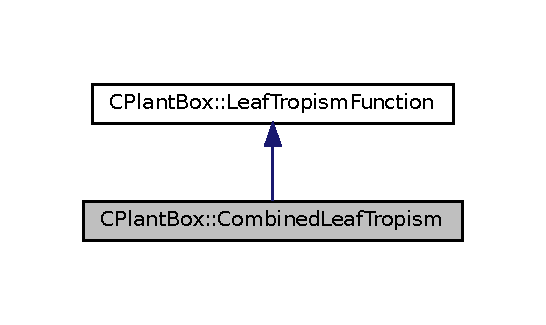
\includegraphics[width=262pt]{classCPlantBox_1_1CombinedLeafTropism__inherit__graph}
\end{center}
\end{figure}


Collaboration diagram for C\+Plant\+Box\+:\+:Combined\+Leaf\+Tropism\+:\nopagebreak
\begin{figure}[H]
\begin{center}
\leavevmode
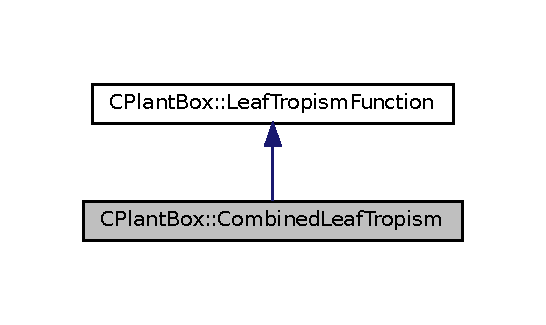
\includegraphics[width=262pt]{classCPlantBox_1_1CombinedLeafTropism__coll__graph}
\end{center}
\end{figure}
\subsection*{Public Member Functions}
\begin{DoxyCompactItemize}
\item 
\mbox{\Hypertarget{classCPlantBox_1_1CombinedLeafTropism_a864af63cb3897d5d7793f23df84f9049}\label{classCPlantBox_1_1CombinedLeafTropism_a864af63cb3897d5d7793f23df84f9049}} 
\hyperlink{classCPlantBox_1_1CombinedLeafTropism_a864af63cb3897d5d7793f23df84f9049}{Combined\+Leaf\+Tropism} (double \hyperlink{classCPlantBox_1_1LeafTropismFunction_a21d8d756f8b9f6015b546def33b01c89}{n}, double \hyperlink{classCPlantBox_1_1LeafTropismFunction_a82a3dc11056a65501bc4535749c304b6}{sigma}, std\+::vector$<$ \hyperlink{classCPlantBox_1_1LeafTropismFunction}{Leaf\+Tropism\+Function} $\ast$$>$ tropisms\+\_\+, std\+::vector$<$ double $>$ weights\+\_\+)
\begin{DoxyCompactList}\small\item\em linearly comibines the objective functions of multiple tropisms \end{DoxyCompactList}\item 
\hyperlink{classCPlantBox_1_1CombinedLeafTropism_a932f5340663a5785b31f4013fe0132aa}{Combined\+Leaf\+Tropism} (double \hyperlink{classCPlantBox_1_1LeafTropismFunction_a21d8d756f8b9f6015b546def33b01c89}{n}, double \hyperlink{classCPlantBox_1_1LeafTropismFunction_a82a3dc11056a65501bc4535749c304b6}{sigma}, \hyperlink{classCPlantBox_1_1LeafTropismFunction}{Leaf\+Tropism\+Function} $\ast$t1, double w1, \hyperlink{classCPlantBox_1_1LeafTropismFunction}{Leaf\+Tropism\+Function} $\ast$t2, double w2)
\begin{DoxyCompactList}\small\item\em linearly comibines the objective functions of two tropism funcitons \end{DoxyCompactList}\item 
virtual double \hyperlink{classCPlantBox_1_1CombinedLeafTropism_aec7a53f31265f6c10a8666d0d8647aa5}{leaftropism\+Objective} (const \hyperlink{classCPlantBox_1_1Vector3d}{Vector3d} \&pos, \hyperlink{classCPlantBox_1_1Matrix3d}{Matrix3d} old, double a, double b, double dx, const \hyperlink{classCPlantBox_1_1Organ}{Organ} $\ast$leaf) override
\begin{DoxyCompactList}\small\item\em \hyperlink{classCPlantBox_1_1LeafTropismFunction_a1440868221a834474e34e3a503a74572}{get\+Heading()} minimizes this function, \end{DoxyCompactList}\end{DoxyCompactItemize}
\subsection*{Additional Inherited Members}


\subsection{Detailed Description}
Combined tropisms, creates a linear combination of the respective objective functions 

\subsection{Constructor \& Destructor Documentation}
\mbox{\Hypertarget{classCPlantBox_1_1CombinedLeafTropism_a932f5340663a5785b31f4013fe0132aa}\label{classCPlantBox_1_1CombinedLeafTropism_a932f5340663a5785b31f4013fe0132aa}} 
\index{C\+Plant\+Box\+::\+Combined\+Leaf\+Tropism@{C\+Plant\+Box\+::\+Combined\+Leaf\+Tropism}!Combined\+Leaf\+Tropism@{Combined\+Leaf\+Tropism}}
\index{Combined\+Leaf\+Tropism@{Combined\+Leaf\+Tropism}!C\+Plant\+Box\+::\+Combined\+Leaf\+Tropism@{C\+Plant\+Box\+::\+Combined\+Leaf\+Tropism}}
\subsubsection{\texorpdfstring{Combined\+Leaf\+Tropism()}{CombinedLeafTropism()}}
{\footnotesize\ttfamily C\+Plant\+Box\+::\+Combined\+Leaf\+Tropism\+::\+Combined\+Leaf\+Tropism (\begin{DoxyParamCaption}\item[{double}]{n,  }\item[{double}]{sigma,  }\item[{\hyperlink{classCPlantBox_1_1LeafTropismFunction}{Leaf\+Tropism\+Function} $\ast$}]{t1,  }\item[{double}]{w1,  }\item[{\hyperlink{classCPlantBox_1_1LeafTropismFunction}{Leaf\+Tropism\+Function} $\ast$}]{t2,  }\item[{double}]{w2 }\end{DoxyParamCaption})}



linearly comibines the objective functions of two tropism funcitons 

Constructs a combined tropism with two tropsims, the new objective funciton is (t1-\/$>$tropism\+Objective()$\ast$w1)+(t2-\/$>$tropism\+Objective()$\ast$w2)


\begin{DoxyParams}{Parameters}
{\em n} & number of tries \\
\hline
{\em sigma} & standard deviation of angular change \mbox{[}1/cm\mbox{]} \\
\hline
{\em t1} & first tropism \\
\hline
{\em w1} & first weight \\
\hline
{\em t2} & first tropism \\
\hline
{\em w2} & first weight \\
\hline
\end{DoxyParams}


\subsection{Member Function Documentation}
\mbox{\Hypertarget{classCPlantBox_1_1CombinedLeafTropism_aec7a53f31265f6c10a8666d0d8647aa5}\label{classCPlantBox_1_1CombinedLeafTropism_aec7a53f31265f6c10a8666d0d8647aa5}} 
\index{C\+Plant\+Box\+::\+Combined\+Leaf\+Tropism@{C\+Plant\+Box\+::\+Combined\+Leaf\+Tropism}!leaftropism\+Objective@{leaftropism\+Objective}}
\index{leaftropism\+Objective@{leaftropism\+Objective}!C\+Plant\+Box\+::\+Combined\+Leaf\+Tropism@{C\+Plant\+Box\+::\+Combined\+Leaf\+Tropism}}
\subsubsection{\texorpdfstring{leaftropism\+Objective()}{leaftropismObjective()}}
{\footnotesize\ttfamily double C\+Plant\+Box\+::\+Combined\+Leaf\+Tropism\+::leaftropism\+Objective (\begin{DoxyParamCaption}\item[{const \hyperlink{classCPlantBox_1_1Vector3d}{Vector3d} \&}]{pos,  }\item[{\hyperlink{classCPlantBox_1_1Matrix3d}{Matrix3d}}]{old,  }\item[{double}]{a,  }\item[{double}]{b,  }\item[{double}]{dx,  }\item[{const \hyperlink{classCPlantBox_1_1Organ}{Organ} $\ast$}]{leaf }\end{DoxyParamCaption})\hspace{0.3cm}{\ttfamily [override]}, {\ttfamily [virtual]}}



\hyperlink{classCPlantBox_1_1LeafTropismFunction_a1440868221a834474e34e3a503a74572}{get\+Heading()} minimizes this function, 

\begin{DoxySeeAlso}{See also}
\hyperlink{classCPlantBox_1_1TropismFunction}{Tropism\+Function}
\end{DoxySeeAlso}
\hyperlink{classCPlantBox_1_1LeafTropismFunction_a1440868221a834474e34e3a503a74572}{get\+Heading()} minimizes this function, \begin{DoxySeeAlso}{See also}
\hyperlink{classCPlantBox_1_1TropismFunction_a4f2c79fff55d1398c98a070dd8ebbe08}{Tropism\+Function\+::tropism\+Objective} 
\end{DoxySeeAlso}


Reimplemented from \hyperlink{classCPlantBox_1_1LeafTropismFunction_ab89f5f7e80103d80681bc8cadc220dba}{C\+Plant\+Box\+::\+Leaf\+Tropism\+Function}.



The documentation for this class was generated from the following files\+:\begin{DoxyCompactItemize}
\item 
src/Leaf\+Tropism.\+h\item 
src/Leaf\+Tropism.\+cpp\end{DoxyCompactItemize}

\hypertarget{classCPlantBox_1_1CombinedStemTropism}{}\section{C\+Plant\+Box\+:\+:Combined\+Stem\+Tropism Class Reference}
\label{classCPlantBox_1_1CombinedStemTropism}\index{C\+Plant\+Box\+::\+Combined\+Stem\+Tropism@{C\+Plant\+Box\+::\+Combined\+Stem\+Tropism}}


{\ttfamily \#include $<$Stem\+Tropism.\+h$>$}



Inheritance diagram for C\+Plant\+Box\+:\+:Combined\+Stem\+Tropism\+:\nopagebreak
\begin{figure}[H]
\begin{center}
\leavevmode
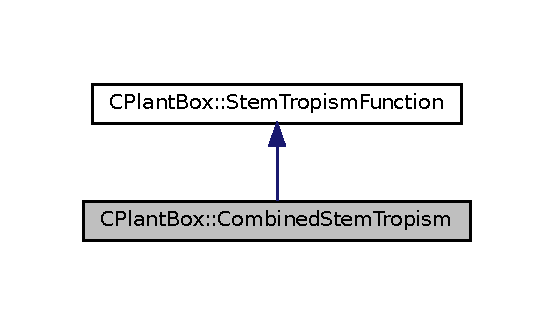
\includegraphics[width=266pt]{classCPlantBox_1_1CombinedStemTropism__inherit__graph}
\end{center}
\end{figure}


Collaboration diagram for C\+Plant\+Box\+:\+:Combined\+Stem\+Tropism\+:\nopagebreak
\begin{figure}[H]
\begin{center}
\leavevmode
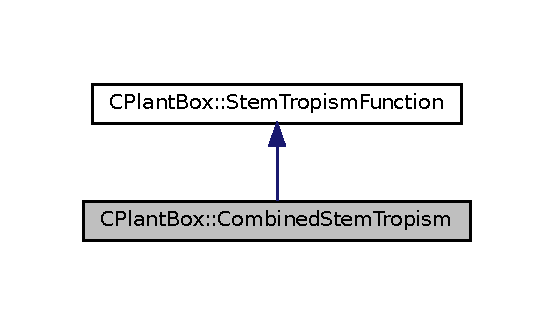
\includegraphics[width=266pt]{classCPlantBox_1_1CombinedStemTropism__coll__graph}
\end{center}
\end{figure}
\subsection*{Public Member Functions}
\begin{DoxyCompactItemize}
\item 
\mbox{\Hypertarget{classCPlantBox_1_1CombinedStemTropism_a5098b097bfa24475628bafaf7d3f2df8}\label{classCPlantBox_1_1CombinedStemTropism_a5098b097bfa24475628bafaf7d3f2df8}} 
\hyperlink{classCPlantBox_1_1CombinedStemTropism_a5098b097bfa24475628bafaf7d3f2df8}{Combined\+Stem\+Tropism} (double \hyperlink{classCPlantBox_1_1StemTropismFunction_a54ebffbb66feb026ce61d57f17d4d25a}{n}, double \hyperlink{classCPlantBox_1_1StemTropismFunction_a79ea448c44b07fb59d85e9d130190994}{sigma}, std\+::vector$<$ \hyperlink{classCPlantBox_1_1StemTropismFunction}{Stem\+Tropism\+Function} $\ast$$>$ tropisms\+\_\+, std\+::vector$<$ double $>$ weights\+\_\+)
\begin{DoxyCompactList}\small\item\em linearly comibines the objective functions of multiple tropisms \end{DoxyCompactList}\item 
\hyperlink{classCPlantBox_1_1CombinedStemTropism_ae3d20067c6cd334b68daa7c6608a6f76}{Combined\+Stem\+Tropism} (double \hyperlink{classCPlantBox_1_1StemTropismFunction_a54ebffbb66feb026ce61d57f17d4d25a}{n}, double \hyperlink{classCPlantBox_1_1StemTropismFunction_a79ea448c44b07fb59d85e9d130190994}{sigma}, \hyperlink{classCPlantBox_1_1StemTropismFunction}{Stem\+Tropism\+Function} $\ast$t1, double w1, \hyperlink{classCPlantBox_1_1StemTropismFunction}{Stem\+Tropism\+Function} $\ast$t2, double w2)
\begin{DoxyCompactList}\small\item\em linearly comibines the objective functions of two tropism funcitons \end{DoxyCompactList}\item 
virtual double \hyperlink{classCPlantBox_1_1CombinedStemTropism_abe3aa8ad9529b57d002e7c6407c575c2}{stemtropism\+Objective} (const \hyperlink{classCPlantBox_1_1Vector3d}{Vector3d} \&pos, \hyperlink{classCPlantBox_1_1Matrix3d}{Matrix3d} old, double a, double b, double dx, const \hyperlink{classCPlantBox_1_1Organ}{Organ} $\ast$stem) override
\begin{DoxyCompactList}\small\item\em \hyperlink{classCPlantBox_1_1StemTropismFunction_ac72f7ad1200d1defbb3c9b20e20d1f62}{get\+Heading()} minimizes this function, \end{DoxyCompactList}\end{DoxyCompactItemize}
\subsection*{Additional Inherited Members}


\subsection{Detailed Description}
Combined tropisms, creates a linear combination of the respective objective functions 

\subsection{Constructor \& Destructor Documentation}
\mbox{\Hypertarget{classCPlantBox_1_1CombinedStemTropism_ae3d20067c6cd334b68daa7c6608a6f76}\label{classCPlantBox_1_1CombinedStemTropism_ae3d20067c6cd334b68daa7c6608a6f76}} 
\index{C\+Plant\+Box\+::\+Combined\+Stem\+Tropism@{C\+Plant\+Box\+::\+Combined\+Stem\+Tropism}!Combined\+Stem\+Tropism@{Combined\+Stem\+Tropism}}
\index{Combined\+Stem\+Tropism@{Combined\+Stem\+Tropism}!C\+Plant\+Box\+::\+Combined\+Stem\+Tropism@{C\+Plant\+Box\+::\+Combined\+Stem\+Tropism}}
\subsubsection{\texorpdfstring{Combined\+Stem\+Tropism()}{CombinedStemTropism()}}
{\footnotesize\ttfamily C\+Plant\+Box\+::\+Combined\+Stem\+Tropism\+::\+Combined\+Stem\+Tropism (\begin{DoxyParamCaption}\item[{double}]{n,  }\item[{double}]{sigma,  }\item[{\hyperlink{classCPlantBox_1_1StemTropismFunction}{Stem\+Tropism\+Function} $\ast$}]{t1,  }\item[{double}]{w1,  }\item[{\hyperlink{classCPlantBox_1_1StemTropismFunction}{Stem\+Tropism\+Function} $\ast$}]{t2,  }\item[{double}]{w2 }\end{DoxyParamCaption})}



linearly comibines the objective functions of two tropism funcitons 

Constructs a combined tropism with two tropsims, the new objective funciton is (t1-\/$>$tropism\+Objective()$\ast$w1)+(t2-\/$>$tropism\+Objective()$\ast$w2)


\begin{DoxyParams}{Parameters}
{\em n} & number of tries \\
\hline
{\em sigma} & standard deviation of angular change \mbox{[}1/cm\mbox{]} \\
\hline
{\em t1} & first tropism \\
\hline
{\em w1} & first weight \\
\hline
{\em t2} & first tropism \\
\hline
{\em w2} & first weight \\
\hline
\end{DoxyParams}


\subsection{Member Function Documentation}
\mbox{\Hypertarget{classCPlantBox_1_1CombinedStemTropism_abe3aa8ad9529b57d002e7c6407c575c2}\label{classCPlantBox_1_1CombinedStemTropism_abe3aa8ad9529b57d002e7c6407c575c2}} 
\index{C\+Plant\+Box\+::\+Combined\+Stem\+Tropism@{C\+Plant\+Box\+::\+Combined\+Stem\+Tropism}!stemtropism\+Objective@{stemtropism\+Objective}}
\index{stemtropism\+Objective@{stemtropism\+Objective}!C\+Plant\+Box\+::\+Combined\+Stem\+Tropism@{C\+Plant\+Box\+::\+Combined\+Stem\+Tropism}}
\subsubsection{\texorpdfstring{stemtropism\+Objective()}{stemtropismObjective()}}
{\footnotesize\ttfamily double C\+Plant\+Box\+::\+Combined\+Stem\+Tropism\+::stemtropism\+Objective (\begin{DoxyParamCaption}\item[{const \hyperlink{classCPlantBox_1_1Vector3d}{Vector3d} \&}]{pos,  }\item[{\hyperlink{classCPlantBox_1_1Matrix3d}{Matrix3d}}]{old,  }\item[{double}]{a,  }\item[{double}]{b,  }\item[{double}]{dx,  }\item[{const \hyperlink{classCPlantBox_1_1Organ}{Organ} $\ast$}]{stem }\end{DoxyParamCaption})\hspace{0.3cm}{\ttfamily [override]}, {\ttfamily [virtual]}}



\hyperlink{classCPlantBox_1_1StemTropismFunction_ac72f7ad1200d1defbb3c9b20e20d1f62}{get\+Heading()} minimizes this function, 

\begin{DoxySeeAlso}{See also}
\hyperlink{classCPlantBox_1_1TropismFunction}{Tropism\+Function}
\end{DoxySeeAlso}
\hyperlink{classCPlantBox_1_1StemTropismFunction_ac72f7ad1200d1defbb3c9b20e20d1f62}{get\+Heading()} minimizes this function, \begin{DoxySeeAlso}{See also}
\hyperlink{classCPlantBox_1_1TropismFunction_a4f2c79fff55d1398c98a070dd8ebbe08}{Tropism\+Function\+::tropism\+Objective} 
\end{DoxySeeAlso}


Reimplemented from \hyperlink{classCPlantBox_1_1StemTropismFunction_a86dc37330cbec72042352dcce88756ae}{C\+Plant\+Box\+::\+Stem\+Tropism\+Function}.



The documentation for this class was generated from the following files\+:\begin{DoxyCompactItemize}
\item 
src/Stem\+Tropism.\+h\item 
src/Stem\+Tropism.\+cpp\end{DoxyCompactItemize}

\hypertarget{classCPlantBox_1_1CombinedTropism}{}\section{C\+Plant\+Box\+:\+:Combined\+Tropism Class Reference}
\label{classCPlantBox_1_1CombinedTropism}\index{C\+Plant\+Box\+::\+Combined\+Tropism@{C\+Plant\+Box\+::\+Combined\+Tropism}}


{\ttfamily \#include $<$Root\+Tropism.\+h$>$}



Inheritance diagram for C\+Plant\+Box\+:\+:Combined\+Tropism\+:\nopagebreak
\begin{figure}[H]
\begin{center}
\leavevmode
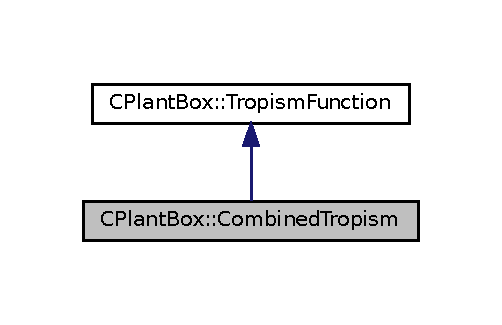
\includegraphics[width=241pt]{classCPlantBox_1_1CombinedTropism__inherit__graph}
\end{center}
\end{figure}


Collaboration diagram for C\+Plant\+Box\+:\+:Combined\+Tropism\+:\nopagebreak
\begin{figure}[H]
\begin{center}
\leavevmode
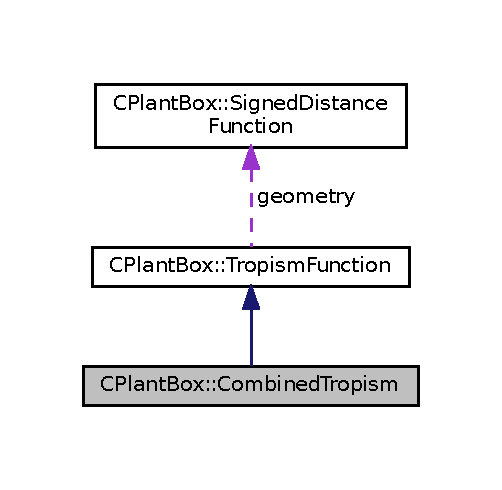
\includegraphics[width=241pt]{classCPlantBox_1_1CombinedTropism__coll__graph}
\end{center}
\end{figure}
\subsection*{Public Member Functions}
\begin{DoxyCompactItemize}
\item 
\mbox{\Hypertarget{classCPlantBox_1_1CombinedTropism_ace109481909098acc9e430706368d0c5}\label{classCPlantBox_1_1CombinedTropism_ace109481909098acc9e430706368d0c5}} 
\hyperlink{classCPlantBox_1_1CombinedTropism_ace109481909098acc9e430706368d0c5}{Combined\+Tropism} (double \hyperlink{classCPlantBox_1_1TropismFunction_a619c74d63319c406730c95679784a04a}{n}, double \hyperlink{classCPlantBox_1_1TropismFunction_acdc5f9c3beda0a74ddadd591c5d8afaf}{sigma}, std\+::vector$<$ \hyperlink{classCPlantBox_1_1TropismFunction}{Tropism\+Function} $\ast$$>$ tropisms\+\_\+, std\+::vector$<$ double $>$ weights\+\_\+)
\begin{DoxyCompactList}\small\item\em linearly comibines the objective functions of multiple tropisms \end{DoxyCompactList}\item 
\hyperlink{classCPlantBox_1_1CombinedTropism_a5c02c15e17677871efaa7b8cfbc6c9b6}{Combined\+Tropism} (double \hyperlink{classCPlantBox_1_1TropismFunction_a619c74d63319c406730c95679784a04a}{n}, double \hyperlink{classCPlantBox_1_1TropismFunction_acdc5f9c3beda0a74ddadd591c5d8afaf}{sigma}, \hyperlink{classCPlantBox_1_1TropismFunction}{Tropism\+Function} $\ast$t1, double w1, \hyperlink{classCPlantBox_1_1TropismFunction}{Tropism\+Function} $\ast$t2, double w2)
\begin{DoxyCompactList}\small\item\em linearly comibines the objective functions of two tropism funcitons \end{DoxyCompactList}\item 
\mbox{\Hypertarget{classCPlantBox_1_1CombinedTropism_a4fee2980c11652ac13d5652bdcd47d87}\label{classCPlantBox_1_1CombinedTropism_a4fee2980c11652ac13d5652bdcd47d87}} 
virtual \hyperlink{classCPlantBox_1_1TropismFunction}{Tropism\+Function} $\ast$ \hyperlink{classCPlantBox_1_1CombinedTropism_a4fee2980c11652ac13d5652bdcd47d87}{copy} () override
\begin{DoxyCompactList}\small\item\em copy constructor \end{DoxyCompactList}\item 
virtual double \hyperlink{classCPlantBox_1_1CombinedTropism_a9ed761842ac79d92c15f9a88fc2df995}{tropism\+Objective} (const \hyperlink{classCPlantBox_1_1Vector3d}{Vector3d} \&pos, \hyperlink{classCPlantBox_1_1Matrix3d}{Matrix3d} old, double a, double b, double dx, const \hyperlink{classCPlantBox_1_1Organ}{Organ} $\ast$root) override
\begin{DoxyCompactList}\small\item\em \hyperlink{classCPlantBox_1_1TropismFunction_adb52b88734a94fe1365a00e02c7e6be5}{get\+Heading()} minimizes this function, \end{DoxyCompactList}\end{DoxyCompactItemize}
\subsection*{Additional Inherited Members}


\subsection{Detailed Description}
Combined tropisms, creates a linear combination of the respective objective functions 

\subsection{Constructor \& Destructor Documentation}
\mbox{\Hypertarget{classCPlantBox_1_1CombinedTropism_a5c02c15e17677871efaa7b8cfbc6c9b6}\label{classCPlantBox_1_1CombinedTropism_a5c02c15e17677871efaa7b8cfbc6c9b6}} 
\index{C\+Plant\+Box\+::\+Combined\+Tropism@{C\+Plant\+Box\+::\+Combined\+Tropism}!Combined\+Tropism@{Combined\+Tropism}}
\index{Combined\+Tropism@{Combined\+Tropism}!C\+Plant\+Box\+::\+Combined\+Tropism@{C\+Plant\+Box\+::\+Combined\+Tropism}}
\subsubsection{\texorpdfstring{Combined\+Tropism()}{CombinedTropism()}}
{\footnotesize\ttfamily C\+Plant\+Box\+::\+Combined\+Tropism\+::\+Combined\+Tropism (\begin{DoxyParamCaption}\item[{double}]{n,  }\item[{double}]{sigma,  }\item[{\hyperlink{classCPlantBox_1_1TropismFunction}{Tropism\+Function} $\ast$}]{t1,  }\item[{double}]{w1,  }\item[{\hyperlink{classCPlantBox_1_1TropismFunction}{Tropism\+Function} $\ast$}]{t2,  }\item[{double}]{w2 }\end{DoxyParamCaption})}



linearly comibines the objective functions of two tropism funcitons 

Constructs a combined tropism with two tropsims, the new objective funciton is (t1-\/$>$\hyperlink{classCPlantBox_1_1CombinedTropism_a9ed761842ac79d92c15f9a88fc2df995}{tropism\+Objective()}$\ast$w1)+(t2-\/$>$\hyperlink{classCPlantBox_1_1CombinedTropism_a9ed761842ac79d92c15f9a88fc2df995}{tropism\+Objective()}$\ast$w2)


\begin{DoxyParams}{Parameters}
{\em n} & number of tries \\
\hline
{\em sigma} & standard deviation of angular change \mbox{[}1/cm\mbox{]} \\
\hline
{\em t1} & first tropism \\
\hline
{\em w1} & first weight \\
\hline
{\em t2} & first tropism \\
\hline
{\em w2} & first weight \\
\hline
\end{DoxyParams}


\subsection{Member Function Documentation}
\mbox{\Hypertarget{classCPlantBox_1_1CombinedTropism_a9ed761842ac79d92c15f9a88fc2df995}\label{classCPlantBox_1_1CombinedTropism_a9ed761842ac79d92c15f9a88fc2df995}} 
\index{C\+Plant\+Box\+::\+Combined\+Tropism@{C\+Plant\+Box\+::\+Combined\+Tropism}!tropism\+Objective@{tropism\+Objective}}
\index{tropism\+Objective@{tropism\+Objective}!C\+Plant\+Box\+::\+Combined\+Tropism@{C\+Plant\+Box\+::\+Combined\+Tropism}}
\subsubsection{\texorpdfstring{tropism\+Objective()}{tropismObjective()}}
{\footnotesize\ttfamily double C\+Plant\+Box\+::\+Combined\+Tropism\+::tropism\+Objective (\begin{DoxyParamCaption}\item[{const \hyperlink{classCPlantBox_1_1Vector3d}{Vector3d} \&}]{pos,  }\item[{\hyperlink{classCPlantBox_1_1Matrix3d}{Matrix3d}}]{old,  }\item[{double}]{a,  }\item[{double}]{b,  }\item[{double}]{dx,  }\item[{const \hyperlink{classCPlantBox_1_1Organ}{Organ} $\ast$}]{root }\end{DoxyParamCaption})\hspace{0.3cm}{\ttfamily [override]}, {\ttfamily [virtual]}}



\hyperlink{classCPlantBox_1_1TropismFunction_adb52b88734a94fe1365a00e02c7e6be5}{get\+Heading()} minimizes this function, 

\begin{DoxySeeAlso}{See also}
\hyperlink{classCPlantBox_1_1TropismFunction}{Tropism\+Function}
\end{DoxySeeAlso}
\hyperlink{classCPlantBox_1_1TropismFunction_adb52b88734a94fe1365a00e02c7e6be5}{get\+Heading()} minimizes this function, \begin{DoxySeeAlso}{See also}
\hyperlink{classCPlantBox_1_1TropismFunction_a4f2c79fff55d1398c98a070dd8ebbe08}{Tropism\+Function\+::tropism\+Objective} 
\end{DoxySeeAlso}


Reimplemented from \hyperlink{classCPlantBox_1_1TropismFunction_a4f2c79fff55d1398c98a070dd8ebbe08}{C\+Plant\+Box\+::\+Tropism\+Function}.



The documentation for this class was generated from the following files\+:\begin{DoxyCompactItemize}
\item 
src/Root\+Tropism.\+h\item 
src/Root\+Tropism.\+cpp\end{DoxyCompactItemize}

\hypertarget{classCPlantBox_1_1ConfinedLeafTropism}{}\section{C\+Plant\+Box\+:\+:Confined\+Leaf\+Tropism Class Reference}
\label{classCPlantBox_1_1ConfinedLeafTropism}\index{C\+Plant\+Box\+::\+Confined\+Leaf\+Tropism@{C\+Plant\+Box\+::\+Confined\+Leaf\+Tropism}}


{\ttfamily \#include $<$Leaf\+Tropism.\+h$>$}



Inheritance diagram for C\+Plant\+Box\+:\+:Confined\+Leaf\+Tropism\+:\nopagebreak
\begin{figure}[H]
\begin{center}
\leavevmode
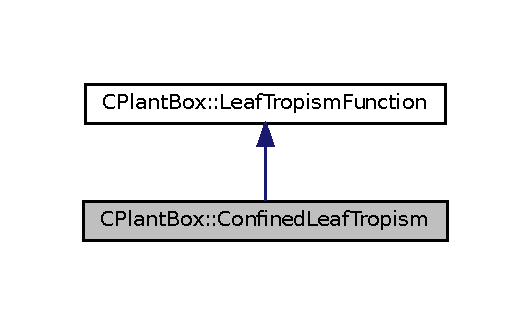
\includegraphics[width=255pt]{classCPlantBox_1_1ConfinedLeafTropism__inherit__graph}
\end{center}
\end{figure}


Collaboration diagram for C\+Plant\+Box\+:\+:Confined\+Leaf\+Tropism\+:\nopagebreak
\begin{figure}[H]
\begin{center}
\leavevmode
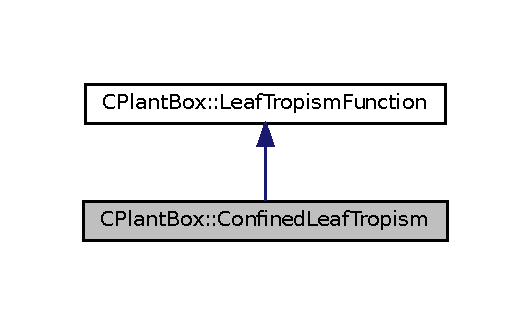
\includegraphics[width=255pt]{classCPlantBox_1_1ConfinedLeafTropism__coll__graph}
\end{center}
\end{figure}
\subsection*{Public Member Functions}
\begin{DoxyCompactItemize}
\item 
\hyperlink{classCPlantBox_1_1ConfinedLeafTropism_a4edff5fe35c9f489f4e86ac972c362d2}{Confined\+Leaf\+Tropism} (\hyperlink{classCPlantBox_1_1LeafTropismFunction}{Leaf\+Tropism\+Function} $\ast$base\+Tropism, \hyperlink{classCPlantBox_1_1SignedDistanceFunction}{Signed\+Distance\+Function} $\ast$geometry)
\item 
virtual \hyperlink{classCPlantBox_1_1Vector2d}{Vector2d} \hyperlink{classCPlantBox_1_1ConfinedLeafTropism_a0574aa544341937fc9df37a972cd0833}{get\+Heading} (const \hyperlink{classCPlantBox_1_1Vector3d}{Vector3d} \&pos, \hyperlink{classCPlantBox_1_1Matrix3d}{Matrix3d} old, double dx, const \hyperlink{classCPlantBox_1_1Organ}{Organ} $\ast$leaf) override
\begin{DoxyCompactList}\small\item\em changes base\+Tropism-\/$>$\hyperlink{classCPlantBox_1_1ConfinedLeafTropism_a0574aa544341937fc9df37a972cd0833}{get\+Heading()} in case geometric boundaries are hit \end{DoxyCompactList}\item 
\mbox{\Hypertarget{classCPlantBox_1_1ConfinedLeafTropism_afaa130b76e027bd9c21fe1938ecf9067}\label{classCPlantBox_1_1ConfinedLeafTropism_afaa130b76e027bd9c21fe1938ecf9067}} 
virtual double \hyperlink{classCPlantBox_1_1ConfinedLeafTropism_afaa130b76e027bd9c21fe1938ecf9067}{leaftropism\+Objective} (const \hyperlink{classCPlantBox_1_1Vector3d}{Vector3d} \&pos, \hyperlink{classCPlantBox_1_1Matrix3d}{Matrix3d} old, double a, double b, double dx, const \hyperlink{classCPlantBox_1_1Organ}{Organ} $\ast$leaf) override
\begin{DoxyCompactList}\small\item\em this mehtod is not called, instead base\+Tropism-\/$>$tropism\+Objective() is used by get\+Heading \end{DoxyCompactList}\end{DoxyCompactItemize}
\subsection*{Additional Inherited Members}


\subsection{Detailed Description}
Confines root growth to a geometry 

\subsection{Constructor \& Destructor Documentation}
\mbox{\Hypertarget{classCPlantBox_1_1ConfinedLeafTropism_a4edff5fe35c9f489f4e86ac972c362d2}\label{classCPlantBox_1_1ConfinedLeafTropism_a4edff5fe35c9f489f4e86ac972c362d2}} 
\index{C\+Plant\+Box\+::\+Confined\+Leaf\+Tropism@{C\+Plant\+Box\+::\+Confined\+Leaf\+Tropism}!Confined\+Leaf\+Tropism@{Confined\+Leaf\+Tropism}}
\index{Confined\+Leaf\+Tropism@{Confined\+Leaf\+Tropism}!C\+Plant\+Box\+::\+Confined\+Leaf\+Tropism@{C\+Plant\+Box\+::\+Confined\+Leaf\+Tropism}}
\subsubsection{\texorpdfstring{Confined\+Leaf\+Tropism()}{ConfinedLeafTropism()}}
{\footnotesize\ttfamily C\+Plant\+Box\+::\+Confined\+Leaf\+Tropism\+::\+Confined\+Leaf\+Tropism (\begin{DoxyParamCaption}\item[{\hyperlink{classCPlantBox_1_1LeafTropismFunction}{Leaf\+Tropism\+Function} $\ast$}]{base\+Tropism,  }\item[{\hyperlink{classCPlantBox_1_1SignedDistanceFunction}{Signed\+Distance\+Function} $\ast$}]{geometry }\end{DoxyParamCaption})\hspace{0.3cm}{\ttfamily [inline]}}

\hyperlink{classCPlantBox_1_1ConfinedTropism}{Confined\+Tropism} confines a tropism to a geometry given by a signed distance function


\begin{DoxyParams}{Parameters}
{\em base\+Tropism} & the underlying tropism \\
\hline
{\em geometry} & geometry, e.\+g. of a plant container or an obstacle \\
\hline
\end{DoxyParams}


\subsection{Member Function Documentation}
\mbox{\Hypertarget{classCPlantBox_1_1ConfinedLeafTropism_a0574aa544341937fc9df37a972cd0833}\label{classCPlantBox_1_1ConfinedLeafTropism_a0574aa544341937fc9df37a972cd0833}} 
\index{C\+Plant\+Box\+::\+Confined\+Leaf\+Tropism@{C\+Plant\+Box\+::\+Confined\+Leaf\+Tropism}!get\+Heading@{get\+Heading}}
\index{get\+Heading@{get\+Heading}!C\+Plant\+Box\+::\+Confined\+Leaf\+Tropism@{C\+Plant\+Box\+::\+Confined\+Leaf\+Tropism}}
\subsubsection{\texorpdfstring{get\+Heading()}{getHeading()}}
{\footnotesize\ttfamily \hyperlink{classCPlantBox_1_1Vector2d}{Vector2d} C\+Plant\+Box\+::\+Confined\+Leaf\+Tropism\+::get\+Heading (\begin{DoxyParamCaption}\item[{const \hyperlink{classCPlantBox_1_1Vector3d}{Vector3d} \&}]{pos,  }\item[{\hyperlink{classCPlantBox_1_1Matrix3d}{Matrix3d}}]{old,  }\item[{double}]{dx,  }\item[{const \hyperlink{classCPlantBox_1_1Organ}{Organ} $\ast$}]{leaf }\end{DoxyParamCaption})\hspace{0.3cm}{\ttfamily [override]}, {\ttfamily [virtual]}}



changes base\+Tropism-\/$>$\hyperlink{classCPlantBox_1_1ConfinedLeafTropism_a0574aa544341937fc9df37a972cd0833}{get\+Heading()} in case geometric boundaries are hit 

Inside the geometric domaint base\+Tropism\+::get\+Heading() is returned. In case geometric boundaries are hit, the rotations are modified, so that growth stays inside the domain.


\begin{DoxyParams}{Parameters}
{\em pos} & root tip postion \\
\hline
{\em old} & rotation matrix, heading is old(\+:,1) \\
\hline
{\em dx} & distance to look ahead (e.\+g in case of hydrotropism) \\
\hline
{\em root} & points to the root that called \hyperlink{classCPlantBox_1_1ConfinedLeafTropism_a0574aa544341937fc9df37a972cd0833}{get\+Heading()}, just in case something else is needed (i.\+e. iheading for exotropism)\\
\hline
\end{DoxyParams}
\begin{DoxyReturn}{Returns}
the rotations alpha and beta 
\end{DoxyReturn}


Reimplemented from \hyperlink{classCPlantBox_1_1LeafTropismFunction_a1440868221a834474e34e3a503a74572}{C\+Plant\+Box\+::\+Leaf\+Tropism\+Function}.



The documentation for this class was generated from the following files\+:\begin{DoxyCompactItemize}
\item 
src/Leaf\+Tropism.\+h\item 
src/Leaf\+Tropism.\+cpp\end{DoxyCompactItemize}

\hypertarget{classCPlantBox_1_1ConfinedStemTropism}{}\section{C\+Plant\+Box\+:\+:Confined\+Stem\+Tropism Class Reference}
\label{classCPlantBox_1_1ConfinedStemTropism}\index{C\+Plant\+Box\+::\+Confined\+Stem\+Tropism@{C\+Plant\+Box\+::\+Confined\+Stem\+Tropism}}


{\ttfamily \#include $<$Stem\+Tropism.\+h$>$}



Inheritance diagram for C\+Plant\+Box\+:\+:Confined\+Stem\+Tropism\+:\nopagebreak
\begin{figure}[H]
\begin{center}
\leavevmode
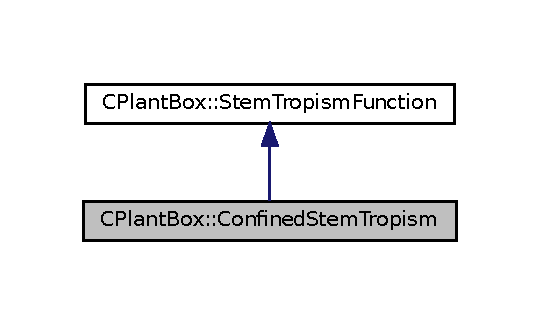
\includegraphics[width=259pt]{classCPlantBox_1_1ConfinedStemTropism__inherit__graph}
\end{center}
\end{figure}


Collaboration diagram for C\+Plant\+Box\+:\+:Confined\+Stem\+Tropism\+:\nopagebreak
\begin{figure}[H]
\begin{center}
\leavevmode
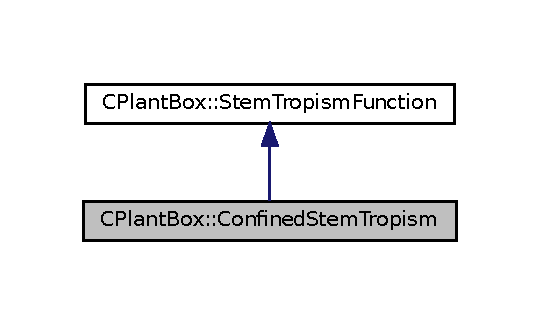
\includegraphics[width=259pt]{classCPlantBox_1_1ConfinedStemTropism__coll__graph}
\end{center}
\end{figure}
\subsection*{Public Member Functions}
\begin{DoxyCompactItemize}
\item 
\hyperlink{classCPlantBox_1_1ConfinedStemTropism_a20fe8bddeb8063c0d2649bb8ae609a25}{Confined\+Stem\+Tropism} (\hyperlink{classCPlantBox_1_1StemTropismFunction}{Stem\+Tropism\+Function} $\ast$base\+Tropism, \hyperlink{classCPlantBox_1_1SignedDistanceFunction}{Signed\+Distance\+Function} $\ast$geometry)
\item 
virtual \hyperlink{classCPlantBox_1_1Vector2d}{Vector2d} \hyperlink{classCPlantBox_1_1ConfinedStemTropism_a4c662d9319b16894fca6e5ec30461312}{get\+Heading} (const \hyperlink{classCPlantBox_1_1Vector3d}{Vector3d} \&pos, \hyperlink{classCPlantBox_1_1Matrix3d}{Matrix3d} old, double dx, const \hyperlink{classCPlantBox_1_1Organ}{Organ} $\ast$stem) override
\begin{DoxyCompactList}\small\item\em changes base\+Tropism-\/$>$\hyperlink{classCPlantBox_1_1ConfinedStemTropism_a4c662d9319b16894fca6e5ec30461312}{get\+Heading()} in case geometric boundaries are hit \end{DoxyCompactList}\item 
\mbox{\Hypertarget{classCPlantBox_1_1ConfinedStemTropism_a7adf792bf5816a82995adce13dc3b067}\label{classCPlantBox_1_1ConfinedStemTropism_a7adf792bf5816a82995adce13dc3b067}} 
virtual double \hyperlink{classCPlantBox_1_1ConfinedStemTropism_a7adf792bf5816a82995adce13dc3b067}{stemtropism\+Objective} (const \hyperlink{classCPlantBox_1_1Vector3d}{Vector3d} \&pos, \hyperlink{classCPlantBox_1_1Matrix3d}{Matrix3d} old, double a, double b, double dx, const \hyperlink{classCPlantBox_1_1Organ}{Organ} $\ast$stem) override
\begin{DoxyCompactList}\small\item\em this mehtod is not called, instead base\+Tropism-\/$>$tropism\+Objective() is used by get\+Heading \end{DoxyCompactList}\end{DoxyCompactItemize}
\subsection*{Additional Inherited Members}


\subsection{Detailed Description}
Confines root growth to a geometry 

\subsection{Constructor \& Destructor Documentation}
\mbox{\Hypertarget{classCPlantBox_1_1ConfinedStemTropism_a20fe8bddeb8063c0d2649bb8ae609a25}\label{classCPlantBox_1_1ConfinedStemTropism_a20fe8bddeb8063c0d2649bb8ae609a25}} 
\index{C\+Plant\+Box\+::\+Confined\+Stem\+Tropism@{C\+Plant\+Box\+::\+Confined\+Stem\+Tropism}!Confined\+Stem\+Tropism@{Confined\+Stem\+Tropism}}
\index{Confined\+Stem\+Tropism@{Confined\+Stem\+Tropism}!C\+Plant\+Box\+::\+Confined\+Stem\+Tropism@{C\+Plant\+Box\+::\+Confined\+Stem\+Tropism}}
\subsubsection{\texorpdfstring{Confined\+Stem\+Tropism()}{ConfinedStemTropism()}}
{\footnotesize\ttfamily C\+Plant\+Box\+::\+Confined\+Stem\+Tropism\+::\+Confined\+Stem\+Tropism (\begin{DoxyParamCaption}\item[{\hyperlink{classCPlantBox_1_1StemTropismFunction}{Stem\+Tropism\+Function} $\ast$}]{base\+Tropism,  }\item[{\hyperlink{classCPlantBox_1_1SignedDistanceFunction}{Signed\+Distance\+Function} $\ast$}]{geometry }\end{DoxyParamCaption})\hspace{0.3cm}{\ttfamily [inline]}}

\hyperlink{classCPlantBox_1_1ConfinedTropism}{Confined\+Tropism} confines a tropism to a geometry given by a signed distance function


\begin{DoxyParams}{Parameters}
{\em base\+Tropism} & the underlying tropism \\
\hline
{\em geometry} & geometry, e.\+g. of a plant container or an obstacle \\
\hline
\end{DoxyParams}


\subsection{Member Function Documentation}
\mbox{\Hypertarget{classCPlantBox_1_1ConfinedStemTropism_a4c662d9319b16894fca6e5ec30461312}\label{classCPlantBox_1_1ConfinedStemTropism_a4c662d9319b16894fca6e5ec30461312}} 
\index{C\+Plant\+Box\+::\+Confined\+Stem\+Tropism@{C\+Plant\+Box\+::\+Confined\+Stem\+Tropism}!get\+Heading@{get\+Heading}}
\index{get\+Heading@{get\+Heading}!C\+Plant\+Box\+::\+Confined\+Stem\+Tropism@{C\+Plant\+Box\+::\+Confined\+Stem\+Tropism}}
\subsubsection{\texorpdfstring{get\+Heading()}{getHeading()}}
{\footnotesize\ttfamily \hyperlink{classCPlantBox_1_1Vector2d}{Vector2d} C\+Plant\+Box\+::\+Confined\+Stem\+Tropism\+::get\+Heading (\begin{DoxyParamCaption}\item[{const \hyperlink{classCPlantBox_1_1Vector3d}{Vector3d} \&}]{pos,  }\item[{\hyperlink{classCPlantBox_1_1Matrix3d}{Matrix3d}}]{old,  }\item[{double}]{dx,  }\item[{const \hyperlink{classCPlantBox_1_1Organ}{Organ} $\ast$}]{stem }\end{DoxyParamCaption})\hspace{0.3cm}{\ttfamily [override]}, {\ttfamily [virtual]}}



changes base\+Tropism-\/$>$\hyperlink{classCPlantBox_1_1ConfinedStemTropism_a4c662d9319b16894fca6e5ec30461312}{get\+Heading()} in case geometric boundaries are hit 

Inside the geometric domaint base\+Tropism\+::get\+Heading() is returned. In case geometric boundaries are hit, the rotations are modified, so that growth stays inside the domain.


\begin{DoxyParams}{Parameters}
{\em pos} & root tip postion \\
\hline
{\em old} & rotation matrix, heading is old(\+:,1) \\
\hline
{\em dx} & distance to look ahead (e.\+g in case of hydrotropism) \\
\hline
{\em root} & points to the root that called \hyperlink{classCPlantBox_1_1ConfinedStemTropism_a4c662d9319b16894fca6e5ec30461312}{get\+Heading()}, just in case something else is needed (i.\+e. iheading for exotropism)\\
\hline
\end{DoxyParams}
\begin{DoxyReturn}{Returns}
the rotations alpha and beta 
\end{DoxyReturn}


Reimplemented from \hyperlink{classCPlantBox_1_1StemTropismFunction_ac72f7ad1200d1defbb3c9b20e20d1f62}{C\+Plant\+Box\+::\+Stem\+Tropism\+Function}.



The documentation for this class was generated from the following files\+:\begin{DoxyCompactItemize}
\item 
src/Stem\+Tropism.\+h\item 
src/Stem\+Tropism.\+cpp\end{DoxyCompactItemize}

\hypertarget{classCPlantBox_1_1ConfinedTropism}{}\section{C\+Plant\+Box\+:\+:Confined\+Tropism Class Reference}
\label{classCPlantBox_1_1ConfinedTropism}\index{C\+Plant\+Box\+::\+Confined\+Tropism@{C\+Plant\+Box\+::\+Confined\+Tropism}}


{\ttfamily \#include $<$Root\+Tropism.\+h$>$}



Inheritance diagram for C\+Plant\+Box\+:\+:Confined\+Tropism\+:\nopagebreak
\begin{figure}[H]
\begin{center}
\leavevmode
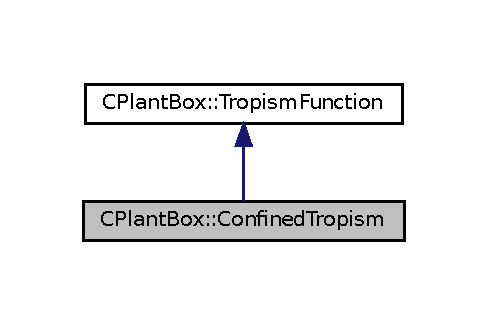
\includegraphics[width=234pt]{classCPlantBox_1_1ConfinedTropism__inherit__graph}
\end{center}
\end{figure}


Collaboration diagram for C\+Plant\+Box\+:\+:Confined\+Tropism\+:\nopagebreak
\begin{figure}[H]
\begin{center}
\leavevmode
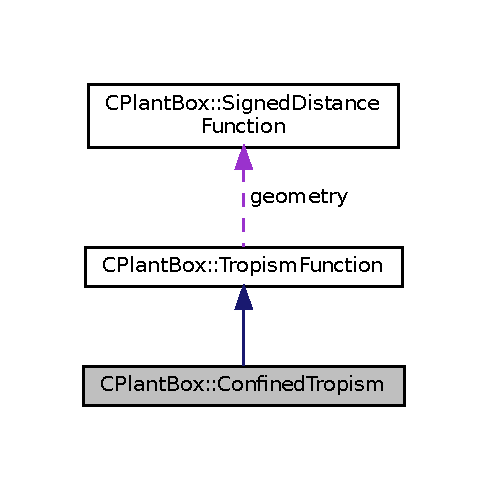
\includegraphics[width=234pt]{classCPlantBox_1_1ConfinedTropism__coll__graph}
\end{center}
\end{figure}
\subsection*{Public Member Functions}
\begin{DoxyCompactItemize}
\item 
\hyperlink{classCPlantBox_1_1ConfinedTropism_a7d90df6c52e1efe154e8e1d9f34a44fb}{Confined\+Tropism} (\hyperlink{classCPlantBox_1_1TropismFunction}{Tropism\+Function} $\ast$base\+Tropism, \hyperlink{classCPlantBox_1_1SignedDistanceFunction}{Signed\+Distance\+Function} $\ast$geometry)
\item 
virtual \hyperlink{classCPlantBox_1_1Vector2d}{Vector2d} \hyperlink{classCPlantBox_1_1ConfinedTropism_abc56888ea510bc66369c36df3d43ce42}{get\+Heading} (const \hyperlink{classCPlantBox_1_1Vector3d}{Vector3d} \&pos, \hyperlink{classCPlantBox_1_1Matrix3d}{Matrix3d} old, double dx, const \hyperlink{classCPlantBox_1_1Organ}{Organ} $\ast$root) override
\begin{DoxyCompactList}\small\item\em changes base\+Tropism-\/$>$\hyperlink{classCPlantBox_1_1ConfinedTropism_abc56888ea510bc66369c36df3d43ce42}{get\+Heading()} in case geometric boundaries are hit \end{DoxyCompactList}\item 
\mbox{\Hypertarget{classCPlantBox_1_1ConfinedTropism_ad0687d23227c9e52af8873a6d8ab8065}\label{classCPlantBox_1_1ConfinedTropism_ad0687d23227c9e52af8873a6d8ab8065}} 
virtual \hyperlink{classCPlantBox_1_1TropismFunction}{Tropism\+Function} $\ast$ \hyperlink{classCPlantBox_1_1ConfinedTropism_ad0687d23227c9e52af8873a6d8ab8065}{copy} () override
\begin{DoxyCompactList}\small\item\em copy constructor \end{DoxyCompactList}\item 
\mbox{\Hypertarget{classCPlantBox_1_1ConfinedTropism_aaa264e2b61755ecaf9baf5f6c43487e0}\label{classCPlantBox_1_1ConfinedTropism_aaa264e2b61755ecaf9baf5f6c43487e0}} 
virtual double \hyperlink{classCPlantBox_1_1ConfinedTropism_aaa264e2b61755ecaf9baf5f6c43487e0}{tropism\+Objective} (const \hyperlink{classCPlantBox_1_1Vector3d}{Vector3d} \&pos, \hyperlink{classCPlantBox_1_1Matrix3d}{Matrix3d} old, double a, double b, double dx, const \hyperlink{classCPlantBox_1_1Organ}{Organ} $\ast$root) override
\begin{DoxyCompactList}\small\item\em this mehtod is not called, instead base\+Tropism-\/$>$\hyperlink{classCPlantBox_1_1ConfinedTropism_aaa264e2b61755ecaf9baf5f6c43487e0}{tropism\+Objective()} is used by get\+Heading \end{DoxyCompactList}\end{DoxyCompactItemize}
\subsection*{Additional Inherited Members}


\subsection{Detailed Description}
Confines root growth to a geometry 

\subsection{Constructor \& Destructor Documentation}
\mbox{\Hypertarget{classCPlantBox_1_1ConfinedTropism_a7d90df6c52e1efe154e8e1d9f34a44fb}\label{classCPlantBox_1_1ConfinedTropism_a7d90df6c52e1efe154e8e1d9f34a44fb}} 
\index{C\+Plant\+Box\+::\+Confined\+Tropism@{C\+Plant\+Box\+::\+Confined\+Tropism}!Confined\+Tropism@{Confined\+Tropism}}
\index{Confined\+Tropism@{Confined\+Tropism}!C\+Plant\+Box\+::\+Confined\+Tropism@{C\+Plant\+Box\+::\+Confined\+Tropism}}
\subsubsection{\texorpdfstring{Confined\+Tropism()}{ConfinedTropism()}}
{\footnotesize\ttfamily C\+Plant\+Box\+::\+Confined\+Tropism\+::\+Confined\+Tropism (\begin{DoxyParamCaption}\item[{\hyperlink{classCPlantBox_1_1TropismFunction}{Tropism\+Function} $\ast$}]{base\+Tropism,  }\item[{\hyperlink{classCPlantBox_1_1SignedDistanceFunction}{Signed\+Distance\+Function} $\ast$}]{geometry }\end{DoxyParamCaption})\hspace{0.3cm}{\ttfamily [inline]}}

\hyperlink{classCPlantBox_1_1ConfinedTropism}{Confined\+Tropism} confines a tropism to a geometry given by a signed distance function


\begin{DoxyParams}{Parameters}
{\em base\+Tropism} & the underlying tropism \\
\hline
{\em geometry} & geometry, e.\+g. of a plant container or an obstacle \\
\hline
\end{DoxyParams}


\subsection{Member Function Documentation}
\mbox{\Hypertarget{classCPlantBox_1_1ConfinedTropism_abc56888ea510bc66369c36df3d43ce42}\label{classCPlantBox_1_1ConfinedTropism_abc56888ea510bc66369c36df3d43ce42}} 
\index{C\+Plant\+Box\+::\+Confined\+Tropism@{C\+Plant\+Box\+::\+Confined\+Tropism}!get\+Heading@{get\+Heading}}
\index{get\+Heading@{get\+Heading}!C\+Plant\+Box\+::\+Confined\+Tropism@{C\+Plant\+Box\+::\+Confined\+Tropism}}
\subsubsection{\texorpdfstring{get\+Heading()}{getHeading()}}
{\footnotesize\ttfamily \hyperlink{classCPlantBox_1_1Vector2d}{Vector2d} C\+Plant\+Box\+::\+Confined\+Tropism\+::get\+Heading (\begin{DoxyParamCaption}\item[{const \hyperlink{classCPlantBox_1_1Vector3d}{Vector3d} \&}]{pos,  }\item[{\hyperlink{classCPlantBox_1_1Matrix3d}{Matrix3d}}]{old,  }\item[{double}]{dx,  }\item[{const \hyperlink{classCPlantBox_1_1Organ}{Organ} $\ast$}]{root }\end{DoxyParamCaption})\hspace{0.3cm}{\ttfamily [override]}, {\ttfamily [virtual]}}



changes base\+Tropism-\/$>$\hyperlink{classCPlantBox_1_1ConfinedTropism_abc56888ea510bc66369c36df3d43ce42}{get\+Heading()} in case geometric boundaries are hit 

Inside the geometric domaint base\+Tropism\+::get\+Heading() is returned. In case geometric boundaries are hit, the rotations are modified, so that growth stays inside the domain.


\begin{DoxyParams}{Parameters}
{\em pos} & root tip postion \\
\hline
{\em old} & rotation matrix, heading is old(\+:,1) \\
\hline
{\em dx} & distance to look ahead (e.\+g in case of hydrotropism) \\
\hline
{\em root} & points to the root that called \hyperlink{classCPlantBox_1_1ConfinedTropism_abc56888ea510bc66369c36df3d43ce42}{get\+Heading()}, just in case something else is needed (i.\+e. iheading for exotropism)\\
\hline
\end{DoxyParams}
\begin{DoxyReturn}{Returns}
the rotations alpha and beta 
\end{DoxyReturn}


Reimplemented from \hyperlink{classCPlantBox_1_1TropismFunction_adb52b88734a94fe1365a00e02c7e6be5}{C\+Plant\+Box\+::\+Tropism\+Function}.



The documentation for this class was generated from the following files\+:\begin{DoxyCompactItemize}
\item 
src/Root\+Tropism.\+h\item 
src/Root\+Tropism.\+cpp\end{DoxyCompactItemize}

\hypertarget{classCPlantBox_1_1tinyxml2_1_1DynArray}{}\section{C\+Plant\+Box\+:\+:tinyxml2\+:\+:Dyn\+Array$<$ T, I\+N\+I\+T\+I\+A\+L\+\_\+\+S\+I\+ZE $>$ Class Template Reference}
\label{classCPlantBox_1_1tinyxml2_1_1DynArray}\index{C\+Plant\+Box\+::tinyxml2\+::\+Dyn\+Array$<$ T, I\+N\+I\+T\+I\+A\+L\+\_\+\+S\+I\+Z\+E $>$@{C\+Plant\+Box\+::tinyxml2\+::\+Dyn\+Array$<$ T, I\+N\+I\+T\+I\+A\+L\+\_\+\+S\+I\+Z\+E $>$}}
\subsection*{Public Member Functions}
\begin{DoxyCompactItemize}
\item 
\mbox{\Hypertarget{classCPlantBox_1_1tinyxml2_1_1DynArray_a4e888a7930175dad2cffb7f77aadfe29}\label{classCPlantBox_1_1tinyxml2_1_1DynArray_a4e888a7930175dad2cffb7f77aadfe29}} 
void {\bfseries Clear} ()
\item 
\mbox{\Hypertarget{classCPlantBox_1_1tinyxml2_1_1DynArray_ad6c1c643f3812bfe189839f81809e22b}\label{classCPlantBox_1_1tinyxml2_1_1DynArray_ad6c1c643f3812bfe189839f81809e22b}} 
void {\bfseries Push} (T t)
\item 
\mbox{\Hypertarget{classCPlantBox_1_1tinyxml2_1_1DynArray_a77b468fe73f5b1dfa1eb4e5a12eed6b2}\label{classCPlantBox_1_1tinyxml2_1_1DynArray_a77b468fe73f5b1dfa1eb4e5a12eed6b2}} 
T $\ast$ {\bfseries Push\+Arr} (int count)
\item 
\mbox{\Hypertarget{classCPlantBox_1_1tinyxml2_1_1DynArray_a9f08a0eb0585cacd9058799b7255e0a1}\label{classCPlantBox_1_1tinyxml2_1_1DynArray_a9f08a0eb0585cacd9058799b7255e0a1}} 
T {\bfseries Pop} ()
\item 
\mbox{\Hypertarget{classCPlantBox_1_1tinyxml2_1_1DynArray_ae29b9bbe919b4e96684460e1410c2104}\label{classCPlantBox_1_1tinyxml2_1_1DynArray_ae29b9bbe919b4e96684460e1410c2104}} 
void {\bfseries Pop\+Arr} (int count)
\item 
\mbox{\Hypertarget{classCPlantBox_1_1tinyxml2_1_1DynArray_ad6fb59524f576dd34719c1f4b38d201e}\label{classCPlantBox_1_1tinyxml2_1_1DynArray_ad6fb59524f576dd34719c1f4b38d201e}} 
bool {\bfseries Empty} () const
\item 
\mbox{\Hypertarget{classCPlantBox_1_1tinyxml2_1_1DynArray_a09c53f3c31b720c609da5a582048c3bb}\label{classCPlantBox_1_1tinyxml2_1_1DynArray_a09c53f3c31b720c609da5a582048c3bb}} 
T \& {\bfseries operator\mbox{[}$\,$\mbox{]}} (int i)
\item 
\mbox{\Hypertarget{classCPlantBox_1_1tinyxml2_1_1DynArray_a2a0a7dd9b213a53d0345562c85c0b579}\label{classCPlantBox_1_1tinyxml2_1_1DynArray_a2a0a7dd9b213a53d0345562c85c0b579}} 
const T \& {\bfseries operator\mbox{[}$\,$\mbox{]}} (int i) const
\item 
\mbox{\Hypertarget{classCPlantBox_1_1tinyxml2_1_1DynArray_ad1fcf896ba95a8bc55a3feb09b07a19e}\label{classCPlantBox_1_1tinyxml2_1_1DynArray_ad1fcf896ba95a8bc55a3feb09b07a19e}} 
const T \& {\bfseries Peek\+Top} () const
\item 
\mbox{\Hypertarget{classCPlantBox_1_1tinyxml2_1_1DynArray_a43d33d2a83488a6ba624c40189dc8e7b}\label{classCPlantBox_1_1tinyxml2_1_1DynArray_a43d33d2a83488a6ba624c40189dc8e7b}} 
int {\bfseries Size} () const
\item 
\mbox{\Hypertarget{classCPlantBox_1_1tinyxml2_1_1DynArray_a172544ae6866fd3b7759c0b354afcb6a}\label{classCPlantBox_1_1tinyxml2_1_1DynArray_a172544ae6866fd3b7759c0b354afcb6a}} 
int {\bfseries Capacity} () const
\item 
\mbox{\Hypertarget{classCPlantBox_1_1tinyxml2_1_1DynArray_a35f904d96268c97ecc6d7879221ad827}\label{classCPlantBox_1_1tinyxml2_1_1DynArray_a35f904d96268c97ecc6d7879221ad827}} 
void {\bfseries Swap\+Remove} (int i)
\item 
\mbox{\Hypertarget{classCPlantBox_1_1tinyxml2_1_1DynArray_a33a3dfed2b9d5630179bc26f49121723}\label{classCPlantBox_1_1tinyxml2_1_1DynArray_a33a3dfed2b9d5630179bc26f49121723}} 
const T $\ast$ {\bfseries Mem} () const
\item 
\mbox{\Hypertarget{classCPlantBox_1_1tinyxml2_1_1DynArray_ad281b5d8a871034edf1279daa333f540}\label{classCPlantBox_1_1tinyxml2_1_1DynArray_ad281b5d8a871034edf1279daa333f540}} 
T $\ast$ {\bfseries Mem} ()
\end{DoxyCompactItemize}


The documentation for this class was generated from the following file\+:\begin{DoxyCompactItemize}
\item 
src/tinyxml2.\+h\end{DoxyCompactItemize}

\hypertarget{structCPlantBox_1_1tinyxml2_1_1Entity}{}\section{C\+Plant\+Box\+:\+:tinyxml2\+:\+:Entity Struct Reference}
\label{structCPlantBox_1_1tinyxml2_1_1Entity}\index{C\+Plant\+Box\+::tinyxml2\+::\+Entity@{C\+Plant\+Box\+::tinyxml2\+::\+Entity}}
\subsection*{Public Attributes}
\begin{DoxyCompactItemize}
\item 
\mbox{\Hypertarget{structCPlantBox_1_1tinyxml2_1_1Entity_a5c27c4610df979ddd9f4a3a1474a43a8}\label{structCPlantBox_1_1tinyxml2_1_1Entity_a5c27c4610df979ddd9f4a3a1474a43a8}} 
const char $\ast$ {\bfseries pattern}
\item 
\mbox{\Hypertarget{structCPlantBox_1_1tinyxml2_1_1Entity_a8ddf4afe02fa979373722af63497b1cd}\label{structCPlantBox_1_1tinyxml2_1_1Entity_a8ddf4afe02fa979373722af63497b1cd}} 
int {\bfseries length}
\item 
\mbox{\Hypertarget{structCPlantBox_1_1tinyxml2_1_1Entity_a721e95d54659aa54191ba3df0d42e6a7}\label{structCPlantBox_1_1tinyxml2_1_1Entity_a721e95d54659aa54191ba3df0d42e6a7}} 
char {\bfseries value}
\end{DoxyCompactItemize}


The documentation for this struct was generated from the following file\+:\begin{DoxyCompactItemize}
\item 
src/tinyxml2.\+cpp\end{DoxyCompactItemize}

\hypertarget{classCPlantBox_1_1Exotropism}{}\section{C\+Plant\+Box\+:\+:Exotropism Class Reference}
\label{classCPlantBox_1_1Exotropism}\index{C\+Plant\+Box\+::\+Exotropism@{C\+Plant\+Box\+::\+Exotropism}}


{\ttfamily \#include $<$Root\+Tropism.\+h$>$}



Inheritance diagram for C\+Plant\+Box\+:\+:Exotropism\+:\nopagebreak
\begin{figure}[H]
\begin{center}
\leavevmode
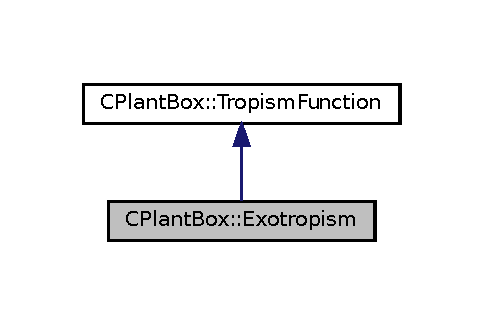
\includegraphics[width=232pt]{classCPlantBox_1_1Exotropism__inherit__graph}
\end{center}
\end{figure}


Collaboration diagram for C\+Plant\+Box\+:\+:Exotropism\+:\nopagebreak
\begin{figure}[H]
\begin{center}
\leavevmode
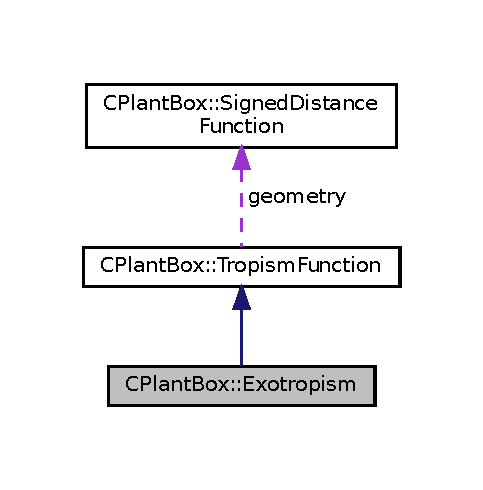
\includegraphics[width=232pt]{classCPlantBox_1_1Exotropism__coll__graph}
\end{center}
\end{figure}
\subsection*{Public Member Functions}
\begin{DoxyCompactItemize}
\item 
\hyperlink{classCPlantBox_1_1Exotropism_af2dd84113a9f66b735f5df62e658f01b}{Exotropism} (double \hyperlink{classCPlantBox_1_1TropismFunction_a619c74d63319c406730c95679784a04a}{n}, double \hyperlink{classCPlantBox_1_1TropismFunction_acdc5f9c3beda0a74ddadd591c5d8afaf}{sigma})
\item 
\mbox{\Hypertarget{classCPlantBox_1_1Exotropism_a69d3e10cbbb4eb1bd4f31f734a030950}\label{classCPlantBox_1_1Exotropism_a69d3e10cbbb4eb1bd4f31f734a030950}} 
virtual \hyperlink{classCPlantBox_1_1TropismFunction}{Tropism\+Function} $\ast$ \hyperlink{classCPlantBox_1_1Exotropism_a69d3e10cbbb4eb1bd4f31f734a030950}{copy} () override
\begin{DoxyCompactList}\small\item\em copy constructor \end{DoxyCompactList}\item 
virtual double \hyperlink{classCPlantBox_1_1Exotropism_a2049c4f5a375d90c05e9995df2e01542}{tropism\+Objective} (const \hyperlink{classCPlantBox_1_1Vector3d}{Vector3d} \&pos, \hyperlink{classCPlantBox_1_1Matrix3d}{Matrix3d} old, double a, double b, double dx, const \hyperlink{classCPlantBox_1_1Organ}{Organ} $\ast$root) override
\begin{DoxyCompactList}\small\item\em \hyperlink{classCPlantBox_1_1TropismFunction_adb52b88734a94fe1365a00e02c7e6be5}{get\+Heading()} minimizes this function, \end{DoxyCompactList}\end{DoxyCompactItemize}
\subsection*{Additional Inherited Members}


\subsection{Detailed Description}
\hyperlink{classCPlantBox_1_1Exotropism}{Exotropism}\+: the tendency to keep the initial heading 

\subsection{Constructor \& Destructor Documentation}
\mbox{\Hypertarget{classCPlantBox_1_1Exotropism_af2dd84113a9f66b735f5df62e658f01b}\label{classCPlantBox_1_1Exotropism_af2dd84113a9f66b735f5df62e658f01b}} 
\index{C\+Plant\+Box\+::\+Exotropism@{C\+Plant\+Box\+::\+Exotropism}!Exotropism@{Exotropism}}
\index{Exotropism@{Exotropism}!C\+Plant\+Box\+::\+Exotropism@{C\+Plant\+Box\+::\+Exotropism}}
\subsubsection{\texorpdfstring{Exotropism()}{Exotropism()}}
{\footnotesize\ttfamily C\+Plant\+Box\+::\+Exotropism\+::\+Exotropism (\begin{DoxyParamCaption}\item[{double}]{n,  }\item[{double}]{sigma }\end{DoxyParamCaption})\hspace{0.3cm}{\ttfamily [inline]}}

\begin{DoxySeeAlso}{See also}
\hyperlink{classCPlantBox_1_1TropismFunction}{Tropism\+Function} 
\end{DoxySeeAlso}


\subsection{Member Function Documentation}
\mbox{\Hypertarget{classCPlantBox_1_1Exotropism_a2049c4f5a375d90c05e9995df2e01542}\label{classCPlantBox_1_1Exotropism_a2049c4f5a375d90c05e9995df2e01542}} 
\index{C\+Plant\+Box\+::\+Exotropism@{C\+Plant\+Box\+::\+Exotropism}!tropism\+Objective@{tropism\+Objective}}
\index{tropism\+Objective@{tropism\+Objective}!C\+Plant\+Box\+::\+Exotropism@{C\+Plant\+Box\+::\+Exotropism}}
\subsubsection{\texorpdfstring{tropism\+Objective()}{tropismObjective()}}
{\footnotesize\ttfamily double C\+Plant\+Box\+::\+Exotropism\+::tropism\+Objective (\begin{DoxyParamCaption}\item[{const \hyperlink{classCPlantBox_1_1Vector3d}{Vector3d} \&}]{pos,  }\item[{\hyperlink{classCPlantBox_1_1Matrix3d}{Matrix3d}}]{old,  }\item[{double}]{a,  }\item[{double}]{b,  }\item[{double}]{dx,  }\item[{const \hyperlink{classCPlantBox_1_1Organ}{Organ} $\ast$}]{root }\end{DoxyParamCaption})\hspace{0.3cm}{\ttfamily [override]}, {\ttfamily [virtual]}}



\hyperlink{classCPlantBox_1_1TropismFunction_adb52b88734a94fe1365a00e02c7e6be5}{get\+Heading()} minimizes this function, 

\begin{DoxySeeAlso}{See also}
\hyperlink{classCPlantBox_1_1TropismFunction}{Tropism\+Function}
\end{DoxySeeAlso}
\hyperlink{classCPlantBox_1_1TropismFunction_adb52b88734a94fe1365a00e02c7e6be5}{get\+Heading()} minimizes this function, \begin{DoxySeeAlso}{See also}
\hyperlink{classCPlantBox_1_1TropismFunction_a4f2c79fff55d1398c98a070dd8ebbe08}{Tropism\+Function\+::tropism\+Objective} 
\end{DoxySeeAlso}


Reimplemented from \hyperlink{classCPlantBox_1_1TropismFunction_a4f2c79fff55d1398c98a070dd8ebbe08}{C\+Plant\+Box\+::\+Tropism\+Function}.



The documentation for this class was generated from the following files\+:\begin{DoxyCompactItemize}
\item 
src/Root\+Tropism.\+h\item 
src/Root\+Tropism.\+cpp\end{DoxyCompactItemize}

\hypertarget{classCPlantBox_1_1ExponentialGrowth}{}\section{C\+Plant\+Box\+:\+:Exponential\+Growth Class Reference}
\label{classCPlantBox_1_1ExponentialGrowth}\index{C\+Plant\+Box\+::\+Exponential\+Growth@{C\+Plant\+Box\+::\+Exponential\+Growth}}


{\ttfamily \#include $<$Root\+Growth.\+h$>$}



Inheritance diagram for C\+Plant\+Box\+:\+:Exponential\+Growth\+:\nopagebreak
\begin{figure}[H]
\begin{center}
\leavevmode
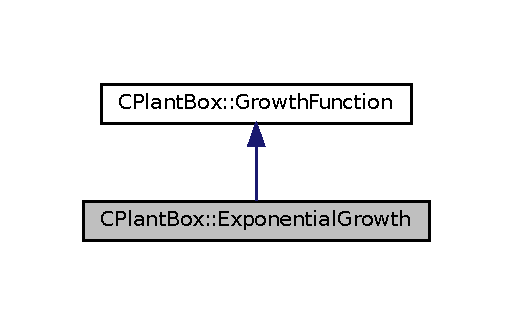
\includegraphics[width=246pt]{classCPlantBox_1_1ExponentialGrowth__inherit__graph}
\end{center}
\end{figure}


Collaboration diagram for C\+Plant\+Box\+:\+:Exponential\+Growth\+:\nopagebreak
\begin{figure}[H]
\begin{center}
\leavevmode
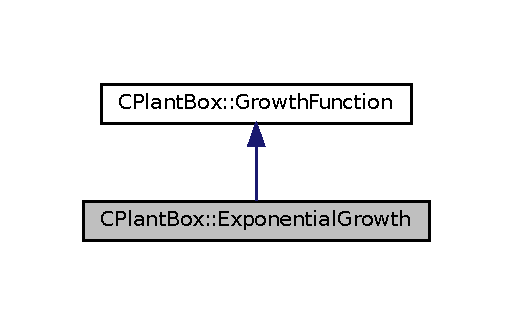
\includegraphics[width=246pt]{classCPlantBox_1_1ExponentialGrowth__coll__graph}
\end{center}
\end{figure}
\subsection*{Public Member Functions}
\begin{DoxyCompactItemize}
\item 
virtual double \hyperlink{classCPlantBox_1_1ExponentialGrowth_ae5b0f12177b71c66d199fa515698aefa}{get\+Length} (double t, double r, double k, \hyperlink{classCPlantBox_1_1Organ}{Organ} $\ast$root) const
\item 
virtual double \hyperlink{classCPlantBox_1_1ExponentialGrowth_af3fd28ae8c778bc823fc0e51756e8b63}{get\+Age} (double l, double r, double k, \hyperlink{classCPlantBox_1_1Organ}{Organ} $\ast$root) const
\end{DoxyCompactItemize}


\subsection{Detailed Description}
\hyperlink{classCPlantBox_1_1ExponentialGrowth}{Exponential\+Growth} elongates initially at constant rate r and slows down negative exponentially towards the maximum length k is reached 

\subsection{Member Function Documentation}
\mbox{\Hypertarget{classCPlantBox_1_1ExponentialGrowth_af3fd28ae8c778bc823fc0e51756e8b63}\label{classCPlantBox_1_1ExponentialGrowth_af3fd28ae8c778bc823fc0e51756e8b63}} 
\index{C\+Plant\+Box\+::\+Exponential\+Growth@{C\+Plant\+Box\+::\+Exponential\+Growth}!get\+Age@{get\+Age}}
\index{get\+Age@{get\+Age}!C\+Plant\+Box\+::\+Exponential\+Growth@{C\+Plant\+Box\+::\+Exponential\+Growth}}
\subsubsection{\texorpdfstring{get\+Age()}{getAge()}}
{\footnotesize\ttfamily virtual double C\+Plant\+Box\+::\+Exponential\+Growth\+::get\+Age (\begin{DoxyParamCaption}\item[{double}]{l,  }\item[{double}]{r,  }\item[{double}]{k,  }\item[{\hyperlink{classCPlantBox_1_1Organ}{Organ} $\ast$}]{root }\end{DoxyParamCaption}) const\hspace{0.3cm}{\ttfamily [inline]}, {\ttfamily [virtual]}}

\begin{DoxySeeAlso}{See also}
\hyperlink{classCPlantBox_1_1GrowthFunction}{Growth\+Function} 
\end{DoxySeeAlso}


Reimplemented from \hyperlink{classCPlantBox_1_1GrowthFunction_a006b428760c410389afa54853fe7cc1f}{C\+Plant\+Box\+::\+Growth\+Function}.

\mbox{\Hypertarget{classCPlantBox_1_1ExponentialGrowth_ae5b0f12177b71c66d199fa515698aefa}\label{classCPlantBox_1_1ExponentialGrowth_ae5b0f12177b71c66d199fa515698aefa}} 
\index{C\+Plant\+Box\+::\+Exponential\+Growth@{C\+Plant\+Box\+::\+Exponential\+Growth}!get\+Length@{get\+Length}}
\index{get\+Length@{get\+Length}!C\+Plant\+Box\+::\+Exponential\+Growth@{C\+Plant\+Box\+::\+Exponential\+Growth}}
\subsubsection{\texorpdfstring{get\+Length()}{getLength()}}
{\footnotesize\ttfamily virtual double C\+Plant\+Box\+::\+Exponential\+Growth\+::get\+Length (\begin{DoxyParamCaption}\item[{double}]{t,  }\item[{double}]{r,  }\item[{double}]{k,  }\item[{\hyperlink{classCPlantBox_1_1Organ}{Organ} $\ast$}]{root }\end{DoxyParamCaption}) const\hspace{0.3cm}{\ttfamily [inline]}, {\ttfamily [virtual]}}

\begin{DoxySeeAlso}{See also}
\hyperlink{classCPlantBox_1_1GrowthFunction}{Growth\+Function} 
\end{DoxySeeAlso}


Reimplemented from \hyperlink{classCPlantBox_1_1GrowthFunction_a41b83da5d75beab49846c5b92a421e43}{C\+Plant\+Box\+::\+Growth\+Function}.



The documentation for this class was generated from the following file\+:\begin{DoxyCompactItemize}
\item 
src/Root\+Growth.\+h\end{DoxyCompactItemize}

\hypertarget{classCPlantBox_1_1Gravitropism}{}\section{C\+Plant\+Box\+:\+:Gravitropism Class Reference}
\label{classCPlantBox_1_1Gravitropism}\index{C\+Plant\+Box\+::\+Gravitropism@{C\+Plant\+Box\+::\+Gravitropism}}


{\ttfamily \#include $<$Root\+Tropism.\+h$>$}



Inheritance diagram for C\+Plant\+Box\+:\+:Gravitropism\+:\nopagebreak
\begin{figure}[H]
\begin{center}
\leavevmode
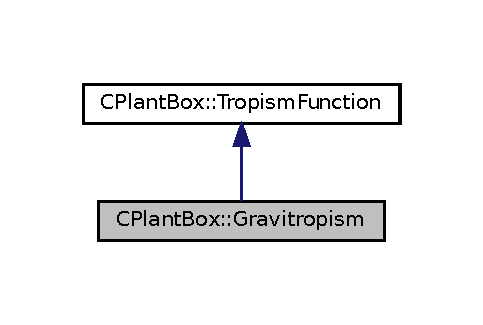
\includegraphics[width=232pt]{classCPlantBox_1_1Gravitropism__inherit__graph}
\end{center}
\end{figure}


Collaboration diagram for C\+Plant\+Box\+:\+:Gravitropism\+:\nopagebreak
\begin{figure}[H]
\begin{center}
\leavevmode
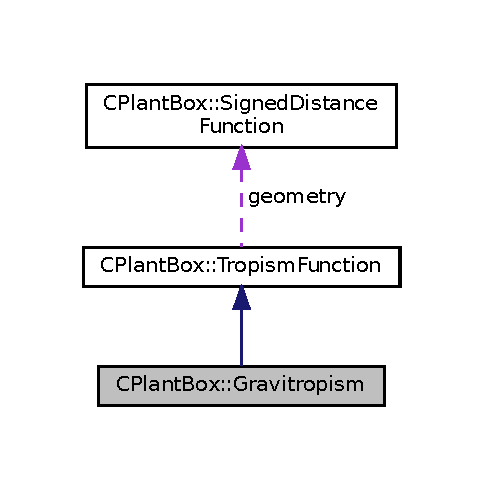
\includegraphics[width=232pt]{classCPlantBox_1_1Gravitropism__coll__graph}
\end{center}
\end{figure}
\subsection*{Public Member Functions}
\begin{DoxyCompactItemize}
\item 
\hyperlink{classCPlantBox_1_1Gravitropism_a2a6a57c372c3257e72156160c8fc5e6b}{Gravitropism} (double \hyperlink{classCPlantBox_1_1TropismFunction_a619c74d63319c406730c95679784a04a}{n}, double \hyperlink{classCPlantBox_1_1TropismFunction_acdc5f9c3beda0a74ddadd591c5d8afaf}{sigma})
\item 
\mbox{\Hypertarget{classCPlantBox_1_1Gravitropism_a210a09ce5911d8e58270e81d3d41a1e3}\label{classCPlantBox_1_1Gravitropism_a210a09ce5911d8e58270e81d3d41a1e3}} 
virtual \hyperlink{classCPlantBox_1_1TropismFunction}{Tropism\+Function} $\ast$ \hyperlink{classCPlantBox_1_1Gravitropism_a210a09ce5911d8e58270e81d3d41a1e3}{copy} () override
\begin{DoxyCompactList}\small\item\em copy constructor \end{DoxyCompactList}\item 
virtual double \hyperlink{classCPlantBox_1_1Gravitropism_a4471a30549db829fe19a91650ca8f87e}{tropism\+Objective} (const \hyperlink{classCPlantBox_1_1Vector3d}{Vector3d} \&pos, \hyperlink{classCPlantBox_1_1Matrix3d}{Matrix3d} old, double a, double b, double dx, const \hyperlink{classCPlantBox_1_1Organ}{Organ} $\ast$root) override
\begin{DoxyCompactList}\small\item\em \hyperlink{classCPlantBox_1_1TropismFunction_adb52b88734a94fe1365a00e02c7e6be5}{Tropism\+Function\+::get\+Heading} minimizes this function,. \end{DoxyCompactList}\end{DoxyCompactItemize}
\subsection*{Additional Inherited Members}


\subsection{Detailed Description}
\hyperlink{classCPlantBox_1_1Gravitropism}{Gravitropism}\+: the tendency to grow downwards 

\subsection{Constructor \& Destructor Documentation}
\mbox{\Hypertarget{classCPlantBox_1_1Gravitropism_a2a6a57c372c3257e72156160c8fc5e6b}\label{classCPlantBox_1_1Gravitropism_a2a6a57c372c3257e72156160c8fc5e6b}} 
\index{C\+Plant\+Box\+::\+Gravitropism@{C\+Plant\+Box\+::\+Gravitropism}!Gravitropism@{Gravitropism}}
\index{Gravitropism@{Gravitropism}!C\+Plant\+Box\+::\+Gravitropism@{C\+Plant\+Box\+::\+Gravitropism}}
\subsubsection{\texorpdfstring{Gravitropism()}{Gravitropism()}}
{\footnotesize\ttfamily C\+Plant\+Box\+::\+Gravitropism\+::\+Gravitropism (\begin{DoxyParamCaption}\item[{double}]{n,  }\item[{double}]{sigma }\end{DoxyParamCaption})\hspace{0.3cm}{\ttfamily [inline]}}

\begin{DoxySeeAlso}{See also}
\hyperlink{classCPlantBox_1_1TropismFunction}{Tropism\+Function} 
\end{DoxySeeAlso}


\subsection{Member Function Documentation}
\mbox{\Hypertarget{classCPlantBox_1_1Gravitropism_a4471a30549db829fe19a91650ca8f87e}\label{classCPlantBox_1_1Gravitropism_a4471a30549db829fe19a91650ca8f87e}} 
\index{C\+Plant\+Box\+::\+Gravitropism@{C\+Plant\+Box\+::\+Gravitropism}!tropism\+Objective@{tropism\+Objective}}
\index{tropism\+Objective@{tropism\+Objective}!C\+Plant\+Box\+::\+Gravitropism@{C\+Plant\+Box\+::\+Gravitropism}}
\subsubsection{\texorpdfstring{tropism\+Objective()}{tropismObjective()}}
{\footnotesize\ttfamily virtual double C\+Plant\+Box\+::\+Gravitropism\+::tropism\+Objective (\begin{DoxyParamCaption}\item[{const \hyperlink{classCPlantBox_1_1Vector3d}{Vector3d} \&}]{pos,  }\item[{\hyperlink{classCPlantBox_1_1Matrix3d}{Matrix3d}}]{old,  }\item[{double}]{a,  }\item[{double}]{b,  }\item[{double}]{dx,  }\item[{const \hyperlink{classCPlantBox_1_1Organ}{Organ} $\ast$}]{root }\end{DoxyParamCaption})\hspace{0.3cm}{\ttfamily [inline]}, {\ttfamily [override]}, {\ttfamily [virtual]}}



\hyperlink{classCPlantBox_1_1TropismFunction_adb52b88734a94fe1365a00e02c7e6be5}{Tropism\+Function\+::get\+Heading} minimizes this function,. 

\begin{DoxySeeAlso}{See also}
\hyperlink{classCPlantBox_1_1TropismFunction_adb52b88734a94fe1365a00e02c7e6be5}{Tropism\+Function\+::get\+Heading} and 

\hyperlink{classCPlantBox_1_1TropismFunction_a4f2c79fff55d1398c98a070dd8ebbe08}{Tropism\+Function\+::tropism\+Objective} 
\end{DoxySeeAlso}


Reimplemented from \hyperlink{classCPlantBox_1_1TropismFunction_a4f2c79fff55d1398c98a070dd8ebbe08}{C\+Plant\+Box\+::\+Tropism\+Function}.



The documentation for this class was generated from the following file\+:\begin{DoxyCompactItemize}
\item 
src/Root\+Tropism.\+h\end{DoxyCompactItemize}

\hypertarget{classCPlantBox_1_1GrowthFunction}{}\section{C\+Plant\+Box\+:\+:Growth\+Function Class Reference}
\label{classCPlantBox_1_1GrowthFunction}\index{C\+Plant\+Box\+::\+Growth\+Function@{C\+Plant\+Box\+::\+Growth\+Function}}


{\ttfamily \#include $<$Root\+Growth.\+h$>$}



Inheritance diagram for C\+Plant\+Box\+:\+:Growth\+Function\+:\nopagebreak
\begin{figure}[H]
\begin{center}
\leavevmode
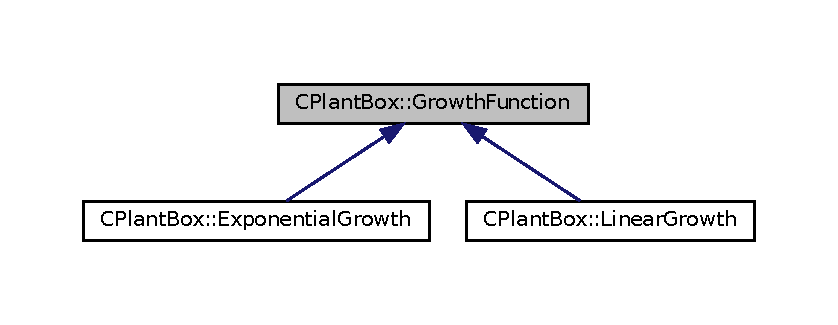
\includegraphics[width=350pt]{classCPlantBox_1_1GrowthFunction__inherit__graph}
\end{center}
\end{figure}
\subsection*{Public Member Functions}
\begin{DoxyCompactItemize}
\item 
virtual double \hyperlink{classCPlantBox_1_1GrowthFunction_a41b83da5d75beab49846c5b92a421e43}{get\+Length} (double t, double r, double k, \hyperlink{classCPlantBox_1_1Organ}{Organ} $\ast$root) const
\begin{DoxyCompactList}\small\item\em Returns root length at root age t. \end{DoxyCompactList}\item 
virtual double \hyperlink{classCPlantBox_1_1GrowthFunction_a006b428760c410389afa54853fe7cc1f}{get\+Age} (double l, double r, double k, \hyperlink{classCPlantBox_1_1Organ}{Organ} $\ast$root) const
\begin{DoxyCompactList}\small\item\em Returns the age of a root of length l. \end{DoxyCompactList}\end{DoxyCompactItemize}


\subsection{Detailed Description}
Abstract base class to all growth functions\+: currently \hyperlink{classCPlantBox_1_1LinearGrowth}{Linear\+Growth} and \hyperlink{classCPlantBox_1_1ExponentialGrowth}{Exponential\+Growth}

If new classes are created, they have to be added to the vector gf in in Root\+System. 

\subsection{Member Function Documentation}
\mbox{\Hypertarget{classCPlantBox_1_1GrowthFunction_a006b428760c410389afa54853fe7cc1f}\label{classCPlantBox_1_1GrowthFunction_a006b428760c410389afa54853fe7cc1f}} 
\index{C\+Plant\+Box\+::\+Growth\+Function@{C\+Plant\+Box\+::\+Growth\+Function}!get\+Age@{get\+Age}}
\index{get\+Age@{get\+Age}!C\+Plant\+Box\+::\+Growth\+Function@{C\+Plant\+Box\+::\+Growth\+Function}}
\subsubsection{\texorpdfstring{get\+Age()}{getAge()}}
{\footnotesize\ttfamily virtual double C\+Plant\+Box\+::\+Growth\+Function\+::get\+Age (\begin{DoxyParamCaption}\item[{double}]{l,  }\item[{double}]{r,  }\item[{double}]{k,  }\item[{\hyperlink{classCPlantBox_1_1Organ}{Organ} $\ast$}]{root }\end{DoxyParamCaption}) const\hspace{0.3cm}{\ttfamily [inline]}, {\ttfamily [virtual]}}



Returns the age of a root of length l. 

Returns the age of a root of length l


\begin{DoxyParams}{Parameters}
{\em l} & root length \mbox{[}cm\mbox{]} \\
\hline
{\em r} & initial growth rate \mbox{[}cm/day\mbox{]} \\
\hline
{\em k} & maximal root length \mbox{[}cm\mbox{]} \\
\hline
{\em root} & points to the root in case more information is needed\\
\hline
\end{DoxyParams}
\begin{DoxyReturn}{Returns}
root age \mbox{[}day\mbox{]} 
\end{DoxyReturn}


Reimplemented in \hyperlink{classCPlantBox_1_1ExponentialGrowth_af3fd28ae8c778bc823fc0e51756e8b63}{C\+Plant\+Box\+::\+Exponential\+Growth}, and \hyperlink{classCPlantBox_1_1LinearGrowth_a7880e35aa61d276647d9a602775dd87a}{C\+Plant\+Box\+::\+Linear\+Growth}.

\mbox{\Hypertarget{classCPlantBox_1_1GrowthFunction_a41b83da5d75beab49846c5b92a421e43}\label{classCPlantBox_1_1GrowthFunction_a41b83da5d75beab49846c5b92a421e43}} 
\index{C\+Plant\+Box\+::\+Growth\+Function@{C\+Plant\+Box\+::\+Growth\+Function}!get\+Length@{get\+Length}}
\index{get\+Length@{get\+Length}!C\+Plant\+Box\+::\+Growth\+Function@{C\+Plant\+Box\+::\+Growth\+Function}}
\subsubsection{\texorpdfstring{get\+Length()}{getLength()}}
{\footnotesize\ttfamily virtual double C\+Plant\+Box\+::\+Growth\+Function\+::get\+Length (\begin{DoxyParamCaption}\item[{double}]{t,  }\item[{double}]{r,  }\item[{double}]{k,  }\item[{\hyperlink{classCPlantBox_1_1Organ}{Organ} $\ast$}]{root }\end{DoxyParamCaption}) const\hspace{0.3cm}{\ttfamily [inline]}, {\ttfamily [virtual]}}



Returns root length at root age t. 

Returns root length at root age t


\begin{DoxyParams}{Parameters}
{\em t} & root age \mbox{[}day\mbox{]} \\
\hline
{\em r} & initial growth rate \mbox{[}cm/day\mbox{]} \\
\hline
{\em k} & maximal root length \mbox{[}cm\mbox{]} \\
\hline
{\em root} & points to the root in case more information is needed\\
\hline
\end{DoxyParams}
\begin{DoxyReturn}{Returns}
root length \mbox{[}cm\mbox{]} 
\end{DoxyReturn}


Reimplemented in \hyperlink{classCPlantBox_1_1ExponentialGrowth_ae5b0f12177b71c66d199fa515698aefa}{C\+Plant\+Box\+::\+Exponential\+Growth}, and \hyperlink{classCPlantBox_1_1LinearGrowth_afffda4dacad7cd28f6addb6d3268cf1f}{C\+Plant\+Box\+::\+Linear\+Growth}.



The documentation for this class was generated from the following file\+:\begin{DoxyCompactItemize}
\item 
src/Root\+Growth.\+h\end{DoxyCompactItemize}

\hypertarget{classCPlantBox_1_1Hydrotropism}{}\section{C\+Plant\+Box\+:\+:Hydrotropism Class Reference}
\label{classCPlantBox_1_1Hydrotropism}\index{C\+Plant\+Box\+::\+Hydrotropism@{C\+Plant\+Box\+::\+Hydrotropism}}


{\ttfamily \#include $<$Root\+Tropism.\+h$>$}



Inheritance diagram for C\+Plant\+Box\+:\+:Hydrotropism\+:\nopagebreak
\begin{figure}[H]
\begin{center}
\leavevmode
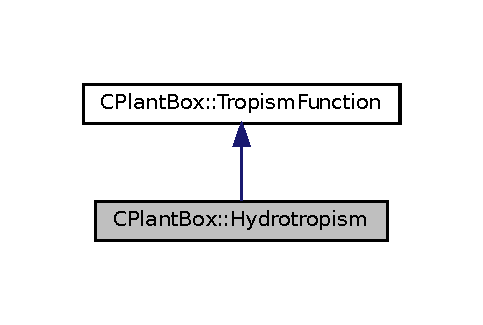
\includegraphics[width=232pt]{classCPlantBox_1_1Hydrotropism__inherit__graph}
\end{center}
\end{figure}


Collaboration diagram for C\+Plant\+Box\+:\+:Hydrotropism\+:\nopagebreak
\begin{figure}[H]
\begin{center}
\leavevmode
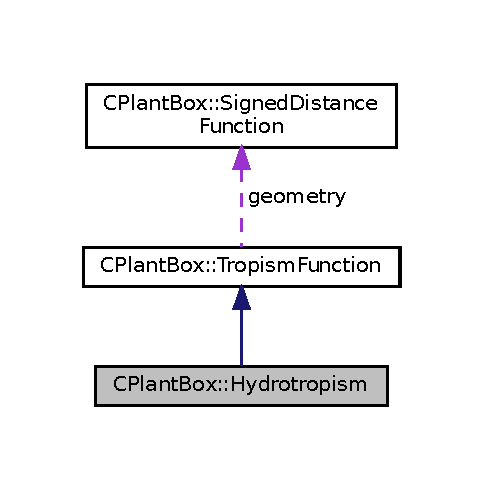
\includegraphics[width=232pt]{classCPlantBox_1_1Hydrotropism__coll__graph}
\end{center}
\end{figure}
\subsection*{Public Member Functions}
\begin{DoxyCompactItemize}
\item 
\hyperlink{classCPlantBox_1_1Hydrotropism_a7ffb4286e84c0d1b06374b43ceb29848}{Hydrotropism} (double \hyperlink{classCPlantBox_1_1TropismFunction_a619c74d63319c406730c95679784a04a}{n}, double \hyperlink{classCPlantBox_1_1TropismFunction_acdc5f9c3beda0a74ddadd591c5d8afaf}{sigma}, \hyperlink{classCPlantBox_1_1SoilLookUp}{Soil\+Look\+Up} $\ast$soil)
\item 
\mbox{\Hypertarget{classCPlantBox_1_1Hydrotropism_abf5359dcc5966638e89c802dd49a47bb}\label{classCPlantBox_1_1Hydrotropism_abf5359dcc5966638e89c802dd49a47bb}} 
virtual \hyperlink{classCPlantBox_1_1TropismFunction}{Tropism\+Function} $\ast$ \hyperlink{classCPlantBox_1_1Hydrotropism_abf5359dcc5966638e89c802dd49a47bb}{copy} () override
\begin{DoxyCompactList}\small\item\em copy constructor \end{DoxyCompactList}\item 
virtual double \hyperlink{classCPlantBox_1_1Hydrotropism_a5f259c82922f6d62df17f07827db0338}{tropism\+Objective} (const \hyperlink{classCPlantBox_1_1Vector3d}{Vector3d} \&pos, \hyperlink{classCPlantBox_1_1Matrix3d}{Matrix3d} old, double a, double b, double dx, const \hyperlink{classCPlantBox_1_1Organ}{Organ} $\ast$root) override
\begin{DoxyCompactList}\small\item\em \hyperlink{classCPlantBox_1_1TropismFunction_adb52b88734a94fe1365a00e02c7e6be5}{get\+Heading()} minimizes this function, \end{DoxyCompactList}\end{DoxyCompactItemize}
\subsection*{Additional Inherited Members}


\subsection{Detailed Description}
\hyperlink{classCPlantBox_1_1Hydrotropism}{Hydrotropism} (or Chemotropism, ...)\+: the tendency to grow towards a higher saturation (or concentration, ...) 

\subsection{Constructor \& Destructor Documentation}
\mbox{\Hypertarget{classCPlantBox_1_1Hydrotropism_a7ffb4286e84c0d1b06374b43ceb29848}\label{classCPlantBox_1_1Hydrotropism_a7ffb4286e84c0d1b06374b43ceb29848}} 
\index{C\+Plant\+Box\+::\+Hydrotropism@{C\+Plant\+Box\+::\+Hydrotropism}!Hydrotropism@{Hydrotropism}}
\index{Hydrotropism@{Hydrotropism}!C\+Plant\+Box\+::\+Hydrotropism@{C\+Plant\+Box\+::\+Hydrotropism}}
\subsubsection{\texorpdfstring{Hydrotropism()}{Hydrotropism()}}
{\footnotesize\ttfamily C\+Plant\+Box\+::\+Hydrotropism\+::\+Hydrotropism (\begin{DoxyParamCaption}\item[{double}]{n,  }\item[{double}]{sigma,  }\item[{\hyperlink{classCPlantBox_1_1SoilLookUp}{Soil\+Look\+Up} $\ast$}]{soil }\end{DoxyParamCaption})\hspace{0.3cm}{\ttfamily [inline]}}

\begin{DoxySeeAlso}{See also}
\hyperlink{classCPlantBox_1_1TropismFunction}{Tropism\+Function} 
\end{DoxySeeAlso}


\subsection{Member Function Documentation}
\mbox{\Hypertarget{classCPlantBox_1_1Hydrotropism_a5f259c82922f6d62df17f07827db0338}\label{classCPlantBox_1_1Hydrotropism_a5f259c82922f6d62df17f07827db0338}} 
\index{C\+Plant\+Box\+::\+Hydrotropism@{C\+Plant\+Box\+::\+Hydrotropism}!tropism\+Objective@{tropism\+Objective}}
\index{tropism\+Objective@{tropism\+Objective}!C\+Plant\+Box\+::\+Hydrotropism@{C\+Plant\+Box\+::\+Hydrotropism}}
\subsubsection{\texorpdfstring{tropism\+Objective()}{tropismObjective()}}
{\footnotesize\ttfamily double C\+Plant\+Box\+::\+Hydrotropism\+::tropism\+Objective (\begin{DoxyParamCaption}\item[{const \hyperlink{classCPlantBox_1_1Vector3d}{Vector3d} \&}]{pos,  }\item[{\hyperlink{classCPlantBox_1_1Matrix3d}{Matrix3d}}]{old,  }\item[{double}]{a,  }\item[{double}]{b,  }\item[{double}]{dx,  }\item[{const \hyperlink{classCPlantBox_1_1Organ}{Organ} $\ast$}]{root }\end{DoxyParamCaption})\hspace{0.3cm}{\ttfamily [override]}, {\ttfamily [virtual]}}



\hyperlink{classCPlantBox_1_1TropismFunction_adb52b88734a94fe1365a00e02c7e6be5}{get\+Heading()} minimizes this function, 

\begin{DoxySeeAlso}{See also}
\hyperlink{classCPlantBox_1_1TropismFunction}{Tropism\+Function}
\end{DoxySeeAlso}
\hyperlink{classCPlantBox_1_1TropismFunction_adb52b88734a94fe1365a00e02c7e6be5}{get\+Heading()} minimizes this function, \begin{DoxySeeAlso}{See also}
\hyperlink{classCPlantBox_1_1TropismFunction_a4f2c79fff55d1398c98a070dd8ebbe08}{Tropism\+Function\+::tropism\+Objective} 
\end{DoxySeeAlso}
$<$ (-\/1) because we want to maximize the soil property 

Reimplemented from \hyperlink{classCPlantBox_1_1TropismFunction_a4f2c79fff55d1398c98a070dd8ebbe08}{C\+Plant\+Box\+::\+Tropism\+Function}.



The documentation for this class was generated from the following files\+:\begin{DoxyCompactItemize}
\item 
src/Root\+Tropism.\+h\item 
src/Root\+Tropism.\+cpp\end{DoxyCompactItemize}

\hypertarget{classCPlantBox_1_1Leaf}{}\section{C\+Plant\+Box\+:\+:Leaf Class Reference}
\label{classCPlantBox_1_1Leaf}\index{C\+Plant\+Box\+::\+Leaf@{C\+Plant\+Box\+::\+Leaf}}


{\ttfamily \#include $<$Leaf.\+h$>$}



Inheritance diagram for C\+Plant\+Box\+:\+:Leaf\+:\nopagebreak
\begin{figure}[H]
\begin{center}
\leavevmode
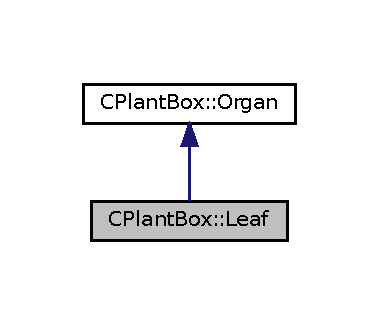
\includegraphics[width=182pt]{classCPlantBox_1_1Leaf__inherit__graph}
\end{center}
\end{figure}


Collaboration diagram for C\+Plant\+Box\+:\+:Leaf\+:\nopagebreak
\begin{figure}[H]
\begin{center}
\leavevmode
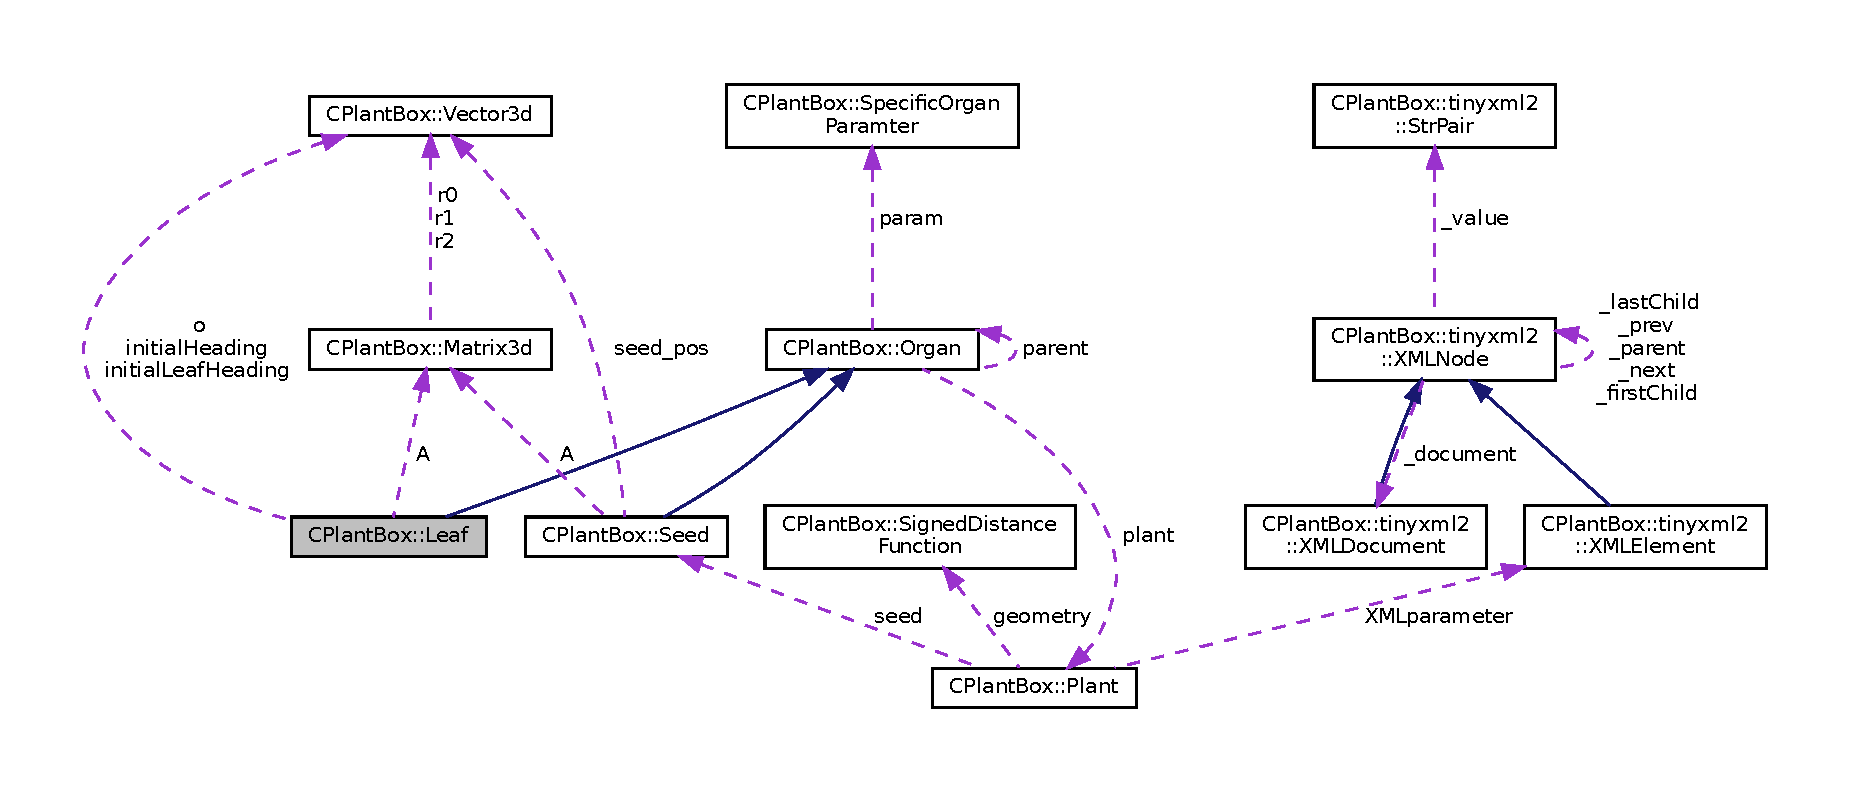
\includegraphics[width=350pt]{classCPlantBox_1_1Leaf__coll__graph}
\end{center}
\end{figure}
\subsection*{Public Member Functions}
\begin{DoxyCompactItemize}
\item 
\hyperlink{classCPlantBox_1_1Leaf_a00707cb127c0c09df6b63a5be0d3a35e}{Leaf} (\hyperlink{classCPlantBox_1_1Plant}{Plant} $\ast$\hyperlink{classCPlantBox_1_1Organ_ac614456886ab270c6fd2617403e0f306}{plant}, \hyperlink{classCPlantBox_1_1Organ}{Organ} $\ast$\hyperlink{classCPlantBox_1_1Organ_a8ad90078d5ef859bd2ab71700854e286}{parent}, int subtype, double delay, \hyperlink{classCPlantBox_1_1Vector3d}{Vector3d} ilheading, int \hyperlink{classCPlantBox_1_1Leaf_a533cb09f68a86c55321b2b28e3f8085a}{pni}, double \hyperlink{classCPlantBox_1_1Leaf_a7c503767ee8008fb9555f1f4590435c5}{pbl})
\begin{DoxyCompactList}\small\item\em typically called by constructor of Plant\+::\+Plant, or Leaf\+::create\+Laterals() \end{DoxyCompactList}\item 
\mbox{\Hypertarget{classCPlantBox_1_1Leaf_af7556eb19d907b277e314e09dce849de}\label{classCPlantBox_1_1Leaf_af7556eb19d907b277e314e09dce849de}} 
virtual int \hyperlink{classCPlantBox_1_1Leaf_af7556eb19d907b277e314e09dce849de}{organ\+Type} () const override
\begin{DoxyCompactList}\small\item\em returns the organs type, overwrite for each organ \end{DoxyCompactList}\item 
virtual void \hyperlink{classCPlantBox_1_1Leaf_ac8f35a92020107f44059b995e44af5d6}{simulate} (double dt, bool silence=false) override
\begin{DoxyCompactList}\small\item\em stem growth for a time span of \end{DoxyCompactList}\item 
\mbox{\Hypertarget{classCPlantBox_1_1Leaf_a97bb6cc92a59f0d137eb6b497b5d376e}\label{classCPlantBox_1_1Leaf_a97bb6cc92a59f0d137eb6b497b5d376e}} 
virtual double \hyperlink{classCPlantBox_1_1Leaf_a97bb6cc92a59f0d137eb6b497b5d376e}{get\+Scalar} (std\+::string name) const override
\begin{DoxyCompactList}\small\item\em returns an organ parameter of Plant\+::\+Scalar\+Type \end{DoxyCompactList}\item 
double \hyperlink{classCPlantBox_1_1Leaf_afe95477ee2292326a11b2844ca336229}{get\+Creation\+Time} (double lenght)
\begin{DoxyCompactList}\small\item\em analytical creation (=emergence) time of a node at a length \end{DoxyCompactList}\item 
double \hyperlink{classCPlantBox_1_1Leaf_a7056b1a0b28172daa7ce5e69b2f6c435}{Leaf\+Get\+Length} (double \hyperlink{classCPlantBox_1_1Organ_a4f17f0bfe7f03eedf4138fd8fe51376d}{age})
\begin{DoxyCompactList}\small\item\em analytical length of the stem \end{DoxyCompactList}\item 
double \hyperlink{classCPlantBox_1_1Leaf_a9939b2ee6247b9354dbe6d6c16d3442e}{Leaf\+Get\+Age} (double \hyperlink{classCPlantBox_1_1Organ_a94f5b16aa7ebc3912501051281fe88dc}{length})
\begin{DoxyCompactList}\small\item\em analytical age of the stem \end{DoxyCompactList}\item 
\mbox{\Hypertarget{classCPlantBox_1_1Leaf_aa9161845b757757d56aebad1abe293fd}\label{classCPlantBox_1_1Leaf_aa9161845b757757d56aebad1abe293fd}} 
\hyperlink{classCPlantBox_1_1LeafParameter}{Leaf\+Parameter} $\ast$ \hyperlink{classCPlantBox_1_1Leaf_aa9161845b757757d56aebad1abe293fd}{l\+Param} () const
\begin{DoxyCompactList}\small\item\em type cast \end{DoxyCompactList}\item 
\mbox{\Hypertarget{classCPlantBox_1_1Leaf_a91f9c3be23a6fd3d2c9b5438fc74e0fa}\label{classCPlantBox_1_1Leaf_a91f9c3be23a6fd3d2c9b5438fc74e0fa}} 
\hyperlink{classCPlantBox_1_1LeafRandomOrganParameter}{Leaf\+Random\+Organ\+Parameter} $\ast$ {\bfseries lt\+Param} () const
\item 
\mbox{\Hypertarget{classCPlantBox_1_1Leaf_a9999dbde2459edd66dc2a9c2d262c11e}\label{classCPlantBox_1_1Leaf_a9999dbde2459edd66dc2a9c2d262c11e}} 
double \hyperlink{classCPlantBox_1_1Leaf_a9999dbde2459edd66dc2a9c2d262c11e}{dx} () const
\begin{DoxyCompactList}\small\item\em returns the axial resolution \end{DoxyCompactList}\item 
\mbox{\Hypertarget{classCPlantBox_1_1Leaf_ae68f299d352c727ff048406ac4d20533}\label{classCPlantBox_1_1Leaf_ae68f299d352c727ff048406ac4d20533}} 
std\+::string {\bfseries name} () const
\item 
\hyperlink{classCPlantBox_1_1Vector3d}{Vector3d} \hyperlink{classCPlantBox_1_1Leaf_a89394580667c92220d87eae287faf5a9}{heading} () const
\item 
void \hyperlink{classCPlantBox_1_1Leaf_a0b5fbb524de825790da55551a212d4a0}{write\+R\+S\+ML} (std\+::ostream \&cout, std\+::string indent) const
\begin{DoxyCompactList}\small\item\em current heading of the root tip \end{DoxyCompactList}\item 
std\+::string \hyperlink{classCPlantBox_1_1Leaf_a7c09270825fa8f874dcf409969dbb554}{to\+String} () const
\item 
void \hyperlink{classCPlantBox_1_1Leaf_a9f4d6290903936f87fb016d8e0bbe344}{add\+Node} (\hyperlink{classCPlantBox_1_1Vector3d}{Vector3d} n, double t)
\item 
\mbox{\Hypertarget{classCPlantBox_1_1Leaf_a755a8ce67ead658bc329de33c404ed82}\label{classCPlantBox_1_1Leaf_a755a8ce67ead658bc329de33c404ed82}} 
virtual void \hyperlink{classCPlantBox_1_1Leaf_a755a8ce67ead658bc329de33c404ed82}{set\+Relative\+Origin} (const \hyperlink{classCPlantBox_1_1Vector3d}{Vector3d} \&o) override
\begin{DoxyCompactList}\small\item\em the relative position within the parent organ \end{DoxyCompactList}\item 
\mbox{\Hypertarget{classCPlantBox_1_1Leaf_abfe0297a2b109a82f21224aeae1e50e0}\label{classCPlantBox_1_1Leaf_abfe0297a2b109a82f21224aeae1e50e0}} 
virtual \hyperlink{classCPlantBox_1_1Vector3d}{Vector3d} {\bfseries get\+Relative\+Origin} () const override
\item 
\mbox{\Hypertarget{classCPlantBox_1_1Leaf_afb6a3c04e1197a510617574bc72e8a47}\label{classCPlantBox_1_1Leaf_afb6a3c04e1197a510617574bc72e8a47}} 
virtual void \hyperlink{classCPlantBox_1_1Leaf_afb6a3c04e1197a510617574bc72e8a47}{set\+Relative\+Heading} (const \hyperlink{classCPlantBox_1_1Matrix3d}{Matrix3d} \&m) override
\begin{DoxyCompactList}\small\item\em the heading in the parent organ \end{DoxyCompactList}\item 
\mbox{\Hypertarget{classCPlantBox_1_1Leaf_a93286071bb116459962e9b0365ed5001}\label{classCPlantBox_1_1Leaf_a93286071bb116459962e9b0365ed5001}} 
virtual \hyperlink{classCPlantBox_1_1Matrix3d}{Matrix3d} \hyperlink{classCPlantBox_1_1Leaf_a93286071bb116459962e9b0365ed5001}{get\+Relative\+Heading} () const override
\begin{DoxyCompactList}\small\item\em the relative position within the parent organ \end{DoxyCompactList}\item 
void \hyperlink{classCPlantBox_1_1Leaf_a8778214ada72f26a9e9e71dcd8cac087}{create\+Lateral} (bool silence)
\begin{DoxyCompactList}\small\item\em creates a new lateral, called by \hyperlink{classCPlantBox_1_1Leaf_ac8f35a92020107f44059b995e44af5d6}{Leaf\+::simulate()} \end{DoxyCompactList}\item 
\mbox{\Hypertarget{classCPlantBox_1_1Leaf_ae05cf8384ee6186d728c2c1fe9a7db67}\label{classCPlantBox_1_1Leaf_ae05cf8384ee6186d728c2c1fe9a7db67}} 
void {\bfseries minus\+Phytomer\+Id} (int subtype)
\item 
\mbox{\Hypertarget{classCPlantBox_1_1Leaf_acb5adec7a2e5088ca1150c821e765a9e}\label{classCPlantBox_1_1Leaf_acb5adec7a2e5088ca1150c821e765a9e}} 
int {\bfseries getleafphytomer\+ID} (int subtype)
\item 
\mbox{\Hypertarget{classCPlantBox_1_1Leaf_a5912cafb62d77befff4281f062a62b6c}\label{classCPlantBox_1_1Leaf_a5912cafb62d77befff4281f062a62b6c}} 
void {\bfseries addleafphytomer\+ID} (int subtype)
\end{DoxyCompactItemize}
\subsection*{Public Attributes}
\begin{DoxyCompactItemize}
\item 
\mbox{\Hypertarget{classCPlantBox_1_1Leaf_a911070d0046fbd3c9500154ab233fb46}\label{classCPlantBox_1_1Leaf_a911070d0046fbd3c9500154ab233fb46}} 
\hyperlink{classCPlantBox_1_1Vector3d}{Vector3d} {\bfseries initial\+Leaf\+Heading}
\item 
\mbox{\Hypertarget{classCPlantBox_1_1Leaf_a533cb09f68a86c55321b2b28e3f8085a}\label{classCPlantBox_1_1Leaf_a533cb09f68a86c55321b2b28e3f8085a}} 
int \hyperlink{classCPlantBox_1_1Leaf_a533cb09f68a86c55321b2b28e3f8085a}{pni}
\begin{DoxyCompactList}\small\item\em parent node index \end{DoxyCompactList}\item 
\mbox{\Hypertarget{classCPlantBox_1_1Leaf_a7c503767ee8008fb9555f1f4590435c5}\label{classCPlantBox_1_1Leaf_a7c503767ee8008fb9555f1f4590435c5}} 
double \hyperlink{classCPlantBox_1_1Leaf_a7c503767ee8008fb9555f1f4590435c5}{pbl}
\begin{DoxyCompactList}\small\item\em parent base length \mbox{[}cm\mbox{]} \end{DoxyCompactList}\item 
\mbox{\Hypertarget{classCPlantBox_1_1Leaf_a8771659afcda26d64e7e505a006790a3}\label{classCPlantBox_1_1Leaf_a8771659afcda26d64e7e505a006790a3}} 
const double \hyperlink{classCPlantBox_1_1Leaf_a8771659afcda26d64e7e505a006790a3}{small\+Dx} = 1e-\/6
\begin{DoxyCompactList}\small\item\em threshold value, smaller segments will be skipped (otherwise stem tip direction can become NaN) \end{DoxyCompactList}\item 
\mbox{\Hypertarget{classCPlantBox_1_1Leaf_ac7f33d0e34757c888521af4da83cffad}\label{classCPlantBox_1_1Leaf_ac7f33d0e34757c888521af4da83cffad}} 
\hyperlink{classCPlantBox_1_1Vector3d}{Vector3d} \hyperlink{classCPlantBox_1_1Leaf_ac7f33d0e34757c888521af4da83cffad}{initial\+Heading}
\begin{DoxyCompactList}\small\item\em a heading downward \end{DoxyCompactList}\item 
\mbox{\Hypertarget{classCPlantBox_1_1Leaf_a29ab9f0f1d359979004b9c3157061971}\label{classCPlantBox_1_1Leaf_a29ab9f0f1d359979004b9c3157061971}} 
double \hyperlink{classCPlantBox_1_1Leaf_a29ab9f0f1d359979004b9c3157061971}{parent\+\_\+base\+\_\+length}
\begin{DoxyCompactList}\small\item\em length \mbox{[}cm\mbox{]} \end{DoxyCompactList}\item 
\mbox{\Hypertarget{classCPlantBox_1_1Leaf_af8f3ec361de47481109ce9df93cda3ec}\label{classCPlantBox_1_1Leaf_af8f3ec361de47481109ce9df93cda3ec}} 
int \hyperlink{classCPlantBox_1_1Leaf_af8f3ec361de47481109ce9df93cda3ec}{parent\+\_\+ni}
\begin{DoxyCompactList}\small\item\em parent node index \end{DoxyCompactList}\item 
\mbox{\Hypertarget{classCPlantBox_1_1Leaf_abc6c84cb5ba202076261bcf1a308c7aa}\label{classCPlantBox_1_1Leaf_abc6c84cb5ba202076261bcf1a308c7aa}} 
\hyperlink{classCPlantBox_1_1Vector3d}{Vector3d} {\bfseries o}
\item 
\mbox{\Hypertarget{classCPlantBox_1_1Leaf_a98beba3528f76279c56152b171146a9b}\label{classCPlantBox_1_1Leaf_a98beba3528f76279c56152b171146a9b}} 
\hyperlink{classCPlantBox_1_1Matrix3d}{Matrix3d} {\bfseries A}
\end{DoxyCompactItemize}
\subsection*{Protected Member Functions}
\begin{DoxyCompactItemize}
\item 
void \hyperlink{classCPlantBox_1_1Leaf_ab41a29c6e050d8dd31690679e095b80e}{create\+Segments} (double l, bool silence)
\begin{DoxyCompactList}\small\item\em creates segments of length l, called by stem\+::simulate() \end{DoxyCompactList}\item 
\mbox{\Hypertarget{classCPlantBox_1_1Leaf_a8e9e823878a501b3703982b7679ef860}\label{classCPlantBox_1_1Leaf_a8e9e823878a501b3703982b7679ef860}} 
virtual \hyperlink{classCPlantBox_1_1Vector3d}{Vector3d} \hyperlink{classCPlantBox_1_1Leaf_a8e9e823878a501b3703982b7679ef860}{get\+Increment} (const \hyperlink{classCPlantBox_1_1Vector3d}{Vector3d} \&p, double sdx)
\begin{DoxyCompactList}\small\item\em called by create\+Segments, to determine growth direction \end{DoxyCompactList}\end{DoxyCompactItemize}
\subsection*{Protected Attributes}
\begin{DoxyCompactItemize}
\item 
\mbox{\Hypertarget{classCPlantBox_1_1Leaf_af1b6f6f42d3aa45710141e7f47124e6e}\label{classCPlantBox_1_1Leaf_af1b6f6f42d3aa45710141e7f47124e6e}} 
int {\bfseries old\+\_\+non} = 0
\end{DoxyCompactItemize}
\subsection*{Additional Inherited Members}


\subsection{Detailed Description}
\hyperlink{classCPlantBox_1_1Stem}{Stem}

Describes a single stem, by a vector of nodes representing the stem. The method \hyperlink{classCPlantBox_1_1Leaf_ac8f35a92020107f44059b995e44af5d6}{simulate()} creates new nodes of this stem, and lateral stems in the stem\textquotesingle{}s branching zone. 

\subsection{Constructor \& Destructor Documentation}
\mbox{\Hypertarget{classCPlantBox_1_1Leaf_a00707cb127c0c09df6b63a5be0d3a35e}\label{classCPlantBox_1_1Leaf_a00707cb127c0c09df6b63a5be0d3a35e}} 
\index{C\+Plant\+Box\+::\+Leaf@{C\+Plant\+Box\+::\+Leaf}!Leaf@{Leaf}}
\index{Leaf@{Leaf}!C\+Plant\+Box\+::\+Leaf@{C\+Plant\+Box\+::\+Leaf}}
\subsubsection{\texorpdfstring{Leaf()}{Leaf()}}
{\footnotesize\ttfamily C\+Plant\+Box\+::\+Leaf\+::\+Leaf (\begin{DoxyParamCaption}\item[{\hyperlink{classCPlantBox_1_1Plant}{Plant} $\ast$}]{plant,  }\item[{\hyperlink{classCPlantBox_1_1Organ}{Organ} $\ast$}]{parent,  }\item[{int}]{subtype,  }\item[{double}]{delay,  }\item[{\hyperlink{classCPlantBox_1_1Vector3d}{Vector3d}}]{ilheading,  }\item[{int}]{pni,  }\item[{double}]{pbl }\end{DoxyParamCaption})}



typically called by constructor of Plant\+::\+Plant, or Leaf\+::create\+Laterals() 

Constructor This is a Copy Paste of the Root.\+cpp but it works independently, it has its own parameter file (in .l\+Param file) tropism, growth function, txt and vtp writing syleaf. All of those can be modified to fit the real growth of the \hyperlink{classCPlantBox_1_1Plant}{Plant}.

Typically called by the Plant\+::\+Plant(), or Leaf\+::create\+New\+Leaf(). For leaf the initial node and node emergence time (netime) must be set from outside


\begin{DoxyParams}{Parameters}
{\em plant} & points to the plant \\
\hline
{\em parent} & points to the parent organ \\
\hline
{\em subtype} & sub type of the leaf \\
\hline
{\em delay} & delay after which the organ starts to develop (days) \\
\hline
{\em rheading} & relative heading (within parent organ) \\
\hline
{\em pni} & parent node index \\
\hline
{\em pbl} & parent base length \\
\hline
\end{DoxyParams}


\subsection{Member Function Documentation}
\mbox{\Hypertarget{classCPlantBox_1_1Leaf_a9f4d6290903936f87fb016d8e0bbe344}\label{classCPlantBox_1_1Leaf_a9f4d6290903936f87fb016d8e0bbe344}} 
\index{C\+Plant\+Box\+::\+Leaf@{C\+Plant\+Box\+::\+Leaf}!add\+Node@{add\+Node}}
\index{add\+Node@{add\+Node}!C\+Plant\+Box\+::\+Leaf@{C\+Plant\+Box\+::\+Leaf}}
\subsubsection{\texorpdfstring{add\+Node()}{addNode()}}
{\footnotesize\ttfamily void C\+Plant\+Box\+::\+Leaf\+::add\+Node (\begin{DoxyParamCaption}\item[{\hyperlink{classCPlantBox_1_1Vector3d}{Vector3d}}]{n,  }\item[{double}]{t }\end{DoxyParamCaption})}

Adds the next node to the leaf.

Add nodes only with this function! For simplicity nodes can not be deleted, and leafs can only become deactivated by dying


\begin{DoxyParams}{Parameters}
{\em n} & the new node \\
\hline
{\em t} & exact creation time of the node \\
\hline
\end{DoxyParams}
\mbox{\Hypertarget{classCPlantBox_1_1Leaf_a8778214ada72f26a9e9e71dcd8cac087}\label{classCPlantBox_1_1Leaf_a8778214ada72f26a9e9e71dcd8cac087}} 
\index{C\+Plant\+Box\+::\+Leaf@{C\+Plant\+Box\+::\+Leaf}!create\+Lateral@{create\+Lateral}}
\index{create\+Lateral@{create\+Lateral}!C\+Plant\+Box\+::\+Leaf@{C\+Plant\+Box\+::\+Leaf}}
\subsubsection{\texorpdfstring{create\+Lateral()}{createLateral()}}
{\footnotesize\ttfamily void C\+Plant\+Box\+::\+Leaf\+::create\+Lateral (\begin{DoxyParamCaption}\item[{bool}]{silence }\end{DoxyParamCaption})}



creates a new lateral, called by \hyperlink{classCPlantBox_1_1Leaf_ac8f35a92020107f44059b995e44af5d6}{Leaf\+::simulate()} 

Creates a new lateral by calling Leaf\+::create\+Newleaf().

Overwrite this method to implement more specialized leaf classes. \mbox{\Hypertarget{classCPlantBox_1_1Leaf_ab41a29c6e050d8dd31690679e095b80e}\label{classCPlantBox_1_1Leaf_ab41a29c6e050d8dd31690679e095b80e}} 
\index{C\+Plant\+Box\+::\+Leaf@{C\+Plant\+Box\+::\+Leaf}!create\+Segments@{create\+Segments}}
\index{create\+Segments@{create\+Segments}!C\+Plant\+Box\+::\+Leaf@{C\+Plant\+Box\+::\+Leaf}}
\subsubsection{\texorpdfstring{create\+Segments()}{createSegments()}}
{\footnotesize\ttfamily void C\+Plant\+Box\+::\+Leaf\+::create\+Segments (\begin{DoxyParamCaption}\item[{double}]{l,  }\item[{bool}]{silence }\end{DoxyParamCaption})\hspace{0.3cm}{\ttfamily [protected]}}



creates segments of length l, called by stem\+::simulate() 

Creates nodes and node emergence times for length l, and updates the leaf heading

Cecks that each new segments length is $<$= dx but $>$= ddx


\begin{DoxyParams}{Parameters}
{\em l} & length the leaf growth \mbox{[}cm\mbox{]} \\
\hline
\end{DoxyParams}
\mbox{\Hypertarget{classCPlantBox_1_1Leaf_afe95477ee2292326a11b2844ca336229}\label{classCPlantBox_1_1Leaf_afe95477ee2292326a11b2844ca336229}} 
\index{C\+Plant\+Box\+::\+Leaf@{C\+Plant\+Box\+::\+Leaf}!get\+Creation\+Time@{get\+Creation\+Time}}
\index{get\+Creation\+Time@{get\+Creation\+Time}!C\+Plant\+Box\+::\+Leaf@{C\+Plant\+Box\+::\+Leaf}}
\subsubsection{\texorpdfstring{get\+Creation\+Time()}{getCreationTime()}}
{\footnotesize\ttfamily double C\+Plant\+Box\+::\+Leaf\+::get\+Creation\+Time (\begin{DoxyParamCaption}\item[{double}]{length }\end{DoxyParamCaption})}



analytical creation (=emergence) time of a node at a length 

Analytical creation (=emergence) time of a node at a length along the leaf


\begin{DoxyParams}{Parameters}
{\em length} & length of the leaf \mbox{[}cm\mbox{]} \\
\hline
\end{DoxyParams}
\mbox{\Hypertarget{classCPlantBox_1_1Leaf_a89394580667c92220d87eae287faf5a9}\label{classCPlantBox_1_1Leaf_a89394580667c92220d87eae287faf5a9}} 
\index{C\+Plant\+Box\+::\+Leaf@{C\+Plant\+Box\+::\+Leaf}!heading@{heading}}
\index{heading@{heading}!C\+Plant\+Box\+::\+Leaf@{C\+Plant\+Box\+::\+Leaf}}
\subsubsection{\texorpdfstring{heading()}{heading()}}
{\footnotesize\ttfamily \hyperlink{classCPlantBox_1_1Vector3d}{Vector3d} C\+Plant\+Box\+::\+Leaf\+::heading (\begin{DoxyParamCaption}{ }\end{DoxyParamCaption}) const}

Relative heading of organ tip Absolute heading of organ tip \mbox{\Hypertarget{classCPlantBox_1_1Leaf_a9939b2ee6247b9354dbe6d6c16d3442e}\label{classCPlantBox_1_1Leaf_a9939b2ee6247b9354dbe6d6c16d3442e}} 
\index{C\+Plant\+Box\+::\+Leaf@{C\+Plant\+Box\+::\+Leaf}!Leaf\+Get\+Age@{Leaf\+Get\+Age}}
\index{Leaf\+Get\+Age@{Leaf\+Get\+Age}!C\+Plant\+Box\+::\+Leaf@{C\+Plant\+Box\+::\+Leaf}}
\subsubsection{\texorpdfstring{Leaf\+Get\+Age()}{LeafGetAge()}}
{\footnotesize\ttfamily double C\+Plant\+Box\+::\+Leaf\+::\+Leaf\+Get\+Age (\begin{DoxyParamCaption}\item[{double}]{length }\end{DoxyParamCaption})}



analytical age of the stem 

Analytical age of the leaf at a given length


\begin{DoxyParams}{Parameters}
{\em length} & length of the leaf \mbox{[}cm\mbox{]} \\
\hline
\end{DoxyParams}
\mbox{\Hypertarget{classCPlantBox_1_1Leaf_a7056b1a0b28172daa7ce5e69b2f6c435}\label{classCPlantBox_1_1Leaf_a7056b1a0b28172daa7ce5e69b2f6c435}} 
\index{C\+Plant\+Box\+::\+Leaf@{C\+Plant\+Box\+::\+Leaf}!Leaf\+Get\+Length@{Leaf\+Get\+Length}}
\index{Leaf\+Get\+Length@{Leaf\+Get\+Length}!C\+Plant\+Box\+::\+Leaf@{C\+Plant\+Box\+::\+Leaf}}
\subsubsection{\texorpdfstring{Leaf\+Get\+Length()}{LeafGetLength()}}
{\footnotesize\ttfamily double C\+Plant\+Box\+::\+Leaf\+::\+Leaf\+Get\+Length (\begin{DoxyParamCaption}\item[{double}]{age }\end{DoxyParamCaption})}



analytical length of the stem 

Analytical length of the leaf at a given age


\begin{DoxyParams}{Parameters}
{\em age} & age of the leaf \mbox{[}day\mbox{]} \\
\hline
\end{DoxyParams}
\mbox{\Hypertarget{classCPlantBox_1_1Leaf_ac8f35a92020107f44059b995e44af5d6}\label{classCPlantBox_1_1Leaf_ac8f35a92020107f44059b995e44af5d6}} 
\index{C\+Plant\+Box\+::\+Leaf@{C\+Plant\+Box\+::\+Leaf}!simulate@{simulate}}
\index{simulate@{simulate}!C\+Plant\+Box\+::\+Leaf@{C\+Plant\+Box\+::\+Leaf}}
\subsubsection{\texorpdfstring{simulate()}{simulate()}}
{\footnotesize\ttfamily void C\+Plant\+Box\+::\+Leaf\+::simulate (\begin{DoxyParamCaption}\item[{double}]{dt,  }\item[{bool}]{silence = {\ttfamily false} }\end{DoxyParamCaption})\hspace{0.3cm}{\ttfamily [override]}, {\ttfamily [virtual]}}



stem growth for a time span of 


\begin{DoxyParams}{Parameters}
{\em dt} & \\
\hline
\end{DoxyParams}
Simulates growth of this leaf for a time span dt


\begin{DoxyParams}{Parameters}
{\em dt} & time step \mbox{[}day\mbox{]} \\
\hline
{\em silence} & indicates if status messages are written to the console (cout) (default = false) \\
\hline
\end{DoxyParams}


Reimplemented from \hyperlink{classCPlantBox_1_1Organ_acf519fc6730c0adbb2a82b7702ff7a28}{C\+Plant\+Box\+::\+Organ}.

\mbox{\Hypertarget{classCPlantBox_1_1Leaf_a7c09270825fa8f874dcf409969dbb554}\label{classCPlantBox_1_1Leaf_a7c09270825fa8f874dcf409969dbb554}} 
\index{C\+Plant\+Box\+::\+Leaf@{C\+Plant\+Box\+::\+Leaf}!to\+String@{to\+String}}
\index{to\+String@{to\+String}!C\+Plant\+Box\+::\+Leaf@{C\+Plant\+Box\+::\+Leaf}}
\subsubsection{\texorpdfstring{to\+String()}{toString()}}
{\footnotesize\ttfamily std\+::string C\+Plant\+Box\+::\+Leaf\+::to\+String (\begin{DoxyParamCaption}{ }\end{DoxyParamCaption}) const\hspace{0.3cm}{\ttfamily [virtual]}}

Quick info about the object for debugging 

Reimplemented from \hyperlink{classCPlantBox_1_1Organ_a9f823aebd19519096e899e65604f239f}{C\+Plant\+Box\+::\+Organ}.

\mbox{\Hypertarget{classCPlantBox_1_1Leaf_a0b5fbb524de825790da55551a212d4a0}\label{classCPlantBox_1_1Leaf_a0b5fbb524de825790da55551a212d4a0}} 
\index{C\+Plant\+Box\+::\+Leaf@{C\+Plant\+Box\+::\+Leaf}!write\+R\+S\+ML@{write\+R\+S\+ML}}
\index{write\+R\+S\+ML@{write\+R\+S\+ML}!C\+Plant\+Box\+::\+Leaf@{C\+Plant\+Box\+::\+Leaf}}
\subsubsection{\texorpdfstring{write\+R\+S\+M\+L()}{writeRSML()}}
{\footnotesize\ttfamily void C\+Plant\+Box\+::\+Leaf\+::write\+R\+S\+ML (\begin{DoxyParamCaption}\item[{std\+::ostream \&}]{cout,  }\item[{std\+::string}]{indent }\end{DoxyParamCaption}) const\hspace{0.3cm}{\ttfamily [virtual]}}



current heading of the root tip 

writes a R\+S\+ML stem tag

writes R\+S\+ML leaf tag


\begin{DoxyParams}{Parameters}
{\em cout} & typically a file out stream \\
\hline
{\em indent} & we care for looks \\
\hline
\end{DoxyParams}


Reimplemented from \hyperlink{classCPlantBox_1_1Organ_acdad546c90e915b61ac3606f1f841ba1}{C\+Plant\+Box\+::\+Organ}.



The documentation for this class was generated from the following files\+:\begin{DoxyCompactItemize}
\item 
src/Leaf.\+h\item 
src/Leaf.\+cpp\end{DoxyCompactItemize}

\hypertarget{classCPlantBox_1_1LeafAntiGravitropism}{}\section{C\+Plant\+Box\+:\+:Leaf\+Anti\+Gravitropism Class Reference}
\label{classCPlantBox_1_1LeafAntiGravitropism}\index{C\+Plant\+Box\+::\+Leaf\+Anti\+Gravitropism@{C\+Plant\+Box\+::\+Leaf\+Anti\+Gravitropism}}


Inheritance diagram for C\+Plant\+Box\+:\+:Leaf\+Anti\+Gravitropism\+:\nopagebreak
\begin{figure}[H]
\begin{center}
\leavevmode
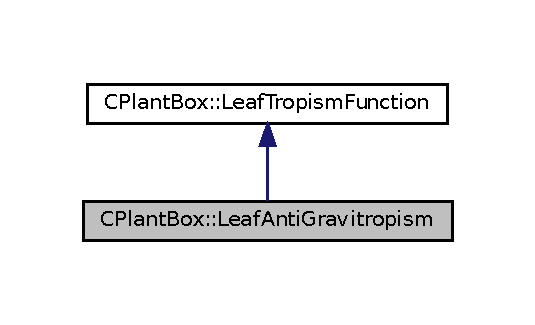
\includegraphics[width=257pt]{classCPlantBox_1_1LeafAntiGravitropism__inherit__graph}
\end{center}
\end{figure}


Collaboration diagram for C\+Plant\+Box\+:\+:Leaf\+Anti\+Gravitropism\+:\nopagebreak
\begin{figure}[H]
\begin{center}
\leavevmode
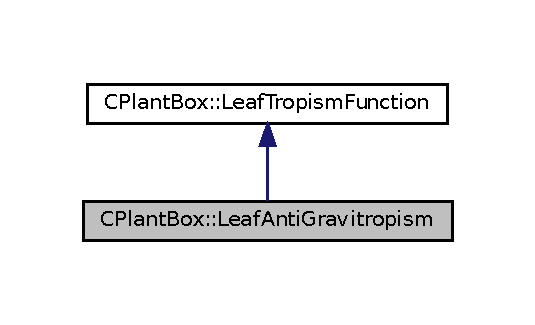
\includegraphics[width=257pt]{classCPlantBox_1_1LeafAntiGravitropism__coll__graph}
\end{center}
\end{figure}
\subsection*{Public Member Functions}
\begin{DoxyCompactItemize}
\item 
\hyperlink{classCPlantBox_1_1LeafAntiGravitropism_a3b2eb7861d5c9ffe4a57f7374dd6ebd5}{Leaf\+Anti\+Gravitropism} (double \hyperlink{classCPlantBox_1_1LeafTropismFunction_a21d8d756f8b9f6015b546def33b01c89}{n}, double \hyperlink{classCPlantBox_1_1LeafTropismFunction_a82a3dc11056a65501bc4535749c304b6}{sigma})
\item 
virtual double \hyperlink{classCPlantBox_1_1LeafAntiGravitropism_a94f4abfb99515326081deebff7906ca2}{leaftropism\+Objective} (const \hyperlink{classCPlantBox_1_1Vector3d}{Vector3d} \&pos, \hyperlink{classCPlantBox_1_1Matrix3d}{Matrix3d} old, double a, double b, double dx, const \hyperlink{classCPlantBox_1_1Organ}{Organ} $\ast$leaf) override
\begin{DoxyCompactList}\small\item\em \hyperlink{classCPlantBox_1_1TropismFunction_adb52b88734a94fe1365a00e02c7e6be5}{Tropism\+Function\+::get\+Heading} minimizes this function,. \end{DoxyCompactList}\end{DoxyCompactItemize}
\subsection*{Additional Inherited Members}


\subsection{Constructor \& Destructor Documentation}
\mbox{\Hypertarget{classCPlantBox_1_1LeafAntiGravitropism_a3b2eb7861d5c9ffe4a57f7374dd6ebd5}\label{classCPlantBox_1_1LeafAntiGravitropism_a3b2eb7861d5c9ffe4a57f7374dd6ebd5}} 
\index{C\+Plant\+Box\+::\+Leaf\+Anti\+Gravitropism@{C\+Plant\+Box\+::\+Leaf\+Anti\+Gravitropism}!Leaf\+Anti\+Gravitropism@{Leaf\+Anti\+Gravitropism}}
\index{Leaf\+Anti\+Gravitropism@{Leaf\+Anti\+Gravitropism}!C\+Plant\+Box\+::\+Leaf\+Anti\+Gravitropism@{C\+Plant\+Box\+::\+Leaf\+Anti\+Gravitropism}}
\subsubsection{\texorpdfstring{Leaf\+Anti\+Gravitropism()}{LeafAntiGravitropism()}}
{\footnotesize\ttfamily C\+Plant\+Box\+::\+Leaf\+Anti\+Gravitropism\+::\+Leaf\+Anti\+Gravitropism (\begin{DoxyParamCaption}\item[{double}]{n,  }\item[{double}]{sigma }\end{DoxyParamCaption})\hspace{0.3cm}{\ttfamily [inline]}}

\begin{DoxySeeAlso}{See also}
\hyperlink{classCPlantBox_1_1TropismFunction}{Tropism\+Function} 
\end{DoxySeeAlso}


\subsection{Member Function Documentation}
\mbox{\Hypertarget{classCPlantBox_1_1LeafAntiGravitropism_a94f4abfb99515326081deebff7906ca2}\label{classCPlantBox_1_1LeafAntiGravitropism_a94f4abfb99515326081deebff7906ca2}} 
\index{C\+Plant\+Box\+::\+Leaf\+Anti\+Gravitropism@{C\+Plant\+Box\+::\+Leaf\+Anti\+Gravitropism}!leaftropism\+Objective@{leaftropism\+Objective}}
\index{leaftropism\+Objective@{leaftropism\+Objective}!C\+Plant\+Box\+::\+Leaf\+Anti\+Gravitropism@{C\+Plant\+Box\+::\+Leaf\+Anti\+Gravitropism}}
\subsubsection{\texorpdfstring{leaftropism\+Objective()}{leaftropismObjective()}}
{\footnotesize\ttfamily virtual double C\+Plant\+Box\+::\+Leaf\+Anti\+Gravitropism\+::leaftropism\+Objective (\begin{DoxyParamCaption}\item[{const \hyperlink{classCPlantBox_1_1Vector3d}{Vector3d} \&}]{pos,  }\item[{\hyperlink{classCPlantBox_1_1Matrix3d}{Matrix3d}}]{old,  }\item[{double}]{a,  }\item[{double}]{b,  }\item[{double}]{dx,  }\item[{const \hyperlink{classCPlantBox_1_1Organ}{Organ} $\ast$}]{leaf }\end{DoxyParamCaption})\hspace{0.3cm}{\ttfamily [inline]}, {\ttfamily [override]}, {\ttfamily [virtual]}}



\hyperlink{classCPlantBox_1_1TropismFunction_adb52b88734a94fe1365a00e02c7e6be5}{Tropism\+Function\+::get\+Heading} minimizes this function,. 

\begin{DoxySeeAlso}{See also}
\hyperlink{classCPlantBox_1_1TropismFunction_adb52b88734a94fe1365a00e02c7e6be5}{Tropism\+Function\+::get\+Heading} and 

\hyperlink{classCPlantBox_1_1TropismFunction_a4f2c79fff55d1398c98a070dd8ebbe08}{Tropism\+Function\+::tropism\+Objective} 
\end{DoxySeeAlso}


Reimplemented from \hyperlink{classCPlantBox_1_1LeafTropismFunction_ab89f5f7e80103d80681bc8cadc220dba}{C\+Plant\+Box\+::\+Leaf\+Tropism\+Function}.



The documentation for this class was generated from the following file\+:\begin{DoxyCompactItemize}
\item 
src/Leaf\+Tropism.\+h\end{DoxyCompactItemize}

\hypertarget{classCPlantBox_1_1LeafExotropism}{}\section{C\+Plant\+Box\+:\+:Leaf\+Exotropism Class Reference}
\label{classCPlantBox_1_1LeafExotropism}\index{C\+Plant\+Box\+::\+Leaf\+Exotropism@{C\+Plant\+Box\+::\+Leaf\+Exotropism}}


{\ttfamily \#include $<$Leaf\+Tropism.\+h$>$}



Inheritance diagram for C\+Plant\+Box\+:\+:Leaf\+Exotropism\+:\nopagebreak
\begin{figure}[H]
\begin{center}
\leavevmode
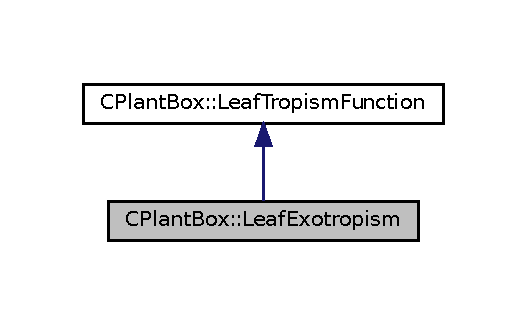
\includegraphics[width=253pt]{classCPlantBox_1_1LeafExotropism__inherit__graph}
\end{center}
\end{figure}


Collaboration diagram for C\+Plant\+Box\+:\+:Leaf\+Exotropism\+:\nopagebreak
\begin{figure}[H]
\begin{center}
\leavevmode
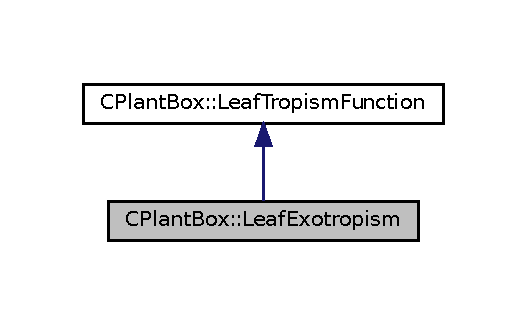
\includegraphics[width=253pt]{classCPlantBox_1_1LeafExotropism__coll__graph}
\end{center}
\end{figure}
\subsection*{Public Member Functions}
\begin{DoxyCompactItemize}
\item 
\hyperlink{classCPlantBox_1_1LeafExotropism_ad5e3bd8a6dcd60d33d31ed7df89a0078}{Leaf\+Exotropism} (double \hyperlink{classCPlantBox_1_1LeafTropismFunction_a21d8d756f8b9f6015b546def33b01c89}{n}, double \hyperlink{classCPlantBox_1_1LeafTropismFunction_a82a3dc11056a65501bc4535749c304b6}{sigma})
\item 
virtual double \hyperlink{classCPlantBox_1_1LeafExotropism_a0b3820189c2cef88d32a0d8130c15246}{leaftropism\+Objective} (const \hyperlink{classCPlantBox_1_1Vector3d}{Vector3d} \&pos, \hyperlink{classCPlantBox_1_1Matrix3d}{Matrix3d} old, double a, double b, double dx, const \hyperlink{classCPlantBox_1_1Organ}{Organ} $\ast$leaf) override
\begin{DoxyCompactList}\small\item\em \hyperlink{classCPlantBox_1_1LeafTropismFunction_a1440868221a834474e34e3a503a74572}{get\+Heading()} minimizes this function, \end{DoxyCompactList}\end{DoxyCompactItemize}
\subsection*{Additional Inherited Members}


\subsection{Detailed Description}
\hyperlink{classCPlantBox_1_1Exotropism}{Exotropism}\+: the tendency to keep the initial heading 

\subsection{Constructor \& Destructor Documentation}
\mbox{\Hypertarget{classCPlantBox_1_1LeafExotropism_ad5e3bd8a6dcd60d33d31ed7df89a0078}\label{classCPlantBox_1_1LeafExotropism_ad5e3bd8a6dcd60d33d31ed7df89a0078}} 
\index{C\+Plant\+Box\+::\+Leaf\+Exotropism@{C\+Plant\+Box\+::\+Leaf\+Exotropism}!Leaf\+Exotropism@{Leaf\+Exotropism}}
\index{Leaf\+Exotropism@{Leaf\+Exotropism}!C\+Plant\+Box\+::\+Leaf\+Exotropism@{C\+Plant\+Box\+::\+Leaf\+Exotropism}}
\subsubsection{\texorpdfstring{Leaf\+Exotropism()}{LeafExotropism()}}
{\footnotesize\ttfamily C\+Plant\+Box\+::\+Leaf\+Exotropism\+::\+Leaf\+Exotropism (\begin{DoxyParamCaption}\item[{double}]{n,  }\item[{double}]{sigma }\end{DoxyParamCaption})\hspace{0.3cm}{\ttfamily [inline]}}

\begin{DoxySeeAlso}{See also}
\hyperlink{classCPlantBox_1_1TropismFunction}{Tropism\+Function} 
\end{DoxySeeAlso}


\subsection{Member Function Documentation}
\mbox{\Hypertarget{classCPlantBox_1_1LeafExotropism_a0b3820189c2cef88d32a0d8130c15246}\label{classCPlantBox_1_1LeafExotropism_a0b3820189c2cef88d32a0d8130c15246}} 
\index{C\+Plant\+Box\+::\+Leaf\+Exotropism@{C\+Plant\+Box\+::\+Leaf\+Exotropism}!leaftropism\+Objective@{leaftropism\+Objective}}
\index{leaftropism\+Objective@{leaftropism\+Objective}!C\+Plant\+Box\+::\+Leaf\+Exotropism@{C\+Plant\+Box\+::\+Leaf\+Exotropism}}
\subsubsection{\texorpdfstring{leaftropism\+Objective()}{leaftropismObjective()}}
{\footnotesize\ttfamily double C\+Plant\+Box\+::\+Leaf\+Exotropism\+::leaftropism\+Objective (\begin{DoxyParamCaption}\item[{const \hyperlink{classCPlantBox_1_1Vector3d}{Vector3d} \&}]{pos,  }\item[{\hyperlink{classCPlantBox_1_1Matrix3d}{Matrix3d}}]{old,  }\item[{double}]{a,  }\item[{double}]{b,  }\item[{double}]{dx,  }\item[{const \hyperlink{classCPlantBox_1_1Organ}{Organ} $\ast$}]{leaf }\end{DoxyParamCaption})\hspace{0.3cm}{\ttfamily [override]}, {\ttfamily [virtual]}}



\hyperlink{classCPlantBox_1_1LeafTropismFunction_a1440868221a834474e34e3a503a74572}{get\+Heading()} minimizes this function, 

\begin{DoxySeeAlso}{See also}
\hyperlink{classCPlantBox_1_1TropismFunction}{Tropism\+Function}
\end{DoxySeeAlso}
\hyperlink{classCPlantBox_1_1LeafTropismFunction_a1440868221a834474e34e3a503a74572}{get\+Heading()} minimizes this function, \begin{DoxySeeAlso}{See also}
\hyperlink{classCPlantBox_1_1TropismFunction_a4f2c79fff55d1398c98a070dd8ebbe08}{Tropism\+Function\+::tropism\+Objective} 
\end{DoxySeeAlso}


Reimplemented from \hyperlink{classCPlantBox_1_1LeafTropismFunction_ab89f5f7e80103d80681bc8cadc220dba}{C\+Plant\+Box\+::\+Leaf\+Tropism\+Function}.



The documentation for this class was generated from the following files\+:\begin{DoxyCompactItemize}
\item 
src/Leaf\+Tropism.\+h\item 
src/Leaf\+Tropism.\+cpp\end{DoxyCompactItemize}

\hypertarget{classCPlantBox_1_1LeafExponentialGrowth}{}\section{C\+Plant\+Box\+:\+:Leaf\+Exponential\+Growth Class Reference}
\label{classCPlantBox_1_1LeafExponentialGrowth}\index{C\+Plant\+Box\+::\+Leaf\+Exponential\+Growth@{C\+Plant\+Box\+::\+Leaf\+Exponential\+Growth}}


{\ttfamily \#include $<$Leaf\+Growth.\+h$>$}



Inheritance diagram for C\+Plant\+Box\+:\+:Leaf\+Exponential\+Growth\+:\nopagebreak
\begin{figure}[H]
\begin{center}
\leavevmode
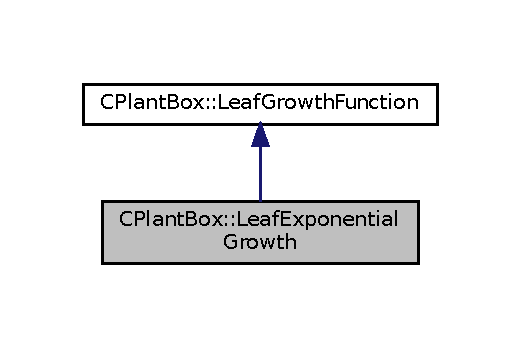
\includegraphics[width=250pt]{classCPlantBox_1_1LeafExponentialGrowth__inherit__graph}
\end{center}
\end{figure}


Collaboration diagram for C\+Plant\+Box\+:\+:Leaf\+Exponential\+Growth\+:\nopagebreak
\begin{figure}[H]
\begin{center}
\leavevmode
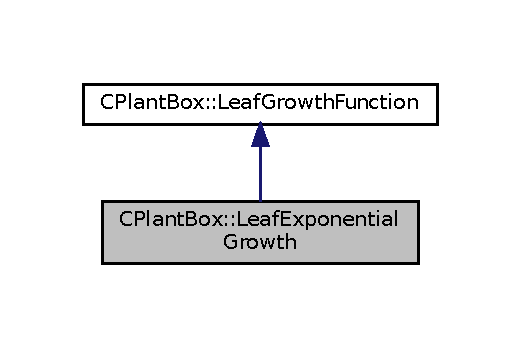
\includegraphics[width=250pt]{classCPlantBox_1_1LeafExponentialGrowth__coll__graph}
\end{center}
\end{figure}
\subsection*{Public Member Functions}
\begin{DoxyCompactItemize}
\item 
virtual double \hyperlink{classCPlantBox_1_1LeafExponentialGrowth_a734c28895db7e1c378d5431d712a53c9}{Leafget\+Length} (double t, double r, double k, \hyperlink{classCPlantBox_1_1Organ}{Organ} $\ast$leaf) const
\item 
virtual double \hyperlink{classCPlantBox_1_1LeafExponentialGrowth_a31eabefa43aee62945250d7a909a3cee}{Leafget\+Age} (double l, double r, double k, \hyperlink{classCPlantBox_1_1Organ}{Organ} $\ast$leaf) const
\end{DoxyCompactItemize}


\subsection{Detailed Description}
\hyperlink{classCPlantBox_1_1ExponentialGrowth}{Exponential\+Growth} elongates initially at constant rate r and slows down negative exponentially towards the maximum length k is reached 

\subsection{Member Function Documentation}
\mbox{\Hypertarget{classCPlantBox_1_1LeafExponentialGrowth_a31eabefa43aee62945250d7a909a3cee}\label{classCPlantBox_1_1LeafExponentialGrowth_a31eabefa43aee62945250d7a909a3cee}} 
\index{C\+Plant\+Box\+::\+Leaf\+Exponential\+Growth@{C\+Plant\+Box\+::\+Leaf\+Exponential\+Growth}!Leafget\+Age@{Leafget\+Age}}
\index{Leafget\+Age@{Leafget\+Age}!C\+Plant\+Box\+::\+Leaf\+Exponential\+Growth@{C\+Plant\+Box\+::\+Leaf\+Exponential\+Growth}}
\subsubsection{\texorpdfstring{Leafget\+Age()}{LeafgetAge()}}
{\footnotesize\ttfamily virtual double C\+Plant\+Box\+::\+Leaf\+Exponential\+Growth\+::\+Leafget\+Age (\begin{DoxyParamCaption}\item[{double}]{l,  }\item[{double}]{r,  }\item[{double}]{k,  }\item[{\hyperlink{classCPlantBox_1_1Organ}{Organ} $\ast$}]{leaf }\end{DoxyParamCaption}) const\hspace{0.3cm}{\ttfamily [inline]}, {\ttfamily [virtual]}}

\begin{DoxySeeAlso}{See also}
\hyperlink{classCPlantBox_1_1GrowthFunction}{Growth\+Function} 
\end{DoxySeeAlso}


Reimplemented from \hyperlink{classCPlantBox_1_1LeafGrowthFunction_a0893ec299fbd7566792e2ef9e2f58f2f}{C\+Plant\+Box\+::\+Leaf\+Growth\+Function}.

\mbox{\Hypertarget{classCPlantBox_1_1LeafExponentialGrowth_a734c28895db7e1c378d5431d712a53c9}\label{classCPlantBox_1_1LeafExponentialGrowth_a734c28895db7e1c378d5431d712a53c9}} 
\index{C\+Plant\+Box\+::\+Leaf\+Exponential\+Growth@{C\+Plant\+Box\+::\+Leaf\+Exponential\+Growth}!Leafget\+Length@{Leafget\+Length}}
\index{Leafget\+Length@{Leafget\+Length}!C\+Plant\+Box\+::\+Leaf\+Exponential\+Growth@{C\+Plant\+Box\+::\+Leaf\+Exponential\+Growth}}
\subsubsection{\texorpdfstring{Leafget\+Length()}{LeafgetLength()}}
{\footnotesize\ttfamily virtual double C\+Plant\+Box\+::\+Leaf\+Exponential\+Growth\+::\+Leafget\+Length (\begin{DoxyParamCaption}\item[{double}]{t,  }\item[{double}]{r,  }\item[{double}]{k,  }\item[{\hyperlink{classCPlantBox_1_1Organ}{Organ} $\ast$}]{leaf }\end{DoxyParamCaption}) const\hspace{0.3cm}{\ttfamily [inline]}, {\ttfamily [virtual]}}

\begin{DoxySeeAlso}{See also}
\hyperlink{classCPlantBox_1_1GrowthFunction}{Growth\+Function} 
\end{DoxySeeAlso}


Reimplemented from \hyperlink{classCPlantBox_1_1LeafGrowthFunction_a6261339dd2731a2cf33dc1fa111c9eaa}{C\+Plant\+Box\+::\+Leaf\+Growth\+Function}.



The documentation for this class was generated from the following file\+:\begin{DoxyCompactItemize}
\item 
src/Leaf\+Growth.\+h\end{DoxyCompactItemize}

\hypertarget{classCPlantBox_1_1LeafGravitropism}{}\section{C\+Plant\+Box\+:\+:Leaf\+Gravitropism Class Reference}
\label{classCPlantBox_1_1LeafGravitropism}\index{C\+Plant\+Box\+::\+Leaf\+Gravitropism@{C\+Plant\+Box\+::\+Leaf\+Gravitropism}}


{\ttfamily \#include $<$Leaf\+Tropism.\+h$>$}



Inheritance diagram for C\+Plant\+Box\+:\+:Leaf\+Gravitropism\+:\nopagebreak
\begin{figure}[H]
\begin{center}
\leavevmode
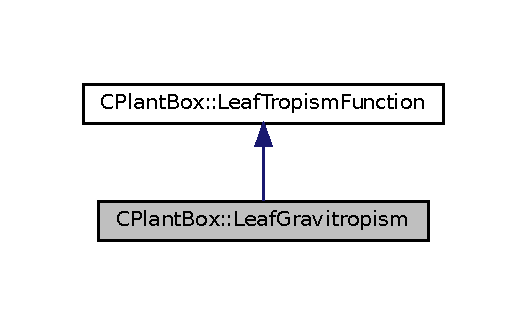
\includegraphics[width=253pt]{classCPlantBox_1_1LeafGravitropism__inherit__graph}
\end{center}
\end{figure}


Collaboration diagram for C\+Plant\+Box\+:\+:Leaf\+Gravitropism\+:\nopagebreak
\begin{figure}[H]
\begin{center}
\leavevmode
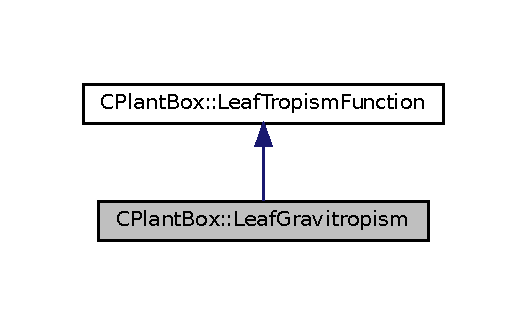
\includegraphics[width=253pt]{classCPlantBox_1_1LeafGravitropism__coll__graph}
\end{center}
\end{figure}
\subsection*{Public Member Functions}
\begin{DoxyCompactItemize}
\item 
\hyperlink{classCPlantBox_1_1LeafGravitropism_a23f0150896076ab7a358414c9aa1d5b4}{Leaf\+Gravitropism} (double \hyperlink{classCPlantBox_1_1LeafTropismFunction_a21d8d756f8b9f6015b546def33b01c89}{n}, double \hyperlink{classCPlantBox_1_1LeafTropismFunction_a82a3dc11056a65501bc4535749c304b6}{sigma})
\item 
virtual double \hyperlink{classCPlantBox_1_1LeafGravitropism_ab0836658683f5364fef25bafc7ac610e}{leaftropism\+Objective} (const \hyperlink{classCPlantBox_1_1Vector3d}{Vector3d} \&pos, \hyperlink{classCPlantBox_1_1Matrix3d}{Matrix3d} old, double a, double b, double dx, const \hyperlink{classCPlantBox_1_1Organ}{Organ} $\ast$leaf) override
\begin{DoxyCompactList}\small\item\em \hyperlink{classCPlantBox_1_1TropismFunction_adb52b88734a94fe1365a00e02c7e6be5}{Tropism\+Function\+::get\+Heading} minimizes this function,. \end{DoxyCompactList}\end{DoxyCompactItemize}
\subsection*{Additional Inherited Members}


\subsection{Detailed Description}
\hyperlink{classCPlantBox_1_1Gravitropism}{Gravitropism}\+: the tendency to grow downwards 

\subsection{Constructor \& Destructor Documentation}
\mbox{\Hypertarget{classCPlantBox_1_1LeafGravitropism_a23f0150896076ab7a358414c9aa1d5b4}\label{classCPlantBox_1_1LeafGravitropism_a23f0150896076ab7a358414c9aa1d5b4}} 
\index{C\+Plant\+Box\+::\+Leaf\+Gravitropism@{C\+Plant\+Box\+::\+Leaf\+Gravitropism}!Leaf\+Gravitropism@{Leaf\+Gravitropism}}
\index{Leaf\+Gravitropism@{Leaf\+Gravitropism}!C\+Plant\+Box\+::\+Leaf\+Gravitropism@{C\+Plant\+Box\+::\+Leaf\+Gravitropism}}
\subsubsection{\texorpdfstring{Leaf\+Gravitropism()}{LeafGravitropism()}}
{\footnotesize\ttfamily C\+Plant\+Box\+::\+Leaf\+Gravitropism\+::\+Leaf\+Gravitropism (\begin{DoxyParamCaption}\item[{double}]{n,  }\item[{double}]{sigma }\end{DoxyParamCaption})\hspace{0.3cm}{\ttfamily [inline]}}

\begin{DoxySeeAlso}{See also}
\hyperlink{classCPlantBox_1_1TropismFunction}{Tropism\+Function} 
\end{DoxySeeAlso}


\subsection{Member Function Documentation}
\mbox{\Hypertarget{classCPlantBox_1_1LeafGravitropism_ab0836658683f5364fef25bafc7ac610e}\label{classCPlantBox_1_1LeafGravitropism_ab0836658683f5364fef25bafc7ac610e}} 
\index{C\+Plant\+Box\+::\+Leaf\+Gravitropism@{C\+Plant\+Box\+::\+Leaf\+Gravitropism}!leaftropism\+Objective@{leaftropism\+Objective}}
\index{leaftropism\+Objective@{leaftropism\+Objective}!C\+Plant\+Box\+::\+Leaf\+Gravitropism@{C\+Plant\+Box\+::\+Leaf\+Gravitropism}}
\subsubsection{\texorpdfstring{leaftropism\+Objective()}{leaftropismObjective()}}
{\footnotesize\ttfamily virtual double C\+Plant\+Box\+::\+Leaf\+Gravitropism\+::leaftropism\+Objective (\begin{DoxyParamCaption}\item[{const \hyperlink{classCPlantBox_1_1Vector3d}{Vector3d} \&}]{pos,  }\item[{\hyperlink{classCPlantBox_1_1Matrix3d}{Matrix3d}}]{old,  }\item[{double}]{a,  }\item[{double}]{b,  }\item[{double}]{dx,  }\item[{const \hyperlink{classCPlantBox_1_1Organ}{Organ} $\ast$}]{leaf }\end{DoxyParamCaption})\hspace{0.3cm}{\ttfamily [inline]}, {\ttfamily [override]}, {\ttfamily [virtual]}}



\hyperlink{classCPlantBox_1_1TropismFunction_adb52b88734a94fe1365a00e02c7e6be5}{Tropism\+Function\+::get\+Heading} minimizes this function,. 

\begin{DoxySeeAlso}{See also}
\hyperlink{classCPlantBox_1_1TropismFunction_adb52b88734a94fe1365a00e02c7e6be5}{Tropism\+Function\+::get\+Heading} and 

\hyperlink{classCPlantBox_1_1TropismFunction_a4f2c79fff55d1398c98a070dd8ebbe08}{Tropism\+Function\+::tropism\+Objective} 
\end{DoxySeeAlso}


Reimplemented from \hyperlink{classCPlantBox_1_1LeafTropismFunction_ab89f5f7e80103d80681bc8cadc220dba}{C\+Plant\+Box\+::\+Leaf\+Tropism\+Function}.



The documentation for this class was generated from the following file\+:\begin{DoxyCompactItemize}
\item 
src/Leaf\+Tropism.\+h\end{DoxyCompactItemize}

\hypertarget{classCPlantBox_1_1LeafGrowthFunction}{}\section{C\+Plant\+Box\+:\+:Leaf\+Growth\+Function Class Reference}
\label{classCPlantBox_1_1LeafGrowthFunction}\index{C\+Plant\+Box\+::\+Leaf\+Growth\+Function@{C\+Plant\+Box\+::\+Leaf\+Growth\+Function}}


{\ttfamily \#include $<$Leaf\+Growth.\+h$>$}



Inheritance diagram for C\+Plant\+Box\+:\+:Leaf\+Growth\+Function\+:\nopagebreak
\begin{figure}[H]
\begin{center}
\leavevmode
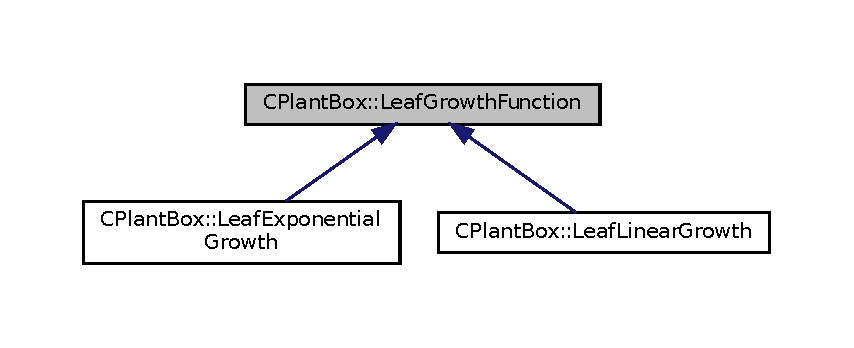
\includegraphics[width=350pt]{classCPlantBox_1_1LeafGrowthFunction__inherit__graph}
\end{center}
\end{figure}
\subsection*{Public Member Functions}
\begin{DoxyCompactItemize}
\item 
virtual double \hyperlink{classCPlantBox_1_1LeafGrowthFunction_a6261339dd2731a2cf33dc1fa111c9eaa}{Leafget\+Length} (double t, double r, double k, \hyperlink{classCPlantBox_1_1Organ}{Organ} $\ast$leaf) const
\begin{DoxyCompactList}\small\item\em Returns root length at root age t. \end{DoxyCompactList}\item 
virtual double \hyperlink{classCPlantBox_1_1LeafGrowthFunction_a0893ec299fbd7566792e2ef9e2f58f2f}{Leafget\+Age} (double l, double r, double k, \hyperlink{classCPlantBox_1_1Organ}{Organ} $\ast$leaf) const
\begin{DoxyCompactList}\small\item\em Returns the age of a root of length l. \end{DoxyCompactList}\end{DoxyCompactItemize}


\subsection{Detailed Description}
Abstract base class to all growth functions\+: currently \hyperlink{classCPlantBox_1_1LinearGrowth}{Linear\+Growth} and \hyperlink{classCPlantBox_1_1ExponentialGrowth}{Exponential\+Growth}

If new classes are created, they have to be added to the vector gf in in Root\+System. 

\subsection{Member Function Documentation}
\mbox{\Hypertarget{classCPlantBox_1_1LeafGrowthFunction_a0893ec299fbd7566792e2ef9e2f58f2f}\label{classCPlantBox_1_1LeafGrowthFunction_a0893ec299fbd7566792e2ef9e2f58f2f}} 
\index{C\+Plant\+Box\+::\+Leaf\+Growth\+Function@{C\+Plant\+Box\+::\+Leaf\+Growth\+Function}!Leafget\+Age@{Leafget\+Age}}
\index{Leafget\+Age@{Leafget\+Age}!C\+Plant\+Box\+::\+Leaf\+Growth\+Function@{C\+Plant\+Box\+::\+Leaf\+Growth\+Function}}
\subsubsection{\texorpdfstring{Leafget\+Age()}{LeafgetAge()}}
{\footnotesize\ttfamily virtual double C\+Plant\+Box\+::\+Leaf\+Growth\+Function\+::\+Leafget\+Age (\begin{DoxyParamCaption}\item[{double}]{l,  }\item[{double}]{r,  }\item[{double}]{k,  }\item[{\hyperlink{classCPlantBox_1_1Organ}{Organ} $\ast$}]{leaf }\end{DoxyParamCaption}) const\hspace{0.3cm}{\ttfamily [inline]}, {\ttfamily [virtual]}}



Returns the age of a root of length l. 

Returns the age of a root of length l


\begin{DoxyParams}{Parameters}
{\em l} & root length \mbox{[}cm\mbox{]} \\
\hline
{\em r} & initial growth rate \mbox{[}cm/day\mbox{]} \\
\hline
{\em k} & maximal root length \mbox{[}cm\mbox{]} \\
\hline
{\em root} & points to the root in case more information is needed\\
\hline
\end{DoxyParams}
\begin{DoxyReturn}{Returns}
root age \mbox{[}day\mbox{]} 
\end{DoxyReturn}


Reimplemented in \hyperlink{classCPlantBox_1_1LeafExponentialGrowth_a31eabefa43aee62945250d7a909a3cee}{C\+Plant\+Box\+::\+Leaf\+Exponential\+Growth}, and \hyperlink{classCPlantBox_1_1LeafLinearGrowth_ab66497e86721f7ba08d89ab3a78582d9}{C\+Plant\+Box\+::\+Leaf\+Linear\+Growth}.

\mbox{\Hypertarget{classCPlantBox_1_1LeafGrowthFunction_a6261339dd2731a2cf33dc1fa111c9eaa}\label{classCPlantBox_1_1LeafGrowthFunction_a6261339dd2731a2cf33dc1fa111c9eaa}} 
\index{C\+Plant\+Box\+::\+Leaf\+Growth\+Function@{C\+Plant\+Box\+::\+Leaf\+Growth\+Function}!Leafget\+Length@{Leafget\+Length}}
\index{Leafget\+Length@{Leafget\+Length}!C\+Plant\+Box\+::\+Leaf\+Growth\+Function@{C\+Plant\+Box\+::\+Leaf\+Growth\+Function}}
\subsubsection{\texorpdfstring{Leafget\+Length()}{LeafgetLength()}}
{\footnotesize\ttfamily virtual double C\+Plant\+Box\+::\+Leaf\+Growth\+Function\+::\+Leafget\+Length (\begin{DoxyParamCaption}\item[{double}]{t,  }\item[{double}]{r,  }\item[{double}]{k,  }\item[{\hyperlink{classCPlantBox_1_1Organ}{Organ} $\ast$}]{leaf }\end{DoxyParamCaption}) const\hspace{0.3cm}{\ttfamily [inline]}, {\ttfamily [virtual]}}



Returns root length at root age t. 

Returns root length at root age t


\begin{DoxyParams}{Parameters}
{\em t} & root age \mbox{[}day\mbox{]} \\
\hline
{\em r} & initial growth rate \mbox{[}cm/day\mbox{]} \\
\hline
{\em k} & maximal root length \mbox{[}cm\mbox{]} \\
\hline
{\em root} & points to the root in case more information is needed\\
\hline
\end{DoxyParams}
\begin{DoxyReturn}{Returns}
root length \mbox{[}cm\mbox{]} 
\end{DoxyReturn}


Reimplemented in \hyperlink{classCPlantBox_1_1LeafExponentialGrowth_a734c28895db7e1c378d5431d712a53c9}{C\+Plant\+Box\+::\+Leaf\+Exponential\+Growth}, and \hyperlink{classCPlantBox_1_1LeafLinearGrowth_a46f07fae546309d050777f1b5350ecf0}{C\+Plant\+Box\+::\+Leaf\+Linear\+Growth}.



The documentation for this class was generated from the following file\+:\begin{DoxyCompactItemize}
\item 
src/Leaf\+Growth.\+h\end{DoxyCompactItemize}

\hypertarget{classCPlantBox_1_1LeafLinearGrowth}{}\section{C\+Plant\+Box\+:\+:Leaf\+Linear\+Growth Class Reference}
\label{classCPlantBox_1_1LeafLinearGrowth}\index{C\+Plant\+Box\+::\+Leaf\+Linear\+Growth@{C\+Plant\+Box\+::\+Leaf\+Linear\+Growth}}


{\ttfamily \#include $<$Leaf\+Growth.\+h$>$}



Inheritance diagram for C\+Plant\+Box\+:\+:Leaf\+Linear\+Growth\+:\nopagebreak
\begin{figure}[H]
\begin{center}
\leavevmode
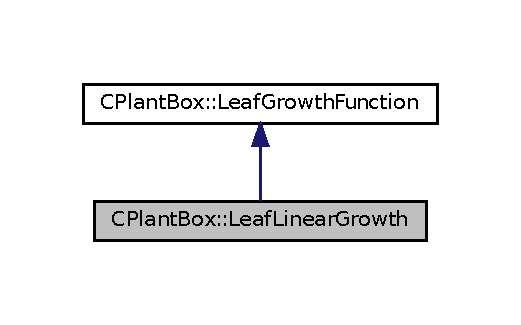
\includegraphics[width=250pt]{classCPlantBox_1_1LeafLinearGrowth__inherit__graph}
\end{center}
\end{figure}


Collaboration diagram for C\+Plant\+Box\+:\+:Leaf\+Linear\+Growth\+:\nopagebreak
\begin{figure}[H]
\begin{center}
\leavevmode
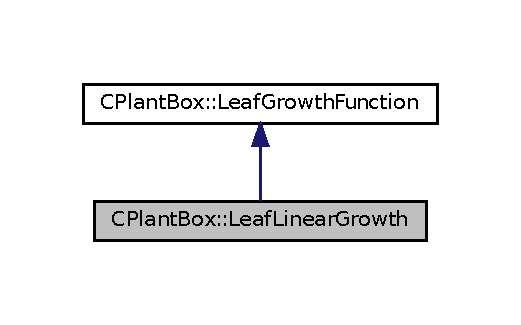
\includegraphics[width=250pt]{classCPlantBox_1_1LeafLinearGrowth__coll__graph}
\end{center}
\end{figure}
\subsection*{Public Member Functions}
\begin{DoxyCompactItemize}
\item 
virtual double \hyperlink{classCPlantBox_1_1LeafLinearGrowth_a46f07fae546309d050777f1b5350ecf0}{Leafget\+Length} (double t, double r, double k, \hyperlink{classCPlantBox_1_1Organ}{Organ} $\ast$leaf) const
\item 
virtual double \hyperlink{classCPlantBox_1_1LeafLinearGrowth_ab66497e86721f7ba08d89ab3a78582d9}{Leafget\+Age} (double l, double r, double k, \hyperlink{classCPlantBox_1_1Organ}{Organ} $\ast$leaf) const
\end{DoxyCompactItemize}


\subsection{Detailed Description}
\hyperlink{classCPlantBox_1_1LinearGrowth}{Linear\+Growth} elongates at constant rate until the maximal length k is reached 

\subsection{Member Function Documentation}
\mbox{\Hypertarget{classCPlantBox_1_1LeafLinearGrowth_ab66497e86721f7ba08d89ab3a78582d9}\label{classCPlantBox_1_1LeafLinearGrowth_ab66497e86721f7ba08d89ab3a78582d9}} 
\index{C\+Plant\+Box\+::\+Leaf\+Linear\+Growth@{C\+Plant\+Box\+::\+Leaf\+Linear\+Growth}!Leafget\+Age@{Leafget\+Age}}
\index{Leafget\+Age@{Leafget\+Age}!C\+Plant\+Box\+::\+Leaf\+Linear\+Growth@{C\+Plant\+Box\+::\+Leaf\+Linear\+Growth}}
\subsubsection{\texorpdfstring{Leafget\+Age()}{LeafgetAge()}}
{\footnotesize\ttfamily virtual double C\+Plant\+Box\+::\+Leaf\+Linear\+Growth\+::\+Leafget\+Age (\begin{DoxyParamCaption}\item[{double}]{l,  }\item[{double}]{r,  }\item[{double}]{k,  }\item[{\hyperlink{classCPlantBox_1_1Organ}{Organ} $\ast$}]{leaf }\end{DoxyParamCaption}) const\hspace{0.3cm}{\ttfamily [inline]}, {\ttfamily [virtual]}}

\begin{DoxySeeAlso}{See also}
\hyperlink{classCPlantBox_1_1GrowthFunction}{Growth\+Function} 
\end{DoxySeeAlso}


Reimplemented from \hyperlink{classCPlantBox_1_1LeafGrowthFunction_a0893ec299fbd7566792e2ef9e2f58f2f}{C\+Plant\+Box\+::\+Leaf\+Growth\+Function}.

\mbox{\Hypertarget{classCPlantBox_1_1LeafLinearGrowth_a46f07fae546309d050777f1b5350ecf0}\label{classCPlantBox_1_1LeafLinearGrowth_a46f07fae546309d050777f1b5350ecf0}} 
\index{C\+Plant\+Box\+::\+Leaf\+Linear\+Growth@{C\+Plant\+Box\+::\+Leaf\+Linear\+Growth}!Leafget\+Length@{Leafget\+Length}}
\index{Leafget\+Length@{Leafget\+Length}!C\+Plant\+Box\+::\+Leaf\+Linear\+Growth@{C\+Plant\+Box\+::\+Leaf\+Linear\+Growth}}
\subsubsection{\texorpdfstring{Leafget\+Length()}{LeafgetLength()}}
{\footnotesize\ttfamily virtual double C\+Plant\+Box\+::\+Leaf\+Linear\+Growth\+::\+Leafget\+Length (\begin{DoxyParamCaption}\item[{double}]{t,  }\item[{double}]{r,  }\item[{double}]{k,  }\item[{\hyperlink{classCPlantBox_1_1Organ}{Organ} $\ast$}]{leaf }\end{DoxyParamCaption}) const\hspace{0.3cm}{\ttfamily [inline]}, {\ttfamily [virtual]}}

\begin{DoxySeeAlso}{See also}
\hyperlink{classCPlantBox_1_1GrowthFunction}{Growth\+Function} 
\end{DoxySeeAlso}


Reimplemented from \hyperlink{classCPlantBox_1_1LeafGrowthFunction_a6261339dd2731a2cf33dc1fa111c9eaa}{C\+Plant\+Box\+::\+Leaf\+Growth\+Function}.



The documentation for this class was generated from the following file\+:\begin{DoxyCompactItemize}
\item 
src/Leaf\+Growth.\+h\end{DoxyCompactItemize}

\hypertarget{classCPlantBox_1_1LeafParameter}{}\section{C\+Plant\+Box\+:\+:Leaf\+Parameter Class Reference}
\label{classCPlantBox_1_1LeafParameter}\index{C\+Plant\+Box\+::\+Leaf\+Parameter@{C\+Plant\+Box\+::\+Leaf\+Parameter}}


{\ttfamily \#include $<$Model\+Parameter.\+h$>$}



Inheritance diagram for C\+Plant\+Box\+:\+:Leaf\+Parameter\+:\nopagebreak
\begin{figure}[H]
\begin{center}
\leavevmode
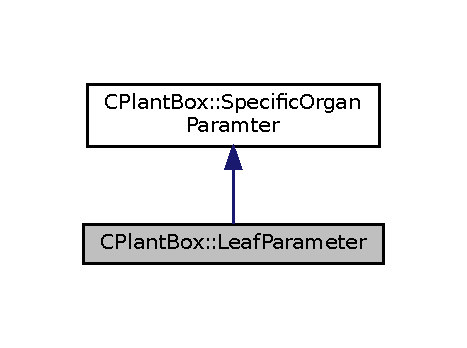
\includegraphics[width=224pt]{classCPlantBox_1_1LeafParameter__inherit__graph}
\end{center}
\end{figure}


Collaboration diagram for C\+Plant\+Box\+:\+:Leaf\+Parameter\+:\nopagebreak
\begin{figure}[H]
\begin{center}
\leavevmode
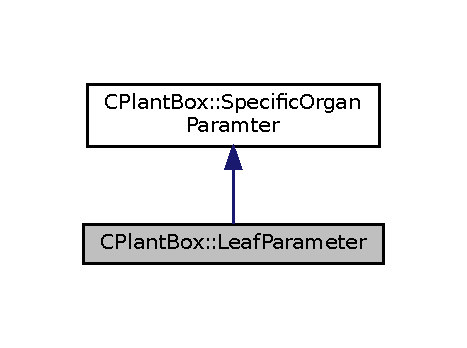
\includegraphics[width=224pt]{classCPlantBox_1_1LeafParameter__coll__graph}
\end{center}
\end{figure}
\subsection*{Public Member Functions}
\begin{DoxyCompactItemize}
\item 
\mbox{\Hypertarget{classCPlantBox_1_1LeafParameter_afcf5e061df816b74198539e2dd22ec8f}\label{classCPlantBox_1_1LeafParameter_afcf5e061df816b74198539e2dd22ec8f}} 
\hyperlink{classCPlantBox_1_1LeafParameter_afcf5e061df816b74198539e2dd22ec8f}{Leaf\+Parameter} (int type, double \hyperlink{classCPlantBox_1_1LeafParameter_a9e7f83b4d00f065f57828a0095760d99}{lb}, double \hyperlink{classCPlantBox_1_1LeafParameter_ac47a1d37fbe865651caadea39a6f7e2c}{la}, const std\+::vector$<$ double $>$ \&\hyperlink{classCPlantBox_1_1LeafParameter_aeafebf5e63919a27d47f31dc09afddc8}{ln}, double \hyperlink{classCPlantBox_1_1LeafParameter_ab3a0d010eb7f48c4c65bcb4ff89f90e9}{r}, double \hyperlink{classCPlantBox_1_1LeafParameter_a7054dac50e123c9b8f131dc44b986e07}{a}, double \hyperlink{classCPlantBox_1_1LeafParameter_a05e81f99fb9363caca8b382b0dc021ca}{theta}, double \hyperlink{classCPlantBox_1_1LeafParameter_afece895e2e0669022f3813e9bd4263c6}{rlt}, int lnf)
\begin{DoxyCompactList}\small\item\em Constructor setting all parameters. \end{DoxyCompactList}\item 
double \hyperlink{classCPlantBox_1_1LeafParameter_a5a14e0f70c9e00cdcafd4fb86b6ef0ca}{getK} () const
\begin{DoxyCompactList}\small\item\em Returns the exact maximal root length of this realization \mbox{[}cm\mbox{]}. \end{DoxyCompactList}\item 
\mbox{\Hypertarget{classCPlantBox_1_1LeafParameter_aff7069a9fef9bd5a2edabd59b237c2d4}\label{classCPlantBox_1_1LeafParameter_aff7069a9fef9bd5a2edabd59b237c2d4}} 
void \hyperlink{classCPlantBox_1_1LeafParameter_aff7069a9fef9bd5a2edabd59b237c2d4}{write} (std\+::ostream \&cout) const
\begin{DoxyCompactList}\small\item\em Writes parameters for debugging. \end{DoxyCompactList}\item 
\mbox{\Hypertarget{classCPlantBox_1_1LeafParameter_ac6f780e3619f958dde05dc1871ce4faa}\label{classCPlantBox_1_1LeafParameter_ac6f780e3619f958dde05dc1871ce4faa}} 
std\+::string \hyperlink{classCPlantBox_1_1LeafParameter_ac6f780e3619f958dde05dc1871ce4faa}{to\+String} () const
\begin{DoxyCompactList}\small\item\em String representation using \hyperlink{classCPlantBox_1_1RootParameter_aed958341f67d2bb36e1480e531732535}{Root\+Parameter\+::write}. \end{DoxyCompactList}\end{DoxyCompactItemize}
\subsection*{Public Attributes}
\begin{DoxyCompactItemize}
\item 
\mbox{\Hypertarget{classCPlantBox_1_1LeafParameter_a9e7f83b4d00f065f57828a0095760d99}\label{classCPlantBox_1_1LeafParameter_a9e7f83b4d00f065f57828a0095760d99}} 
double \hyperlink{classCPlantBox_1_1LeafParameter_a9e7f83b4d00f065f57828a0095760d99}{lb} = 0.
\begin{DoxyCompactList}\small\item\em Basal zone \mbox{[}cm\mbox{]}. \end{DoxyCompactList}\item 
\mbox{\Hypertarget{classCPlantBox_1_1LeafParameter_ac47a1d37fbe865651caadea39a6f7e2c}\label{classCPlantBox_1_1LeafParameter_ac47a1d37fbe865651caadea39a6f7e2c}} 
double \hyperlink{classCPlantBox_1_1LeafParameter_ac47a1d37fbe865651caadea39a6f7e2c}{la} = 0.
\begin{DoxyCompactList}\small\item\em Apical zone \mbox{[}cm\mbox{]};. \end{DoxyCompactList}\item 
\mbox{\Hypertarget{classCPlantBox_1_1LeafParameter_ab3a0d010eb7f48c4c65bcb4ff89f90e9}\label{classCPlantBox_1_1LeafParameter_ab3a0d010eb7f48c4c65bcb4ff89f90e9}} 
double \hyperlink{classCPlantBox_1_1LeafParameter_ab3a0d010eb7f48c4c65bcb4ff89f90e9}{r} = 0.
\begin{DoxyCompactList}\small\item\em Initial growth rate \mbox{[}cm day-\/1\mbox{]}. \end{DoxyCompactList}\item 
\mbox{\Hypertarget{classCPlantBox_1_1LeafParameter_a7054dac50e123c9b8f131dc44b986e07}\label{classCPlantBox_1_1LeafParameter_a7054dac50e123c9b8f131dc44b986e07}} 
double \hyperlink{classCPlantBox_1_1LeafParameter_a7054dac50e123c9b8f131dc44b986e07}{a} = 0.
\begin{DoxyCompactList}\small\item\em \hyperlink{classCPlantBox_1_1Root}{Root} radius \mbox{[}cm\mbox{]}. \end{DoxyCompactList}\item 
\mbox{\Hypertarget{classCPlantBox_1_1LeafParameter_a05e81f99fb9363caca8b382b0dc021ca}\label{classCPlantBox_1_1LeafParameter_a05e81f99fb9363caca8b382b0dc021ca}} 
double \hyperlink{classCPlantBox_1_1LeafParameter_a05e81f99fb9363caca8b382b0dc021ca}{theta} = 0.
\begin{DoxyCompactList}\small\item\em Angle between root and parent root \mbox{[}rad\mbox{]}. \end{DoxyCompactList}\item 
\mbox{\Hypertarget{classCPlantBox_1_1LeafParameter_afece895e2e0669022f3813e9bd4263c6}\label{classCPlantBox_1_1LeafParameter_afece895e2e0669022f3813e9bd4263c6}} 
double \hyperlink{classCPlantBox_1_1LeafParameter_afece895e2e0669022f3813e9bd4263c6}{rlt} = 0.
\begin{DoxyCompactList}\small\item\em \hyperlink{classCPlantBox_1_1Root}{Root} life time \mbox{[}day\mbox{]}. \end{DoxyCompactList}\item 
\mbox{\Hypertarget{classCPlantBox_1_1LeafParameter_aeafebf5e63919a27d47f31dc09afddc8}\label{classCPlantBox_1_1LeafParameter_aeafebf5e63919a27d47f31dc09afddc8}} 
std\+::vector$<$ double $>$ \hyperlink{classCPlantBox_1_1LeafParameter_aeafebf5e63919a27d47f31dc09afddc8}{ln} = std\+::vector$<$double$>$()
\begin{DoxyCompactList}\small\item\em Inter-\/lateral distances \mbox{[}cm\mbox{]}. \end{DoxyCompactList}\item 
\mbox{\Hypertarget{classCPlantBox_1_1LeafParameter_a50ade6d628cf02832df79f1c856988a2}\label{classCPlantBox_1_1LeafParameter_a50ade6d628cf02832df79f1c856988a2}} 
int {\bfseries lnf} = 0
\end{DoxyCompactItemize}


\subsection{Detailed Description}
Parameter base class for specific organs Parameters of a single root (created by \hyperlink{classCPlantBox_1_1RootParameter}{Root\+Parameter}\+:realize) 

\subsection{Member Function Documentation}
\mbox{\Hypertarget{classCPlantBox_1_1LeafParameter_a5a14e0f70c9e00cdcafd4fb86b6ef0ca}\label{classCPlantBox_1_1LeafParameter_a5a14e0f70c9e00cdcafd4fb86b6ef0ca}} 
\index{C\+Plant\+Box\+::\+Leaf\+Parameter@{C\+Plant\+Box\+::\+Leaf\+Parameter}!getK@{getK}}
\index{getK@{getK}!C\+Plant\+Box\+::\+Leaf\+Parameter@{C\+Plant\+Box\+::\+Leaf\+Parameter}}
\subsubsection{\texorpdfstring{get\+K()}{getK()}}
{\footnotesize\ttfamily double C\+Plant\+Box\+::\+Leaf\+Parameter\+::getK (\begin{DoxyParamCaption}{ }\end{DoxyParamCaption}) const}



Returns the exact maximal root length of this realization \mbox{[}cm\mbox{]}. 

$\ast$$\ast$$\ast$$\ast$$\ast$$\ast$$\ast$$\ast$$\ast$$\ast$$\ast$$\ast$$\ast$$\ast$$\ast$$\ast$$\ast$$\ast$$\ast$$\ast$$\ast$$\ast$$\ast$$\ast$$\ast$$\ast$$\ast$$\ast$$\ast$$\ast$$\ast$$\ast$$\ast$$\ast$$\ast$$\ast$$\ast$$\ast$$\ast$$\ast$$\ast$$\ast$$\ast$$\ast$$\ast$$\ast$$\ast$$\ast$$\ast$$\ast$$\ast$$\ast$$\ast$$\ast$$\ast$$\ast$$\ast$$\ast$\+Another C\+O\+PY P\+A\+S\+TE to create leaf$\ast$$\ast$$\ast$$\ast$$\ast$$\ast$$\ast$$\ast$$\ast$$\ast$$\ast$$\ast$$\ast$$\ast$$\ast$$\ast$$\ast$$\ast$$\ast$$\ast$$\ast$$\ast$$\ast$$\ast$$\ast$$\ast$$\ast$$\ast$$\ast$$\ast$$\ast$$\ast$$\ast$$\ast$$\ast$$\ast$$\ast$$\ast$$\ast$$\ast$$\ast$$\ast$$\ast$$\ast$$\ast$$\ast$$\ast$$\ast$$\ast$$\ast$$\ast$$\ast$$\ast$$\ast$$\ast$$\ast$$\ast$$\ast$$\ast$$\ast$$\ast$$\ast$$\ast$$\ast$$\ast$$\ast$$\ast$$\ast$$\ast$$\ast$$\ast$$\ast$$\ast$$\ast$$\ast$$\ast$$\ast$$\ast$$\ast$$\ast$$\ast$$\ast$$\ast$$\ast$$\ast$$\ast$$\ast$$\ast$$\ast$$\ast$ 

The documentation for this class was generated from the following files\+:\begin{DoxyCompactItemize}
\item 
src/Model\+Parameter.\+h\item 
src/Model\+Parameter.\+cpp\end{DoxyCompactItemize}

\hypertarget{classCPlantBox_1_1LeafPhototropism}{}\section{C\+Plant\+Box\+:\+:Leaf\+Phototropism Class Reference}
\label{classCPlantBox_1_1LeafPhototropism}\index{C\+Plant\+Box\+::\+Leaf\+Phototropism@{C\+Plant\+Box\+::\+Leaf\+Phototropism}}


{\ttfamily \#include $<$Leaf\+Tropism.\+h$>$}



Inheritance diagram for C\+Plant\+Box\+:\+:Leaf\+Phototropism\+:\nopagebreak
\begin{figure}[H]
\begin{center}
\leavevmode
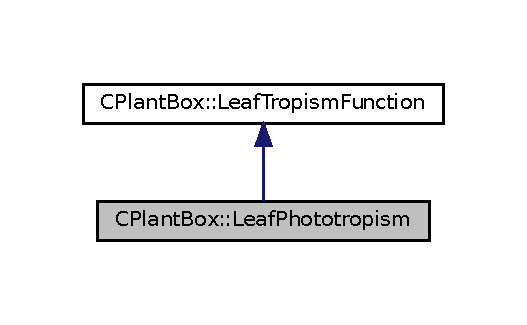
\includegraphics[width=253pt]{classCPlantBox_1_1LeafPhototropism__inherit__graph}
\end{center}
\end{figure}


Collaboration diagram for C\+Plant\+Box\+:\+:Leaf\+Phototropism\+:\nopagebreak
\begin{figure}[H]
\begin{center}
\leavevmode
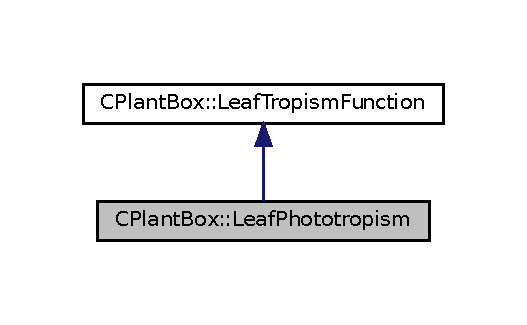
\includegraphics[width=253pt]{classCPlantBox_1_1LeafPhototropism__coll__graph}
\end{center}
\end{figure}
\subsection*{Public Member Functions}
\begin{DoxyCompactItemize}
\item 
\hyperlink{classCPlantBox_1_1LeafPhototropism_ad92daedd811b83ab7b6e8901dd9970dc}{Leaf\+Phototropism} (double \hyperlink{classCPlantBox_1_1LeafTropismFunction_a21d8d756f8b9f6015b546def33b01c89}{n}, double \hyperlink{classCPlantBox_1_1LeafTropismFunction_a82a3dc11056a65501bc4535749c304b6}{sigma}, \hyperlink{classCPlantBox_1_1SoilLookUp}{Soil\+Look\+Up} $\ast$soil)
\item 
virtual double \hyperlink{classCPlantBox_1_1LeafPhototropism_a9b9cee624adc576c2cc44b1b27b2ef0c}{leaftropism\+Objective} (const \hyperlink{classCPlantBox_1_1Vector3d}{Vector3d} \&pos, \hyperlink{classCPlantBox_1_1Matrix3d}{Matrix3d} old, double a, double b, double dx, const \hyperlink{classCPlantBox_1_1Organ}{Organ} $\ast$leaf) override
\begin{DoxyCompactList}\small\item\em \hyperlink{classCPlantBox_1_1LeafTropismFunction_a1440868221a834474e34e3a503a74572}{get\+Heading()} minimizes this function, \end{DoxyCompactList}\end{DoxyCompactItemize}
\subsection*{Additional Inherited Members}


\subsection{Detailed Description}
\hyperlink{classCPlantBox_1_1Hydrotropism}{Hydrotropism} (or Chemotropism, ...)\+: the tendency to grow towards a higher saturation (or concentration, ...) 

\subsection{Constructor \& Destructor Documentation}
\mbox{\Hypertarget{classCPlantBox_1_1LeafPhototropism_ad92daedd811b83ab7b6e8901dd9970dc}\label{classCPlantBox_1_1LeafPhototropism_ad92daedd811b83ab7b6e8901dd9970dc}} 
\index{C\+Plant\+Box\+::\+Leaf\+Phototropism@{C\+Plant\+Box\+::\+Leaf\+Phototropism}!Leaf\+Phototropism@{Leaf\+Phototropism}}
\index{Leaf\+Phototropism@{Leaf\+Phototropism}!C\+Plant\+Box\+::\+Leaf\+Phototropism@{C\+Plant\+Box\+::\+Leaf\+Phototropism}}
\subsubsection{\texorpdfstring{Leaf\+Phototropism()}{LeafPhototropism()}}
{\footnotesize\ttfamily C\+Plant\+Box\+::\+Leaf\+Phototropism\+::\+Leaf\+Phototropism (\begin{DoxyParamCaption}\item[{double}]{n,  }\item[{double}]{sigma,  }\item[{\hyperlink{classCPlantBox_1_1SoilLookUp}{Soil\+Look\+Up} $\ast$}]{soil }\end{DoxyParamCaption})\hspace{0.3cm}{\ttfamily [inline]}}

\begin{DoxySeeAlso}{See also}
\hyperlink{classCPlantBox_1_1TropismFunction}{Tropism\+Function} 
\end{DoxySeeAlso}


\subsection{Member Function Documentation}
\mbox{\Hypertarget{classCPlantBox_1_1LeafPhototropism_a9b9cee624adc576c2cc44b1b27b2ef0c}\label{classCPlantBox_1_1LeafPhototropism_a9b9cee624adc576c2cc44b1b27b2ef0c}} 
\index{C\+Plant\+Box\+::\+Leaf\+Phototropism@{C\+Plant\+Box\+::\+Leaf\+Phototropism}!leaftropism\+Objective@{leaftropism\+Objective}}
\index{leaftropism\+Objective@{leaftropism\+Objective}!C\+Plant\+Box\+::\+Leaf\+Phototropism@{C\+Plant\+Box\+::\+Leaf\+Phototropism}}
\subsubsection{\texorpdfstring{leaftropism\+Objective()}{leaftropismObjective()}}
{\footnotesize\ttfamily double C\+Plant\+Box\+::\+Leaf\+Phototropism\+::leaftropism\+Objective (\begin{DoxyParamCaption}\item[{const \hyperlink{classCPlantBox_1_1Vector3d}{Vector3d} \&}]{pos,  }\item[{\hyperlink{classCPlantBox_1_1Matrix3d}{Matrix3d}}]{old,  }\item[{double}]{a,  }\item[{double}]{b,  }\item[{double}]{dx,  }\item[{const \hyperlink{classCPlantBox_1_1Organ}{Organ} $\ast$}]{leaf }\end{DoxyParamCaption})\hspace{0.3cm}{\ttfamily [override]}, {\ttfamily [virtual]}}



\hyperlink{classCPlantBox_1_1LeafTropismFunction_a1440868221a834474e34e3a503a74572}{get\+Heading()} minimizes this function, 

\begin{DoxySeeAlso}{See also}
\hyperlink{classCPlantBox_1_1TropismFunction}{Tropism\+Function}
\end{DoxySeeAlso}
\hyperlink{classCPlantBox_1_1LeafTropismFunction_a1440868221a834474e34e3a503a74572}{get\+Heading()} minimizes this function, \begin{DoxySeeAlso}{See also}
\hyperlink{classCPlantBox_1_1TropismFunction_a4f2c79fff55d1398c98a070dd8ebbe08}{Tropism\+Function\+::tropism\+Objective} 
\end{DoxySeeAlso}
$<$ (-\/1) because we want to maximize the soil property 

Reimplemented from \hyperlink{classCPlantBox_1_1LeafTropismFunction_ab89f5f7e80103d80681bc8cadc220dba}{C\+Plant\+Box\+::\+Leaf\+Tropism\+Function}.



The documentation for this class was generated from the following files\+:\begin{DoxyCompactItemize}
\item 
src/Leaf\+Tropism.\+h\item 
src/Leaf\+Tropism.\+cpp\end{DoxyCompactItemize}

\hypertarget{classCPlantBox_1_1LeafPlagiotropism}{}\section{C\+Plant\+Box\+:\+:Leaf\+Plagiotropism Class Reference}
\label{classCPlantBox_1_1LeafPlagiotropism}\index{C\+Plant\+Box\+::\+Leaf\+Plagiotropism@{C\+Plant\+Box\+::\+Leaf\+Plagiotropism}}


{\ttfamily \#include $<$Leaf\+Tropism.\+h$>$}



Inheritance diagram for C\+Plant\+Box\+:\+:Leaf\+Plagiotropism\+:\nopagebreak
\begin{figure}[H]
\begin{center}
\leavevmode
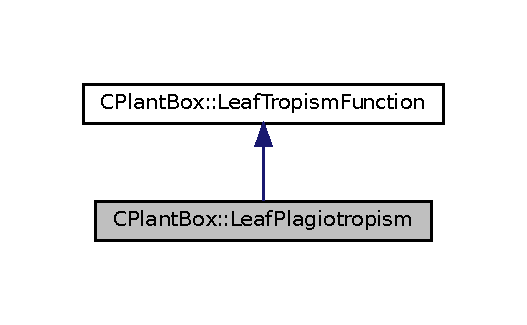
\includegraphics[width=253pt]{classCPlantBox_1_1LeafPlagiotropism__inherit__graph}
\end{center}
\end{figure}


Collaboration diagram for C\+Plant\+Box\+:\+:Leaf\+Plagiotropism\+:\nopagebreak
\begin{figure}[H]
\begin{center}
\leavevmode
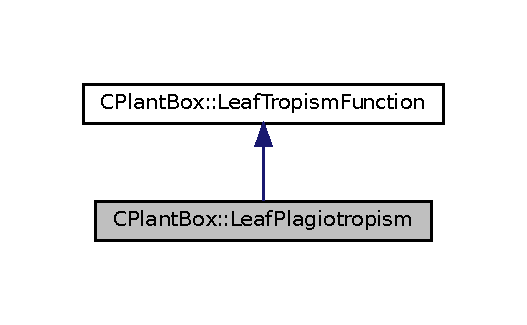
\includegraphics[width=253pt]{classCPlantBox_1_1LeafPlagiotropism__coll__graph}
\end{center}
\end{figure}
\subsection*{Public Member Functions}
\begin{DoxyCompactItemize}
\item 
\hyperlink{classCPlantBox_1_1LeafPlagiotropism_af130f22f6e7fae16e5d15b32ad5e0f69}{Leaf\+Plagiotropism} (double \hyperlink{classCPlantBox_1_1LeafTropismFunction_a21d8d756f8b9f6015b546def33b01c89}{n}, double \hyperlink{classCPlantBox_1_1LeafTropismFunction_a82a3dc11056a65501bc4535749c304b6}{sigma})
\item 
virtual double \hyperlink{classCPlantBox_1_1LeafPlagiotropism_af58514b24aae9a1020093d6955dadaaf}{leaftropism\+Objective} (const \hyperlink{classCPlantBox_1_1Vector3d}{Vector3d} \&pos, \hyperlink{classCPlantBox_1_1Matrix3d}{Matrix3d} old, double a, double b, double dx, const \hyperlink{classCPlantBox_1_1Organ}{Organ} $\ast$leaf) override
\begin{DoxyCompactList}\small\item\em \hyperlink{classCPlantBox_1_1LeafTropismFunction_a1440868221a834474e34e3a503a74572}{get\+Heading()} minimizes this function, \end{DoxyCompactList}\end{DoxyCompactItemize}
\subsection*{Additional Inherited Members}


\subsection{Detailed Description}
\hyperlink{classCPlantBox_1_1Plagiotropism}{Plagiotropism}\+: the tendency to stay in a horicontal layer 

\subsection{Constructor \& Destructor Documentation}
\mbox{\Hypertarget{classCPlantBox_1_1LeafPlagiotropism_af130f22f6e7fae16e5d15b32ad5e0f69}\label{classCPlantBox_1_1LeafPlagiotropism_af130f22f6e7fae16e5d15b32ad5e0f69}} 
\index{C\+Plant\+Box\+::\+Leaf\+Plagiotropism@{C\+Plant\+Box\+::\+Leaf\+Plagiotropism}!Leaf\+Plagiotropism@{Leaf\+Plagiotropism}}
\index{Leaf\+Plagiotropism@{Leaf\+Plagiotropism}!C\+Plant\+Box\+::\+Leaf\+Plagiotropism@{C\+Plant\+Box\+::\+Leaf\+Plagiotropism}}
\subsubsection{\texorpdfstring{Leaf\+Plagiotropism()}{LeafPlagiotropism()}}
{\footnotesize\ttfamily C\+Plant\+Box\+::\+Leaf\+Plagiotropism\+::\+Leaf\+Plagiotropism (\begin{DoxyParamCaption}\item[{double}]{n,  }\item[{double}]{sigma }\end{DoxyParamCaption})\hspace{0.3cm}{\ttfamily [inline]}}

\begin{DoxySeeAlso}{See also}
\hyperlink{classCPlantBox_1_1TropismFunction}{Tropism\+Function} 
\end{DoxySeeAlso}


\subsection{Member Function Documentation}
\mbox{\Hypertarget{classCPlantBox_1_1LeafPlagiotropism_af58514b24aae9a1020093d6955dadaaf}\label{classCPlantBox_1_1LeafPlagiotropism_af58514b24aae9a1020093d6955dadaaf}} 
\index{C\+Plant\+Box\+::\+Leaf\+Plagiotropism@{C\+Plant\+Box\+::\+Leaf\+Plagiotropism}!leaftropism\+Objective@{leaftropism\+Objective}}
\index{leaftropism\+Objective@{leaftropism\+Objective}!C\+Plant\+Box\+::\+Leaf\+Plagiotropism@{C\+Plant\+Box\+::\+Leaf\+Plagiotropism}}
\subsubsection{\texorpdfstring{leaftropism\+Objective()}{leaftropismObjective()}}
{\footnotesize\ttfamily virtual double C\+Plant\+Box\+::\+Leaf\+Plagiotropism\+::leaftropism\+Objective (\begin{DoxyParamCaption}\item[{const \hyperlink{classCPlantBox_1_1Vector3d}{Vector3d} \&}]{pos,  }\item[{\hyperlink{classCPlantBox_1_1Matrix3d}{Matrix3d}}]{old,  }\item[{double}]{a,  }\item[{double}]{b,  }\item[{double}]{dx,  }\item[{const \hyperlink{classCPlantBox_1_1Organ}{Organ} $\ast$}]{leaf }\end{DoxyParamCaption})\hspace{0.3cm}{\ttfamily [inline]}, {\ttfamily [override]}, {\ttfamily [virtual]}}



\hyperlink{classCPlantBox_1_1LeafTropismFunction_a1440868221a834474e34e3a503a74572}{get\+Heading()} minimizes this function, 

\begin{DoxySeeAlso}{See also}
\hyperlink{classCPlantBox_1_1TropismFunction}{Tropism\+Function} 
\end{DoxySeeAlso}


Reimplemented from \hyperlink{classCPlantBox_1_1LeafTropismFunction_ab89f5f7e80103d80681bc8cadc220dba}{C\+Plant\+Box\+::\+Leaf\+Tropism\+Function}.



The documentation for this class was generated from the following file\+:\begin{DoxyCompactItemize}
\item 
src/Leaf\+Tropism.\+h\end{DoxyCompactItemize}

\hypertarget{classCPlantBox_1_1LeafRandomOrganParameter}{}\section{C\+Plant\+Box\+:\+:Leaf\+Random\+Organ\+Parameter Class Reference}
\label{classCPlantBox_1_1LeafRandomOrganParameter}\index{C\+Plant\+Box\+::\+Leaf\+Random\+Organ\+Parameter@{C\+Plant\+Box\+::\+Leaf\+Random\+Organ\+Parameter}}


{\ttfamily \#include $<$Model\+Parameter.\+h$>$}



Inheritance diagram for C\+Plant\+Box\+:\+:Leaf\+Random\+Organ\+Parameter\+:\nopagebreak
\begin{figure}[H]
\begin{center}
\leavevmode
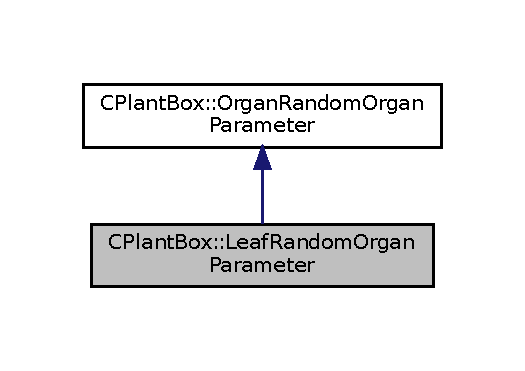
\includegraphics[width=252pt]{classCPlantBox_1_1LeafRandomOrganParameter__inherit__graph}
\end{center}
\end{figure}


Collaboration diagram for C\+Plant\+Box\+:\+:Leaf\+Random\+Organ\+Parameter\+:\nopagebreak
\begin{figure}[H]
\begin{center}
\leavevmode
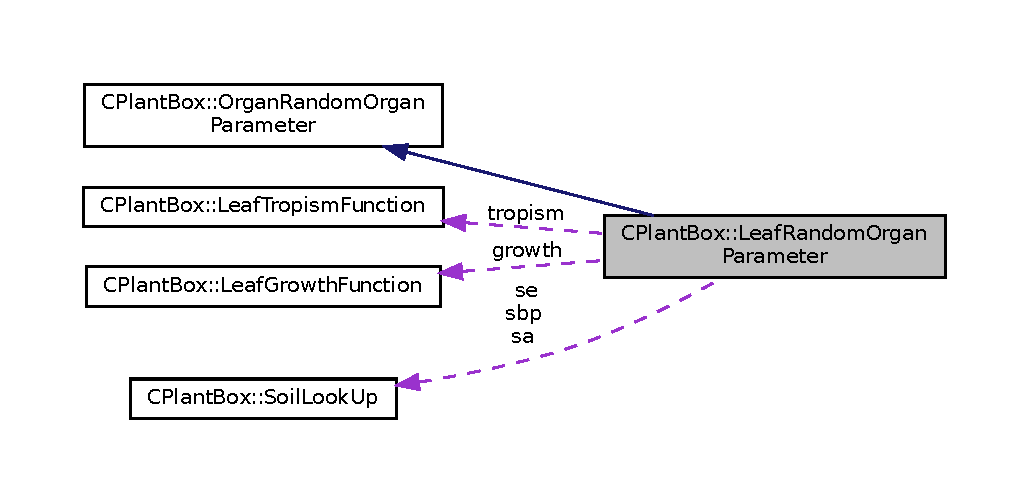
\includegraphics[width=350pt]{classCPlantBox_1_1LeafRandomOrganParameter__coll__graph}
\end{center}
\end{figure}
\subsection*{Public Types}
\begin{DoxyCompactItemize}
\item 
\mbox{\Hypertarget{classCPlantBox_1_1LeafRandomOrganParameter_adee79852a22b74f67005bdd1dde99351}\label{classCPlantBox_1_1LeafRandomOrganParameter_adee79852a22b74f67005bdd1dde99351}} 
enum {\bfseries Leaf\+Tropism\+Types} \{ \newline
{\bfseries tt\+\_\+plagio} = 0, 
{\bfseries tt\+\_\+gravi} = 1, 
{\bfseries tt\+\_\+exo} = 2, 
{\bfseries tt\+\_\+hydro} = 3, 
\newline
{\bfseries tt\+\_\+antigravi} = 4
 \}
\item 
\mbox{\Hypertarget{classCPlantBox_1_1LeafRandomOrganParameter_acc5540fca1aeae1c93cb435658d29eff}\label{classCPlantBox_1_1LeafRandomOrganParameter_acc5540fca1aeae1c93cb435658d29eff}} 
enum {\bfseries Leaf\+Growth\+Function\+Types} \{ {\bfseries gft\+\_\+negexp} = 1, 
{\bfseries gft\+\_\+linear} = 2
 \}
\end{DoxyCompactItemize}
\subsection*{Public Member Functions}
\begin{DoxyCompactItemize}
\item 
\mbox{\Hypertarget{classCPlantBox_1_1LeafRandomOrganParameter_af1827c611818d9bbd280f4052187edeb}\label{classCPlantBox_1_1LeafRandomOrganParameter_af1827c611818d9bbd280f4052187edeb}} 
\hyperlink{classCPlantBox_1_1LeafRandomOrganParameter_af1827c611818d9bbd280f4052187edeb}{Leaf\+Random\+Organ\+Parameter} ()
\begin{DoxyCompactList}\small\item\em default constructor \end{DoxyCompactList}\item 
void \hyperlink{classCPlantBox_1_1LeafRandomOrganParameter_acce175a540cc9cde00344a6336246a64}{set} (int type, double \hyperlink{classCPlantBox_1_1LeafRandomOrganParameter_a88018cf9f21934005f7e3eefeafcf7f2}{lb}, double \hyperlink{classCPlantBox_1_1LeafRandomOrganParameter_a4a707f3e06a20a904626c3e04f81169f}{lbs}, double \hyperlink{classCPlantBox_1_1LeafRandomOrganParameter_acfadb15adf4cd4f11da4083167e342ab}{la}, double \hyperlink{classCPlantBox_1_1LeafRandomOrganParameter_ade8f4c63b113ec9a8d844a04ea6392dc}{las}, double \hyperlink{classCPlantBox_1_1LeafRandomOrganParameter_a4346cb7f372dd335051a90afa3ffe270}{ln}, double \hyperlink{classCPlantBox_1_1LeafRandomOrganParameter_afa3242770ee1fb73f0e5f9311d3e46f8}{lns}, int inf, double \hyperlink{classCPlantBox_1_1LeafRandomOrganParameter_a0b8eb47c7419a1e2f9406b176d2ca4ff}{nob}, double \hyperlink{classCPlantBox_1_1LeafRandomOrganParameter_a4f7861a5f9a1d98d4c91bd8131e51d76}{nobs}, double \hyperlink{classCPlantBox_1_1LeafRandomOrganParameter_afc0e2c877a839ec54cd134b38984c023}{r}, double \hyperlink{classCPlantBox_1_1LeafRandomOrganParameter_ac5880a39d542a5b564df7377ad21ef05}{rs}, double \hyperlink{classCPlantBox_1_1LeafRandomOrganParameter_a84c6f64d696435520db09130d9a6cfef}{a}, double \hyperlink{classCPlantBox_1_1LeafRandomOrganParameter_af541b87f7a83664a03b6d5aab81469a9}{as}, double \hyperlink{classCPlantBox_1_1LeafRandomOrganParameter_a3daece402168421e3304db37ce321010}{Rot\+Beta}, double \hyperlink{classCPlantBox_1_1LeafRandomOrganParameter_a952afb1e7f86f0912670c0ec136bc6bd}{Beta\+Dev}, double \hyperlink{classCPlantBox_1_1LeafRandomOrganParameter_af7b5c333587ce796802de0ae4dee35c7}{Init\+Beta}, int \hyperlink{classCPlantBox_1_1LeafRandomOrganParameter_a40bca10b098de63af943c120b1a63611}{tropismT}, double \hyperlink{classCPlantBox_1_1LeafRandomOrganParameter_ada7af2d63172b4c8b448d970371f9d76}{tropismN}, double tropsimS, double \hyperlink{classCPlantBox_1_1LeafRandomOrganParameter_aefe6ab16a3480801630b0888c0ef59ef}{dx}, const std\+::vector$<$ int $>$ \&\hyperlink{classCPlantBox_1_1LeafRandomOrganParameter_ad7174d00ac1cd9177d9c9b01d1695696}{successor}, const std\+::vector$<$ double $>$ \&\hyperlink{classCPlantBox_1_1LeafRandomOrganParameter_a897da91db6a99dfe2575ba3f4dedcce6}{successorP}, double \hyperlink{classCPlantBox_1_1LeafRandomOrganParameter_a683dd7317306ca00098aac32869f7ae1}{theta}, double \hyperlink{classCPlantBox_1_1LeafRandomOrganParameter_a4fa4931756d3ea5745548a47fd8acf9d}{thetas}, double \hyperlink{classCPlantBox_1_1LeafRandomOrganParameter_a68f4c1fd6edf01d8da75a8dc39559e51}{rlt}, double \hyperlink{classCPlantBox_1_1LeafRandomOrganParameter_a7b2de4fe287328091858d3d2d6cf63a8}{rlts}, int \hyperlink{classCPlantBox_1_1LeafRandomOrganParameter_abc948677e7e30e4a6c45f42164c2a7db}{gf}, const std\+::string \&name, const char $\ast$organ\+Name)
\begin{DoxyCompactList}\small\item\em sets all parameters \end{DoxyCompactList}\item 
virtual \hyperlink{classCPlantBox_1_1SpecificOrganParamter}{Specific\+Organ\+Paramter} $\ast$ \hyperlink{classCPlantBox_1_1LeafRandomOrganParameter_a3e6511d5398a096b39ab4dde8e7cf44f}{realize} () const override
\begin{DoxyCompactList}\small\item\em Creates a specific root from the root parameter set. \end{DoxyCompactList}\item 
int \hyperlink{classCPlantBox_1_1LeafRandomOrganParameter_a48407c07450bfabeeb7a4e1d28e51616}{get\+Lateral\+Type} (const \hyperlink{classCPlantBox_1_1Vector3d}{Vector3d} \&pos)
\begin{DoxyCompactList}\small\item\em Choose (dice) lateral type based on root parameter set. \end{DoxyCompactList}\item 
\mbox{\Hypertarget{classCPlantBox_1_1LeafRandomOrganParameter_a7371ae3bc98c23a34989863ab7ac95ec}\label{classCPlantBox_1_1LeafRandomOrganParameter_a7371ae3bc98c23a34989863ab7ac95ec}} 
double \hyperlink{classCPlantBox_1_1LeafRandomOrganParameter_a7371ae3bc98c23a34989863ab7ac95ec}{getK} () const
\begin{DoxyCompactList}\small\item\em returns the mean maximal root length \mbox{[}cm\mbox{]} \end{DoxyCompactList}\item 
\mbox{\Hypertarget{classCPlantBox_1_1LeafRandomOrganParameter_a650120de4ba39a97e3a547f6f4b0b2dd}\label{classCPlantBox_1_1LeafRandomOrganParameter_a650120de4ba39a97e3a547f6f4b0b2dd}} 
virtual void \hyperlink{classCPlantBox_1_1LeafRandomOrganParameter_a650120de4ba39a97e3a547f6f4b0b2dd}{read} (std\+::istream \&in)
\begin{DoxyCompactList}\small\item\em reads a single root parameter set \end{DoxyCompactList}\item 
\mbox{\Hypertarget{classCPlantBox_1_1LeafRandomOrganParameter_a110579fade26584278aa81db65ef57fc}\label{classCPlantBox_1_1LeafRandomOrganParameter_a110579fade26584278aa81db65ef57fc}} 
virtual void \hyperlink{classCPlantBox_1_1LeafRandomOrganParameter_a110579fade26584278aa81db65ef57fc}{write} (std\+::ostream \&out) const
\begin{DoxyCompactList}\small\item\em writes a single root parameter set \end{DoxyCompactList}\item 
\mbox{\Hypertarget{classCPlantBox_1_1LeafRandomOrganParameter_a1471d0d6de57fdebc49cc740b1566056}\label{classCPlantBox_1_1LeafRandomOrganParameter_a1471d0d6de57fdebc49cc740b1566056}} 
virtual void \hyperlink{classCPlantBox_1_1LeafRandomOrganParameter_a1471d0d6de57fdebc49cc740b1566056}{read\+X\+ML} (const \hyperlink{classCPlantBox_1_1tinyxml2_1_1XMLElement}{tinyxml2\+::\+X\+M\+L\+Element} $\ast$ele) override
\begin{DoxyCompactList}\small\item\em reads a single root parameter set \end{DoxyCompactList}\item 
virtual std\+::string \hyperlink{classCPlantBox_1_1LeafRandomOrganParameter_ad80bffb3303cec500da3709c2e7c34c1}{write\+X\+ML} (F\+I\+LE $\ast$fp) const override
\begin{DoxyCompactList}\small\item\em writes a single root parameter set \end{DoxyCompactList}\item 
\mbox{\Hypertarget{classCPlantBox_1_1LeafRandomOrganParameter_ac35bcfa3e8b39f869f876258766bae2a}\label{classCPlantBox_1_1LeafRandomOrganParameter_ac35bcfa3e8b39f869f876258766bae2a}} 
virtual std\+::string \hyperlink{classCPlantBox_1_1LeafRandomOrganParameter_ac35bcfa3e8b39f869f876258766bae2a}{to\+String} () const override
\begin{DoxyCompactList}\small\item\em writes parameter to a string \end{DoxyCompactList}\item 
\mbox{\Hypertarget{classCPlantBox_1_1LeafRandomOrganParameter_ae56eeaa42993e231720bd628d81ed929}\label{classCPlantBox_1_1LeafRandomOrganParameter_ae56eeaa42993e231720bd628d81ed929}} 
void {\bfseries create\+Tropism} (\hyperlink{classCPlantBox_1_1SignedDistanceFunction}{Signed\+Distance\+Function} $\ast$geom=nullptr, \hyperlink{classCPlantBox_1_1SoilLookUp}{Soil\+Look\+Up} $\ast$soil=nullptr)
\item 
\mbox{\Hypertarget{classCPlantBox_1_1LeafRandomOrganParameter_a98c94f97a88430499c4eee6e07f80d70}\label{classCPlantBox_1_1LeafRandomOrganParameter_a98c94f97a88430499c4eee6e07f80d70}} 
void {\bfseries create\+Growth} ()
\end{DoxyCompactItemize}
\subsection*{Public Attributes}
\begin{DoxyCompactItemize}
\item 
\mbox{\Hypertarget{classCPlantBox_1_1LeafRandomOrganParameter_a5f4f4def9f71b2e5eb42e2d37fa71eac}\label{classCPlantBox_1_1LeafRandomOrganParameter_a5f4f4def9f71b2e5eb42e2d37fa71eac}} 
std\+::string {\bfseries name}
\item 
\mbox{\Hypertarget{classCPlantBox_1_1LeafRandomOrganParameter_af94e6fba0d3cf6940aa8dcfacd407479}\label{classCPlantBox_1_1LeafRandomOrganParameter_af94e6fba0d3cf6940aa8dcfacd407479}} 
const char $\ast$ {\bfseries organ\+Name}
\item 
\mbox{\Hypertarget{classCPlantBox_1_1LeafRandomOrganParameter_a88018cf9f21934005f7e3eefeafcf7f2}\label{classCPlantBox_1_1LeafRandomOrganParameter_a88018cf9f21934005f7e3eefeafcf7f2}} 
double \hyperlink{classCPlantBox_1_1LeafRandomOrganParameter_a88018cf9f21934005f7e3eefeafcf7f2}{lb}
\begin{DoxyCompactList}\small\item\em Basal zone \mbox{[}cm\mbox{]}. \end{DoxyCompactList}\item 
\mbox{\Hypertarget{classCPlantBox_1_1LeafRandomOrganParameter_a4a707f3e06a20a904626c3e04f81169f}\label{classCPlantBox_1_1LeafRandomOrganParameter_a4a707f3e06a20a904626c3e04f81169f}} 
double \hyperlink{classCPlantBox_1_1LeafRandomOrganParameter_a4a707f3e06a20a904626c3e04f81169f}{lbs}
\begin{DoxyCompactList}\small\item\em Standard deviation basal zone \mbox{[}cm\mbox{]}. \end{DoxyCompactList}\item 
\mbox{\Hypertarget{classCPlantBox_1_1LeafRandomOrganParameter_acfadb15adf4cd4f11da4083167e342ab}\label{classCPlantBox_1_1LeafRandomOrganParameter_acfadb15adf4cd4f11da4083167e342ab}} 
double \hyperlink{classCPlantBox_1_1LeafRandomOrganParameter_acfadb15adf4cd4f11da4083167e342ab}{la}
\begin{DoxyCompactList}\small\item\em Apical zone \mbox{[}cm\mbox{]};. \end{DoxyCompactList}\item 
\mbox{\Hypertarget{classCPlantBox_1_1LeafRandomOrganParameter_ade8f4c63b113ec9a8d844a04ea6392dc}\label{classCPlantBox_1_1LeafRandomOrganParameter_ade8f4c63b113ec9a8d844a04ea6392dc}} 
double \hyperlink{classCPlantBox_1_1LeafRandomOrganParameter_ade8f4c63b113ec9a8d844a04ea6392dc}{las}
\begin{DoxyCompactList}\small\item\em Standard deviation apical zone \mbox{[}cm\mbox{]};. \end{DoxyCompactList}\item 
\mbox{\Hypertarget{classCPlantBox_1_1LeafRandomOrganParameter_a4346cb7f372dd335051a90afa3ffe270}\label{classCPlantBox_1_1LeafRandomOrganParameter_a4346cb7f372dd335051a90afa3ffe270}} 
double \hyperlink{classCPlantBox_1_1LeafRandomOrganParameter_a4346cb7f372dd335051a90afa3ffe270}{ln}
\begin{DoxyCompactList}\small\item\em Inter-\/lateral distance \mbox{[}cm\mbox{]}. \end{DoxyCompactList}\item 
\mbox{\Hypertarget{classCPlantBox_1_1LeafRandomOrganParameter_afa3242770ee1fb73f0e5f9311d3e46f8}\label{classCPlantBox_1_1LeafRandomOrganParameter_afa3242770ee1fb73f0e5f9311d3e46f8}} 
double \hyperlink{classCPlantBox_1_1LeafRandomOrganParameter_afa3242770ee1fb73f0e5f9311d3e46f8}{lns}
\begin{DoxyCompactList}\small\item\em Standard deviation inter-\/lateral distance \mbox{[}cm\mbox{]}. \end{DoxyCompactList}\item 
\mbox{\Hypertarget{classCPlantBox_1_1LeafRandomOrganParameter_a7494e87a17171a5bba5e9c3b97cf06ee}\label{classCPlantBox_1_1LeafRandomOrganParameter_a7494e87a17171a5bba5e9c3b97cf06ee}} 
int {\bfseries lnf}
\item 
\mbox{\Hypertarget{classCPlantBox_1_1LeafRandomOrganParameter_a5c622a3f20f65553c2289599393a4679}\label{classCPlantBox_1_1LeafRandomOrganParameter_a5c622a3f20f65553c2289599393a4679}} 
double {\bfseries k}
\item 
\mbox{\Hypertarget{classCPlantBox_1_1LeafRandomOrganParameter_a0be2a8cf253553ad105659ff93840767}\label{classCPlantBox_1_1LeafRandomOrganParameter_a0be2a8cf253553ad105659ff93840767}} 
double {\bfseries ks}
\item 
\mbox{\Hypertarget{classCPlantBox_1_1LeafRandomOrganParameter_a0b8eb47c7419a1e2f9406b176d2ca4ff}\label{classCPlantBox_1_1LeafRandomOrganParameter_a0b8eb47c7419a1e2f9406b176d2ca4ff}} 
double \hyperlink{classCPlantBox_1_1LeafRandomOrganParameter_a0b8eb47c7419a1e2f9406b176d2ca4ff}{nob}
\begin{DoxyCompactList}\small\item\em Number of branches \mbox{[}1\mbox{]}. \end{DoxyCompactList}\item 
\mbox{\Hypertarget{classCPlantBox_1_1LeafRandomOrganParameter_a4f7861a5f9a1d98d4c91bd8131e51d76}\label{classCPlantBox_1_1LeafRandomOrganParameter_a4f7861a5f9a1d98d4c91bd8131e51d76}} 
double \hyperlink{classCPlantBox_1_1LeafRandomOrganParameter_a4f7861a5f9a1d98d4c91bd8131e51d76}{nobs}
\begin{DoxyCompactList}\small\item\em Standard deviation number of branches \mbox{[}1\mbox{]}. \end{DoxyCompactList}\item 
\mbox{\Hypertarget{classCPlantBox_1_1LeafRandomOrganParameter_afc0e2c877a839ec54cd134b38984c023}\label{classCPlantBox_1_1LeafRandomOrganParameter_afc0e2c877a839ec54cd134b38984c023}} 
double \hyperlink{classCPlantBox_1_1LeafRandomOrganParameter_afc0e2c877a839ec54cd134b38984c023}{r}
\begin{DoxyCompactList}\small\item\em Initial growth rate \mbox{[}cm day-\/1\mbox{]}. \end{DoxyCompactList}\item 
\mbox{\Hypertarget{classCPlantBox_1_1LeafRandomOrganParameter_ac5880a39d542a5b564df7377ad21ef05}\label{classCPlantBox_1_1LeafRandomOrganParameter_ac5880a39d542a5b564df7377ad21ef05}} 
double \hyperlink{classCPlantBox_1_1LeafRandomOrganParameter_ac5880a39d542a5b564df7377ad21ef05}{rs}
\begin{DoxyCompactList}\small\item\em Standard deviation initial growth rate \mbox{[}cm day-\/1\mbox{]}. \end{DoxyCompactList}\item 
\mbox{\Hypertarget{classCPlantBox_1_1LeafRandomOrganParameter_a84c6f64d696435520db09130d9a6cfef}\label{classCPlantBox_1_1LeafRandomOrganParameter_a84c6f64d696435520db09130d9a6cfef}} 
double \hyperlink{classCPlantBox_1_1LeafRandomOrganParameter_a84c6f64d696435520db09130d9a6cfef}{a}
\begin{DoxyCompactList}\small\item\em \hyperlink{classCPlantBox_1_1Root}{Root} radius \mbox{[}cm\mbox{]}. \end{DoxyCompactList}\item 
\mbox{\Hypertarget{classCPlantBox_1_1LeafRandomOrganParameter_af541b87f7a83664a03b6d5aab81469a9}\label{classCPlantBox_1_1LeafRandomOrganParameter_af541b87f7a83664a03b6d5aab81469a9}} 
double \hyperlink{classCPlantBox_1_1LeafRandomOrganParameter_af541b87f7a83664a03b6d5aab81469a9}{as}
\begin{DoxyCompactList}\small\item\em Standard deviation root radius \mbox{[}cm\mbox{]}. \end{DoxyCompactList}\item 
\mbox{\Hypertarget{classCPlantBox_1_1LeafRandomOrganParameter_a3daece402168421e3304db37ce321010}\label{classCPlantBox_1_1LeafRandomOrganParameter_a3daece402168421e3304db37ce321010}} 
double \hyperlink{classCPlantBox_1_1LeafRandomOrganParameter_a3daece402168421e3304db37ce321010}{Rot\+Beta}
\begin{DoxyCompactList}\small\item\em \hyperlink{classCPlantBox_1_1Root}{Root} color (red) \end{DoxyCompactList}\item 
\mbox{\Hypertarget{classCPlantBox_1_1LeafRandomOrganParameter_a952afb1e7f86f0912670c0ec136bc6bd}\label{classCPlantBox_1_1LeafRandomOrganParameter_a952afb1e7f86f0912670c0ec136bc6bd}} 
double \hyperlink{classCPlantBox_1_1LeafRandomOrganParameter_a952afb1e7f86f0912670c0ec136bc6bd}{Beta\+Dev}
\begin{DoxyCompactList}\small\item\em \hyperlink{classCPlantBox_1_1Root}{Root} color (green) \end{DoxyCompactList}\item 
\mbox{\Hypertarget{classCPlantBox_1_1LeafRandomOrganParameter_af7b5c333587ce796802de0ae4dee35c7}\label{classCPlantBox_1_1LeafRandomOrganParameter_af7b5c333587ce796802de0ae4dee35c7}} 
double \hyperlink{classCPlantBox_1_1LeafRandomOrganParameter_af7b5c333587ce796802de0ae4dee35c7}{Init\+Beta}
\begin{DoxyCompactList}\small\item\em \hyperlink{classCPlantBox_1_1Root}{Root} color (blue) \end{DoxyCompactList}\item 
\mbox{\Hypertarget{classCPlantBox_1_1LeafRandomOrganParameter_a40bca10b098de63af943c120b1a63611}\label{classCPlantBox_1_1LeafRandomOrganParameter_a40bca10b098de63af943c120b1a63611}} 
int \hyperlink{classCPlantBox_1_1LeafRandomOrganParameter_a40bca10b098de63af943c120b1a63611}{tropismT}
\begin{DoxyCompactList}\small\item\em \hyperlink{classCPlantBox_1_1Root}{Root} tropism parameter (Type) \end{DoxyCompactList}\item 
\mbox{\Hypertarget{classCPlantBox_1_1LeafRandomOrganParameter_ada7af2d63172b4c8b448d970371f9d76}\label{classCPlantBox_1_1LeafRandomOrganParameter_ada7af2d63172b4c8b448d970371f9d76}} 
double \hyperlink{classCPlantBox_1_1LeafRandomOrganParameter_ada7af2d63172b4c8b448d970371f9d76}{tropismN}
\begin{DoxyCompactList}\small\item\em \hyperlink{classCPlantBox_1_1Root}{Root} tropism parameter (number of trials) \end{DoxyCompactList}\item 
\mbox{\Hypertarget{classCPlantBox_1_1LeafRandomOrganParameter_a797487f184e9c1858b3c6212be7f7ba9}\label{classCPlantBox_1_1LeafRandomOrganParameter_a797487f184e9c1858b3c6212be7f7ba9}} 
double \hyperlink{classCPlantBox_1_1LeafRandomOrganParameter_a797487f184e9c1858b3c6212be7f7ba9}{tropismS}
\begin{DoxyCompactList}\small\item\em \hyperlink{classCPlantBox_1_1Root}{Root} tropism parameter (mean value of expected changeg) \mbox{[}1/cm\mbox{]}. \end{DoxyCompactList}\item 
\mbox{\Hypertarget{classCPlantBox_1_1LeafRandomOrganParameter_aefe6ab16a3480801630b0888c0ef59ef}\label{classCPlantBox_1_1LeafRandomOrganParameter_aefe6ab16a3480801630b0888c0ef59ef}} 
double \hyperlink{classCPlantBox_1_1LeafRandomOrganParameter_aefe6ab16a3480801630b0888c0ef59ef}{dx}
\begin{DoxyCompactList}\small\item\em Maximal segment size \mbox{[}cm\mbox{]}. \end{DoxyCompactList}\item 
\mbox{\Hypertarget{classCPlantBox_1_1LeafRandomOrganParameter_a683dd7317306ca00098aac32869f7ae1}\label{classCPlantBox_1_1LeafRandomOrganParameter_a683dd7317306ca00098aac32869f7ae1}} 
double \hyperlink{classCPlantBox_1_1LeafRandomOrganParameter_a683dd7317306ca00098aac32869f7ae1}{theta}
\begin{DoxyCompactList}\small\item\em Angle between root and parent root (rad) \end{DoxyCompactList}\item 
\mbox{\Hypertarget{classCPlantBox_1_1LeafRandomOrganParameter_a4fa4931756d3ea5745548a47fd8acf9d}\label{classCPlantBox_1_1LeafRandomOrganParameter_a4fa4931756d3ea5745548a47fd8acf9d}} 
double \hyperlink{classCPlantBox_1_1LeafRandomOrganParameter_a4fa4931756d3ea5745548a47fd8acf9d}{thetas}
\begin{DoxyCompactList}\small\item\em Standard deviation angle between root and parent root (rad) \end{DoxyCompactList}\item 
\mbox{\Hypertarget{classCPlantBox_1_1LeafRandomOrganParameter_a68f4c1fd6edf01d8da75a8dc39559e51}\label{classCPlantBox_1_1LeafRandomOrganParameter_a68f4c1fd6edf01d8da75a8dc39559e51}} 
double \hyperlink{classCPlantBox_1_1LeafRandomOrganParameter_a68f4c1fd6edf01d8da75a8dc39559e51}{rlt}
\begin{DoxyCompactList}\small\item\em \hyperlink{classCPlantBox_1_1Root}{Root} life time (days) \end{DoxyCompactList}\item 
\mbox{\Hypertarget{classCPlantBox_1_1LeafRandomOrganParameter_a7b2de4fe287328091858d3d2d6cf63a8}\label{classCPlantBox_1_1LeafRandomOrganParameter_a7b2de4fe287328091858d3d2d6cf63a8}} 
double \hyperlink{classCPlantBox_1_1LeafRandomOrganParameter_a7b2de4fe287328091858d3d2d6cf63a8}{rlts}
\begin{DoxyCompactList}\small\item\em Standard deviation root life time (days) \end{DoxyCompactList}\item 
\mbox{\Hypertarget{classCPlantBox_1_1LeafRandomOrganParameter_abc948677e7e30e4a6c45f42164c2a7db}\label{classCPlantBox_1_1LeafRandomOrganParameter_abc948677e7e30e4a6c45f42164c2a7db}} 
int \hyperlink{classCPlantBox_1_1LeafRandomOrganParameter_abc948677e7e30e4a6c45f42164c2a7db}{gf}
\begin{DoxyCompactList}\small\item\em Growth function (1=negative exponential, 2=linear) \end{DoxyCompactList}\item 
\mbox{\Hypertarget{classCPlantBox_1_1LeafRandomOrganParameter_ad7174d00ac1cd9177d9c9b01d1695696}\label{classCPlantBox_1_1LeafRandomOrganParameter_ad7174d00ac1cd9177d9c9b01d1695696}} 
std\+::vector$<$ int $>$ \hyperlink{classCPlantBox_1_1LeafRandomOrganParameter_ad7174d00ac1cd9177d9c9b01d1695696}{successor}
\begin{DoxyCompactList}\small\item\em Lateral types \mbox{[}1\mbox{]}. \end{DoxyCompactList}\item 
\mbox{\Hypertarget{classCPlantBox_1_1LeafRandomOrganParameter_a897da91db6a99dfe2575ba3f4dedcce6}\label{classCPlantBox_1_1LeafRandomOrganParameter_a897da91db6a99dfe2575ba3f4dedcce6}} 
std\+::vector$<$ double $>$ \hyperlink{classCPlantBox_1_1LeafRandomOrganParameter_a897da91db6a99dfe2575ba3f4dedcce6}{successorP}
\begin{DoxyCompactList}\small\item\em Probabiltities of lateral type to emerge (sum of values == 1) \mbox{[}1\mbox{]}. \end{DoxyCompactList}\item 
\mbox{\Hypertarget{classCPlantBox_1_1LeafRandomOrganParameter_a5905c78804b125b6aecc133616ba77ad}\label{classCPlantBox_1_1LeafRandomOrganParameter_a5905c78804b125b6aecc133616ba77ad}} 
\hyperlink{classCPlantBox_1_1LeafGrowthFunction}{Leaf\+Growth\+Function} $\ast$ {\bfseries growth}
\item 
\mbox{\Hypertarget{classCPlantBox_1_1LeafRandomOrganParameter_a0e8f29890f4e989820b12c925611aa36}\label{classCPlantBox_1_1LeafRandomOrganParameter_a0e8f29890f4e989820b12c925611aa36}} 
\hyperlink{classCPlantBox_1_1LeafTropismFunction}{Leaf\+Tropism\+Function} $\ast$ {\bfseries tropism}
\item 
\mbox{\Hypertarget{classCPlantBox_1_1LeafRandomOrganParameter_a2ea6272dd598bb81c9f8088ea432812e}\label{classCPlantBox_1_1LeafRandomOrganParameter_a2ea6272dd598bb81c9f8088ea432812e}} 
\hyperlink{classCPlantBox_1_1SoilLookUp}{Soil\+Look\+Up} $\ast$ \hyperlink{classCPlantBox_1_1LeafRandomOrganParameter_a2ea6272dd598bb81c9f8088ea432812e}{se}
\begin{DoxyCompactList}\small\item\em scale elongation function \end{DoxyCompactList}\item 
\mbox{\Hypertarget{classCPlantBox_1_1LeafRandomOrganParameter_aa3979fab1037847b6b0ba6e9fb3f64f9}\label{classCPlantBox_1_1LeafRandomOrganParameter_aa3979fab1037847b6b0ba6e9fb3f64f9}} 
\hyperlink{classCPlantBox_1_1SoilLookUp}{Soil\+Look\+Up} $\ast$ \hyperlink{classCPlantBox_1_1LeafRandomOrganParameter_aa3979fab1037847b6b0ba6e9fb3f64f9}{sa}
\begin{DoxyCompactList}\small\item\em scale angle function \end{DoxyCompactList}\item 
\mbox{\Hypertarget{classCPlantBox_1_1LeafRandomOrganParameter_a54f61a13a939cf1758c4b07285534efc}\label{classCPlantBox_1_1LeafRandomOrganParameter_a54f61a13a939cf1758c4b07285534efc}} 
\hyperlink{classCPlantBox_1_1SoilLookUp}{Soil\+Look\+Up} $\ast$ \hyperlink{classCPlantBox_1_1LeafRandomOrganParameter_a54f61a13a939cf1758c4b07285534efc}{sbp}
\begin{DoxyCompactList}\small\item\em scale branching probability function \end{DoxyCompactList}\end{DoxyCompactItemize}


\subsection{Detailed Description}
A parameter set describing a root type 

\subsection{Member Function Documentation}
\mbox{\Hypertarget{classCPlantBox_1_1LeafRandomOrganParameter_a48407c07450bfabeeb7a4e1d28e51616}\label{classCPlantBox_1_1LeafRandomOrganParameter_a48407c07450bfabeeb7a4e1d28e51616}} 
\index{C\+Plant\+Box\+::\+Leaf\+Random\+Organ\+Parameter@{C\+Plant\+Box\+::\+Leaf\+Random\+Organ\+Parameter}!get\+Lateral\+Type@{get\+Lateral\+Type}}
\index{get\+Lateral\+Type@{get\+Lateral\+Type}!C\+Plant\+Box\+::\+Leaf\+Random\+Organ\+Parameter@{C\+Plant\+Box\+::\+Leaf\+Random\+Organ\+Parameter}}
\subsubsection{\texorpdfstring{get\+Lateral\+Type()}{getLateralType()}}
{\footnotesize\ttfamily int C\+Plant\+Box\+::\+Leaf\+Random\+Organ\+Parameter\+::get\+Lateral\+Type (\begin{DoxyParamCaption}\item[{const \hyperlink{classCPlantBox_1_1Vector3d}{Vector3d} \&}]{pos }\end{DoxyParamCaption})}



Choose (dice) lateral type based on root parameter set. 

Choose (dice) lateral type based on root parameter set, (since there can be more than one lateral type)


\begin{DoxyParams}{Parameters}
{\em pos} & spatial position (for coupling to a soil model) \\
\hline
\end{DoxyParams}
\mbox{\Hypertarget{classCPlantBox_1_1LeafRandomOrganParameter_a3e6511d5398a096b39ab4dde8e7cf44f}\label{classCPlantBox_1_1LeafRandomOrganParameter_a3e6511d5398a096b39ab4dde8e7cf44f}} 
\index{C\+Plant\+Box\+::\+Leaf\+Random\+Organ\+Parameter@{C\+Plant\+Box\+::\+Leaf\+Random\+Organ\+Parameter}!realize@{realize}}
\index{realize@{realize}!C\+Plant\+Box\+::\+Leaf\+Random\+Organ\+Parameter@{C\+Plant\+Box\+::\+Leaf\+Random\+Organ\+Parameter}}
\subsubsection{\texorpdfstring{realize()}{realize()}}
{\footnotesize\ttfamily \hyperlink{classCPlantBox_1_1SpecificOrganParamter}{Specific\+Organ\+Paramter} $\ast$ C\+Plant\+Box\+::\+Leaf\+Random\+Organ\+Parameter\+::realize (\begin{DoxyParamCaption}{ }\end{DoxyParamCaption}) const\hspace{0.3cm}{\ttfamily [override]}, {\ttfamily [virtual]}}



Creates a specific root from the root parameter set. 

Creates a specific root from the root type parameters. The unique root id is not set, but must be set from outside. (called by \hyperlink{classCPlantBox_1_1Root_a9192f7ecf7ee409e8089365175b53f25}{Root\+::\+Root()})

minimal ln distance is 1.\+e-\/9

\begin{DoxyReturn}{Returns}
Specific root parameters derived from the root type parameters 
\end{DoxyReturn}


Reimplemented from \hyperlink{classCPlantBox_1_1OrganRandomOrganParameter}{C\+Plant\+Box\+::\+Organ\+Random\+Organ\+Parameter}.

\mbox{\Hypertarget{classCPlantBox_1_1LeafRandomOrganParameter_acce175a540cc9cde00344a6336246a64}\label{classCPlantBox_1_1LeafRandomOrganParameter_acce175a540cc9cde00344a6336246a64}} 
\index{C\+Plant\+Box\+::\+Leaf\+Random\+Organ\+Parameter@{C\+Plant\+Box\+::\+Leaf\+Random\+Organ\+Parameter}!set@{set}}
\index{set@{set}!C\+Plant\+Box\+::\+Leaf\+Random\+Organ\+Parameter@{C\+Plant\+Box\+::\+Leaf\+Random\+Organ\+Parameter}}
\subsubsection{\texorpdfstring{set()}{set()}}
{\footnotesize\ttfamily void C\+Plant\+Box\+::\+Leaf\+Random\+Organ\+Parameter\+::set (\begin{DoxyParamCaption}\item[{int}]{type,  }\item[{double}]{lb,  }\item[{double}]{lbs,  }\item[{double}]{la,  }\item[{double}]{las,  }\item[{double}]{ln,  }\item[{double}]{lns,  }\item[{int}]{inf,  }\item[{double}]{nob,  }\item[{double}]{nobs,  }\item[{double}]{r,  }\item[{double}]{rs,  }\item[{double}]{a,  }\item[{double}]{as,  }\item[{double}]{Rot\+Beta,  }\item[{double}]{Beta\+Dev,  }\item[{double}]{Init\+Beta,  }\item[{int}]{tropismT,  }\item[{double}]{tropismN,  }\item[{double}]{tropismS,  }\item[{double}]{dx,  }\item[{const std\+::vector$<$ int $>$ \&}]{successor,  }\item[{const std\+::vector$<$ double $>$ \&}]{successorP,  }\item[{double}]{theta,  }\item[{double}]{thetas,  }\item[{double}]{rlt,  }\item[{double}]{rlts,  }\item[{int}]{gf,  }\item[{const std\+::string \&}]{name,  }\item[{const char $\ast$}]{organ\+Name }\end{DoxyParamCaption})}



sets all parameters 

todo comment \mbox{\Hypertarget{classCPlantBox_1_1LeafRandomOrganParameter_ad80bffb3303cec500da3709c2e7c34c1}\label{classCPlantBox_1_1LeafRandomOrganParameter_ad80bffb3303cec500da3709c2e7c34c1}} 
\index{C\+Plant\+Box\+::\+Leaf\+Random\+Organ\+Parameter@{C\+Plant\+Box\+::\+Leaf\+Random\+Organ\+Parameter}!write\+X\+ML@{write\+X\+ML}}
\index{write\+X\+ML@{write\+X\+ML}!C\+Plant\+Box\+::\+Leaf\+Random\+Organ\+Parameter@{C\+Plant\+Box\+::\+Leaf\+Random\+Organ\+Parameter}}
\subsubsection{\texorpdfstring{write\+X\+M\+L()}{writeXML()}}
{\footnotesize\ttfamily std\+::string C\+Plant\+Box\+::\+Leaf\+Random\+Organ\+Parameter\+::write\+X\+ML (\begin{DoxyParamCaption}\item[{F\+I\+LE $\ast$}]{fp }\end{DoxyParamCaption}) const\hspace{0.3cm}{\ttfamily [override]}, {\ttfamily [virtual]}}



writes a single root parameter set 

$<$ Apical zone \mbox{[}cm\mbox{]};

$<$ Inter-\/lateral distance \mbox{[}cm\mbox{]};

$<$ Inter-\/lateral distance \mbox{[}cm\mbox{]};

$<$ Standard deviation apical zone \mbox{[}cm\mbox{]};

$<$ Initial growth rate \mbox{[}cm day-\/1\mbox{]}

$<$ \hyperlink{classCPlantBox_1_1Root}{Root} radius \mbox{[}cm\mbox{]}

$<$ \hyperlink{classCPlantBox_1_1Root}{Root} color (red)

$<$ \hyperlink{classCPlantBox_1_1Root}{Root} tropism parameter (Type)

$<$ Maximal segment size \mbox{[}cm\mbox{]}

$<$ Angle between root and parent root (rad)

$<$ \hyperlink{classCPlantBox_1_1Root}{Root} life time (days)

$<$ Growth function (1=negative exponential, 2=linear) 

Reimplemented from \hyperlink{classCPlantBox_1_1OrganRandomOrganParameter}{C\+Plant\+Box\+::\+Organ\+Random\+Organ\+Parameter}.



The documentation for this class was generated from the following files\+:\begin{DoxyCompactItemize}
\item 
src/Model\+Parameter.\+h\item 
src/Model\+Parameter.\+cpp\end{DoxyCompactItemize}

\hypertarget{classCPlantBox_1_1LeafTropismFunction}{}\section{C\+Plant\+Box\+:\+:Leaf\+Tropism\+Function Class Reference}
\label{classCPlantBox_1_1LeafTropismFunction}\index{C\+Plant\+Box\+::\+Leaf\+Tropism\+Function@{C\+Plant\+Box\+::\+Leaf\+Tropism\+Function}}


{\ttfamily \#include $<$Leaf\+Tropism.\+h$>$}



Inheritance diagram for C\+Plant\+Box\+:\+:Leaf\+Tropism\+Function\+:\nopagebreak
\begin{figure}[H]
\begin{center}
\leavevmode
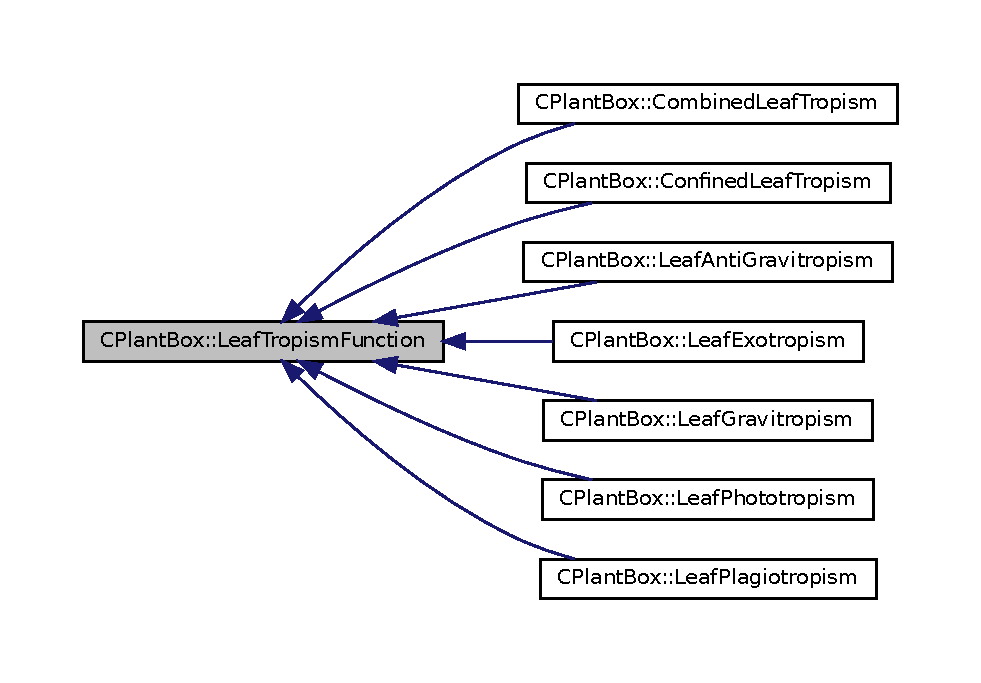
\includegraphics[width=350pt]{classCPlantBox_1_1LeafTropismFunction__inherit__graph}
\end{center}
\end{figure}
\subsection*{Public Member Functions}
\begin{DoxyCompactItemize}
\item 
\hyperlink{classCPlantBox_1_1LeafTropismFunction_ad6f1d7478d104e20cd210fb69dee0d74}{Leaf\+Tropism\+Function} (double n\+\_\+, double sigma\+\_\+)
\item 
\hyperlink{classCPlantBox_1_1LeafTropismFunction_ab5227b152c52aff90ce8d267c71c401a}{Leaf\+Tropism\+Function} ()
\begin{DoxyCompactList}\small\item\em Tropism with n\+\_\+ number of trials and standard deviation of sigma\+\_\+. \end{DoxyCompactList}\item 
virtual \hyperlink{classCPlantBox_1_1Vector2d}{Vector2d} \hyperlink{classCPlantBox_1_1LeafTropismFunction_a1440868221a834474e34e3a503a74572}{get\+Heading} (const \hyperlink{classCPlantBox_1_1Vector3d}{Vector3d} \&pos, \hyperlink{classCPlantBox_1_1Matrix3d}{Matrix3d} old, double dx, const \hyperlink{classCPlantBox_1_1Organ}{Organ} $\ast$leaf)
\begin{DoxyCompactList}\small\item\em Dices n times and takes the best shot (according to the objective function) \end{DoxyCompactList}\item 
virtual double \hyperlink{classCPlantBox_1_1LeafTropismFunction_ab89f5f7e80103d80681bc8cadc220dba}{leaftropism\+Objective} (const \hyperlink{classCPlantBox_1_1Vector3d}{Vector3d} \&pos, \hyperlink{classCPlantBox_1_1Matrix3d}{Matrix3d} old, double a, double b, double dx, const \hyperlink{classCPlantBox_1_1Organ}{Organ} $\ast$leaf)
\begin{DoxyCompactList}\small\item\em The objective function of the random optimization of \hyperlink{classCPlantBox_1_1LeafTropismFunction_a1440868221a834474e34e3a503a74572}{get\+Heading()}. \end{DoxyCompactList}\item 
\mbox{\Hypertarget{classCPlantBox_1_1LeafTropismFunction_a2d47f2a066887cb96dcff5ef440d3400}\label{classCPlantBox_1_1LeafTropismFunction_a2d47f2a066887cb96dcff5ef440d3400}} 
void \hyperlink{classCPlantBox_1_1LeafTropismFunction_a2d47f2a066887cb96dcff5ef440d3400}{set\+Seed} (double seed)
\begin{DoxyCompactList}\small\item\em Sets the seed of the random number generator. \end{DoxyCompactList}\item 
\mbox{\Hypertarget{classCPlantBox_1_1LeafTropismFunction_abedbb803bbcbaea767191a69072c0329}\label{classCPlantBox_1_1LeafTropismFunction_abedbb803bbcbaea767191a69072c0329}} 
double \hyperlink{classCPlantBox_1_1LeafTropismFunction_abedbb803bbcbaea767191a69072c0329}{rand} ()
\begin{DoxyCompactList}\small\item\em Uniformly distributed random number (0,1) \end{DoxyCompactList}\item 
\mbox{\Hypertarget{classCPlantBox_1_1LeafTropismFunction_a841eba2b5f8e9766df7929181a10c5d8}\label{classCPlantBox_1_1LeafTropismFunction_a841eba2b5f8e9766df7929181a10c5d8}} 
double \hyperlink{classCPlantBox_1_1LeafTropismFunction_a841eba2b5f8e9766df7929181a10c5d8}{randn} ()
\begin{DoxyCompactList}\small\item\em Normally distributed random number (0,1) \end{DoxyCompactList}\end{DoxyCompactItemize}
\subsection*{Static Public Member Functions}
\begin{DoxyCompactItemize}
\item 
static \hyperlink{classCPlantBox_1_1Vector3d}{Vector3d} \hyperlink{classCPlantBox_1_1LeafTropismFunction_a87441633ac10289ad861a08a7bf2c411}{get\+Position} (const \hyperlink{classCPlantBox_1_1Vector3d}{Vector3d} \&pos, \hyperlink{classCPlantBox_1_1Matrix3d}{Matrix3d} old, double a, double b, double dx)
\end{DoxyCompactItemize}
\subsection*{Protected Attributes}
\begin{DoxyCompactItemize}
\item 
\mbox{\Hypertarget{classCPlantBox_1_1LeafTropismFunction_a21d8d756f8b9f6015b546def33b01c89}\label{classCPlantBox_1_1LeafTropismFunction_a21d8d756f8b9f6015b546def33b01c89}} 
double \hyperlink{classCPlantBox_1_1LeafTropismFunction_a21d8d756f8b9f6015b546def33b01c89}{n}
\begin{DoxyCompactList}\small\item\em Number of trials. \end{DoxyCompactList}\item 
\mbox{\Hypertarget{classCPlantBox_1_1LeafTropismFunction_a82a3dc11056a65501bc4535749c304b6}\label{classCPlantBox_1_1LeafTropismFunction_a82a3dc11056a65501bc4535749c304b6}} 
double \hyperlink{classCPlantBox_1_1LeafTropismFunction_a82a3dc11056a65501bc4535749c304b6}{sigma}
\begin{DoxyCompactList}\small\item\em Standard deviation. \end{DoxyCompactList}\end{DoxyCompactItemize}


\subsection{Detailed Description}
Base class for all tropism functions, e.\+g. \hyperlink{classCPlantBox_1_1Gravitropism}{Gravitropism}, \hyperlink{classCPlantBox_1_1Plagiotropism}{Plagiotropism}, \hyperlink{classCPlantBox_1_1Exotropism}{Exotropism}... 

\subsection{Constructor \& Destructor Documentation}
\mbox{\Hypertarget{classCPlantBox_1_1LeafTropismFunction_ad6f1d7478d104e20cd210fb69dee0d74}\label{classCPlantBox_1_1LeafTropismFunction_ad6f1d7478d104e20cd210fb69dee0d74}} 
\index{C\+Plant\+Box\+::\+Leaf\+Tropism\+Function@{C\+Plant\+Box\+::\+Leaf\+Tropism\+Function}!Leaf\+Tropism\+Function@{Leaf\+Tropism\+Function}}
\index{Leaf\+Tropism\+Function@{Leaf\+Tropism\+Function}!C\+Plant\+Box\+::\+Leaf\+Tropism\+Function@{C\+Plant\+Box\+::\+Leaf\+Tropism\+Function}}
\subsubsection{\texorpdfstring{Leaf\+Tropism\+Function()}{LeafTropismFunction()}\hspace{0.1cm}{\footnotesize\ttfamily [1/2]}}
{\footnotesize\ttfamily C\+Plant\+Box\+::\+Leaf\+Tropism\+Function\+::\+Leaf\+Tropism\+Function (\begin{DoxyParamCaption}\item[{double}]{n\+\_\+,  }\item[{double}]{sigma\+\_\+ }\end{DoxyParamCaption})\hspace{0.3cm}{\ttfamily [inline]}}

Constructor, Always call the constructor, when overwriting the class! Otherwise it will not work, and the mistake is hard to find.


\begin{DoxyParams}{Parameters}
{\em n\+\_\+} & number of tries \\
\hline
{\em sigma\+\_\+} & standard deviation of angular change \mbox{[}1/cm\mbox{]} \\
\hline
\end{DoxyParams}
\mbox{\Hypertarget{classCPlantBox_1_1LeafTropismFunction_ab5227b152c52aff90ce8d267c71c401a}\label{classCPlantBox_1_1LeafTropismFunction_ab5227b152c52aff90ce8d267c71c401a}} 
\index{C\+Plant\+Box\+::\+Leaf\+Tropism\+Function@{C\+Plant\+Box\+::\+Leaf\+Tropism\+Function}!Leaf\+Tropism\+Function@{Leaf\+Tropism\+Function}}
\index{Leaf\+Tropism\+Function@{Leaf\+Tropism\+Function}!C\+Plant\+Box\+::\+Leaf\+Tropism\+Function@{C\+Plant\+Box\+::\+Leaf\+Tropism\+Function}}
\subsubsection{\texorpdfstring{Leaf\+Tropism\+Function()}{LeafTropismFunction()}\hspace{0.1cm}{\footnotesize\ttfamily [2/2]}}
{\footnotesize\ttfamily C\+Plant\+Box\+::\+Leaf\+Tropism\+Function\+::\+Leaf\+Tropism\+Function (\begin{DoxyParamCaption}{ }\end{DoxyParamCaption})\hspace{0.3cm}{\ttfamily [inline]}}



Tropism with n\+\_\+ number of trials and standard deviation of sigma\+\_\+. 

Default constructor is Tropism\+Function(0,0) 

\subsection{Member Function Documentation}
\mbox{\Hypertarget{classCPlantBox_1_1LeafTropismFunction_a1440868221a834474e34e3a503a74572}\label{classCPlantBox_1_1LeafTropismFunction_a1440868221a834474e34e3a503a74572}} 
\index{C\+Plant\+Box\+::\+Leaf\+Tropism\+Function@{C\+Plant\+Box\+::\+Leaf\+Tropism\+Function}!get\+Heading@{get\+Heading}}
\index{get\+Heading@{get\+Heading}!C\+Plant\+Box\+::\+Leaf\+Tropism\+Function@{C\+Plant\+Box\+::\+Leaf\+Tropism\+Function}}
\subsubsection{\texorpdfstring{get\+Heading()}{getHeading()}}
{\footnotesize\ttfamily \hyperlink{classCPlantBox_1_1Vector2d}{Vector2d} C\+Plant\+Box\+::\+Leaf\+Tropism\+Function\+::get\+Heading (\begin{DoxyParamCaption}\item[{const \hyperlink{classCPlantBox_1_1Vector3d}{Vector3d} \&}]{pos,  }\item[{\hyperlink{classCPlantBox_1_1Matrix3d}{Matrix3d}}]{old,  }\item[{double}]{dx,  }\item[{const \hyperlink{classCPlantBox_1_1Organ}{Organ} $\ast$}]{leaf }\end{DoxyParamCaption})\hspace{0.3cm}{\ttfamily [virtual]}}



Dices n times and takes the best shot (according to the objective function) 

-\/-\/-\/-\/-\/-\/-\/-\/-\/-\/-\/-\/-\/-\/-\/-\/-\/-\/-\/-\/-\/-\/-\/-\/-\/-\/-\/-\/-\/-\/-\/-\/-\/-\/-\/-\/-\/-\/-\/-\/-\/-\/-\/-\/-\/-\/-\/-\/-\/-\/-\/-\/-\/-\/---------Tropism Modified and Used-\/-\/-\/-\/-\/-\/-\/-\/-\/-\/-\/-\/-\/-\/-\/-\/-\/-\/-\/-\/-\/-\/-\/-\/-\/-\/-\/-\/-\/-\/-\/-\/-\/-\/-\/-\/-\/-\/-\/-\/-\/-\/-\/-\/-\/-\/-\/-\/-\/-\/-\/-\/-\/---------///

Dices N times picking angles alpha and beta, takes the optimal direction according to the objective function


\begin{DoxyParams}{Parameters}
{\em pos} & root tip position \\
\hline
{\em old} & rotation matrix, heading is old(\+:,1) \\
\hline
{\em dx} & distance to look ahead (e.\+g in case of hydrotropism) \\
\hline
{\em root} & points to the root that called get\+Heading(...), just in case something else is needed (i.\+e. iheading for exotropism)\\
\hline
\end{DoxyParams}
\begin{DoxyReturn}{Returns}
angle alpha and beta 
\end{DoxyReturn}
\hyperlink{classCPlantBox_1_1LeafTropismFunction_abedbb803bbcbaea767191a69072c0329}{rand()}$\ast$2$\ast$\+M\+\_\+\+PI;

sigma$\ast$randn()$\ast$sqrt(dx); 

Reimplemented in \hyperlink{classCPlantBox_1_1ConfinedLeafTropism_a0574aa544341937fc9df37a972cd0833}{C\+Plant\+Box\+::\+Confined\+Leaf\+Tropism}.

\mbox{\Hypertarget{classCPlantBox_1_1LeafTropismFunction_a87441633ac10289ad861a08a7bf2c411}\label{classCPlantBox_1_1LeafTropismFunction_a87441633ac10289ad861a08a7bf2c411}} 
\index{C\+Plant\+Box\+::\+Leaf\+Tropism\+Function@{C\+Plant\+Box\+::\+Leaf\+Tropism\+Function}!get\+Position@{get\+Position}}
\index{get\+Position@{get\+Position}!C\+Plant\+Box\+::\+Leaf\+Tropism\+Function@{C\+Plant\+Box\+::\+Leaf\+Tropism\+Function}}
\subsubsection{\texorpdfstring{get\+Position()}{getPosition()}}
{\footnotesize\ttfamily \hyperlink{classCPlantBox_1_1Vector3d}{Vector3d} C\+Plant\+Box\+::\+Leaf\+Tropism\+Function\+::get\+Position (\begin{DoxyParamCaption}\item[{const \hyperlink{classCPlantBox_1_1Vector3d}{Vector3d} \&}]{pos,  }\item[{\hyperlink{classCPlantBox_1_1Matrix3d}{Matrix3d}}]{old,  }\item[{double}]{a,  }\item[{double}]{b,  }\item[{double}]{dx }\end{DoxyParamCaption})\hspace{0.3cm}{\ttfamily [static]}}

Applies angles a and b and goes dx \mbox{[}cm\mbox{]} into the new direction and returns the new position


\begin{DoxyParams}{Parameters}
{\em pos} & root tip position \\
\hline
{\em old} & rotation matrix, heading is old(\+:,1) \\
\hline
{\em a} & angle alpha, describes the angular rotation of the axis old \\
\hline
{\em b} & angle beta, describes the radial rotation of the axis old \\
\hline
{\em dx} & distance to look ahead\\
\hline
\end{DoxyParams}
\begin{DoxyReturn}{Returns}
position 
\end{DoxyReturn}
\mbox{\Hypertarget{classCPlantBox_1_1LeafTropismFunction_ab89f5f7e80103d80681bc8cadc220dba}\label{classCPlantBox_1_1LeafTropismFunction_ab89f5f7e80103d80681bc8cadc220dba}} 
\index{C\+Plant\+Box\+::\+Leaf\+Tropism\+Function@{C\+Plant\+Box\+::\+Leaf\+Tropism\+Function}!leaftropism\+Objective@{leaftropism\+Objective}}
\index{leaftropism\+Objective@{leaftropism\+Objective}!C\+Plant\+Box\+::\+Leaf\+Tropism\+Function@{C\+Plant\+Box\+::\+Leaf\+Tropism\+Function}}
\subsubsection{\texorpdfstring{leaftropism\+Objective()}{leaftropismObjective()}}
{\footnotesize\ttfamily virtual double C\+Plant\+Box\+::\+Leaf\+Tropism\+Function\+::leaftropism\+Objective (\begin{DoxyParamCaption}\item[{const \hyperlink{classCPlantBox_1_1Vector3d}{Vector3d} \&}]{pos,  }\item[{\hyperlink{classCPlantBox_1_1Matrix3d}{Matrix3d}}]{old,  }\item[{double}]{a,  }\item[{double}]{b,  }\item[{double}]{dx,  }\item[{const \hyperlink{classCPlantBox_1_1Organ}{Organ} $\ast$}]{leaf }\end{DoxyParamCaption})\hspace{0.3cm}{\ttfamily [inline]}, {\ttfamily [virtual]}}



The objective function of the random optimization of \hyperlink{classCPlantBox_1_1LeafTropismFunction_a1440868221a834474e34e3a503a74572}{get\+Heading()}. 

The objective function of the random optimization of \hyperlink{classCPlantBox_1_1LeafTropismFunction_a1440868221a834474e34e3a503a74572}{get\+Heading()}. Overwrite this function to implement a tropism.


\begin{DoxyParams}{Parameters}
{\em pos} & current root tip position \\
\hline
{\em old} & rotation matrix, old(\+:,1) is the root tip heading \\
\hline
{\em a} & rotation angle alpha (angular change) \\
\hline
{\em b} & rotation angle beta (radial change) \\
\hline
{\em dx} & small ditance to look ahead \\
\hline
{\em root} & points to the root that called get\+Heading, just in case something else is needed (i.\+e. iheading for exotropism)\\
\hline
\end{DoxyParams}
\begin{DoxyReturn}{Returns}
the value minimized by \hyperlink{classCPlantBox_1_1LeafTropismFunction_a1440868221a834474e34e3a503a74572}{get\+Heading()}, it should be in \mbox{[}0,1\mbox{]}, in this way combination of various tropisms will be easier 
\end{DoxyReturn}


Reimplemented in \hyperlink{classCPlantBox_1_1CombinedLeafTropism_aec7a53f31265f6c10a8666d0d8647aa5}{C\+Plant\+Box\+::\+Combined\+Leaf\+Tropism}, \hyperlink{classCPlantBox_1_1LeafPhototropism_a9b9cee624adc576c2cc44b1b27b2ef0c}{C\+Plant\+Box\+::\+Leaf\+Phototropism}, \hyperlink{classCPlantBox_1_1LeafExotropism_a0b3820189c2cef88d32a0d8130c15246}{C\+Plant\+Box\+::\+Leaf\+Exotropism}, \hyperlink{classCPlantBox_1_1LeafPlagiotropism_af58514b24aae9a1020093d6955dadaaf}{C\+Plant\+Box\+::\+Leaf\+Plagiotropism}, \hyperlink{classCPlantBox_1_1LeafAntiGravitropism_a94f4abfb99515326081deebff7906ca2}{C\+Plant\+Box\+::\+Leaf\+Anti\+Gravitropism}, \hyperlink{classCPlantBox_1_1LeafGravitropism_ab0836658683f5364fef25bafc7ac610e}{C\+Plant\+Box\+::\+Leaf\+Gravitropism}, and \hyperlink{classCPlantBox_1_1ConfinedLeafTropism_afaa130b76e027bd9c21fe1938ecf9067}{C\+Plant\+Box\+::\+Confined\+Leaf\+Tropism}.



The documentation for this class was generated from the following files\+:\begin{DoxyCompactItemize}
\item 
src/Leaf\+Tropism.\+h\item 
src/Leaf\+Tropism.\+cpp\end{DoxyCompactItemize}

\hypertarget{classCPlantBox_1_1LinearGrowth}{}\section{C\+Plant\+Box\+:\+:Linear\+Growth Class Reference}
\label{classCPlantBox_1_1LinearGrowth}\index{C\+Plant\+Box\+::\+Linear\+Growth@{C\+Plant\+Box\+::\+Linear\+Growth}}


{\ttfamily \#include $<$Root\+Growth.\+h$>$}



Inheritance diagram for C\+Plant\+Box\+:\+:Linear\+Growth\+:\nopagebreak
\begin{figure}[H]
\begin{center}
\leavevmode
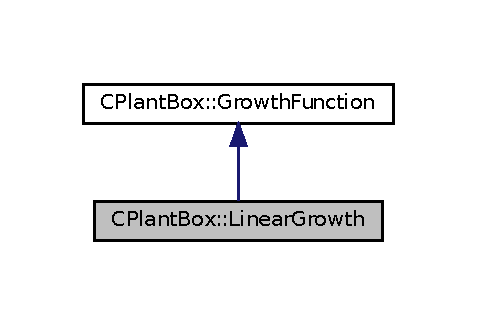
\includegraphics[width=229pt]{classCPlantBox_1_1LinearGrowth__inherit__graph}
\end{center}
\end{figure}


Collaboration diagram for C\+Plant\+Box\+:\+:Linear\+Growth\+:\nopagebreak
\begin{figure}[H]
\begin{center}
\leavevmode
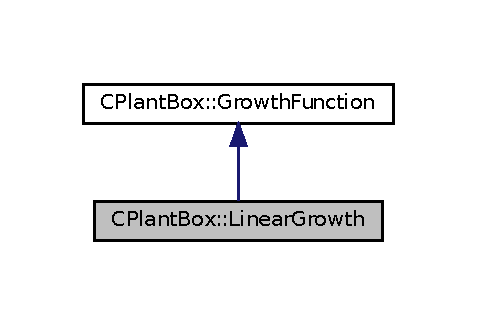
\includegraphics[width=229pt]{classCPlantBox_1_1LinearGrowth__coll__graph}
\end{center}
\end{figure}
\subsection*{Public Member Functions}
\begin{DoxyCompactItemize}
\item 
virtual double \hyperlink{classCPlantBox_1_1LinearGrowth_afffda4dacad7cd28f6addb6d3268cf1f}{get\+Length} (double t, double r, double k, \hyperlink{classCPlantBox_1_1Organ}{Organ} $\ast$root) const
\item 
virtual double \hyperlink{classCPlantBox_1_1LinearGrowth_a7880e35aa61d276647d9a602775dd87a}{get\+Age} (double l, double r, double k, \hyperlink{classCPlantBox_1_1Organ}{Organ} $\ast$root) const
\end{DoxyCompactItemize}


\subsection{Detailed Description}
\hyperlink{classCPlantBox_1_1LinearGrowth}{Linear\+Growth} elongates at constant rate until the maximal length k is reached 

\subsection{Member Function Documentation}
\mbox{\Hypertarget{classCPlantBox_1_1LinearGrowth_a7880e35aa61d276647d9a602775dd87a}\label{classCPlantBox_1_1LinearGrowth_a7880e35aa61d276647d9a602775dd87a}} 
\index{C\+Plant\+Box\+::\+Linear\+Growth@{C\+Plant\+Box\+::\+Linear\+Growth}!get\+Age@{get\+Age}}
\index{get\+Age@{get\+Age}!C\+Plant\+Box\+::\+Linear\+Growth@{C\+Plant\+Box\+::\+Linear\+Growth}}
\subsubsection{\texorpdfstring{get\+Age()}{getAge()}}
{\footnotesize\ttfamily virtual double C\+Plant\+Box\+::\+Linear\+Growth\+::get\+Age (\begin{DoxyParamCaption}\item[{double}]{l,  }\item[{double}]{r,  }\item[{double}]{k,  }\item[{\hyperlink{classCPlantBox_1_1Organ}{Organ} $\ast$}]{root }\end{DoxyParamCaption}) const\hspace{0.3cm}{\ttfamily [inline]}, {\ttfamily [virtual]}}

\begin{DoxySeeAlso}{See also}
\hyperlink{classCPlantBox_1_1GrowthFunction}{Growth\+Function} 
\end{DoxySeeAlso}


Reimplemented from \hyperlink{classCPlantBox_1_1GrowthFunction_a006b428760c410389afa54853fe7cc1f}{C\+Plant\+Box\+::\+Growth\+Function}.

\mbox{\Hypertarget{classCPlantBox_1_1LinearGrowth_afffda4dacad7cd28f6addb6d3268cf1f}\label{classCPlantBox_1_1LinearGrowth_afffda4dacad7cd28f6addb6d3268cf1f}} 
\index{C\+Plant\+Box\+::\+Linear\+Growth@{C\+Plant\+Box\+::\+Linear\+Growth}!get\+Length@{get\+Length}}
\index{get\+Length@{get\+Length}!C\+Plant\+Box\+::\+Linear\+Growth@{C\+Plant\+Box\+::\+Linear\+Growth}}
\subsubsection{\texorpdfstring{get\+Length()}{getLength()}}
{\footnotesize\ttfamily virtual double C\+Plant\+Box\+::\+Linear\+Growth\+::get\+Length (\begin{DoxyParamCaption}\item[{double}]{t,  }\item[{double}]{r,  }\item[{double}]{k,  }\item[{\hyperlink{classCPlantBox_1_1Organ}{Organ} $\ast$}]{root }\end{DoxyParamCaption}) const\hspace{0.3cm}{\ttfamily [inline]}, {\ttfamily [virtual]}}

\begin{DoxySeeAlso}{See also}
\hyperlink{classCPlantBox_1_1GrowthFunction}{Growth\+Function} 
\end{DoxySeeAlso}


Reimplemented from \hyperlink{classCPlantBox_1_1GrowthFunction_a41b83da5d75beab49846c5b92a421e43}{C\+Plant\+Box\+::\+Growth\+Function}.



The documentation for this class was generated from the following file\+:\begin{DoxyCompactItemize}
\item 
src/Root\+Growth.\+h\end{DoxyCompactItemize}

\hypertarget{structCPlantBox_1_1tinyxml2_1_1LongFitsIntoSizeTMinusOne}{}\section{C\+Plant\+Box\+:\+:tinyxml2\+:\+:Long\+Fits\+Into\+Size\+T\+Minus\+One$<$ bool $>$ Struct Template Reference}
\label{structCPlantBox_1_1tinyxml2_1_1LongFitsIntoSizeTMinusOne}\index{C\+Plant\+Box\+::tinyxml2\+::\+Long\+Fits\+Into\+Size\+T\+Minus\+One$<$ bool $>$@{C\+Plant\+Box\+::tinyxml2\+::\+Long\+Fits\+Into\+Size\+T\+Minus\+One$<$ bool $>$}}
\subsection*{Static Public Member Functions}
\begin{DoxyCompactItemize}
\item 
\mbox{\Hypertarget{structCPlantBox_1_1tinyxml2_1_1LongFitsIntoSizeTMinusOne_a5c4266da0936711eddc0689ab4f8a7cd}\label{structCPlantBox_1_1tinyxml2_1_1LongFitsIntoSizeTMinusOne_a5c4266da0936711eddc0689ab4f8a7cd}} 
static bool {\bfseries Fits} (unsigned long value)
\end{DoxyCompactItemize}


The documentation for this struct was generated from the following file\+:\begin{DoxyCompactItemize}
\item 
src/tinyxml2.\+cpp\end{DoxyCompactItemize}

\hypertarget{structCPlantBox_1_1tinyxml2_1_1LongFitsIntoSizeTMinusOne_3_01false_01_4}{}\section{C\+Plant\+Box\+:\+:tinyxml2\+:\+:Long\+Fits\+Into\+Size\+T\+Minus\+One$<$ false $>$ Struct Template Reference}
\label{structCPlantBox_1_1tinyxml2_1_1LongFitsIntoSizeTMinusOne_3_01false_01_4}\index{C\+Plant\+Box\+::tinyxml2\+::\+Long\+Fits\+Into\+Size\+T\+Minus\+One$<$ false $>$@{C\+Plant\+Box\+::tinyxml2\+::\+Long\+Fits\+Into\+Size\+T\+Minus\+One$<$ false $>$}}
\subsection*{Static Public Member Functions}
\begin{DoxyCompactItemize}
\item 
\mbox{\Hypertarget{structCPlantBox_1_1tinyxml2_1_1LongFitsIntoSizeTMinusOne_3_01false_01_4_a8d213de91cf20b2bb6a8b2b70d0d6d5d}\label{structCPlantBox_1_1tinyxml2_1_1LongFitsIntoSizeTMinusOne_3_01false_01_4_a8d213de91cf20b2bb6a8b2b70d0d6d5d}} 
static bool {\bfseries Fits} (unsigned long)
\end{DoxyCompactItemize}


The documentation for this struct was generated from the following file\+:\begin{DoxyCompactItemize}
\item 
src/tinyxml2.\+cpp\end{DoxyCompactItemize}

\hypertarget{classCPlantBox_1_1Matrix3d}{}\section{C\+Plant\+Box\+:\+:Matrix3d Class Reference}
\label{classCPlantBox_1_1Matrix3d}\index{C\+Plant\+Box\+::\+Matrix3d@{C\+Plant\+Box\+::\+Matrix3d}}


{\ttfamily \#include $<$mymath.\+h$>$}



Collaboration diagram for C\+Plant\+Box\+:\+:Matrix3d\+:\nopagebreak
\begin{figure}[H]
\begin{center}
\leavevmode
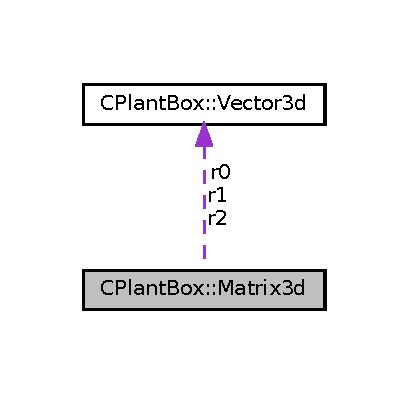
\includegraphics[width=196pt]{classCPlantBox_1_1Matrix3d__coll__graph}
\end{center}
\end{figure}
\subsection*{Public Member Functions}
\begin{DoxyCompactItemize}
\item 
\mbox{\Hypertarget{classCPlantBox_1_1Matrix3d_aba20b85af0ce770d0ac0aba44b7ebb94}\label{classCPlantBox_1_1Matrix3d_aba20b85af0ce770d0ac0aba44b7ebb94}} 
\hyperlink{classCPlantBox_1_1Matrix3d_aba20b85af0ce770d0ac0aba44b7ebb94}{Matrix3d} ()
\begin{DoxyCompactList}\small\item\em Default constructor (identity matrix) \end{DoxyCompactList}\item 
\mbox{\Hypertarget{classCPlantBox_1_1Matrix3d_a1a0f7c0db69375fbaf99f7354366d5da}\label{classCPlantBox_1_1Matrix3d_a1a0f7c0db69375fbaf99f7354366d5da}} 
\hyperlink{classCPlantBox_1_1Matrix3d_a1a0f7c0db69375fbaf99f7354366d5da}{Matrix3d} (double m11, double m12, double m13, double m21, double m22, double m23, double m31, double m32, double m33)
\begin{DoxyCompactList}\small\item\em Constructor passing nine doubles as 3x3 matrix entries. \end{DoxyCompactList}\item 
\mbox{\Hypertarget{classCPlantBox_1_1Matrix3d_a660dff2581b4f427acfff025f7655fc7}\label{classCPlantBox_1_1Matrix3d_a660dff2581b4f427acfff025f7655fc7}} 
\hyperlink{classCPlantBox_1_1Matrix3d_a660dff2581b4f427acfff025f7655fc7}{Matrix3d} (const \hyperlink{classCPlantBox_1_1Vector3d}{Vector3d} \&c1, const \hyperlink{classCPlantBox_1_1Vector3d}{Vector3d} \&c2, const \hyperlink{classCPlantBox_1_1Vector3d}{Vector3d} \&c3)
\begin{DoxyCompactList}\small\item\em Constructs the matrix from three column vectors. \end{DoxyCompactList}\item 
\mbox{\Hypertarget{classCPlantBox_1_1Matrix3d_af7de6b14f07dc9d6968a53d3ef14c360}\label{classCPlantBox_1_1Matrix3d_af7de6b14f07dc9d6968a53d3ef14c360}} 
\hyperlink{classCPlantBox_1_1Matrix3d_af7de6b14f07dc9d6968a53d3ef14c360}{Matrix3d} (const \hyperlink{classCPlantBox_1_1Matrix3d}{Matrix3d} \&m)
\begin{DoxyCompactList}\small\item\em Copy constructor. \end{DoxyCompactList}\item 
\mbox{\Hypertarget{classCPlantBox_1_1Matrix3d_a1e695998373d052aeae94cccd8b7fa16}\label{classCPlantBox_1_1Matrix3d_a1e695998373d052aeae94cccd8b7fa16}} 
double \hyperlink{classCPlantBox_1_1Matrix3d_a1e695998373d052aeae94cccd8b7fa16}{det} () const
\begin{DoxyCompactList}\small\item\em determinant of the matrix \end{DoxyCompactList}\item 
\mbox{\Hypertarget{classCPlantBox_1_1Matrix3d_a6b51e2a2d5ca24cd5199ac0c4990fb44}\label{classCPlantBox_1_1Matrix3d_a6b51e2a2d5ca24cd5199ac0c4990fb44}} 
\hyperlink{classCPlantBox_1_1Matrix3d}{Matrix3d} \hyperlink{classCPlantBox_1_1Matrix3d_a6b51e2a2d5ca24cd5199ac0c4990fb44}{inverse} () const
\begin{DoxyCompactList}\small\item\em calculates the inverse of the matrix \end{DoxyCompactList}\item 
\mbox{\Hypertarget{classCPlantBox_1_1Matrix3d_a4db104d3e5afe1b5737a26f70663a595}\label{classCPlantBox_1_1Matrix3d_a4db104d3e5afe1b5737a26f70663a595}} 
\hyperlink{classCPlantBox_1_1Vector3d}{Vector3d} \hyperlink{classCPlantBox_1_1Matrix3d_a4db104d3e5afe1b5737a26f70663a595}{column} (int i) const
\begin{DoxyCompactList}\small\item\em returns the i-\/th column of the matrix (i=0..2) \end{DoxyCompactList}\item 
\mbox{\Hypertarget{classCPlantBox_1_1Matrix3d_ae015fb90aa09bafd9f3dde759dd5642d}\label{classCPlantBox_1_1Matrix3d_ae015fb90aa09bafd9f3dde759dd5642d}} 
\hyperlink{classCPlantBox_1_1Vector3d}{Vector3d} \hyperlink{classCPlantBox_1_1Matrix3d_ae015fb90aa09bafd9f3dde759dd5642d}{row} (int i) const
\begin{DoxyCompactList}\small\item\em returns the i-\/th row of the matrix (i=0..2) \end{DoxyCompactList}\item 
\mbox{\Hypertarget{classCPlantBox_1_1Matrix3d_aff198f7d945f7b429932678e21b5b62b}\label{classCPlantBox_1_1Matrix3d_aff198f7d945f7b429932678e21b5b62b}} 
void \hyperlink{classCPlantBox_1_1Matrix3d_aff198f7d945f7b429932678e21b5b62b}{times} (const \hyperlink{classCPlantBox_1_1Matrix3d}{Matrix3d} \&m)
\begin{DoxyCompactList}\small\item\em Multiplies matrix m from right. \end{DoxyCompactList}\item 
\mbox{\Hypertarget{classCPlantBox_1_1Matrix3d_afc3f908f0e56f1a7b377857dbf8bb5af}\label{classCPlantBox_1_1Matrix3d_afc3f908f0e56f1a7b377857dbf8bb5af}} 
\hyperlink{classCPlantBox_1_1Vector3d}{Vector3d} \hyperlink{classCPlantBox_1_1Matrix3d_afc3f908f0e56f1a7b377857dbf8bb5af}{times} (const \hyperlink{classCPlantBox_1_1Vector3d}{Vector3d} \&v) const
\begin{DoxyCompactList}\small\item\em Multiplies vector v from right. \end{DoxyCompactList}\item 
\mbox{\Hypertarget{classCPlantBox_1_1Matrix3d_a7843cea2ad51b889eed45f7892aec1f5}\label{classCPlantBox_1_1Matrix3d_a7843cea2ad51b889eed45f7892aec1f5}} 
std\+::string \hyperlink{classCPlantBox_1_1Matrix3d_a7843cea2ad51b889eed45f7892aec1f5}{to\+String} () const
\begin{DoxyCompactList}\small\item\em creates a string representing the 3x3 matrix \end{DoxyCompactList}\end{DoxyCompactItemize}
\subsection*{Static Public Member Functions}
\begin{DoxyCompactItemize}
\item 
\mbox{\Hypertarget{classCPlantBox_1_1Matrix3d_a8895aef9fc0ba32151a046247f10766f}\label{classCPlantBox_1_1Matrix3d_a8895aef9fc0ba32151a046247f10766f}} 
static \hyperlink{classCPlantBox_1_1Matrix3d}{Matrix3d} \hyperlink{classCPlantBox_1_1Matrix3d_a8895aef9fc0ba32151a046247f10766f}{rotX} (double a)
\begin{DoxyCompactList}\small\item\em Creates a rotation matrix around the X-\/axis. \end{DoxyCompactList}\item 
\mbox{\Hypertarget{classCPlantBox_1_1Matrix3d_abaf49f5d175678190505ad23e74e53e7}\label{classCPlantBox_1_1Matrix3d_abaf49f5d175678190505ad23e74e53e7}} 
static \hyperlink{classCPlantBox_1_1Matrix3d}{Matrix3d} \hyperlink{classCPlantBox_1_1Matrix3d_abaf49f5d175678190505ad23e74e53e7}{rotY} (double a)
\begin{DoxyCompactList}\small\item\em Creates a rotation matrix around the Y-\/axis. \end{DoxyCompactList}\item 
\mbox{\Hypertarget{classCPlantBox_1_1Matrix3d_aed1b8c6635dde507caf90d01eb5e02d4}\label{classCPlantBox_1_1Matrix3d_aed1b8c6635dde507caf90d01eb5e02d4}} 
static \hyperlink{classCPlantBox_1_1Matrix3d}{Matrix3d} \hyperlink{classCPlantBox_1_1Matrix3d_aed1b8c6635dde507caf90d01eb5e02d4}{rotZ} (double a)
\begin{DoxyCompactList}\small\item\em Creates a rotation matrix around the Z-\/axis. \end{DoxyCompactList}\item 
static \hyperlink{classCPlantBox_1_1Matrix3d}{Matrix3d} \hyperlink{classCPlantBox_1_1Matrix3d_a65224dd4969719c7fc8072c6a913f4c8}{ons} (\hyperlink{classCPlantBox_1_1Vector3d}{Vector3d} \&v, int vec\+\_\+pos=0)
\begin{DoxyCompactList}\small\item\em Creates an orthonormal system (O\+NS) around the vector v. \end{DoxyCompactList}\end{DoxyCompactItemize}
\subsection*{Public Attributes}
\begin{DoxyCompactItemize}
\item 
\mbox{\Hypertarget{classCPlantBox_1_1Matrix3d_ab35ef40d84f9ee9ec992e0f7868c6edf}\label{classCPlantBox_1_1Matrix3d_ab35ef40d84f9ee9ec992e0f7868c6edf}} 
\hyperlink{classCPlantBox_1_1Vector3d}{Vector3d} \hyperlink{classCPlantBox_1_1Matrix3d_ab35ef40d84f9ee9ec992e0f7868c6edf}{r0}
\begin{DoxyCompactList}\small\item\em row 1 \end{DoxyCompactList}\item 
\mbox{\Hypertarget{classCPlantBox_1_1Matrix3d_a68c25f556d573979743a8ed12adb68ed}\label{classCPlantBox_1_1Matrix3d_a68c25f556d573979743a8ed12adb68ed}} 
\hyperlink{classCPlantBox_1_1Vector3d}{Vector3d} \hyperlink{classCPlantBox_1_1Matrix3d_a68c25f556d573979743a8ed12adb68ed}{r1}
\begin{DoxyCompactList}\small\item\em row 2 \end{DoxyCompactList}\item 
\mbox{\Hypertarget{classCPlantBox_1_1Matrix3d_a426ed493e511b936e0008384db09deca}\label{classCPlantBox_1_1Matrix3d_a426ed493e511b936e0008384db09deca}} 
\hyperlink{classCPlantBox_1_1Vector3d}{Vector3d} \hyperlink{classCPlantBox_1_1Matrix3d_a426ed493e511b936e0008384db09deca}{r2}
\begin{DoxyCompactList}\small\item\em row 3 \end{DoxyCompactList}\end{DoxyCompactItemize}


\subsection{Detailed Description}
3x3 Matrix class, compatible with \hyperlink{classCPlantBox_1_1Vector3d}{Vector3d} for basic linear algebra (i.\+e. exactly the operations needed for C\+Root\+Box) 

\subsection{Member Function Documentation}
\mbox{\Hypertarget{classCPlantBox_1_1Matrix3d_a65224dd4969719c7fc8072c6a913f4c8}\label{classCPlantBox_1_1Matrix3d_a65224dd4969719c7fc8072c6a913f4c8}} 
\index{C\+Plant\+Box\+::\+Matrix3d@{C\+Plant\+Box\+::\+Matrix3d}!ons@{ons}}
\index{ons@{ons}!C\+Plant\+Box\+::\+Matrix3d@{C\+Plant\+Box\+::\+Matrix3d}}
\subsubsection{\texorpdfstring{ons()}{ons()}}
{\footnotesize\ttfamily static \hyperlink{classCPlantBox_1_1Matrix3d}{Matrix3d} C\+Plant\+Box\+::\+Matrix3d\+::ons (\begin{DoxyParamCaption}\item[{\hyperlink{classCPlantBox_1_1Vector3d}{Vector3d} \&}]{v,  }\item[{int}]{vec\+\_\+pos = {\ttfamily 0} }\end{DoxyParamCaption})\hspace{0.3cm}{\ttfamily [inline]}, {\ttfamily [static]}}



Creates an orthonormal system (O\+NS) around the vector v. 

Creates an orthonormal system (O\+NS) around the vector v

Remark\+: This is not unique, in Rootbox the O\+NS is rotated around a random angle to make it truly random. This is likely to be not optimal, but I guess it is fast enough anyway.


\begin{DoxyParams}{Parameters}
{\em v} & vector, that will be normalized and then be the first column of the resulting O\+NS\\
\hline
\end{DoxyParams}
\begin{DoxyReturn}{Returns}
three orthonormal column vectors 
\end{DoxyReturn}


The documentation for this class was generated from the following file\+:\begin{DoxyCompactItemize}
\item 
src/mymath.\+h\end{DoxyCompactItemize}

\hypertarget{classCPlantBox_1_1tinyxml2_1_1MemPool}{}\section{C\+Plant\+Box\+:\+:tinyxml2\+:\+:Mem\+Pool Class Reference}
\label{classCPlantBox_1_1tinyxml2_1_1MemPool}\index{C\+Plant\+Box\+::tinyxml2\+::\+Mem\+Pool@{C\+Plant\+Box\+::tinyxml2\+::\+Mem\+Pool}}


Inheritance diagram for C\+Plant\+Box\+:\+:tinyxml2\+:\+:Mem\+Pool\+:\nopagebreak
\begin{figure}[H]
\begin{center}
\leavevmode
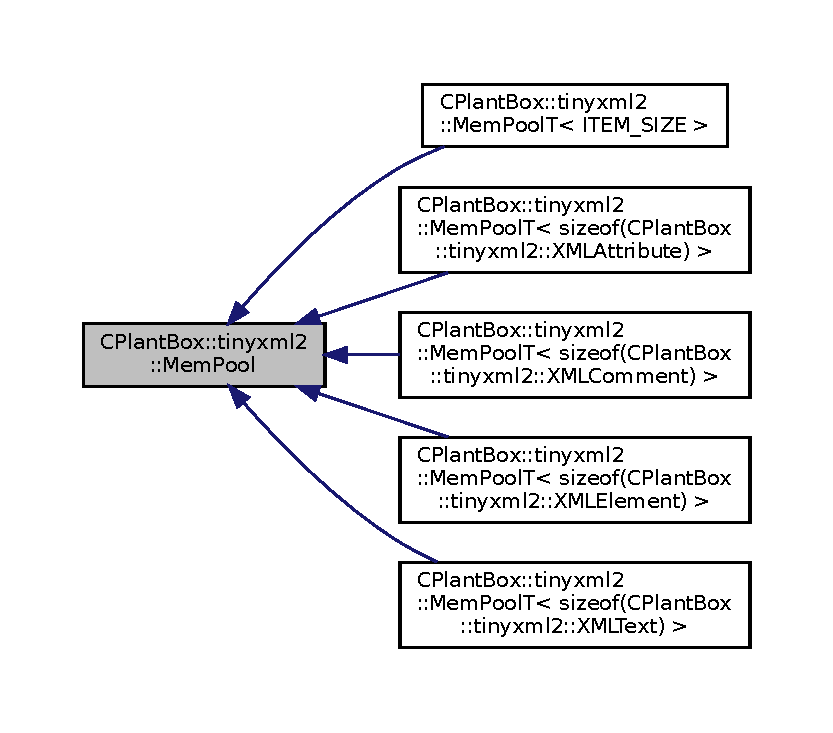
\includegraphics[width=350pt]{classCPlantBox_1_1tinyxml2_1_1MemPool__inherit__graph}
\end{center}
\end{figure}
\subsection*{Public Member Functions}
\begin{DoxyCompactItemize}
\item 
\mbox{\Hypertarget{classCPlantBox_1_1tinyxml2_1_1MemPool_a2a69a5f946316d8c0a8dab2e57a5322b}\label{classCPlantBox_1_1tinyxml2_1_1MemPool_a2a69a5f946316d8c0a8dab2e57a5322b}} 
virtual int {\bfseries Item\+Size} () const =0
\item 
\mbox{\Hypertarget{classCPlantBox_1_1tinyxml2_1_1MemPool_a967f9c5aee7308afcd90a0ed98e5f75f}\label{classCPlantBox_1_1tinyxml2_1_1MemPool_a967f9c5aee7308afcd90a0ed98e5f75f}} 
virtual void $\ast$ {\bfseries Alloc} ()=0
\item 
\mbox{\Hypertarget{classCPlantBox_1_1tinyxml2_1_1MemPool_aff94c5932df6b157fb6e631404d7ad3d}\label{classCPlantBox_1_1tinyxml2_1_1MemPool_aff94c5932df6b157fb6e631404d7ad3d}} 
virtual void {\bfseries Free} (void $\ast$)=0
\item 
\mbox{\Hypertarget{classCPlantBox_1_1tinyxml2_1_1MemPool_aa4e3a16a55d297074a5ad488d2f88798}\label{classCPlantBox_1_1tinyxml2_1_1MemPool_aa4e3a16a55d297074a5ad488d2f88798}} 
virtual void {\bfseries Set\+Tracked} ()=0
\item 
\mbox{\Hypertarget{classCPlantBox_1_1tinyxml2_1_1MemPool_a459afd20c05174056fefbee12002540c}\label{classCPlantBox_1_1tinyxml2_1_1MemPool_a459afd20c05174056fefbee12002540c}} 
virtual void {\bfseries Clear} ()=0
\end{DoxyCompactItemize}


The documentation for this class was generated from the following file\+:\begin{DoxyCompactItemize}
\item 
src/tinyxml2.\+h\end{DoxyCompactItemize}

\hypertarget{classCPlantBox_1_1tinyxml2_1_1MemPoolT}{}\section{C\+Plant\+Box\+:\+:tinyxml2\+:\+:Mem\+PoolT$<$ I\+T\+E\+M\+\_\+\+S\+I\+ZE $>$ Class Template Reference}
\label{classCPlantBox_1_1tinyxml2_1_1MemPoolT}\index{C\+Plant\+Box\+::tinyxml2\+::\+Mem\+Pool\+T$<$ I\+T\+E\+M\+\_\+\+S\+I\+Z\+E $>$@{C\+Plant\+Box\+::tinyxml2\+::\+Mem\+Pool\+T$<$ I\+T\+E\+M\+\_\+\+S\+I\+Z\+E $>$}}


Inheritance diagram for C\+Plant\+Box\+:\+:tinyxml2\+:\+:Mem\+PoolT$<$ I\+T\+E\+M\+\_\+\+S\+I\+ZE $>$\+:\nopagebreak
\begin{figure}[H]
\begin{center}
\leavevmode
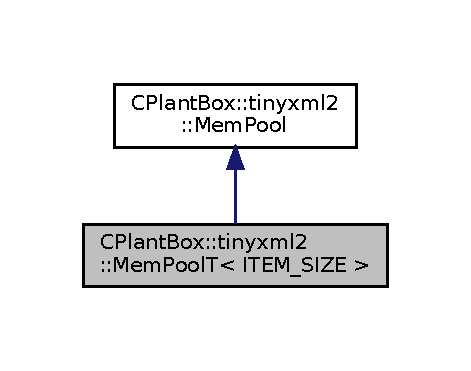
\includegraphics[width=226pt]{classCPlantBox_1_1tinyxml2_1_1MemPoolT__inherit__graph}
\end{center}
\end{figure}


Collaboration diagram for C\+Plant\+Box\+:\+:tinyxml2\+:\+:Mem\+PoolT$<$ I\+T\+E\+M\+\_\+\+S\+I\+ZE $>$\+:\nopagebreak
\begin{figure}[H]
\begin{center}
\leavevmode
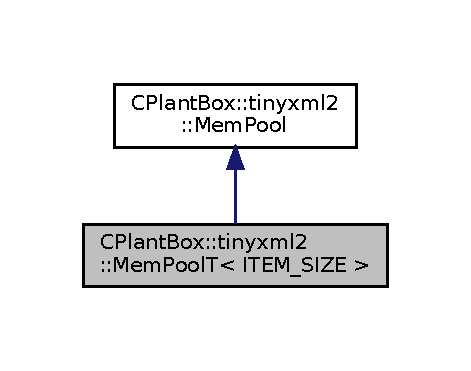
\includegraphics[width=226pt]{classCPlantBox_1_1tinyxml2_1_1MemPoolT__coll__graph}
\end{center}
\end{figure}
\subsection*{Public Types}
\begin{DoxyCompactItemize}
\item 
\mbox{\Hypertarget{classCPlantBox_1_1tinyxml2_1_1MemPoolT_ab57c95e6a7d77bf635b3f71ce8cfa758}\label{classCPlantBox_1_1tinyxml2_1_1MemPoolT_ab57c95e6a7d77bf635b3f71ce8cfa758}} 
enum \{ {\bfseries I\+T\+E\+M\+S\+\_\+\+P\+E\+R\+\_\+\+B\+L\+O\+CK} = (4 $\ast$ 1024) / I\+T\+E\+M\+\_\+\+S\+I\+ZE
 \}
\end{DoxyCompactItemize}
\subsection*{Public Member Functions}
\begin{DoxyCompactItemize}
\item 
\mbox{\Hypertarget{classCPlantBox_1_1tinyxml2_1_1MemPoolT_aa4963a0bf303983a95326a66982b9854}\label{classCPlantBox_1_1tinyxml2_1_1MemPoolT_aa4963a0bf303983a95326a66982b9854}} 
void {\bfseries Clear} ()
\item 
\mbox{\Hypertarget{classCPlantBox_1_1tinyxml2_1_1MemPoolT_aa6de67218da56d1648c12097acbbcd21}\label{classCPlantBox_1_1tinyxml2_1_1MemPoolT_aa6de67218da56d1648c12097acbbcd21}} 
virtual int {\bfseries Item\+Size} () const
\item 
\mbox{\Hypertarget{classCPlantBox_1_1tinyxml2_1_1MemPoolT_ab316e46d180846f7b5fef5a865ba6ea8}\label{classCPlantBox_1_1tinyxml2_1_1MemPoolT_ab316e46d180846f7b5fef5a865ba6ea8}} 
int {\bfseries Current\+Allocs} () const
\item 
\mbox{\Hypertarget{classCPlantBox_1_1tinyxml2_1_1MemPoolT_a5a31aade6ee5ba3bb107937f0f1bc0f7}\label{classCPlantBox_1_1tinyxml2_1_1MemPoolT_a5a31aade6ee5ba3bb107937f0f1bc0f7}} 
virtual void $\ast$ {\bfseries Alloc} ()
\item 
\mbox{\Hypertarget{classCPlantBox_1_1tinyxml2_1_1MemPoolT_aa0de3fa05ca21b89370a403c28d138e5}\label{classCPlantBox_1_1tinyxml2_1_1MemPoolT_aa0de3fa05ca21b89370a403c28d138e5}} 
virtual void {\bfseries Free} (void $\ast$mem)
\item 
\mbox{\Hypertarget{classCPlantBox_1_1tinyxml2_1_1MemPoolT_a42678b20a9a78d4b55e64f0359c2c2de}\label{classCPlantBox_1_1tinyxml2_1_1MemPoolT_a42678b20a9a78d4b55e64f0359c2c2de}} 
void {\bfseries Trace} (const char $\ast$name)
\item 
\mbox{\Hypertarget{classCPlantBox_1_1tinyxml2_1_1MemPoolT_aac5e75409ea5d555265684d05aa6222c}\label{classCPlantBox_1_1tinyxml2_1_1MemPoolT_aac5e75409ea5d555265684d05aa6222c}} 
void {\bfseries Set\+Tracked} ()
\item 
\mbox{\Hypertarget{classCPlantBox_1_1tinyxml2_1_1MemPoolT_aca9a6816d31994ae8d9cd704f90d14b8}\label{classCPlantBox_1_1tinyxml2_1_1MemPoolT_aca9a6816d31994ae8d9cd704f90d14b8}} 
int {\bfseries Untracked} () const
\end{DoxyCompactItemize}


The documentation for this class was generated from the following file\+:\begin{DoxyCompactItemize}
\item 
src/tinyxml2.\+h\end{DoxyCompactItemize}

\hypertarget{classCPlantBox_1_1Organ}{}\section{C\+Plant\+Box\+:\+:Organ Class Reference}
\label{classCPlantBox_1_1Organ}\index{C\+Plant\+Box\+::\+Organ@{C\+Plant\+Box\+::\+Organ}}


{\ttfamily \#include $<$Organ.\+h$>$}



Inheritance diagram for C\+Plant\+Box\+:\+:Organ\+:\nopagebreak
\begin{figure}[H]
\begin{center}
\leavevmode
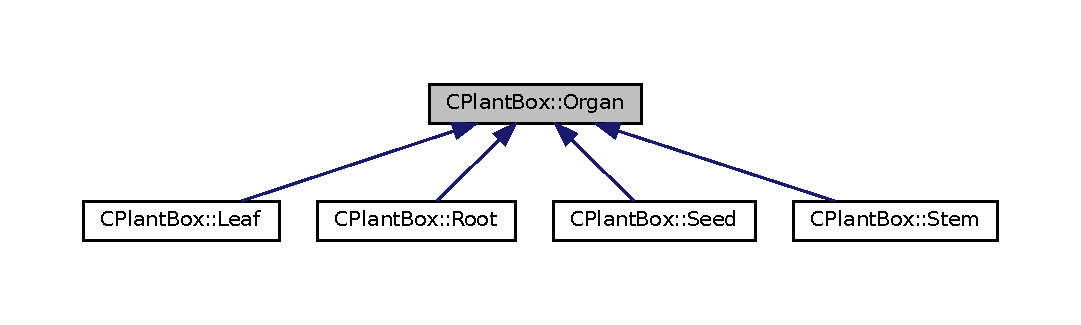
\includegraphics[width=350pt]{classCPlantBox_1_1Organ__inherit__graph}
\end{center}
\end{figure}


Collaboration diagram for C\+Plant\+Box\+:\+:Organ\+:\nopagebreak
\begin{figure}[H]
\begin{center}
\leavevmode
\includegraphics[width=350pt]{classCPlantBox_1_1Organ__coll__graph}
\end{center}
\end{figure}
\subsection*{Public Types}
\begin{DoxyCompactItemize}
\item 
\mbox{\Hypertarget{classCPlantBox_1_1Organ_a9161d0ffc2c515aa584d795367158482}\label{classCPlantBox_1_1Organ_a9161d0ffc2c515aa584d795367158482}} 
enum {\bfseries Organ\+Types} \{ \newline
{\bfseries ot\+\_\+seed} = 1, 
{\bfseries ot\+\_\+root} = 2, 
{\bfseries ot\+\_\+stem} = 4, 
{\bfseries ot\+\_\+leafe} = 8, 
\newline
{\bfseries ot\+\_\+shoot} = ot\+\_\+stem $\vert$ ot\+\_\+leafe, 
{\bfseries ot\+\_\+organ} = ot\+\_\+seed $\vert$ ot\+\_\+root $\vert$ ot\+\_\+stem $\vert$ ot\+\_\+leafe
 \}
\item 
\mbox{\Hypertarget{classCPlantBox_1_1Organ_ada94ab02398ad46f1f377c54459e81f2}\label{classCPlantBox_1_1Organ_ada94ab02398ad46f1f377c54459e81f2}} 
enum {\bfseries Tropism\+Types} \{ {\bfseries tt\+\_\+plagio} = 0, 
{\bfseries tt\+\_\+gravi} = 1, 
{\bfseries tt\+\_\+exo} = 2, 
{\bfseries tt\+\_\+hydro} = 3
 \}
\item 
\mbox{\Hypertarget{classCPlantBox_1_1Organ_a1e30e0dfd37b88380c06a1739e63b985}\label{classCPlantBox_1_1Organ_a1e30e0dfd37b88380c06a1739e63b985}} 
enum {\bfseries Growth\+Function\+Types} \{ {\bfseries gft\+\_\+negexp} = 1, 
{\bfseries gft\+\_\+linear} = 2
 \}
\item 
\mbox{\Hypertarget{classCPlantBox_1_1Organ_a72af68e2ca57d20c3a46a7d527f7e1e1}\label{classCPlantBox_1_1Organ_a72af68e2ca57d20c3a46a7d527f7e1e1}} 
enum {\bfseries Scalar\+Types} \{ \newline
{\bfseries st\+\_\+type} = 0, 
{\bfseries st\+\_\+radius} = 1, 
{\bfseries st\+\_\+order} = 2, 
{\bfseries st\+\_\+time} = 3, 
\newline
{\bfseries st\+\_\+length} = 4, 
{\bfseries st\+\_\+surface} = 5, 
{\bfseries st\+\_\+volume} = 6, 
{\bfseries st\+\_\+one} = 7, 
\newline
{\bfseries st\+\_\+userdata1} = 8, 
{\bfseries st\+\_\+userdata2} = 9, 
{\bfseries st\+\_\+userdata3} = 10, 
{\bfseries st\+\_\+parenttype} = 11, 
\newline
{\bfseries st\+\_\+lb} = 12, 
{\bfseries st\+\_\+la} = 13, 
{\bfseries st\+\_\+nob} = 14, 
{\bfseries st\+\_\+r} = 15, 
\newline
{\bfseries st\+\_\+theta} = 16, 
{\bfseries st\+\_\+rlt} = 17, 
{\bfseries st\+\_\+meanln} = 18, 
{\bfseries st\+\_\+sdln} = 19
 \}
\end{DoxyCompactItemize}
\subsection*{Public Member Functions}
\begin{DoxyCompactItemize}
\item 
\hyperlink{classCPlantBox_1_1Organ_a7cc5635a2b9a20facab79a78e7a4eb48}{Organ} (\hyperlink{classCPlantBox_1_1Plant}{Plant} $\ast$\hyperlink{classCPlantBox_1_1Organ_ac614456886ab270c6fd2617403e0f306}{plant}, \hyperlink{classCPlantBox_1_1Organ}{Organ} $\ast$\hyperlink{classCPlantBox_1_1Organ_a8ad90078d5ef859bd2ab71700854e286}{parent}, int subtype, double delay)
\item 
virtual \hyperlink{classCPlantBox_1_1Organ_a0c6757c6789c3508696ce3253f81aaa3}{$\sim$\+Organ} ()
\item 
\mbox{\Hypertarget{classCPlantBox_1_1Organ_abb608537d6c6d8888407eacdadca5518}\label{classCPlantBox_1_1Organ_abb608537d6c6d8888407eacdadca5518}} 
virtual int \hyperlink{classCPlantBox_1_1Organ_abb608537d6c6d8888407eacdadca5518}{organ\+Type} () const
\begin{DoxyCompactList}\small\item\em returns the organs type, overwrite for each organ \end{DoxyCompactList}\item 
\mbox{\Hypertarget{classCPlantBox_1_1Organ_a9046ebc480f02addf40388aebae7ecc1}\label{classCPlantBox_1_1Organ_a9046ebc480f02addf40388aebae7ecc1}} 
virtual \hyperlink{classCPlantBox_1_1Vector3d}{Vector3d} {\bfseries get\+Relative\+Origin} () const
\item 
\mbox{\Hypertarget{classCPlantBox_1_1Organ_a7c2299c7e83d9da1591d63bc5c7d2b17}\label{classCPlantBox_1_1Organ_a7c2299c7e83d9da1591d63bc5c7d2b17}} 
virtual void \hyperlink{classCPlantBox_1_1Organ_a7c2299c7e83d9da1591d63bc5c7d2b17}{set\+Relative\+Origin} (const \hyperlink{classCPlantBox_1_1Vector3d}{Vector3d} \&o)
\begin{DoxyCompactList}\small\item\em the relative position within the parent organ \end{DoxyCompactList}\item 
\mbox{\Hypertarget{classCPlantBox_1_1Organ_aa2a305a167faaca52f01f19eb894143f}\label{classCPlantBox_1_1Organ_aa2a305a167faaca52f01f19eb894143f}} 
virtual \hyperlink{classCPlantBox_1_1Matrix3d}{Matrix3d} \hyperlink{classCPlantBox_1_1Organ_aa2a305a167faaca52f01f19eb894143f}{get\+Relative\+Heading} () const
\begin{DoxyCompactList}\small\item\em the relative position within the parent organ \end{DoxyCompactList}\item 
\mbox{\Hypertarget{classCPlantBox_1_1Organ_a96ebcecf9a2acda92d3dd1d435ee64ff}\label{classCPlantBox_1_1Organ_a96ebcecf9a2acda92d3dd1d435ee64ff}} 
virtual void \hyperlink{classCPlantBox_1_1Organ_a96ebcecf9a2acda92d3dd1d435ee64ff}{set\+Relative\+Heading} (const \hyperlink{classCPlantBox_1_1Matrix3d}{Matrix3d} \&m)
\begin{DoxyCompactList}\small\item\em the heading in the parent organ \end{DoxyCompactList}\item 
\hyperlink{classCPlantBox_1_1Vector3d}{Vector3d} \hyperlink{classCPlantBox_1_1Organ_ac18526b4b44a40392a1f5db5ff2f6c72}{get\+Origin} () const
\begin{DoxyCompactList}\small\item\em the heading in the parent organ \end{DoxyCompactList}\item 
\hyperlink{classCPlantBox_1_1Matrix3d}{Matrix3d} \hyperlink{classCPlantBox_1_1Organ_a3436c97a754ba2b8633e0f47df3604d5}{get\+Heading} () const
\begin{DoxyCompactList}\small\item\em absolute heading of the organ \end{DoxyCompactList}\item 
\hyperlink{classCPlantBox_1_1Vector3d}{Vector3d} \hyperlink{classCPlantBox_1_1Organ_a17438f54d1d07af58867a4d257225e87}{get\+Node} (int i) const
\begin{DoxyCompactList}\small\item\em i-\/th node of the organ in absolute coordinates \end{DoxyCompactList}\item 
std\+::vector$<$ \hyperlink{classCPlantBox_1_1Vector3d}{Vector3d} $>$ \hyperlink{classCPlantBox_1_1Organ_af990e5df473327cb2cdb6293d5117419}{get\+Nodes} () const
\item 
\hyperlink{classCPlantBox_1_1OrganRandomOrganParameter}{Organ\+Random\+Organ\+Parameter} $\ast$ \hyperlink{classCPlantBox_1_1Organ_aa6668fc995d856d1a06c92af06155f00}{get\+Organ\+Random\+Organ\+Parameter} () const
\begin{DoxyCompactList}\small\item\em converts all relative nodes to absolute coordinates \end{DoxyCompactList}\item 
virtual void \hyperlink{classCPlantBox_1_1Organ_acf519fc6730c0adbb2a82b7702ff7a28}{simulate} (double dt, bool silence=false)
\begin{DoxyCompactList}\small\item\em growth for a time span of \end{DoxyCompactList}\item 
std\+::vector$<$ \hyperlink{classCPlantBox_1_1Organ}{Organ} $\ast$ $>$ \hyperlink{classCPlantBox_1_1Organ_aee7e856229fd2ac996c0033aacead4c1}{get\+Organs} (unsigned int otype)
\begin{DoxyCompactList}\small\item\em the organ including successors in a sequential vector \end{DoxyCompactList}\item 
void \hyperlink{classCPlantBox_1_1Organ_a96e286dd479eca6b338630225939c636}{get\+Organs} (unsigned int otype, std\+::vector$<$ \hyperlink{classCPlantBox_1_1Organ}{Organ} $\ast$$>$ \&v)
\begin{DoxyCompactList}\small\item\em the organ including successors in a sequential vector \end{DoxyCompactList}\item 
virtual double \hyperlink{classCPlantBox_1_1Organ_adf7d115c625341e0f6d291c750b05e5c}{get\+Scalar} (std\+::string name) const
\begin{DoxyCompactList}\small\item\em returns an organ parameter of Plant\+::\+Scalar\+Type \end{DoxyCompactList}\item 
virtual std\+::string \hyperlink{classCPlantBox_1_1Organ_a9f823aebd19519096e899e65604f239f}{to\+String} () const
\item 
virtual void \hyperlink{classCPlantBox_1_1Organ_acdad546c90e915b61ac3606f1f841ba1}{write\+R\+S\+ML} (std\+::ostream \&cout, std\+::string indent) const
\begin{DoxyCompactList}\small\item\em writes a R\+S\+ML root tag \end{DoxyCompactList}\item 
\mbox{\Hypertarget{classCPlantBox_1_1Organ_aa13c0f14d524c6fde4ee768b086f558f}\label{classCPlantBox_1_1Organ_aa13c0f14d524c6fde4ee768b086f558f}} 
size\+\_\+t \hyperlink{classCPlantBox_1_1Organ_aa13c0f14d524c6fde4ee768b086f558f}{get\+Number\+Of\+Nodes} () const
\begin{DoxyCompactList}\small\item\em number of nodes of the organ \end{DoxyCompactList}\item 
\mbox{\Hypertarget{classCPlantBox_1_1Organ_a8de3325c509c106596dacf095f00b67f}\label{classCPlantBox_1_1Organ_a8de3325c509c106596dacf095f00b67f}} 
int \hyperlink{classCPlantBox_1_1Organ_a8de3325c509c106596dacf095f00b67f}{get\+Node\+ID} (int i) const
\begin{DoxyCompactList}\small\item\em unique identifier of i-\/th node \end{DoxyCompactList}\item 
\mbox{\Hypertarget{classCPlantBox_1_1Organ_a84501e4b05c160ea826ee673889605da}\label{classCPlantBox_1_1Organ_a84501e4b05c160ea826ee673889605da}} 
double \hyperlink{classCPlantBox_1_1Organ_a84501e4b05c160ea826ee673889605da}{get\+Node\+CT} (int i) const
\begin{DoxyCompactList}\small\item\em creation time of i-\/th node \end{DoxyCompactList}\item 
\mbox{\Hypertarget{classCPlantBox_1_1Organ_a27f2f56687057a06300739bf877a92d9}\label{classCPlantBox_1_1Organ_a27f2f56687057a06300739bf877a92d9}} 
std\+::vector$<$ \hyperlink{classCPlantBox_1_1Organ}{Organ} $\ast$ $>$ {\bfseries get\+Children} (unsigned int otype)
\end{DoxyCompactItemize}
\subsection*{Public Attributes}
\begin{DoxyCompactItemize}
\item 
\mbox{\Hypertarget{classCPlantBox_1_1Organ_ac614456886ab270c6fd2617403e0f306}\label{classCPlantBox_1_1Organ_ac614456886ab270c6fd2617403e0f306}} 
\hyperlink{classCPlantBox_1_1Plant}{Plant} $\ast$ \hyperlink{classCPlantBox_1_1Organ_ac614456886ab270c6fd2617403e0f306}{plant}
\begin{DoxyCompactList}\small\item\em the plant of which this organ is part of \end{DoxyCompactList}\item 
\mbox{\Hypertarget{classCPlantBox_1_1Organ_a8ad90078d5ef859bd2ab71700854e286}\label{classCPlantBox_1_1Organ_a8ad90078d5ef859bd2ab71700854e286}} 
\hyperlink{classCPlantBox_1_1Organ}{Organ} $\ast$ \hyperlink{classCPlantBox_1_1Organ_a8ad90078d5ef859bd2ab71700854e286}{parent}
\begin{DoxyCompactList}\small\item\em pointer to the parent organ (equals nullptr if it has no parent) \end{DoxyCompactList}\item 
\mbox{\Hypertarget{classCPlantBox_1_1Organ_ab664ce01c2d6a2f4090408b8b1d438dd}\label{classCPlantBox_1_1Organ_ab664ce01c2d6a2f4090408b8b1d438dd}} 
std\+::vector$<$ \hyperlink{classCPlantBox_1_1Organ}{Organ} $\ast$ $>$ \hyperlink{classCPlantBox_1_1Organ_ab664ce01c2d6a2f4090408b8b1d438dd}{children}
\begin{DoxyCompactList}\small\item\em the successive organs \end{DoxyCompactList}\item 
\mbox{\Hypertarget{classCPlantBox_1_1Organ_a4c567a27db0b5e4262067f4cbbf59553}\label{classCPlantBox_1_1Organ_a4c567a27db0b5e4262067f4cbbf59553}} 
int \hyperlink{classCPlantBox_1_1Organ_a4c567a27db0b5e4262067f4cbbf59553}{id}
\begin{DoxyCompactList}\small\item\em unique organ id, (not used so far) \end{DoxyCompactList}\item 
\mbox{\Hypertarget{classCPlantBox_1_1Organ_a59ba6de6ced8b8d7b20788bd7656cee2}\label{classCPlantBox_1_1Organ_a59ba6de6ced8b8d7b20788bd7656cee2}} 
\hyperlink{classCPlantBox_1_1SpecificOrganParamter}{Specific\+Organ\+Paramter} $\ast$ \hyperlink{classCPlantBox_1_1Organ_a59ba6de6ced8b8d7b20788bd7656cee2}{param} = nullptr
\begin{DoxyCompactList}\small\item\em the parameters of this root \end{DoxyCompactList}\item 
\mbox{\Hypertarget{classCPlantBox_1_1Organ_a0889e6bf6d670b945de355dbc6e96965}\label{classCPlantBox_1_1Organ_a0889e6bf6d670b945de355dbc6e96965}} 
bool \hyperlink{classCPlantBox_1_1Organ_a0889e6bf6d670b945de355dbc6e96965}{alive} = 1
\begin{DoxyCompactList}\small\item\em true\+: alive, false\+: dead \end{DoxyCompactList}\item 
\mbox{\Hypertarget{classCPlantBox_1_1Organ_a37cba2abb3c4052d7e69b57019589b78}\label{classCPlantBox_1_1Organ_a37cba2abb3c4052d7e69b57019589b78}} 
bool \hyperlink{classCPlantBox_1_1Organ_a37cba2abb3c4052d7e69b57019589b78}{active} = 1
\begin{DoxyCompactList}\small\item\em true\+: active, false\+: root stopped growing \end{DoxyCompactList}\item 
\mbox{\Hypertarget{classCPlantBox_1_1Organ_a4f17f0bfe7f03eedf4138fd8fe51376d}\label{classCPlantBox_1_1Organ_a4f17f0bfe7f03eedf4138fd8fe51376d}} 
double \hyperlink{classCPlantBox_1_1Organ_a4f17f0bfe7f03eedf4138fd8fe51376d}{age} = 0
\begin{DoxyCompactList}\small\item\em current age \mbox{[}days\mbox{]} \end{DoxyCompactList}\item 
\mbox{\Hypertarget{classCPlantBox_1_1Organ_a94f5b16aa7ebc3912501051281fe88dc}\label{classCPlantBox_1_1Organ_a94f5b16aa7ebc3912501051281fe88dc}} 
double \hyperlink{classCPlantBox_1_1Organ_a94f5b16aa7ebc3912501051281fe88dc}{length} = 0
\begin{DoxyCompactList}\small\item\em actual length \mbox{[}cm\mbox{]} of the root. might differ from get\+Length(age) in case of impeded root growth \end{DoxyCompactList}\item 
\mbox{\Hypertarget{classCPlantBox_1_1Organ_a3c27ae9dcbe4f4f8a0f07450d8c4ac14}\label{classCPlantBox_1_1Organ_a3c27ae9dcbe4f4f8a0f07450d8c4ac14}} 
std\+::vector$<$ \hyperlink{classCPlantBox_1_1Vector3d}{Vector3d} $>$ \hyperlink{classCPlantBox_1_1Organ_a3c27ae9dcbe4f4f8a0f07450d8c4ac14}{r\+\_\+nodes}
\begin{DoxyCompactList}\small\item\em relative nodes of the root \end{DoxyCompactList}\item 
\mbox{\Hypertarget{classCPlantBox_1_1Organ_ab9e80fa3f95812af2ee720719f8457df}\label{classCPlantBox_1_1Organ_ab9e80fa3f95812af2ee720719f8457df}} 
std\+::vector$<$ int $>$ \hyperlink{classCPlantBox_1_1Organ_ab9e80fa3f95812af2ee720719f8457df}{node\+I\+Ds}
\begin{DoxyCompactList}\small\item\em unique node identifier \end{DoxyCompactList}\item 
\mbox{\Hypertarget{classCPlantBox_1_1Organ_a2fad84a9d24de4c66d706510a9c50d09}\label{classCPlantBox_1_1Organ_a2fad84a9d24de4c66d706510a9c50d09}} 
std\+::vector$<$ double $>$ \hyperlink{classCPlantBox_1_1Organ_a2fad84a9d24de4c66d706510a9c50d09}{nctimes}
\begin{DoxyCompactList}\small\item\em node creation times \mbox{[}days\mbox{]} \end{DoxyCompactList}\end{DoxyCompactItemize}
\subsection*{Static Public Attributes}
\begin{DoxyCompactItemize}
\item 
\mbox{\Hypertarget{classCPlantBox_1_1Organ_a6df035488e363a748e220eb766c0776d}\label{classCPlantBox_1_1Organ_a6df035488e363a748e220eb766c0776d}} 
static const std\+::vector$<$ std\+::string $>$ \hyperlink{classCPlantBox_1_1Organ_a6df035488e363a748e220eb766c0776d}{scalar\+Type\+Names}
\begin{DoxyCompactList}\small\item\em the corresponding names \end{DoxyCompactList}\end{DoxyCompactItemize}


\subsection{Detailed Description}
\hyperlink{classCPlantBox_1_1Organ}{Organ}

Base class of seed, root, shoot and leaf 

\subsection{Constructor \& Destructor Documentation}
\mbox{\Hypertarget{classCPlantBox_1_1Organ_a7cc5635a2b9a20facab79a78e7a4eb48}\label{classCPlantBox_1_1Organ_a7cc5635a2b9a20facab79a78e7a4eb48}} 
\index{C\+Plant\+Box\+::\+Organ@{C\+Plant\+Box\+::\+Organ}!Organ@{Organ}}
\index{Organ@{Organ}!C\+Plant\+Box\+::\+Organ@{C\+Plant\+Box\+::\+Organ}}
\subsubsection{\texorpdfstring{Organ()}{Organ()}}
{\footnotesize\ttfamily C\+Plant\+Box\+::\+Organ\+::\+Organ (\begin{DoxyParamCaption}\item[{\hyperlink{classCPlantBox_1_1Plant}{Plant} $\ast$}]{plant,  }\item[{\hyperlink{classCPlantBox_1_1Organ}{Organ} $\ast$}]{parent,  }\item[{int}]{subtype,  }\item[{double}]{delay }\end{DoxyParamCaption})}

Constructor \mbox{\Hypertarget{classCPlantBox_1_1Organ_a0c6757c6789c3508696ce3253f81aaa3}\label{classCPlantBox_1_1Organ_a0c6757c6789c3508696ce3253f81aaa3}} 
\index{C\+Plant\+Box\+::\+Organ@{C\+Plant\+Box\+::\+Organ}!````~Organ@{$\sim$\+Organ}}
\index{````~Organ@{$\sim$\+Organ}!C\+Plant\+Box\+::\+Organ@{C\+Plant\+Box\+::\+Organ}}
\subsubsection{\texorpdfstring{$\sim$\+Organ()}{~Organ()}}
{\footnotesize\ttfamily C\+Plant\+Box\+::\+Organ\+::$\sim$\+Organ (\begin{DoxyParamCaption}{ }\end{DoxyParamCaption})\hspace{0.3cm}{\ttfamily [virtual]}}

Destructor, tell the kids (bad news) 

\subsection{Member Function Documentation}
\mbox{\Hypertarget{classCPlantBox_1_1Organ_a3436c97a754ba2b8633e0f47df3604d5}\label{classCPlantBox_1_1Organ_a3436c97a754ba2b8633e0f47df3604d5}} 
\index{C\+Plant\+Box\+::\+Organ@{C\+Plant\+Box\+::\+Organ}!get\+Heading@{get\+Heading}}
\index{get\+Heading@{get\+Heading}!C\+Plant\+Box\+::\+Organ@{C\+Plant\+Box\+::\+Organ}}
\subsubsection{\texorpdfstring{get\+Heading()}{getHeading()}}
{\footnotesize\ttfamily \hyperlink{classCPlantBox_1_1Matrix3d}{Matrix3d} C\+Plant\+Box\+::\+Organ\+::get\+Heading (\begin{DoxyParamCaption}{ }\end{DoxyParamCaption}) const}



absolute heading of the organ 

Absolute organ heading Hn =(A0$\ast$\+A1$\ast$..An), where H is the absolute Heading, and A are the relative headings \mbox{\Hypertarget{classCPlantBox_1_1Organ_a17438f54d1d07af58867a4d257225e87}\label{classCPlantBox_1_1Organ_a17438f54d1d07af58867a4d257225e87}} 
\index{C\+Plant\+Box\+::\+Organ@{C\+Plant\+Box\+::\+Organ}!get\+Node@{get\+Node}}
\index{get\+Node@{get\+Node}!C\+Plant\+Box\+::\+Organ@{C\+Plant\+Box\+::\+Organ}}
\subsubsection{\texorpdfstring{get\+Node()}{getNode()}}
{\footnotesize\ttfamily \hyperlink{classCPlantBox_1_1Vector3d}{Vector3d} C\+Plant\+Box\+::\+Organ\+::get\+Node (\begin{DoxyParamCaption}\item[{int}]{i }\end{DoxyParamCaption}) const}



i-\/th node of the organ in absolute coordinates 

Computes the absolute node coordinate (A$\ast$x+o) \mbox{\Hypertarget{classCPlantBox_1_1Organ_af990e5df473327cb2cdb6293d5117419}\label{classCPlantBox_1_1Organ_af990e5df473327cb2cdb6293d5117419}} 
\index{C\+Plant\+Box\+::\+Organ@{C\+Plant\+Box\+::\+Organ}!get\+Nodes@{get\+Nodes}}
\index{get\+Nodes@{get\+Nodes}!C\+Plant\+Box\+::\+Organ@{C\+Plant\+Box\+::\+Organ}}
\subsubsection{\texorpdfstring{get\+Nodes()}{getNodes()}}
{\footnotesize\ttfamily std\+::vector$<$ \hyperlink{classCPlantBox_1_1Vector3d}{Vector3d} $>$ C\+Plant\+Box\+::\+Organ\+::get\+Nodes (\begin{DoxyParamCaption}{ }\end{DoxyParamCaption}) const}

Computes the absolute node coordinates for all relative coordinates (A$\ast$x\+\_\+i+o) \mbox{\Hypertarget{classCPlantBox_1_1Organ_aa6668fc995d856d1a06c92af06155f00}\label{classCPlantBox_1_1Organ_aa6668fc995d856d1a06c92af06155f00}} 
\index{C\+Plant\+Box\+::\+Organ@{C\+Plant\+Box\+::\+Organ}!get\+Organ\+Random\+Organ\+Parameter@{get\+Organ\+Random\+Organ\+Parameter}}
\index{get\+Organ\+Random\+Organ\+Parameter@{get\+Organ\+Random\+Organ\+Parameter}!C\+Plant\+Box\+::\+Organ@{C\+Plant\+Box\+::\+Organ}}
\subsubsection{\texorpdfstring{get\+Organ\+Random\+Organ\+Parameter()}{getOrganRandomOrganParameter()}}
{\footnotesize\ttfamily \hyperlink{classCPlantBox_1_1OrganRandomOrganParameter}{Organ\+Random\+Organ\+Parameter} $\ast$ C\+Plant\+Box\+::\+Organ\+::get\+Organ\+Random\+Organ\+Parameter (\begin{DoxyParamCaption}{ }\end{DoxyParamCaption}) const}



converts all relative nodes to absolute coordinates 

organ type parameter

Asks the plant for the organ type parameter \mbox{\Hypertarget{classCPlantBox_1_1Organ_aee7e856229fd2ac996c0033aacead4c1}\label{classCPlantBox_1_1Organ_aee7e856229fd2ac996c0033aacead4c1}} 
\index{C\+Plant\+Box\+::\+Organ@{C\+Plant\+Box\+::\+Organ}!get\+Organs@{get\+Organs}}
\index{get\+Organs@{get\+Organs}!C\+Plant\+Box\+::\+Organ@{C\+Plant\+Box\+::\+Organ}}
\subsubsection{\texorpdfstring{get\+Organs()}{getOrgans()}\hspace{0.1cm}{\footnotesize\ttfamily [1/2]}}
{\footnotesize\ttfamily std\+::vector$<$ \hyperlink{classCPlantBox_1_1Organ}{Organ} $\ast$ $>$ C\+Plant\+Box\+::\+Organ\+::get\+Organs (\begin{DoxyParamCaption}\item[{unsigned int}]{otype }\end{DoxyParamCaption})}



the organ including successors in a sequential vector 

Returns the organs as sequential list, copies only organs with more than 1 node.

\begin{DoxyReturn}{Returns}
sequential list of organs 
\end{DoxyReturn}
\mbox{\Hypertarget{classCPlantBox_1_1Organ_a96e286dd479eca6b338630225939c636}\label{classCPlantBox_1_1Organ_a96e286dd479eca6b338630225939c636}} 
\index{C\+Plant\+Box\+::\+Organ@{C\+Plant\+Box\+::\+Organ}!get\+Organs@{get\+Organs}}
\index{get\+Organs@{get\+Organs}!C\+Plant\+Box\+::\+Organ@{C\+Plant\+Box\+::\+Organ}}
\subsubsection{\texorpdfstring{get\+Organs()}{getOrgans()}\hspace{0.1cm}{\footnotesize\ttfamily [2/2]}}
{\footnotesize\ttfamily void C\+Plant\+Box\+::\+Organ\+::get\+Organs (\begin{DoxyParamCaption}\item[{unsigned int}]{otype,  }\item[{std\+::vector$<$ \hyperlink{classCPlantBox_1_1Organ}{Organ} $\ast$$>$ \&}]{v }\end{DoxyParamCaption})}



the organ including successors in a sequential vector 

Returns the organs as sequential list, copies only organs with more than 1 node.


\begin{DoxyParams}{Parameters}
{\em v} & adds the organ sub tree to this vector \\
\hline
\end{DoxyParams}
\mbox{\Hypertarget{classCPlantBox_1_1Organ_ac18526b4b44a40392a1f5db5ff2f6c72}\label{classCPlantBox_1_1Organ_ac18526b4b44a40392a1f5db5ff2f6c72}} 
\index{C\+Plant\+Box\+::\+Organ@{C\+Plant\+Box\+::\+Organ}!get\+Origin@{get\+Origin}}
\index{get\+Origin@{get\+Origin}!C\+Plant\+Box\+::\+Organ@{C\+Plant\+Box\+::\+Organ}}
\subsubsection{\texorpdfstring{get\+Origin()}{getOrigin()}}
{\footnotesize\ttfamily \hyperlink{classCPlantBox_1_1Vector3d}{Vector3d} C\+Plant\+Box\+::\+Organ\+::get\+Origin (\begin{DoxyParamCaption}{ }\end{DoxyParamCaption}) const}



the heading in the parent organ 

absolute coordinates of the organ origin

The organ origin in absolute coordinates p\+\_\+abs = A0(p1+\+A1(p2+\+A2(p3+... A(n-\/1)(pn ) )))), where A are the relative headings, p are the relative origins \mbox{\Hypertarget{classCPlantBox_1_1Organ_adf7d115c625341e0f6d291c750b05e5c}\label{classCPlantBox_1_1Organ_adf7d115c625341e0f6d291c750b05e5c}} 
\index{C\+Plant\+Box\+::\+Organ@{C\+Plant\+Box\+::\+Organ}!get\+Scalar@{get\+Scalar}}
\index{get\+Scalar@{get\+Scalar}!C\+Plant\+Box\+::\+Organ@{C\+Plant\+Box\+::\+Organ}}
\subsubsection{\texorpdfstring{get\+Scalar()}{getScalar()}}
{\footnotesize\ttfamily double C\+Plant\+Box\+::\+Organ\+::get\+Scalar (\begin{DoxyParamCaption}\item[{std\+::string}]{name }\end{DoxyParamCaption}) const\hspace{0.3cm}{\ttfamily [virtual]}}



returns an organ parameter of Plant\+::\+Scalar\+Type 

Returns the parameter called 
\begin{DoxyParams}{Parameters}
{\em name} & \\
\hline
\end{DoxyParams}


Reimplemented in \hyperlink{classCPlantBox_1_1Root_a23fac3d7c3b15e5f270d76b56c693ab9}{C\+Plant\+Box\+::\+Root}, \hyperlink{classCPlantBox_1_1Stem_ace47428771936118b0775ca9d23e5f4f}{C\+Plant\+Box\+::\+Stem}, and \hyperlink{classCPlantBox_1_1Leaf_a97bb6cc92a59f0d137eb6b497b5d376e}{C\+Plant\+Box\+::\+Leaf}.

\mbox{\Hypertarget{classCPlantBox_1_1Organ_acf519fc6730c0adbb2a82b7702ff7a28}\label{classCPlantBox_1_1Organ_acf519fc6730c0adbb2a82b7702ff7a28}} 
\index{C\+Plant\+Box\+::\+Organ@{C\+Plant\+Box\+::\+Organ}!simulate@{simulate}}
\index{simulate@{simulate}!C\+Plant\+Box\+::\+Organ@{C\+Plant\+Box\+::\+Organ}}
\subsubsection{\texorpdfstring{simulate()}{simulate()}}
{\footnotesize\ttfamily void C\+Plant\+Box\+::\+Organ\+::simulate (\begin{DoxyParamCaption}\item[{double}]{dt,  }\item[{bool}]{silence = {\ttfamily false} }\end{DoxyParamCaption})\hspace{0.3cm}{\ttfamily [virtual]}}



growth for a time span of 


\begin{DoxyParams}{Parameters}
{\em dt} & \\
\hline
\end{DoxyParams}
Calls suborgans (children) 

Reimplemented in \hyperlink{classCPlantBox_1_1Root_af2fa9d229ab05897214e0ec224f0ae71}{C\+Plant\+Box\+::\+Root}, \hyperlink{classCPlantBox_1_1Stem_ad2f7f8607fe02dbe2f4d4335248cf90b}{C\+Plant\+Box\+::\+Stem}, and \hyperlink{classCPlantBox_1_1Leaf_ac8f35a92020107f44059b995e44af5d6}{C\+Plant\+Box\+::\+Leaf}.

\mbox{\Hypertarget{classCPlantBox_1_1Organ_a9f823aebd19519096e899e65604f239f}\label{classCPlantBox_1_1Organ_a9f823aebd19519096e899e65604f239f}} 
\index{C\+Plant\+Box\+::\+Organ@{C\+Plant\+Box\+::\+Organ}!to\+String@{to\+String}}
\index{to\+String@{to\+String}!C\+Plant\+Box\+::\+Organ@{C\+Plant\+Box\+::\+Organ}}
\subsubsection{\texorpdfstring{to\+String()}{toString()}}
{\footnotesize\ttfamily std\+::string C\+Plant\+Box\+::\+Organ\+::to\+String (\begin{DoxyParamCaption}{ }\end{DoxyParamCaption}) const\hspace{0.3cm}{\ttfamily [virtual]}}

Quick info about the object for debugging T\+O\+DO change param to param or param 

Reimplemented in \hyperlink{classCPlantBox_1_1Root_a389312a40582e21c1eaa6c5ebb927f2e}{C\+Plant\+Box\+::\+Root}, \hyperlink{classCPlantBox_1_1Leaf_a7c09270825fa8f874dcf409969dbb554}{C\+Plant\+Box\+::\+Leaf}, \hyperlink{classCPlantBox_1_1Stem_a08ed9dc10ef3ea13c90bc326e6cc989b}{C\+Plant\+Box\+::\+Stem}, and \hyperlink{classCPlantBox_1_1Seed_a83a1493777594b1e92d31d6d3db4258b}{C\+Plant\+Box\+::\+Seed}.

\mbox{\Hypertarget{classCPlantBox_1_1Organ_acdad546c90e915b61ac3606f1f841ba1}\label{classCPlantBox_1_1Organ_acdad546c90e915b61ac3606f1f841ba1}} 
\index{C\+Plant\+Box\+::\+Organ@{C\+Plant\+Box\+::\+Organ}!write\+R\+S\+ML@{write\+R\+S\+ML}}
\index{write\+R\+S\+ML@{write\+R\+S\+ML}!C\+Plant\+Box\+::\+Organ@{C\+Plant\+Box\+::\+Organ}}
\subsubsection{\texorpdfstring{write\+R\+S\+M\+L()}{writeRSML()}}
{\footnotesize\ttfamily void C\+Plant\+Box\+::\+Organ\+::write\+R\+S\+ML (\begin{DoxyParamCaption}\item[{std\+::ostream \&}]{cout,  }\item[{std\+::string}]{indent }\end{DoxyParamCaption}) const\hspace{0.3cm}{\ttfamily [virtual]}}



writes a R\+S\+ML root tag 

writes R\+S\+ML root tag (todo update for general organs)


\begin{DoxyParams}{Parameters}
{\em cout} & typically a file out stream \\
\hline
{\em indent} & we care for looks \\
\hline
\end{DoxyParams}


Reimplemented in \hyperlink{classCPlantBox_1_1Root_accf492ad0fa522fccc43588d1cde4610}{C\+Plant\+Box\+::\+Root}, \hyperlink{classCPlantBox_1_1Leaf_a0b5fbb524de825790da55551a212d4a0}{C\+Plant\+Box\+::\+Leaf}, and \hyperlink{classCPlantBox_1_1Stem_ae4087e7edf3b51619d6e8fd03a3c9ec8}{C\+Plant\+Box\+::\+Stem}.



The documentation for this class was generated from the following files\+:\begin{DoxyCompactItemize}
\item 
src/Organ.\+h\item 
src/Organ.\+cpp\end{DoxyCompactItemize}

\hypertarget{classCPlantBox_1_1OrganRandomOrganParameter}{}\section{C\+Plant\+Box\+:\+:Organ\+Random\+Organ\+Parameter Class Reference}
\label{classCPlantBox_1_1OrganRandomOrganParameter}\index{C\+Plant\+Box\+::\+Organ\+Random\+Organ\+Parameter@{C\+Plant\+Box\+::\+Organ\+Random\+Organ\+Parameter}}


{\ttfamily \#include $<$Model\+Parameter.\+h$>$}



Inheritance diagram for C\+Plant\+Box\+:\+:Organ\+Random\+Organ\+Parameter\+:\nopagebreak
\begin{figure}[H]
\begin{center}
\leavevmode
\includegraphics[width=350pt]{classCPlantBox_1_1OrganRandomOrganParameter__inherit__graph}
\end{center}
\end{figure}
\subsection*{Public Member Functions}
\begin{DoxyCompactItemize}
\item 
\mbox{\Hypertarget{classCPlantBox_1_1OrganRandomOrganParameter_a62915589b7b8e08c70c77c6402b026d1}\label{classCPlantBox_1_1OrganRandomOrganParameter_a62915589b7b8e08c70c77c6402b026d1}} 
virtual \hyperlink{classCPlantBox_1_1SpecificOrganParamter}{Specific\+Organ\+Paramter} $\ast$ {\bfseries realize} () const
\item 
\mbox{\Hypertarget{classCPlantBox_1_1OrganRandomOrganParameter_a564a3f0e973eb82b55ff0cef392eb077}\label{classCPlantBox_1_1OrganRandomOrganParameter_a564a3f0e973eb82b55ff0cef392eb077}} 
virtual void {\bfseries read\+X\+ML} (const \hyperlink{classCPlantBox_1_1tinyxml2_1_1XMLElement}{tinyxml2\+::\+X\+M\+L\+Element} $\ast$ele)
\item 
\mbox{\Hypertarget{classCPlantBox_1_1OrganRandomOrganParameter_aaab3491ac35f75fa9a25bf05104e0b0f}\label{classCPlantBox_1_1OrganRandomOrganParameter_aaab3491ac35f75fa9a25bf05104e0b0f}} 
virtual std\+::string {\bfseries write\+X\+ML} (F\+I\+LE $\ast$fp) const
\item 
\mbox{\Hypertarget{classCPlantBox_1_1OrganRandomOrganParameter_adbf24f95c8bbd94714c1000697ec4001}\label{classCPlantBox_1_1OrganRandomOrganParameter_adbf24f95c8bbd94714c1000697ec4001}} 
virtual std\+::string {\bfseries to\+String} () const
\item 
\mbox{\Hypertarget{classCPlantBox_1_1OrganRandomOrganParameter_a4eba421bf3955954392260ff256da5a0}\label{classCPlantBox_1_1OrganRandomOrganParameter_a4eba421bf3955954392260ff256da5a0}} 
void {\bfseries get\+Attribute} (const \hyperlink{classCPlantBox_1_1tinyxml2_1_1XMLElement}{tinyxml2\+::\+X\+M\+L\+Element} $\ast$ele2, const char $\ast$attr\+\_\+name, const char $\ast$para\+\_\+name, double \&attr, double \&deviation)
\item 
\mbox{\Hypertarget{classCPlantBox_1_1OrganRandomOrganParameter_aabc58cf8d0d3e3c03b29246b83588d1f}\label{classCPlantBox_1_1OrganRandomOrganParameter_aabc58cf8d0d3e3c03b29246b83588d1f}} 
void {\bfseries get\+Attribute} (const \hyperlink{classCPlantBox_1_1tinyxml2_1_1XMLElement}{tinyxml2\+::\+X\+M\+L\+Element} $\ast$ele2, const char $\ast$attr\+\_\+name, const char $\ast$para\+\_\+name, int \&attr, double \&deviation)
\item 
\mbox{\Hypertarget{classCPlantBox_1_1OrganRandomOrganParameter_a728a2f0248a1033ca741dfd7905771b9}\label{classCPlantBox_1_1OrganRandomOrganParameter_a728a2f0248a1033ca741dfd7905771b9}} 
void {\bfseries get\+Attribute} (const \hyperlink{classCPlantBox_1_1tinyxml2_1_1XMLElement}{tinyxml2\+::\+X\+M\+L\+Element} $\ast$ele2, const char $\ast$attr\+\_\+name, const char $\ast$para\+\_\+name, double \&attr, double \&deviation, int \&functiontype)
\item 
\mbox{\Hypertarget{classCPlantBox_1_1OrganRandomOrganParameter_aa0d2c68d49367b4389942b55c3518afd}\label{classCPlantBox_1_1OrganRandomOrganParameter_aa0d2c68d49367b4389942b55c3518afd}} 
void {\bfseries get\+Attribute} (const \hyperlink{classCPlantBox_1_1tinyxml2_1_1XMLElement}{tinyxml2\+::\+X\+M\+L\+Element} $\ast$ele2, const char $\ast$attr\+\_\+name, const char $\ast$para\+\_\+name, std\+::vector$<$ int $>$ \&successor, std\+::vector$<$ double $>$ \&successorP)
\item 
\mbox{\Hypertarget{classCPlantBox_1_1OrganRandomOrganParameter_aa34c93906eecb2fc67457720cb52d334}\label{classCPlantBox_1_1OrganRandomOrganParameter_aa34c93906eecb2fc67457720cb52d334}} 
void {\bfseries get\+Attribute} (const \hyperlink{classCPlantBox_1_1tinyxml2_1_1XMLElement}{tinyxml2\+::\+X\+M\+L\+Element} $\ast$ele2, const char $\ast$attr\+\_\+name, const char $\ast$para\+\_\+name, double \&attr)
\item 
\mbox{\Hypertarget{classCPlantBox_1_1OrganRandomOrganParameter_aabfc0756cab376654621f8f49542c4f3}\label{classCPlantBox_1_1OrganRandomOrganParameter_aabfc0756cab376654621f8f49542c4f3}} 
void {\bfseries get\+Attribute} (const \hyperlink{classCPlantBox_1_1tinyxml2_1_1XMLElement}{tinyxml2\+::\+X\+M\+L\+Element} $\ast$ele2, const char $\ast$attr\+\_\+name, const char $\ast$para\+\_\+name, int \&attr)
\item 
\mbox{\Hypertarget{classCPlantBox_1_1OrganRandomOrganParameter_a45f507c8e6bad457984a2e52c157e00b}\label{classCPlantBox_1_1OrganRandomOrganParameter_a45f507c8e6bad457984a2e52c157e00b}} 
void \hyperlink{classCPlantBox_1_1OrganRandomOrganParameter_a45f507c8e6bad457984a2e52c157e00b}{set\+Seed} (double seed) const
\begin{DoxyCompactList}\small\item\em Sets the seed of the random number generator. \end{DoxyCompactList}\item 
\mbox{\Hypertarget{classCPlantBox_1_1OrganRandomOrganParameter_a786d284ce6233ac93b1ea878ed048024}\label{classCPlantBox_1_1OrganRandomOrganParameter_a786d284ce6233ac93b1ea878ed048024}} 
double \hyperlink{classCPlantBox_1_1OrganRandomOrganParameter_a786d284ce6233ac93b1ea878ed048024}{rand} () const
\begin{DoxyCompactList}\small\item\em Uniformly distributed random number (0,1) \end{DoxyCompactList}\item 
\mbox{\Hypertarget{classCPlantBox_1_1OrganRandomOrganParameter_aad4819a51429f41944b8649b6bf8c425}\label{classCPlantBox_1_1OrganRandomOrganParameter_aad4819a51429f41944b8649b6bf8c425}} 
double \hyperlink{classCPlantBox_1_1OrganRandomOrganParameter_aad4819a51429f41944b8649b6bf8c425}{randn} () const
\begin{DoxyCompactList}\small\item\em Normally distributed random number (0,1) \end{DoxyCompactList}\end{DoxyCompactItemize}
\subsection*{Public Attributes}
\begin{DoxyCompactItemize}
\item 
\mbox{\Hypertarget{classCPlantBox_1_1OrganRandomOrganParameter_a3c41ce858a518fcbd691cc76053ea175}\label{classCPlantBox_1_1OrganRandomOrganParameter_a3c41ce858a518fcbd691cc76053ea175}} 
std\+::string {\bfseries name} = \char`\"{}Unnamed organ\char`\"{}
\item 
\mbox{\Hypertarget{classCPlantBox_1_1OrganRandomOrganParameter_a8c3c8cf8eb78dff07e96dfe6a4366c95}\label{classCPlantBox_1_1OrganRandomOrganParameter_a8c3c8cf8eb78dff07e96dfe6a4366c95}} 
unsigned int {\bfseries organ\+Type}
\item 
\mbox{\Hypertarget{classCPlantBox_1_1OrganRandomOrganParameter_af7f84c02b58c1f68cee93ad96718e4bf}\label{classCPlantBox_1_1OrganRandomOrganParameter_af7f84c02b58c1f68cee93ad96718e4bf}} 
unsigned int {\bfseries sub\+Type}
\item 
\mbox{\Hypertarget{classCPlantBox_1_1OrganRandomOrganParameter_a37b73ef31a79da01a73b27b1e132a672}\label{classCPlantBox_1_1OrganRandomOrganParameter_a37b73ef31a79da01a73b27b1e132a672}} 
double {\bfseries a}
\item 
\mbox{\Hypertarget{classCPlantBox_1_1OrganRandomOrganParameter_a551689f6e32d1d09f7b6b324c7c0fd5e}\label{classCPlantBox_1_1OrganRandomOrganParameter_a551689f6e32d1d09f7b6b324c7c0fd5e}} 
double {\bfseries as}
\item 
\mbox{\Hypertarget{classCPlantBox_1_1OrganRandomOrganParameter_a02fa7c226361ed8fef55552dc295d879}\label{classCPlantBox_1_1OrganRandomOrganParameter_a02fa7c226361ed8fef55552dc295d879}} 
const char $\ast$ {\bfseries organ\+Name}
\item 
\mbox{\Hypertarget{classCPlantBox_1_1OrganRandomOrganParameter_a9542aca921c25b75f94f484f7bb3b7d5}\label{classCPlantBox_1_1OrganRandomOrganParameter_a9542aca921c25b75f94f484f7bb3b7d5}} 
std\+::mt19937 {\bfseries gen} = std\+::mt19937(std\+::chrono\+::system\+\_\+clock\+::now().time\+\_\+since\+\_\+epoch().count())
\item 
\mbox{\Hypertarget{classCPlantBox_1_1OrganRandomOrganParameter_a09e276880d6c31226e49ad7aa70b432f}\label{classCPlantBox_1_1OrganRandomOrganParameter_a09e276880d6c31226e49ad7aa70b432f}} 
std\+::uniform\+\_\+real\+\_\+distribution$<$ double $>$ {\bfseries UD} = std\+::uniform\+\_\+real\+\_\+distribution$<$double$>$(0,1)
\item 
\mbox{\Hypertarget{classCPlantBox_1_1OrganRandomOrganParameter_a2d2bf40fb63f3632d66754cc8a1a1cba}\label{classCPlantBox_1_1OrganRandomOrganParameter_a2d2bf40fb63f3632d66754cc8a1a1cba}} 
std\+::normal\+\_\+distribution$<$ double $>$ {\bfseries ND} = std\+::normal\+\_\+distribution$<$double$>$(0,1)
\end{DoxyCompactItemize}


\subsection{Detailed Description}
Parameter base class for all organ types 

The documentation for this class was generated from the following files\+:\begin{DoxyCompactItemize}
\item 
src/Model\+Parameter.\+h\item 
src/Model\+Parameter.\+cpp\end{DoxyCompactItemize}

\hypertarget{classCPlantBox_1_1Plagiotropism}{}\section{C\+Plant\+Box\+:\+:Plagiotropism Class Reference}
\label{classCPlantBox_1_1Plagiotropism}\index{C\+Plant\+Box\+::\+Plagiotropism@{C\+Plant\+Box\+::\+Plagiotropism}}


{\ttfamily \#include $<$Root\+Tropism.\+h$>$}



Inheritance diagram for C\+Plant\+Box\+:\+:Plagiotropism\+:\nopagebreak
\begin{figure}[H]
\begin{center}
\leavevmode
\includegraphics[width=232pt]{classCPlantBox_1_1Plagiotropism__inherit__graph}
\end{center}
\end{figure}


Collaboration diagram for C\+Plant\+Box\+:\+:Plagiotropism\+:\nopagebreak
\begin{figure}[H]
\begin{center}
\leavevmode
\includegraphics[width=232pt]{classCPlantBox_1_1Plagiotropism__coll__graph}
\end{center}
\end{figure}
\subsection*{Public Member Functions}
\begin{DoxyCompactItemize}
\item 
\hyperlink{classCPlantBox_1_1Plagiotropism_a8211f8da1e9a25f68f1bf3eeccc643ac}{Plagiotropism} (double \hyperlink{classCPlantBox_1_1TropismFunction_a619c74d63319c406730c95679784a04a}{n}, double \hyperlink{classCPlantBox_1_1TropismFunction_acdc5f9c3beda0a74ddadd591c5d8afaf}{sigma})
\item 
\mbox{\Hypertarget{classCPlantBox_1_1Plagiotropism_a21166cbf3f1e28ba6a337da087bfc768}\label{classCPlantBox_1_1Plagiotropism_a21166cbf3f1e28ba6a337da087bfc768}} 
virtual \hyperlink{classCPlantBox_1_1TropismFunction}{Tropism\+Function} $\ast$ \hyperlink{classCPlantBox_1_1Plagiotropism_a21166cbf3f1e28ba6a337da087bfc768}{copy} () override
\begin{DoxyCompactList}\small\item\em copy constructor \end{DoxyCompactList}\item 
virtual double \hyperlink{classCPlantBox_1_1Plagiotropism_a4bd7b5b8a2864e78b06f2f27c7642253}{tropism\+Objective} (const \hyperlink{classCPlantBox_1_1Vector3d}{Vector3d} \&pos, \hyperlink{classCPlantBox_1_1Matrix3d}{Matrix3d} old, double a, double b, double dx, const \hyperlink{classCPlantBox_1_1Organ}{Organ} $\ast$root) override
\begin{DoxyCompactList}\small\item\em \hyperlink{classCPlantBox_1_1TropismFunction_adb52b88734a94fe1365a00e02c7e6be5}{get\+Heading()} minimizes this function, \end{DoxyCompactList}\end{DoxyCompactItemize}
\subsection*{Additional Inherited Members}


\subsection{Detailed Description}
\hyperlink{classCPlantBox_1_1Plagiotropism}{Plagiotropism}\+: the tendency to stay in a horicontal layer 

\subsection{Constructor \& Destructor Documentation}
\mbox{\Hypertarget{classCPlantBox_1_1Plagiotropism_a8211f8da1e9a25f68f1bf3eeccc643ac}\label{classCPlantBox_1_1Plagiotropism_a8211f8da1e9a25f68f1bf3eeccc643ac}} 
\index{C\+Plant\+Box\+::\+Plagiotropism@{C\+Plant\+Box\+::\+Plagiotropism}!Plagiotropism@{Plagiotropism}}
\index{Plagiotropism@{Plagiotropism}!C\+Plant\+Box\+::\+Plagiotropism@{C\+Plant\+Box\+::\+Plagiotropism}}
\subsubsection{\texorpdfstring{Plagiotropism()}{Plagiotropism()}}
{\footnotesize\ttfamily C\+Plant\+Box\+::\+Plagiotropism\+::\+Plagiotropism (\begin{DoxyParamCaption}\item[{double}]{n,  }\item[{double}]{sigma }\end{DoxyParamCaption})\hspace{0.3cm}{\ttfamily [inline]}}

\begin{DoxySeeAlso}{See also}
\hyperlink{classCPlantBox_1_1TropismFunction}{Tropism\+Function} 
\end{DoxySeeAlso}


\subsection{Member Function Documentation}
\mbox{\Hypertarget{classCPlantBox_1_1Plagiotropism_a4bd7b5b8a2864e78b06f2f27c7642253}\label{classCPlantBox_1_1Plagiotropism_a4bd7b5b8a2864e78b06f2f27c7642253}} 
\index{C\+Plant\+Box\+::\+Plagiotropism@{C\+Plant\+Box\+::\+Plagiotropism}!tropism\+Objective@{tropism\+Objective}}
\index{tropism\+Objective@{tropism\+Objective}!C\+Plant\+Box\+::\+Plagiotropism@{C\+Plant\+Box\+::\+Plagiotropism}}
\subsubsection{\texorpdfstring{tropism\+Objective()}{tropismObjective()}}
{\footnotesize\ttfamily virtual double C\+Plant\+Box\+::\+Plagiotropism\+::tropism\+Objective (\begin{DoxyParamCaption}\item[{const \hyperlink{classCPlantBox_1_1Vector3d}{Vector3d} \&}]{pos,  }\item[{\hyperlink{classCPlantBox_1_1Matrix3d}{Matrix3d}}]{old,  }\item[{double}]{a,  }\item[{double}]{b,  }\item[{double}]{dx,  }\item[{const \hyperlink{classCPlantBox_1_1Organ}{Organ} $\ast$}]{root }\end{DoxyParamCaption})\hspace{0.3cm}{\ttfamily [inline]}, {\ttfamily [override]}, {\ttfamily [virtual]}}



\hyperlink{classCPlantBox_1_1TropismFunction_adb52b88734a94fe1365a00e02c7e6be5}{get\+Heading()} minimizes this function, 

\begin{DoxySeeAlso}{See also}
\hyperlink{classCPlantBox_1_1TropismFunction}{Tropism\+Function} 
\end{DoxySeeAlso}


Reimplemented from \hyperlink{classCPlantBox_1_1TropismFunction_a4f2c79fff55d1398c98a070dd8ebbe08}{C\+Plant\+Box\+::\+Tropism\+Function}.



The documentation for this class was generated from the following file\+:\begin{DoxyCompactItemize}
\item 
src/Root\+Tropism.\+h\end{DoxyCompactItemize}

\hypertarget{classCPlantBox_1_1Plant}{}\section{C\+Plant\+Box\+:\+:Plant Class Reference}
\label{classCPlantBox_1_1Plant}\index{C\+Plant\+Box\+::\+Plant@{C\+Plant\+Box\+::\+Plant}}


{\ttfamily \#include $<$Plant.\+h$>$}



Collaboration diagram for C\+Plant\+Box\+:\+:Plant\+:\nopagebreak
\begin{figure}[H]
\begin{center}
\leavevmode
\includegraphics[width=350pt]{classCPlantBox_1_1Plant__coll__graph}
\end{center}
\end{figure}
\subsection*{Public Member Functions}
\begin{DoxyCompactItemize}
\item 
void \hyperlink{classCPlantBox_1_1Plant_a19971905d39798d9809ce87f0b51e48d}{set\+Parameter} (\hyperlink{classCPlantBox_1_1SeedRandomOrganParameter}{Seed\+Random\+Organ\+Parameter} $\ast$otp)
\begin{DoxyCompactList}\small\item\em set the organ type parameter \end{DoxyCompactList}\item 
\mbox{\Hypertarget{classCPlantBox_1_1Plant_a0861bd30f6ffc92266e6ad816172c03c}\label{classCPlantBox_1_1Plant_a0861bd30f6ffc92266e6ad816172c03c}} 
void \hyperlink{classCPlantBox_1_1Plant_a0861bd30f6ffc92266e6ad816172c03c}{set\+Parameter} (\hyperlink{classCPlantBox_1_1RootRandomOrganParameter}{Root\+Random\+Organ\+Parameter} $\ast$otp)
\begin{DoxyCompactList}\small\item\em set the organ type parameter \end{DoxyCompactList}\item 
\mbox{\Hypertarget{classCPlantBox_1_1Plant_a963b84e32634526d5ab0698776ba4935}\label{classCPlantBox_1_1Plant_a963b84e32634526d5ab0698776ba4935}} 
void \hyperlink{classCPlantBox_1_1Plant_a963b84e32634526d5ab0698776ba4935}{set\+Parameter} (\hyperlink{classCPlantBox_1_1StemRandomOrganParameter}{Stem\+Random\+Organ\+Parameter} $\ast$otp)
\begin{DoxyCompactList}\small\item\em set the organ type parameter \end{DoxyCompactList}\item 
\mbox{\Hypertarget{classCPlantBox_1_1Plant_a855536a583095eb2a984829ff963b96d}\label{classCPlantBox_1_1Plant_a855536a583095eb2a984829ff963b96d}} 
void \hyperlink{classCPlantBox_1_1Plant_a855536a583095eb2a984829ff963b96d}{set\+Parameter} (\hyperlink{classCPlantBox_1_1LeafRandomOrganParameter}{Leaf\+Random\+Organ\+Parameter} $\ast$otp)
\begin{DoxyCompactList}\small\item\em set the organ type parameter \end{DoxyCompactList}\item 
\mbox{\Hypertarget{classCPlantBox_1_1Plant_a6ad272cd6864b9b43b274e9d2b3b6688}\label{classCPlantBox_1_1Plant_a6ad272cd6864b9b43b274e9d2b3b6688}} 
\hyperlink{classCPlantBox_1_1OrganRandomOrganParameter}{Organ\+Random\+Organ\+Parameter} $\ast$ {\bfseries get\+Parameter} (int otype, int subtype) const
\item 
\mbox{\Hypertarget{classCPlantBox_1_1Plant_aec57aca351ffec71e69104c4697d5ad6}\label{classCPlantBox_1_1Plant_aec57aca351ffec71e69104c4697d5ad6}} 
void \hyperlink{classCPlantBox_1_1Plant_aec57aca351ffec71e69104c4697d5ad6}{open\+File} (std\+::string filename, std\+::string subdir=\char`\"{}modelparameter/\char`\"{})
\begin{DoxyCompactList}\small\item\em Reads root paramter and plant parameter. \end{DoxyCompactList}\item 
void \hyperlink{classCPlantBox_1_1Plant_a35816a01023b902882e7ddae14b3edd8}{open\+X\+ML} (std\+::string filename, std\+::string subdir=\char`\"{}modelparameter/\char`\"{})
\item 
int \hyperlink{classCPlantBox_1_1Plant_a41f9274cd87aef972373c96be1c92ad3}{read\+Root\+Parameters} (std\+::istream \&cin)
\begin{DoxyCompactList}\small\item\em Reads root parameters from an input stream. \end{DoxyCompactList}\item 
int \hyperlink{classCPlantBox_1_1Plant_ae592bd7cf3a9ef7c5140bc14b40b96a9}{read\+Stem\+Parameters} (std\+::istream \&cin)
\begin{DoxyCompactList}\small\item\em Reads stem parameters from an input stream. \end{DoxyCompactList}\item 
int \hyperlink{classCPlantBox_1_1Plant_a013fc03e731d77cce6b4e96bd31a428d}{read\+Leaf\+Parameters} (std\+::istream \&cin)
\item 
void \hyperlink{classCPlantBox_1_1Plant_a7459ed6869064fd4be5a519ebb46cf90}{write\+Parameters} (std\+::ostream \&os) const
\begin{DoxyCompactList}\small\item\em Writes root parameters to screen. \end{DoxyCompactList}\item 
\mbox{\Hypertarget{classCPlantBox_1_1Plant_a44b8314bd5a80b25c93c073e8344070b}\label{classCPlantBox_1_1Plant_a44b8314bd5a80b25c93c073e8344070b}} 
void {\bfseries write\+Allto\+X\+ML} (std\+::string filename, std\+::string subdir=\char`\"{}modelparameter/\char`\"{})
\item 
void \hyperlink{classCPlantBox_1_1Plant_a6edbd4cd23318266a3cb40c29f7250ff}{set\+Geometry} (\hyperlink{classCPlantBox_1_1SignedDistanceFunction}{Signed\+Distance\+Function} $\ast$geom)
\begin{DoxyCompactList}\small\item\em optionally, sets a confining geometry (call before \hyperlink{classCPlantBox_1_1Plant_a4ef8bb05bda53551c0c32d8c72db1f0c}{Plant\+::initialize()}) \end{DoxyCompactList}\item 
void \hyperlink{classCPlantBox_1_1Plant_ab0f7bf5fcd119156eb474c8909c7ac5d}{reset} ()
\begin{DoxyCompactList}\small\item\em resets the plant class, keeps the organ type parameters \end{DoxyCompactList}\item 
void \hyperlink{classCPlantBox_1_1Plant_a4ef8bb05bda53551c0c32d8c72db1f0c}{initialize} ()
\begin{DoxyCompactList}\small\item\em creates the base roots, call before simulation and after setting the plant and root parameters \end{DoxyCompactList}\item 
void \hyperlink{classCPlantBox_1_1Plant_a47d8afff8e281a1760fa4b8046cc4378}{simulate} (double dt, bool silence=false)
\begin{DoxyCompactList}\small\item\em simulates root system growth for time span dt \end{DoxyCompactList}\item 
void \hyperlink{classCPlantBox_1_1Plant_a7761e055500ddc7f6444af0958deb1c6}{simulate} ()
\begin{DoxyCompactList}\small\item\em simulates root system growth for the time defined in the root system parameters \end{DoxyCompactList}\item 
\mbox{\Hypertarget{classCPlantBox_1_1Plant_a1fe561f84e419cba3231d8f297fde490}\label{classCPlantBox_1_1Plant_a1fe561f84e419cba3231d8f297fde490}} 
double \hyperlink{classCPlantBox_1_1Plant_a1fe561f84e419cba3231d8f297fde490}{get\+Sim\+Time} () const
\begin{DoxyCompactList}\small\item\em returns the current simulation time \end{DoxyCompactList}\item 
\mbox{\Hypertarget{classCPlantBox_1_1Plant_af972b74126d040862f1f3cc3429cd1d5}\label{classCPlantBox_1_1Plant_af972b74126d040862f1f3cc3429cd1d5}} 
const char $\ast$ {\bfseries ot2name} (unsigned int ot)
\item 
\mbox{\Hypertarget{classCPlantBox_1_1Plant_a2656c5ee33d3566617e95badadf03d41}\label{classCPlantBox_1_1Plant_a2656c5ee33d3566617e95badadf03d41}} 
double {\bfseries get\+X\+M\+Lparamter} (\hyperlink{classCPlantBox_1_1tinyxml2_1_1XMLElement}{tinyxml2\+::\+X\+M\+L\+Element} $\ast$, int organtype, int subtype, const char $\ast$attr\+\_\+name, const char $\ast$para\+\_\+name)
\item 
\mbox{\Hypertarget{classCPlantBox_1_1Plant_aadbd0ba47ffca8dd2107412e22bc7452}\label{classCPlantBox_1_1Plant_aadbd0ba47ffca8dd2107412e22bc7452}} 
int \hyperlink{classCPlantBox_1_1Plant_aadbd0ba47ffca8dd2107412e22bc7452}{get\+Number\+Of\+Nodes} () const
\begin{DoxyCompactList}\small\item\em Number of nodes of the root system. \end{DoxyCompactList}\item 
\mbox{\Hypertarget{classCPlantBox_1_1Plant_a7dfdb56e1f4ff3bf84c9cfd569d89975}\label{classCPlantBox_1_1Plant_a7dfdb56e1f4ff3bf84c9cfd569d89975}} 
int \hyperlink{classCPlantBox_1_1Plant_a7dfdb56e1f4ff3bf84c9cfd569d89975}{get\+Number\+Of\+Segments} () const
\begin{DoxyCompactList}\small\item\em todo -\/base\+Roots.\+size() Number of segments of the root system (the number of nodes-\/1 for tap root systems) \end{DoxyCompactList}\item 
std\+::vector$<$ \hyperlink{classCPlantBox_1_1Organ}{Organ} $\ast$ $>$ \& \hyperlink{classCPlantBox_1_1Plant_a035d0e26fbeb802896834dd73d4fcd22}{get\+Organs} (unsigned int otype) const
\begin{DoxyCompactList}\small\item\em Represents the root system as sequential vector of roots and buffers the result. \end{DoxyCompactList}\item 
std\+::vector$<$ \hyperlink{classCPlantBox_1_1Vector3d}{Vector3d} $>$ \hyperlink{classCPlantBox_1_1Plant_ae6730cc4a8296f575f597eb7f2e3cb2f}{get\+Nodes} () const
\begin{DoxyCompactList}\small\item\em Copies all root system nodes into a vector. \end{DoxyCompactList}\item 
std\+::vector$<$ std\+::vector$<$ \hyperlink{classCPlantBox_1_1Vector3d}{Vector3d} $>$ $>$ \hyperlink{classCPlantBox_1_1Plant_a9b14671b9c42aff5f57dd7cf62c3c78f}{get\+Polylines} (unsigned int otype=Organ\+::ot\+\_\+organ) const
\begin{DoxyCompactList}\small\item\em Copies the nodes of each root into a vector return all resulting vectors. \end{DoxyCompactList}\item 
std\+::vector$<$ \hyperlink{classCPlantBox_1_1Vector2i}{Vector2i} $>$ \hyperlink{classCPlantBox_1_1Plant_a3037d23bc42fda923c23338e5d52f76e}{get\+Segments} (unsigned int otype=Organ\+::ot\+\_\+organ) const
\begin{DoxyCompactList}\small\item\em Copies all segments indices into a vector. \end{DoxyCompactList}\item 
std\+::vector$<$ \hyperlink{classCPlantBox_1_1Organ}{Organ} $\ast$ $>$ \hyperlink{classCPlantBox_1_1Plant_a485eaddf68bf18f53e0599ece3e67846}{get\+Segments\+Origin} (unsigned int otype=Organ\+::ot\+\_\+organ) const
\begin{DoxyCompactList}\small\item\em Copies a pointer to the root containing the segment. \end{DoxyCompactList}\item 
std\+::vector$<$ double $>$ \hyperlink{classCPlantBox_1_1Plant_af0d957301cf8a6e46f9aef0970d04b9b}{get\+N\+E\+Times} () const
\begin{DoxyCompactList}\small\item\em Copies all node emergence times into a vector. \end{DoxyCompactList}\item 
std\+::vector$<$ std\+::vector$<$ double $>$ $>$ \hyperlink{classCPlantBox_1_1Plant_ac907fcec0c28302d76b77b943dac7963}{get\+Polylines\+N\+ET} (unsigned int otype=Organ\+::ot\+\_\+organ) const
\begin{DoxyCompactList}\small\item\em Copies the node emergence times of each root into a vector and returns all resulting vectors. \end{DoxyCompactList}\item 
std\+::vector$<$ double $>$ \hyperlink{classCPlantBox_1_1Plant_ad320a4832b6fa51020b0e9b9e7d033bb}{get\+Scalar} (unsigned int otype=Organ\+::ot\+\_\+organ, std\+::string name=\char`\"{}otype\char`\"{}) const
\begin{DoxyCompactList}\small\item\em Copies a scalar root parameter that is constant per root to a vector. \end{DoxyCompactList}\item 
\mbox{\Hypertarget{classCPlantBox_1_1Plant_a38297a075d5b59f3f4ca1fb17d4614a9}\label{classCPlantBox_1_1Plant_a38297a075d5b59f3f4ca1fb17d4614a9}} 
std\+::vector$<$ int $>$ {\bfseries get\+Nodes\+Organ\+Type} () const
\item 
void \hyperlink{classCPlantBox_1_1Plant_af55cdb6c0bfd640c614e0ca80274f58e}{write} (std\+::string name, int otype=Organ\+::ot\+\_\+organ) const
\item 
void \hyperlink{classCPlantBox_1_1Plant_ae1fde3d22aa8a6b8e91684b68668a422}{write\+R\+S\+ML} (std\+::ostream \&os) const
\begin{DoxyCompactList}\small\item\em writes simulation results (type is determined from file extension in name) \end{DoxyCompactList}\item 
void \hyperlink{classCPlantBox_1_1Plant_a9c6a8fae2215911ab0b7cebd8355128e}{write\+V\+TP} (int otype, std\+::ostream \&os) const
\begin{DoxyCompactList}\small\item\em writes current simulation results as V\+TP (V\+TK polydata file) \end{DoxyCompactList}\item 
void \hyperlink{classCPlantBox_1_1Plant_a5843463140b144b5e5a08d705c521efb}{Ti\+X\+M\+Lwrite\+V\+TP} (int otype, std\+::ostream \&os) const
\begin{DoxyCompactList}\small\item\em writes current simulation results as V\+TP (V\+TK polydata file) \end{DoxyCompactList}\item 
void \hyperlink{classCPlantBox_1_1Plant_ae9037860524689c4475b7eb7f9ffc56e}{write\+Geometry} (std\+::ostream \&os) const
\begin{DoxyCompactList}\small\item\em writes the current confining geometry (e.\+g. a plant container) as paraview python script \end{DoxyCompactList}\item 
std\+::string \hyperlink{classCPlantBox_1_1Plant_ae4ec37df107dc7f669bfb1c067e11204}{to\+String} () const
\begin{DoxyCompactList}\small\item\em infos about current root system state (for debugging) \end{DoxyCompactList}\item 
\mbox{\Hypertarget{classCPlantBox_1_1Plant_a80f467832bacbb5ad23435c38b9dd0ee}\label{classCPlantBox_1_1Plant_a80f467832bacbb5ad23435c38b9dd0ee}} 
void {\bfseries set\+Seed} (unsigned int seed) const
\item 
double \hyperlink{classCPlantBox_1_1Plant_a026e40b062913144566ab022302916a2}{rand} () const
\begin{DoxyCompactList}\small\item\em Sets the seed of the random number generator. \end{DoxyCompactList}\item 
\mbox{\Hypertarget{classCPlantBox_1_1Plant_a12c26191d1bf89868446e49ce366ad55}\label{classCPlantBox_1_1Plant_a12c26191d1bf89868446e49ce366ad55}} 
double \hyperlink{classCPlantBox_1_1Plant_a12c26191d1bf89868446e49ce366ad55}{randn} () const
\begin{DoxyCompactList}\small\item\em Normally distributed random number (0,1) \end{DoxyCompactList}\item 
\mbox{\Hypertarget{classCPlantBox_1_1Plant_ad9d2d1b71ea55623596c35848ca1abd9}\label{classCPlantBox_1_1Plant_ad9d2d1b71ea55623596c35848ca1abd9}} 
int \hyperlink{classCPlantBox_1_1Plant_ad9d2d1b71ea55623596c35848ca1abd9}{get\+Organ\+Index} ()
\begin{DoxyCompactList}\small\item\em returns next unique root id, called by the constructor of \hyperlink{classCPlantBox_1_1Root}{Root} \end{DoxyCompactList}\item 
\mbox{\Hypertarget{classCPlantBox_1_1Plant_a56a333897348adc99b15deb33147e7a9}\label{classCPlantBox_1_1Plant_a56a333897348adc99b15deb33147e7a9}} 
int \hyperlink{classCPlantBox_1_1Plant_a56a333897348adc99b15deb33147e7a9}{get\+Node\+Index} ()
\begin{DoxyCompactList}\small\item\em returns next unique node id, called by \hyperlink{classCPlantBox_1_1Root_aa527dd6491af6dec3a3016eef66acc40}{Root\+::add\+Node()} \end{DoxyCompactList}\item 
\mbox{\Hypertarget{classCPlantBox_1_1Plant_a08a9b40dfae0e40e0dc7f0a93240e55f}\label{classCPlantBox_1_1Plant_a08a9b40dfae0e40e0dc7f0a93240e55f}} 
int \hyperlink{classCPlantBox_1_1Plant_a08a9b40dfae0e40e0dc7f0a93240e55f}{get\+S\+T\+P\+Index} ()
\begin{DoxyCompactList}\small\item\em returns next unique node id, called by \hyperlink{classCPlantBox_1_1Root_aa527dd6491af6dec3a3016eef66acc40}{Root\+::add\+Node()} \end{DoxyCompactList}\item 
\mbox{\Hypertarget{classCPlantBox_1_1Plant_a6864141cf7c502beee3bd893454e14b2}\label{classCPlantBox_1_1Plant_a6864141cf7c502beee3bd893454e14b2}} 
int \hyperlink{classCPlantBox_1_1Plant_a6864141cf7c502beee3bd893454e14b2}{get\+L\+P\+Index} ()
\begin{DoxyCompactList}\small\item\em returns next unique node id, called by leaf \end{DoxyCompactList}\item 
\mbox{\Hypertarget{classCPlantBox_1_1Plant_af567950649c7441572e629bf5a6f8a5a}\label{classCPlantBox_1_1Plant_af567950649c7441572e629bf5a6f8a5a}} 
int \hyperlink{classCPlantBox_1_1Plant_af567950649c7441572e629bf5a6f8a5a}{get\+Root\+Index} ()
\begin{DoxyCompactList}\small\item\em returns next unique root id, called by the constructor of \hyperlink{classCPlantBox_1_1Root}{Root} \end{DoxyCompactList}\item 
\mbox{\Hypertarget{classCPlantBox_1_1Plant_a2f91c06b54ebc7a86fba5ef609284aba}\label{classCPlantBox_1_1Plant_a2f91c06b54ebc7a86fba5ef609284aba}} 
int {\bfseries get\+S\+T\+P\+ID} ()
\end{DoxyCompactItemize}
\subsection*{Public Attributes}
\begin{DoxyCompactItemize}
\item 
\mbox{\Hypertarget{classCPlantBox_1_1Plant_a767ccbff86e1da4a02f972cbc8d570a9}\label{classCPlantBox_1_1Plant_a767ccbff86e1da4a02f972cbc8d570a9}} 
\hyperlink{classCPlantBox_1_1tinyxml2_1_1XMLElement}{tinyxml2\+::\+X\+M\+L\+Element} $\ast$ {\bfseries X\+M\+Lparameter} = nullptr
\item 
\mbox{\Hypertarget{classCPlantBox_1_1Plant_a3d8c619f1b5308be9c9a860c191bc04f}\label{classCPlantBox_1_1Plant_a3d8c619f1b5308be9c9a860c191bc04f}} 
\hyperlink{classCPlantBox_1_1Seed}{Seed} $\ast$ {\bfseries seed}
\end{DoxyCompactItemize}
\subsection*{Static Public Attributes}
\begin{DoxyCompactItemize}
\item 
\mbox{\Hypertarget{classCPlantBox_1_1Plant_a178480fa3f9eb26e773a5811b49efffe}\label{classCPlantBox_1_1Plant_a178480fa3f9eb26e773a5811b49efffe}} 
static unsigned int {\bfseries no\+Param\+File} \mbox{[}5\mbox{]} = \{0, 0, 1, 1, 1\}
\end{DoxyCompactItemize}
\subsection*{Protected Member Functions}
\begin{DoxyCompactItemize}
\item 
void \hyperlink{classCPlantBox_1_1Plant_a81bf77f8871c255323ab42c74e67ace1}{init\+O\+TP} ()
\item 
void \hyperlink{classCPlantBox_1_1Plant_a3ccfdf7f0fb24b6b8bf21e39e6fbfbfc}{write\+R\+S\+M\+L\+Meta} (std\+::ostream \&os) const
\item 
void \hyperlink{classCPlantBox_1_1Plant_af5fcce1b9ed33b10e79dbd6e0811ff9e}{write\+R\+S\+M\+L\+Plant} (std\+::ostream \&os) const
\end{DoxyCompactItemize}
\subsection*{Static Protected Member Functions}
\begin{DoxyCompactItemize}
\item 
\mbox{\Hypertarget{classCPlantBox_1_1Plant_a36d94ae6b231506f3c050a777b1fcaa8}\label{classCPlantBox_1_1Plant_a36d94ae6b231506f3c050a777b1fcaa8}} 
static unsigned int {\bfseries ot2index} (unsigned int ot)
\end{DoxyCompactItemize}
\subsection*{Protected Attributes}
\begin{DoxyCompactItemize}
\item 
\mbox{\Hypertarget{classCPlantBox_1_1Plant_a7e4ec9c8927600a9dfa930fbb6a2d5f5}\label{classCPlantBox_1_1Plant_a7e4ec9c8927600a9dfa930fbb6a2d5f5}} 
std\+::vector$<$ std\+::vector$<$ \hyperlink{classCPlantBox_1_1OrganRandomOrganParameter}{Organ\+Random\+Organ\+Parameter} $\ast$ $>$ $>$ \hyperlink{classCPlantBox_1_1Plant_a7e4ec9c8927600a9dfa930fbb6a2d5f5}{organ\+Param}
\begin{DoxyCompactList}\small\item\em Parameter set for each root type. \end{DoxyCompactList}\item 
\mbox{\Hypertarget{classCPlantBox_1_1Plant_a3deecaecf558301cdf492fc1a24bd4c4}\label{classCPlantBox_1_1Plant_a3deecaecf558301cdf492fc1a24bd4c4}} 
\hyperlink{classCPlantBox_1_1SignedDistanceFunction}{Signed\+Distance\+Function} $\ast$ \hyperlink{classCPlantBox_1_1Plant_a3deecaecf558301cdf492fc1a24bd4c4}{geometry} = new \hyperlink{classCPlantBox_1_1SignedDistanceFunction}{Signed\+Distance\+Function}()
\begin{DoxyCompactList}\small\item\em Confining geometry (unconfined by default) \end{DoxyCompactList}\item 
\mbox{\Hypertarget{classCPlantBox_1_1Plant_a265c171f51c183d5a1289a7ecff70408}\label{classCPlantBox_1_1Plant_a265c171f51c183d5a1289a7ecff70408}} 
double {\bfseries simtime} = 0
\item 
\mbox{\Hypertarget{classCPlantBox_1_1Plant_ae3ec9c0c1ccfc060f7921ff254041454}\label{classCPlantBox_1_1Plant_ae3ec9c0c1ccfc060f7921ff254041454}} 
int {\bfseries rid} = -\/1
\item 
\mbox{\Hypertarget{classCPlantBox_1_1Plant_a5d21f2c5bdfe451817328a22aa49f844}\label{classCPlantBox_1_1Plant_a5d21f2c5bdfe451817328a22aa49f844}} 
int {\bfseries nid} = -\/1
\item 
\mbox{\Hypertarget{classCPlantBox_1_1Plant_aa20c560b5fcbf7398a8af9182bdcd018}\label{classCPlantBox_1_1Plant_aa20c560b5fcbf7398a8af9182bdcd018}} 
int {\bfseries stpid} = -\/1
\item 
\mbox{\Hypertarget{classCPlantBox_1_1Plant_aad36a99a846e38086bce7bbb67bf1632}\label{classCPlantBox_1_1Plant_aad36a99a846e38086bce7bbb67bf1632}} 
int {\bfseries slpid} = -\/1
\item 
\mbox{\Hypertarget{classCPlantBox_1_1Plant_ab26c30071cc2b277e2f0a86bd11caed2}\label{classCPlantBox_1_1Plant_ab26c30071cc2b277e2f0a86bd11caed2}} 
int {\bfseries old\+\_\+non} =0
\item 
\mbox{\Hypertarget{classCPlantBox_1_1Plant_a110af538fe663f234428ceaca0861b13}\label{classCPlantBox_1_1Plant_a110af538fe663f234428ceaca0861b13}} 
int {\bfseries old\+\_\+nor} =0
\item 
\mbox{\Hypertarget{classCPlantBox_1_1Plant_a160e35d53d776414357fe0add53415cc}\label{classCPlantBox_1_1Plant_a160e35d53d776414357fe0add53415cc}} 
unsigned int {\bfseries organs\+\_\+type} = -\/1
\item 
\mbox{\Hypertarget{classCPlantBox_1_1Plant_a5661bc7f53a75f5ceb42740cee0b732e}\label{classCPlantBox_1_1Plant_a5661bc7f53a75f5ceb42740cee0b732e}} 
std\+::vector$<$ \hyperlink{classCPlantBox_1_1Organ}{Organ} $\ast$ $>$ {\bfseries organs} = std\+::vector$<$\hyperlink{classCPlantBox_1_1Organ}{Organ}$\ast$$>$()
\item 
\mbox{\Hypertarget{classCPlantBox_1_1Plant_abc0ed21b284650b6111e6dc004b5822c}\label{classCPlantBox_1_1Plant_abc0ed21b284650b6111e6dc004b5822c}} 
const int {\bfseries maxtypes} = 20
\item 
\mbox{\Hypertarget{classCPlantBox_1_1Plant_a53a6013d1c9fc6dc15b239a9e492bfd3}\label{classCPlantBox_1_1Plant_a53a6013d1c9fc6dc15b239a9e492bfd3}} 
const int {\bfseries maxorgans} = 10
\item 
\mbox{\Hypertarget{classCPlantBox_1_1Plant_a250b1204cb32a7825960088a2771a67d}\label{classCPlantBox_1_1Plant_a250b1204cb32a7825960088a2771a67d}} 
std\+::mt19937 {\bfseries gen} = std\+::mt19937(std\+::chrono\+::system\+\_\+clock\+::now().time\+\_\+since\+\_\+epoch().count())
\item 
\mbox{\Hypertarget{classCPlantBox_1_1Plant_aa97be5f10a36220561713fc92997a6b1}\label{classCPlantBox_1_1Plant_aa97be5f10a36220561713fc92997a6b1}} 
std\+::uniform\+\_\+real\+\_\+distribution$<$ double $>$ {\bfseries UD} = std\+::uniform\+\_\+real\+\_\+distribution$<$double$>$(0,1)
\item 
\mbox{\Hypertarget{classCPlantBox_1_1Plant_a98d80e4d528d7e40c24b2676a68adb5c}\label{classCPlantBox_1_1Plant_a98d80e4d528d7e40c24b2676a68adb5c}} 
std\+::normal\+\_\+distribution$<$ double $>$ {\bfseries ND} = std\+::normal\+\_\+distribution$<$double$>$(0,1)
\end{DoxyCompactItemize}


\subsection{Detailed Description}
\hyperlink{classCPlantBox_1_1Plant}{Plant}

This class manages all model parameter, the simulation, and stores the seed of the plant, and offers utility functions for post processing 

\subsection{Member Function Documentation}
\mbox{\Hypertarget{classCPlantBox_1_1Plant_af0d957301cf8a6e46f9aef0970d04b9b}\label{classCPlantBox_1_1Plant_af0d957301cf8a6e46f9aef0970d04b9b}} 
\index{C\+Plant\+Box\+::\+Plant@{C\+Plant\+Box\+::\+Plant}!get\+N\+E\+Times@{get\+N\+E\+Times}}
\index{get\+N\+E\+Times@{get\+N\+E\+Times}!C\+Plant\+Box\+::\+Plant@{C\+Plant\+Box\+::\+Plant}}
\subsubsection{\texorpdfstring{get\+N\+E\+Times()}{getNETimes()}}
{\footnotesize\ttfamily std\+::vector$<$ double $>$ C\+Plant\+Box\+::\+Plant\+::get\+N\+E\+Times (\begin{DoxyParamCaption}{ }\end{DoxyParamCaption}) const}



Copies all node emergence times into a vector. 

Copies the node emergence times of the root systems into a sequential vector, see Root\+System\+::get\+Nodes() \mbox{\Hypertarget{classCPlantBox_1_1Plant_ae6730cc4a8296f575f597eb7f2e3cb2f}\label{classCPlantBox_1_1Plant_ae6730cc4a8296f575f597eb7f2e3cb2f}} 
\index{C\+Plant\+Box\+::\+Plant@{C\+Plant\+Box\+::\+Plant}!get\+Nodes@{get\+Nodes}}
\index{get\+Nodes@{get\+Nodes}!C\+Plant\+Box\+::\+Plant@{C\+Plant\+Box\+::\+Plant}}
\subsubsection{\texorpdfstring{get\+Nodes()}{getNodes()}}
{\footnotesize\ttfamily std\+::vector$<$ \hyperlink{classCPlantBox_1_1Vector3d}{Vector3d} $>$ C\+Plant\+Box\+::\+Plant\+::get\+Nodes (\begin{DoxyParamCaption}{ }\end{DoxyParamCaption}) const}



Copies all root system nodes into a vector. 

Copies the nodes of the root systems into a sequential vector, nodes are unique (default). See also Root\+System\+::get\+Segments \mbox{\Hypertarget{classCPlantBox_1_1Plant_a035d0e26fbeb802896834dd73d4fcd22}\label{classCPlantBox_1_1Plant_a035d0e26fbeb802896834dd73d4fcd22}} 
\index{C\+Plant\+Box\+::\+Plant@{C\+Plant\+Box\+::\+Plant}!get\+Organs@{get\+Organs}}
\index{get\+Organs@{get\+Organs}!C\+Plant\+Box\+::\+Plant@{C\+Plant\+Box\+::\+Plant}}
\subsubsection{\texorpdfstring{get\+Organs()}{getOrgans()}}
{\footnotesize\ttfamily std\+::vector$<$ \hyperlink{classCPlantBox_1_1Organ}{Organ} $\ast$ $>$ \& C\+Plant\+Box\+::\+Plant\+::get\+Organs (\begin{DoxyParamCaption}\item[{unsigned int}]{otype }\end{DoxyParamCaption}) const}



Represents the root system as sequential vector of roots and buffers the result. 

Returns a reference to the sequential list of organs, and updates the list if necessary.


\begin{DoxyParams}{Parameters}
{\em otype} & organ type \\
\hline
\end{DoxyParams}
\mbox{\Hypertarget{classCPlantBox_1_1Plant_a9b14671b9c42aff5f57dd7cf62c3c78f}\label{classCPlantBox_1_1Plant_a9b14671b9c42aff5f57dd7cf62c3c78f}} 
\index{C\+Plant\+Box\+::\+Plant@{C\+Plant\+Box\+::\+Plant}!get\+Polylines@{get\+Polylines}}
\index{get\+Polylines@{get\+Polylines}!C\+Plant\+Box\+::\+Plant@{C\+Plant\+Box\+::\+Plant}}
\subsubsection{\texorpdfstring{get\+Polylines()}{getPolylines()}}
{\footnotesize\ttfamily std\+::vector$<$ std\+::vector$<$ \hyperlink{classCPlantBox_1_1Vector3d}{Vector3d} $>$ $>$ C\+Plant\+Box\+::\+Plant\+::get\+Polylines (\begin{DoxyParamCaption}\item[{unsigned int}]{otype = {\ttfamily Organ\+:\+:ot\+\_\+organ} }\end{DoxyParamCaption}) const}



Copies the nodes of each root into a vector return all resulting vectors. 

Returns the root system as polylines, i.\+e. each root is represented by its nodes \mbox{\Hypertarget{classCPlantBox_1_1Plant_ac907fcec0c28302d76b77b943dac7963}\label{classCPlantBox_1_1Plant_ac907fcec0c28302d76b77b943dac7963}} 
\index{C\+Plant\+Box\+::\+Plant@{C\+Plant\+Box\+::\+Plant}!get\+Polylines\+N\+ET@{get\+Polylines\+N\+ET}}
\index{get\+Polylines\+N\+ET@{get\+Polylines\+N\+ET}!C\+Plant\+Box\+::\+Plant@{C\+Plant\+Box\+::\+Plant}}
\subsubsection{\texorpdfstring{get\+Polylines\+N\+E\+T()}{getPolylinesNET()}}
{\footnotesize\ttfamily std\+::vector$<$ std\+::vector$<$ double $>$ $>$ C\+Plant\+Box\+::\+Plant\+::get\+Polylines\+N\+ET (\begin{DoxyParamCaption}\item[{unsigned int}]{otype = {\ttfamily Organ\+:\+:ot\+\_\+organ} }\end{DoxyParamCaption}) const}



Copies the node emergence times of each root into a vector and returns all resulting vectors. 

Returns the node emergence times to the corresponding polylines, see also Root\+System\+::get\+Polylines \mbox{\Hypertarget{classCPlantBox_1_1Plant_ad320a4832b6fa51020b0e9b9e7d033bb}\label{classCPlantBox_1_1Plant_ad320a4832b6fa51020b0e9b9e7d033bb}} 
\index{C\+Plant\+Box\+::\+Plant@{C\+Plant\+Box\+::\+Plant}!get\+Scalar@{get\+Scalar}}
\index{get\+Scalar@{get\+Scalar}!C\+Plant\+Box\+::\+Plant@{C\+Plant\+Box\+::\+Plant}}
\subsubsection{\texorpdfstring{get\+Scalar()}{getScalar()}}
{\footnotesize\ttfamily std\+::vector$<$ double $>$ C\+Plant\+Box\+::\+Plant\+::get\+Scalar (\begin{DoxyParamCaption}\item[{unsigned int}]{otype = {\ttfamily Organ\+:\+:ot\+\_\+organ},  }\item[{std\+::string}]{name = {\ttfamily \char`\"{}otype\char`\"{}} }\end{DoxyParamCaption}) const}



Copies a scalar root parameter that is constant per root to a vector. 

Copies a scalar that is constant per organ to a sequential vector (one scalar per organ).


\begin{DoxyParams}{Parameters}
{\em stype} & a scalar type (\\
\hline
\end{DoxyParams}
\begin{DoxySeeAlso}{See also}
Root\+System\+::\+Scalar\+Types). st\+\_\+time is the emergence time of the root 
\end{DoxySeeAlso}
\mbox{\Hypertarget{classCPlantBox_1_1Plant_a3037d23bc42fda923c23338e5d52f76e}\label{classCPlantBox_1_1Plant_a3037d23bc42fda923c23338e5d52f76e}} 
\index{C\+Plant\+Box\+::\+Plant@{C\+Plant\+Box\+::\+Plant}!get\+Segments@{get\+Segments}}
\index{get\+Segments@{get\+Segments}!C\+Plant\+Box\+::\+Plant@{C\+Plant\+Box\+::\+Plant}}
\subsubsection{\texorpdfstring{get\+Segments()}{getSegments()}}
{\footnotesize\ttfamily std\+::vector$<$ \hyperlink{classCPlantBox_1_1Vector2i}{Vector2i} $>$ C\+Plant\+Box\+::\+Plant\+::get\+Segments (\begin{DoxyParamCaption}\item[{unsigned int}]{otype = {\ttfamily Organ\+:\+:ot\+\_\+organ} }\end{DoxyParamCaption}) const}



Copies all segments indices into a vector. 

Return the segments of the root system at the current simulation time \mbox{\Hypertarget{classCPlantBox_1_1Plant_a485eaddf68bf18f53e0599ece3e67846}\label{classCPlantBox_1_1Plant_a485eaddf68bf18f53e0599ece3e67846}} 
\index{C\+Plant\+Box\+::\+Plant@{C\+Plant\+Box\+::\+Plant}!get\+Segments\+Origin@{get\+Segments\+Origin}}
\index{get\+Segments\+Origin@{get\+Segments\+Origin}!C\+Plant\+Box\+::\+Plant@{C\+Plant\+Box\+::\+Plant}}
\subsubsection{\texorpdfstring{get\+Segments\+Origin()}{getSegmentsOrigin()}}
{\footnotesize\ttfamily std\+::vector$<$ \hyperlink{classCPlantBox_1_1Organ}{Organ} $\ast$ $>$ C\+Plant\+Box\+::\+Plant\+::get\+Segments\+Origin (\begin{DoxyParamCaption}\item[{unsigned int}]{otype = {\ttfamily Organ\+:\+:ot\+\_\+organ} }\end{DoxyParamCaption}) const}



Copies a pointer to the root containing the segment. 

Returns pointers to the organs corresponding to each segment \mbox{\Hypertarget{classCPlantBox_1_1Plant_a4ef8bb05bda53551c0c32d8c72db1f0c}\label{classCPlantBox_1_1Plant_a4ef8bb05bda53551c0c32d8c72db1f0c}} 
\index{C\+Plant\+Box\+::\+Plant@{C\+Plant\+Box\+::\+Plant}!initialize@{initialize}}
\index{initialize@{initialize}!C\+Plant\+Box\+::\+Plant@{C\+Plant\+Box\+::\+Plant}}
\subsubsection{\texorpdfstring{initialize()}{initialize()}}
{\footnotesize\ttfamily void C\+Plant\+Box\+::\+Plant\+::initialize (\begin{DoxyParamCaption}{ }\end{DoxyParamCaption})}



creates the base roots, call before simulation and after setting the plant and root parameters 

Sets up the plant according to the given parameters \mbox{\Hypertarget{classCPlantBox_1_1Plant_a81bf77f8871c255323ab42c74e67ace1}\label{classCPlantBox_1_1Plant_a81bf77f8871c255323ab42c74e67ace1}} 
\index{C\+Plant\+Box\+::\+Plant@{C\+Plant\+Box\+::\+Plant}!init\+O\+TP@{init\+O\+TP}}
\index{init\+O\+TP@{init\+O\+TP}!C\+Plant\+Box\+::\+Plant@{C\+Plant\+Box\+::\+Plant}}
\subsubsection{\texorpdfstring{init\+O\+T\+P()}{initOTP()}}
{\footnotesize\ttfamily void C\+Plant\+Box\+::\+Plant\+::init\+O\+TP (\begin{DoxyParamCaption}{ }\end{DoxyParamCaption})\hspace{0.3cm}{\ttfamily [protected]}}

Puts default values into the root type parameters vector \mbox{\Hypertarget{classCPlantBox_1_1Plant_a35816a01023b902882e7ddae14b3edd8}\label{classCPlantBox_1_1Plant_a35816a01023b902882e7ddae14b3edd8}} 
\index{C\+Plant\+Box\+::\+Plant@{C\+Plant\+Box\+::\+Plant}!open\+X\+ML@{open\+X\+ML}}
\index{open\+X\+ML@{open\+X\+ML}!C\+Plant\+Box\+::\+Plant@{C\+Plant\+Box\+::\+Plant}}
\subsubsection{\texorpdfstring{open\+X\+M\+L()}{openXML()}}
{\footnotesize\ttfamily void C\+Plant\+Box\+::\+Plant\+::open\+X\+ML (\begin{DoxyParamCaption}\item[{std\+::string}]{name,  }\item[{std\+::string}]{subdir = {\ttfamily \char`\"{}modelparameter/\char`\"{}} }\end{DoxyParamCaption})}

Reads the root parameter from a file. Opens plant parameters with the same filename if available, othterwise assumes a tap root system at position (0,0,-\/3).


\begin{DoxyParams}{Parameters}
{\em name} & filename without file extension \\
\hline
{\em subdir} & directory (\char`\"{}modelparameter/\char`\"{} by default) \\
\hline
\end{DoxyParams}
\mbox{\Hypertarget{classCPlantBox_1_1Plant_a026e40b062913144566ab022302916a2}\label{classCPlantBox_1_1Plant_a026e40b062913144566ab022302916a2}} 
\index{C\+Plant\+Box\+::\+Plant@{C\+Plant\+Box\+::\+Plant}!rand@{rand}}
\index{rand@{rand}!C\+Plant\+Box\+::\+Plant@{C\+Plant\+Box\+::\+Plant}}
\subsubsection{\texorpdfstring{rand()}{rand()}}
{\footnotesize\ttfamily double C\+Plant\+Box\+::\+Plant\+::rand (\begin{DoxyParamCaption}{ }\end{DoxyParamCaption}) const\hspace{0.3cm}{\ttfamily [inline]}}



Sets the seed of the random number generator. 

Uniformly distributed random number (0,1) \mbox{\Hypertarget{classCPlantBox_1_1Plant_a013fc03e731d77cce6b4e96bd31a428d}\label{classCPlantBox_1_1Plant_a013fc03e731d77cce6b4e96bd31a428d}} 
\index{C\+Plant\+Box\+::\+Plant@{C\+Plant\+Box\+::\+Plant}!read\+Leaf\+Parameters@{read\+Leaf\+Parameters}}
\index{read\+Leaf\+Parameters@{read\+Leaf\+Parameters}!C\+Plant\+Box\+::\+Plant@{C\+Plant\+Box\+::\+Plant}}
\subsubsection{\texorpdfstring{read\+Leaf\+Parameters()}{readLeafParameters()}}
{\footnotesize\ttfamily int C\+Plant\+Box\+::\+Plant\+::read\+Leaf\+Parameters (\begin{DoxyParamCaption}\item[{std\+::istream \&}]{cin }\end{DoxyParamCaption})}

added copypaste \mbox{\Hypertarget{classCPlantBox_1_1Plant_a41f9274cd87aef972373c96be1c92ad3}\label{classCPlantBox_1_1Plant_a41f9274cd87aef972373c96be1c92ad3}} 
\index{C\+Plant\+Box\+::\+Plant@{C\+Plant\+Box\+::\+Plant}!read\+Root\+Parameters@{read\+Root\+Parameters}}
\index{read\+Root\+Parameters@{read\+Root\+Parameters}!C\+Plant\+Box\+::\+Plant@{C\+Plant\+Box\+::\+Plant}}
\subsubsection{\texorpdfstring{read\+Root\+Parameters()}{readRootParameters()}}
{\footnotesize\ttfamily int C\+Plant\+Box\+::\+Plant\+::read\+Root\+Parameters (\begin{DoxyParamCaption}\item[{std\+::istream \&}]{cin }\end{DoxyParamCaption})}



Reads root parameters from an input stream. 

Reads parameter from input stream (there is a Matlab script exporting these, \begin{DoxySeeAlso}{See also}
write\+Params.\+m) T\+O\+DO
\end{DoxySeeAlso}

\begin{DoxyParams}{Parameters}
{\em cin} & in stream \\
\hline
\end{DoxyParams}
\mbox{\Hypertarget{classCPlantBox_1_1Plant_ae592bd7cf3a9ef7c5140bc14b40b96a9}\label{classCPlantBox_1_1Plant_ae592bd7cf3a9ef7c5140bc14b40b96a9}} 
\index{C\+Plant\+Box\+::\+Plant@{C\+Plant\+Box\+::\+Plant}!read\+Stem\+Parameters@{read\+Stem\+Parameters}}
\index{read\+Stem\+Parameters@{read\+Stem\+Parameters}!C\+Plant\+Box\+::\+Plant@{C\+Plant\+Box\+::\+Plant}}
\subsubsection{\texorpdfstring{read\+Stem\+Parameters()}{readStemParameters()}}
{\footnotesize\ttfamily int C\+Plant\+Box\+::\+Plant\+::read\+Stem\+Parameters (\begin{DoxyParamCaption}\item[{std\+::istream \&}]{cin }\end{DoxyParamCaption})}



Reads stem parameters from an input stream. 

added copypaste \mbox{\Hypertarget{classCPlantBox_1_1Plant_ab0f7bf5fcd119156eb474c8909c7ac5d}\label{classCPlantBox_1_1Plant_ab0f7bf5fcd119156eb474c8909c7ac5d}} 
\index{C\+Plant\+Box\+::\+Plant@{C\+Plant\+Box\+::\+Plant}!reset@{reset}}
\index{reset@{reset}!C\+Plant\+Box\+::\+Plant@{C\+Plant\+Box\+::\+Plant}}
\subsubsection{\texorpdfstring{reset()}{reset()}}
{\footnotesize\ttfamily void C\+Plant\+Box\+::\+Plant\+::reset (\begin{DoxyParamCaption}{ }\end{DoxyParamCaption})}



resets the plant class, keeps the organ type parameters 

Resets the root system\+: deletes all roots, does not change the parameters \mbox{\Hypertarget{classCPlantBox_1_1Plant_a6edbd4cd23318266a3cb40c29f7250ff}\label{classCPlantBox_1_1Plant_a6edbd4cd23318266a3cb40c29f7250ff}} 
\index{C\+Plant\+Box\+::\+Plant@{C\+Plant\+Box\+::\+Plant}!set\+Geometry@{set\+Geometry}}
\index{set\+Geometry@{set\+Geometry}!C\+Plant\+Box\+::\+Plant@{C\+Plant\+Box\+::\+Plant}}
\subsubsection{\texorpdfstring{set\+Geometry()}{setGeometry()}}
{\footnotesize\ttfamily void C\+Plant\+Box\+::\+Plant\+::set\+Geometry (\begin{DoxyParamCaption}\item[{\hyperlink{classCPlantBox_1_1SignedDistanceFunction}{Signed\+Distance\+Function} $\ast$}]{geom }\end{DoxyParamCaption})}



optionally, sets a confining geometry (call before \hyperlink{classCPlantBox_1_1Plant_a4ef8bb05bda53551c0c32d8c72db1f0c}{Plant\+::initialize()}) 

Deletes the old geometry, sets the new one, passes it to the tropisms \mbox{\Hypertarget{classCPlantBox_1_1Plant_a19971905d39798d9809ce87f0b51e48d}\label{classCPlantBox_1_1Plant_a19971905d39798d9809ce87f0b51e48d}} 
\index{C\+Plant\+Box\+::\+Plant@{C\+Plant\+Box\+::\+Plant}!set\+Parameter@{set\+Parameter}}
\index{set\+Parameter@{set\+Parameter}!C\+Plant\+Box\+::\+Plant@{C\+Plant\+Box\+::\+Plant}}
\subsubsection{\texorpdfstring{set\+Parameter()}{setParameter()}}
{\footnotesize\ttfamily void C\+Plant\+Box\+::\+Plant\+::set\+Parameter (\begin{DoxyParamCaption}\item[{\hyperlink{classCPlantBox_1_1SeedRandomOrganParameter}{Seed\+Random\+Organ\+Parameter} $\ast$}]{otp }\end{DoxyParamCaption})}



set the organ type parameter 

Deletes the old parameter, sets the new one \mbox{\Hypertarget{classCPlantBox_1_1Plant_a47d8afff8e281a1760fa4b8046cc4378}\label{classCPlantBox_1_1Plant_a47d8afff8e281a1760fa4b8046cc4378}} 
\index{C\+Plant\+Box\+::\+Plant@{C\+Plant\+Box\+::\+Plant}!simulate@{simulate}}
\index{simulate@{simulate}!C\+Plant\+Box\+::\+Plant@{C\+Plant\+Box\+::\+Plant}}
\subsubsection{\texorpdfstring{simulate()}{simulate()}\hspace{0.1cm}{\footnotesize\ttfamily [1/2]}}
{\footnotesize\ttfamily void C\+Plant\+Box\+::\+Plant\+::simulate (\begin{DoxyParamCaption}\item[{double}]{dt,  }\item[{bool}]{silence = {\ttfamily false} }\end{DoxyParamCaption})}



simulates root system growth for time span dt 

Simulates root system growth for time span dt


\begin{DoxyParams}{Parameters}
{\em dt} & time step \mbox{[}days\mbox{]} \\
\hline
{\em silence} & indicates if status is written to the console (cout) (default = false) \\
\hline
\end{DoxyParams}
\mbox{\Hypertarget{classCPlantBox_1_1Plant_a7761e055500ddc7f6444af0958deb1c6}\label{classCPlantBox_1_1Plant_a7761e055500ddc7f6444af0958deb1c6}} 
\index{C\+Plant\+Box\+::\+Plant@{C\+Plant\+Box\+::\+Plant}!simulate@{simulate}}
\index{simulate@{simulate}!C\+Plant\+Box\+::\+Plant@{C\+Plant\+Box\+::\+Plant}}
\subsubsection{\texorpdfstring{simulate()}{simulate()}\hspace{0.1cm}{\footnotesize\ttfamily [2/2]}}
{\footnotesize\ttfamily void C\+Plant\+Box\+::\+Plant\+::simulate (\begin{DoxyParamCaption}{ }\end{DoxyParamCaption})}



simulates root system growth for the time defined in the root system parameters 

Simulates root system growth for the time span defined in the parameter set T\+O\+DO \mbox{\Hypertarget{classCPlantBox_1_1Plant_a5843463140b144b5e5a08d705c521efb}\label{classCPlantBox_1_1Plant_a5843463140b144b5e5a08d705c521efb}} 
\index{C\+Plant\+Box\+::\+Plant@{C\+Plant\+Box\+::\+Plant}!Ti\+X\+M\+Lwrite\+V\+TP@{Ti\+X\+M\+Lwrite\+V\+TP}}
\index{Ti\+X\+M\+Lwrite\+V\+TP@{Ti\+X\+M\+Lwrite\+V\+TP}!C\+Plant\+Box\+::\+Plant@{C\+Plant\+Box\+::\+Plant}}
\subsubsection{\texorpdfstring{Ti\+X\+M\+Lwrite\+V\+T\+P()}{TiXMLwriteVTP()}}
{\footnotesize\ttfamily void C\+Plant\+Box\+::\+Plant\+::\+Ti\+X\+M\+Lwrite\+V\+TP (\begin{DoxyParamCaption}\item[{int}]{otype,  }\item[{std\+::ostream \&}]{os }\end{DoxyParamCaption}) const}



writes current simulation results as V\+TP (V\+TK polydata file) 

write V\+TP using tiny\+X\+ML \mbox{\Hypertarget{classCPlantBox_1_1Plant_ae4ec37df107dc7f669bfb1c067e11204}\label{classCPlantBox_1_1Plant_ae4ec37df107dc7f669bfb1c067e11204}} 
\index{C\+Plant\+Box\+::\+Plant@{C\+Plant\+Box\+::\+Plant}!to\+String@{to\+String}}
\index{to\+String@{to\+String}!C\+Plant\+Box\+::\+Plant@{C\+Plant\+Box\+::\+Plant}}
\subsubsection{\texorpdfstring{to\+String()}{toString()}}
{\footnotesize\ttfamily std\+::string C\+Plant\+Box\+::\+Plant\+::to\+String (\begin{DoxyParamCaption}{ }\end{DoxyParamCaption}) const}



infos about current root system state (for debugging) 

todo most important debug informations \mbox{\Hypertarget{classCPlantBox_1_1Plant_af55cdb6c0bfd640c614e0ca80274f58e}\label{classCPlantBox_1_1Plant_af55cdb6c0bfd640c614e0ca80274f58e}} 
\index{C\+Plant\+Box\+::\+Plant@{C\+Plant\+Box\+::\+Plant}!write@{write}}
\index{write@{write}!C\+Plant\+Box\+::\+Plant@{C\+Plant\+Box\+::\+Plant}}
\subsubsection{\texorpdfstring{write()}{write()}}
{\footnotesize\ttfamily void C\+Plant\+Box\+::\+Plant\+::write (\begin{DoxyParamCaption}\item[{std\+::string}]{name,  }\item[{int}]{otype = {\ttfamily Organ\+:\+:ot\+\_\+organ} }\end{DoxyParamCaption}) const}

Exports the simulation results with the type from the extension in name (that must be lower case)


\begin{DoxyParams}{Parameters}
{\em name} & file name e.\+g. output.\+vtp \\
\hline
\end{DoxyParams}
$<$ Write .V\+TP file by using Tiny\+X\+M\+L2 performance slowed by 0.\+5 seconds but precision increased. \mbox{\Hypertarget{classCPlantBox_1_1Plant_ae9037860524689c4475b7eb7f9ffc56e}\label{classCPlantBox_1_1Plant_ae9037860524689c4475b7eb7f9ffc56e}} 
\index{C\+Plant\+Box\+::\+Plant@{C\+Plant\+Box\+::\+Plant}!write\+Geometry@{write\+Geometry}}
\index{write\+Geometry@{write\+Geometry}!C\+Plant\+Box\+::\+Plant@{C\+Plant\+Box\+::\+Plant}}
\subsubsection{\texorpdfstring{write\+Geometry()}{writeGeometry()}}
{\footnotesize\ttfamily void C\+Plant\+Box\+::\+Plant\+::write\+Geometry (\begin{DoxyParamCaption}\item[{std\+::ostream \&}]{os }\end{DoxyParamCaption}) const}



writes the current confining geometry (e.\+g. a plant container) as paraview python script 

Writes the current confining geometry (e.\+g. a plant container) as Paraview Python script Just adds the initial lines, before calling the method of the S\+DF.


\begin{DoxyParams}{Parameters}
{\em os} & typically a file out stream \\
\hline
\end{DoxyParams}
\mbox{\Hypertarget{classCPlantBox_1_1Plant_a7459ed6869064fd4be5a519ebb46cf90}\label{classCPlantBox_1_1Plant_a7459ed6869064fd4be5a519ebb46cf90}} 
\index{C\+Plant\+Box\+::\+Plant@{C\+Plant\+Box\+::\+Plant}!write\+Parameters@{write\+Parameters}}
\index{write\+Parameters@{write\+Parameters}!C\+Plant\+Box\+::\+Plant@{C\+Plant\+Box\+::\+Plant}}
\subsubsection{\texorpdfstring{write\+Parameters()}{writeParameters()}}
{\footnotesize\ttfamily void C\+Plant\+Box\+::\+Plant\+::write\+Parameters (\begin{DoxyParamCaption}\item[{std\+::ostream \&}]{os }\end{DoxyParamCaption}) const}



Writes root parameters to screen. 

Writes root parameters (for debugging) T\+O\+DO


\begin{DoxyParams}{Parameters}
{\em os} & out stream \\
\hline
\end{DoxyParams}
\mbox{\Hypertarget{classCPlantBox_1_1Plant_ae1fde3d22aa8a6b8e91684b68668a422}\label{classCPlantBox_1_1Plant_ae1fde3d22aa8a6b8e91684b68668a422}} 
\index{C\+Plant\+Box\+::\+Plant@{C\+Plant\+Box\+::\+Plant}!write\+R\+S\+ML@{write\+R\+S\+ML}}
\index{write\+R\+S\+ML@{write\+R\+S\+ML}!C\+Plant\+Box\+::\+Plant@{C\+Plant\+Box\+::\+Plant}}
\subsubsection{\texorpdfstring{write\+R\+S\+M\+L()}{writeRSML()}}
{\footnotesize\ttfamily void C\+Plant\+Box\+::\+Plant\+::write\+R\+S\+ML (\begin{DoxyParamCaption}\item[{std\+::ostream \&}]{os }\end{DoxyParamCaption}) const}



writes simulation results (type is determined from file extension in name) 

writes current simulation results as R\+S\+ML

Creates an R\+S\+ML file


\begin{DoxyParams}{Parameters}
{\em os} & typically a file out stream \\
\hline
\end{DoxyParams}
\mbox{\Hypertarget{classCPlantBox_1_1Plant_a3ccfdf7f0fb24b6b8bf21e39e6fbfbfc}\label{classCPlantBox_1_1Plant_a3ccfdf7f0fb24b6b8bf21e39e6fbfbfc}} 
\index{C\+Plant\+Box\+::\+Plant@{C\+Plant\+Box\+::\+Plant}!write\+R\+S\+M\+L\+Meta@{write\+R\+S\+M\+L\+Meta}}
\index{write\+R\+S\+M\+L\+Meta@{write\+R\+S\+M\+L\+Meta}!C\+Plant\+Box\+::\+Plant@{C\+Plant\+Box\+::\+Plant}}
\subsubsection{\texorpdfstring{write\+R\+S\+M\+L\+Meta()}{writeRSMLMeta()}}
{\footnotesize\ttfamily void C\+Plant\+Box\+::\+Plant\+::write\+R\+S\+M\+L\+Meta (\begin{DoxyParamCaption}\item[{std\+::ostream \&}]{os }\end{DoxyParamCaption}) const\hspace{0.3cm}{\ttfamily [protected]}}

Writes R\+ML meta data tag


\begin{DoxyParams}{Parameters}
{\em os} & typically a file out stream \\
\hline
\end{DoxyParams}
\mbox{\Hypertarget{classCPlantBox_1_1Plant_af5fcce1b9ed33b10e79dbd6e0811ff9e}\label{classCPlantBox_1_1Plant_af5fcce1b9ed33b10e79dbd6e0811ff9e}} 
\index{C\+Plant\+Box\+::\+Plant@{C\+Plant\+Box\+::\+Plant}!write\+R\+S\+M\+L\+Plant@{write\+R\+S\+M\+L\+Plant}}
\index{write\+R\+S\+M\+L\+Plant@{write\+R\+S\+M\+L\+Plant}!C\+Plant\+Box\+::\+Plant@{C\+Plant\+Box\+::\+Plant}}
\subsubsection{\texorpdfstring{write\+R\+S\+M\+L\+Plant()}{writeRSMLPlant()}}
{\footnotesize\ttfamily void C\+Plant\+Box\+::\+Plant\+::write\+R\+S\+M\+L\+Plant (\begin{DoxyParamCaption}\item[{std\+::ostream \&}]{os }\end{DoxyParamCaption}) const\hspace{0.3cm}{\ttfamily [protected]}}

Writes R\+S\+ML plant tag


\begin{DoxyParams}{Parameters}
{\em os} & typically a file out stream \\
\hline
\end{DoxyParams}
\mbox{\Hypertarget{classCPlantBox_1_1Plant_a9c6a8fae2215911ab0b7cebd8355128e}\label{classCPlantBox_1_1Plant_a9c6a8fae2215911ab0b7cebd8355128e}} 
\index{C\+Plant\+Box\+::\+Plant@{C\+Plant\+Box\+::\+Plant}!write\+V\+TP@{write\+V\+TP}}
\index{write\+V\+TP@{write\+V\+TP}!C\+Plant\+Box\+::\+Plant@{C\+Plant\+Box\+::\+Plant}}
\subsubsection{\texorpdfstring{write\+V\+T\+P()}{writeVTP()}}
{\footnotesize\ttfamily void C\+Plant\+Box\+::\+Plant\+::write\+V\+TP (\begin{DoxyParamCaption}\item[{int}]{otype,  }\item[{std\+::ostream \&}]{os }\end{DoxyParamCaption}) const}



writes current simulation results as V\+TP (V\+TK polydata file) 

Writes current simulation results as V\+TP (V\+TK polydata file), where each root is represented by a polyline.

Use \hyperlink{classCPlantBox_1_1SegmentAnalyser_a491635f641d9f9ce71bf3efee352ff66}{Segment\+Analyser\+::write\+V\+T\+P()} for a representation based on segments, e.\+g. for creating a movie (and run the animate.\+py script), or mapping values to segments


\begin{DoxyParams}{Parameters}
{\em os} & typically a file out stream \\
\hline
\end{DoxyParams}


The documentation for this class was generated from the following files\+:\begin{DoxyCompactItemize}
\item 
src/Plant.\+h\item 
src/Plant.\+cpp\end{DoxyCompactItemize}

\hypertarget{classCPlantBox_1_1Root}{}\section{C\+Plant\+Box\+:\+:Root Class Reference}
\label{classCPlantBox_1_1Root}\index{C\+Plant\+Box\+::\+Root@{C\+Plant\+Box\+::\+Root}}


{\ttfamily \#include $<$Root.\+h$>$}



Inheritance diagram for C\+Plant\+Box\+:\+:Root\+:\nopagebreak
\begin{figure}[H]
\begin{center}
\leavevmode
\includegraphics[width=182pt]{classCPlantBox_1_1Root__inherit__graph}
\end{center}
\end{figure}


Collaboration diagram for C\+Plant\+Box\+:\+:Root\+:\nopagebreak
\begin{figure}[H]
\begin{center}
\leavevmode
\includegraphics[width=350pt]{classCPlantBox_1_1Root__coll__graph}
\end{center}
\end{figure}
\subsection*{Public Member Functions}
\begin{DoxyCompactItemize}
\item 
\hyperlink{classCPlantBox_1_1Root_a9192f7ecf7ee409e8089365175b53f25}{Root} (\hyperlink{classCPlantBox_1_1Plant}{Plant} $\ast$\hyperlink{classCPlantBox_1_1Organ_ac614456886ab270c6fd2617403e0f306}{plant}, \hyperlink{classCPlantBox_1_1Organ}{Organ} $\ast$\hyperlink{classCPlantBox_1_1Organ_a8ad90078d5ef859bd2ab71700854e286}{parent}, int subtype, double delay, \hyperlink{classCPlantBox_1_1Vector3d}{Vector3d} iheading, int pni, double pbl)
\begin{DoxyCompactList}\small\item\em typically called by constructor of Root\+System, or Root\+::create\+Laterals() \end{DoxyCompactList}\item 
\mbox{\Hypertarget{classCPlantBox_1_1Root_a94270c0a8bece399bc44f4161d8c85fd}\label{classCPlantBox_1_1Root_a94270c0a8bece399bc44f4161d8c85fd}} 
{\bfseries Root} (const \hyperlink{classCPlantBox_1_1Organ}{Organ} \&r, \hyperlink{classCPlantBox_1_1Plant}{Plant} \&\hyperlink{classCPlantBox_1_1Organ_ac614456886ab270c6fd2617403e0f306}{plant})
\item 
\mbox{\Hypertarget{classCPlantBox_1_1Root_a878211cbc8aea4127b288ffc82222f02}\label{classCPlantBox_1_1Root_a878211cbc8aea4127b288ffc82222f02}} 
virtual int \hyperlink{classCPlantBox_1_1Root_a878211cbc8aea4127b288ffc82222f02}{organ\+Type} () const override
\begin{DoxyCompactList}\small\item\em returns the organs type, overwrite for each organ \end{DoxyCompactList}\item 
virtual void \hyperlink{classCPlantBox_1_1Root_af2fa9d229ab05897214e0ec224f0ae71}{simulate} (double dt, bool silence=false) override
\begin{DoxyCompactList}\small\item\em root growth for a time span of \end{DoxyCompactList}\item 
virtual double \hyperlink{classCPlantBox_1_1Root_a23fac3d7c3b15e5f270d76b56c693ab9}{get\+Scalar} (std\+::string name) const override
\begin{DoxyCompactList}\small\item\em returns an organ parameter of Plant\+::\+Scalar\+Type \end{DoxyCompactList}\item 
double \hyperlink{classCPlantBox_1_1Root_a80123f9e090ef2b04686d488418d3466}{get\+Creation\+Time} (double lenght)
\begin{DoxyCompactList}\small\item\em analytical creation (=emergence) time of a node at a length \end{DoxyCompactList}\item 
double \hyperlink{classCPlantBox_1_1Root_a3501e66ef57a4ecc04fb2130a9d5aa17}{get\+Length} (double \hyperlink{classCPlantBox_1_1Organ_a4f17f0bfe7f03eedf4138fd8fe51376d}{age})
\begin{DoxyCompactList}\small\item\em analytical length of the root \end{DoxyCompactList}\item 
double \hyperlink{classCPlantBox_1_1Root_af9d9bff1f62c49b6d472584c0969fbb1}{get\+Age} (double \hyperlink{classCPlantBox_1_1Organ_a94f5b16aa7ebc3912501051281fe88dc}{length})
\begin{DoxyCompactList}\small\item\em analytical age of the root \end{DoxyCompactList}\item 
\mbox{\Hypertarget{classCPlantBox_1_1Root_a195c7b712cf32e6593eafb9ca1f69c2a}\label{classCPlantBox_1_1Root_a195c7b712cf32e6593eafb9ca1f69c2a}} 
\hyperlink{classCPlantBox_1_1RootParameter}{Root\+Parameter} $\ast$ \hyperlink{classCPlantBox_1_1Root_a195c7b712cf32e6593eafb9ca1f69c2a}{r\+Param} () const
\begin{DoxyCompactList}\small\item\em type cast \end{DoxyCompactList}\item 
\hyperlink{classCPlantBox_1_1RootRandomOrganParameter}{Root\+Random\+Organ\+Parameter} $\ast$ \hyperlink{classCPlantBox_1_1Root_aeb5347a24006bd11fd6917a8ade87694}{t\+Param} () const
\item 
double \hyperlink{classCPlantBox_1_1Root_ae81c1b69f5d3cef73b957d887b531ebc}{dx} () const
\begin{DoxyCompactList}\small\item\em returns the axial resolution \end{DoxyCompactList}\item 
\mbox{\Hypertarget{classCPlantBox_1_1Root_a6b007090bde2be93fdedb4c76b6f171a}\label{classCPlantBox_1_1Root_a6b007090bde2be93fdedb4c76b6f171a}} 
\hyperlink{classCPlantBox_1_1Vector3d}{Vector3d} {\bfseries heading} () const
\item 
void \hyperlink{classCPlantBox_1_1Root_accf492ad0fa522fccc43588d1cde4610}{write\+R\+S\+ML} (std\+::ostream \&cout, std\+::string indent) const
\begin{DoxyCompactList}\small\item\em current heading of the root tip \end{DoxyCompactList}\item 
std\+::string \hyperlink{classCPlantBox_1_1Root_a389312a40582e21c1eaa6c5ebb927f2e}{to\+String} () const
\item 
void \hyperlink{classCPlantBox_1_1Root_aa527dd6491af6dec3a3016eef66acc40}{add\+Node} (\hyperlink{classCPlantBox_1_1Vector3d}{Vector3d} n, double t)
\end{DoxyCompactItemize}
\subsection*{Public Attributes}
\begin{DoxyCompactItemize}
\item 
\mbox{\Hypertarget{classCPlantBox_1_1Root_a84d07e9b762851c8e7a2d0208e3fff46}\label{classCPlantBox_1_1Root_a84d07e9b762851c8e7a2d0208e3fff46}} 
double \hyperlink{classCPlantBox_1_1Root_a84d07e9b762851c8e7a2d0208e3fff46}{parent\+\_\+base\+\_\+length}
\begin{DoxyCompactList}\small\item\em length \mbox{[}cm\mbox{]} \end{DoxyCompactList}\item 
\mbox{\Hypertarget{classCPlantBox_1_1Root_ac8c6cf81eee87f26287dbed81a052bf9}\label{classCPlantBox_1_1Root_ac8c6cf81eee87f26287dbed81a052bf9}} 
int \hyperlink{classCPlantBox_1_1Root_ac8c6cf81eee87f26287dbed81a052bf9}{parent\+\_\+ni}
\begin{DoxyCompactList}\small\item\em parent node index \end{DoxyCompactList}\item 
\mbox{\Hypertarget{classCPlantBox_1_1Root_a0820234809bb45cec6773bd84ae69575}\label{classCPlantBox_1_1Root_a0820234809bb45cec6773bd84ae69575}} 
int {\bfseries pni}
\item 
\mbox{\Hypertarget{classCPlantBox_1_1Root_a8fc18cb23e776c5bf0dfcf03391c0f79}\label{classCPlantBox_1_1Root_a8fc18cb23e776c5bf0dfcf03391c0f79}} 
double {\bfseries pbl}
\item 
\mbox{\Hypertarget{classCPlantBox_1_1Root_a41b690dc6568fed06e8ec3bbcf0e628e}\label{classCPlantBox_1_1Root_a41b690dc6568fed06e8ec3bbcf0e628e}} 
const double \hyperlink{classCPlantBox_1_1Root_a41b690dc6568fed06e8ec3bbcf0e628e}{small\+Dx} = 1e-\/6
\begin{DoxyCompactList}\small\item\em threshold value, smaller segments will be skipped (otherwise root tip direction can become NaN) \end{DoxyCompactList}\item 
\mbox{\Hypertarget{classCPlantBox_1_1Root_a92f98515bfb7e7e205a6737c11477895}\label{classCPlantBox_1_1Root_a92f98515bfb7e7e205a6737c11477895}} 
\hyperlink{classCPlantBox_1_1Vector3d}{Vector3d} {\bfseries initial\+Heading}
\end{DoxyCompactItemize}
\subsection*{Protected Member Functions}
\begin{DoxyCompactItemize}
\item 
void \hyperlink{classCPlantBox_1_1Root_ade05f972f0110970749e0cee9a29bd8c}{create\+Segments} (double l, bool silence)
\begin{DoxyCompactList}\small\item\em creates segments of length l, called by \hyperlink{classCPlantBox_1_1Root_af2fa9d229ab05897214e0ec224f0ae71}{Root\+::simulate()} \end{DoxyCompactList}\item 
\mbox{\Hypertarget{classCPlantBox_1_1Root_a116746eecadec26edb328f620c7bbb1c}\label{classCPlantBox_1_1Root_a116746eecadec26edb328f620c7bbb1c}} 
virtual \hyperlink{classCPlantBox_1_1Vector3d}{Vector3d} \hyperlink{classCPlantBox_1_1Root_a116746eecadec26edb328f620c7bbb1c}{get\+Increment} (const \hyperlink{classCPlantBox_1_1Vector3d}{Vector3d} \&p, double sdx)
\begin{DoxyCompactList}\small\item\em called by create\+Segments, to determine growth direction \end{DoxyCompactList}\item 
void \hyperlink{classCPlantBox_1_1Root_a67997bf9a5ad9f38ea9b109e9d4ef253}{create\+Lateral} (bool silence)
\begin{DoxyCompactList}\small\item\em creates a new lateral, called by \hyperlink{classCPlantBox_1_1Root_af2fa9d229ab05897214e0ec224f0ae71}{Root\+::simulate()} \end{DoxyCompactList}\end{DoxyCompactItemize}
\subsection*{Protected Attributes}
\begin{DoxyCompactItemize}
\item 
\mbox{\Hypertarget{classCPlantBox_1_1Root_ad30a8f260973de5bbe2c7a9458539559}\label{classCPlantBox_1_1Root_ad30a8f260973de5bbe2c7a9458539559}} 
int {\bfseries old\+\_\+non} = 0
\end{DoxyCompactItemize}
\subsection*{Additional Inherited Members}


\subsection{Detailed Description}
\hyperlink{classCPlantBox_1_1Root}{Root}

Describes a single root, by a vector of nodes representing the root. The method \hyperlink{classCPlantBox_1_1Root_af2fa9d229ab05897214e0ec224f0ae71}{simulate()} creates new nodes of this root, and lateral roots in the root\textquotesingle{}s branching zone.

Since roots in soil cannot move the roots nodes are represented by absolute coordinates, in contrast to other organs like \hyperlink{classCPlantBox_1_1Leaf}{Leaf} or \hyperlink{classCPlantBox_1_1Stem}{Stem}. 

\subsection{Constructor \& Destructor Documentation}
\mbox{\Hypertarget{classCPlantBox_1_1Root_a9192f7ecf7ee409e8089365175b53f25}\label{classCPlantBox_1_1Root_a9192f7ecf7ee409e8089365175b53f25}} 
\index{C\+Plant\+Box\+::\+Root@{C\+Plant\+Box\+::\+Root}!Root@{Root}}
\index{Root@{Root}!C\+Plant\+Box\+::\+Root@{C\+Plant\+Box\+::\+Root}}
\subsubsection{\texorpdfstring{Root()}{Root()}}
{\footnotesize\ttfamily C\+Plant\+Box\+::\+Root\+::\+Root (\begin{DoxyParamCaption}\item[{\hyperlink{classCPlantBox_1_1Plant}{Plant} $\ast$}]{plant,  }\item[{\hyperlink{classCPlantBox_1_1Organ}{Organ} $\ast$}]{parent,  }\item[{int}]{subtype,  }\item[{double}]{delay,  }\item[{\hyperlink{classCPlantBox_1_1Vector3d}{Vector3d}}]{iheading,  }\item[{int}]{pni,  }\item[{double}]{pbl }\end{DoxyParamCaption})}



typically called by constructor of Root\+System, or Root\+::create\+Laterals() 

Constructor

Typically called by the Root\+System\+::\+Root\+System(), or Root\+::create\+New\+Root(). For base roots the initial node and node emergence time (netime) must be set from outside


\begin{DoxyParams}{Parameters}
{\em plant} & points to the plant \\
\hline
{\em parent} & points to the parent organ \\
\hline
{\em subtype} & root type \\
\hline
{\em delay} & delay in order to give the apical zone to develop \\
\hline
{\em iheading} & relative heading (within parent organ) \\
\hline
{\em pni} & parent node index \\
\hline
{\em pbl} & parent base length \\
\hline
\end{DoxyParams}


\subsection{Member Function Documentation}
\mbox{\Hypertarget{classCPlantBox_1_1Root_aa527dd6491af6dec3a3016eef66acc40}\label{classCPlantBox_1_1Root_aa527dd6491af6dec3a3016eef66acc40}} 
\index{C\+Plant\+Box\+::\+Root@{C\+Plant\+Box\+::\+Root}!add\+Node@{add\+Node}}
\index{add\+Node@{add\+Node}!C\+Plant\+Box\+::\+Root@{C\+Plant\+Box\+::\+Root}}
\subsubsection{\texorpdfstring{add\+Node()}{addNode()}}
{\footnotesize\ttfamily void C\+Plant\+Box\+::\+Root\+::add\+Node (\begin{DoxyParamCaption}\item[{\hyperlink{classCPlantBox_1_1Vector3d}{Vector3d}}]{n,  }\item[{double}]{t }\end{DoxyParamCaption})}

Adds the next node to the root.

Add nodes only with this function! For simplicity nodes can not be deleted, and roots can only become deactivated by dying


\begin{DoxyParams}{Parameters}
{\em n} & the new node \\
\hline
{\em t} & exact creation time of the node \\
\hline
\end{DoxyParams}
\mbox{\Hypertarget{classCPlantBox_1_1Root_a67997bf9a5ad9f38ea9b109e9d4ef253}\label{classCPlantBox_1_1Root_a67997bf9a5ad9f38ea9b109e9d4ef253}} 
\index{C\+Plant\+Box\+::\+Root@{C\+Plant\+Box\+::\+Root}!create\+Lateral@{create\+Lateral}}
\index{create\+Lateral@{create\+Lateral}!C\+Plant\+Box\+::\+Root@{C\+Plant\+Box\+::\+Root}}
\subsubsection{\texorpdfstring{create\+Lateral()}{createLateral()}}
{\footnotesize\ttfamily void C\+Plant\+Box\+::\+Root\+::create\+Lateral (\begin{DoxyParamCaption}\item[{bool}]{silence }\end{DoxyParamCaption})\hspace{0.3cm}{\ttfamily [protected]}}



creates a new lateral, called by \hyperlink{classCPlantBox_1_1Root_af2fa9d229ab05897214e0ec224f0ae71}{Root\+::simulate()} 

Creates a new lateral by calling Root\+System\+::create\+New\+Root().

Overwrite this method to implement more sezialized root classes. \mbox{\Hypertarget{classCPlantBox_1_1Root_ade05f972f0110970749e0cee9a29bd8c}\label{classCPlantBox_1_1Root_ade05f972f0110970749e0cee9a29bd8c}} 
\index{C\+Plant\+Box\+::\+Root@{C\+Plant\+Box\+::\+Root}!create\+Segments@{create\+Segments}}
\index{create\+Segments@{create\+Segments}!C\+Plant\+Box\+::\+Root@{C\+Plant\+Box\+::\+Root}}
\subsubsection{\texorpdfstring{create\+Segments()}{createSegments()}}
{\footnotesize\ttfamily void C\+Plant\+Box\+::\+Root\+::create\+Segments (\begin{DoxyParamCaption}\item[{double}]{l,  }\item[{bool}]{silence }\end{DoxyParamCaption})\hspace{0.3cm}{\ttfamily [protected]}}



creates segments of length l, called by \hyperlink{classCPlantBox_1_1Root_af2fa9d229ab05897214e0ec224f0ae71}{Root\+::simulate()} 

Creates nodes and node emergence times for length l, and updates the root heading

Cecks that each new segments length is $<$= dx but $>$= ddx


\begin{DoxyParams}{Parameters}
{\em l} & length the root growth \mbox{[}cm\mbox{]} \\
\hline
\end{DoxyParams}
\mbox{\Hypertarget{classCPlantBox_1_1Root_ae81c1b69f5d3cef73b957d887b531ebc}\label{classCPlantBox_1_1Root_ae81c1b69f5d3cef73b957d887b531ebc}} 
\index{C\+Plant\+Box\+::\+Root@{C\+Plant\+Box\+::\+Root}!dx@{dx}}
\index{dx@{dx}!C\+Plant\+Box\+::\+Root@{C\+Plant\+Box\+::\+Root}}
\subsubsection{\texorpdfstring{dx()}{dx()}}
{\footnotesize\ttfamily double C\+Plant\+Box\+::\+Root\+::dx (\begin{DoxyParamCaption}{ }\end{DoxyParamCaption}) const}



returns the axial resolution 

Axial resolution \mbox{\Hypertarget{classCPlantBox_1_1Root_af9d9bff1f62c49b6d472584c0969fbb1}\label{classCPlantBox_1_1Root_af9d9bff1f62c49b6d472584c0969fbb1}} 
\index{C\+Plant\+Box\+::\+Root@{C\+Plant\+Box\+::\+Root}!get\+Age@{get\+Age}}
\index{get\+Age@{get\+Age}!C\+Plant\+Box\+::\+Root@{C\+Plant\+Box\+::\+Root}}
\subsubsection{\texorpdfstring{get\+Age()}{getAge()}}
{\footnotesize\ttfamily double C\+Plant\+Box\+::\+Root\+::get\+Age (\begin{DoxyParamCaption}\item[{double}]{length }\end{DoxyParamCaption})}



analytical age of the root 

Analytical age of the root at a given length


\begin{DoxyParams}{Parameters}
{\em length} & length of the root \mbox{[}cm\mbox{]} \\
\hline
\end{DoxyParams}
\mbox{\Hypertarget{classCPlantBox_1_1Root_a80123f9e090ef2b04686d488418d3466}\label{classCPlantBox_1_1Root_a80123f9e090ef2b04686d488418d3466}} 
\index{C\+Plant\+Box\+::\+Root@{C\+Plant\+Box\+::\+Root}!get\+Creation\+Time@{get\+Creation\+Time}}
\index{get\+Creation\+Time@{get\+Creation\+Time}!C\+Plant\+Box\+::\+Root@{C\+Plant\+Box\+::\+Root}}
\subsubsection{\texorpdfstring{get\+Creation\+Time()}{getCreationTime()}}
{\footnotesize\ttfamily double C\+Plant\+Box\+::\+Root\+::get\+Creation\+Time (\begin{DoxyParamCaption}\item[{double}]{length }\end{DoxyParamCaption})}



analytical creation (=emergence) time of a node at a length 

Analytical creation (=emergence) time of a node at a length along the root


\begin{DoxyParams}{Parameters}
{\em length} & length of the root \mbox{[}cm\mbox{]} \\
\hline
\end{DoxyParams}
\mbox{\Hypertarget{classCPlantBox_1_1Root_a3501e66ef57a4ecc04fb2130a9d5aa17}\label{classCPlantBox_1_1Root_a3501e66ef57a4ecc04fb2130a9d5aa17}} 
\index{C\+Plant\+Box\+::\+Root@{C\+Plant\+Box\+::\+Root}!get\+Length@{get\+Length}}
\index{get\+Length@{get\+Length}!C\+Plant\+Box\+::\+Root@{C\+Plant\+Box\+::\+Root}}
\subsubsection{\texorpdfstring{get\+Length()}{getLength()}}
{\footnotesize\ttfamily double C\+Plant\+Box\+::\+Root\+::get\+Length (\begin{DoxyParamCaption}\item[{double}]{age }\end{DoxyParamCaption})}



analytical length of the root 

Analytical length of the root at a given age


\begin{DoxyParams}{Parameters}
{\em age} & age of the root \mbox{[}day\mbox{]} \\
\hline
\end{DoxyParams}
\mbox{\Hypertarget{classCPlantBox_1_1Root_a23fac3d7c3b15e5f270d76b56c693ab9}\label{classCPlantBox_1_1Root_a23fac3d7c3b15e5f270d76b56c693ab9}} 
\index{C\+Plant\+Box\+::\+Root@{C\+Plant\+Box\+::\+Root}!get\+Scalar@{get\+Scalar}}
\index{get\+Scalar@{get\+Scalar}!C\+Plant\+Box\+::\+Root@{C\+Plant\+Box\+::\+Root}}
\subsubsection{\texorpdfstring{get\+Scalar()}{getScalar()}}
{\footnotesize\ttfamily double C\+Plant\+Box\+::\+Root\+::get\+Scalar (\begin{DoxyParamCaption}\item[{std\+::string}]{name }\end{DoxyParamCaption}) const\hspace{0.3cm}{\ttfamily [override]}, {\ttfamily [virtual]}}



returns an organ parameter of Plant\+::\+Scalar\+Type 

Returns the parameter called 
\begin{DoxyParams}{Parameters}
{\em name} & \\
\hline
\end{DoxyParams}


Reimplemented from \hyperlink{classCPlantBox_1_1Organ_adf7d115c625341e0f6d291c750b05e5c}{C\+Plant\+Box\+::\+Organ}.

\mbox{\Hypertarget{classCPlantBox_1_1Root_af2fa9d229ab05897214e0ec224f0ae71}\label{classCPlantBox_1_1Root_af2fa9d229ab05897214e0ec224f0ae71}} 
\index{C\+Plant\+Box\+::\+Root@{C\+Plant\+Box\+::\+Root}!simulate@{simulate}}
\index{simulate@{simulate}!C\+Plant\+Box\+::\+Root@{C\+Plant\+Box\+::\+Root}}
\subsubsection{\texorpdfstring{simulate()}{simulate()}}
{\footnotesize\ttfamily void C\+Plant\+Box\+::\+Root\+::simulate (\begin{DoxyParamCaption}\item[{double}]{dt,  }\item[{bool}]{silence = {\ttfamily false} }\end{DoxyParamCaption})\hspace{0.3cm}{\ttfamily [override]}, {\ttfamily [virtual]}}



root growth for a time span of 


\begin{DoxyParams}{Parameters}
{\em dt} & \\
\hline
\end{DoxyParams}
Copies the root tree Simulates growth of this root for a time span dt


\begin{DoxyParams}{Parameters}
{\em dt} & time step \mbox{[}day\mbox{]} \\
\hline
{\em silence} & indicates if status messages are written to the console (cout) (default = false) \\
\hline
\end{DoxyParams}


Reimplemented from \hyperlink{classCPlantBox_1_1Organ_acf519fc6730c0adbb2a82b7702ff7a28}{C\+Plant\+Box\+::\+Organ}.

\mbox{\Hypertarget{classCPlantBox_1_1Root_a389312a40582e21c1eaa6c5ebb927f2e}\label{classCPlantBox_1_1Root_a389312a40582e21c1eaa6c5ebb927f2e}} 
\index{C\+Plant\+Box\+::\+Root@{C\+Plant\+Box\+::\+Root}!to\+String@{to\+String}}
\index{to\+String@{to\+String}!C\+Plant\+Box\+::\+Root@{C\+Plant\+Box\+::\+Root}}
\subsubsection{\texorpdfstring{to\+String()}{toString()}}
{\footnotesize\ttfamily std\+::string C\+Plant\+Box\+::\+Root\+::to\+String (\begin{DoxyParamCaption}{ }\end{DoxyParamCaption}) const\hspace{0.3cm}{\ttfamily [virtual]}}

Quick info about the object for debugging 

Reimplemented from \hyperlink{classCPlantBox_1_1Organ_a9f823aebd19519096e899e65604f239f}{C\+Plant\+Box\+::\+Organ}.

\mbox{\Hypertarget{classCPlantBox_1_1Root_aeb5347a24006bd11fd6917a8ade87694}\label{classCPlantBox_1_1Root_aeb5347a24006bd11fd6917a8ade87694}} 
\index{C\+Plant\+Box\+::\+Root@{C\+Plant\+Box\+::\+Root}!t\+Param@{t\+Param}}
\index{t\+Param@{t\+Param}!C\+Plant\+Box\+::\+Root@{C\+Plant\+Box\+::\+Root}}
\subsubsection{\texorpdfstring{t\+Param()}{tParam()}}
{\footnotesize\ttfamily \hyperlink{classCPlantBox_1_1RootRandomOrganParameter}{Root\+Random\+Organ\+Parameter} $\ast$ C\+Plant\+Box\+::\+Root\+::t\+Param (\begin{DoxyParamCaption}{ }\end{DoxyParamCaption}) const}

Shortcut for the \hyperlink{classCPlantBox_1_1OrganRandomOrganParameter}{Organ\+Random\+Organ\+Parameter} (\begin{DoxySeeAlso}{See also}
also \hyperlink{classCPlantBox_1_1Root_a195c7b712cf32e6593eafb9ca1f69c2a}{r\+Param()} ) 
\end{DoxySeeAlso}
\mbox{\Hypertarget{classCPlantBox_1_1Root_accf492ad0fa522fccc43588d1cde4610}\label{classCPlantBox_1_1Root_accf492ad0fa522fccc43588d1cde4610}} 
\index{C\+Plant\+Box\+::\+Root@{C\+Plant\+Box\+::\+Root}!write\+R\+S\+ML@{write\+R\+S\+ML}}
\index{write\+R\+S\+ML@{write\+R\+S\+ML}!C\+Plant\+Box\+::\+Root@{C\+Plant\+Box\+::\+Root}}
\subsubsection{\texorpdfstring{write\+R\+S\+M\+L()}{writeRSML()}}
{\footnotesize\ttfamily void C\+Plant\+Box\+::\+Root\+::write\+R\+S\+ML (\begin{DoxyParamCaption}\item[{std\+::ostream \&}]{cout,  }\item[{std\+::string}]{indent }\end{DoxyParamCaption}) const\hspace{0.3cm}{\ttfamily [virtual]}}



current heading of the root tip 

writes a R\+S\+ML root tag

writes R\+S\+ML root tag


\begin{DoxyParams}{Parameters}
{\em cout} & typically a file out stream \\
\hline
{\em indent} & we care for looks \\
\hline
\end{DoxyParams}


Reimplemented from \hyperlink{classCPlantBox_1_1Organ_acdad546c90e915b61ac3606f1f841ba1}{C\+Plant\+Box\+::\+Organ}.



The documentation for this class was generated from the following files\+:\begin{DoxyCompactItemize}
\item 
src/Root.\+h\item 
src/Root.\+cpp\end{DoxyCompactItemize}

\hypertarget{classCPlantBox_1_1RootParameter}{}\section{C\+Plant\+Box\+:\+:Root\+Parameter Class Reference}
\label{classCPlantBox_1_1RootParameter}\index{C\+Plant\+Box\+::\+Root\+Parameter@{C\+Plant\+Box\+::\+Root\+Parameter}}


{\ttfamily \#include $<$Model\+Parameter.\+h$>$}



Inheritance diagram for C\+Plant\+Box\+:\+:Root\+Parameter\+:\nopagebreak
\begin{figure}[H]
\begin{center}
\leavevmode
\includegraphics[width=225pt]{classCPlantBox_1_1RootParameter__inherit__graph}
\end{center}
\end{figure}


Collaboration diagram for C\+Plant\+Box\+:\+:Root\+Parameter\+:\nopagebreak
\begin{figure}[H]
\begin{center}
\leavevmode
\includegraphics[width=225pt]{classCPlantBox_1_1RootParameter__coll__graph}
\end{center}
\end{figure}
\subsection*{Public Member Functions}
\begin{DoxyCompactItemize}
\item 
\mbox{\Hypertarget{classCPlantBox_1_1RootParameter_a4b7f066589b080dd7540126f96836da0}\label{classCPlantBox_1_1RootParameter_a4b7f066589b080dd7540126f96836da0}} 
\hyperlink{classCPlantBox_1_1RootParameter_a4b7f066589b080dd7540126f96836da0}{Root\+Parameter} (int type, double \hyperlink{classCPlantBox_1_1RootParameter_a40393811c3e7943f187ddee42d4fac38}{lb}, double \hyperlink{classCPlantBox_1_1RootParameter_a28fb0de51e81766222c87ec71d68314b}{la}, const std\+::vector$<$ double $>$ \&\hyperlink{classCPlantBox_1_1RootParameter_a999299a0b4f326adf683afe5da9423a9}{ln}, double \hyperlink{classCPlantBox_1_1RootParameter_ae17a7206dce49a44a80c6881d778b5fe}{r}, double \hyperlink{classCPlantBox_1_1RootParameter_a766b6f584e93f3e55f82f48a75dc3438}{a}, double \hyperlink{classCPlantBox_1_1RootParameter_af569edd10f2c9bfc3cf45eb2283fc454}{theta}, double \hyperlink{classCPlantBox_1_1RootParameter_a4467193ef1fc618290766b77f801f1f1}{rlt})
\begin{DoxyCompactList}\small\item\em Constructor setting all parameters. \end{DoxyCompactList}\item 
\mbox{\Hypertarget{classCPlantBox_1_1RootParameter_accbc672b2daf4ed51b92c2568c9eb0e2}\label{classCPlantBox_1_1RootParameter_accbc672b2daf4ed51b92c2568c9eb0e2}} 
double \hyperlink{classCPlantBox_1_1RootParameter_accbc672b2daf4ed51b92c2568c9eb0e2}{getK} () const
\begin{DoxyCompactList}\small\item\em Returns the exact maximal root length of this realization \mbox{[}cm\mbox{]}. \end{DoxyCompactList}\item 
\mbox{\Hypertarget{classCPlantBox_1_1RootParameter_aed958341f67d2bb36e1480e531732535}\label{classCPlantBox_1_1RootParameter_aed958341f67d2bb36e1480e531732535}} 
void \hyperlink{classCPlantBox_1_1RootParameter_aed958341f67d2bb36e1480e531732535}{write} (std\+::ostream \&cout) const
\begin{DoxyCompactList}\small\item\em Writes parameters for debugging. \end{DoxyCompactList}\item 
\mbox{\Hypertarget{classCPlantBox_1_1RootParameter_aa999854eadb32eb1ff34cebfa5eb7a0f}\label{classCPlantBox_1_1RootParameter_aa999854eadb32eb1ff34cebfa5eb7a0f}} 
std\+::string \hyperlink{classCPlantBox_1_1RootParameter_aa999854eadb32eb1ff34cebfa5eb7a0f}{to\+String} () const
\begin{DoxyCompactList}\small\item\em String representation using \hyperlink{classCPlantBox_1_1RootParameter_aed958341f67d2bb36e1480e531732535}{Root\+Parameter\+::write}. \end{DoxyCompactList}\end{DoxyCompactItemize}
\subsection*{Public Attributes}
\begin{DoxyCompactItemize}
\item 
\mbox{\Hypertarget{classCPlantBox_1_1RootParameter_a40393811c3e7943f187ddee42d4fac38}\label{classCPlantBox_1_1RootParameter_a40393811c3e7943f187ddee42d4fac38}} 
double \hyperlink{classCPlantBox_1_1RootParameter_a40393811c3e7943f187ddee42d4fac38}{lb} = 0.
\begin{DoxyCompactList}\small\item\em Basal zone \mbox{[}cm\mbox{]}. \end{DoxyCompactList}\item 
\mbox{\Hypertarget{classCPlantBox_1_1RootParameter_a28fb0de51e81766222c87ec71d68314b}\label{classCPlantBox_1_1RootParameter_a28fb0de51e81766222c87ec71d68314b}} 
double \hyperlink{classCPlantBox_1_1RootParameter_a28fb0de51e81766222c87ec71d68314b}{la} = 0.
\begin{DoxyCompactList}\small\item\em Apical zone \mbox{[}cm\mbox{]};. \end{DoxyCompactList}\item 
\mbox{\Hypertarget{classCPlantBox_1_1RootParameter_ae17a7206dce49a44a80c6881d778b5fe}\label{classCPlantBox_1_1RootParameter_ae17a7206dce49a44a80c6881d778b5fe}} 
double \hyperlink{classCPlantBox_1_1RootParameter_ae17a7206dce49a44a80c6881d778b5fe}{r} = 0.
\begin{DoxyCompactList}\small\item\em Initial growth rate \mbox{[}cm day-\/1\mbox{]}. \end{DoxyCompactList}\item 
\mbox{\Hypertarget{classCPlantBox_1_1RootParameter_a766b6f584e93f3e55f82f48a75dc3438}\label{classCPlantBox_1_1RootParameter_a766b6f584e93f3e55f82f48a75dc3438}} 
double \hyperlink{classCPlantBox_1_1RootParameter_a766b6f584e93f3e55f82f48a75dc3438}{a} = 0.
\begin{DoxyCompactList}\small\item\em \hyperlink{classCPlantBox_1_1Root}{Root} radius \mbox{[}cm\mbox{]}. \end{DoxyCompactList}\item 
\mbox{\Hypertarget{classCPlantBox_1_1RootParameter_af569edd10f2c9bfc3cf45eb2283fc454}\label{classCPlantBox_1_1RootParameter_af569edd10f2c9bfc3cf45eb2283fc454}} 
double \hyperlink{classCPlantBox_1_1RootParameter_af569edd10f2c9bfc3cf45eb2283fc454}{theta} = 0.
\begin{DoxyCompactList}\small\item\em Angle between root and parent root \mbox{[}rad\mbox{]}. \end{DoxyCompactList}\item 
\mbox{\Hypertarget{classCPlantBox_1_1RootParameter_a4467193ef1fc618290766b77f801f1f1}\label{classCPlantBox_1_1RootParameter_a4467193ef1fc618290766b77f801f1f1}} 
double \hyperlink{classCPlantBox_1_1RootParameter_a4467193ef1fc618290766b77f801f1f1}{rlt} = 0.
\begin{DoxyCompactList}\small\item\em \hyperlink{classCPlantBox_1_1Root}{Root} life time \mbox{[}day\mbox{]}. \end{DoxyCompactList}\item 
\mbox{\Hypertarget{classCPlantBox_1_1RootParameter_a999299a0b4f326adf683afe5da9423a9}\label{classCPlantBox_1_1RootParameter_a999299a0b4f326adf683afe5da9423a9}} 
std\+::vector$<$ double $>$ \hyperlink{classCPlantBox_1_1RootParameter_a999299a0b4f326adf683afe5da9423a9}{ln} = std\+::vector$<$double$>$()
\begin{DoxyCompactList}\small\item\em Inter-\/lateral distances \mbox{[}cm\mbox{]}. \end{DoxyCompactList}\end{DoxyCompactItemize}


\subsection{Detailed Description}
Parameters of a single root (created by \hyperlink{classCPlantBox_1_1RootParameter}{Root\+Parameter}\+:realize) 

The documentation for this class was generated from the following files\+:\begin{DoxyCompactItemize}
\item 
src/Model\+Parameter.\+h\item 
src/Model\+Parameter.\+cpp\end{DoxyCompactItemize}

\hypertarget{classCPlantBox_1_1RootRandomOrganParameter}{}\section{C\+Plant\+Box\+:\+:Root\+Random\+Organ\+Parameter Class Reference}
\label{classCPlantBox_1_1RootRandomOrganParameter}\index{C\+Plant\+Box\+::\+Root\+Random\+Organ\+Parameter@{C\+Plant\+Box\+::\+Root\+Random\+Organ\+Parameter}}


{\ttfamily \#include $<$Model\+Parameter.\+h$>$}



Inheritance diagram for C\+Plant\+Box\+:\+:Root\+Random\+Organ\+Parameter\+:\nopagebreak
\begin{figure}[H]
\begin{center}
\leavevmode
\includegraphics[width=252pt]{classCPlantBox_1_1RootRandomOrganParameter__inherit__graph}
\end{center}
\end{figure}


Collaboration diagram for C\+Plant\+Box\+:\+:Root\+Random\+Organ\+Parameter\+:\nopagebreak
\begin{figure}[H]
\begin{center}
\leavevmode
\includegraphics[width=350pt]{classCPlantBox_1_1RootRandomOrganParameter__coll__graph}
\end{center}
\end{figure}
\subsection*{Public Types}
\begin{DoxyCompactItemize}
\item 
\mbox{\Hypertarget{classCPlantBox_1_1RootRandomOrganParameter_abb89ba25fdbce871de27449e132c397c}\label{classCPlantBox_1_1RootRandomOrganParameter_abb89ba25fdbce871de27449e132c397c}} 
enum {\bfseries Tropism\+Types} \{ {\bfseries tt\+\_\+plagio} = 0, 
{\bfseries tt\+\_\+gravi} = 1, 
{\bfseries tt\+\_\+exo} = 2, 
{\bfseries tt\+\_\+hydro} = 3
 \}
\item 
\mbox{\Hypertarget{classCPlantBox_1_1RootRandomOrganParameter_aee96663cad87fc9b2f538ce39d9db7db}\label{classCPlantBox_1_1RootRandomOrganParameter_aee96663cad87fc9b2f538ce39d9db7db}} 
enum {\bfseries Growth\+Function\+Types} \{ {\bfseries gft\+\_\+negexp} = 1, 
{\bfseries gft\+\_\+linear} = 2
 \}
\end{DoxyCompactItemize}
\subsection*{Public Member Functions}
\begin{DoxyCompactItemize}
\item 
\mbox{\Hypertarget{classCPlantBox_1_1RootRandomOrganParameter_ade0c5659cd1a98941d3aa735e6c160bc}\label{classCPlantBox_1_1RootRandomOrganParameter_ade0c5659cd1a98941d3aa735e6c160bc}} 
\hyperlink{classCPlantBox_1_1RootRandomOrganParameter_ade0c5659cd1a98941d3aa735e6c160bc}{Root\+Random\+Organ\+Parameter} ()
\begin{DoxyCompactList}\small\item\em default constructor \end{DoxyCompactList}\item 
void \hyperlink{classCPlantBox_1_1RootRandomOrganParameter_aca7c5f20a4755cd0e770c4a79c476179}{set} (int type, double \hyperlink{classCPlantBox_1_1RootRandomOrganParameter_a77f84ac7abccb31ed2d7c3960541b369}{lb}, double \hyperlink{classCPlantBox_1_1RootRandomOrganParameter_a7c7848c17379c6ede680833aa9ca8006}{lbs}, double \hyperlink{classCPlantBox_1_1RootRandomOrganParameter_ad46b2b4cc356da86062877bb1a9c09d4}{la}, double \hyperlink{classCPlantBox_1_1RootRandomOrganParameter_a86c2ab5f0ba94484cb41685ae7a7c0ce}{las}, double \hyperlink{classCPlantBox_1_1RootRandomOrganParameter_a1c6610c90eeb9c6a66cb403c8e9970d0}{ln}, double \hyperlink{classCPlantBox_1_1RootRandomOrganParameter_a974289bc571f93f632bac01ea7248276}{lns}, double \hyperlink{classCPlantBox_1_1RootRandomOrganParameter_a7bc2c4ef5a4c519d3c5f7a232d3de1f4}{nob}, double \hyperlink{classCPlantBox_1_1RootRandomOrganParameter_a9973cb4958df7f1922a972b7cd4051d3}{nobs}, double \hyperlink{classCPlantBox_1_1RootRandomOrganParameter_a32bd7d7e824f57bc3ebaa77817590fd0}{r}, double \hyperlink{classCPlantBox_1_1RootRandomOrganParameter_a3a01965f002dfdbf0312f39057356afb}{rs}, double \hyperlink{classCPlantBox_1_1RootRandomOrganParameter_a7ebde5721733dc613412b40d0d447586}{a}, double \hyperlink{classCPlantBox_1_1RootRandomOrganParameter_a05b1e26b503a9353d6ad1a736259a045}{as}, double \hyperlink{classCPlantBox_1_1RootRandomOrganParameter_a4d0fb08dda07da4b8f1fe80c6b224b26}{Rot\+Beta}, double \hyperlink{classCPlantBox_1_1RootRandomOrganParameter_a468386e7ab3f72065ad52051512c800e}{Beta\+Dev}, double \hyperlink{classCPlantBox_1_1RootRandomOrganParameter_a6c257b1d1c9a39b54e050876520a0355}{Init\+Beta}, int \hyperlink{classCPlantBox_1_1RootRandomOrganParameter_aad0af8fbe3a95ca8512feec4591f6a7f}{tropismT}, double \hyperlink{classCPlantBox_1_1RootRandomOrganParameter_a437d2971a3cc08283aa65aba486e68f6}{tropismN}, double tropsimS, double \hyperlink{classCPlantBox_1_1RootRandomOrganParameter_a52190f816c5152c52108544da1ef6508}{dx}, const std\+::vector$<$ int $>$ \&\hyperlink{classCPlantBox_1_1RootRandomOrganParameter_a8642b8fedc376a9e9ed015301e211a77}{successor}, const std\+::vector$<$ double $>$ \&\hyperlink{classCPlantBox_1_1RootRandomOrganParameter_ae8e20f247f51329e52a81d3cdeaaeed4}{successorP}, double \hyperlink{classCPlantBox_1_1RootRandomOrganParameter_a149f3bd774172e12c39fc04380069853}{theta}, double \hyperlink{classCPlantBox_1_1RootRandomOrganParameter_ac1d64e772d445b1548f46f72fe663120}{thetas}, double \hyperlink{classCPlantBox_1_1RootRandomOrganParameter_a6ed82d7f234944e5d9c9acbfdabe021e}{rlt}, double \hyperlink{classCPlantBox_1_1RootRandomOrganParameter_aa1b3e5e603bf9e155aaa9cbf22cc9f20}{rlts}, int \hyperlink{classCPlantBox_1_1RootRandomOrganParameter_a5aa0513e96b4f00c2de2999cc731ff17}{gf}, const std\+::string \&name)
\begin{DoxyCompactList}\small\item\em sets all parameters \end{DoxyCompactList}\item 
virtual \hyperlink{classCPlantBox_1_1SpecificOrganParamter}{Specific\+Organ\+Paramter} $\ast$ \hyperlink{classCPlantBox_1_1RootRandomOrganParameter_a3da96f71d26370fea15a91114f3076f8}{realize} () const override
\begin{DoxyCompactList}\small\item\em Creates a specific root from the root parameter set. \end{DoxyCompactList}\item 
int \hyperlink{classCPlantBox_1_1RootRandomOrganParameter_ade495f4945b55f108b5f2d6a5ca1f559}{get\+Lateral\+Type} (const \hyperlink{classCPlantBox_1_1Vector3d}{Vector3d} \&pos)
\begin{DoxyCompactList}\small\item\em Choose (dice) lateral type based on root parameter set. \end{DoxyCompactList}\item 
\mbox{\Hypertarget{classCPlantBox_1_1RootRandomOrganParameter_aac0b0cc5b9a93c7bea94689fc634fa02}\label{classCPlantBox_1_1RootRandomOrganParameter_aac0b0cc5b9a93c7bea94689fc634fa02}} 
double \hyperlink{classCPlantBox_1_1RootRandomOrganParameter_aac0b0cc5b9a93c7bea94689fc634fa02}{getK} () const
\begin{DoxyCompactList}\small\item\em returns the mean maximal root length \mbox{[}cm\mbox{]} \end{DoxyCompactList}\item 
\mbox{\Hypertarget{classCPlantBox_1_1RootRandomOrganParameter_afb92fe5ce189e665f38c56e2fb3c4273}\label{classCPlantBox_1_1RootRandomOrganParameter_afb92fe5ce189e665f38c56e2fb3c4273}} 
virtual void \hyperlink{classCPlantBox_1_1RootRandomOrganParameter_afb92fe5ce189e665f38c56e2fb3c4273}{read} (std\+::istream \&in)
\begin{DoxyCompactList}\small\item\em reads a single root parameter set \end{DoxyCompactList}\item 
\mbox{\Hypertarget{classCPlantBox_1_1RootRandomOrganParameter_ab305a567bf445b612e4318b061207cbb}\label{classCPlantBox_1_1RootRandomOrganParameter_ab305a567bf445b612e4318b061207cbb}} 
virtual void \hyperlink{classCPlantBox_1_1RootRandomOrganParameter_ab305a567bf445b612e4318b061207cbb}{write} (std\+::ostream \&out) const
\begin{DoxyCompactList}\small\item\em writes a single root parameter set \end{DoxyCompactList}\item 
\mbox{\Hypertarget{classCPlantBox_1_1RootRandomOrganParameter_acb3b0d66af1f0ec42d650a2ee0d56825}\label{classCPlantBox_1_1RootRandomOrganParameter_acb3b0d66af1f0ec42d650a2ee0d56825}} 
virtual void \hyperlink{classCPlantBox_1_1RootRandomOrganParameter_acb3b0d66af1f0ec42d650a2ee0d56825}{read\+X\+ML} (const \hyperlink{classCPlantBox_1_1tinyxml2_1_1XMLElement}{tinyxml2\+::\+X\+M\+L\+Element} $\ast$ele) override
\begin{DoxyCompactList}\small\item\em reads a single root parameter set \end{DoxyCompactList}\item 
virtual std\+::string \hyperlink{classCPlantBox_1_1RootRandomOrganParameter_ab2abd88a7ac9b93c7864b196aeca90ae}{write\+X\+ML} (F\+I\+LE $\ast$fp) const override
\begin{DoxyCompactList}\small\item\em writes a single root parameter set \end{DoxyCompactList}\item 
\mbox{\Hypertarget{classCPlantBox_1_1RootRandomOrganParameter_a2e0f45709254f77531d2ccbb4bc70a70}\label{classCPlantBox_1_1RootRandomOrganParameter_a2e0f45709254f77531d2ccbb4bc70a70}} 
virtual std\+::string \hyperlink{classCPlantBox_1_1RootRandomOrganParameter_a2e0f45709254f77531d2ccbb4bc70a70}{to\+String} () const override
\begin{DoxyCompactList}\small\item\em writes parameter to a string \end{DoxyCompactList}\item 
\mbox{\Hypertarget{classCPlantBox_1_1RootRandomOrganParameter_a5a672024f5b3851e95356a2f24b39a64}\label{classCPlantBox_1_1RootRandomOrganParameter_a5a672024f5b3851e95356a2f24b39a64}} 
void {\bfseries create\+Tropism} (\hyperlink{classCPlantBox_1_1SignedDistanceFunction}{Signed\+Distance\+Function} $\ast$geom=nullptr, \hyperlink{classCPlantBox_1_1SoilLookUp}{Soil\+Look\+Up} $\ast$soil=nullptr)
\item 
\mbox{\Hypertarget{classCPlantBox_1_1RootRandomOrganParameter_adfedf8548048d514fbeb67c531e363ae}\label{classCPlantBox_1_1RootRandomOrganParameter_adfedf8548048d514fbeb67c531e363ae}} 
void {\bfseries create\+Growth} ()
\end{DoxyCompactItemize}
\subsection*{Public Attributes}
\begin{DoxyCompactItemize}
\item 
\mbox{\Hypertarget{classCPlantBox_1_1RootRandomOrganParameter_a4f669eb00b9f9bc8dd8899c3a8fdb6cb}\label{classCPlantBox_1_1RootRandomOrganParameter_a4f669eb00b9f9bc8dd8899c3a8fdb6cb}} 
const char $\ast$ {\bfseries organ\+Name}
\item 
\mbox{\Hypertarget{classCPlantBox_1_1RootRandomOrganParameter_a77f84ac7abccb31ed2d7c3960541b369}\label{classCPlantBox_1_1RootRandomOrganParameter_a77f84ac7abccb31ed2d7c3960541b369}} 
double \hyperlink{classCPlantBox_1_1RootRandomOrganParameter_a77f84ac7abccb31ed2d7c3960541b369}{lb}
\begin{DoxyCompactList}\small\item\em Basal zone \mbox{[}cm\mbox{]}. \end{DoxyCompactList}\item 
\mbox{\Hypertarget{classCPlantBox_1_1RootRandomOrganParameter_a7c7848c17379c6ede680833aa9ca8006}\label{classCPlantBox_1_1RootRandomOrganParameter_a7c7848c17379c6ede680833aa9ca8006}} 
double \hyperlink{classCPlantBox_1_1RootRandomOrganParameter_a7c7848c17379c6ede680833aa9ca8006}{lbs}
\begin{DoxyCompactList}\small\item\em Standard deviation basal zone \mbox{[}cm\mbox{]}. \end{DoxyCompactList}\item 
\mbox{\Hypertarget{classCPlantBox_1_1RootRandomOrganParameter_ad46b2b4cc356da86062877bb1a9c09d4}\label{classCPlantBox_1_1RootRandomOrganParameter_ad46b2b4cc356da86062877bb1a9c09d4}} 
double \hyperlink{classCPlantBox_1_1RootRandomOrganParameter_ad46b2b4cc356da86062877bb1a9c09d4}{la}
\begin{DoxyCompactList}\small\item\em Apical zone \mbox{[}cm\mbox{]};. \end{DoxyCompactList}\item 
\mbox{\Hypertarget{classCPlantBox_1_1RootRandomOrganParameter_a86c2ab5f0ba94484cb41685ae7a7c0ce}\label{classCPlantBox_1_1RootRandomOrganParameter_a86c2ab5f0ba94484cb41685ae7a7c0ce}} 
double \hyperlink{classCPlantBox_1_1RootRandomOrganParameter_a86c2ab5f0ba94484cb41685ae7a7c0ce}{las}
\begin{DoxyCompactList}\small\item\em Standard deviation apical zone \mbox{[}cm\mbox{]};. \end{DoxyCompactList}\item 
\mbox{\Hypertarget{classCPlantBox_1_1RootRandomOrganParameter_a1c6610c90eeb9c6a66cb403c8e9970d0}\label{classCPlantBox_1_1RootRandomOrganParameter_a1c6610c90eeb9c6a66cb403c8e9970d0}} 
double \hyperlink{classCPlantBox_1_1RootRandomOrganParameter_a1c6610c90eeb9c6a66cb403c8e9970d0}{ln}
\begin{DoxyCompactList}\small\item\em Inter-\/lateral distance \mbox{[}cm\mbox{]}. \end{DoxyCompactList}\item 
\mbox{\Hypertarget{classCPlantBox_1_1RootRandomOrganParameter_a974289bc571f93f632bac01ea7248276}\label{classCPlantBox_1_1RootRandomOrganParameter_a974289bc571f93f632bac01ea7248276}} 
double \hyperlink{classCPlantBox_1_1RootRandomOrganParameter_a974289bc571f93f632bac01ea7248276}{lns}
\begin{DoxyCompactList}\small\item\em Standard deviation inter-\/lateral distance \mbox{[}cm\mbox{]}. \end{DoxyCompactList}\item 
\mbox{\Hypertarget{classCPlantBox_1_1RootRandomOrganParameter_a7da03a8e0f29422daeade7cd725832f4}\label{classCPlantBox_1_1RootRandomOrganParameter_a7da03a8e0f29422daeade7cd725832f4}} 
double {\bfseries k}
\item 
\mbox{\Hypertarget{classCPlantBox_1_1RootRandomOrganParameter_a3ff5460c361962c0a5864692c0ec7a7c}\label{classCPlantBox_1_1RootRandomOrganParameter_a3ff5460c361962c0a5864692c0ec7a7c}} 
double {\bfseries ks}
\item 
\mbox{\Hypertarget{classCPlantBox_1_1RootRandomOrganParameter_a7bc2c4ef5a4c519d3c5f7a232d3de1f4}\label{classCPlantBox_1_1RootRandomOrganParameter_a7bc2c4ef5a4c519d3c5f7a232d3de1f4}} 
double \hyperlink{classCPlantBox_1_1RootRandomOrganParameter_a7bc2c4ef5a4c519d3c5f7a232d3de1f4}{nob}
\begin{DoxyCompactList}\small\item\em Number of branches \mbox{[}1\mbox{]}. \end{DoxyCompactList}\item 
\mbox{\Hypertarget{classCPlantBox_1_1RootRandomOrganParameter_a9973cb4958df7f1922a972b7cd4051d3}\label{classCPlantBox_1_1RootRandomOrganParameter_a9973cb4958df7f1922a972b7cd4051d3}} 
double \hyperlink{classCPlantBox_1_1RootRandomOrganParameter_a9973cb4958df7f1922a972b7cd4051d3}{nobs}
\begin{DoxyCompactList}\small\item\em Standard deviation number of branches \mbox{[}1\mbox{]}. \end{DoxyCompactList}\item 
\mbox{\Hypertarget{classCPlantBox_1_1RootRandomOrganParameter_a32bd7d7e824f57bc3ebaa77817590fd0}\label{classCPlantBox_1_1RootRandomOrganParameter_a32bd7d7e824f57bc3ebaa77817590fd0}} 
double \hyperlink{classCPlantBox_1_1RootRandomOrganParameter_a32bd7d7e824f57bc3ebaa77817590fd0}{r}
\begin{DoxyCompactList}\small\item\em Initial growth rate \mbox{[}cm day-\/1\mbox{]}. \end{DoxyCompactList}\item 
\mbox{\Hypertarget{classCPlantBox_1_1RootRandomOrganParameter_a3a01965f002dfdbf0312f39057356afb}\label{classCPlantBox_1_1RootRandomOrganParameter_a3a01965f002dfdbf0312f39057356afb}} 
double \hyperlink{classCPlantBox_1_1RootRandomOrganParameter_a3a01965f002dfdbf0312f39057356afb}{rs}
\begin{DoxyCompactList}\small\item\em Standard deviation initial growth rate \mbox{[}cm day-\/1\mbox{]}. \end{DoxyCompactList}\item 
\mbox{\Hypertarget{classCPlantBox_1_1RootRandomOrganParameter_a7ebde5721733dc613412b40d0d447586}\label{classCPlantBox_1_1RootRandomOrganParameter_a7ebde5721733dc613412b40d0d447586}} 
double \hyperlink{classCPlantBox_1_1RootRandomOrganParameter_a7ebde5721733dc613412b40d0d447586}{a}
\begin{DoxyCompactList}\small\item\em \hyperlink{classCPlantBox_1_1Root}{Root} radius \mbox{[}cm\mbox{]}. \end{DoxyCompactList}\item 
\mbox{\Hypertarget{classCPlantBox_1_1RootRandomOrganParameter_a05b1e26b503a9353d6ad1a736259a045}\label{classCPlantBox_1_1RootRandomOrganParameter_a05b1e26b503a9353d6ad1a736259a045}} 
double \hyperlink{classCPlantBox_1_1RootRandomOrganParameter_a05b1e26b503a9353d6ad1a736259a045}{as}
\begin{DoxyCompactList}\small\item\em Standard deviation root radius \mbox{[}cm\mbox{]}. \end{DoxyCompactList}\item 
\mbox{\Hypertarget{classCPlantBox_1_1RootRandomOrganParameter_a4d0fb08dda07da4b8f1fe80c6b224b26}\label{classCPlantBox_1_1RootRandomOrganParameter_a4d0fb08dda07da4b8f1fe80c6b224b26}} 
double \hyperlink{classCPlantBox_1_1RootRandomOrganParameter_a4d0fb08dda07da4b8f1fe80c6b224b26}{Rot\+Beta}
\begin{DoxyCompactList}\small\item\em \hyperlink{classCPlantBox_1_1Root}{Root} color (red) \end{DoxyCompactList}\item 
\mbox{\Hypertarget{classCPlantBox_1_1RootRandomOrganParameter_a468386e7ab3f72065ad52051512c800e}\label{classCPlantBox_1_1RootRandomOrganParameter_a468386e7ab3f72065ad52051512c800e}} 
double \hyperlink{classCPlantBox_1_1RootRandomOrganParameter_a468386e7ab3f72065ad52051512c800e}{Beta\+Dev}
\begin{DoxyCompactList}\small\item\em \hyperlink{classCPlantBox_1_1Root}{Root} color (green) \end{DoxyCompactList}\item 
\mbox{\Hypertarget{classCPlantBox_1_1RootRandomOrganParameter_a6c257b1d1c9a39b54e050876520a0355}\label{classCPlantBox_1_1RootRandomOrganParameter_a6c257b1d1c9a39b54e050876520a0355}} 
double \hyperlink{classCPlantBox_1_1RootRandomOrganParameter_a6c257b1d1c9a39b54e050876520a0355}{Init\+Beta}
\begin{DoxyCompactList}\small\item\em \hyperlink{classCPlantBox_1_1Root}{Root} color (blue) \end{DoxyCompactList}\item 
\mbox{\Hypertarget{classCPlantBox_1_1RootRandomOrganParameter_aad0af8fbe3a95ca8512feec4591f6a7f}\label{classCPlantBox_1_1RootRandomOrganParameter_aad0af8fbe3a95ca8512feec4591f6a7f}} 
int \hyperlink{classCPlantBox_1_1RootRandomOrganParameter_aad0af8fbe3a95ca8512feec4591f6a7f}{tropismT}
\begin{DoxyCompactList}\small\item\em \hyperlink{classCPlantBox_1_1Root}{Root} tropism parameter (Type) \end{DoxyCompactList}\item 
\mbox{\Hypertarget{classCPlantBox_1_1RootRandomOrganParameter_a437d2971a3cc08283aa65aba486e68f6}\label{classCPlantBox_1_1RootRandomOrganParameter_a437d2971a3cc08283aa65aba486e68f6}} 
double \hyperlink{classCPlantBox_1_1RootRandomOrganParameter_a437d2971a3cc08283aa65aba486e68f6}{tropismN}
\begin{DoxyCompactList}\small\item\em \hyperlink{classCPlantBox_1_1Root}{Root} tropism parameter (number of trials) \end{DoxyCompactList}\item 
\mbox{\Hypertarget{classCPlantBox_1_1RootRandomOrganParameter_ae849c35cd31215b2222e47a8955ef0a7}\label{classCPlantBox_1_1RootRandomOrganParameter_ae849c35cd31215b2222e47a8955ef0a7}} 
double \hyperlink{classCPlantBox_1_1RootRandomOrganParameter_ae849c35cd31215b2222e47a8955ef0a7}{tropismS}
\begin{DoxyCompactList}\small\item\em \hyperlink{classCPlantBox_1_1Root}{Root} tropism parameter (mean value of expected changeg) \mbox{[}1/cm\mbox{]}. \end{DoxyCompactList}\item 
\mbox{\Hypertarget{classCPlantBox_1_1RootRandomOrganParameter_a52190f816c5152c52108544da1ef6508}\label{classCPlantBox_1_1RootRandomOrganParameter_a52190f816c5152c52108544da1ef6508}} 
double \hyperlink{classCPlantBox_1_1RootRandomOrganParameter_a52190f816c5152c52108544da1ef6508}{dx}
\begin{DoxyCompactList}\small\item\em Maximal segment size \mbox{[}cm\mbox{]}. \end{DoxyCompactList}\item 
\mbox{\Hypertarget{classCPlantBox_1_1RootRandomOrganParameter_a149f3bd774172e12c39fc04380069853}\label{classCPlantBox_1_1RootRandomOrganParameter_a149f3bd774172e12c39fc04380069853}} 
double \hyperlink{classCPlantBox_1_1RootRandomOrganParameter_a149f3bd774172e12c39fc04380069853}{theta}
\begin{DoxyCompactList}\small\item\em Angle between root and parent root (rad) \end{DoxyCompactList}\item 
\mbox{\Hypertarget{classCPlantBox_1_1RootRandomOrganParameter_ac1d64e772d445b1548f46f72fe663120}\label{classCPlantBox_1_1RootRandomOrganParameter_ac1d64e772d445b1548f46f72fe663120}} 
double \hyperlink{classCPlantBox_1_1RootRandomOrganParameter_ac1d64e772d445b1548f46f72fe663120}{thetas}
\begin{DoxyCompactList}\small\item\em Standard deviation angle between root and parent root (rad) \end{DoxyCompactList}\item 
\mbox{\Hypertarget{classCPlantBox_1_1RootRandomOrganParameter_a6ed82d7f234944e5d9c9acbfdabe021e}\label{classCPlantBox_1_1RootRandomOrganParameter_a6ed82d7f234944e5d9c9acbfdabe021e}} 
double \hyperlink{classCPlantBox_1_1RootRandomOrganParameter_a6ed82d7f234944e5d9c9acbfdabe021e}{rlt}
\begin{DoxyCompactList}\small\item\em \hyperlink{classCPlantBox_1_1Root}{Root} life time (days) \end{DoxyCompactList}\item 
\mbox{\Hypertarget{classCPlantBox_1_1RootRandomOrganParameter_aa1b3e5e603bf9e155aaa9cbf22cc9f20}\label{classCPlantBox_1_1RootRandomOrganParameter_aa1b3e5e603bf9e155aaa9cbf22cc9f20}} 
double \hyperlink{classCPlantBox_1_1RootRandomOrganParameter_aa1b3e5e603bf9e155aaa9cbf22cc9f20}{rlts}
\begin{DoxyCompactList}\small\item\em Standard deviation root life time (days) \end{DoxyCompactList}\item 
\mbox{\Hypertarget{classCPlantBox_1_1RootRandomOrganParameter_a5aa0513e96b4f00c2de2999cc731ff17}\label{classCPlantBox_1_1RootRandomOrganParameter_a5aa0513e96b4f00c2de2999cc731ff17}} 
int \hyperlink{classCPlantBox_1_1RootRandomOrganParameter_a5aa0513e96b4f00c2de2999cc731ff17}{gf}
\begin{DoxyCompactList}\small\item\em Growth function (1=negative exponential, 2=linear) \end{DoxyCompactList}\item 
\mbox{\Hypertarget{classCPlantBox_1_1RootRandomOrganParameter_a8642b8fedc376a9e9ed015301e211a77}\label{classCPlantBox_1_1RootRandomOrganParameter_a8642b8fedc376a9e9ed015301e211a77}} 
std\+::vector$<$ int $>$ \hyperlink{classCPlantBox_1_1RootRandomOrganParameter_a8642b8fedc376a9e9ed015301e211a77}{successor}
\begin{DoxyCompactList}\small\item\em Lateral types \mbox{[}1\mbox{]}. \end{DoxyCompactList}\item 
\mbox{\Hypertarget{classCPlantBox_1_1RootRandomOrganParameter_ae8e20f247f51329e52a81d3cdeaaeed4}\label{classCPlantBox_1_1RootRandomOrganParameter_ae8e20f247f51329e52a81d3cdeaaeed4}} 
std\+::vector$<$ double $>$ \hyperlink{classCPlantBox_1_1RootRandomOrganParameter_ae8e20f247f51329e52a81d3cdeaaeed4}{successorP}
\begin{DoxyCompactList}\small\item\em Probabiltities of lateral type to emerge (sum of values == 1) \mbox{[}1\mbox{]}. \end{DoxyCompactList}\item 
\mbox{\Hypertarget{classCPlantBox_1_1RootRandomOrganParameter_a29d8fd4d9ee23a194c74ec3698c8c951}\label{classCPlantBox_1_1RootRandomOrganParameter_a29d8fd4d9ee23a194c74ec3698c8c951}} 
\hyperlink{classCPlantBox_1_1GrowthFunction}{Growth\+Function} $\ast$ {\bfseries growth}
\item 
\mbox{\Hypertarget{classCPlantBox_1_1RootRandomOrganParameter_a8266c3b8ec00ac03719a9dcf1d04ad28}\label{classCPlantBox_1_1RootRandomOrganParameter_a8266c3b8ec00ac03719a9dcf1d04ad28}} 
\hyperlink{classCPlantBox_1_1TropismFunction}{Tropism\+Function} $\ast$ {\bfseries tropism}
\item 
\mbox{\Hypertarget{classCPlantBox_1_1RootRandomOrganParameter_afb95a564311fff25c83240cee71b65a3}\label{classCPlantBox_1_1RootRandomOrganParameter_afb95a564311fff25c83240cee71b65a3}} 
\hyperlink{classCPlantBox_1_1SoilLookUp}{Soil\+Look\+Up} $\ast$ \hyperlink{classCPlantBox_1_1RootRandomOrganParameter_afb95a564311fff25c83240cee71b65a3}{se}
\begin{DoxyCompactList}\small\item\em scale elongation function \end{DoxyCompactList}\item 
\mbox{\Hypertarget{classCPlantBox_1_1RootRandomOrganParameter_a3695cf6d8758bf9c4c6f7e79abda1563}\label{classCPlantBox_1_1RootRandomOrganParameter_a3695cf6d8758bf9c4c6f7e79abda1563}} 
\hyperlink{classCPlantBox_1_1SoilLookUp}{Soil\+Look\+Up} $\ast$ \hyperlink{classCPlantBox_1_1RootRandomOrganParameter_a3695cf6d8758bf9c4c6f7e79abda1563}{sa}
\begin{DoxyCompactList}\small\item\em scale angle function \end{DoxyCompactList}\item 
\mbox{\Hypertarget{classCPlantBox_1_1RootRandomOrganParameter_a1e3c70d279e93ac475bb605ab78717f2}\label{classCPlantBox_1_1RootRandomOrganParameter_a1e3c70d279e93ac475bb605ab78717f2}} 
\hyperlink{classCPlantBox_1_1SoilLookUp}{Soil\+Look\+Up} $\ast$ \hyperlink{classCPlantBox_1_1RootRandomOrganParameter_a1e3c70d279e93ac475bb605ab78717f2}{sbp}
\begin{DoxyCompactList}\small\item\em scale branching probability function \end{DoxyCompactList}\end{DoxyCompactItemize}


\subsection{Detailed Description}
A parameter set describing a root type 

\subsection{Member Function Documentation}
\mbox{\Hypertarget{classCPlantBox_1_1RootRandomOrganParameter_ade495f4945b55f108b5f2d6a5ca1f559}\label{classCPlantBox_1_1RootRandomOrganParameter_ade495f4945b55f108b5f2d6a5ca1f559}} 
\index{C\+Plant\+Box\+::\+Root\+Random\+Organ\+Parameter@{C\+Plant\+Box\+::\+Root\+Random\+Organ\+Parameter}!get\+Lateral\+Type@{get\+Lateral\+Type}}
\index{get\+Lateral\+Type@{get\+Lateral\+Type}!C\+Plant\+Box\+::\+Root\+Random\+Organ\+Parameter@{C\+Plant\+Box\+::\+Root\+Random\+Organ\+Parameter}}
\subsubsection{\texorpdfstring{get\+Lateral\+Type()}{getLateralType()}}
{\footnotesize\ttfamily int C\+Plant\+Box\+::\+Root\+Random\+Organ\+Parameter\+::get\+Lateral\+Type (\begin{DoxyParamCaption}\item[{const \hyperlink{classCPlantBox_1_1Vector3d}{Vector3d} \&}]{pos }\end{DoxyParamCaption})}



Choose (dice) lateral type based on root parameter set. 

Choose (dice) lateral type based on root parameter set, (since there can be more than one lateral type)


\begin{DoxyParams}{Parameters}
{\em pos} & spatial position (for coupling to a soil model) \\
\hline
\end{DoxyParams}
\mbox{\Hypertarget{classCPlantBox_1_1RootRandomOrganParameter_a3da96f71d26370fea15a91114f3076f8}\label{classCPlantBox_1_1RootRandomOrganParameter_a3da96f71d26370fea15a91114f3076f8}} 
\index{C\+Plant\+Box\+::\+Root\+Random\+Organ\+Parameter@{C\+Plant\+Box\+::\+Root\+Random\+Organ\+Parameter}!realize@{realize}}
\index{realize@{realize}!C\+Plant\+Box\+::\+Root\+Random\+Organ\+Parameter@{C\+Plant\+Box\+::\+Root\+Random\+Organ\+Parameter}}
\subsubsection{\texorpdfstring{realize()}{realize()}}
{\footnotesize\ttfamily \hyperlink{classCPlantBox_1_1SpecificOrganParamter}{Specific\+Organ\+Paramter} $\ast$ C\+Plant\+Box\+::\+Root\+Random\+Organ\+Parameter\+::realize (\begin{DoxyParamCaption}{ }\end{DoxyParamCaption}) const\hspace{0.3cm}{\ttfamily [override]}, {\ttfamily [virtual]}}



Creates a specific root from the root parameter set. 

Creates a specific root from the root type parameters. The unique root id is not set, but must be set from outside. (called by \hyperlink{classCPlantBox_1_1Root_a9192f7ecf7ee409e8089365175b53f25}{Root\+::\+Root()})

minimal ln distance is 1.\+e-\/9

\begin{DoxyReturn}{Returns}
Specific root parameters derived from the root type parameters 
\end{DoxyReturn}


Reimplemented from \hyperlink{classCPlantBox_1_1OrganRandomOrganParameter}{C\+Plant\+Box\+::\+Organ\+Random\+Organ\+Parameter}.

\mbox{\Hypertarget{classCPlantBox_1_1RootRandomOrganParameter_aca7c5f20a4755cd0e770c4a79c476179}\label{classCPlantBox_1_1RootRandomOrganParameter_aca7c5f20a4755cd0e770c4a79c476179}} 
\index{C\+Plant\+Box\+::\+Root\+Random\+Organ\+Parameter@{C\+Plant\+Box\+::\+Root\+Random\+Organ\+Parameter}!set@{set}}
\index{set@{set}!C\+Plant\+Box\+::\+Root\+Random\+Organ\+Parameter@{C\+Plant\+Box\+::\+Root\+Random\+Organ\+Parameter}}
\subsubsection{\texorpdfstring{set()}{set()}}
{\footnotesize\ttfamily void C\+Plant\+Box\+::\+Root\+Random\+Organ\+Parameter\+::set (\begin{DoxyParamCaption}\item[{int}]{type,  }\item[{double}]{lb,  }\item[{double}]{lbs,  }\item[{double}]{la,  }\item[{double}]{las,  }\item[{double}]{ln,  }\item[{double}]{lns,  }\item[{double}]{nob,  }\item[{double}]{nobs,  }\item[{double}]{r,  }\item[{double}]{rs,  }\item[{double}]{a,  }\item[{double}]{as,  }\item[{double}]{Rot\+Beta,  }\item[{double}]{Beta\+Dev,  }\item[{double}]{Init\+Beta,  }\item[{int}]{tropismT,  }\item[{double}]{tropismN,  }\item[{double}]{tropismS,  }\item[{double}]{dx,  }\item[{const std\+::vector$<$ int $>$ \&}]{successor,  }\item[{const std\+::vector$<$ double $>$ \&}]{successorP,  }\item[{double}]{theta,  }\item[{double}]{thetas,  }\item[{double}]{rlt,  }\item[{double}]{rlts,  }\item[{int}]{gf,  }\item[{const std\+::string \&}]{name }\end{DoxyParamCaption})}



sets all parameters 

todo comment \mbox{\Hypertarget{classCPlantBox_1_1RootRandomOrganParameter_ab2abd88a7ac9b93c7864b196aeca90ae}\label{classCPlantBox_1_1RootRandomOrganParameter_ab2abd88a7ac9b93c7864b196aeca90ae}} 
\index{C\+Plant\+Box\+::\+Root\+Random\+Organ\+Parameter@{C\+Plant\+Box\+::\+Root\+Random\+Organ\+Parameter}!write\+X\+ML@{write\+X\+ML}}
\index{write\+X\+ML@{write\+X\+ML}!C\+Plant\+Box\+::\+Root\+Random\+Organ\+Parameter@{C\+Plant\+Box\+::\+Root\+Random\+Organ\+Parameter}}
\subsubsection{\texorpdfstring{write\+X\+M\+L()}{writeXML()}}
{\footnotesize\ttfamily std\+::string C\+Plant\+Box\+::\+Root\+Random\+Organ\+Parameter\+::write\+X\+ML (\begin{DoxyParamCaption}\item[{F\+I\+LE $\ast$}]{fp }\end{DoxyParamCaption}) const\hspace{0.3cm}{\ttfamily [override]}, {\ttfamily [virtual]}}



writes a single root parameter set 

$<$ Apical zone \mbox{[}cm\mbox{]};

$<$ Inter-\/lateral distance \mbox{[}cm\mbox{]};

$<$ Inter-\/lateral distance \mbox{[}cm\mbox{]};

$<$ Standard deviation apical zone \mbox{[}cm\mbox{]};

$<$ Initial growth rate \mbox{[}cm day-\/1\mbox{]}

$<$ \hyperlink{classCPlantBox_1_1Root}{Root} radius \mbox{[}cm\mbox{]}

$<$ \hyperlink{classCPlantBox_1_1Root}{Root} color (red)

$<$ \hyperlink{classCPlantBox_1_1Root}{Root} tropism parameter (Type)

$<$ Maximal segment size \mbox{[}cm\mbox{]}

$<$ Angle between root and parent root (rad)

$<$ \hyperlink{classCPlantBox_1_1Root}{Root} life time (days)

$<$ Growth function (1=negative exponential, 2=linear) 

Reimplemented from \hyperlink{classCPlantBox_1_1OrganRandomOrganParameter}{C\+Plant\+Box\+::\+Organ\+Random\+Organ\+Parameter}.



The documentation for this class was generated from the following files\+:\begin{DoxyCompactItemize}
\item 
src/Model\+Parameter.\+h\item 
src/Model\+Parameter.\+cpp\end{DoxyCompactItemize}

\hypertarget{classCPlantBox_1_1ScaledSoilLookUpSDF}{}\section{C\+Plant\+Box\+:\+:Scaled\+Soil\+Look\+Up\+S\+DF Class Reference}
\label{classCPlantBox_1_1ScaledSoilLookUpSDF}\index{C\+Plant\+Box\+::\+Scaled\+Soil\+Look\+Up\+S\+DF@{C\+Plant\+Box\+::\+Scaled\+Soil\+Look\+Up\+S\+DF}}


{\ttfamily \#include $<$soil.\+h$>$}



Inheritance diagram for C\+Plant\+Box\+:\+:Scaled\+Soil\+Look\+Up\+S\+DF\+:\nopagebreak
\begin{figure}[H]
\begin{center}
\leavevmode
\includegraphics[width=226pt]{classCPlantBox_1_1ScaledSoilLookUpSDF__inherit__graph}
\end{center}
\end{figure}


Collaboration diagram for C\+Plant\+Box\+:\+:Scaled\+Soil\+Look\+Up\+S\+DF\+:\nopagebreak
\begin{figure}[H]
\begin{center}
\leavevmode
\includegraphics[width=350pt]{classCPlantBox_1_1ScaledSoilLookUpSDF__coll__graph}
\end{center}
\end{figure}
\subsection*{Public Member Functions}
\begin{DoxyCompactItemize}
\item 
\mbox{\Hypertarget{classCPlantBox_1_1ScaledSoilLookUpSDF_a3afdf16c07ae27a10602c74a9fac49b9}\label{classCPlantBox_1_1ScaledSoilLookUpSDF_a3afdf16c07ae27a10602c74a9fac49b9}} 
virtual double \hyperlink{classCPlantBox_1_1ScaledSoilLookUpSDF_a3afdf16c07ae27a10602c74a9fac49b9}{get\+Value} (const \hyperlink{classCPlantBox_1_1Vector3d}{Vector3d} \&pos, const \hyperlink{classCPlantBox_1_1Organ}{Organ} $\ast$root=nullptr) const override
\begin{DoxyCompactList}\small\item\em \hyperlink{classCPlantBox_1_1SoilLookUpSDF_a0382e425fc19f70dcc3309db991ef8f5}{Soil\+Look\+Up\+S\+D\+F\+::get\+Value()} but scaled from 0 to 1. \end{DoxyCompactList}\item 
\mbox{\Hypertarget{classCPlantBox_1_1ScaledSoilLookUpSDF_ade5386a8c9cf8a3375ba30804acb597e}\label{classCPlantBox_1_1ScaledSoilLookUpSDF_ade5386a8c9cf8a3375ba30804acb597e}} 
virtual std\+::string \hyperlink{classCPlantBox_1_1ScaledSoilLookUpSDF_ade5386a8c9cf8a3375ba30804acb597e}{to\+String} () const
\begin{DoxyCompactList}\small\item\em Quick info about the object for debugging. \end{DoxyCompactList}\end{DoxyCompactItemize}
\subsection*{Additional Inherited Members}


\subsection{Detailed Description}
\hyperlink{classCPlantBox_1_1SoilLookUpSDF}{Soil\+Look\+Up\+S\+DF} scaled from 0..1 

The documentation for this class was generated from the following file\+:\begin{DoxyCompactItemize}
\item 
src/soil.\+h\end{DoxyCompactItemize}

\hypertarget{classCPlantBox_1_1SDF__Complement}{}\section{C\+Plant\+Box\+:\+:S\+D\+F\+\_\+\+Complement Class Reference}
\label{classCPlantBox_1_1SDF__Complement}\index{C\+Plant\+Box\+::\+S\+D\+F\+\_\+\+Complement@{C\+Plant\+Box\+::\+S\+D\+F\+\_\+\+Complement}}


{\ttfamily \#include $<$sdf.\+h$>$}



Inheritance diagram for C\+Plant\+Box\+:\+:S\+D\+F\+\_\+\+Complement\+:\nopagebreak
\begin{figure}[H]
\begin{center}
\leavevmode
\includegraphics[width=240pt]{classCPlantBox_1_1SDF__Complement__inherit__graph}
\end{center}
\end{figure}


Collaboration diagram for C\+Plant\+Box\+:\+:S\+D\+F\+\_\+\+Complement\+:\nopagebreak
\begin{figure}[H]
\begin{center}
\leavevmode
\includegraphics[width=240pt]{classCPlantBox_1_1SDF__Complement__coll__graph}
\end{center}
\end{figure}
\subsection*{Public Member Functions}
\begin{DoxyCompactItemize}
\item 
\mbox{\Hypertarget{classCPlantBox_1_1SDF__Complement_ab1c13cd9041d3f31429febf6d991d11d}\label{classCPlantBox_1_1SDF__Complement_ab1c13cd9041d3f31429febf6d991d11d}} 
\hyperlink{classCPlantBox_1_1SDF__Complement_ab1c13cd9041d3f31429febf6d991d11d}{S\+D\+F\+\_\+\+Complement} (\hyperlink{classCPlantBox_1_1SignedDistanceFunction}{Signed\+Distance\+Function} $\ast$sdf\+\_\+)
\begin{DoxyCompactList}\small\item\em Constructs the complement (sdf\+\_\+)$^\wedge$c. \end{DoxyCompactList}\item 
virtual double \hyperlink{classCPlantBox_1_1SDF__Complement_a1f4d756f312a7ea6b208396a5a72e6a9}{get\+Dist} (const \hyperlink{classCPlantBox_1_1Vector3d}{Vector3d} \&v) const
\item 
\mbox{\Hypertarget{classCPlantBox_1_1SDF__Complement_a9409020aca8bc34c969f5808fe5ffb9a}\label{classCPlantBox_1_1SDF__Complement_a9409020aca8bc34c969f5808fe5ffb9a}} 
virtual int \hyperlink{classCPlantBox_1_1SDF__Complement_a9409020aca8bc34c969f5808fe5ffb9a}{write\+P\+V\+P\+Script} (std\+::ostream \&cout, int c=1) const
\begin{DoxyCompactList}\small\item\em same as original geometry \end{DoxyCompactList}\item 
virtual std\+::string \hyperlink{classCPlantBox_1_1SDF__Complement_a8950e40cf4d3d81877205b4051186135}{to\+String} ()
\end{DoxyCompactItemize}


\subsection{Detailed Description}
\hyperlink{classCPlantBox_1_1SDF__Complement}{S\+D\+F\+\_\+\+Complement} computes the geometric complement (i.\+e. turns the geometry inside out) 

\subsection{Member Function Documentation}
\mbox{\Hypertarget{classCPlantBox_1_1SDF__Complement_a1f4d756f312a7ea6b208396a5a72e6a9}\label{classCPlantBox_1_1SDF__Complement_a1f4d756f312a7ea6b208396a5a72e6a9}} 
\index{C\+Plant\+Box\+::\+S\+D\+F\+\_\+\+Complement@{C\+Plant\+Box\+::\+S\+D\+F\+\_\+\+Complement}!get\+Dist@{get\+Dist}}
\index{get\+Dist@{get\+Dist}!C\+Plant\+Box\+::\+S\+D\+F\+\_\+\+Complement@{C\+Plant\+Box\+::\+S\+D\+F\+\_\+\+Complement}}
\subsubsection{\texorpdfstring{get\+Dist()}{getDist()}}
{\footnotesize\ttfamily virtual double C\+Plant\+Box\+::\+S\+D\+F\+\_\+\+Complement\+::get\+Dist (\begin{DoxyParamCaption}\item[{const \hyperlink{classCPlantBox_1_1Vector3d}{Vector3d} \&}]{v }\end{DoxyParamCaption}) const\hspace{0.3cm}{\ttfamily [inline]}, {\ttfamily [virtual]}}

\begin{DoxySeeAlso}{See also}
\hyperlink{classCPlantBox_1_1SignedDistanceFunction_a8e58237574af3673906bba84d5d14ee8}{Signed\+Distance\+Function\+::get\+Dist} 
\end{DoxySeeAlso}


Reimplemented from \hyperlink{classCPlantBox_1_1SignedDistanceFunction_a8e58237574af3673906bba84d5d14ee8}{C\+Plant\+Box\+::\+Signed\+Distance\+Function}.

\mbox{\Hypertarget{classCPlantBox_1_1SDF__Complement_a8950e40cf4d3d81877205b4051186135}\label{classCPlantBox_1_1SDF__Complement_a8950e40cf4d3d81877205b4051186135}} 
\index{C\+Plant\+Box\+::\+S\+D\+F\+\_\+\+Complement@{C\+Plant\+Box\+::\+S\+D\+F\+\_\+\+Complement}!to\+String@{to\+String}}
\index{to\+String@{to\+String}!C\+Plant\+Box\+::\+S\+D\+F\+\_\+\+Complement@{C\+Plant\+Box\+::\+S\+D\+F\+\_\+\+Complement}}
\subsubsection{\texorpdfstring{to\+String()}{toString()}}
{\footnotesize\ttfamily virtual std\+::string C\+Plant\+Box\+::\+S\+D\+F\+\_\+\+Complement\+::to\+String (\begin{DoxyParamCaption}{ }\end{DoxyParamCaption})\hspace{0.3cm}{\ttfamily [inline]}, {\ttfamily [virtual]}}

\begin{DoxySeeAlso}{See also}
\hyperlink{classCPlantBox_1_1SignedDistanceFunction_a9f375961d9a24b06dc669ac67aa16fa6}{Signed\+Distance\+Function\+::to\+String} 
\end{DoxySeeAlso}


Reimplemented from \hyperlink{classCPlantBox_1_1SignedDistanceFunction_a9f375961d9a24b06dc669ac67aa16fa6}{C\+Plant\+Box\+::\+Signed\+Distance\+Function}.



The documentation for this class was generated from the following file\+:\begin{DoxyCompactItemize}
\item 
src/sdf.\+h\end{DoxyCompactItemize}

\hypertarget{classCPlantBox_1_1SDF__Difference}{}\section{C\+Plant\+Box\+:\+:S\+D\+F\+\_\+\+Difference Class Reference}
\label{classCPlantBox_1_1SDF__Difference}\index{C\+Plant\+Box\+::\+S\+D\+F\+\_\+\+Difference@{C\+Plant\+Box\+::\+S\+D\+F\+\_\+\+Difference}}


{\ttfamily \#include $<$sdf.\+h$>$}



Inheritance diagram for C\+Plant\+Box\+:\+:S\+D\+F\+\_\+\+Difference\+:\nopagebreak
\begin{figure}[H]
\begin{center}
\leavevmode
\includegraphics[width=235pt]{classCPlantBox_1_1SDF__Difference__inherit__graph}
\end{center}
\end{figure}


Collaboration diagram for C\+Plant\+Box\+:\+:S\+D\+F\+\_\+\+Difference\+:\nopagebreak
\begin{figure}[H]
\begin{center}
\leavevmode
\includegraphics[width=235pt]{classCPlantBox_1_1SDF__Difference__coll__graph}
\end{center}
\end{figure}
\subsection*{Public Member Functions}
\begin{DoxyCompactItemize}
\item 
\mbox{\Hypertarget{classCPlantBox_1_1SDF__Difference_aac3fb5f4f529966bfa15871dcffd70ce}\label{classCPlantBox_1_1SDF__Difference_aac3fb5f4f529966bfa15871dcffd70ce}} 
\hyperlink{classCPlantBox_1_1SDF__Difference_aac3fb5f4f529966bfa15871dcffd70ce}{S\+D\+F\+\_\+\+Difference} (std\+::vector$<$ \hyperlink{classCPlantBox_1_1SignedDistanceFunction}{Signed\+Distance\+Function} $\ast$$>$ sdfs\+\_\+)
\begin{DoxyCompactList}\small\item\em Constructs (...((sdfs\+\_\+\mbox{[}0\mbox{]} \textbackslash{} sdfs\+\_\+\mbox{[}1\mbox{]}) \textbackslash{} sdfs\+\_\+\mbox{[}2\mbox{]})...) \end{DoxyCompactList}\item 
\mbox{\Hypertarget{classCPlantBox_1_1SDF__Difference_acf2e6dce46a28bd28aa749d34ff09729}\label{classCPlantBox_1_1SDF__Difference_acf2e6dce46a28bd28aa749d34ff09729}} 
\hyperlink{classCPlantBox_1_1SDF__Difference_acf2e6dce46a28bd28aa749d34ff09729}{S\+D\+F\+\_\+\+Difference} (\hyperlink{classCPlantBox_1_1SignedDistanceFunction}{Signed\+Distance\+Function} $\ast$sdf1, \hyperlink{classCPlantBox_1_1SignedDistanceFunction}{Signed\+Distance\+Function} $\ast$sdf2)
\begin{DoxyCompactList}\small\item\em Constructs sdf1 \textbackslash{} sdf2. \end{DoxyCompactList}\item 
virtual double \hyperlink{classCPlantBox_1_1SDF__Difference_a3026bc983827af9842f32b1f72808ac1}{get\+Dist} (const \hyperlink{classCPlantBox_1_1Vector3d}{Vector3d} \&v) const
\item 
virtual std\+::string \hyperlink{classCPlantBox_1_1SDF__Difference_a63fc8597ea841a973ab29d7aa6cea3ca}{to\+String} ()
\end{DoxyCompactItemize}
\subsection*{Additional Inherited Members}


\subsection{Detailed Description}
\hyperlink{classCPlantBox_1_1SDF__Difference}{S\+D\+F\+\_\+\+Difference} computes the difference between the first and several othter signed distance functions 

\subsection{Member Function Documentation}
\mbox{\Hypertarget{classCPlantBox_1_1SDF__Difference_a3026bc983827af9842f32b1f72808ac1}\label{classCPlantBox_1_1SDF__Difference_a3026bc983827af9842f32b1f72808ac1}} 
\index{C\+Plant\+Box\+::\+S\+D\+F\+\_\+\+Difference@{C\+Plant\+Box\+::\+S\+D\+F\+\_\+\+Difference}!get\+Dist@{get\+Dist}}
\index{get\+Dist@{get\+Dist}!C\+Plant\+Box\+::\+S\+D\+F\+\_\+\+Difference@{C\+Plant\+Box\+::\+S\+D\+F\+\_\+\+Difference}}
\subsubsection{\texorpdfstring{get\+Dist()}{getDist()}}
{\footnotesize\ttfamily double C\+Plant\+Box\+::\+S\+D\+F\+\_\+\+Difference\+::get\+Dist (\begin{DoxyParamCaption}\item[{const \hyperlink{classCPlantBox_1_1Vector3d}{Vector3d} \&}]{v }\end{DoxyParamCaption}) const\hspace{0.3cm}{\ttfamily [virtual]}}

\begin{DoxySeeAlso}{See also}
\hyperlink{classCPlantBox_1_1SignedDistanceFunction_a8e58237574af3673906bba84d5d14ee8}{Signed\+Distance\+Function\+::get\+Dist}
\end{DoxySeeAlso}
Computes the difference of the original geometries


\begin{DoxyParams}{Parameters}
{\em v} & spatial position \mbox{[}cm\mbox{]} \\
\hline
\end{DoxyParams}
\begin{DoxyReturn}{Returns}
signed distance \mbox{[}cm\mbox{]}, a minus sign means inside, plus outside 
\end{DoxyReturn}


Reimplemented from \hyperlink{classCPlantBox_1_1SDF__Intersection_a2ed780db3881844484086de3f73543e5}{C\+Plant\+Box\+::\+S\+D\+F\+\_\+\+Intersection}.

\mbox{\Hypertarget{classCPlantBox_1_1SDF__Difference_a63fc8597ea841a973ab29d7aa6cea3ca}\label{classCPlantBox_1_1SDF__Difference_a63fc8597ea841a973ab29d7aa6cea3ca}} 
\index{C\+Plant\+Box\+::\+S\+D\+F\+\_\+\+Difference@{C\+Plant\+Box\+::\+S\+D\+F\+\_\+\+Difference}!to\+String@{to\+String}}
\index{to\+String@{to\+String}!C\+Plant\+Box\+::\+S\+D\+F\+\_\+\+Difference@{C\+Plant\+Box\+::\+S\+D\+F\+\_\+\+Difference}}
\subsubsection{\texorpdfstring{to\+String()}{toString()}}
{\footnotesize\ttfamily virtual std\+::string C\+Plant\+Box\+::\+S\+D\+F\+\_\+\+Difference\+::to\+String (\begin{DoxyParamCaption}{ }\end{DoxyParamCaption})\hspace{0.3cm}{\ttfamily [inline]}, {\ttfamily [virtual]}}

\begin{DoxySeeAlso}{See also}
\hyperlink{classCPlantBox_1_1SignedDistanceFunction_a9f375961d9a24b06dc669ac67aa16fa6}{Signed\+Distance\+Function\+::to\+String} 
\end{DoxySeeAlso}


Reimplemented from \hyperlink{classCPlantBox_1_1SDF__Intersection_ae095150852cdaedec026b4dea1f87c40}{C\+Plant\+Box\+::\+S\+D\+F\+\_\+\+Intersection}.



The documentation for this class was generated from the following files\+:\begin{DoxyCompactItemize}
\item 
src/sdf.\+h\item 
src/sdf.\+cpp\end{DoxyCompactItemize}

\hypertarget{classCPlantBox_1_1SDF__HalfPlane}{}\section{C\+Plant\+Box\+:\+:S\+D\+F\+\_\+\+Half\+Plane Class Reference}
\label{classCPlantBox_1_1SDF__HalfPlane}\index{C\+Plant\+Box\+::\+S\+D\+F\+\_\+\+Half\+Plane@{C\+Plant\+Box\+::\+S\+D\+F\+\_\+\+Half\+Plane}}


{\ttfamily \#include $<$sdf.\+h$>$}



Inheritance diagram for C\+Plant\+Box\+:\+:S\+D\+F\+\_\+\+Half\+Plane\+:\nopagebreak
\begin{figure}[H]
\begin{center}
\leavevmode
\includegraphics[width=229pt]{classCPlantBox_1_1SDF__HalfPlane__inherit__graph}
\end{center}
\end{figure}


Collaboration diagram for C\+Plant\+Box\+:\+:S\+D\+F\+\_\+\+Half\+Plane\+:\nopagebreak
\begin{figure}[H]
\begin{center}
\leavevmode
\includegraphics[width=350pt]{classCPlantBox_1_1SDF__HalfPlane__coll__graph}
\end{center}
\end{figure}
\subsection*{Public Member Functions}
\begin{DoxyCompactItemize}
\item 
\hyperlink{classCPlantBox_1_1SDF__HalfPlane_a3389c75eeecdde472a740580b015f649}{S\+D\+F\+\_\+\+Half\+Plane} (const \hyperlink{classCPlantBox_1_1Vector3d}{Vector3d} \&\hyperlink{classCPlantBox_1_1SDF__HalfPlane_a9546987ce3f185224ca97c5b3aebe0d3}{o}, const \hyperlink{classCPlantBox_1_1Vector3d}{Vector3d} \&n\+\_\+)
\begin{DoxyCompactList}\small\item\em half plane by origin and normal vector \end{DoxyCompactList}\item 
\mbox{\Hypertarget{classCPlantBox_1_1SDF__HalfPlane_abb755181a7348c8f3b780e28a0c46efd}\label{classCPlantBox_1_1SDF__HalfPlane_abb755181a7348c8f3b780e28a0c46efd}} 
\hyperlink{classCPlantBox_1_1SDF__HalfPlane_abb755181a7348c8f3b780e28a0c46efd}{S\+D\+F\+\_\+\+Half\+Plane} (const \hyperlink{classCPlantBox_1_1Vector3d}{Vector3d} \&\hyperlink{classCPlantBox_1_1SDF__HalfPlane_a9546987ce3f185224ca97c5b3aebe0d3}{o}, const \hyperlink{classCPlantBox_1_1Vector3d}{Vector3d} \&\hyperlink{classCPlantBox_1_1SDF__HalfPlane_a60299a78ce8dad5494ef4a3a85997d04}{p1}, const \hyperlink{classCPlantBox_1_1Vector3d}{Vector3d} \&\hyperlink{classCPlantBox_1_1SDF__HalfPlane_a4022071d0f9f9531db0565ffb9a4f661}{p2})
\begin{DoxyCompactList}\small\item\em half plane by origin and two linear independent vectors \end{DoxyCompactList}\item 
virtual double \hyperlink{classCPlantBox_1_1SDF__HalfPlane_a2b3edca3db93d5a80e774baecd95d952}{get\+Dist} (const \hyperlink{classCPlantBox_1_1Vector3d}{Vector3d} \&v) const
\item 
virtual int \hyperlink{classCPlantBox_1_1SDF__HalfPlane_aa635bfdd7990a3369c7ef5c9c9e627a2}{write\+P\+V\+P\+Script} (std\+::ostream \&cout, int c=1) const
\item 
virtual std\+::string \hyperlink{classCPlantBox_1_1SDF__HalfPlane_afcf91da28b3743f4b701605181564aa6}{to\+String} ()
\end{DoxyCompactItemize}
\subsection*{Public Attributes}
\begin{DoxyCompactItemize}
\item 
\mbox{\Hypertarget{classCPlantBox_1_1SDF__HalfPlane_a9546987ce3f185224ca97c5b3aebe0d3}\label{classCPlantBox_1_1SDF__HalfPlane_a9546987ce3f185224ca97c5b3aebe0d3}} 
\hyperlink{classCPlantBox_1_1Vector3d}{Vector3d} \hyperlink{classCPlantBox_1_1SDF__HalfPlane_a9546987ce3f185224ca97c5b3aebe0d3}{o}
\begin{DoxyCompactList}\small\item\em origin of the plane \end{DoxyCompactList}\item 
\mbox{\Hypertarget{classCPlantBox_1_1SDF__HalfPlane_ade3114729569e8f5b1003cc923f7dc91}\label{classCPlantBox_1_1SDF__HalfPlane_ade3114729569e8f5b1003cc923f7dc91}} 
\hyperlink{classCPlantBox_1_1Vector3d}{Vector3d} \hyperlink{classCPlantBox_1_1SDF__HalfPlane_ade3114729569e8f5b1003cc923f7dc91}{n}
\begin{DoxyCompactList}\small\item\em normal of the plane p1xp2 \end{DoxyCompactList}\item 
\mbox{\Hypertarget{classCPlantBox_1_1SDF__HalfPlane_a60299a78ce8dad5494ef4a3a85997d04}\label{classCPlantBox_1_1SDF__HalfPlane_a60299a78ce8dad5494ef4a3a85997d04}} 
\hyperlink{classCPlantBox_1_1Vector3d}{Vector3d} \hyperlink{classCPlantBox_1_1SDF__HalfPlane_a60299a78ce8dad5494ef4a3a85997d04}{p1}
\begin{DoxyCompactList}\small\item\em for visualisation (plane is a simplex\+: o,p1,p2) \end{DoxyCompactList}\item 
\mbox{\Hypertarget{classCPlantBox_1_1SDF__HalfPlane_a4022071d0f9f9531db0565ffb9a4f661}\label{classCPlantBox_1_1SDF__HalfPlane_a4022071d0f9f9531db0565ffb9a4f661}} 
\hyperlink{classCPlantBox_1_1Vector3d}{Vector3d} \hyperlink{classCPlantBox_1_1SDF__HalfPlane_a4022071d0f9f9531db0565ffb9a4f661}{p2}
\begin{DoxyCompactList}\small\item\em for visualisation (plane is a simplex\+: o,p1,p2) \end{DoxyCompactList}\end{DoxyCompactItemize}


\subsection{Detailed Description}
\hyperlink{classCPlantBox_1_1SDF__HalfPlane}{S\+D\+F\+\_\+\+Half\+Plane} defines the signed distance function of a half plane 

\subsection{Constructor \& Destructor Documentation}
\mbox{\Hypertarget{classCPlantBox_1_1SDF__HalfPlane_a3389c75eeecdde472a740580b015f649}\label{classCPlantBox_1_1SDF__HalfPlane_a3389c75eeecdde472a740580b015f649}} 
\index{C\+Plant\+Box\+::\+S\+D\+F\+\_\+\+Half\+Plane@{C\+Plant\+Box\+::\+S\+D\+F\+\_\+\+Half\+Plane}!S\+D\+F\+\_\+\+Half\+Plane@{S\+D\+F\+\_\+\+Half\+Plane}}
\index{S\+D\+F\+\_\+\+Half\+Plane@{S\+D\+F\+\_\+\+Half\+Plane}!C\+Plant\+Box\+::\+S\+D\+F\+\_\+\+Half\+Plane@{C\+Plant\+Box\+::\+S\+D\+F\+\_\+\+Half\+Plane}}
\subsubsection{\texorpdfstring{S\+D\+F\+\_\+\+Half\+Plane()}{SDF\_HalfPlane()}}
{\footnotesize\ttfamily C\+Plant\+Box\+::\+S\+D\+F\+\_\+\+Half\+Plane\+::\+S\+D\+F\+\_\+\+Half\+Plane (\begin{DoxyParamCaption}\item[{const \hyperlink{classCPlantBox_1_1Vector3d}{Vector3d} \&}]{o,  }\item[{const \hyperlink{classCPlantBox_1_1Vector3d}{Vector3d} \&}]{n\+\_\+ }\end{DoxyParamCaption})}



half plane by origin and normal vector 

Constructor 

\subsection{Member Function Documentation}
\mbox{\Hypertarget{classCPlantBox_1_1SDF__HalfPlane_a2b3edca3db93d5a80e774baecd95d952}\label{classCPlantBox_1_1SDF__HalfPlane_a2b3edca3db93d5a80e774baecd95d952}} 
\index{C\+Plant\+Box\+::\+S\+D\+F\+\_\+\+Half\+Plane@{C\+Plant\+Box\+::\+S\+D\+F\+\_\+\+Half\+Plane}!get\+Dist@{get\+Dist}}
\index{get\+Dist@{get\+Dist}!C\+Plant\+Box\+::\+S\+D\+F\+\_\+\+Half\+Plane@{C\+Plant\+Box\+::\+S\+D\+F\+\_\+\+Half\+Plane}}
\subsubsection{\texorpdfstring{get\+Dist()}{getDist()}}
{\footnotesize\ttfamily virtual double C\+Plant\+Box\+::\+S\+D\+F\+\_\+\+Half\+Plane\+::get\+Dist (\begin{DoxyParamCaption}\item[{const \hyperlink{classCPlantBox_1_1Vector3d}{Vector3d} \&}]{v }\end{DoxyParamCaption}) const\hspace{0.3cm}{\ttfamily [inline]}, {\ttfamily [virtual]}}

\begin{DoxySeeAlso}{See also}
\hyperlink{classCPlantBox_1_1SignedDistanceFunction_a8e58237574af3673906bba84d5d14ee8}{Signed\+Distance\+Function\+::get\+Dist} 
\end{DoxySeeAlso}


Reimplemented from \hyperlink{classCPlantBox_1_1SignedDistanceFunction_a8e58237574af3673906bba84d5d14ee8}{C\+Plant\+Box\+::\+Signed\+Distance\+Function}.

\mbox{\Hypertarget{classCPlantBox_1_1SDF__HalfPlane_afcf91da28b3743f4b701605181564aa6}\label{classCPlantBox_1_1SDF__HalfPlane_afcf91da28b3743f4b701605181564aa6}} 
\index{C\+Plant\+Box\+::\+S\+D\+F\+\_\+\+Half\+Plane@{C\+Plant\+Box\+::\+S\+D\+F\+\_\+\+Half\+Plane}!to\+String@{to\+String}}
\index{to\+String@{to\+String}!C\+Plant\+Box\+::\+S\+D\+F\+\_\+\+Half\+Plane@{C\+Plant\+Box\+::\+S\+D\+F\+\_\+\+Half\+Plane}}
\subsubsection{\texorpdfstring{to\+String()}{toString()}}
{\footnotesize\ttfamily virtual std\+::string C\+Plant\+Box\+::\+S\+D\+F\+\_\+\+Half\+Plane\+::to\+String (\begin{DoxyParamCaption}{ }\end{DoxyParamCaption})\hspace{0.3cm}{\ttfamily [inline]}, {\ttfamily [virtual]}}

\begin{DoxySeeAlso}{See also}
\hyperlink{classCPlantBox_1_1SignedDistanceFunction_a9f375961d9a24b06dc669ac67aa16fa6}{Signed\+Distance\+Function\+::to\+String} 
\end{DoxySeeAlso}


Reimplemented from \hyperlink{classCPlantBox_1_1SignedDistanceFunction_a9f375961d9a24b06dc669ac67aa16fa6}{C\+Plant\+Box\+::\+Signed\+Distance\+Function}.

\mbox{\Hypertarget{classCPlantBox_1_1SDF__HalfPlane_aa635bfdd7990a3369c7ef5c9c9e627a2}\label{classCPlantBox_1_1SDF__HalfPlane_aa635bfdd7990a3369c7ef5c9c9e627a2}} 
\index{C\+Plant\+Box\+::\+S\+D\+F\+\_\+\+Half\+Plane@{C\+Plant\+Box\+::\+S\+D\+F\+\_\+\+Half\+Plane}!write\+P\+V\+P\+Script@{write\+P\+V\+P\+Script}}
\index{write\+P\+V\+P\+Script@{write\+P\+V\+P\+Script}!C\+Plant\+Box\+::\+S\+D\+F\+\_\+\+Half\+Plane@{C\+Plant\+Box\+::\+S\+D\+F\+\_\+\+Half\+Plane}}
\subsubsection{\texorpdfstring{write\+P\+V\+P\+Script()}{writePVPScript()}}
{\footnotesize\ttfamily int C\+Plant\+Box\+::\+S\+D\+F\+\_\+\+Half\+Plane\+::write\+P\+V\+P\+Script (\begin{DoxyParamCaption}\item[{std\+::ostream \&}]{cout,  }\item[{int}]{c = {\ttfamily 1} }\end{DoxyParamCaption}) const\hspace{0.3cm}{\ttfamily [virtual]}}

\begin{DoxySeeAlso}{See also}
\hyperlink{classCPlantBox_1_1SignedDistanceFunction_a0098fb469c9be5557d5593cec9e76d2a}{Signed\+Distance\+Function\+::write\+P\+V\+P\+Script}
\end{DoxySeeAlso}
Writes a Para\+View Phython script explicitly representing the half plane, the plane is given only by its normal, two orthogonal vectors are randomly chosen


\begin{DoxyParams}{Parameters}
{\em cout} & e.\+g. a file output stream \\
\hline
{\em c} & python object counter for the script (to avoid duplicate names) \\
\hline
\end{DoxyParams}
\begin{DoxyReturn}{Returns}
object counter 
\end{DoxyReturn}


Reimplemented from \hyperlink{classCPlantBox_1_1SignedDistanceFunction_a0098fb469c9be5557d5593cec9e76d2a}{C\+Plant\+Box\+::\+Signed\+Distance\+Function}.



The documentation for this class was generated from the following files\+:\begin{DoxyCompactItemize}
\item 
src/sdf.\+h\item 
src/sdf.\+cpp\end{DoxyCompactItemize}

\hypertarget{classCPlantBox_1_1SDF__Intersection}{}\section{C\+Plant\+Box\+:\+:S\+D\+F\+\_\+\+Intersection Class Reference}
\label{classCPlantBox_1_1SDF__Intersection}\index{C\+Plant\+Box\+::\+S\+D\+F\+\_\+\+Intersection@{C\+Plant\+Box\+::\+S\+D\+F\+\_\+\+Intersection}}


{\ttfamily \#include $<$sdf.\+h$>$}



Inheritance diagram for C\+Plant\+Box\+:\+:S\+D\+F\+\_\+\+Intersection\+:\nopagebreak
\begin{figure}[H]
\begin{center}
\leavevmode
\includegraphics[width=350pt]{classCPlantBox_1_1SDF__Intersection__inherit__graph}
\end{center}
\end{figure}


Collaboration diagram for C\+Plant\+Box\+:\+:S\+D\+F\+\_\+\+Intersection\+:\nopagebreak
\begin{figure}[H]
\begin{center}
\leavevmode
\includegraphics[width=235pt]{classCPlantBox_1_1SDF__Intersection__coll__graph}
\end{center}
\end{figure}
\subsection*{Public Member Functions}
\begin{DoxyCompactItemize}
\item 
\mbox{\Hypertarget{classCPlantBox_1_1SDF__Intersection_a480face61053d48d92c5bd0e386e6f2d}\label{classCPlantBox_1_1SDF__Intersection_a480face61053d48d92c5bd0e386e6f2d}} 
\hyperlink{classCPlantBox_1_1SDF__Intersection_a480face61053d48d92c5bd0e386e6f2d}{S\+D\+F\+\_\+\+Intersection} (std\+::vector$<$ \hyperlink{classCPlantBox_1_1SignedDistanceFunction}{Signed\+Distance\+Function} $\ast$$>$ sdfs\+\_\+)
\begin{DoxyCompactList}\small\item\em Constructs (sdfs\+\_\+\mbox{[}0\mbox{]} ∩ sdfs\+\_\+\mbox{[}1\mbox{]} ∩ sdfs\+\_\+\mbox{[}2\mbox{]} ∩ ... ) \end{DoxyCompactList}\item 
\mbox{\Hypertarget{classCPlantBox_1_1SDF__Intersection_ae5e9c64183392fd2cf697e22c1314e19}\label{classCPlantBox_1_1SDF__Intersection_ae5e9c64183392fd2cf697e22c1314e19}} 
\hyperlink{classCPlantBox_1_1SDF__Intersection_ae5e9c64183392fd2cf697e22c1314e19}{S\+D\+F\+\_\+\+Intersection} (\hyperlink{classCPlantBox_1_1SignedDistanceFunction}{Signed\+Distance\+Function} $\ast$sdf1, \hyperlink{classCPlantBox_1_1SignedDistanceFunction}{Signed\+Distance\+Function} $\ast$sdf2)
\begin{DoxyCompactList}\small\item\em Constructs (sdf1 ∩ sdf2) \end{DoxyCompactList}\item 
virtual double \hyperlink{classCPlantBox_1_1SDF__Intersection_a2ed780db3881844484086de3f73543e5}{get\+Dist} (const \hyperlink{classCPlantBox_1_1Vector3d}{Vector3d} \&v) const
\item 
virtual std\+::string \hyperlink{classCPlantBox_1_1SDF__Intersection_ae095150852cdaedec026b4dea1f87c40}{to\+String} ()
\item 
virtual int \hyperlink{classCPlantBox_1_1SDF__Intersection_ad7d4972e0a71113d93c357eddac9ae99}{write\+P\+V\+P\+Script} (std\+::ostream \&cout, int c=1) const
\end{DoxyCompactItemize}
\subsection*{Protected Attributes}
\begin{DoxyCompactItemize}
\item 
\mbox{\Hypertarget{classCPlantBox_1_1SDF__Intersection_ae535a96e22ba7542409a716caf6b3ffc}\label{classCPlantBox_1_1SDF__Intersection_ae535a96e22ba7542409a716caf6b3ffc}} 
std\+::vector$<$ \hyperlink{classCPlantBox_1_1SignedDistanceFunction}{Signed\+Distance\+Function} $\ast$ $>$ \hyperlink{classCPlantBox_1_1SDF__Intersection_ae535a96e22ba7542409a716caf6b3ffc}{sdfs}
\begin{DoxyCompactList}\small\item\em the set of signed distance functions \end{DoxyCompactList}\end{DoxyCompactItemize}


\subsection{Detailed Description}
\hyperlink{classCPlantBox_1_1SDF__Intersection}{S\+D\+F\+\_\+\+Intersection} computes the geometric intersection between several signed distance functions 

\subsection{Member Function Documentation}
\mbox{\Hypertarget{classCPlantBox_1_1SDF__Intersection_a2ed780db3881844484086de3f73543e5}\label{classCPlantBox_1_1SDF__Intersection_a2ed780db3881844484086de3f73543e5}} 
\index{C\+Plant\+Box\+::\+S\+D\+F\+\_\+\+Intersection@{C\+Plant\+Box\+::\+S\+D\+F\+\_\+\+Intersection}!get\+Dist@{get\+Dist}}
\index{get\+Dist@{get\+Dist}!C\+Plant\+Box\+::\+S\+D\+F\+\_\+\+Intersection@{C\+Plant\+Box\+::\+S\+D\+F\+\_\+\+Intersection}}
\subsubsection{\texorpdfstring{get\+Dist()}{getDist()}}
{\footnotesize\ttfamily double C\+Plant\+Box\+::\+S\+D\+F\+\_\+\+Intersection\+::get\+Dist (\begin{DoxyParamCaption}\item[{const \hyperlink{classCPlantBox_1_1Vector3d}{Vector3d} \&}]{v }\end{DoxyParamCaption}) const\hspace{0.3cm}{\ttfamily [virtual]}}

\begin{DoxySeeAlso}{See also}
\hyperlink{classCPlantBox_1_1SignedDistanceFunction_a8e58237574af3673906bba84d5d14ee8}{Signed\+Distance\+Function\+::get\+Dist}
\end{DoxySeeAlso}
Computes the intersection of the original geometries


\begin{DoxyParams}{Parameters}
{\em v} & spatial position \mbox{[}cm\mbox{]} \\
\hline
\end{DoxyParams}
\begin{DoxyReturn}{Returns}
signed distance \mbox{[}cm\mbox{]}, a minus sign means inside, plus outside 
\end{DoxyReturn}


Reimplemented from \hyperlink{classCPlantBox_1_1SignedDistanceFunction_a8e58237574af3673906bba84d5d14ee8}{C\+Plant\+Box\+::\+Signed\+Distance\+Function}.



Reimplemented in \hyperlink{classCPlantBox_1_1SDF__Difference_a3026bc983827af9842f32b1f72808ac1}{C\+Plant\+Box\+::\+S\+D\+F\+\_\+\+Difference}, and \hyperlink{classCPlantBox_1_1SDF__Union_a8da2dd137f1676b7bd66cdcc9c8bef00}{C\+Plant\+Box\+::\+S\+D\+F\+\_\+\+Union}.

\mbox{\Hypertarget{classCPlantBox_1_1SDF__Intersection_ae095150852cdaedec026b4dea1f87c40}\label{classCPlantBox_1_1SDF__Intersection_ae095150852cdaedec026b4dea1f87c40}} 
\index{C\+Plant\+Box\+::\+S\+D\+F\+\_\+\+Intersection@{C\+Plant\+Box\+::\+S\+D\+F\+\_\+\+Intersection}!to\+String@{to\+String}}
\index{to\+String@{to\+String}!C\+Plant\+Box\+::\+S\+D\+F\+\_\+\+Intersection@{C\+Plant\+Box\+::\+S\+D\+F\+\_\+\+Intersection}}
\subsubsection{\texorpdfstring{to\+String()}{toString()}}
{\footnotesize\ttfamily virtual std\+::string C\+Plant\+Box\+::\+S\+D\+F\+\_\+\+Intersection\+::to\+String (\begin{DoxyParamCaption}{ }\end{DoxyParamCaption})\hspace{0.3cm}{\ttfamily [inline]}, {\ttfamily [virtual]}}

\begin{DoxySeeAlso}{See also}
\hyperlink{classCPlantBox_1_1SignedDistanceFunction_a9f375961d9a24b06dc669ac67aa16fa6}{Signed\+Distance\+Function\+::to\+String} 
\end{DoxySeeAlso}


Reimplemented from \hyperlink{classCPlantBox_1_1SignedDistanceFunction_a9f375961d9a24b06dc669ac67aa16fa6}{C\+Plant\+Box\+::\+Signed\+Distance\+Function}.



Reimplemented in \hyperlink{classCPlantBox_1_1SDF__Difference_a63fc8597ea841a973ab29d7aa6cea3ca}{C\+Plant\+Box\+::\+S\+D\+F\+\_\+\+Difference}, and \hyperlink{classCPlantBox_1_1SDF__Union_ae73d167fbe4edc64b4f41d2e820a0517}{C\+Plant\+Box\+::\+S\+D\+F\+\_\+\+Union}.

\mbox{\Hypertarget{classCPlantBox_1_1SDF__Intersection_ad7d4972e0a71113d93c357eddac9ae99}\label{classCPlantBox_1_1SDF__Intersection_ad7d4972e0a71113d93c357eddac9ae99}} 
\index{C\+Plant\+Box\+::\+S\+D\+F\+\_\+\+Intersection@{C\+Plant\+Box\+::\+S\+D\+F\+\_\+\+Intersection}!write\+P\+V\+P\+Script@{write\+P\+V\+P\+Script}}
\index{write\+P\+V\+P\+Script@{write\+P\+V\+P\+Script}!C\+Plant\+Box\+::\+S\+D\+F\+\_\+\+Intersection@{C\+Plant\+Box\+::\+S\+D\+F\+\_\+\+Intersection}}
\subsubsection{\texorpdfstring{write\+P\+V\+P\+Script()}{writePVPScript()}}
{\footnotesize\ttfamily int C\+Plant\+Box\+::\+S\+D\+F\+\_\+\+Intersection\+::write\+P\+V\+P\+Script (\begin{DoxyParamCaption}\item[{std\+::ostream \&}]{cout,  }\item[{int}]{c = {\ttfamily 1} }\end{DoxyParamCaption}) const\hspace{0.3cm}{\ttfamily [virtual]}}

\begin{DoxySeeAlso}{See also}
\hyperlink{classCPlantBox_1_1SignedDistanceFunction_a0098fb469c9be5557d5593cec9e76d2a}{Signed\+Distance\+Function\+::write\+P\+V\+P\+Script}
\end{DoxySeeAlso}
Writes a Para\+View Phython script explicitly representing the implicit geometry

Intersection/\+Union/\+Difference is not calculated, but all original geometry is represented and grouped together for vizualisation


\begin{DoxyParams}{Parameters}
{\em cout} & e.\+g. a file output stream \\
\hline
{\em c} & python object counter for the script (to avoid duplicate names) \\
\hline
\end{DoxyParams}
\begin{DoxyReturn}{Returns}
object counter 
\end{DoxyReturn}


Reimplemented from \hyperlink{classCPlantBox_1_1SignedDistanceFunction_a0098fb469c9be5557d5593cec9e76d2a}{C\+Plant\+Box\+::\+Signed\+Distance\+Function}.



The documentation for this class was generated from the following files\+:\begin{DoxyCompactItemize}
\item 
src/sdf.\+h\item 
src/sdf.\+cpp\end{DoxyCompactItemize}

\hypertarget{classCPlantBox_1_1SDF__PlantBox}{}\section{C\+Plant\+Box\+:\+:S\+D\+F\+\_\+\+Plant\+Box Class Reference}
\label{classCPlantBox_1_1SDF__PlantBox}\index{C\+Plant\+Box\+::\+S\+D\+F\+\_\+\+Plant\+Box@{C\+Plant\+Box\+::\+S\+D\+F\+\_\+\+Plant\+Box}}


{\ttfamily \#include $<$sdf.\+h$>$}



Inheritance diagram for C\+Plant\+Box\+:\+:S\+D\+F\+\_\+\+Plant\+Box\+:\nopagebreak
\begin{figure}[H]
\begin{center}
\leavevmode
\includegraphics[width=229pt]{classCPlantBox_1_1SDF__PlantBox__inherit__graph}
\end{center}
\end{figure}


Collaboration diagram for C\+Plant\+Box\+:\+:S\+D\+F\+\_\+\+Plant\+Box\+:\nopagebreak
\begin{figure}[H]
\begin{center}
\leavevmode
\includegraphics[width=229pt]{classCPlantBox_1_1SDF__PlantBox__coll__graph}
\end{center}
\end{figure}
\subsection*{Public Member Functions}
\begin{DoxyCompactItemize}
\item 
\hyperlink{classCPlantBox_1_1SDF__PlantBox_a50134597ed4be0df51a41a70128378b7}{S\+D\+F\+\_\+\+Plant\+Box} (double x, double y, double z)
\begin{DoxyCompactList}\small\item\em creates a rectangular box \end{DoxyCompactList}\item 
virtual double \hyperlink{classCPlantBox_1_1SDF__PlantBox_a0e618e485263f3006c19acbca920b78f}{get\+Dist} (const \hyperlink{classCPlantBox_1_1Vector3d}{Vector3d} \&v) const
\item 
virtual std\+::string \hyperlink{classCPlantBox_1_1SDF__PlantBox_af7c53cdbb174e253799444c00503b354}{to\+String} ()
\item 
virtual int \hyperlink{classCPlantBox_1_1SDF__PlantBox_a077239ab725f28c5a85e0e27749cc532}{write\+P\+V\+P\+Script} (std\+::ostream \&cout, int c=1) const
\end{DoxyCompactItemize}


\subsection{Detailed Description}
Plant\+Box describes a rectangular box 

\subsection{Constructor \& Destructor Documentation}
\mbox{\Hypertarget{classCPlantBox_1_1SDF__PlantBox_a50134597ed4be0df51a41a70128378b7}\label{classCPlantBox_1_1SDF__PlantBox_a50134597ed4be0df51a41a70128378b7}} 
\index{C\+Plant\+Box\+::\+S\+D\+F\+\_\+\+Plant\+Box@{C\+Plant\+Box\+::\+S\+D\+F\+\_\+\+Plant\+Box}!S\+D\+F\+\_\+\+Plant\+Box@{S\+D\+F\+\_\+\+Plant\+Box}}
\index{S\+D\+F\+\_\+\+Plant\+Box@{S\+D\+F\+\_\+\+Plant\+Box}!C\+Plant\+Box\+::\+S\+D\+F\+\_\+\+Plant\+Box@{C\+Plant\+Box\+::\+S\+D\+F\+\_\+\+Plant\+Box}}
\subsubsection{\texorpdfstring{S\+D\+F\+\_\+\+Plant\+Box()}{SDF\_PlantBox()}}
{\footnotesize\ttfamily C\+Plant\+Box\+::\+S\+D\+F\+\_\+\+Plant\+Box\+::\+S\+D\+F\+\_\+\+Plant\+Box (\begin{DoxyParamCaption}\item[{double}]{x,  }\item[{double}]{y,  }\item[{double}]{z }\end{DoxyParamCaption})\hspace{0.3cm}{\ttfamily [inline]}}



creates a rectangular box 

Creates a rectangular box\+: \mbox{[}-\/x/2,-\/y/2,0\mbox{]} -\/ \mbox{[}x/2,y/2,-\/z\mbox{]}


\begin{DoxyParams}{Parameters}
{\em x} & depth \\
\hline
{\em y} & width \\
\hline
{\em z} & height \\
\hline
\end{DoxyParams}


\subsection{Member Function Documentation}
\mbox{\Hypertarget{classCPlantBox_1_1SDF__PlantBox_a0e618e485263f3006c19acbca920b78f}\label{classCPlantBox_1_1SDF__PlantBox_a0e618e485263f3006c19acbca920b78f}} 
\index{C\+Plant\+Box\+::\+S\+D\+F\+\_\+\+Plant\+Box@{C\+Plant\+Box\+::\+S\+D\+F\+\_\+\+Plant\+Box}!get\+Dist@{get\+Dist}}
\index{get\+Dist@{get\+Dist}!C\+Plant\+Box\+::\+S\+D\+F\+\_\+\+Plant\+Box@{C\+Plant\+Box\+::\+S\+D\+F\+\_\+\+Plant\+Box}}
\subsubsection{\texorpdfstring{get\+Dist()}{getDist()}}
{\footnotesize\ttfamily double C\+Plant\+Box\+::\+S\+D\+F\+\_\+\+Plant\+Box\+::get\+Dist (\begin{DoxyParamCaption}\item[{const \hyperlink{classCPlantBox_1_1Vector3d}{Vector3d} \&}]{v }\end{DoxyParamCaption}) const\hspace{0.3cm}{\ttfamily [virtual]}}

\begin{DoxySeeAlso}{See also}
\hyperlink{classCPlantBox_1_1SignedDistanceFunction_a8e58237574af3673906bba84d5d14ee8}{Signed\+Distance\+Function\+::get\+Dist}
\end{DoxySeeAlso}
Returns the signed distance to the next boundary of the box


\begin{DoxyParams}{Parameters}
{\em v} & spatial position \mbox{[}cm\mbox{]} \\
\hline
\end{DoxyParams}
\begin{DoxyReturn}{Returns}
signed distance \mbox{[}cm\mbox{]}, a minus sign means inside, plus outside 
\end{DoxyReturn}


Reimplemented from \hyperlink{classCPlantBox_1_1SignedDistanceFunction_a8e58237574af3673906bba84d5d14ee8}{C\+Plant\+Box\+::\+Signed\+Distance\+Function}.

\mbox{\Hypertarget{classCPlantBox_1_1SDF__PlantBox_af7c53cdbb174e253799444c00503b354}\label{classCPlantBox_1_1SDF__PlantBox_af7c53cdbb174e253799444c00503b354}} 
\index{C\+Plant\+Box\+::\+S\+D\+F\+\_\+\+Plant\+Box@{C\+Plant\+Box\+::\+S\+D\+F\+\_\+\+Plant\+Box}!to\+String@{to\+String}}
\index{to\+String@{to\+String}!C\+Plant\+Box\+::\+S\+D\+F\+\_\+\+Plant\+Box@{C\+Plant\+Box\+::\+S\+D\+F\+\_\+\+Plant\+Box}}
\subsubsection{\texorpdfstring{to\+String()}{toString()}}
{\footnotesize\ttfamily virtual std\+::string C\+Plant\+Box\+::\+S\+D\+F\+\_\+\+Plant\+Box\+::to\+String (\begin{DoxyParamCaption}{ }\end{DoxyParamCaption})\hspace{0.3cm}{\ttfamily [inline]}, {\ttfamily [virtual]}}

\begin{DoxySeeAlso}{See also}
\hyperlink{classCPlantBox_1_1SignedDistanceFunction_a9f375961d9a24b06dc669ac67aa16fa6}{Signed\+Distance\+Function\+::to\+String} 
\end{DoxySeeAlso}


Reimplemented from \hyperlink{classCPlantBox_1_1SignedDistanceFunction_a9f375961d9a24b06dc669ac67aa16fa6}{C\+Plant\+Box\+::\+Signed\+Distance\+Function}.

\mbox{\Hypertarget{classCPlantBox_1_1SDF__PlantBox_a077239ab725f28c5a85e0e27749cc532}\label{classCPlantBox_1_1SDF__PlantBox_a077239ab725f28c5a85e0e27749cc532}} 
\index{C\+Plant\+Box\+::\+S\+D\+F\+\_\+\+Plant\+Box@{C\+Plant\+Box\+::\+S\+D\+F\+\_\+\+Plant\+Box}!write\+P\+V\+P\+Script@{write\+P\+V\+P\+Script}}
\index{write\+P\+V\+P\+Script@{write\+P\+V\+P\+Script}!C\+Plant\+Box\+::\+S\+D\+F\+\_\+\+Plant\+Box@{C\+Plant\+Box\+::\+S\+D\+F\+\_\+\+Plant\+Box}}
\subsubsection{\texorpdfstring{write\+P\+V\+P\+Script()}{writePVPScript()}}
{\footnotesize\ttfamily int C\+Plant\+Box\+::\+S\+D\+F\+\_\+\+Plant\+Box\+::write\+P\+V\+P\+Script (\begin{DoxyParamCaption}\item[{std\+::ostream \&}]{cout,  }\item[{int}]{c = {\ttfamily 1} }\end{DoxyParamCaption}) const\hspace{0.3cm}{\ttfamily [virtual]}}

\begin{DoxySeeAlso}{See also}
\hyperlink{classCPlantBox_1_1SignedDistanceFunction_a0098fb469c9be5557d5593cec9e76d2a}{Signed\+Distance\+Function\+::write\+P\+V\+P\+Script}
\end{DoxySeeAlso}
Writes a Para\+View Phython script explicitly representing the implicit geometry


\begin{DoxyParams}{Parameters}
{\em cout} & e.\+g. a file output stream \\
\hline
{\em c} & python object counter for the script (to avoid duplicate names) \\
\hline
\end{DoxyParams}
\begin{DoxyReturn}{Returns}
object counter 
\end{DoxyReturn}


Reimplemented from \hyperlink{classCPlantBox_1_1SignedDistanceFunction_a0098fb469c9be5557d5593cec9e76d2a}{C\+Plant\+Box\+::\+Signed\+Distance\+Function}.



The documentation for this class was generated from the following files\+:\begin{DoxyCompactItemize}
\item 
src/sdf.\+h\item 
src/sdf.\+cpp\end{DoxyCompactItemize}

\hypertarget{classCPlantBox_1_1SDF__PlantContainer}{}\section{C\+Plant\+Box\+:\+:S\+D\+F\+\_\+\+Plant\+Container Class Reference}
\label{classCPlantBox_1_1SDF__PlantContainer}\index{C\+Plant\+Box\+::\+S\+D\+F\+\_\+\+Plant\+Container@{C\+Plant\+Box\+::\+S\+D\+F\+\_\+\+Plant\+Container}}


{\ttfamily \#include $<$sdf.\+h$>$}



Inheritance diagram for C\+Plant\+Box\+:\+:S\+D\+F\+\_\+\+Plant\+Container\+:\nopagebreak
\begin{figure}[H]
\begin{center}
\leavevmode
\includegraphics[width=249pt]{classCPlantBox_1_1SDF__PlantContainer__inherit__graph}
\end{center}
\end{figure}


Collaboration diagram for C\+Plant\+Box\+:\+:S\+D\+F\+\_\+\+Plant\+Container\+:\nopagebreak
\begin{figure}[H]
\begin{center}
\leavevmode
\includegraphics[width=249pt]{classCPlantBox_1_1SDF__PlantContainer__coll__graph}
\end{center}
\end{figure}
\subsection*{Public Member Functions}
\begin{DoxyCompactItemize}
\item 
\mbox{\Hypertarget{classCPlantBox_1_1SDF__PlantContainer_a669ad56f2a4f5180c7bbceddc630ecbd}\label{classCPlantBox_1_1SDF__PlantContainer_a669ad56f2a4f5180c7bbceddc630ecbd}} 
\hyperlink{classCPlantBox_1_1SDF__PlantContainer_a669ad56f2a4f5180c7bbceddc630ecbd}{S\+D\+F\+\_\+\+Plant\+Container} ()
\begin{DoxyCompactList}\small\item\em Default is a cylindrical rhizotron with radius 10 cm and 100 cm depth. \end{DoxyCompactList}\item 
\hyperlink{classCPlantBox_1_1SDF__PlantContainer_a8ee0710b04756de7a1f172bdabd84ded}{S\+D\+F\+\_\+\+Plant\+Container} (double r1\+\_\+, double r2\+\_\+, double h\+\_\+, double sq=false)
\begin{DoxyCompactList}\small\item\em Creates a cylindrical or square container. \end{DoxyCompactList}\item 
virtual double \hyperlink{classCPlantBox_1_1SDF__PlantContainer_a952d14f86430d008b1d83fe7c047c0c2}{get\+Dist} (const \hyperlink{classCPlantBox_1_1Vector3d}{Vector3d} \&v) const
\item 
virtual std\+::string \hyperlink{classCPlantBox_1_1SDF__PlantContainer_acbbd3751b289a98858be25c20b4f7206}{to\+String} ()
\item 
virtual int \hyperlink{classCPlantBox_1_1SDF__PlantContainer_a8ca6514a0f414aaa70526575d931edda}{write\+P\+V\+P\+Script} (std\+::ostream \&cout, int c=1) const
\end{DoxyCompactItemize}


\subsection{Detailed Description}
Cylindrical or square container 

\subsection{Constructor \& Destructor Documentation}
\mbox{\Hypertarget{classCPlantBox_1_1SDF__PlantContainer_a8ee0710b04756de7a1f172bdabd84ded}\label{classCPlantBox_1_1SDF__PlantContainer_a8ee0710b04756de7a1f172bdabd84ded}} 
\index{C\+Plant\+Box\+::\+S\+D\+F\+\_\+\+Plant\+Container@{C\+Plant\+Box\+::\+S\+D\+F\+\_\+\+Plant\+Container}!S\+D\+F\+\_\+\+Plant\+Container@{S\+D\+F\+\_\+\+Plant\+Container}}
\index{S\+D\+F\+\_\+\+Plant\+Container@{S\+D\+F\+\_\+\+Plant\+Container}!C\+Plant\+Box\+::\+S\+D\+F\+\_\+\+Plant\+Container@{C\+Plant\+Box\+::\+S\+D\+F\+\_\+\+Plant\+Container}}
\subsubsection{\texorpdfstring{S\+D\+F\+\_\+\+Plant\+Container()}{SDF\_PlantContainer()}}
{\footnotesize\ttfamily C\+Plant\+Box\+::\+S\+D\+F\+\_\+\+Plant\+Container\+::\+S\+D\+F\+\_\+\+Plant\+Container (\begin{DoxyParamCaption}\item[{double}]{r1\+\_\+,  }\item[{double}]{r2\+\_\+,  }\item[{double}]{h\+\_\+,  }\item[{double}]{sq = {\ttfamily false} }\end{DoxyParamCaption})}



Creates a cylindrical or square container. 

Creates a cylindrical or square container


\begin{DoxyParams}{Parameters}
{\em r1\+\_\+} & top radius \mbox{[}cm\mbox{]} \\
\hline
{\em r2\+\_\+} & bottom radius \mbox{[}cm\mbox{]} \\
\hline
{\em h\+\_\+} & height of the container \mbox{[}cm\mbox{]} \\
\hline
{\em sq} & square (true) or cylindrical (false), default=false \\
\hline
\end{DoxyParams}


\subsection{Member Function Documentation}
\mbox{\Hypertarget{classCPlantBox_1_1SDF__PlantContainer_a952d14f86430d008b1d83fe7c047c0c2}\label{classCPlantBox_1_1SDF__PlantContainer_a952d14f86430d008b1d83fe7c047c0c2}} 
\index{C\+Plant\+Box\+::\+S\+D\+F\+\_\+\+Plant\+Container@{C\+Plant\+Box\+::\+S\+D\+F\+\_\+\+Plant\+Container}!get\+Dist@{get\+Dist}}
\index{get\+Dist@{get\+Dist}!C\+Plant\+Box\+::\+S\+D\+F\+\_\+\+Plant\+Container@{C\+Plant\+Box\+::\+S\+D\+F\+\_\+\+Plant\+Container}}
\subsubsection{\texorpdfstring{get\+Dist()}{getDist()}}
{\footnotesize\ttfamily double C\+Plant\+Box\+::\+S\+D\+F\+\_\+\+Plant\+Container\+::get\+Dist (\begin{DoxyParamCaption}\item[{const \hyperlink{classCPlantBox_1_1Vector3d}{Vector3d} \&}]{v }\end{DoxyParamCaption}) const\hspace{0.3cm}{\ttfamily [virtual]}}

\begin{DoxySeeAlso}{See also}
\hyperlink{classCPlantBox_1_1SignedDistanceFunction_a8e58237574af3673906bba84d5d14ee8}{Signed\+Distance\+Function\+::get\+Dist}
\end{DoxySeeAlso}
Returns the signed distance to the next boundary


\begin{DoxyParams}{Parameters}
{\em v} & spatial position \mbox{[}cm\mbox{]} \\
\hline
\end{DoxyParams}
\begin{DoxyReturn}{Returns}
signed distance \mbox{[}cm\mbox{]}, a minus sign means inside, plus outside 
\end{DoxyReturn}


Reimplemented from \hyperlink{classCPlantBox_1_1SignedDistanceFunction_a8e58237574af3673906bba84d5d14ee8}{C\+Plant\+Box\+::\+Signed\+Distance\+Function}.

\mbox{\Hypertarget{classCPlantBox_1_1SDF__PlantContainer_acbbd3751b289a98858be25c20b4f7206}\label{classCPlantBox_1_1SDF__PlantContainer_acbbd3751b289a98858be25c20b4f7206}} 
\index{C\+Plant\+Box\+::\+S\+D\+F\+\_\+\+Plant\+Container@{C\+Plant\+Box\+::\+S\+D\+F\+\_\+\+Plant\+Container}!to\+String@{to\+String}}
\index{to\+String@{to\+String}!C\+Plant\+Box\+::\+S\+D\+F\+\_\+\+Plant\+Container@{C\+Plant\+Box\+::\+S\+D\+F\+\_\+\+Plant\+Container}}
\subsubsection{\texorpdfstring{to\+String()}{toString()}}
{\footnotesize\ttfamily virtual std\+::string C\+Plant\+Box\+::\+S\+D\+F\+\_\+\+Plant\+Container\+::to\+String (\begin{DoxyParamCaption}{ }\end{DoxyParamCaption})\hspace{0.3cm}{\ttfamily [inline]}, {\ttfamily [virtual]}}

\begin{DoxySeeAlso}{See also}
\hyperlink{classCPlantBox_1_1SignedDistanceFunction_a9f375961d9a24b06dc669ac67aa16fa6}{Signed\+Distance\+Function\+::to\+String} 
\end{DoxySeeAlso}


Reimplemented from \hyperlink{classCPlantBox_1_1SignedDistanceFunction_a9f375961d9a24b06dc669ac67aa16fa6}{C\+Plant\+Box\+::\+Signed\+Distance\+Function}.

\mbox{\Hypertarget{classCPlantBox_1_1SDF__PlantContainer_a8ca6514a0f414aaa70526575d931edda}\label{classCPlantBox_1_1SDF__PlantContainer_a8ca6514a0f414aaa70526575d931edda}} 
\index{C\+Plant\+Box\+::\+S\+D\+F\+\_\+\+Plant\+Container@{C\+Plant\+Box\+::\+S\+D\+F\+\_\+\+Plant\+Container}!write\+P\+V\+P\+Script@{write\+P\+V\+P\+Script}}
\index{write\+P\+V\+P\+Script@{write\+P\+V\+P\+Script}!C\+Plant\+Box\+::\+S\+D\+F\+\_\+\+Plant\+Container@{C\+Plant\+Box\+::\+S\+D\+F\+\_\+\+Plant\+Container}}
\subsubsection{\texorpdfstring{write\+P\+V\+P\+Script()}{writePVPScript()}}
{\footnotesize\ttfamily int C\+Plant\+Box\+::\+S\+D\+F\+\_\+\+Plant\+Container\+::write\+P\+V\+P\+Script (\begin{DoxyParamCaption}\item[{std\+::ostream \&}]{cout,  }\item[{int}]{c = {\ttfamily 1} }\end{DoxyParamCaption}) const\hspace{0.3cm}{\ttfamily [virtual]}}

\begin{DoxySeeAlso}{See also}
\hyperlink{classCPlantBox_1_1SignedDistanceFunction_a0098fb469c9be5557d5593cec9e76d2a}{Signed\+Distance\+Function\+::write\+P\+V\+P\+Script}
\end{DoxySeeAlso}
Writes a Para\+View Phython script explicitly representing the implicit geometry


\begin{DoxyParams}{Parameters}
{\em cout} & e.\+g. a file output stream \\
\hline
{\em c} & python object counter for the script (to avoid duplicate names) \\
\hline
\end{DoxyParams}
\begin{DoxyReturn}{Returns}
object counter 
\end{DoxyReturn}


Reimplemented from \hyperlink{classCPlantBox_1_1SignedDistanceFunction_a0098fb469c9be5557d5593cec9e76d2a}{C\+Plant\+Box\+::\+Signed\+Distance\+Function}.



The documentation for this class was generated from the following files\+:\begin{DoxyCompactItemize}
\item 
src/sdf.\+h\item 
src/sdf.\+cpp\end{DoxyCompactItemize}

\hypertarget{classCPlantBox_1_1SDF__RotateTranslate}{}\section{C\+Plant\+Box\+:\+:S\+D\+F\+\_\+\+Rotate\+Translate Class Reference}
\label{classCPlantBox_1_1SDF__RotateTranslate}\index{C\+Plant\+Box\+::\+S\+D\+F\+\_\+\+Rotate\+Translate@{C\+Plant\+Box\+::\+S\+D\+F\+\_\+\+Rotate\+Translate}}


{\ttfamily \#include $<$sdf.\+h$>$}



Inheritance diagram for C\+Plant\+Box\+:\+:S\+D\+F\+\_\+\+Rotate\+Translate\+:\nopagebreak
\begin{figure}[H]
\begin{center}
\leavevmode
\includegraphics[width=253pt]{classCPlantBox_1_1SDF__RotateTranslate__inherit__graph}
\end{center}
\end{figure}


Collaboration diagram for C\+Plant\+Box\+:\+:S\+D\+F\+\_\+\+Rotate\+Translate\+:\nopagebreak
\begin{figure}[H]
\begin{center}
\leavevmode
\includegraphics[width=253pt]{classCPlantBox_1_1SDF__RotateTranslate__coll__graph}
\end{center}
\end{figure}
\subsection*{Public Types}
\begin{DoxyCompactItemize}
\item 
\mbox{\Hypertarget{classCPlantBox_1_1SDF__RotateTranslate_a25d0aa05aef8f8fb9b93553b4672801b}\label{classCPlantBox_1_1SDF__RotateTranslate_a25d0aa05aef8f8fb9b93553b4672801b}} 
enum {\bfseries S\+D\+F\+\_\+\+Axes} \{ {\bfseries xaxis} =0, 
{\bfseries yaxis} =1, 
{\bfseries zaxis} =2
 \}
\end{DoxyCompactItemize}
\subsection*{Public Member Functions}
\begin{DoxyCompactItemize}
\item 
\hyperlink{classCPlantBox_1_1SDF__RotateTranslate_a09b206a3e20d62974bb764521072ec3c}{S\+D\+F\+\_\+\+Rotate\+Translate} (\hyperlink{classCPlantBox_1_1SignedDistanceFunction}{Signed\+Distance\+Function} $\ast$sdf, double angle=0, int axis=xaxis, const \hyperlink{classCPlantBox_1_1Vector3d}{Vector3d} \&pos=\hyperlink{classCPlantBox_1_1Vector3d}{Vector3d}(0, 0, 0))
\begin{DoxyCompactList}\small\item\em Constructor. \end{DoxyCompactList}\item 
\mbox{\Hypertarget{classCPlantBox_1_1SDF__RotateTranslate_aceeeeffaa7084bbc0fe52f68f38ef0a1}\label{classCPlantBox_1_1SDF__RotateTranslate_aceeeeffaa7084bbc0fe52f68f38ef0a1}} 
\hyperlink{classCPlantBox_1_1SDF__RotateTranslate_aceeeeffaa7084bbc0fe52f68f38ef0a1}{S\+D\+F\+\_\+\+Rotate\+Translate} (\hyperlink{classCPlantBox_1_1SignedDistanceFunction}{Signed\+Distance\+Function} $\ast$sdf, \hyperlink{classCPlantBox_1_1Vector3d}{Vector3d} pos)
\begin{DoxyCompactList}\small\item\em Translate only. \end{DoxyCompactList}\item 
virtual double \hyperlink{classCPlantBox_1_1SDF__RotateTranslate_aa28e32386597198bb1d74361b284c1f5}{get\+Dist} (const \hyperlink{classCPlantBox_1_1Vector3d}{Vector3d} \&v) const
\item 
virtual std\+::string \hyperlink{classCPlantBox_1_1SDF__RotateTranslate_aff09310a5f6e7fb009c442b786bcd45c}{to\+String} ()
\item 
virtual int \hyperlink{classCPlantBox_1_1SDF__RotateTranslate_ace433edd29e6ff91c9513ca3ccb12f88}{write\+P\+V\+P\+Script} (std\+::ostream \&cout, int c=1) const
\end{DoxyCompactItemize}


\subsection{Detailed Description}
\hyperlink{classCPlantBox_1_1SDF__RotateTranslate}{S\+D\+F\+\_\+\+Rotate\+Translate} first rotates, and then translates a base geometry 

\subsection{Constructor \& Destructor Documentation}
\mbox{\Hypertarget{classCPlantBox_1_1SDF__RotateTranslate_a09b206a3e20d62974bb764521072ec3c}\label{classCPlantBox_1_1SDF__RotateTranslate_a09b206a3e20d62974bb764521072ec3c}} 
\index{C\+Plant\+Box\+::\+S\+D\+F\+\_\+\+Rotate\+Translate@{C\+Plant\+Box\+::\+S\+D\+F\+\_\+\+Rotate\+Translate}!S\+D\+F\+\_\+\+Rotate\+Translate@{S\+D\+F\+\_\+\+Rotate\+Translate}}
\index{S\+D\+F\+\_\+\+Rotate\+Translate@{S\+D\+F\+\_\+\+Rotate\+Translate}!C\+Plant\+Box\+::\+S\+D\+F\+\_\+\+Rotate\+Translate@{C\+Plant\+Box\+::\+S\+D\+F\+\_\+\+Rotate\+Translate}}
\subsubsection{\texorpdfstring{S\+D\+F\+\_\+\+Rotate\+Translate()}{SDF\_RotateTranslate()}}
{\footnotesize\ttfamily C\+Plant\+Box\+::\+S\+D\+F\+\_\+\+Rotate\+Translate\+::\+S\+D\+F\+\_\+\+Rotate\+Translate (\begin{DoxyParamCaption}\item[{\hyperlink{classCPlantBox_1_1SignedDistanceFunction}{Signed\+Distance\+Function} $\ast$}]{sdf\+\_\+,  }\item[{double}]{a = {\ttfamily 0},  }\item[{int}]{axis\+\_\+ = {\ttfamily xaxis},  }\item[{const \hyperlink{classCPlantBox_1_1Vector3d}{Vector3d} \&}]{pos\+\_\+ = {\ttfamily \hyperlink{classCPlantBox_1_1Vector3d}{Vector3d}(0,0,0)} }\end{DoxyParamCaption})}



Constructor. 

Rotates the base geometry pot around a main axis and then translates it


\begin{DoxyParams}{Parameters}
{\em sdf\+\_\+} & points to the original geometry \\
\hline
{\em a} & rotation angle \mbox{[}degree\mbox{]} \\
\hline
{\em axis\+\_\+} & rotation axis (S\+D\+F\+\_\+\+Axes\+: sdf\+\_\+xaxis, sdf\+\_\+yaxis, or sdf\+\_\+zaxis) \\
\hline
{\em pos\+\_\+} & position of origin \mbox{[}cm\mbox{]}, default=(0,0,0) \\
\hline
\end{DoxyParams}


\subsection{Member Function Documentation}
\mbox{\Hypertarget{classCPlantBox_1_1SDF__RotateTranslate_aa28e32386597198bb1d74361b284c1f5}\label{classCPlantBox_1_1SDF__RotateTranslate_aa28e32386597198bb1d74361b284c1f5}} 
\index{C\+Plant\+Box\+::\+S\+D\+F\+\_\+\+Rotate\+Translate@{C\+Plant\+Box\+::\+S\+D\+F\+\_\+\+Rotate\+Translate}!get\+Dist@{get\+Dist}}
\index{get\+Dist@{get\+Dist}!C\+Plant\+Box\+::\+S\+D\+F\+\_\+\+Rotate\+Translate@{C\+Plant\+Box\+::\+S\+D\+F\+\_\+\+Rotate\+Translate}}
\subsubsection{\texorpdfstring{get\+Dist()}{getDist()}}
{\footnotesize\ttfamily double C\+Plant\+Box\+::\+S\+D\+F\+\_\+\+Rotate\+Translate\+::get\+Dist (\begin{DoxyParamCaption}\item[{const \hyperlink{classCPlantBox_1_1Vector3d}{Vector3d} \&}]{v }\end{DoxyParamCaption}) const\hspace{0.3cm}{\ttfamily [virtual]}}

\begin{DoxySeeAlso}{See also}
\hyperlink{classCPlantBox_1_1SignedDistanceFunction_a8e58237574af3673906bba84d5d14ee8}{Signed\+Distance\+Function\+::get\+Dist}
\end{DoxySeeAlso}
Distance to the next boundary, after rotation and translation of the base geometry


\begin{DoxyParams}{Parameters}
{\em v} & spatial position \mbox{[}cm\mbox{]} \\
\hline
\end{DoxyParams}
\begin{DoxyReturn}{Returns}
signed distance \mbox{[}cm\mbox{]}, a minus sign means inside, plus outside 
\end{DoxyReturn}


Reimplemented from \hyperlink{classCPlantBox_1_1SignedDistanceFunction_a8e58237574af3673906bba84d5d14ee8}{C\+Plant\+Box\+::\+Signed\+Distance\+Function}.

\mbox{\Hypertarget{classCPlantBox_1_1SDF__RotateTranslate_aff09310a5f6e7fb009c442b786bcd45c}\label{classCPlantBox_1_1SDF__RotateTranslate_aff09310a5f6e7fb009c442b786bcd45c}} 
\index{C\+Plant\+Box\+::\+S\+D\+F\+\_\+\+Rotate\+Translate@{C\+Plant\+Box\+::\+S\+D\+F\+\_\+\+Rotate\+Translate}!to\+String@{to\+String}}
\index{to\+String@{to\+String}!C\+Plant\+Box\+::\+S\+D\+F\+\_\+\+Rotate\+Translate@{C\+Plant\+Box\+::\+S\+D\+F\+\_\+\+Rotate\+Translate}}
\subsubsection{\texorpdfstring{to\+String()}{toString()}}
{\footnotesize\ttfamily virtual std\+::string C\+Plant\+Box\+::\+S\+D\+F\+\_\+\+Rotate\+Translate\+::to\+String (\begin{DoxyParamCaption}{ }\end{DoxyParamCaption})\hspace{0.3cm}{\ttfamily [inline]}, {\ttfamily [virtual]}}

\begin{DoxySeeAlso}{See also}
\hyperlink{classCPlantBox_1_1SignedDistanceFunction_a9f375961d9a24b06dc669ac67aa16fa6}{Signed\+Distance\+Function\+::to\+String} 
\end{DoxySeeAlso}


Reimplemented from \hyperlink{classCPlantBox_1_1SignedDistanceFunction_a9f375961d9a24b06dc669ac67aa16fa6}{C\+Plant\+Box\+::\+Signed\+Distance\+Function}.

\mbox{\Hypertarget{classCPlantBox_1_1SDF__RotateTranslate_ace433edd29e6ff91c9513ca3ccb12f88}\label{classCPlantBox_1_1SDF__RotateTranslate_ace433edd29e6ff91c9513ca3ccb12f88}} 
\index{C\+Plant\+Box\+::\+S\+D\+F\+\_\+\+Rotate\+Translate@{C\+Plant\+Box\+::\+S\+D\+F\+\_\+\+Rotate\+Translate}!write\+P\+V\+P\+Script@{write\+P\+V\+P\+Script}}
\index{write\+P\+V\+P\+Script@{write\+P\+V\+P\+Script}!C\+Plant\+Box\+::\+S\+D\+F\+\_\+\+Rotate\+Translate@{C\+Plant\+Box\+::\+S\+D\+F\+\_\+\+Rotate\+Translate}}
\subsubsection{\texorpdfstring{write\+P\+V\+P\+Script()}{writePVPScript()}}
{\footnotesize\ttfamily int C\+Plant\+Box\+::\+S\+D\+F\+\_\+\+Rotate\+Translate\+::write\+P\+V\+P\+Script (\begin{DoxyParamCaption}\item[{std\+::ostream \&}]{cout,  }\item[{int}]{c = {\ttfamily 1} }\end{DoxyParamCaption}) const\hspace{0.3cm}{\ttfamily [virtual]}}

\begin{DoxySeeAlso}{See also}
\hyperlink{classCPlantBox_1_1SignedDistanceFunction_a0098fb469c9be5557d5593cec9e76d2a}{Signed\+Distance\+Function\+::write\+P\+V\+P\+Script}
\end{DoxySeeAlso}
Writes a Para\+View Phython script explicitly representing the implicit geometry


\begin{DoxyParams}{Parameters}
{\em cout} & e.\+g. a file output stream \\
\hline
{\em c} & python object counter for the script (to avoid duplicate names) \\
\hline
\end{DoxyParams}
\begin{DoxyReturn}{Returns}
object counter 
\end{DoxyReturn}


Reimplemented from \hyperlink{classCPlantBox_1_1SignedDistanceFunction_a0098fb469c9be5557d5593cec9e76d2a}{C\+Plant\+Box\+::\+Signed\+Distance\+Function}.



The documentation for this class was generated from the following files\+:\begin{DoxyCompactItemize}
\item 
src/sdf.\+h\item 
src/sdf.\+cpp\end{DoxyCompactItemize}

\hypertarget{classCPlantBox_1_1SDF__Union}{}\section{C\+Plant\+Box\+:\+:S\+D\+F\+\_\+\+Union Class Reference}
\label{classCPlantBox_1_1SDF__Union}\index{C\+Plant\+Box\+::\+S\+D\+F\+\_\+\+Union@{C\+Plant\+Box\+::\+S\+D\+F\+\_\+\+Union}}


{\ttfamily \#include $<$sdf.\+h$>$}



Inheritance diagram for C\+Plant\+Box\+:\+:S\+D\+F\+\_\+\+Union\+:\nopagebreak
\begin{figure}[H]
\begin{center}
\leavevmode
\includegraphics[width=235pt]{classCPlantBox_1_1SDF__Union__inherit__graph}
\end{center}
\end{figure}


Collaboration diagram for C\+Plant\+Box\+:\+:S\+D\+F\+\_\+\+Union\+:\nopagebreak
\begin{figure}[H]
\begin{center}
\leavevmode
\includegraphics[width=235pt]{classCPlantBox_1_1SDF__Union__coll__graph}
\end{center}
\end{figure}
\subsection*{Public Member Functions}
\begin{DoxyCompactItemize}
\item 
\mbox{\Hypertarget{classCPlantBox_1_1SDF__Union_a3cfdeaabb1061850a9eaf54c22bb1da6}\label{classCPlantBox_1_1SDF__Union_a3cfdeaabb1061850a9eaf54c22bb1da6}} 
\hyperlink{classCPlantBox_1_1SDF__Union_a3cfdeaabb1061850a9eaf54c22bb1da6}{S\+D\+F\+\_\+\+Union} (std\+::vector$<$ \hyperlink{classCPlantBox_1_1SignedDistanceFunction}{Signed\+Distance\+Function} $\ast$$>$ \hyperlink{classCPlantBox_1_1SDF__Intersection_ae535a96e22ba7542409a716caf6b3ffc}{sdfs})
\begin{DoxyCompactList}\small\item\em Constructs (sdfs\+\_\+\mbox{[}0\mbox{]} U sdfs\+\_\+\mbox{[}1\mbox{]} U sdfs\+\_\+\mbox{[}2\mbox{]} U ... ) \end{DoxyCompactList}\item 
\mbox{\Hypertarget{classCPlantBox_1_1SDF__Union_aa730dbbc821725a87725afc177d6c98a}\label{classCPlantBox_1_1SDF__Union_aa730dbbc821725a87725afc177d6c98a}} 
\hyperlink{classCPlantBox_1_1SDF__Union_aa730dbbc821725a87725afc177d6c98a}{S\+D\+F\+\_\+\+Union} (\hyperlink{classCPlantBox_1_1SignedDistanceFunction}{Signed\+Distance\+Function} $\ast$sdf1, \hyperlink{classCPlantBox_1_1SignedDistanceFunction}{Signed\+Distance\+Function} $\ast$sdf2)
\begin{DoxyCompactList}\small\item\em Constructs sdf1 U sdf2. \end{DoxyCompactList}\item 
virtual double \hyperlink{classCPlantBox_1_1SDF__Union_a8da2dd137f1676b7bd66cdcc9c8bef00}{get\+Dist} (const \hyperlink{classCPlantBox_1_1Vector3d}{Vector3d} \&v) const
\item 
virtual std\+::string \hyperlink{classCPlantBox_1_1SDF__Union_ae73d167fbe4edc64b4f41d2e820a0517}{to\+String} ()
\end{DoxyCompactItemize}
\subsection*{Additional Inherited Members}


\subsection{Detailed Description}
\hyperlink{classCPlantBox_1_1SDF__Union}{S\+D\+F\+\_\+\+Union} computes the geometric union between several signed distance functions 

\subsection{Member Function Documentation}
\mbox{\Hypertarget{classCPlantBox_1_1SDF__Union_a8da2dd137f1676b7bd66cdcc9c8bef00}\label{classCPlantBox_1_1SDF__Union_a8da2dd137f1676b7bd66cdcc9c8bef00}} 
\index{C\+Plant\+Box\+::\+S\+D\+F\+\_\+\+Union@{C\+Plant\+Box\+::\+S\+D\+F\+\_\+\+Union}!get\+Dist@{get\+Dist}}
\index{get\+Dist@{get\+Dist}!C\+Plant\+Box\+::\+S\+D\+F\+\_\+\+Union@{C\+Plant\+Box\+::\+S\+D\+F\+\_\+\+Union}}
\subsubsection{\texorpdfstring{get\+Dist()}{getDist()}}
{\footnotesize\ttfamily double C\+Plant\+Box\+::\+S\+D\+F\+\_\+\+Union\+::get\+Dist (\begin{DoxyParamCaption}\item[{const \hyperlink{classCPlantBox_1_1Vector3d}{Vector3d} \&}]{v }\end{DoxyParamCaption}) const\hspace{0.3cm}{\ttfamily [virtual]}}

\begin{DoxySeeAlso}{See also}
\hyperlink{classCPlantBox_1_1SignedDistanceFunction_a8e58237574af3673906bba84d5d14ee8}{Signed\+Distance\+Function\+::get\+Dist}
\end{DoxySeeAlso}
Computes the union of the original geometries


\begin{DoxyParams}{Parameters}
{\em v} & spatial position \mbox{[}cm\mbox{]} \\
\hline
\end{DoxyParams}
\begin{DoxyReturn}{Returns}
signed distance \mbox{[}cm\mbox{]}, a minus sign means inside, plus outside 
\end{DoxyReturn}


Reimplemented from \hyperlink{classCPlantBox_1_1SDF__Intersection_a2ed780db3881844484086de3f73543e5}{C\+Plant\+Box\+::\+S\+D\+F\+\_\+\+Intersection}.

\mbox{\Hypertarget{classCPlantBox_1_1SDF__Union_ae73d167fbe4edc64b4f41d2e820a0517}\label{classCPlantBox_1_1SDF__Union_ae73d167fbe4edc64b4f41d2e820a0517}} 
\index{C\+Plant\+Box\+::\+S\+D\+F\+\_\+\+Union@{C\+Plant\+Box\+::\+S\+D\+F\+\_\+\+Union}!to\+String@{to\+String}}
\index{to\+String@{to\+String}!C\+Plant\+Box\+::\+S\+D\+F\+\_\+\+Union@{C\+Plant\+Box\+::\+S\+D\+F\+\_\+\+Union}}
\subsubsection{\texorpdfstring{to\+String()}{toString()}}
{\footnotesize\ttfamily virtual std\+::string C\+Plant\+Box\+::\+S\+D\+F\+\_\+\+Union\+::to\+String (\begin{DoxyParamCaption}{ }\end{DoxyParamCaption})\hspace{0.3cm}{\ttfamily [inline]}, {\ttfamily [virtual]}}

\begin{DoxySeeAlso}{See also}
\hyperlink{classCPlantBox_1_1SignedDistanceFunction_a9f375961d9a24b06dc669ac67aa16fa6}{Signed\+Distance\+Function\+::to\+String} 
\end{DoxySeeAlso}


Reimplemented from \hyperlink{classCPlantBox_1_1SDF__Intersection_ae095150852cdaedec026b4dea1f87c40}{C\+Plant\+Box\+::\+S\+D\+F\+\_\+\+Intersection}.



The documentation for this class was generated from the following files\+:\begin{DoxyCompactItemize}
\item 
src/sdf.\+h\item 
src/sdf.\+cpp\end{DoxyCompactItemize}

\hypertarget{classCPlantBox_1_1Seed}{}\section{C\+Plant\+Box\+:\+:Seed Class Reference}
\label{classCPlantBox_1_1Seed}\index{C\+Plant\+Box\+::\+Seed@{C\+Plant\+Box\+::\+Seed}}


{\ttfamily \#include $<$Seed.\+h$>$}



Inheritance diagram for C\+Plant\+Box\+:\+:Seed\+:\nopagebreak
\begin{figure}[H]
\begin{center}
\leavevmode
\includegraphics[width=182pt]{classCPlantBox_1_1Seed__inherit__graph}
\end{center}
\end{figure}


Collaboration diagram for C\+Plant\+Box\+:\+:Seed\+:\nopagebreak
\begin{figure}[H]
\begin{center}
\leavevmode
\includegraphics[width=350pt]{classCPlantBox_1_1Seed__coll__graph}
\end{center}
\end{figure}
\subsection*{Public Member Functions}
\begin{DoxyCompactItemize}
\item 
\mbox{\Hypertarget{classCPlantBox_1_1Seed_a49db517a941122aa79df6ba8434ee141}\label{classCPlantBox_1_1Seed_a49db517a941122aa79df6ba8434ee141}} 
{\bfseries Seed} (\hyperlink{classCPlantBox_1_1Plant}{Plant} $\ast$\hyperlink{classCPlantBox_1_1Organ_ac614456886ab270c6fd2617403e0f306}{plant})
\item 
\mbox{\Hypertarget{classCPlantBox_1_1Seed_ab9e6531b8ab252af9c0b2da83ae98972}\label{classCPlantBox_1_1Seed_ab9e6531b8ab252af9c0b2da83ae98972}} 
virtual int \hyperlink{classCPlantBox_1_1Seed_ab9e6531b8ab252af9c0b2da83ae98972}{organ\+Type} () const override
\begin{DoxyCompactList}\small\item\em returns the organs type, overwrite for each organ \end{DoxyCompactList}\item 
\mbox{\Hypertarget{classCPlantBox_1_1Seed_a377d61d05f475309ea482f5ec381e639}\label{classCPlantBox_1_1Seed_a377d61d05f475309ea482f5ec381e639}} 
virtual \hyperlink{classCPlantBox_1_1Vector3d}{Vector3d} {\bfseries get\+Relative\+Origin} () const override
\item 
\mbox{\Hypertarget{classCPlantBox_1_1Seed_a983f6a136c582505b960472561562639}\label{classCPlantBox_1_1Seed_a983f6a136c582505b960472561562639}} 
\hyperlink{classCPlantBox_1_1Vector3d}{Vector3d} \hyperlink{classCPlantBox_1_1Seed_a983f6a136c582505b960472561562639}{getseed\+Pos} (\hyperlink{classCPlantBox_1_1SeedParameter}{Seed\+Parameter} $\ast$sparam) const
\begin{DoxyCompactList}\small\item\em the relative position within the parent organ \end{DoxyCompactList}\item 
\mbox{\Hypertarget{classCPlantBox_1_1Seed_ac0c7819ea4ffe0d425908fd52b76efba}\label{classCPlantBox_1_1Seed_ac0c7819ea4ffe0d425908fd52b76efba}} 
virtual void \hyperlink{classCPlantBox_1_1Seed_ac0c7819ea4ffe0d425908fd52b76efba}{set\+Relative\+Origin} (const \hyperlink{classCPlantBox_1_1Vector3d}{Vector3d} \&o) override
\begin{DoxyCompactList}\small\item\em the relative position within the parent organ \end{DoxyCompactList}\item 
\mbox{\Hypertarget{classCPlantBox_1_1Seed_a448f63c8fb85ee64dfd04b2008915a02}\label{classCPlantBox_1_1Seed_a448f63c8fb85ee64dfd04b2008915a02}} 
virtual \hyperlink{classCPlantBox_1_1SeedParameter}{Seed\+Parameter} $\ast$ \hyperlink{classCPlantBox_1_1Seed_a448f63c8fb85ee64dfd04b2008915a02}{initializeparam} ()
\begin{DoxyCompactList}\small\item\em the relative position within the parent organ \end{DoxyCompactList}\item 
\mbox{\Hypertarget{classCPlantBox_1_1Seed_a203f63a931d9e408cc8b5df1c41dfb98}\label{classCPlantBox_1_1Seed_a203f63a931d9e408cc8b5df1c41dfb98}} 
virtual void {\bfseries initialize} (\hyperlink{classCPlantBox_1_1SeedParameter}{Seed\+Parameter} $\ast$sparam)
\item 
\mbox{\Hypertarget{classCPlantBox_1_1Seed_abffd84c1b6904f93b69368f811baeb37}\label{classCPlantBox_1_1Seed_abffd84c1b6904f93b69368f811baeb37}} 
virtual void \hyperlink{classCPlantBox_1_1Seed_abffd84c1b6904f93b69368f811baeb37}{set\+Relative\+Heading} (const \hyperlink{classCPlantBox_1_1Matrix3d}{Matrix3d} \&m) override
\begin{DoxyCompactList}\small\item\em the heading in the parent organ \end{DoxyCompactList}\item 
virtual std\+::string \hyperlink{classCPlantBox_1_1Seed_a83a1493777594b1e92d31d6d3db4258b}{to\+String} () const override
\end{DoxyCompactItemize}
\subsection*{Public Attributes}
\begin{DoxyCompactItemize}
\item 
\mbox{\Hypertarget{classCPlantBox_1_1Seed_adf587d9e6b6a4f93c9c481a8ec1c8db8}\label{classCPlantBox_1_1Seed_adf587d9e6b6a4f93c9c481a8ec1c8db8}} 
const int {\bfseries basal\+Type} = 4
\item 
\mbox{\Hypertarget{classCPlantBox_1_1Seed_a69a614d5837c8809a259bf42a17ede1a}\label{classCPlantBox_1_1Seed_a69a614d5837c8809a259bf42a17ede1a}} 
const int {\bfseries tiller\+Type} = 4
\item 
\mbox{\Hypertarget{classCPlantBox_1_1Seed_aae71d925df2703af8a5b1a7e568fb645}\label{classCPlantBox_1_1Seed_aae71d925df2703af8a5b1a7e568fb645}} 
\hyperlink{classCPlantBox_1_1Vector3d}{Vector3d} {\bfseries seed\+\_\+pos}
\item 
\mbox{\Hypertarget{classCPlantBox_1_1Seed_a9eefe2e378afaf99d9e5637840a6c082}\label{classCPlantBox_1_1Seed_a9eefe2e378afaf99d9e5637840a6c082}} 
\hyperlink{classCPlantBox_1_1Matrix3d}{Matrix3d} {\bfseries A}
\end{DoxyCompactItemize}
\subsection*{Additional Inherited Members}


\subsection{Detailed Description}
\hyperlink{classCPlantBox_1_1Seed}{Seed}

the main organ of the plant, simulate calls the simulate method of the stem, and base roots 

\subsection{Member Function Documentation}
\mbox{\Hypertarget{classCPlantBox_1_1Seed_a83a1493777594b1e92d31d6d3db4258b}\label{classCPlantBox_1_1Seed_a83a1493777594b1e92d31d6d3db4258b}} 
\index{C\+Plant\+Box\+::\+Seed@{C\+Plant\+Box\+::\+Seed}!to\+String@{to\+String}}
\index{to\+String@{to\+String}!C\+Plant\+Box\+::\+Seed@{C\+Plant\+Box\+::\+Seed}}
\subsubsection{\texorpdfstring{to\+String()}{toString()}}
{\footnotesize\ttfamily std\+::string C\+Plant\+Box\+::\+Seed\+::to\+String (\begin{DoxyParamCaption}{ }\end{DoxyParamCaption}) const\hspace{0.3cm}{\ttfamily [override]}, {\ttfamily [virtual]}}

Quick info about the object for debugging 

Reimplemented from \hyperlink{classCPlantBox_1_1Organ_a9f823aebd19519096e899e65604f239f}{C\+Plant\+Box\+::\+Organ}.



The documentation for this class was generated from the following files\+:\begin{DoxyCompactItemize}
\item 
src/Seed.\+h\item 
src/Seed.\+cpp\end{DoxyCompactItemize}

\hypertarget{classCPlantBox_1_1SeedParameter}{}\section{C\+Plant\+Box\+:\+:Seed\+Parameter Class Reference}
\label{classCPlantBox_1_1SeedParameter}\index{C\+Plant\+Box\+::\+Seed\+Parameter@{C\+Plant\+Box\+::\+Seed\+Parameter}}


{\ttfamily \#include $<$Model\+Parameter.\+h$>$}



Inheritance diagram for C\+Plant\+Box\+:\+:Seed\+Parameter\+:\nopagebreak
\begin{figure}[H]
\begin{center}
\leavevmode
\includegraphics[width=227pt]{classCPlantBox_1_1SeedParameter__inherit__graph}
\end{center}
\end{figure}


Collaboration diagram for C\+Plant\+Box\+:\+:Seed\+Parameter\+:\nopagebreak
\begin{figure}[H]
\begin{center}
\leavevmode
\includegraphics[width=350pt]{classCPlantBox_1_1SeedParameter__coll__graph}
\end{center}
\end{figure}
\subsection*{Public Attributes}
\begin{DoxyCompactItemize}
\item 
\mbox{\Hypertarget{classCPlantBox_1_1SeedParameter_a27709e1b4a7c829d50c145dcf9232e96}\label{classCPlantBox_1_1SeedParameter_a27709e1b4a7c829d50c145dcf9232e96}} 
\hyperlink{classCPlantBox_1_1Vector3d}{Vector3d} \hyperlink{classCPlantBox_1_1SeedParameter_a27709e1b4a7c829d50c145dcf9232e96}{seed\+Pos}
\begin{DoxyCompactList}\small\item\em Location of the seed \mbox{[}cm\mbox{]}. \end{DoxyCompactList}\item 
\mbox{\Hypertarget{classCPlantBox_1_1SeedParameter_a32027dcb2eb32fffab2ed09ccf69bc05}\label{classCPlantBox_1_1SeedParameter_a32027dcb2eb32fffab2ed09ccf69bc05}} 
double \hyperlink{classCPlantBox_1_1SeedParameter_a32027dcb2eb32fffab2ed09ccf69bc05}{firstB}
\begin{DoxyCompactList}\small\item\em Emergence of first basal root \mbox{[}day\mbox{]}. \end{DoxyCompactList}\item 
\mbox{\Hypertarget{classCPlantBox_1_1SeedParameter_a39fd837cbd5905052e325a8c7cb05045}\label{classCPlantBox_1_1SeedParameter_a39fd837cbd5905052e325a8c7cb05045}} 
double {\bfseries first\+Bs}
\item 
\mbox{\Hypertarget{classCPlantBox_1_1SeedParameter_aff7d5184dd07ba35bab0158d3b09a66d}\label{classCPlantBox_1_1SeedParameter_aff7d5184dd07ba35bab0158d3b09a66d}} 
double \hyperlink{classCPlantBox_1_1SeedParameter_aff7d5184dd07ba35bab0158d3b09a66d}{delayB}
\begin{DoxyCompactList}\small\item\em Time delay between the basal roots \mbox{[}day\mbox{]}. \end{DoxyCompactList}\item 
\mbox{\Hypertarget{classCPlantBox_1_1SeedParameter_a252c3de2591ce8dd77089339d5fe1e6a}\label{classCPlantBox_1_1SeedParameter_a252c3de2591ce8dd77089339d5fe1e6a}} 
double {\bfseries delay\+Bs}
\item 
\mbox{\Hypertarget{classCPlantBox_1_1SeedParameter_a9ecc17ca79fb5b11f8e21b9ba3d3c204}\label{classCPlantBox_1_1SeedParameter_a9ecc17ca79fb5b11f8e21b9ba3d3c204}} 
int \hyperlink{classCPlantBox_1_1SeedParameter_a9ecc17ca79fb5b11f8e21b9ba3d3c204}{maxB}
\begin{DoxyCompactList}\small\item\em Maximal number of basal roots \mbox{[}1\mbox{]}. \end{DoxyCompactList}\item 
\mbox{\Hypertarget{classCPlantBox_1_1SeedParameter_aa5a33dd5b68e22da33920c45d8f41078}\label{classCPlantBox_1_1SeedParameter_aa5a33dd5b68e22da33920c45d8f41078}} 
int \hyperlink{classCPlantBox_1_1SeedParameter_aa5a33dd5b68e22da33920c45d8f41078}{max\+Ti}
\begin{DoxyCompactList}\small\item\em Maximal number of basal roots \mbox{[}1\mbox{]}. \end{DoxyCompactList}\item 
\mbox{\Hypertarget{classCPlantBox_1_1SeedParameter_ad779062317fe7a5d3cc8106290998146}\label{classCPlantBox_1_1SeedParameter_ad779062317fe7a5d3cc8106290998146}} 
double {\bfseries max\+Bs}
\item 
\mbox{\Hypertarget{classCPlantBox_1_1SeedParameter_a52d4e79d5fcba86b30fd6a66318e2bc7}\label{classCPlantBox_1_1SeedParameter_a52d4e79d5fcba86b30fd6a66318e2bc7}} 
double {\bfseries nC}
\item 
\mbox{\Hypertarget{classCPlantBox_1_1SeedParameter_ab23a67f37cbdd3fe1cd1c14874256da2}\label{classCPlantBox_1_1SeedParameter_ab23a67f37cbdd3fe1cd1c14874256da2}} 
double {\bfseries nz}
\item 
\mbox{\Hypertarget{classCPlantBox_1_1SeedParameter_a575bfc71b9a64e0e62176b3b3c8c6ac9}\label{classCPlantBox_1_1SeedParameter_a575bfc71b9a64e0e62176b3b3c8c6ac9}} 
double {\bfseries simtime}
\item 
\mbox{\Hypertarget{classCPlantBox_1_1SeedParameter_a3514b9190db291406f0df8f15cd36921}\label{classCPlantBox_1_1SeedParameter_a3514b9190db291406f0df8f15cd36921}} 
double {\bfseries first\+SB}
\item 
\mbox{\Hypertarget{classCPlantBox_1_1SeedParameter_ad4e5cf14aa3ef612c663f0f97cde9f21}\label{classCPlantBox_1_1SeedParameter_ad4e5cf14aa3ef612c663f0f97cde9f21}} 
double {\bfseries first\+S\+Bs}
\item 
\mbox{\Hypertarget{classCPlantBox_1_1SeedParameter_a7375007f88609015c10799f70c2bd291}\label{classCPlantBox_1_1SeedParameter_a7375007f88609015c10799f70c2bd291}} 
double {\bfseries delay\+SB}
\item 
\mbox{\Hypertarget{classCPlantBox_1_1SeedParameter_acf88243d1ce00fe8b4b2fb09d86d59c6}\label{classCPlantBox_1_1SeedParameter_acf88243d1ce00fe8b4b2fb09d86d59c6}} 
double {\bfseries delay\+S\+Bs}
\item 
\mbox{\Hypertarget{classCPlantBox_1_1SeedParameter_aaa2016aeea8a30468d297742a1e65957}\label{classCPlantBox_1_1SeedParameter_aaa2016aeea8a30468d297742a1e65957}} 
double {\bfseries delay\+RC}
\item 
\mbox{\Hypertarget{classCPlantBox_1_1SeedParameter_ac99c67cad3a64634728ebb981638be50}\label{classCPlantBox_1_1SeedParameter_ac99c67cad3a64634728ebb981638be50}} 
double {\bfseries delay\+R\+Cs}
\end{DoxyCompactItemize}


\subsection{Detailed Description}
Parameters of a specific seed 

The documentation for this class was generated from the following file\+:\begin{DoxyCompactItemize}
\item 
src/Model\+Parameter.\+h\end{DoxyCompactItemize}

\hypertarget{classCPlantBox_1_1SeedRandomOrganParameter}{}\section{C\+Plant\+Box\+:\+:Seed\+Random\+Organ\+Parameter Class Reference}
\label{classCPlantBox_1_1SeedRandomOrganParameter}\index{C\+Plant\+Box\+::\+Seed\+Random\+Organ\+Parameter@{C\+Plant\+Box\+::\+Seed\+Random\+Organ\+Parameter}}


{\ttfamily \#include $<$Model\+Parameter.\+h$>$}



Inheritance diagram for C\+Plant\+Box\+:\+:Seed\+Random\+Organ\+Parameter\+:\nopagebreak
\begin{figure}[H]
\begin{center}
\leavevmode
\includegraphics[width=252pt]{classCPlantBox_1_1SeedRandomOrganParameter__inherit__graph}
\end{center}
\end{figure}


Collaboration diagram for C\+Plant\+Box\+:\+:Seed\+Random\+Organ\+Parameter\+:\nopagebreak
\begin{figure}[H]
\begin{center}
\leavevmode
\includegraphics[width=350pt]{classCPlantBox_1_1SeedRandomOrganParameter__coll__graph}
\end{center}
\end{figure}
\subsection*{Public Member Functions}
\begin{DoxyCompactItemize}
\item 
\mbox{\Hypertarget{classCPlantBox_1_1SeedRandomOrganParameter_add77869534066d71f8a63b1eb2b286bc}\label{classCPlantBox_1_1SeedRandomOrganParameter_add77869534066d71f8a63b1eb2b286bc}} 
virtual \hyperlink{classCPlantBox_1_1SpecificOrganParamter}{Specific\+Organ\+Paramter} $\ast$ {\bfseries realize} () const
\item 
\mbox{\Hypertarget{classCPlantBox_1_1SeedRandomOrganParameter_a16cd6d49f9e64b2d73388863a3cacdd2}\label{classCPlantBox_1_1SeedRandomOrganParameter_a16cd6d49f9e64b2d73388863a3cacdd2}} 
virtual void {\bfseries read\+X\+ML} (const \hyperlink{classCPlantBox_1_1tinyxml2_1_1XMLElement}{tinyxml2\+::\+X\+M\+L\+Element} $\ast$ele) override
\item 
\mbox{\Hypertarget{classCPlantBox_1_1SeedRandomOrganParameter_abc210ae118e8c703ffb1561ed7a09368}\label{classCPlantBox_1_1SeedRandomOrganParameter_abc210ae118e8c703ffb1561ed7a09368}} 
virtual void \hyperlink{classCPlantBox_1_1SeedRandomOrganParameter_abc210ae118e8c703ffb1561ed7a09368}{read} (std\+::istream \&cin)
\begin{DoxyCompactList}\small\item\em Read plant parameters. \end{DoxyCompactList}\item 
\mbox{\Hypertarget{classCPlantBox_1_1SeedRandomOrganParameter_ad2d3568f9d0e837649c9e38e10e62305}\label{classCPlantBox_1_1SeedRandomOrganParameter_ad2d3568f9d0e837649c9e38e10e62305}} 
virtual void \hyperlink{classCPlantBox_1_1SeedRandomOrganParameter_ad2d3568f9d0e837649c9e38e10e62305}{write} (std\+::ostream \&cout) const
\begin{DoxyCompactList}\small\item\em Write plant parameters. \end{DoxyCompactList}\item 
\mbox{\Hypertarget{classCPlantBox_1_1SeedRandomOrganParameter_af5c06459ae86995b0a214dbf74c5dd5a}\label{classCPlantBox_1_1SeedRandomOrganParameter_af5c06459ae86995b0a214dbf74c5dd5a}} 
virtual std\+::string \hyperlink{classCPlantBox_1_1SeedRandomOrganParameter_af5c06459ae86995b0a214dbf74c5dd5a}{write\+X\+ML} (F\+I\+LE $\ast$fp) const
\begin{DoxyCompactList}\small\item\em Write plant parameters. \end{DoxyCompactList}\item 
\mbox{\Hypertarget{classCPlantBox_1_1SeedRandomOrganParameter_ad774e5f4f56f800e00d0957bd9248c62}\label{classCPlantBox_1_1SeedRandomOrganParameter_ad774e5f4f56f800e00d0957bd9248c62}} 
virtual std\+::string \hyperlink{classCPlantBox_1_1SeedRandomOrganParameter_ad774e5f4f56f800e00d0957bd9248c62}{to\+String} () const
\begin{DoxyCompactList}\small\item\em writes parameter to a string \end{DoxyCompactList}\end{DoxyCompactItemize}
\subsection*{Public Attributes}
\begin{DoxyCompactItemize}
\item 
\mbox{\Hypertarget{classCPlantBox_1_1SeedRandomOrganParameter_a3cd8707e2465b123e24132bc4c14d9ad}\label{classCPlantBox_1_1SeedRandomOrganParameter_a3cd8707e2465b123e24132bc4c14d9ad}} 
const char $\ast$ {\bfseries organ\+Name}
\item 
\mbox{\Hypertarget{classCPlantBox_1_1SeedRandomOrganParameter_ac6a9b3846aef1c5cb16794b6ae8320e0}\label{classCPlantBox_1_1SeedRandomOrganParameter_ac6a9b3846aef1c5cb16794b6ae8320e0}} 
\hyperlink{classCPlantBox_1_1Vector3d}{Vector3d} \hyperlink{classCPlantBox_1_1SeedRandomOrganParameter_ac6a9b3846aef1c5cb16794b6ae8320e0}{seed\+Pos} = \hyperlink{classCPlantBox_1_1Vector3d}{Vector3d}(0,0,-\/3)
\begin{DoxyCompactList}\small\item\em Position of the seed \mbox{[}cm\mbox{]}. \end{DoxyCompactList}\item 
\mbox{\Hypertarget{classCPlantBox_1_1SeedRandomOrganParameter_a3775438e37a022aac6caa3a176f43949}\label{classCPlantBox_1_1SeedRandomOrganParameter_a3775438e37a022aac6caa3a176f43949}} 
\hyperlink{classCPlantBox_1_1Vector3d}{Vector3d} {\bfseries seed\+Poss} = \hyperlink{classCPlantBox_1_1Vector3d}{Vector3d}()
\item 
\mbox{\Hypertarget{classCPlantBox_1_1SeedRandomOrganParameter_ad8123e0068a55c26025485a52258870b}\label{classCPlantBox_1_1SeedRandomOrganParameter_ad8123e0068a55c26025485a52258870b}} 
double {\bfseries plantingdepth} = -\/seed\+Pos.\+z
\item 
\mbox{\Hypertarget{classCPlantBox_1_1SeedRandomOrganParameter_a0e141f65751462d0fbb1759b8541c126}\label{classCPlantBox_1_1SeedRandomOrganParameter_a0e141f65751462d0fbb1759b8541c126}} 
double \hyperlink{classCPlantBox_1_1SeedRandomOrganParameter_a0e141f65751462d0fbb1759b8541c126}{firstB} = 1.e9
\begin{DoxyCompactList}\small\item\em Emergence of first basal root \mbox{[}day\mbox{]}. \end{DoxyCompactList}\item 
\mbox{\Hypertarget{classCPlantBox_1_1SeedRandomOrganParameter_a5e7d18e3b7a9e7d55256f9219a440bb0}\label{classCPlantBox_1_1SeedRandomOrganParameter_a5e7d18e3b7a9e7d55256f9219a440bb0}} 
double {\bfseries first\+Bs} = 0.
\item 
\mbox{\Hypertarget{classCPlantBox_1_1SeedRandomOrganParameter_a0210114588ce2e0be217779ea05a1e79}\label{classCPlantBox_1_1SeedRandomOrganParameter_a0210114588ce2e0be217779ea05a1e79}} 
double \hyperlink{classCPlantBox_1_1SeedRandomOrganParameter_a0210114588ce2e0be217779ea05a1e79}{delayB} = 1.e9
\begin{DoxyCompactList}\small\item\em Time delay between the basal roots \mbox{[}day\mbox{]}. \end{DoxyCompactList}\item 
\mbox{\Hypertarget{classCPlantBox_1_1SeedRandomOrganParameter_a078386ceb35591ae1c6342c62d2eb232}\label{classCPlantBox_1_1SeedRandomOrganParameter_a078386ceb35591ae1c6342c62d2eb232}} 
double {\bfseries delay\+Bs} =0.
\item 
\mbox{\Hypertarget{classCPlantBox_1_1SeedRandomOrganParameter_a9b21b0b0090c114482eb0518881756da}\label{classCPlantBox_1_1SeedRandomOrganParameter_a9b21b0b0090c114482eb0518881756da}} 
int \hyperlink{classCPlantBox_1_1SeedRandomOrganParameter_a9b21b0b0090c114482eb0518881756da}{maxB} = 0
\begin{DoxyCompactList}\small\item\em Maximal number of basal roots \mbox{[}1\mbox{]}. \end{DoxyCompactList}\item 
\mbox{\Hypertarget{classCPlantBox_1_1SeedRandomOrganParameter_a2d97c9eebdb796223c30a8cf4a4039ee}\label{classCPlantBox_1_1SeedRandomOrganParameter_a2d97c9eebdb796223c30a8cf4a4039ee}} 
int \hyperlink{classCPlantBox_1_1SeedRandomOrganParameter_a2d97c9eebdb796223c30a8cf4a4039ee}{max\+Ti} = 0
\begin{DoxyCompactList}\small\item\em Maximal number of tillers \mbox{[}1\mbox{]}. \end{DoxyCompactList}\item 
\mbox{\Hypertarget{classCPlantBox_1_1SeedRandomOrganParameter_a29c23dc0e856512215a71615026270ac}\label{classCPlantBox_1_1SeedRandomOrganParameter_a29c23dc0e856512215a71615026270ac}} 
double {\bfseries max\+Bs} = 0
\item 
\mbox{\Hypertarget{classCPlantBox_1_1SeedRandomOrganParameter_a5d33c8ac13b56e904ec349b63eeaad0e}\label{classCPlantBox_1_1SeedRandomOrganParameter_a5d33c8ac13b56e904ec349b63eeaad0e}} 
double {\bfseries max\+Tis} = 0
\item 
\mbox{\Hypertarget{classCPlantBox_1_1SeedRandomOrganParameter_a1083d19018e3824eff97690b78774ffb}\label{classCPlantBox_1_1SeedRandomOrganParameter_a1083d19018e3824eff97690b78774ffb}} 
double {\bfseries nC} = 0
\item 
\mbox{\Hypertarget{classCPlantBox_1_1SeedRandomOrganParameter_a6838d0b1154a164693a0e6792110eb6d}\label{classCPlantBox_1_1SeedRandomOrganParameter_a6838d0b1154a164693a0e6792110eb6d}} 
double {\bfseries nz} = 0
\item 
\mbox{\Hypertarget{classCPlantBox_1_1SeedRandomOrganParameter_a5aa5855f388ca5275792dcddbf3082e9}\label{classCPlantBox_1_1SeedRandomOrganParameter_a5aa5855f388ca5275792dcddbf3082e9}} 
double {\bfseries simtime} = 60
\item 
\mbox{\Hypertarget{classCPlantBox_1_1SeedRandomOrganParameter_a3556ac5740894ad1129647b8389dabaa}\label{classCPlantBox_1_1SeedRandomOrganParameter_a3556ac5740894ad1129647b8389dabaa}} 
double {\bfseries first\+SB} = 0
\item 
\mbox{\Hypertarget{classCPlantBox_1_1SeedRandomOrganParameter_aa53cd184968b2accc4acd257a817a492}\label{classCPlantBox_1_1SeedRandomOrganParameter_aa53cd184968b2accc4acd257a817a492}} 
double {\bfseries first\+S\+Bs} = 0
\item 
\mbox{\Hypertarget{classCPlantBox_1_1SeedRandomOrganParameter_a122333268ab98b2bcae7a6112b8372b0}\label{classCPlantBox_1_1SeedRandomOrganParameter_a122333268ab98b2bcae7a6112b8372b0}} 
double {\bfseries delay\+SB} = 0
\item 
\mbox{\Hypertarget{classCPlantBox_1_1SeedRandomOrganParameter_ade0e515467b7975a67134727da587af5}\label{classCPlantBox_1_1SeedRandomOrganParameter_ade0e515467b7975a67134727da587af5}} 
double {\bfseries delay\+S\+Bs} = 0
\item 
\mbox{\Hypertarget{classCPlantBox_1_1SeedRandomOrganParameter_ac650ddc1fc2ddaa07d4dfab371792f8f}\label{classCPlantBox_1_1SeedRandomOrganParameter_ac650ddc1fc2ddaa07d4dfab371792f8f}} 
double {\bfseries delay\+RC} = 0
\item 
\mbox{\Hypertarget{classCPlantBox_1_1SeedRandomOrganParameter_a58c4224bcbd9ad477bb9cdadaf0a3599}\label{classCPlantBox_1_1SeedRandomOrganParameter_a58c4224bcbd9ad477bb9cdadaf0a3599}} 
double {\bfseries delay\+R\+Cs} = 0
\end{DoxyCompactItemize}


\subsection{Detailed Description}
\hyperlink{classCPlantBox_1_1Seed}{Seed} specific parameters like planting depth, and emergence times of basal roots 

The documentation for this class was generated from the following files\+:\begin{DoxyCompactItemize}
\item 
src/Model\+Parameter.\+h\item 
src/Model\+Parameter.\+cpp\end{DoxyCompactItemize}

\hypertarget{classCPlantBox_1_1SegmentAnalyser}{}\section{C\+Plant\+Box\+:\+:Segment\+Analyser Class Reference}
\label{classCPlantBox_1_1SegmentAnalyser}\index{C\+Plant\+Box\+::\+Segment\+Analyser@{C\+Plant\+Box\+::\+Segment\+Analyser}}


{\ttfamily \#include $<$analysis.\+h$>$}



Collaboration diagram for C\+Plant\+Box\+:\+:Segment\+Analyser\+:\nopagebreak
\begin{figure}[H]
\begin{center}
\leavevmode
\includegraphics[width=350pt]{classCPlantBox_1_1SegmentAnalyser__coll__graph}
\end{center}
\end{figure}
\subsection*{Public Member Functions}
\begin{DoxyCompactItemize}
\item 
\hyperlink{classCPlantBox_1_1SegmentAnalyser_aa90925db52f92b3875e19897a1319059}{Segment\+Analyser} (const \hyperlink{classCPlantBox_1_1Plant}{Plant} \&rs)
\begin{DoxyCompactList}\small\item\em creates an empty object (use Analysis\+S\+D\+F\+::add\+Segments) \end{DoxyCompactList}\item 
\mbox{\Hypertarget{classCPlantBox_1_1SegmentAnalyser_a3c27c772f78633f3c40aa61fcb05e0e4}\label{classCPlantBox_1_1SegmentAnalyser_a3c27c772f78633f3c40aa61fcb05e0e4}} 
\hyperlink{classCPlantBox_1_1SegmentAnalyser_a3c27c772f78633f3c40aa61fcb05e0e4}{Segment\+Analyser} (const \hyperlink{classCPlantBox_1_1SegmentAnalyser}{Segment\+Analyser} \&a)
\begin{DoxyCompactList}\small\item\em copy constructor, does not copy user data \end{DoxyCompactList}\item 
void \hyperlink{classCPlantBox_1_1SegmentAnalyser_a3ff7165b8d0201bddee92b3338b95839}{add\+Segments} (const \hyperlink{classCPlantBox_1_1Plant}{Plant} \&rs)
\begin{DoxyCompactList}\small\item\em nothing to do here \end{DoxyCompactList}\item 
void \hyperlink{classCPlantBox_1_1SegmentAnalyser_ac374e94bd9eddf2e7c6dd840e13d125d}{add\+Segments} (const \hyperlink{classCPlantBox_1_1SegmentAnalyser}{Segment\+Analyser} \&a)
\begin{DoxyCompactList}\small\item\em adds the segments \end{DoxyCompactList}\item 
void \hyperlink{classCPlantBox_1_1SegmentAnalyser_ad36ee62a998e34484b96b2c12ec92fca}{crop} (\hyperlink{classCPlantBox_1_1SignedDistanceFunction}{Signed\+Distance\+Function} $\ast$geometry)
\begin{DoxyCompactList}\small\item\em crops the data to a geometry \end{DoxyCompactList}\item 
void \hyperlink{classCPlantBox_1_1SegmentAnalyser_a23c673b6bca999d2ed47059e3e708f86}{filter} (std\+::string pname, double min, double max)
\begin{DoxyCompactList}\small\item\em filters the segments to the data \end{DoxyCompactList}\item 
void \hyperlink{classCPlantBox_1_1SegmentAnalyser_add2f750bb9f709e0bc0d9d187ad03277}{filter} (std\+::string name, double value)
\begin{DoxyCompactList}\small\item\em filters the segments to the data \end{DoxyCompactList}\item 
void \hyperlink{classCPlantBox_1_1SegmentAnalyser_a488c906a2b685e6e50d990c2bb617607}{pack} ()
\begin{DoxyCompactList}\small\item\em sorts the nodes and deletes unused nodes \end{DoxyCompactList}\item 
std\+::vector$<$ double $>$ \hyperlink{classCPlantBox_1_1SegmentAnalyser_a00b162007d72a6ba4adf48972cd0f9bf}{get\+Scalar} (std\+::string name) const
\begin{DoxyCompactList}\small\item\em Returns a specific parameter per segment. \end{DoxyCompactList}\item 
double \hyperlink{classCPlantBox_1_1SegmentAnalyser_aa223aa2a58d0eb0b910ccfe03877b78e}{get\+Segment\+Length} (int i) const
\begin{DoxyCompactList}\small\item\em returns the length of a segment \end{DoxyCompactList}\item 
double \hyperlink{classCPlantBox_1_1SegmentAnalyser_a77c317cdd72d22e4e2181761b59dab76}{get\+Summed} (std\+::string pname) const
\begin{DoxyCompactList}\small\item\em Sums up the parameter. \end{DoxyCompactList}\item 
double \hyperlink{classCPlantBox_1_1SegmentAnalyser_a1eab5114bd706b4942721d1f8deea328}{get\+Summed} (std\+::string pname, \hyperlink{classCPlantBox_1_1SignedDistanceFunction}{Signed\+Distance\+Function} $\ast$geometry) const
\begin{DoxyCompactList}\small\item\em Sums up the parameter within the geometry. \end{DoxyCompactList}\item 
std\+::vector$<$ double $>$ \hyperlink{classCPlantBox_1_1SegmentAnalyser_a847f313257ffd7a8442d2aecd12e34d2}{distribution} (std\+::string pname, double top, double bot, int n, bool exact=false) const
\begin{DoxyCompactList}\small\item\em vertical distribution of a parameter \end{DoxyCompactList}\item 
std\+::vector$<$ \hyperlink{classCPlantBox_1_1SegmentAnalyser}{Segment\+Analyser} $>$ \hyperlink{classCPlantBox_1_1SegmentAnalyser_a4353b3748dc58d4f8eda3d1e7a61aa41}{distribution} (double top, double bot, int n) const
\begin{DoxyCompactList}\small\item\em vertical distribution of a parameter \end{DoxyCompactList}\item 
std\+::vector$<$ std\+::vector$<$ double $>$ $>$ \hyperlink{classCPlantBox_1_1SegmentAnalyser_a45dc325035b8e48fc86a8aed7d4bab16}{distribution2} (std\+::string pname, double top, double bot, double left, double right, int n, int m, bool exact=false) const
\begin{DoxyCompactList}\small\item\em 2d distribution (x,z) of a parameter \end{DoxyCompactList}\item 
std\+::vector$<$ std\+::vector$<$ \hyperlink{classCPlantBox_1_1SegmentAnalyser}{Segment\+Analyser} $>$ $>$ \hyperlink{classCPlantBox_1_1SegmentAnalyser_ac693f16057e5b053d5397d66d0bff50c}{distribution2} (double top, double bot, double left, double right, int n, int m) const
\begin{DoxyCompactList}\small\item\em 2d distribution (x,z) of a parameter \end{DoxyCompactList}\item 
std\+::vector$<$ \hyperlink{classCPlantBox_1_1Organ}{Organ} $\ast$ $>$ \hyperlink{classCPlantBox_1_1SegmentAnalyser_a5b0a0f95ee7b03e64554eec01fb51b7c}{get\+Roots} () const
\begin{DoxyCompactList}\small\item\em segment origins \end{DoxyCompactList}\item 
int \hyperlink{classCPlantBox_1_1SegmentAnalyser_a4edbc03e22d117f24b437735d2ef1bd1}{get\+Number\+Of\+Roots} () const
\begin{DoxyCompactList}\small\item\em number of different roots \end{DoxyCompactList}\item 
\hyperlink{classCPlantBox_1_1SegmentAnalyser}{Segment\+Analyser} \hyperlink{classCPlantBox_1_1SegmentAnalyser_a1fab801299f985363e46a4eb6e37e7dd}{foto} (const \hyperlink{classCPlantBox_1_1Vector3d}{Vector3d} \&pos, const \hyperlink{classCPlantBox_1_1Matrix3d}{Matrix3d} \&ons, double height) const
\begin{DoxyCompactList}\small\item\em takes a picture T\+O\+DO unfinished, untested \end{DoxyCompactList}\item 
\hyperlink{classCPlantBox_1_1SegmentAnalyser}{Segment\+Analyser} \hyperlink{classCPlantBox_1_1SegmentAnalyser_a777f3abc5ed7a351ca228e1bf7da0957}{cut} (const \hyperlink{classCPlantBox_1_1SDF__HalfPlane}{S\+D\+F\+\_\+\+Half\+Plane} \&plane) const
\begin{DoxyCompactList}\small\item\em returns the segments intersecting with a plane (e.\+g. for trenches) \end{DoxyCompactList}\item 
void \hyperlink{classCPlantBox_1_1SegmentAnalyser_acfe719897fa503aa9af4b1d906f9d051}{add\+User\+Data} (std\+::vector$<$ double $>$ data, std\+::string name)
\begin{DoxyCompactList}\small\item\em adds user data that are written int the V\+TP file, \end{DoxyCompactList}\item 
\mbox{\Hypertarget{classCPlantBox_1_1SegmentAnalyser_a39063b19c632b1809febe4219228123a}\label{classCPlantBox_1_1SegmentAnalyser_a39063b19c632b1809febe4219228123a}} 
void \hyperlink{classCPlantBox_1_1SegmentAnalyser_a39063b19c632b1809febe4219228123a}{clear\+User\+Data} ()
\begin{DoxyCompactList}\small\item\em resets the user data \end{DoxyCompactList}\item 
void \hyperlink{classCPlantBox_1_1SegmentAnalyser_a2d01686f47050ae3362d61d34390fd4b}{write} (std\+::string name)
\begin{DoxyCompactList}\small\item\em writes simulation results (type is determined from file extension in name) \end{DoxyCompactList}\item 
void \hyperlink{classCPlantBox_1_1SegmentAnalyser_a491635f641d9f9ce71bf3efee352ff66}{write\+V\+TP} (std\+::ostream \&os, std\+::vector$<$ std\+::string $>$ type\+Names=\{\char`\"{}radius\char`\"{}\}) const
\begin{DoxyCompactList}\small\item\em writes a V\+TP file \end{DoxyCompactList}\item 
void \hyperlink{classCPlantBox_1_1SegmentAnalyser_add6618a9caceaadc37b9e52deaa2bec6}{write\+R\+B\+Segments} (std\+::ostream \&os) const
\begin{DoxyCompactList}\small\item\em Writes the segments of the root system, mimics the Matlab script get\+Segments() \end{DoxyCompactList}\item 
void \hyperlink{classCPlantBox_1_1SegmentAnalyser_abda97405b2591f633f44ca5856befeab}{write\+D\+GF} (std\+::ostream \&os) const
\begin{DoxyCompactList}\small\item\em Writes the segments of the root system in D\+GF format used by Du\+Mux. \end{DoxyCompactList}\end{DoxyCompactItemize}
\subsection*{Static Public Member Functions}
\begin{DoxyCompactItemize}
\item 
static \hyperlink{classCPlantBox_1_1Vector3d}{Vector3d} \hyperlink{classCPlantBox_1_1SegmentAnalyser_ab9474e1bfdccb361c6ab7ee2c7ec7dc4}{cut} (\hyperlink{classCPlantBox_1_1Vector3d}{Vector3d} in, \hyperlink{classCPlantBox_1_1Vector3d}{Vector3d} out, \hyperlink{classCPlantBox_1_1SignedDistanceFunction}{Signed\+Distance\+Function} $\ast$geometry)
\begin{DoxyCompactList}\small\item\em intersects a line with the geometry \end{DoxyCompactList}\end{DoxyCompactItemize}
\subsection*{Public Attributes}
\begin{DoxyCompactItemize}
\item 
\mbox{\Hypertarget{classCPlantBox_1_1SegmentAnalyser_af1915a3ee3e595934adb74f244bce23c}\label{classCPlantBox_1_1SegmentAnalyser_af1915a3ee3e595934adb74f244bce23c}} 
std\+::vector$<$ \hyperlink{classCPlantBox_1_1Vector3d}{Vector3d} $>$ \hyperlink{classCPlantBox_1_1SegmentAnalyser_af1915a3ee3e595934adb74f244bce23c}{nodes}
\begin{DoxyCompactList}\small\item\em nodes \end{DoxyCompactList}\item 
\mbox{\Hypertarget{classCPlantBox_1_1SegmentAnalyser_a2647967365df14fad069aeee7e66ced6}\label{classCPlantBox_1_1SegmentAnalyser_a2647967365df14fad069aeee7e66ced6}} 
std\+::vector$<$ \hyperlink{classCPlantBox_1_1Vector2i}{Vector2i} $>$ \hyperlink{classCPlantBox_1_1SegmentAnalyser_a2647967365df14fad069aeee7e66ced6}{segments}
\begin{DoxyCompactList}\small\item\em connectivity of the nodes \end{DoxyCompactList}\item 
\mbox{\Hypertarget{classCPlantBox_1_1SegmentAnalyser_a66d616181eb43c1ad5779951979d5507}\label{classCPlantBox_1_1SegmentAnalyser_a66d616181eb43c1ad5779951979d5507}} 
std\+::vector$<$ double $>$ \hyperlink{classCPlantBox_1_1SegmentAnalyser_a66d616181eb43c1ad5779951979d5507}{ctimes}
\begin{DoxyCompactList}\small\item\em creation times of the segments \end{DoxyCompactList}\item 
\mbox{\Hypertarget{classCPlantBox_1_1SegmentAnalyser_acb1edf5ccbf713dd5315cb8f87882050}\label{classCPlantBox_1_1SegmentAnalyser_acb1edf5ccbf713dd5315cb8f87882050}} 
std\+::vector$<$ \hyperlink{classCPlantBox_1_1Organ}{Organ} $\ast$ $>$ \hyperlink{classCPlantBox_1_1SegmentAnalyser_acb1edf5ccbf713dd5315cb8f87882050}{segO}
\begin{DoxyCompactList}\small\item\em to look up things \end{DoxyCompactList}\end{DoxyCompactItemize}
\subsection*{Protected Attributes}
\begin{DoxyCompactItemize}
\item 
\mbox{\Hypertarget{classCPlantBox_1_1SegmentAnalyser_a68ea16b452b6b65bdb3eff352d5a2341}\label{classCPlantBox_1_1SegmentAnalyser_a68ea16b452b6b65bdb3eff352d5a2341}} 
std\+::vector$<$ std\+::vector$<$ double $>$ $>$ \hyperlink{classCPlantBox_1_1SegmentAnalyser_a68ea16b452b6b65bdb3eff352d5a2341}{user\+Data}
\begin{DoxyCompactList}\small\item\em user data attached to the segments (for vtp file), e.\+g. flux, pressure, etc. \end{DoxyCompactList}\item 
\mbox{\Hypertarget{classCPlantBox_1_1SegmentAnalyser_a77a045487660790d602c82821b8c8ec2}\label{classCPlantBox_1_1SegmentAnalyser_a77a045487660790d602c82821b8c8ec2}} 
std\+::vector$<$ std\+::string $>$ \hyperlink{classCPlantBox_1_1SegmentAnalyser_a77a045487660790d602c82821b8c8ec2}{user\+Data\+Names}
\begin{DoxyCompactList}\small\item\em names of the data added, e.\+g. \char`\"{}\+Flux\char`\"{}, \char`\"{}\+Pressure\char`\"{}, etc. \end{DoxyCompactList}\item 
\mbox{\Hypertarget{classCPlantBox_1_1SegmentAnalyser_af6fac7a28aae94fa6bf39b21d1efb613}\label{classCPlantBox_1_1SegmentAnalyser_af6fac7a28aae94fa6bf39b21d1efb613}} 
const \hyperlink{classCPlantBox_1_1Plant}{Plant} $\ast$ {\bfseries rs} = nullptr
\end{DoxyCompactItemize}


\subsection{Detailed Description}
Meshfree analysis of the root system based on signed distance functions. 

\subsection{Constructor \& Destructor Documentation}
\mbox{\Hypertarget{classCPlantBox_1_1SegmentAnalyser_aa90925db52f92b3875e19897a1319059}\label{classCPlantBox_1_1SegmentAnalyser_aa90925db52f92b3875e19897a1319059}} 
\index{C\+Plant\+Box\+::\+Segment\+Analyser@{C\+Plant\+Box\+::\+Segment\+Analyser}!Segment\+Analyser@{Segment\+Analyser}}
\index{Segment\+Analyser@{Segment\+Analyser}!C\+Plant\+Box\+::\+Segment\+Analyser@{C\+Plant\+Box\+::\+Segment\+Analyser}}
\subsubsection{\texorpdfstring{Segment\+Analyser()}{SegmentAnalyser()}}
{\footnotesize\ttfamily C\+Plant\+Box\+::\+Segment\+Analyser\+::\+Segment\+Analyser (\begin{DoxyParamCaption}\item[{const \hyperlink{classCPlantBox_1_1Plant}{Plant} \&}]{rs }\end{DoxyParamCaption})}



creates an empty object (use Analysis\+S\+D\+F\+::add\+Segments) 

creates an analyser object containing the segments from the root system

Copies the segments of the roots system into the analysis class


\begin{DoxyParams}{Parameters}
{\em rs} & the root system that is analysed \\
\hline
\end{DoxyParams}


\subsection{Member Function Documentation}
\mbox{\Hypertarget{classCPlantBox_1_1SegmentAnalyser_a3ff7165b8d0201bddee92b3338b95839}\label{classCPlantBox_1_1SegmentAnalyser_a3ff7165b8d0201bddee92b3338b95839}} 
\index{C\+Plant\+Box\+::\+Segment\+Analyser@{C\+Plant\+Box\+::\+Segment\+Analyser}!add\+Segments@{add\+Segments}}
\index{add\+Segments@{add\+Segments}!C\+Plant\+Box\+::\+Segment\+Analyser@{C\+Plant\+Box\+::\+Segment\+Analyser}}
\subsubsection{\texorpdfstring{add\+Segments()}{addSegments()}\hspace{0.1cm}{\footnotesize\ttfamily [1/2]}}
{\footnotesize\ttfamily void C\+Plant\+Box\+::\+Segment\+Analyser\+::add\+Segments (\begin{DoxyParamCaption}\item[{const \hyperlink{classCPlantBox_1_1Plant}{Plant} \&}]{rs }\end{DoxyParamCaption})}



nothing to do here 

adds the segments

Adds all segmentes from root system 
\begin{DoxyParams}{Parameters}
{\em rs} & to the analysis. \\
\hline
\end{DoxyParams}
\mbox{\Hypertarget{classCPlantBox_1_1SegmentAnalyser_ac374e94bd9eddf2e7c6dd840e13d125d}\label{classCPlantBox_1_1SegmentAnalyser_ac374e94bd9eddf2e7c6dd840e13d125d}} 
\index{C\+Plant\+Box\+::\+Segment\+Analyser@{C\+Plant\+Box\+::\+Segment\+Analyser}!add\+Segments@{add\+Segments}}
\index{add\+Segments@{add\+Segments}!C\+Plant\+Box\+::\+Segment\+Analyser@{C\+Plant\+Box\+::\+Segment\+Analyser}}
\subsubsection{\texorpdfstring{add\+Segments()}{addSegments()}\hspace{0.1cm}{\footnotesize\ttfamily [2/2]}}
{\footnotesize\ttfamily void C\+Plant\+Box\+::\+Segment\+Analyser\+::add\+Segments (\begin{DoxyParamCaption}\item[{const \hyperlink{classCPlantBox_1_1SegmentAnalyser}{Segment\+Analyser} \&}]{a }\end{DoxyParamCaption})}



adds the segments 

Adds all segments from the analyser 
\begin{DoxyParams}{Parameters}
{\em a} & to this analysis. \\
\hline
\end{DoxyParams}
\mbox{\Hypertarget{classCPlantBox_1_1SegmentAnalyser_acfe719897fa503aa9af4b1d906f9d051}\label{classCPlantBox_1_1SegmentAnalyser_acfe719897fa503aa9af4b1d906f9d051}} 
\index{C\+Plant\+Box\+::\+Segment\+Analyser@{C\+Plant\+Box\+::\+Segment\+Analyser}!add\+User\+Data@{add\+User\+Data}}
\index{add\+User\+Data@{add\+User\+Data}!C\+Plant\+Box\+::\+Segment\+Analyser@{C\+Plant\+Box\+::\+Segment\+Analyser}}
\subsubsection{\texorpdfstring{add\+User\+Data()}{addUserData()}}
{\footnotesize\ttfamily void C\+Plant\+Box\+::\+Segment\+Analyser\+::add\+User\+Data (\begin{DoxyParamCaption}\item[{std\+::vector$<$ double $>$}]{data,  }\item[{std\+::string}]{name }\end{DoxyParamCaption})\hspace{0.3cm}{\ttfamily [inline]}}



adds user data that are written int the V\+TP file, 

\begin{DoxySeeAlso}{See also}
\hyperlink{classCPlantBox_1_1SegmentAnalyser_a491635f641d9f9ce71bf3efee352ff66}{Segment\+Analyser\+::write\+V\+TP} 
\end{DoxySeeAlso}
\mbox{\Hypertarget{classCPlantBox_1_1SegmentAnalyser_ad36ee62a998e34484b96b2c12ec92fca}\label{classCPlantBox_1_1SegmentAnalyser_ad36ee62a998e34484b96b2c12ec92fca}} 
\index{C\+Plant\+Box\+::\+Segment\+Analyser@{C\+Plant\+Box\+::\+Segment\+Analyser}!crop@{crop}}
\index{crop@{crop}!C\+Plant\+Box\+::\+Segment\+Analyser@{C\+Plant\+Box\+::\+Segment\+Analyser}}
\subsubsection{\texorpdfstring{crop()}{crop()}}
{\footnotesize\ttfamily void C\+Plant\+Box\+::\+Segment\+Analyser\+::crop (\begin{DoxyParamCaption}\item[{\hyperlink{classCPlantBox_1_1SignedDistanceFunction}{Signed\+Distance\+Function} $\ast$}]{geometry }\end{DoxyParamCaption})}



crops the data to a geometry 

Crops the segments with some geometry


\begin{DoxyParams}{Parameters}
{\em geometry} & signed distance function of the geometry \\
\hline
\end{DoxyParams}
\mbox{\Hypertarget{classCPlantBox_1_1SegmentAnalyser_a777f3abc5ed7a351ca228e1bf7da0957}\label{classCPlantBox_1_1SegmentAnalyser_a777f3abc5ed7a351ca228e1bf7da0957}} 
\index{C\+Plant\+Box\+::\+Segment\+Analyser@{C\+Plant\+Box\+::\+Segment\+Analyser}!cut@{cut}}
\index{cut@{cut}!C\+Plant\+Box\+::\+Segment\+Analyser@{C\+Plant\+Box\+::\+Segment\+Analyser}}
\subsubsection{\texorpdfstring{cut()}{cut()}\hspace{0.1cm}{\footnotesize\ttfamily [1/2]}}
{\footnotesize\ttfamily \hyperlink{classCPlantBox_1_1SegmentAnalyser}{Segment\+Analyser} C\+Plant\+Box\+::\+Segment\+Analyser\+::cut (\begin{DoxyParamCaption}\item[{const \hyperlink{classCPlantBox_1_1SDF__HalfPlane}{S\+D\+F\+\_\+\+Half\+Plane} \&}]{plane }\end{DoxyParamCaption}) const}



returns the segments intersecting with a plane (e.\+g. for trenches) 

Keeps the segments that intersect with a plane


\begin{DoxyParams}{Parameters}
{\em plane} & half plane \\
\hline
\end{DoxyParams}
\mbox{\Hypertarget{classCPlantBox_1_1SegmentAnalyser_ab9474e1bfdccb361c6ab7ee2c7ec7dc4}\label{classCPlantBox_1_1SegmentAnalyser_ab9474e1bfdccb361c6ab7ee2c7ec7dc4}} 
\index{C\+Plant\+Box\+::\+Segment\+Analyser@{C\+Plant\+Box\+::\+Segment\+Analyser}!cut@{cut}}
\index{cut@{cut}!C\+Plant\+Box\+::\+Segment\+Analyser@{C\+Plant\+Box\+::\+Segment\+Analyser}}
\subsubsection{\texorpdfstring{cut()}{cut()}\hspace{0.1cm}{\footnotesize\ttfamily [2/2]}}
{\footnotesize\ttfamily \hyperlink{classCPlantBox_1_1Vector3d}{Vector3d} C\+Plant\+Box\+::\+Segment\+Analyser\+::cut (\begin{DoxyParamCaption}\item[{\hyperlink{classCPlantBox_1_1Vector3d}{Vector3d}}]{in,  }\item[{\hyperlink{classCPlantBox_1_1Vector3d}{Vector3d}}]{out,  }\item[{\hyperlink{classCPlantBox_1_1SignedDistanceFunction}{Signed\+Distance\+Function} $\ast$}]{geometry }\end{DoxyParamCaption})\hspace{0.3cm}{\ttfamily [static]}}



intersects a line with the geometry 

Numerically computes the intersection point


\begin{DoxyParams}{Parameters}
{\em in} & the node within the domain \\
\hline
{\em out} & the node outside of the domain \\
\hline
{\em geometry} & signed distance function of the geometry \\
\hline
\end{DoxyParams}
\begin{DoxyReturn}{Returns}
the intersection point 
\end{DoxyReturn}
\mbox{\Hypertarget{classCPlantBox_1_1SegmentAnalyser_a847f313257ffd7a8442d2aecd12e34d2}\label{classCPlantBox_1_1SegmentAnalyser_a847f313257ffd7a8442d2aecd12e34d2}} 
\index{C\+Plant\+Box\+::\+Segment\+Analyser@{C\+Plant\+Box\+::\+Segment\+Analyser}!distribution@{distribution}}
\index{distribution@{distribution}!C\+Plant\+Box\+::\+Segment\+Analyser@{C\+Plant\+Box\+::\+Segment\+Analyser}}
\subsubsection{\texorpdfstring{distribution()}{distribution()}\hspace{0.1cm}{\footnotesize\ttfamily [1/2]}}
{\footnotesize\ttfamily std\+::vector$<$ double $>$ C\+Plant\+Box\+::\+Segment\+Analyser\+::distribution (\begin{DoxyParamCaption}\item[{std\+::string}]{pname,  }\item[{double}]{top,  }\item[{double}]{bot,  }\item[{int}]{n,  }\item[{bool}]{exact = {\ttfamily false} }\end{DoxyParamCaption}) const}



vertical distribution of a parameter 

Creates a vertical distribution of the parameter of type 
\begin{DoxyParams}{Parameters}
{\em st} & (\\
\hline
\end{DoxyParams}
\begin{DoxySeeAlso}{See also}
Root\+System\+::\+Scalar\+Type)
\end{DoxySeeAlso}

\begin{DoxyParams}{Parameters}
{\em st} & parameter type \\
\hline
\end{DoxyParams}
\begin{DoxySeeAlso}{See also}
Root\+System\+::\+Scalar\+Type 
\end{DoxySeeAlso}

\begin{DoxyParams}{Parameters}
{\em top} & vertical top position (cm) \\
\hline
{\em bot} & vertical bot position (cm) \\
\hline
{\em n} & number of layers (each with a height of (bot-\/top)/n ) \\
\hline
{\em exact} & calculates the intersection with the layer boundaries (true), only based on segment midpoints (false) \\
\hline
\end{DoxyParams}
\begin{DoxyReturn}{Returns}
Vector of size 
\end{DoxyReturn}

\begin{DoxyParams}{Parameters}
{\em n} & containing the summed parameter in this layer \\
\hline
\end{DoxyParams}
\mbox{\Hypertarget{classCPlantBox_1_1SegmentAnalyser_a4353b3748dc58d4f8eda3d1e7a61aa41}\label{classCPlantBox_1_1SegmentAnalyser_a4353b3748dc58d4f8eda3d1e7a61aa41}} 
\index{C\+Plant\+Box\+::\+Segment\+Analyser@{C\+Plant\+Box\+::\+Segment\+Analyser}!distribution@{distribution}}
\index{distribution@{distribution}!C\+Plant\+Box\+::\+Segment\+Analyser@{C\+Plant\+Box\+::\+Segment\+Analyser}}
\subsubsection{\texorpdfstring{distribution()}{distribution()}\hspace{0.1cm}{\footnotesize\ttfamily [2/2]}}
{\footnotesize\ttfamily std\+::vector$<$ \hyperlink{classCPlantBox_1_1SegmentAnalyser}{Segment\+Analyser} $>$ C\+Plant\+Box\+::\+Segment\+Analyser\+::distribution (\begin{DoxyParamCaption}\item[{double}]{top,  }\item[{double}]{bot,  }\item[{int}]{n }\end{DoxyParamCaption}) const}



vertical distribution of a parameter 

Creates a vertical distribution


\begin{DoxyParams}{Parameters}
{\em top} & vertical top position (cm) \\
\hline
{\em bot} & vertical bot position (cm) \\
\hline
{\em n} & number of layers (each with a height of (bot-\/top)/n ) \\
\hline
\end{DoxyParams}
\begin{DoxyReturn}{Returns}
Vector of size 
\end{DoxyReturn}

\begin{DoxyParams}{Parameters}
{\em n} & containing an Analysis object of the layers (cropped exactly) \\
\hline
\end{DoxyParams}
\mbox{\Hypertarget{classCPlantBox_1_1SegmentAnalyser_a45dc325035b8e48fc86a8aed7d4bab16}\label{classCPlantBox_1_1SegmentAnalyser_a45dc325035b8e48fc86a8aed7d4bab16}} 
\index{C\+Plant\+Box\+::\+Segment\+Analyser@{C\+Plant\+Box\+::\+Segment\+Analyser}!distribution2@{distribution2}}
\index{distribution2@{distribution2}!C\+Plant\+Box\+::\+Segment\+Analyser@{C\+Plant\+Box\+::\+Segment\+Analyser}}
\subsubsection{\texorpdfstring{distribution2()}{distribution2()}\hspace{0.1cm}{\footnotesize\ttfamily [1/2]}}
{\footnotesize\ttfamily std\+::vector$<$ std\+::vector$<$ double $>$ $>$ C\+Plant\+Box\+::\+Segment\+Analyser\+::distribution2 (\begin{DoxyParamCaption}\item[{std\+::string}]{pname,  }\item[{double}]{top,  }\item[{double}]{bot,  }\item[{double}]{left,  }\item[{double}]{right,  }\item[{int}]{n,  }\item[{int}]{m,  }\item[{bool}]{exact = {\ttfamily false} }\end{DoxyParamCaption}) const}



2d distribution (x,z) of a parameter 

Creates a two-\/dimensional distribution of the parameter of type 
\begin{DoxyParams}{Parameters}
{\em st} & (\\
\hline
\end{DoxyParams}
\begin{DoxySeeAlso}{See also}
Root\+System\+::\+Scalar\+Type)
\end{DoxySeeAlso}

\begin{DoxyParams}{Parameters}
{\em st} & parameter type \\
\hline
\end{DoxyParams}
\begin{DoxySeeAlso}{See also}
Root\+System\+::\+Scalar\+Type 
\end{DoxySeeAlso}

\begin{DoxyParams}{Parameters}
{\em top} & vertical top position (cm) \\
\hline
{\em bot} & vertical bot position (cm) \\
\hline
{\em left} & left along x-\/axis (cm) \\
\hline
{\em right} & right along x-\/axis (cm) \\
\hline
{\em n} & number of vertical grid elements (each with height of (bot-\/top)/n ) \\
\hline
{\em m} & number of horizontal grid elements (each with length of (right-\/left)/m) \\
\hline
{\em exact} & calculates the intersection with the layer boundaries (true), only based on segment midpoints (false) \\
\hline
\end{DoxyParams}
\begin{DoxyReturn}{Returns}
Vector of size 
\end{DoxyReturn}

\begin{DoxyParams}{Parameters}
{\em n} & containing the summed parameter in this layer \\
\hline
\end{DoxyParams}
\mbox{\Hypertarget{classCPlantBox_1_1SegmentAnalyser_ac693f16057e5b053d5397d66d0bff50c}\label{classCPlantBox_1_1SegmentAnalyser_ac693f16057e5b053d5397d66d0bff50c}} 
\index{C\+Plant\+Box\+::\+Segment\+Analyser@{C\+Plant\+Box\+::\+Segment\+Analyser}!distribution2@{distribution2}}
\index{distribution2@{distribution2}!C\+Plant\+Box\+::\+Segment\+Analyser@{C\+Plant\+Box\+::\+Segment\+Analyser}}
\subsubsection{\texorpdfstring{distribution2()}{distribution2()}\hspace{0.1cm}{\footnotesize\ttfamily [2/2]}}
{\footnotesize\ttfamily std\+::vector$<$ std\+::vector$<$ \hyperlink{classCPlantBox_1_1SegmentAnalyser}{Segment\+Analyser} $>$ $>$ C\+Plant\+Box\+::\+Segment\+Analyser\+::distribution2 (\begin{DoxyParamCaption}\item[{double}]{top,  }\item[{double}]{bot,  }\item[{double}]{left,  }\item[{double}]{right,  }\item[{int}]{n,  }\item[{int}]{m }\end{DoxyParamCaption}) const}



2d distribution (x,z) of a parameter 

Creates a vertical distribution


\begin{DoxyParams}{Parameters}
{\em top} & vertical top position (cm) \\
\hline
{\em bot} & vertical bot position (cm) \\
\hline
{\em left} & left along x-\/axis (cm) \\
\hline
{\em right} & right along x-\/axis (cm) \\
\hline
{\em n} & number of vertical grid elements (each with height of (bot-\/top)/n ) \\
\hline
{\em m} & number of horizontal grid elements (each with length of (right-\/left)/m) \\
\hline
\end{DoxyParams}
\begin{DoxyReturn}{Returns}
Vector of size 
\end{DoxyReturn}

\begin{DoxyParams}{Parameters}
{\em n} & containing the summed parameter in this layer \\
\hline
\end{DoxyParams}
\mbox{\Hypertarget{classCPlantBox_1_1SegmentAnalyser_a23c673b6bca999d2ed47059e3e708f86}\label{classCPlantBox_1_1SegmentAnalyser_a23c673b6bca999d2ed47059e3e708f86}} 
\index{C\+Plant\+Box\+::\+Segment\+Analyser@{C\+Plant\+Box\+::\+Segment\+Analyser}!filter@{filter}}
\index{filter@{filter}!C\+Plant\+Box\+::\+Segment\+Analyser@{C\+Plant\+Box\+::\+Segment\+Analyser}}
\subsubsection{\texorpdfstring{filter()}{filter()}\hspace{0.1cm}{\footnotesize\ttfamily [1/2]}}
{\footnotesize\ttfamily void C\+Plant\+Box\+::\+Segment\+Analyser\+::filter (\begin{DoxyParamCaption}\item[{std\+::string}]{pname,  }\item[{double}]{min,  }\item[{double}]{max }\end{DoxyParamCaption})}



filters the segments to the data 

\begin{DoxySeeAlso}{See also}
Analysis\+S\+D\+F\+::get\+Scalar
\end{DoxySeeAlso}
Filters the segments to the ones, where data is within \mbox{[}min,max\mbox{]}, \begin{DoxySeeAlso}{See also}
Analysis\+S\+D\+F\+::get\+Data, i.\+e. all other \hyperlink{classCPlantBox_1_1SegmentAnalyser_a2647967365df14fad069aeee7e66ced6}{segments} are deleted.
\end{DoxySeeAlso}

\begin{DoxyParams}{Parameters}
{\em st} & parameter type \\
\hline
\end{DoxyParams}
\begin{DoxySeeAlso}{See also}
Root\+System\+::\+Scalar\+Type 
\end{DoxySeeAlso}

\begin{DoxyParams}{Parameters}
{\em min} & minimal value \\
\hline
{\em max} & maximal value \\
\hline
\end{DoxyParams}
\mbox{\Hypertarget{classCPlantBox_1_1SegmentAnalyser_add2f750bb9f709e0bc0d9d187ad03277}\label{classCPlantBox_1_1SegmentAnalyser_add2f750bb9f709e0bc0d9d187ad03277}} 
\index{C\+Plant\+Box\+::\+Segment\+Analyser@{C\+Plant\+Box\+::\+Segment\+Analyser}!filter@{filter}}
\index{filter@{filter}!C\+Plant\+Box\+::\+Segment\+Analyser@{C\+Plant\+Box\+::\+Segment\+Analyser}}
\subsubsection{\texorpdfstring{filter()}{filter()}\hspace{0.1cm}{\footnotesize\ttfamily [2/2]}}
{\footnotesize\ttfamily void C\+Plant\+Box\+::\+Segment\+Analyser\+::filter (\begin{DoxyParamCaption}\item[{std\+::string}]{pname,  }\item[{double}]{value }\end{DoxyParamCaption})}



filters the segments to the data 

\begin{DoxySeeAlso}{See also}
Analysis\+S\+D\+F\+::get\+Scalar
\end{DoxySeeAlso}
Filters the segments to the ones, where data equals value, \begin{DoxySeeAlso}{See also}
Analysis\+S\+D\+F\+::get\+Data, i.\+e. all other \hyperlink{classCPlantBox_1_1SegmentAnalyser_a2647967365df14fad069aeee7e66ced6}{segments} are deleted.
\end{DoxySeeAlso}

\begin{DoxyParams}{Parameters}
{\em st} & parameter type \\
\hline
\end{DoxyParams}
\begin{DoxySeeAlso}{See also}
Root\+System\+::\+Scalar\+Type 
\end{DoxySeeAlso}

\begin{DoxyParams}{Parameters}
{\em value} & parameter value of the segments that are kept \\
\hline
\end{DoxyParams}
\mbox{\Hypertarget{classCPlantBox_1_1SegmentAnalyser_a1fab801299f985363e46a4eb6e37e7dd}\label{classCPlantBox_1_1SegmentAnalyser_a1fab801299f985363e46a4eb6e37e7dd}} 
\index{C\+Plant\+Box\+::\+Segment\+Analyser@{C\+Plant\+Box\+::\+Segment\+Analyser}!foto@{foto}}
\index{foto@{foto}!C\+Plant\+Box\+::\+Segment\+Analyser@{C\+Plant\+Box\+::\+Segment\+Analyser}}
\subsubsection{\texorpdfstring{foto()}{foto()}}
{\footnotesize\ttfamily \hyperlink{classCPlantBox_1_1SegmentAnalyser}{Segment\+Analyser} C\+Plant\+Box\+::\+Segment\+Analyser\+::foto (\begin{DoxyParamCaption}\item[{const \hyperlink{classCPlantBox_1_1Vector3d}{Vector3d} \&}]{pos,  }\item[{const \hyperlink{classCPlantBox_1_1Matrix3d}{Matrix3d} \&}]{ons,  }\item[{double}]{fl }\end{DoxyParamCaption}) const}



takes a picture T\+O\+DO unfinished, untested 

Projects the segments to an image plane (todo verify this code)


\begin{DoxyParams}{Parameters}
{\em pos} & position of camera \\
\hline
{\em ons} & orthonormal system, row 1 is orthogonal to the image plane given by \mbox{[}row 2,row 3\mbox{]} \\
\hline
{\em fl} & focal length, alpha = 2$\ast$arctan(d/(2$\ast$fl)), were alpha is the angle of field, and d the image diagonal\\
\hline
\end{DoxyParams}
\begin{DoxyReturn}{Returns}
The image segments in the x-\/y plane (z=0) 
\end{DoxyReturn}
\mbox{\Hypertarget{classCPlantBox_1_1SegmentAnalyser_a4edbc03e22d117f24b437735d2ef1bd1}\label{classCPlantBox_1_1SegmentAnalyser_a4edbc03e22d117f24b437735d2ef1bd1}} 
\index{C\+Plant\+Box\+::\+Segment\+Analyser@{C\+Plant\+Box\+::\+Segment\+Analyser}!get\+Number\+Of\+Roots@{get\+Number\+Of\+Roots}}
\index{get\+Number\+Of\+Roots@{get\+Number\+Of\+Roots}!C\+Plant\+Box\+::\+Segment\+Analyser@{C\+Plant\+Box\+::\+Segment\+Analyser}}
\subsubsection{\texorpdfstring{get\+Number\+Of\+Roots()}{getNumberOfRoots()}}
{\footnotesize\ttfamily int C\+Plant\+Box\+::\+Segment\+Analyser\+::get\+Number\+Of\+Roots (\begin{DoxyParamCaption}{ }\end{DoxyParamCaption}) const}



number of different roots 

\begin{DoxyReturn}{Returns}
The number of roots 
\end{DoxyReturn}
\mbox{\Hypertarget{classCPlantBox_1_1SegmentAnalyser_a5b0a0f95ee7b03e64554eec01fb51b7c}\label{classCPlantBox_1_1SegmentAnalyser_a5b0a0f95ee7b03e64554eec01fb51b7c}} 
\index{C\+Plant\+Box\+::\+Segment\+Analyser@{C\+Plant\+Box\+::\+Segment\+Analyser}!get\+Roots@{get\+Roots}}
\index{get\+Roots@{get\+Roots}!C\+Plant\+Box\+::\+Segment\+Analyser@{C\+Plant\+Box\+::\+Segment\+Analyser}}
\subsubsection{\texorpdfstring{get\+Roots()}{getRoots()}}
{\footnotesize\ttfamily std\+::vector$<$ \hyperlink{classCPlantBox_1_1Organ}{Organ} $\ast$ $>$ C\+Plant\+Box\+::\+Segment\+Analyser\+::get\+Roots (\begin{DoxyParamCaption}{ }\end{DoxyParamCaption}) const}



segment origins 

Return the unique origins of the segments \mbox{\Hypertarget{classCPlantBox_1_1SegmentAnalyser_a00b162007d72a6ba4adf48972cd0f9bf}\label{classCPlantBox_1_1SegmentAnalyser_a00b162007d72a6ba4adf48972cd0f9bf}} 
\index{C\+Plant\+Box\+::\+Segment\+Analyser@{C\+Plant\+Box\+::\+Segment\+Analyser}!get\+Scalar@{get\+Scalar}}
\index{get\+Scalar@{get\+Scalar}!C\+Plant\+Box\+::\+Segment\+Analyser@{C\+Plant\+Box\+::\+Segment\+Analyser}}
\subsubsection{\texorpdfstring{get\+Scalar()}{getScalar()}}
{\footnotesize\ttfamily std\+::vector$<$ double $>$ C\+Plant\+Box\+::\+Segment\+Analyser\+::get\+Scalar (\begin{DoxyParamCaption}\item[{std\+::string}]{name }\end{DoxyParamCaption}) const}



Returns a specific parameter per segment. 

\begin{DoxySeeAlso}{See also}
Root\+System\+::\+Scalar\+Type
\end{DoxySeeAlso}
Returns a specific parameter per root segment


\begin{DoxyParams}{Parameters}
{\em st} & parameter type \\
\hline
\end{DoxyParams}
\begin{DoxySeeAlso}{See also}
Root\+System\+::\+Scalar\+Type per segment 
\end{DoxySeeAlso}
\begin{DoxyReturn}{Returns}
vector containing parameter value per segment 
\end{DoxyReturn}
\mbox{\Hypertarget{classCPlantBox_1_1SegmentAnalyser_aa223aa2a58d0eb0b910ccfe03877b78e}\label{classCPlantBox_1_1SegmentAnalyser_aa223aa2a58d0eb0b910ccfe03877b78e}} 
\index{C\+Plant\+Box\+::\+Segment\+Analyser@{C\+Plant\+Box\+::\+Segment\+Analyser}!get\+Segment\+Length@{get\+Segment\+Length}}
\index{get\+Segment\+Length@{get\+Segment\+Length}!C\+Plant\+Box\+::\+Segment\+Analyser@{C\+Plant\+Box\+::\+Segment\+Analyser}}
\subsubsection{\texorpdfstring{get\+Segment\+Length()}{getSegmentLength()}}
{\footnotesize\ttfamily double C\+Plant\+Box\+::\+Segment\+Analyser\+::get\+Segment\+Length (\begin{DoxyParamCaption}\item[{int}]{i }\end{DoxyParamCaption}) const}



returns the length of a segment 

Returns the length of a segment


\begin{DoxyParams}{Parameters}
{\em i} & index of the segment \\
\hline
\end{DoxyParams}
\begin{DoxyReturn}{Returns}
the length of segment i 
\end{DoxyReturn}
\mbox{\Hypertarget{classCPlantBox_1_1SegmentAnalyser_a77c317cdd72d22e4e2181761b59dab76}\label{classCPlantBox_1_1SegmentAnalyser_a77c317cdd72d22e4e2181761b59dab76}} 
\index{C\+Plant\+Box\+::\+Segment\+Analyser@{C\+Plant\+Box\+::\+Segment\+Analyser}!get\+Summed@{get\+Summed}}
\index{get\+Summed@{get\+Summed}!C\+Plant\+Box\+::\+Segment\+Analyser@{C\+Plant\+Box\+::\+Segment\+Analyser}}
\subsubsection{\texorpdfstring{get\+Summed()}{getSummed()}\hspace{0.1cm}{\footnotesize\ttfamily [1/2]}}
{\footnotesize\ttfamily double C\+Plant\+Box\+::\+Segment\+Analyser\+::get\+Summed (\begin{DoxyParamCaption}\item[{std\+::string}]{pname }\end{DoxyParamCaption}) const}



Sums up the parameter. 

\begin{DoxyReturn}{Returns}
The summed parameter of type 
\end{DoxyReturn}

\begin{DoxyParams}{Parameters}
{\em st} & (\\
\hline
\end{DoxyParams}
\begin{DoxySeeAlso}{See also}
Root\+System\+::\+Scalar\+Type) 
\end{DoxySeeAlso}
\mbox{\Hypertarget{classCPlantBox_1_1SegmentAnalyser_a1eab5114bd706b4942721d1f8deea328}\label{classCPlantBox_1_1SegmentAnalyser_a1eab5114bd706b4942721d1f8deea328}} 
\index{C\+Plant\+Box\+::\+Segment\+Analyser@{C\+Plant\+Box\+::\+Segment\+Analyser}!get\+Summed@{get\+Summed}}
\index{get\+Summed@{get\+Summed}!C\+Plant\+Box\+::\+Segment\+Analyser@{C\+Plant\+Box\+::\+Segment\+Analyser}}
\subsubsection{\texorpdfstring{get\+Summed()}{getSummed()}\hspace{0.1cm}{\footnotesize\ttfamily [2/2]}}
{\footnotesize\ttfamily double C\+Plant\+Box\+::\+Segment\+Analyser\+::get\+Summed (\begin{DoxyParamCaption}\item[{std\+::string}]{pname,  }\item[{\hyperlink{classCPlantBox_1_1SignedDistanceFunction}{Signed\+Distance\+Function} $\ast$}]{g }\end{DoxyParamCaption}) const}



Sums up the parameter within the geometry. 

\begin{DoxyReturn}{Returns}
The summed parameter of type 
\end{DoxyReturn}

\begin{DoxyParams}{Parameters}
{\em st} & (\\
\hline
\end{DoxyParams}
\begin{DoxySeeAlso}{See also}
Root\+System\+::\+Scalar\+Type), that is within geometry 
\end{DoxySeeAlso}

\begin{DoxyParams}{Parameters}
{\em g} & based on the segment mid point (i.\+e. not exact). To sum exactly, first crop to the geometry, then run Segment\+Analyser\+::get\+Summed(st). \\
\hline
\end{DoxyParams}
\mbox{\Hypertarget{classCPlantBox_1_1SegmentAnalyser_a488c906a2b685e6e50d990c2bb617607}\label{classCPlantBox_1_1SegmentAnalyser_a488c906a2b685e6e50d990c2bb617607}} 
\index{C\+Plant\+Box\+::\+Segment\+Analyser@{C\+Plant\+Box\+::\+Segment\+Analyser}!pack@{pack}}
\index{pack@{pack}!C\+Plant\+Box\+::\+Segment\+Analyser@{C\+Plant\+Box\+::\+Segment\+Analyser}}
\subsubsection{\texorpdfstring{pack()}{pack()}}
{\footnotesize\ttfamily void C\+Plant\+Box\+::\+Segment\+Analyser\+::pack (\begin{DoxyParamCaption}{ }\end{DoxyParamCaption})}



sorts the nodes and deletes unused nodes 

Sorts nodes and deletes unused nodes. This can save a lot of memory, since Analysis\+S\+D\+F\+::crop and Analysis\+S\+D\+F\+::filter only delete segments, not unused nodes \mbox{\Hypertarget{classCPlantBox_1_1SegmentAnalyser_a2d01686f47050ae3362d61d34390fd4b}\label{classCPlantBox_1_1SegmentAnalyser_a2d01686f47050ae3362d61d34390fd4b}} 
\index{C\+Plant\+Box\+::\+Segment\+Analyser@{C\+Plant\+Box\+::\+Segment\+Analyser}!write@{write}}
\index{write@{write}!C\+Plant\+Box\+::\+Segment\+Analyser@{C\+Plant\+Box\+::\+Segment\+Analyser}}
\subsubsection{\texorpdfstring{write()}{write()}}
{\footnotesize\ttfamily void C\+Plant\+Box\+::\+Segment\+Analyser\+::write (\begin{DoxyParamCaption}\item[{std\+::string}]{name }\end{DoxyParamCaption})}



writes simulation results (type is determined from file extension in name) 

Exports the simulation results with the type from the extension in name (that must be lower case)


\begin{DoxyParams}{Parameters}
{\em name} & file name e.\+g. output.\+vtp \\
\hline
\end{DoxyParams}
\mbox{\Hypertarget{classCPlantBox_1_1SegmentAnalyser_abda97405b2591f633f44ca5856befeab}\label{classCPlantBox_1_1SegmentAnalyser_abda97405b2591f633f44ca5856befeab}} 
\index{C\+Plant\+Box\+::\+Segment\+Analyser@{C\+Plant\+Box\+::\+Segment\+Analyser}!write\+D\+GF@{write\+D\+GF}}
\index{write\+D\+GF@{write\+D\+GF}!C\+Plant\+Box\+::\+Segment\+Analyser@{C\+Plant\+Box\+::\+Segment\+Analyser}}
\subsubsection{\texorpdfstring{write\+D\+G\+F()}{writeDGF()}}
{\footnotesize\ttfamily void C\+Plant\+Box\+::\+Segment\+Analyser\+::write\+D\+GF (\begin{DoxyParamCaption}\item[{std\+::ostream \&}]{os }\end{DoxyParamCaption}) const}



Writes the segments of the root system in D\+GF format used by Du\+Mux. 

Writes the (line)segments of the root system in dgf format used by Du\+Mux


\begin{DoxyParams}{Parameters}
{\em os} & typically a file out stream \\
\hline
\end{DoxyParams}
\mbox{\Hypertarget{classCPlantBox_1_1SegmentAnalyser_add6618a9caceaadc37b9e52deaa2bec6}\label{classCPlantBox_1_1SegmentAnalyser_add6618a9caceaadc37b9e52deaa2bec6}} 
\index{C\+Plant\+Box\+::\+Segment\+Analyser@{C\+Plant\+Box\+::\+Segment\+Analyser}!write\+R\+B\+Segments@{write\+R\+B\+Segments}}
\index{write\+R\+B\+Segments@{write\+R\+B\+Segments}!C\+Plant\+Box\+::\+Segment\+Analyser@{C\+Plant\+Box\+::\+Segment\+Analyser}}
\subsubsection{\texorpdfstring{write\+R\+B\+Segments()}{writeRBSegments()}}
{\footnotesize\ttfamily void C\+Plant\+Box\+::\+Segment\+Analyser\+::write\+R\+B\+Segments (\begin{DoxyParamCaption}\item[{std\+::ostream \&}]{os }\end{DoxyParamCaption}) const}



Writes the segments of the root system, mimics the Matlab script get\+Segments() 

Writes the (line)segments of the root system, and mimics the Matlab script get\+Segments() of Root\+Box


\begin{DoxyParams}{Parameters}
{\em os} & typically a file out stream \\
\hline
\end{DoxyParams}
\mbox{\Hypertarget{classCPlantBox_1_1SegmentAnalyser_a491635f641d9f9ce71bf3efee352ff66}\label{classCPlantBox_1_1SegmentAnalyser_a491635f641d9f9ce71bf3efee352ff66}} 
\index{C\+Plant\+Box\+::\+Segment\+Analyser@{C\+Plant\+Box\+::\+Segment\+Analyser}!write\+V\+TP@{write\+V\+TP}}
\index{write\+V\+TP@{write\+V\+TP}!C\+Plant\+Box\+::\+Segment\+Analyser@{C\+Plant\+Box\+::\+Segment\+Analyser}}
\subsubsection{\texorpdfstring{write\+V\+T\+P()}{writeVTP()}}
{\footnotesize\ttfamily void C\+Plant\+Box\+::\+Segment\+Analyser\+::write\+V\+TP (\begin{DoxyParamCaption}\item[{std\+::ostream \&}]{os,  }\item[{std\+::vector$<$ std\+::string $>$}]{type\+Names = {\ttfamily \{\char`\"{}radius\char`\"{}\}} }\end{DoxyParamCaption}) const}



writes a V\+TP file 

Writes a V\+TP file with 
\begin{DoxyParams}{Parameters}
{\em types} & data per segment.\\
\hline
{\em os} & typically a file out stream \\
\hline
{\em types} & multiple parameter types (\\
\hline
\end{DoxyParams}
\begin{DoxySeeAlso}{See also}
Root\+System\+::\+Scalar\+Type) that are saved in the V\+TP file, additionally, all userdata is saved per default 
\end{DoxySeeAlso}


The documentation for this class was generated from the following files\+:\begin{DoxyCompactItemize}
\item 
src/analysis.\+h\item 
src/analysis.\+cpp\end{DoxyCompactItemize}

\hypertarget{classCPlantBox_1_1SignedDistanceFunction}{}\section{C\+Plant\+Box\+:\+:Signed\+Distance\+Function Class Reference}
\label{classCPlantBox_1_1SignedDistanceFunction}\index{C\+Plant\+Box\+::\+Signed\+Distance\+Function@{C\+Plant\+Box\+::\+Signed\+Distance\+Function}}


{\ttfamily \#include $<$sdf.\+h$>$}



Inheritance diagram for C\+Plant\+Box\+:\+:Signed\+Distance\+Function\+:\nopagebreak
\begin{figure}[H]
\begin{center}
\leavevmode
\includegraphics[width=350pt]{classCPlantBox_1_1SignedDistanceFunction__inherit__graph}
\end{center}
\end{figure}
\subsection*{Public Member Functions}
\begin{DoxyCompactItemize}
\item 
virtual double \hyperlink{classCPlantBox_1_1SignedDistanceFunction_a8e58237574af3673906bba84d5d14ee8}{get\+Dist} (const \hyperlink{classCPlantBox_1_1Vector3d}{Vector3d} \&v) const
\begin{DoxyCompactList}\small\item\em Returns the signed distance to the next boundary. \end{DoxyCompactList}\item 
virtual std\+::string \hyperlink{classCPlantBox_1_1SignedDistanceFunction_a9f375961d9a24b06dc669ac67aa16fa6}{to\+String} ()
\item 
virtual int \hyperlink{classCPlantBox_1_1SignedDistanceFunction_a0098fb469c9be5557d5593cec9e76d2a}{write\+P\+V\+P\+Script} (std\+::ostream \&cout, int c=1) const
\item 
virtual std\+::string \hyperlink{classCPlantBox_1_1SignedDistanceFunction_a4b7fe3a943e52f35b0e27187edcef640}{write\+P\+V\+P\+Script} () const
\begin{DoxyCompactList}\small\item\em Writes a Para\+View Phython script explicitly representing the implicit geometry. \end{DoxyCompactList}\end{DoxyCompactItemize}


\subsection{Detailed Description}
Signed Distance Function (minus is inside, plus is outside)

\hyperlink{classCPlantBox_1_1SignedDistanceFunction}{Signed\+Distance\+Function} is the base class of all geometries (e.\+g. Plant\+Container). Furthermore, the class is used when no geometry is set, and describes an unconstrained setting. 

\subsection{Member Function Documentation}
\mbox{\Hypertarget{classCPlantBox_1_1SignedDistanceFunction_a8e58237574af3673906bba84d5d14ee8}\label{classCPlantBox_1_1SignedDistanceFunction_a8e58237574af3673906bba84d5d14ee8}} 
\index{C\+Plant\+Box\+::\+Signed\+Distance\+Function@{C\+Plant\+Box\+::\+Signed\+Distance\+Function}!get\+Dist@{get\+Dist}}
\index{get\+Dist@{get\+Dist}!C\+Plant\+Box\+::\+Signed\+Distance\+Function@{C\+Plant\+Box\+::\+Signed\+Distance\+Function}}
\subsubsection{\texorpdfstring{get\+Dist()}{getDist()}}
{\footnotesize\ttfamily virtual double C\+Plant\+Box\+::\+Signed\+Distance\+Function\+::get\+Dist (\begin{DoxyParamCaption}\item[{const \hyperlink{classCPlantBox_1_1Vector3d}{Vector3d} \&}]{v }\end{DoxyParamCaption}) const\hspace{0.3cm}{\ttfamily [inline]}, {\ttfamily [virtual]}}



Returns the signed distance to the next boundary. 

Returns the signed distance to the next boundary


\begin{DoxyParams}{Parameters}
{\em v} & spatial position \mbox{[}cm\mbox{]} \\
\hline
\end{DoxyParams}
\begin{DoxyReturn}{Returns}
signed distance \mbox{[}cm\mbox{]}, a minus sign means inside, plus outside 
\end{DoxyReturn}


Reimplemented in \hyperlink{classCPlantBox_1_1SDF__HalfPlane_a2b3edca3db93d5a80e774baecd95d952}{C\+Plant\+Box\+::\+S\+D\+F\+\_\+\+Half\+Plane}, \hyperlink{classCPlantBox_1_1SDF__Complement_a1f4d756f312a7ea6b208396a5a72e6a9}{C\+Plant\+Box\+::\+S\+D\+F\+\_\+\+Complement}, \hyperlink{classCPlantBox_1_1SDF__Difference_a3026bc983827af9842f32b1f72808ac1}{C\+Plant\+Box\+::\+S\+D\+F\+\_\+\+Difference}, \hyperlink{classCPlantBox_1_1SDF__Union_a8da2dd137f1676b7bd66cdcc9c8bef00}{C\+Plant\+Box\+::\+S\+D\+F\+\_\+\+Union}, \hyperlink{classCPlantBox_1_1SDF__Intersection_a2ed780db3881844484086de3f73543e5}{C\+Plant\+Box\+::\+S\+D\+F\+\_\+\+Intersection}, \hyperlink{classCPlantBox_1_1SDF__RotateTranslate_aa28e32386597198bb1d74361b284c1f5}{C\+Plant\+Box\+::\+S\+D\+F\+\_\+\+Rotate\+Translate}, \hyperlink{classCPlantBox_1_1SDF__PlantContainer_a952d14f86430d008b1d83fe7c047c0c2}{C\+Plant\+Box\+::\+S\+D\+F\+\_\+\+Plant\+Container}, and \hyperlink{classCPlantBox_1_1SDF__PlantBox_a0e618e485263f3006c19acbca920b78f}{C\+Plant\+Box\+::\+S\+D\+F\+\_\+\+Plant\+Box}.

\mbox{\Hypertarget{classCPlantBox_1_1SignedDistanceFunction_a9f375961d9a24b06dc669ac67aa16fa6}\label{classCPlantBox_1_1SignedDistanceFunction_a9f375961d9a24b06dc669ac67aa16fa6}} 
\index{C\+Plant\+Box\+::\+Signed\+Distance\+Function@{C\+Plant\+Box\+::\+Signed\+Distance\+Function}!to\+String@{to\+String}}
\index{to\+String@{to\+String}!C\+Plant\+Box\+::\+Signed\+Distance\+Function@{C\+Plant\+Box\+::\+Signed\+Distance\+Function}}
\subsubsection{\texorpdfstring{to\+String()}{toString()}}
{\footnotesize\ttfamily virtual std\+::string C\+Plant\+Box\+::\+Signed\+Distance\+Function\+::to\+String (\begin{DoxyParamCaption}{ }\end{DoxyParamCaption})\hspace{0.3cm}{\ttfamily [inline]}, {\ttfamily [virtual]}}

Returns a string representation of the object (for debugging) 

Reimplemented in \hyperlink{classCPlantBox_1_1SDF__HalfPlane_afcf91da28b3743f4b701605181564aa6}{C\+Plant\+Box\+::\+S\+D\+F\+\_\+\+Half\+Plane}, \hyperlink{classCPlantBox_1_1SDF__Complement_a8950e40cf4d3d81877205b4051186135}{C\+Plant\+Box\+::\+S\+D\+F\+\_\+\+Complement}, \hyperlink{classCPlantBox_1_1SDF__Difference_a63fc8597ea841a973ab29d7aa6cea3ca}{C\+Plant\+Box\+::\+S\+D\+F\+\_\+\+Difference}, \hyperlink{classCPlantBox_1_1SDF__Union_ae73d167fbe4edc64b4f41d2e820a0517}{C\+Plant\+Box\+::\+S\+D\+F\+\_\+\+Union}, \hyperlink{classCPlantBox_1_1SDF__Intersection_ae095150852cdaedec026b4dea1f87c40}{C\+Plant\+Box\+::\+S\+D\+F\+\_\+\+Intersection}, \hyperlink{classCPlantBox_1_1SDF__RotateTranslate_aff09310a5f6e7fb009c442b786bcd45c}{C\+Plant\+Box\+::\+S\+D\+F\+\_\+\+Rotate\+Translate}, \hyperlink{classCPlantBox_1_1SDF__PlantContainer_acbbd3751b289a98858be25c20b4f7206}{C\+Plant\+Box\+::\+S\+D\+F\+\_\+\+Plant\+Container}, and \hyperlink{classCPlantBox_1_1SDF__PlantBox_af7c53cdbb174e253799444c00503b354}{C\+Plant\+Box\+::\+S\+D\+F\+\_\+\+Plant\+Box}.

\mbox{\Hypertarget{classCPlantBox_1_1SignedDistanceFunction_a0098fb469c9be5557d5593cec9e76d2a}\label{classCPlantBox_1_1SignedDistanceFunction_a0098fb469c9be5557d5593cec9e76d2a}} 
\index{C\+Plant\+Box\+::\+Signed\+Distance\+Function@{C\+Plant\+Box\+::\+Signed\+Distance\+Function}!write\+P\+V\+P\+Script@{write\+P\+V\+P\+Script}}
\index{write\+P\+V\+P\+Script@{write\+P\+V\+P\+Script}!C\+Plant\+Box\+::\+Signed\+Distance\+Function@{C\+Plant\+Box\+::\+Signed\+Distance\+Function}}
\subsubsection{\texorpdfstring{write\+P\+V\+P\+Script()}{writePVPScript()}\hspace{0.1cm}{\footnotesize\ttfamily [1/2]}}
{\footnotesize\ttfamily virtual int C\+Plant\+Box\+::\+Signed\+Distance\+Function\+::write\+P\+V\+P\+Script (\begin{DoxyParamCaption}\item[{std\+::ostream \&}]{cout,  }\item[{int}]{c = {\ttfamily 1} }\end{DoxyParamCaption}) const\hspace{0.3cm}{\ttfamily [inline]}, {\ttfamily [virtual]}}

Writes a Para\+View Phython script explicitly representing the implicit geometry


\begin{DoxyParams}{Parameters}
{\em cout} & e.\+g. a file output stream \\
\hline
{\em c} & python object counter for the script (to avoid duplicate names) \\
\hline
\end{DoxyParams}
\begin{DoxyReturn}{Returns}
object counter 
\end{DoxyReturn}


Reimplemented in \hyperlink{classCPlantBox_1_1SDF__HalfPlane_aa635bfdd7990a3369c7ef5c9c9e627a2}{C\+Plant\+Box\+::\+S\+D\+F\+\_\+\+Half\+Plane}, \hyperlink{classCPlantBox_1_1SDF__Complement_a9409020aca8bc34c969f5808fe5ffb9a}{C\+Plant\+Box\+::\+S\+D\+F\+\_\+\+Complement}, \hyperlink{classCPlantBox_1_1SDF__Intersection_ad7d4972e0a71113d93c357eddac9ae99}{C\+Plant\+Box\+::\+S\+D\+F\+\_\+\+Intersection}, \hyperlink{classCPlantBox_1_1SDF__RotateTranslate_ace433edd29e6ff91c9513ca3ccb12f88}{C\+Plant\+Box\+::\+S\+D\+F\+\_\+\+Rotate\+Translate}, \hyperlink{classCPlantBox_1_1SDF__PlantContainer_a8ca6514a0f414aaa70526575d931edda}{C\+Plant\+Box\+::\+S\+D\+F\+\_\+\+Plant\+Container}, and \hyperlink{classCPlantBox_1_1SDF__PlantBox_a077239ab725f28c5a85e0e27749cc532}{C\+Plant\+Box\+::\+S\+D\+F\+\_\+\+Plant\+Box}.

\mbox{\Hypertarget{classCPlantBox_1_1SignedDistanceFunction_a4b7fe3a943e52f35b0e27187edcef640}\label{classCPlantBox_1_1SignedDistanceFunction_a4b7fe3a943e52f35b0e27187edcef640}} 
\index{C\+Plant\+Box\+::\+Signed\+Distance\+Function@{C\+Plant\+Box\+::\+Signed\+Distance\+Function}!write\+P\+V\+P\+Script@{write\+P\+V\+P\+Script}}
\index{write\+P\+V\+P\+Script@{write\+P\+V\+P\+Script}!C\+Plant\+Box\+::\+Signed\+Distance\+Function@{C\+Plant\+Box\+::\+Signed\+Distance\+Function}}
\subsubsection{\texorpdfstring{write\+P\+V\+P\+Script()}{writePVPScript()}\hspace{0.1cm}{\footnotesize\ttfamily [2/2]}}
{\footnotesize\ttfamily std\+::string C\+Plant\+Box\+::\+Signed\+Distance\+Function\+::write\+P\+V\+P\+Script (\begin{DoxyParamCaption}{ }\end{DoxyParamCaption}) const\hspace{0.3cm}{\ttfamily [virtual]}}



Writes a Para\+View Phython script explicitly representing the implicit geometry. 

Writes the Para\+View Phython script into a string 

The documentation for this class was generated from the following files\+:\begin{DoxyCompactItemize}
\item 
src/sdf.\+h\item 
src/sdf.\+cpp\end{DoxyCompactItemize}

\hypertarget{classCPlantBox_1_1SoilLookUp}{}\section{C\+Plant\+Box\+:\+:Soil\+Look\+Up Class Reference}
\label{classCPlantBox_1_1SoilLookUp}\index{C\+Plant\+Box\+::\+Soil\+Look\+Up@{C\+Plant\+Box\+::\+Soil\+Look\+Up}}


{\ttfamily \#include $<$soil.\+h$>$}



Inheritance diagram for C\+Plant\+Box\+:\+:Soil\+Look\+Up\+:\nopagebreak
\begin{figure}[H]
\begin{center}
\leavevmode
\includegraphics[width=350pt]{classCPlantBox_1_1SoilLookUp__inherit__graph}
\end{center}
\end{figure}
\subsection*{Public Member Functions}
\begin{DoxyCompactItemize}
\item 
virtual double \hyperlink{classCPlantBox_1_1SoilLookUp_a46ace0d168532b6eb9bec8e6a1d64814}{get\+Value} (const \hyperlink{classCPlantBox_1_1Vector3d}{Vector3d} \&pos, const \hyperlink{classCPlantBox_1_1Organ}{Organ} $\ast$root=nullptr) const
\begin{DoxyCompactList}\small\item\em Returns a scalar property of the soil, 1. per default. \end{DoxyCompactList}\item 
\mbox{\Hypertarget{classCPlantBox_1_1SoilLookUp_ab6a76c2eb305b2a059202c8a4e59515b}\label{classCPlantBox_1_1SoilLookUp_ab6a76c2eb305b2a059202c8a4e59515b}} 
virtual std\+::string \hyperlink{classCPlantBox_1_1SoilLookUp_ab6a76c2eb305b2a059202c8a4e59515b}{to\+String} () const
\begin{DoxyCompactList}\small\item\em Quick info about the object for debugging. \end{DoxyCompactList}\end{DoxyCompactItemize}


\subsection{Detailed Description}
Look up method for a scalar soil property 

\subsection{Member Function Documentation}
\mbox{\Hypertarget{classCPlantBox_1_1SoilLookUp_a46ace0d168532b6eb9bec8e6a1d64814}\label{classCPlantBox_1_1SoilLookUp_a46ace0d168532b6eb9bec8e6a1d64814}} 
\index{C\+Plant\+Box\+::\+Soil\+Look\+Up@{C\+Plant\+Box\+::\+Soil\+Look\+Up}!get\+Value@{get\+Value}}
\index{get\+Value@{get\+Value}!C\+Plant\+Box\+::\+Soil\+Look\+Up@{C\+Plant\+Box\+::\+Soil\+Look\+Up}}
\subsubsection{\texorpdfstring{get\+Value()}{getValue()}}
{\footnotesize\ttfamily virtual double C\+Plant\+Box\+::\+Soil\+Look\+Up\+::get\+Value (\begin{DoxyParamCaption}\item[{const \hyperlink{classCPlantBox_1_1Vector3d}{Vector3d} \&}]{pos,  }\item[{const \hyperlink{classCPlantBox_1_1Organ}{Organ} $\ast$}]{root = {\ttfamily nullptr} }\end{DoxyParamCaption}) const\hspace{0.3cm}{\ttfamily [inline]}, {\ttfamily [virtual]}}



Returns a scalar property of the soil, 1. per default. 

Returns a scalar property of the soil scaled from 0..1


\begin{DoxyParams}{Parameters}
{\em pos} & position \mbox{[}cm\mbox{]}, (normally, root-\/$>$get\+Node(root-\/$>$get\+Number\+Of\+Nodes()-\/1)) \\
\hline
{\em root} & the root that wants to know the scalar property in some situation this might be usefull (e.\+g. could increase look up speed from a unstructured mesh) \\
\hline
\end{DoxyParams}
\begin{DoxyReturn}{Returns}
scalar soil property 
\end{DoxyReturn}


Reimplemented in \hyperlink{classCPlantBox_1_1SoilLookUp__Wrap_aa0d7d887b8dba944b504bb9c28cb87ac}{C\+Plant\+Box\+::\+Soil\+Look\+Up\+\_\+\+Wrap}, \hyperlink{classCPlantBox_1_1SoilLookUp1Dlinear_ae2d2ada13590b9b118f207f647652db8}{C\+Plant\+Box\+::\+Soil\+Look\+Up1\+Dlinear}, \hyperlink{classCPlantBox_1_1ScaledSoilLookUpSDF_a3afdf16c07ae27a10602c74a9fac49b9}{C\+Plant\+Box\+::\+Scaled\+Soil\+Look\+Up\+S\+DF}, and \hyperlink{classCPlantBox_1_1SoilLookUpSDF_a0382e425fc19f70dcc3309db991ef8f5}{C\+Plant\+Box\+::\+Soil\+Look\+Up\+S\+DF}.



The documentation for this class was generated from the following file\+:\begin{DoxyCompactItemize}
\item 
src/soil.\+h\end{DoxyCompactItemize}

\hypertarget{classCPlantBox_1_1SoilLookUp1Dlinear}{}\section{C\+Plant\+Box\+:\+:Soil\+Look\+Up1\+Dlinear Class Reference}
\label{classCPlantBox_1_1SoilLookUp1Dlinear}\index{C\+Plant\+Box\+::\+Soil\+Look\+Up1\+Dlinear@{C\+Plant\+Box\+::\+Soil\+Look\+Up1\+Dlinear}}


{\ttfamily \#include $<$soil.\+h$>$}



Inheritance diagram for C\+Plant\+Box\+:\+:Soil\+Look\+Up1\+Dlinear\+:\nopagebreak
\begin{figure}[H]
\begin{center}
\leavevmode
\includegraphics[width=249pt]{classCPlantBox_1_1SoilLookUp1Dlinear__inherit__graph}
\end{center}
\end{figure}


Collaboration diagram for C\+Plant\+Box\+:\+:Soil\+Look\+Up1\+Dlinear\+:\nopagebreak
\begin{figure}[H]
\begin{center}
\leavevmode
\includegraphics[width=249pt]{classCPlantBox_1_1SoilLookUp1Dlinear__coll__graph}
\end{center}
\end{figure}
\subsection*{Public Member Functions}
\begin{DoxyCompactItemize}
\item 
\mbox{\Hypertarget{classCPlantBox_1_1SoilLookUp1Dlinear_aea2977104009690dc9e84ee691786b04}\label{classCPlantBox_1_1SoilLookUp1Dlinear_aea2977104009690dc9e84ee691786b04}} 
{\bfseries Soil\+Look\+Up1\+Dlinear} (double a, double b, size\+\_\+t n)
\item 
\mbox{\Hypertarget{classCPlantBox_1_1SoilLookUp1Dlinear_ab6aa21f531b94c6cf51035f284eaf1e4}\label{classCPlantBox_1_1SoilLookUp1Dlinear_ab6aa21f531b94c6cf51035f284eaf1e4}} 
void {\bfseries set\+Data} (std\+::vector$<$ double $>$ \&data\+\_\+)
\item 
\mbox{\Hypertarget{classCPlantBox_1_1SoilLookUp1Dlinear_aabf6cd414dce412ff38a2fb0abee95a3}\label{classCPlantBox_1_1SoilLookUp1Dlinear_aabf6cd414dce412ff38a2fb0abee95a3}} 
double {\bfseries map\+IZ} (size\+\_\+t i) const
\item 
\mbox{\Hypertarget{classCPlantBox_1_1SoilLookUp1Dlinear_ac76a01708047a46d00e486d1bbf55053}\label{classCPlantBox_1_1SoilLookUp1Dlinear_ac76a01708047a46d00e486d1bbf55053}} 
size\+\_\+t {\bfseries map\+ZI} (double z) const
\item 
virtual double \hyperlink{classCPlantBox_1_1SoilLookUp1Dlinear_ae2d2ada13590b9b118f207f647652db8}{get\+Value} (const \hyperlink{classCPlantBox_1_1Vector3d}{Vector3d} \&pos, const \hyperlink{classCPlantBox_1_1Organ}{Organ} $\ast$root=nullptr) const override
\begin{DoxyCompactList}\small\item\em Returns a scalar property of the soil, 1. per default. \end{DoxyCompactList}\item 
\mbox{\Hypertarget{classCPlantBox_1_1SoilLookUp1Dlinear_a533fb76f35407f118f36b3ca4339a79c}\label{classCPlantBox_1_1SoilLookUp1Dlinear_a533fb76f35407f118f36b3ca4339a79c}} 
virtual std\+::string \hyperlink{classCPlantBox_1_1SoilLookUp1Dlinear_a533fb76f35407f118f36b3ca4339a79c}{to\+String} () const
\begin{DoxyCompactList}\small\item\em Quick info about the object for debugging. \end{DoxyCompactList}\end{DoxyCompactItemize}
\subsection*{Public Attributes}
\begin{DoxyCompactItemize}
\item 
\mbox{\Hypertarget{classCPlantBox_1_1SoilLookUp1Dlinear_ab1017c25e42639470742da19c3f7bb55}\label{classCPlantBox_1_1SoilLookUp1Dlinear_ab1017c25e42639470742da19c3f7bb55}} 
double {\bfseries a}
\item 
\mbox{\Hypertarget{classCPlantBox_1_1SoilLookUp1Dlinear_a6c637904f737b79692565b6ee9f3f229}\label{classCPlantBox_1_1SoilLookUp1Dlinear_a6c637904f737b79692565b6ee9f3f229}} 
double {\bfseries b}
\item 
\mbox{\Hypertarget{classCPlantBox_1_1SoilLookUp1Dlinear_a355a6fbef5a8e411922fdbce9aec84b6}\label{classCPlantBox_1_1SoilLookUp1Dlinear_a355a6fbef5a8e411922fdbce9aec84b6}} 
size\+\_\+t {\bfseries n}
\item 
\mbox{\Hypertarget{classCPlantBox_1_1SoilLookUp1Dlinear_a6e85d93cebb2f80ad82bd60f65d7c9aa}\label{classCPlantBox_1_1SoilLookUp1Dlinear_a6e85d93cebb2f80ad82bd60f65d7c9aa}} 
std\+::vector$<$ double $>$ \hyperlink{classCPlantBox_1_1SoilLookUp1Dlinear_a6e85d93cebb2f80ad82bd60f65d7c9aa}{data}
\begin{DoxyCompactList}\small\item\em look up data \end{DoxyCompactList}\end{DoxyCompactItemize}


\subsection{Detailed Description}
1D linear look up 

\subsection{Member Function Documentation}
\mbox{\Hypertarget{classCPlantBox_1_1SoilLookUp1Dlinear_ae2d2ada13590b9b118f207f647652db8}\label{classCPlantBox_1_1SoilLookUp1Dlinear_ae2d2ada13590b9b118f207f647652db8}} 
\index{C\+Plant\+Box\+::\+Soil\+Look\+Up1\+Dlinear@{C\+Plant\+Box\+::\+Soil\+Look\+Up1\+Dlinear}!get\+Value@{get\+Value}}
\index{get\+Value@{get\+Value}!C\+Plant\+Box\+::\+Soil\+Look\+Up1\+Dlinear@{C\+Plant\+Box\+::\+Soil\+Look\+Up1\+Dlinear}}
\subsubsection{\texorpdfstring{get\+Value()}{getValue()}}
{\footnotesize\ttfamily virtual double C\+Plant\+Box\+::\+Soil\+Look\+Up1\+Dlinear\+::get\+Value (\begin{DoxyParamCaption}\item[{const \hyperlink{classCPlantBox_1_1Vector3d}{Vector3d} \&}]{pos,  }\item[{const \hyperlink{classCPlantBox_1_1Organ}{Organ} $\ast$}]{root = {\ttfamily nullptr} }\end{DoxyParamCaption}) const\hspace{0.3cm}{\ttfamily [inline]}, {\ttfamily [override]}, {\ttfamily [virtual]}}



Returns a scalar property of the soil, 1. per default. 

Returns a scalar property of the soil scaled from 0..1


\begin{DoxyParams}{Parameters}
{\em pos} & position \mbox{[}cm\mbox{]}, (normally, root-\/$>$get\+Node(root-\/$>$get\+Number\+Of\+Nodes()-\/1)) \\
\hline
{\em root} & the root that wants to know the scalar property in some situation this might be usefull (e.\+g. could increase look up speed from a unstructured mesh) \\
\hline
\end{DoxyParams}
\begin{DoxyReturn}{Returns}
scalar soil property 
\end{DoxyReturn}


Reimplemented from \hyperlink{classCPlantBox_1_1SoilLookUp_a46ace0d168532b6eb9bec8e6a1d64814}{C\+Plant\+Box\+::\+Soil\+Look\+Up}.



The documentation for this class was generated from the following file\+:\begin{DoxyCompactItemize}
\item 
src/soil.\+h\end{DoxyCompactItemize}

\hypertarget{classCPlantBox_1_1SoilLookUp__Wrap}{}\section{C\+Plant\+Box\+:\+:Soil\+Look\+Up\+\_\+\+Wrap Class Reference}
\label{classCPlantBox_1_1SoilLookUp__Wrap}\index{C\+Plant\+Box\+::\+Soil\+Look\+Up\+\_\+\+Wrap@{C\+Plant\+Box\+::\+Soil\+Look\+Up\+\_\+\+Wrap}}


Inheritance diagram for C\+Plant\+Box\+:\+:Soil\+Look\+Up\+\_\+\+Wrap\+:\nopagebreak
\begin{figure}[H]
\begin{center}
\leavevmode
\includegraphics[width=350pt]{classCPlantBox_1_1SoilLookUp__Wrap__inherit__graph}
\end{center}
\end{figure}


Collaboration diagram for C\+Plant\+Box\+:\+:Soil\+Look\+Up\+\_\+\+Wrap\+:\nopagebreak
\begin{figure}[H]
\begin{center}
\leavevmode
\includegraphics[width=350pt]{classCPlantBox_1_1SoilLookUp__Wrap__coll__graph}
\end{center}
\end{figure}
\subsection*{Public Member Functions}
\begin{DoxyCompactItemize}
\item 
virtual double \hyperlink{classCPlantBox_1_1SoilLookUp__Wrap_aa0d7d887b8dba944b504bb9c28cb87ac}{get\+Value} (const \hyperlink{classCPlantBox_1_1Vector3d}{Vector3d} \&pos, const \hyperlink{classCPlantBox_1_1Organ}{Organ} $\ast$root) const override
\begin{DoxyCompactList}\small\item\em Returns a scalar property of the soil, 1. per default. \end{DoxyCompactList}\item 
\mbox{\Hypertarget{classCPlantBox_1_1SoilLookUp__Wrap_ada0041d2c1ca260a684570f806f180d5}\label{classCPlantBox_1_1SoilLookUp__Wrap_ada0041d2c1ca260a684570f806f180d5}} 
virtual std\+::string \hyperlink{classCPlantBox_1_1SoilLookUp__Wrap_ada0041d2c1ca260a684570f806f180d5}{to\+String} () const override
\begin{DoxyCompactList}\small\item\em Quick info about the object for debugging. \end{DoxyCompactList}\end{DoxyCompactItemize}


\subsection{Detailed Description}
Virtual functions 

\subsection{Member Function Documentation}
\mbox{\Hypertarget{classCPlantBox_1_1SoilLookUp__Wrap_aa0d7d887b8dba944b504bb9c28cb87ac}\label{classCPlantBox_1_1SoilLookUp__Wrap_aa0d7d887b8dba944b504bb9c28cb87ac}} 
\index{C\+Plant\+Box\+::\+Soil\+Look\+Up\+\_\+\+Wrap@{C\+Plant\+Box\+::\+Soil\+Look\+Up\+\_\+\+Wrap}!get\+Value@{get\+Value}}
\index{get\+Value@{get\+Value}!C\+Plant\+Box\+::\+Soil\+Look\+Up\+\_\+\+Wrap@{C\+Plant\+Box\+::\+Soil\+Look\+Up\+\_\+\+Wrap}}
\subsubsection{\texorpdfstring{get\+Value()}{getValue()}}
{\footnotesize\ttfamily virtual double C\+Plant\+Box\+::\+Soil\+Look\+Up\+\_\+\+Wrap\+::get\+Value (\begin{DoxyParamCaption}\item[{const \hyperlink{classCPlantBox_1_1Vector3d}{Vector3d} \&}]{pos,  }\item[{const \hyperlink{classCPlantBox_1_1Organ}{Organ} $\ast$}]{root }\end{DoxyParamCaption}) const\hspace{0.3cm}{\ttfamily [inline]}, {\ttfamily [override]}, {\ttfamily [virtual]}}



Returns a scalar property of the soil, 1. per default. 

Returns a scalar property of the soil scaled from 0..1


\begin{DoxyParams}{Parameters}
{\em pos} & position \mbox{[}cm\mbox{]}, (normally, root-\/$>$get\+Node(root-\/$>$get\+Number\+Of\+Nodes()-\/1)) \\
\hline
{\em root} & the root that wants to know the scalar property in some situation this might be usefull (e.\+g. could increase look up speed from a unstructured mesh) \\
\hline
\end{DoxyParams}
\begin{DoxyReturn}{Returns}
scalar soil property 
\end{DoxyReturn}


Reimplemented from \hyperlink{classCPlantBox_1_1SoilLookUp_a46ace0d168532b6eb9bec8e6a1d64814}{C\+Plant\+Box\+::\+Soil\+Look\+Up}.



The documentation for this class was generated from the following file\+:\begin{DoxyCompactItemize}
\item 
src/Python\+Plant.\+cpp\end{DoxyCompactItemize}

\hypertarget{classCPlantBox_1_1SoilLookUpSDF}{}\section{C\+Plant\+Box\+:\+:Soil\+Look\+Up\+S\+DF Class Reference}
\label{classCPlantBox_1_1SoilLookUpSDF}\index{C\+Plant\+Box\+::\+Soil\+Look\+Up\+S\+DF@{C\+Plant\+Box\+::\+Soil\+Look\+Up\+S\+DF}}


{\ttfamily \#include $<$soil.\+h$>$}



Inheritance diagram for C\+Plant\+Box\+:\+:Soil\+Look\+Up\+S\+DF\+:\nopagebreak
\begin{figure}[H]
\begin{center}
\leavevmode
\includegraphics[width=226pt]{classCPlantBox_1_1SoilLookUpSDF__inherit__graph}
\end{center}
\end{figure}


Collaboration diagram for C\+Plant\+Box\+:\+:Soil\+Look\+Up\+S\+DF\+:\nopagebreak
\begin{figure}[H]
\begin{center}
\leavevmode
\includegraphics[width=350pt]{classCPlantBox_1_1SoilLookUpSDF__coll__graph}
\end{center}
\end{figure}
\subsection*{Public Member Functions}
\begin{DoxyCompactItemize}
\item 
\mbox{\Hypertarget{classCPlantBox_1_1SoilLookUpSDF_a1aee6c9311fb469ad1e08a41a1e0c7f6}\label{classCPlantBox_1_1SoilLookUpSDF_a1aee6c9311fb469ad1e08a41a1e0c7f6}} 
\hyperlink{classCPlantBox_1_1SoilLookUpSDF_a1aee6c9311fb469ad1e08a41a1e0c7f6}{Soil\+Look\+Up\+S\+DF} ()
\begin{DoxyCompactList}\small\item\em Default constructor. \end{DoxyCompactList}\item 
\hyperlink{classCPlantBox_1_1SoilLookUpSDF_a80b63462411e42123e41ead5eb3dd95e}{Soil\+Look\+Up\+S\+DF} (\hyperlink{classCPlantBox_1_1SignedDistanceFunction}{Signed\+Distance\+Function} $\ast$sdf\+\_\+, double max\+\_\+=1, double min\+\_\+=0, double slope\+\_\+=1)
\begin{DoxyCompactList}\small\item\em Creates the soil property from a signed distance function. \end{DoxyCompactList}\item 
virtual double \hyperlink{classCPlantBox_1_1SoilLookUpSDF_a0382e425fc19f70dcc3309db991ef8f5}{get\+Value} (const \hyperlink{classCPlantBox_1_1Vector3d}{Vector3d} \&pos, const \hyperlink{classCPlantBox_1_1Organ}{Organ} $\ast$root=nullptr) const override
\begin{DoxyCompactList}\small\item\em returns fmin outside of the domain and fmax inside, and a linear ascend according slope \end{DoxyCompactList}\item 
\mbox{\Hypertarget{classCPlantBox_1_1SoilLookUpSDF_a7b6175341de95bf03502b49e1099263a}\label{classCPlantBox_1_1SoilLookUpSDF_a7b6175341de95bf03502b49e1099263a}} 
virtual std\+::string \hyperlink{classCPlantBox_1_1SoilLookUpSDF_a7b6175341de95bf03502b49e1099263a}{to\+String} () const
\begin{DoxyCompactList}\small\item\em Quick info about the object for debugging. \end{DoxyCompactList}\end{DoxyCompactItemize}
\subsection*{Public Attributes}
\begin{DoxyCompactItemize}
\item 
\mbox{\Hypertarget{classCPlantBox_1_1SoilLookUpSDF_a4836a2ca3aaa4c6a43a3643cb3e60b04}\label{classCPlantBox_1_1SoilLookUpSDF_a4836a2ca3aaa4c6a43a3643cb3e60b04}} 
\hyperlink{classCPlantBox_1_1SignedDistanceFunction}{Signed\+Distance\+Function} $\ast$ \hyperlink{classCPlantBox_1_1SoilLookUpSDF_a4836a2ca3aaa4c6a43a3643cb3e60b04}{sdf}
\begin{DoxyCompactList}\small\item\em signed distance function representing the geometry \end{DoxyCompactList}\item 
\mbox{\Hypertarget{classCPlantBox_1_1SoilLookUpSDF_a02132f8ebc1dc2d31f0a499520523a3f}\label{classCPlantBox_1_1SoilLookUpSDF_a02132f8ebc1dc2d31f0a499520523a3f}} 
double \hyperlink{classCPlantBox_1_1SoilLookUpSDF_a02132f8ebc1dc2d31f0a499520523a3f}{fmax}
\begin{DoxyCompactList}\small\item\em maximum is reached within the geometry at the distance slope \end{DoxyCompactList}\item 
\mbox{\Hypertarget{classCPlantBox_1_1SoilLookUpSDF_a51fa9f37642ca632cbd075f220585ab6}\label{classCPlantBox_1_1SoilLookUpSDF_a51fa9f37642ca632cbd075f220585ab6}} 
double \hyperlink{classCPlantBox_1_1SoilLookUpSDF_a51fa9f37642ca632cbd075f220585ab6}{fmin}
\begin{DoxyCompactList}\small\item\em minimum is reached outside of the geometry at the distance slope \end{DoxyCompactList}\item 
\mbox{\Hypertarget{classCPlantBox_1_1SoilLookUpSDF_ae5f9b5dfd0fa93d480cf18856b043c68}\label{classCPlantBox_1_1SoilLookUpSDF_ae5f9b5dfd0fa93d480cf18856b043c68}} 
double \hyperlink{classCPlantBox_1_1SoilLookUpSDF_ae5f9b5dfd0fa93d480cf18856b043c68}{slope}
\begin{DoxyCompactList}\small\item\em half length of linear interpolation between fmax and fmin \end{DoxyCompactList}\end{DoxyCompactItemize}


\subsection{Detailed Description}
A static soil property that is defined by a signed distance function 

\subsection{Constructor \& Destructor Documentation}
\mbox{\Hypertarget{classCPlantBox_1_1SoilLookUpSDF_a80b63462411e42123e41ead5eb3dd95e}\label{classCPlantBox_1_1SoilLookUpSDF_a80b63462411e42123e41ead5eb3dd95e}} 
\index{C\+Plant\+Box\+::\+Soil\+Look\+Up\+S\+DF@{C\+Plant\+Box\+::\+Soil\+Look\+Up\+S\+DF}!Soil\+Look\+Up\+S\+DF@{Soil\+Look\+Up\+S\+DF}}
\index{Soil\+Look\+Up\+S\+DF@{Soil\+Look\+Up\+S\+DF}!C\+Plant\+Box\+::\+Soil\+Look\+Up\+S\+DF@{C\+Plant\+Box\+::\+Soil\+Look\+Up\+S\+DF}}
\subsubsection{\texorpdfstring{Soil\+Look\+Up\+S\+D\+F()}{SoilLookUpSDF()}}
{\footnotesize\ttfamily C\+Plant\+Box\+::\+Soil\+Look\+Up\+S\+D\+F\+::\+Soil\+Look\+Up\+S\+DF (\begin{DoxyParamCaption}\item[{\hyperlink{classCPlantBox_1_1SignedDistanceFunction}{Signed\+Distance\+Function} $\ast$}]{sdf\+\_\+,  }\item[{double}]{max\+\_\+ = {\ttfamily 1},  }\item[{double}]{min\+\_\+ = {\ttfamily 0},  }\item[{double}]{slope\+\_\+ = {\ttfamily 1} }\end{DoxyParamCaption})\hspace{0.3cm}{\ttfamily [inline]}}



Creates the soil property from a signed distance function. 

Creaets the soil property from a signed distance function, inside the geometry the value is largest


\begin{DoxyParams}{Parameters}
{\em sdf\+\_\+} & the signed distance function representing the geometry \\
\hline
{\em max\+\_\+} & the maximal value of the soil property \\
\hline
{\em min\+\_\+} & the minimal value of the soil property \\
\hline
{\em slope\+\_\+} & scales the linear gradient of the sdf (note that $\vert$grad(sdf)$\vert$= 1) \\
\hline
\end{DoxyParams}


\subsection{Member Function Documentation}
\mbox{\Hypertarget{classCPlantBox_1_1SoilLookUpSDF_a0382e425fc19f70dcc3309db991ef8f5}\label{classCPlantBox_1_1SoilLookUpSDF_a0382e425fc19f70dcc3309db991ef8f5}} 
\index{C\+Plant\+Box\+::\+Soil\+Look\+Up\+S\+DF@{C\+Plant\+Box\+::\+Soil\+Look\+Up\+S\+DF}!get\+Value@{get\+Value}}
\index{get\+Value@{get\+Value}!C\+Plant\+Box\+::\+Soil\+Look\+Up\+S\+DF@{C\+Plant\+Box\+::\+Soil\+Look\+Up\+S\+DF}}
\subsubsection{\texorpdfstring{get\+Value()}{getValue()}}
{\footnotesize\ttfamily virtual double C\+Plant\+Box\+::\+Soil\+Look\+Up\+S\+D\+F\+::get\+Value (\begin{DoxyParamCaption}\item[{const \hyperlink{classCPlantBox_1_1Vector3d}{Vector3d} \&}]{pos,  }\item[{const \hyperlink{classCPlantBox_1_1Organ}{Organ} $\ast$}]{root = {\ttfamily nullptr} }\end{DoxyParamCaption}) const\hspace{0.3cm}{\ttfamily [inline]}, {\ttfamily [override]}, {\ttfamily [virtual]}}



returns fmin outside of the domain and fmax inside, and a linear ascend according slope 

$<$ $\ast$(-\/1), because inside the geometry the value is largest 

Reimplemented from \hyperlink{classCPlantBox_1_1SoilLookUp_a46ace0d168532b6eb9bec8e6a1d64814}{C\+Plant\+Box\+::\+Soil\+Look\+Up}.



Reimplemented in \hyperlink{classCPlantBox_1_1ScaledSoilLookUpSDF_a3afdf16c07ae27a10602c74a9fac49b9}{C\+Plant\+Box\+::\+Scaled\+Soil\+Look\+Up\+S\+DF}.



The documentation for this class was generated from the following file\+:\begin{DoxyCompactItemize}
\item 
src/soil.\+h\end{DoxyCompactItemize}

\hypertarget{classCPlantBox_1_1SpecificOrganParamter}{}\section{C\+Plant\+Box\+:\+:Specific\+Organ\+Paramter Class Reference}
\label{classCPlantBox_1_1SpecificOrganParamter}\index{C\+Plant\+Box\+::\+Specific\+Organ\+Paramter@{C\+Plant\+Box\+::\+Specific\+Organ\+Paramter}}


{\ttfamily \#include $<$Model\+Parameter.\+h$>$}



Inheritance diagram for C\+Plant\+Box\+:\+:Specific\+Organ\+Paramter\+:\nopagebreak
\begin{figure}[H]
\begin{center}
\leavevmode
\includegraphics[width=350pt]{classCPlantBox_1_1SpecificOrganParamter__inherit__graph}
\end{center}
\end{figure}
\subsection*{Public Attributes}
\begin{DoxyCompactItemize}
\item 
\mbox{\Hypertarget{classCPlantBox_1_1SpecificOrganParamter_a2d5c60ed993f4731d9221296f4fe6321}\label{classCPlantBox_1_1SpecificOrganParamter_a2d5c60ed993f4731d9221296f4fe6321}} 
unsigned int {\bfseries sub\+Type} = -\/1
\end{DoxyCompactItemize}


\subsection{Detailed Description}
Parameter base class for specific organs 

The documentation for this class was generated from the following file\+:\begin{DoxyCompactItemize}
\item 
src/Model\+Parameter.\+h\end{DoxyCompactItemize}

\hypertarget{classCPlantBox_1_1Stem}{}\section{C\+Plant\+Box\+:\+:Stem Class Reference}
\label{classCPlantBox_1_1Stem}\index{C\+Plant\+Box\+::\+Stem@{C\+Plant\+Box\+::\+Stem}}


{\ttfamily \#include $<$Stem.\+h$>$}



Inheritance diagram for C\+Plant\+Box\+:\+:Stem\+:\nopagebreak
\begin{figure}[H]
\begin{center}
\leavevmode
\includegraphics[width=182pt]{classCPlantBox_1_1Stem__inherit__graph}
\end{center}
\end{figure}


Collaboration diagram for C\+Plant\+Box\+:\+:Stem\+:\nopagebreak
\begin{figure}[H]
\begin{center}
\leavevmode
\includegraphics[width=350pt]{classCPlantBox_1_1Stem__coll__graph}
\end{center}
\end{figure}
\subsection*{Public Member Functions}
\begin{DoxyCompactItemize}
\item 
\hyperlink{classCPlantBox_1_1Stem_a6ae67c6b507172aae16733c79a9322a3}{Stem} (\hyperlink{classCPlantBox_1_1Plant}{Plant} $\ast$\hyperlink{classCPlantBox_1_1Organ_ac614456886ab270c6fd2617403e0f306}{plant}, \hyperlink{classCPlantBox_1_1Organ}{Organ} $\ast$\hyperlink{classCPlantBox_1_1Organ_a8ad90078d5ef859bd2ab71700854e286}{parent}, int subtype, double delay, \hyperlink{classCPlantBox_1_1Vector3d}{Vector3d} isheading, int \hyperlink{classCPlantBox_1_1Stem_a75d45d64ca2fb58989822c22e47d49f1}{pni}, double \hyperlink{classCPlantBox_1_1Stem_a8dcdb15ac2aecd71c7ae1c5b8882e72b}{pbl})
\begin{DoxyCompactList}\small\item\em typically called by constructor of Plant\+::\+Plant, or Stem\+::create\+Laterals() \end{DoxyCompactList}\item 
\mbox{\Hypertarget{classCPlantBox_1_1Stem_a753c0401fe47b640ce594d682dcfdacc}\label{classCPlantBox_1_1Stem_a753c0401fe47b640ce594d682dcfdacc}} 
virtual int \hyperlink{classCPlantBox_1_1Stem_a753c0401fe47b640ce594d682dcfdacc}{organ\+Type} () const override
\begin{DoxyCompactList}\small\item\em returns the organs type, overwrite for each organ \end{DoxyCompactList}\item 
virtual void \hyperlink{classCPlantBox_1_1Stem_ad2f7f8607fe02dbe2f4d4335248cf90b}{simulate} (double dt, bool silence=false) override
\begin{DoxyCompactList}\small\item\em stem growth for a time span of \end{DoxyCompactList}\item 
virtual double \hyperlink{classCPlantBox_1_1Stem_ace47428771936118b0775ca9d23e5f4f}{get\+Scalar} (std\+::string name) const override
\begin{DoxyCompactList}\small\item\em returns an organ parameter of Plant\+::\+Scalar\+Type \end{DoxyCompactList}\item 
double \hyperlink{classCPlantBox_1_1Stem_af949f244eede3d43d189213e59e6ecc1}{get\+Creation\+Time} (double lenght)
\begin{DoxyCompactList}\small\item\em analytical creation (=emergence) time of a node at a length \end{DoxyCompactList}\item 
double \hyperlink{classCPlantBox_1_1Stem_a0c3ddde7bf9fb0441c7b95ad05347685}{Stem\+Get\+Length} (double \hyperlink{classCPlantBox_1_1Organ_a4f17f0bfe7f03eedf4138fd8fe51376d}{age})
\begin{DoxyCompactList}\small\item\em analytical length of the stem \end{DoxyCompactList}\item 
double \hyperlink{classCPlantBox_1_1Stem_a01e6785e387a9f3ed1e60a473fc051ce}{Stem\+Get\+Age} (double \hyperlink{classCPlantBox_1_1Organ_a94f5b16aa7ebc3912501051281fe88dc}{length})
\begin{DoxyCompactList}\small\item\em analytical age of the stem \end{DoxyCompactList}\item 
\mbox{\Hypertarget{classCPlantBox_1_1Stem_af27ceeb09908f5f5aa9206403d277921}\label{classCPlantBox_1_1Stem_af27ceeb09908f5f5aa9206403d277921}} 
\hyperlink{classCPlantBox_1_1StemParameter}{Stem\+Parameter} $\ast$ \hyperlink{classCPlantBox_1_1Stem_af27ceeb09908f5f5aa9206403d277921}{s\+Param} () const
\begin{DoxyCompactList}\small\item\em type cast \end{DoxyCompactList}\item 
\mbox{\Hypertarget{classCPlantBox_1_1Stem_a8dbdde9f9cfc40c218095014bfbc6bdb}\label{classCPlantBox_1_1Stem_a8dbdde9f9cfc40c218095014bfbc6bdb}} 
\hyperlink{classCPlantBox_1_1StemRandomOrganParameter}{Stem\+Random\+Organ\+Parameter} $\ast$ {\bfseries st\+Param} () const
\item 
\mbox{\Hypertarget{classCPlantBox_1_1Stem_a708d55df8fcf21bb006de2dce0093382}\label{classCPlantBox_1_1Stem_a708d55df8fcf21bb006de2dce0093382}} 
double \hyperlink{classCPlantBox_1_1Stem_a708d55df8fcf21bb006de2dce0093382}{dx} () const
\begin{DoxyCompactList}\small\item\em returns the axial resolution \end{DoxyCompactList}\item 
void \hyperlink{classCPlantBox_1_1Stem_ae4087e7edf3b51619d6e8fd03a3c9ec8}{write\+R\+S\+ML} (std\+::ostream \&cout, std\+::string indent) const
\begin{DoxyCompactList}\small\item\em writes a R\+S\+ML stem tag \end{DoxyCompactList}\item 
std\+::string \hyperlink{classCPlantBox_1_1Stem_a08ed9dc10ef3ea13c90bc326e6cc989b}{to\+String} () const
\item 
void \hyperlink{classCPlantBox_1_1Stem_a81c72479211c41c67d534b7194054527}{add\+Node} (\hyperlink{classCPlantBox_1_1Vector3d}{Vector3d} n, double t)
\item 
\mbox{\Hypertarget{classCPlantBox_1_1Stem_aecdf2dc122a63d5dc67ca20ba0632010}\label{classCPlantBox_1_1Stem_aecdf2dc122a63d5dc67ca20ba0632010}} 
virtual void \hyperlink{classCPlantBox_1_1Stem_aecdf2dc122a63d5dc67ca20ba0632010}{set\+Relative\+Origin} (const \hyperlink{classCPlantBox_1_1Vector3d}{Vector3d} \&\hyperlink{classCPlantBox_1_1Stem_abd1695ab6a0430f769f27bf78c60ef9d}{o}) override
\begin{DoxyCompactList}\small\item\em the relative position within the parent organ \end{DoxyCompactList}\item 
\mbox{\Hypertarget{classCPlantBox_1_1Stem_a032e1631c65615400e444e695dffa3e6}\label{classCPlantBox_1_1Stem_a032e1631c65615400e444e695dffa3e6}} 
virtual \hyperlink{classCPlantBox_1_1Vector3d}{Vector3d} {\bfseries get\+Relative\+Origin} () const override
\item 
\mbox{\Hypertarget{classCPlantBox_1_1Stem_a2f32a6b442d8a082cbadf326694904da}\label{classCPlantBox_1_1Stem_a2f32a6b442d8a082cbadf326694904da}} 
virtual void \hyperlink{classCPlantBox_1_1Stem_a2f32a6b442d8a082cbadf326694904da}{set\+Relative\+Heading} (const \hyperlink{classCPlantBox_1_1Matrix3d}{Matrix3d} \&m) override
\begin{DoxyCompactList}\small\item\em the heading in the parent organ \end{DoxyCompactList}\item 
\mbox{\Hypertarget{classCPlantBox_1_1Stem_a960ee01cd534157e493584c4862f1872}\label{classCPlantBox_1_1Stem_a960ee01cd534157e493584c4862f1872}} 
virtual \hyperlink{classCPlantBox_1_1Matrix3d}{Matrix3d} \hyperlink{classCPlantBox_1_1Stem_a960ee01cd534157e493584c4862f1872}{get\+Relative\+Heading} () const override
\begin{DoxyCompactList}\small\item\em the relative position within the parent organ \end{DoxyCompactList}\item 
\hyperlink{classCPlantBox_1_1Vector3d}{Vector3d} \hyperlink{classCPlantBox_1_1Stem_ac93abfb516aeaa148cebd5ea00cf3454}{heading} () const
\item 
\mbox{\Hypertarget{classCPlantBox_1_1Stem_ae26cb7334de90b584a5cad779072e6a5}\label{classCPlantBox_1_1Stem_ae26cb7334de90b584a5cad779072e6a5}} 
void {\bfseries minus\+Phytomer\+Id} (int subtype)
\item 
\mbox{\Hypertarget{classCPlantBox_1_1Stem_a83cce17bef0c46f3f2111bd3186804c0}\label{classCPlantBox_1_1Stem_a83cce17bef0c46f3f2111bd3186804c0}} 
int {\bfseries getphytomer\+Id} (int subtype)
\item 
\mbox{\Hypertarget{classCPlantBox_1_1Stem_a8268ff23aa0932422324799b8202ee99}\label{classCPlantBox_1_1Stem_a8268ff23aa0932422324799b8202ee99}} 
void {\bfseries add\+Phytomer\+Id} (int subtype)
\end{DoxyCompactItemize}
\subsection*{Public Attributes}
\begin{DoxyCompactItemize}
\item 
\mbox{\Hypertarget{classCPlantBox_1_1Stem_a75d45d64ca2fb58989822c22e47d49f1}\label{classCPlantBox_1_1Stem_a75d45d64ca2fb58989822c22e47d49f1}} 
int \hyperlink{classCPlantBox_1_1Stem_a75d45d64ca2fb58989822c22e47d49f1}{pni}
\begin{DoxyCompactList}\small\item\em parent node index \end{DoxyCompactList}\item 
\mbox{\Hypertarget{classCPlantBox_1_1Stem_a8dcdb15ac2aecd71c7ae1c5b8882e72b}\label{classCPlantBox_1_1Stem_a8dcdb15ac2aecd71c7ae1c5b8882e72b}} 
double \hyperlink{classCPlantBox_1_1Stem_a8dcdb15ac2aecd71c7ae1c5b8882e72b}{pbl}
\begin{DoxyCompactList}\small\item\em length \mbox{[}cm\mbox{]} \end{DoxyCompactList}\item 
\mbox{\Hypertarget{classCPlantBox_1_1Stem_a9cfa0e428646bcc7764fd6f71aee438d}\label{classCPlantBox_1_1Stem_a9cfa0e428646bcc7764fd6f71aee438d}} 
const double \hyperlink{classCPlantBox_1_1Stem_a9cfa0e428646bcc7764fd6f71aee438d}{small\+Dx} = 1e-\/6
\begin{DoxyCompactList}\small\item\em threshold value, smaller segments will be skipped (otherwise stem tip direction can become NaN) \end{DoxyCompactList}\item 
\mbox{\Hypertarget{classCPlantBox_1_1Stem_a7137304dd7c3778e1bb9b650ed82d349}\label{classCPlantBox_1_1Stem_a7137304dd7c3778e1bb9b650ed82d349}} 
int {\bfseries Stem\+ID} = 0
\item 
\mbox{\Hypertarget{classCPlantBox_1_1Stem_a0cc3ee8dec8b4c2c3d7faac44c4533c3}\label{classCPlantBox_1_1Stem_a0cc3ee8dec8b4c2c3d7faac44c4533c3}} 
\hyperlink{classCPlantBox_1_1Vector3d}{Vector3d} {\bfseries initial\+Stem\+Heading}
\item 
\mbox{\Hypertarget{classCPlantBox_1_1Stem_abd1695ab6a0430f769f27bf78c60ef9d}\label{classCPlantBox_1_1Stem_abd1695ab6a0430f769f27bf78c60ef9d}} 
\hyperlink{classCPlantBox_1_1Vector3d}{Vector3d} \hyperlink{classCPlantBox_1_1Stem_abd1695ab6a0430f769f27bf78c60ef9d}{o}
\begin{DoxyCompactList}\small\item\em current heading of the root tip \end{DoxyCompactList}\item 
\mbox{\Hypertarget{classCPlantBox_1_1Stem_a4017ed18bd98482e9fd9ff0f3a18a2b6}\label{classCPlantBox_1_1Stem_a4017ed18bd98482e9fd9ff0f3a18a2b6}} 
\hyperlink{classCPlantBox_1_1Matrix3d}{Matrix3d} {\bfseries A}
\item 
\mbox{\Hypertarget{classCPlantBox_1_1Stem_ad62871879679db9fb4ddf3345829ec1d}\label{classCPlantBox_1_1Stem_ad62871879679db9fb4ddf3345829ec1d}} 
double \hyperlink{classCPlantBox_1_1Stem_ad62871879679db9fb4ddf3345829ec1d}{parent\+\_\+base\+\_\+length}
\begin{DoxyCompactList}\small\item\em length \mbox{[}cm\mbox{]} \end{DoxyCompactList}\item 
\mbox{\Hypertarget{classCPlantBox_1_1Stem_af69eeeb95e37c13f0d284ef07e443fbd}\label{classCPlantBox_1_1Stem_af69eeeb95e37c13f0d284ef07e443fbd}} 
int \hyperlink{classCPlantBox_1_1Stem_af69eeeb95e37c13f0d284ef07e443fbd}{parent\+\_\+ni}
\begin{DoxyCompactList}\small\item\em parent node index \end{DoxyCompactList}\end{DoxyCompactItemize}
\subsection*{Protected Member Functions}
\begin{DoxyCompactItemize}
\item 
void \hyperlink{classCPlantBox_1_1Stem_a9f08383c2fc5f0927a2ff3a5ecd5f0a5}{create\+Segments} (double l, bool silence)
\begin{DoxyCompactList}\small\item\em creates segments of length l, called by stem\+::simulate() \end{DoxyCompactList}\item 
\mbox{\Hypertarget{classCPlantBox_1_1Stem_af52cbbcfd7a66a15a8086112e6884b55}\label{classCPlantBox_1_1Stem_af52cbbcfd7a66a15a8086112e6884b55}} 
virtual \hyperlink{classCPlantBox_1_1Vector3d}{Vector3d} \hyperlink{classCPlantBox_1_1Stem_af52cbbcfd7a66a15a8086112e6884b55}{get\+Increment} (const \hyperlink{classCPlantBox_1_1Vector3d}{Vector3d} \&p, double sdx)
\begin{DoxyCompactList}\small\item\em called by create\+Segments, to determine growth direction \end{DoxyCompactList}\item 
void \hyperlink{classCPlantBox_1_1Stem_a8645ec8904c0b5207f6c37f7dd5e2d53}{create\+Lateral} (bool silence)
\begin{DoxyCompactList}\small\item\em creates a new lateral, called by \hyperlink{classCPlantBox_1_1Stem_ad2f7f8607fe02dbe2f4d4335248cf90b}{Stem\+::simulate()} \end{DoxyCompactList}\item 
\mbox{\Hypertarget{classCPlantBox_1_1Stem_ace5fd7c768e0bfeed4e79b19602c73ba}\label{classCPlantBox_1_1Stem_ace5fd7c768e0bfeed4e79b19602c73ba}} 
void {\bfseries Leaf\+Grow} (bool silence, \hyperlink{classCPlantBox_1_1Vector3d}{Vector3d} bud)
\item 
\mbox{\Hypertarget{classCPlantBox_1_1Stem_a88d43db9a6db9d4fc486382299f42f68}\label{classCPlantBox_1_1Stem_a88d43db9a6db9d4fc486382299f42f68}} 
void {\bfseries Shoot\+Borne\+Root\+Grow} (bool silence)
\end{DoxyCompactItemize}
\subsection*{Protected Attributes}
\begin{DoxyCompactItemize}
\item 
\mbox{\Hypertarget{classCPlantBox_1_1Stem_a902a39bc26284867191a92afb84368ac}\label{classCPlantBox_1_1Stem_a902a39bc26284867191a92afb84368ac}} 
int {\bfseries old\+\_\+non} = 0
\end{DoxyCompactItemize}
\subsection*{Friends}
\begin{DoxyCompactItemize}
\item 
\mbox{\Hypertarget{classCPlantBox_1_1Stem_a82dc71255bf67862ff5a8bcaceaff0aa}\label{classCPlantBox_1_1Stem_a82dc71255bf67862ff5a8bcaceaff0aa}} 
class {\bfseries Leaf}
\end{DoxyCompactItemize}
\subsection*{Additional Inherited Members}


\subsection{Detailed Description}
\hyperlink{classCPlantBox_1_1Stem}{Stem}

Describes a single stem, by a vector of nodes representing the stem. The method \hyperlink{classCPlantBox_1_1Stem_ad2f7f8607fe02dbe2f4d4335248cf90b}{simulate()} creates new nodes of this stem, and lateral stems in the stem\textquotesingle{}s branching zone. 

\subsection{Constructor \& Destructor Documentation}
\mbox{\Hypertarget{classCPlantBox_1_1Stem_a6ae67c6b507172aae16733c79a9322a3}\label{classCPlantBox_1_1Stem_a6ae67c6b507172aae16733c79a9322a3}} 
\index{C\+Plant\+Box\+::\+Stem@{C\+Plant\+Box\+::\+Stem}!Stem@{Stem}}
\index{Stem@{Stem}!C\+Plant\+Box\+::\+Stem@{C\+Plant\+Box\+::\+Stem}}
\subsubsection{\texorpdfstring{Stem()}{Stem()}}
{\footnotesize\ttfamily C\+Plant\+Box\+::\+Stem\+::\+Stem (\begin{DoxyParamCaption}\item[{\hyperlink{classCPlantBox_1_1Plant}{Plant} $\ast$}]{plant,  }\item[{\hyperlink{classCPlantBox_1_1Organ}{Organ} $\ast$}]{parent,  }\item[{int}]{subtype,  }\item[{double}]{delay,  }\item[{\hyperlink{classCPlantBox_1_1Vector3d}{Vector3d}}]{isheading,  }\item[{int}]{pni,  }\item[{double}]{pbl }\end{DoxyParamCaption})}



typically called by constructor of Plant\+::\+Plant, or Stem\+::create\+Laterals() 

Constructor This is a Copy Paste of the Root.\+cpp but it works independently, it has its own parameter file (in .stparam file) tropism, growth function, txt and vtp writing system. All of those can be modified to fit the real growth of the \hyperlink{classCPlantBox_1_1Plant}{Plant}.

Typically called by the Plant\+::\+Plant(), or Stem\+::create\+New\+Stem(). For stem the initial node and node emergence time (netime) must be set from outside


\begin{DoxyParams}{Parameters}
{\em plant} & points to the plant \\
\hline
{\em parent} & points to the parent organ \\
\hline
{\em subtype} & sub type of the stem \\
\hline
{\em delay} & delay after which the organ starts to develop (days) \\
\hline
{\em rheading} & relative heading (within parent organ) \\
\hline
{\em pni} & parent node index \\
\hline
{\em pbl} & parent base length \\
\hline
\end{DoxyParams}


\subsection{Member Function Documentation}
\mbox{\Hypertarget{classCPlantBox_1_1Stem_a81c72479211c41c67d534b7194054527}\label{classCPlantBox_1_1Stem_a81c72479211c41c67d534b7194054527}} 
\index{C\+Plant\+Box\+::\+Stem@{C\+Plant\+Box\+::\+Stem}!add\+Node@{add\+Node}}
\index{add\+Node@{add\+Node}!C\+Plant\+Box\+::\+Stem@{C\+Plant\+Box\+::\+Stem}}
\subsubsection{\texorpdfstring{add\+Node()}{addNode()}}
{\footnotesize\ttfamily void C\+Plant\+Box\+::\+Stem\+::add\+Node (\begin{DoxyParamCaption}\item[{\hyperlink{classCPlantBox_1_1Vector3d}{Vector3d}}]{n,  }\item[{double}]{t }\end{DoxyParamCaption})}

Absolute heading of organ tip Adds the next node to the stem.

Add nodes only with this function! For simplicity nodes can not be deleted, and stems can only become deactivated by dying


\begin{DoxyParams}{Parameters}
{\em n} & the new node \\
\hline
{\em t} & exact creation time of the node \\
\hline
\end{DoxyParams}
\mbox{\Hypertarget{classCPlantBox_1_1Stem_a8645ec8904c0b5207f6c37f7dd5e2d53}\label{classCPlantBox_1_1Stem_a8645ec8904c0b5207f6c37f7dd5e2d53}} 
\index{C\+Plant\+Box\+::\+Stem@{C\+Plant\+Box\+::\+Stem}!create\+Lateral@{create\+Lateral}}
\index{create\+Lateral@{create\+Lateral}!C\+Plant\+Box\+::\+Stem@{C\+Plant\+Box\+::\+Stem}}
\subsubsection{\texorpdfstring{create\+Lateral()}{createLateral()}}
{\footnotesize\ttfamily void C\+Plant\+Box\+::\+Stem\+::create\+Lateral (\begin{DoxyParamCaption}\item[{bool}]{silence }\end{DoxyParamCaption})\hspace{0.3cm}{\ttfamily [protected]}}



creates a new lateral, called by \hyperlink{classCPlantBox_1_1Stem_ad2f7f8607fe02dbe2f4d4335248cf90b}{Stem\+::simulate()} 

Creates a new lateral by calling Stem\+::create\+Newstem().

Overwrite this method to implement more specialized stem classes. \mbox{\Hypertarget{classCPlantBox_1_1Stem_a9f08383c2fc5f0927a2ff3a5ecd5f0a5}\label{classCPlantBox_1_1Stem_a9f08383c2fc5f0927a2ff3a5ecd5f0a5}} 
\index{C\+Plant\+Box\+::\+Stem@{C\+Plant\+Box\+::\+Stem}!create\+Segments@{create\+Segments}}
\index{create\+Segments@{create\+Segments}!C\+Plant\+Box\+::\+Stem@{C\+Plant\+Box\+::\+Stem}}
\subsubsection{\texorpdfstring{create\+Segments()}{createSegments()}}
{\footnotesize\ttfamily void C\+Plant\+Box\+::\+Stem\+::create\+Segments (\begin{DoxyParamCaption}\item[{double}]{l,  }\item[{bool}]{silence }\end{DoxyParamCaption})\hspace{0.3cm}{\ttfamily [protected]}}



creates segments of length l, called by stem\+::simulate() 

Creates nodes and node emergence times for length l, and updates the stem heading

Cecks that each new segments length is $<$= dx but $>$= ddx


\begin{DoxyParams}{Parameters}
{\em l} & length the stem growth \mbox{[}cm\mbox{]} \\
\hline
\end{DoxyParams}
\mbox{\Hypertarget{classCPlantBox_1_1Stem_af949f244eede3d43d189213e59e6ecc1}\label{classCPlantBox_1_1Stem_af949f244eede3d43d189213e59e6ecc1}} 
\index{C\+Plant\+Box\+::\+Stem@{C\+Plant\+Box\+::\+Stem}!get\+Creation\+Time@{get\+Creation\+Time}}
\index{get\+Creation\+Time@{get\+Creation\+Time}!C\+Plant\+Box\+::\+Stem@{C\+Plant\+Box\+::\+Stem}}
\subsubsection{\texorpdfstring{get\+Creation\+Time()}{getCreationTime()}}
{\footnotesize\ttfamily double C\+Plant\+Box\+::\+Stem\+::get\+Creation\+Time (\begin{DoxyParamCaption}\item[{double}]{length }\end{DoxyParamCaption})}



analytical creation (=emergence) time of a node at a length 

Analytical creation (=emergence) time of a node at a length along the stem


\begin{DoxyParams}{Parameters}
{\em length} & length of the stem \mbox{[}cm\mbox{]} \\
\hline
\end{DoxyParams}
\mbox{\Hypertarget{classCPlantBox_1_1Stem_ace47428771936118b0775ca9d23e5f4f}\label{classCPlantBox_1_1Stem_ace47428771936118b0775ca9d23e5f4f}} 
\index{C\+Plant\+Box\+::\+Stem@{C\+Plant\+Box\+::\+Stem}!get\+Scalar@{get\+Scalar}}
\index{get\+Scalar@{get\+Scalar}!C\+Plant\+Box\+::\+Stem@{C\+Plant\+Box\+::\+Stem}}
\subsubsection{\texorpdfstring{get\+Scalar()}{getScalar()}}
{\footnotesize\ttfamily double C\+Plant\+Box\+::\+Stem\+::get\+Scalar (\begin{DoxyParamCaption}\item[{std\+::string}]{name }\end{DoxyParamCaption}) const\hspace{0.3cm}{\ttfamily [override]}, {\ttfamily [virtual]}}



returns an organ parameter of Plant\+::\+Scalar\+Type 

Returns a parameter per organ


\begin{DoxyParams}{Parameters}
{\em name} & parameter name (returns nan if not available) \\
\hline
\end{DoxyParams}


Reimplemented from \hyperlink{classCPlantBox_1_1Organ_adf7d115c625341e0f6d291c750b05e5c}{C\+Plant\+Box\+::\+Organ}.

\mbox{\Hypertarget{classCPlantBox_1_1Stem_ac93abfb516aeaa148cebd5ea00cf3454}\label{classCPlantBox_1_1Stem_ac93abfb516aeaa148cebd5ea00cf3454}} 
\index{C\+Plant\+Box\+::\+Stem@{C\+Plant\+Box\+::\+Stem}!heading@{heading}}
\index{heading@{heading}!C\+Plant\+Box\+::\+Stem@{C\+Plant\+Box\+::\+Stem}}
\subsubsection{\texorpdfstring{heading()}{heading()}}
{\footnotesize\ttfamily \hyperlink{classCPlantBox_1_1Vector3d}{Vector3d} C\+Plant\+Box\+::\+Stem\+::heading (\begin{DoxyParamCaption}{ }\end{DoxyParamCaption}) const}

Relative heading of organ tip \mbox{\Hypertarget{classCPlantBox_1_1Stem_ad2f7f8607fe02dbe2f4d4335248cf90b}\label{classCPlantBox_1_1Stem_ad2f7f8607fe02dbe2f4d4335248cf90b}} 
\index{C\+Plant\+Box\+::\+Stem@{C\+Plant\+Box\+::\+Stem}!simulate@{simulate}}
\index{simulate@{simulate}!C\+Plant\+Box\+::\+Stem@{C\+Plant\+Box\+::\+Stem}}
\subsubsection{\texorpdfstring{simulate()}{simulate()}}
{\footnotesize\ttfamily void C\+Plant\+Box\+::\+Stem\+::simulate (\begin{DoxyParamCaption}\item[{double}]{dt,  }\item[{bool}]{silence = {\ttfamily false} }\end{DoxyParamCaption})\hspace{0.3cm}{\ttfamily [override]}, {\ttfamily [virtual]}}



stem growth for a time span of 


\begin{DoxyParams}{Parameters}
{\em dt} & \\
\hline
\end{DoxyParams}
Simulates growth of this stem for a time span dt


\begin{DoxyParams}{Parameters}
{\em dt} & time step \mbox{[}day\mbox{]} \\
\hline
{\em silence} & indicates if status messages are written to the console (cout) (default = false) \\
\hline
\end{DoxyParams}


Reimplemented from \hyperlink{classCPlantBox_1_1Organ_acf519fc6730c0adbb2a82b7702ff7a28}{C\+Plant\+Box\+::\+Organ}.

\mbox{\Hypertarget{classCPlantBox_1_1Stem_a01e6785e387a9f3ed1e60a473fc051ce}\label{classCPlantBox_1_1Stem_a01e6785e387a9f3ed1e60a473fc051ce}} 
\index{C\+Plant\+Box\+::\+Stem@{C\+Plant\+Box\+::\+Stem}!Stem\+Get\+Age@{Stem\+Get\+Age}}
\index{Stem\+Get\+Age@{Stem\+Get\+Age}!C\+Plant\+Box\+::\+Stem@{C\+Plant\+Box\+::\+Stem}}
\subsubsection{\texorpdfstring{Stem\+Get\+Age()}{StemGetAge()}}
{\footnotesize\ttfamily double C\+Plant\+Box\+::\+Stem\+::\+Stem\+Get\+Age (\begin{DoxyParamCaption}\item[{double}]{length }\end{DoxyParamCaption})}



analytical age of the stem 

Analytical age of the stem at a given length


\begin{DoxyParams}{Parameters}
{\em length} & length of the stem \mbox{[}cm\mbox{]} \\
\hline
\end{DoxyParams}
\mbox{\Hypertarget{classCPlantBox_1_1Stem_a0c3ddde7bf9fb0441c7b95ad05347685}\label{classCPlantBox_1_1Stem_a0c3ddde7bf9fb0441c7b95ad05347685}} 
\index{C\+Plant\+Box\+::\+Stem@{C\+Plant\+Box\+::\+Stem}!Stem\+Get\+Length@{Stem\+Get\+Length}}
\index{Stem\+Get\+Length@{Stem\+Get\+Length}!C\+Plant\+Box\+::\+Stem@{C\+Plant\+Box\+::\+Stem}}
\subsubsection{\texorpdfstring{Stem\+Get\+Length()}{StemGetLength()}}
{\footnotesize\ttfamily double C\+Plant\+Box\+::\+Stem\+::\+Stem\+Get\+Length (\begin{DoxyParamCaption}\item[{double}]{age }\end{DoxyParamCaption})}



analytical length of the stem 

Analytical length of the stem at a given age


\begin{DoxyParams}{Parameters}
{\em age} & age of the stem \mbox{[}day\mbox{]} \\
\hline
\end{DoxyParams}
\mbox{\Hypertarget{classCPlantBox_1_1Stem_a08ed9dc10ef3ea13c90bc326e6cc989b}\label{classCPlantBox_1_1Stem_a08ed9dc10ef3ea13c90bc326e6cc989b}} 
\index{C\+Plant\+Box\+::\+Stem@{C\+Plant\+Box\+::\+Stem}!to\+String@{to\+String}}
\index{to\+String@{to\+String}!C\+Plant\+Box\+::\+Stem@{C\+Plant\+Box\+::\+Stem}}
\subsubsection{\texorpdfstring{to\+String()}{toString()}}
{\footnotesize\ttfamily std\+::string C\+Plant\+Box\+::\+Stem\+::to\+String (\begin{DoxyParamCaption}{ }\end{DoxyParamCaption}) const\hspace{0.3cm}{\ttfamily [virtual]}}

Quick info about the object for debugging 

Reimplemented from \hyperlink{classCPlantBox_1_1Organ_a9f823aebd19519096e899e65604f239f}{C\+Plant\+Box\+::\+Organ}.

\mbox{\Hypertarget{classCPlantBox_1_1Stem_ae4087e7edf3b51619d6e8fd03a3c9ec8}\label{classCPlantBox_1_1Stem_ae4087e7edf3b51619d6e8fd03a3c9ec8}} 
\index{C\+Plant\+Box\+::\+Stem@{C\+Plant\+Box\+::\+Stem}!write\+R\+S\+ML@{write\+R\+S\+ML}}
\index{write\+R\+S\+ML@{write\+R\+S\+ML}!C\+Plant\+Box\+::\+Stem@{C\+Plant\+Box\+::\+Stem}}
\subsubsection{\texorpdfstring{write\+R\+S\+M\+L()}{writeRSML()}}
{\footnotesize\ttfamily void C\+Plant\+Box\+::\+Stem\+::write\+R\+S\+ML (\begin{DoxyParamCaption}\item[{std\+::ostream \&}]{cout,  }\item[{std\+::string}]{indent }\end{DoxyParamCaption}) const\hspace{0.3cm}{\ttfamily [virtual]}}



writes a R\+S\+ML stem tag 

writes R\+S\+ML stem tag


\begin{DoxyParams}{Parameters}
{\em cout} & typically a file out stream \\
\hline
{\em indent} & we care for looks \\
\hline
\end{DoxyParams}


Reimplemented from \hyperlink{classCPlantBox_1_1Organ_acdad546c90e915b61ac3606f1f841ba1}{C\+Plant\+Box\+::\+Organ}.



The documentation for this class was generated from the following files\+:\begin{DoxyCompactItemize}
\item 
src/Stem.\+h\item 
src/Stem.\+cpp\end{DoxyCompactItemize}

\hypertarget{classCPlantBox_1_1StemAntiGravitropism}{}\section{C\+Plant\+Box\+:\+:Stem\+Anti\+Gravitropism Class Reference}
\label{classCPlantBox_1_1StemAntiGravitropism}\index{C\+Plant\+Box\+::\+Stem\+Anti\+Gravitropism@{C\+Plant\+Box\+::\+Stem\+Anti\+Gravitropism}}


Inheritance diagram for C\+Plant\+Box\+:\+:Stem\+Anti\+Gravitropism\+:\nopagebreak
\begin{figure}[H]
\begin{center}
\leavevmode
\includegraphics[width=262pt]{classCPlantBox_1_1StemAntiGravitropism__inherit__graph}
\end{center}
\end{figure}


Collaboration diagram for C\+Plant\+Box\+:\+:Stem\+Anti\+Gravitropism\+:\nopagebreak
\begin{figure}[H]
\begin{center}
\leavevmode
\includegraphics[width=262pt]{classCPlantBox_1_1StemAntiGravitropism__coll__graph}
\end{center}
\end{figure}
\subsection*{Public Member Functions}
\begin{DoxyCompactItemize}
\item 
\hyperlink{classCPlantBox_1_1StemAntiGravitropism_a836fb67cd7d99f6220d297340d78c072}{Stem\+Anti\+Gravitropism} (double \hyperlink{classCPlantBox_1_1StemTropismFunction_a54ebffbb66feb026ce61d57f17d4d25a}{n}, double \hyperlink{classCPlantBox_1_1StemTropismFunction_a79ea448c44b07fb59d85e9d130190994}{sigma})
\item 
virtual double \hyperlink{classCPlantBox_1_1StemAntiGravitropism_a7a3c89758c42eb8a5ead1efcdbb08281}{stemtropism\+Objective} (const \hyperlink{classCPlantBox_1_1Vector3d}{Vector3d} \&pos, \hyperlink{classCPlantBox_1_1Matrix3d}{Matrix3d} old, double a, double b, double dx, const \hyperlink{classCPlantBox_1_1Organ}{Organ} $\ast$stem) override
\begin{DoxyCompactList}\small\item\em \hyperlink{classCPlantBox_1_1TropismFunction_adb52b88734a94fe1365a00e02c7e6be5}{Tropism\+Function\+::get\+Heading} minimizes this function,. \end{DoxyCompactList}\end{DoxyCompactItemize}
\subsection*{Additional Inherited Members}


\subsection{Constructor \& Destructor Documentation}
\mbox{\Hypertarget{classCPlantBox_1_1StemAntiGravitropism_a836fb67cd7d99f6220d297340d78c072}\label{classCPlantBox_1_1StemAntiGravitropism_a836fb67cd7d99f6220d297340d78c072}} 
\index{C\+Plant\+Box\+::\+Stem\+Anti\+Gravitropism@{C\+Plant\+Box\+::\+Stem\+Anti\+Gravitropism}!Stem\+Anti\+Gravitropism@{Stem\+Anti\+Gravitropism}}
\index{Stem\+Anti\+Gravitropism@{Stem\+Anti\+Gravitropism}!C\+Plant\+Box\+::\+Stem\+Anti\+Gravitropism@{C\+Plant\+Box\+::\+Stem\+Anti\+Gravitropism}}
\subsubsection{\texorpdfstring{Stem\+Anti\+Gravitropism()}{StemAntiGravitropism()}}
{\footnotesize\ttfamily C\+Plant\+Box\+::\+Stem\+Anti\+Gravitropism\+::\+Stem\+Anti\+Gravitropism (\begin{DoxyParamCaption}\item[{double}]{n,  }\item[{double}]{sigma }\end{DoxyParamCaption})\hspace{0.3cm}{\ttfamily [inline]}}

\begin{DoxySeeAlso}{See also}
\hyperlink{classCPlantBox_1_1TropismFunction}{Tropism\+Function} 
\end{DoxySeeAlso}


\subsection{Member Function Documentation}
\mbox{\Hypertarget{classCPlantBox_1_1StemAntiGravitropism_a7a3c89758c42eb8a5ead1efcdbb08281}\label{classCPlantBox_1_1StemAntiGravitropism_a7a3c89758c42eb8a5ead1efcdbb08281}} 
\index{C\+Plant\+Box\+::\+Stem\+Anti\+Gravitropism@{C\+Plant\+Box\+::\+Stem\+Anti\+Gravitropism}!stemtropism\+Objective@{stemtropism\+Objective}}
\index{stemtropism\+Objective@{stemtropism\+Objective}!C\+Plant\+Box\+::\+Stem\+Anti\+Gravitropism@{C\+Plant\+Box\+::\+Stem\+Anti\+Gravitropism}}
\subsubsection{\texorpdfstring{stemtropism\+Objective()}{stemtropismObjective()}}
{\footnotesize\ttfamily virtual double C\+Plant\+Box\+::\+Stem\+Anti\+Gravitropism\+::stemtropism\+Objective (\begin{DoxyParamCaption}\item[{const \hyperlink{classCPlantBox_1_1Vector3d}{Vector3d} \&}]{pos,  }\item[{\hyperlink{classCPlantBox_1_1Matrix3d}{Matrix3d}}]{old,  }\item[{double}]{a,  }\item[{double}]{b,  }\item[{double}]{dx,  }\item[{const \hyperlink{classCPlantBox_1_1Organ}{Organ} $\ast$}]{stem }\end{DoxyParamCaption})\hspace{0.3cm}{\ttfamily [inline]}, {\ttfamily [override]}, {\ttfamily [virtual]}}



\hyperlink{classCPlantBox_1_1TropismFunction_adb52b88734a94fe1365a00e02c7e6be5}{Tropism\+Function\+::get\+Heading} minimizes this function,. 

\begin{DoxySeeAlso}{See also}
\hyperlink{classCPlantBox_1_1TropismFunction_adb52b88734a94fe1365a00e02c7e6be5}{Tropism\+Function\+::get\+Heading} and 

\hyperlink{classCPlantBox_1_1TropismFunction_a4f2c79fff55d1398c98a070dd8ebbe08}{Tropism\+Function\+::tropism\+Objective} 
\end{DoxySeeAlso}


Reimplemented from \hyperlink{classCPlantBox_1_1StemTropismFunction_a86dc37330cbec72042352dcce88756ae}{C\+Plant\+Box\+::\+Stem\+Tropism\+Function}.



The documentation for this class was generated from the following file\+:\begin{DoxyCompactItemize}
\item 
src/Stem\+Tropism.\+h\end{DoxyCompactItemize}

\hypertarget{classCPlantBox_1_1StemExotropism}{}\section{C\+Plant\+Box\+:\+:Stem\+Exotropism Class Reference}
\label{classCPlantBox_1_1StemExotropism}\index{C\+Plant\+Box\+::\+Stem\+Exotropism@{C\+Plant\+Box\+::\+Stem\+Exotropism}}


{\ttfamily \#include $<$Stem\+Tropism.\+h$>$}



Inheritance diagram for C\+Plant\+Box\+:\+:Stem\+Exotropism\+:\nopagebreak
\begin{figure}[H]
\begin{center}
\leavevmode
\includegraphics[width=257pt]{classCPlantBox_1_1StemExotropism__inherit__graph}
\end{center}
\end{figure}


Collaboration diagram for C\+Plant\+Box\+:\+:Stem\+Exotropism\+:\nopagebreak
\begin{figure}[H]
\begin{center}
\leavevmode
\includegraphics[width=257pt]{classCPlantBox_1_1StemExotropism__coll__graph}
\end{center}
\end{figure}
\subsection*{Public Member Functions}
\begin{DoxyCompactItemize}
\item 
\hyperlink{classCPlantBox_1_1StemExotropism_a93c4d534f4eeb86a3d4230d1b79ab269}{Stem\+Exotropism} (double \hyperlink{classCPlantBox_1_1StemTropismFunction_a54ebffbb66feb026ce61d57f17d4d25a}{n}, double \hyperlink{classCPlantBox_1_1StemTropismFunction_a79ea448c44b07fb59d85e9d130190994}{sigma})
\item 
virtual double \hyperlink{classCPlantBox_1_1StemExotropism_ad0a585b6b8c76b07bcc392499c6a44a0}{stemtropism\+Objective} (const \hyperlink{classCPlantBox_1_1Vector3d}{Vector3d} \&pos, \hyperlink{classCPlantBox_1_1Matrix3d}{Matrix3d} old, double a, double b, double dx, const \hyperlink{classCPlantBox_1_1Organ}{Organ} $\ast$stem) override
\begin{DoxyCompactList}\small\item\em \hyperlink{classCPlantBox_1_1StemTropismFunction_ac72f7ad1200d1defbb3c9b20e20d1f62}{get\+Heading()} minimizes this function, \end{DoxyCompactList}\end{DoxyCompactItemize}
\subsection*{Additional Inherited Members}


\subsection{Detailed Description}
\hyperlink{classCPlantBox_1_1Exotropism}{Exotropism}\+: the tendency to keep the initial heading 

\subsection{Constructor \& Destructor Documentation}
\mbox{\Hypertarget{classCPlantBox_1_1StemExotropism_a93c4d534f4eeb86a3d4230d1b79ab269}\label{classCPlantBox_1_1StemExotropism_a93c4d534f4eeb86a3d4230d1b79ab269}} 
\index{C\+Plant\+Box\+::\+Stem\+Exotropism@{C\+Plant\+Box\+::\+Stem\+Exotropism}!Stem\+Exotropism@{Stem\+Exotropism}}
\index{Stem\+Exotropism@{Stem\+Exotropism}!C\+Plant\+Box\+::\+Stem\+Exotropism@{C\+Plant\+Box\+::\+Stem\+Exotropism}}
\subsubsection{\texorpdfstring{Stem\+Exotropism()}{StemExotropism()}}
{\footnotesize\ttfamily C\+Plant\+Box\+::\+Stem\+Exotropism\+::\+Stem\+Exotropism (\begin{DoxyParamCaption}\item[{double}]{n,  }\item[{double}]{sigma }\end{DoxyParamCaption})\hspace{0.3cm}{\ttfamily [inline]}}

\begin{DoxySeeAlso}{See also}
\hyperlink{classCPlantBox_1_1TropismFunction}{Tropism\+Function} 
\end{DoxySeeAlso}


\subsection{Member Function Documentation}
\mbox{\Hypertarget{classCPlantBox_1_1StemExotropism_ad0a585b6b8c76b07bcc392499c6a44a0}\label{classCPlantBox_1_1StemExotropism_ad0a585b6b8c76b07bcc392499c6a44a0}} 
\index{C\+Plant\+Box\+::\+Stem\+Exotropism@{C\+Plant\+Box\+::\+Stem\+Exotropism}!stemtropism\+Objective@{stemtropism\+Objective}}
\index{stemtropism\+Objective@{stemtropism\+Objective}!C\+Plant\+Box\+::\+Stem\+Exotropism@{C\+Plant\+Box\+::\+Stem\+Exotropism}}
\subsubsection{\texorpdfstring{stemtropism\+Objective()}{stemtropismObjective()}}
{\footnotesize\ttfamily double C\+Plant\+Box\+::\+Stem\+Exotropism\+::stemtropism\+Objective (\begin{DoxyParamCaption}\item[{const \hyperlink{classCPlantBox_1_1Vector3d}{Vector3d} \&}]{pos,  }\item[{\hyperlink{classCPlantBox_1_1Matrix3d}{Matrix3d}}]{old,  }\item[{double}]{a,  }\item[{double}]{b,  }\item[{double}]{dx,  }\item[{const \hyperlink{classCPlantBox_1_1Organ}{Organ} $\ast$}]{stem }\end{DoxyParamCaption})\hspace{0.3cm}{\ttfamily [override]}, {\ttfamily [virtual]}}



\hyperlink{classCPlantBox_1_1StemTropismFunction_ac72f7ad1200d1defbb3c9b20e20d1f62}{get\+Heading()} minimizes this function, 

\begin{DoxySeeAlso}{See also}
\hyperlink{classCPlantBox_1_1TropismFunction}{Tropism\+Function}
\end{DoxySeeAlso}
\hyperlink{classCPlantBox_1_1StemTropismFunction_ac72f7ad1200d1defbb3c9b20e20d1f62}{get\+Heading()} minimizes this function, \begin{DoxySeeAlso}{See also}
\hyperlink{classCPlantBox_1_1TropismFunction_a4f2c79fff55d1398c98a070dd8ebbe08}{Tropism\+Function\+::tropism\+Objective} 
\end{DoxySeeAlso}


Reimplemented from \hyperlink{classCPlantBox_1_1StemTropismFunction_a86dc37330cbec72042352dcce88756ae}{C\+Plant\+Box\+::\+Stem\+Tropism\+Function}.



The documentation for this class was generated from the following files\+:\begin{DoxyCompactItemize}
\item 
src/Stem\+Tropism.\+h\item 
src/Stem\+Tropism.\+cpp\end{DoxyCompactItemize}

\hypertarget{classCPlantBox_1_1StemExponentialGrowth}{}\section{C\+Plant\+Box\+:\+:Stem\+Exponential\+Growth Class Reference}
\label{classCPlantBox_1_1StemExponentialGrowth}\index{C\+Plant\+Box\+::\+Stem\+Exponential\+Growth@{C\+Plant\+Box\+::\+Stem\+Exponential\+Growth}}


{\ttfamily \#include $<$Stem\+Growth.\+h$>$}



Inheritance diagram for C\+Plant\+Box\+:\+:Stem\+Exponential\+Growth\+:\nopagebreak
\begin{figure}[H]
\begin{center}
\leavevmode
\includegraphics[width=254pt]{classCPlantBox_1_1StemExponentialGrowth__inherit__graph}
\end{center}
\end{figure}


Collaboration diagram for C\+Plant\+Box\+:\+:Stem\+Exponential\+Growth\+:\nopagebreak
\begin{figure}[H]
\begin{center}
\leavevmode
\includegraphics[width=254pt]{classCPlantBox_1_1StemExponentialGrowth__coll__graph}
\end{center}
\end{figure}
\subsection*{Public Member Functions}
\begin{DoxyCompactItemize}
\item 
virtual double \hyperlink{classCPlantBox_1_1StemExponentialGrowth_a979dabd31e15e4d4a014b5477301d29c}{Stemget\+Length} (double t, double r, double k, \hyperlink{classCPlantBox_1_1Organ}{Organ} $\ast$stem) const
\item 
virtual double \hyperlink{classCPlantBox_1_1StemExponentialGrowth_a72f33a3ca13bddc934810dbe3d7b7652}{Stemget\+Age} (double l, double r, double k, \hyperlink{classCPlantBox_1_1Organ}{Organ} $\ast$stem) const
\end{DoxyCompactItemize}


\subsection{Detailed Description}
\hyperlink{classCPlantBox_1_1ExponentialGrowth}{Exponential\+Growth} elongates initially at constant rate r and slows down negative exponentially towards the maximum length k is reached 

\subsection{Member Function Documentation}
\mbox{\Hypertarget{classCPlantBox_1_1StemExponentialGrowth_a72f33a3ca13bddc934810dbe3d7b7652}\label{classCPlantBox_1_1StemExponentialGrowth_a72f33a3ca13bddc934810dbe3d7b7652}} 
\index{C\+Plant\+Box\+::\+Stem\+Exponential\+Growth@{C\+Plant\+Box\+::\+Stem\+Exponential\+Growth}!Stemget\+Age@{Stemget\+Age}}
\index{Stemget\+Age@{Stemget\+Age}!C\+Plant\+Box\+::\+Stem\+Exponential\+Growth@{C\+Plant\+Box\+::\+Stem\+Exponential\+Growth}}
\subsubsection{\texorpdfstring{Stemget\+Age()}{StemgetAge()}}
{\footnotesize\ttfamily virtual double C\+Plant\+Box\+::\+Stem\+Exponential\+Growth\+::\+Stemget\+Age (\begin{DoxyParamCaption}\item[{double}]{l,  }\item[{double}]{r,  }\item[{double}]{k,  }\item[{\hyperlink{classCPlantBox_1_1Organ}{Organ} $\ast$}]{stem }\end{DoxyParamCaption}) const\hspace{0.3cm}{\ttfamily [inline]}, {\ttfamily [virtual]}}

\begin{DoxySeeAlso}{See also}
\hyperlink{classCPlantBox_1_1GrowthFunction}{Growth\+Function} 
\end{DoxySeeAlso}


Reimplemented from \hyperlink{classCPlantBox_1_1StemGrowthFunction_a94c113c8b153e2cd7f3827f718024992}{C\+Plant\+Box\+::\+Stem\+Growth\+Function}.

\mbox{\Hypertarget{classCPlantBox_1_1StemExponentialGrowth_a979dabd31e15e4d4a014b5477301d29c}\label{classCPlantBox_1_1StemExponentialGrowth_a979dabd31e15e4d4a014b5477301d29c}} 
\index{C\+Plant\+Box\+::\+Stem\+Exponential\+Growth@{C\+Plant\+Box\+::\+Stem\+Exponential\+Growth}!Stemget\+Length@{Stemget\+Length}}
\index{Stemget\+Length@{Stemget\+Length}!C\+Plant\+Box\+::\+Stem\+Exponential\+Growth@{C\+Plant\+Box\+::\+Stem\+Exponential\+Growth}}
\subsubsection{\texorpdfstring{Stemget\+Length()}{StemgetLength()}}
{\footnotesize\ttfamily virtual double C\+Plant\+Box\+::\+Stem\+Exponential\+Growth\+::\+Stemget\+Length (\begin{DoxyParamCaption}\item[{double}]{t,  }\item[{double}]{r,  }\item[{double}]{k,  }\item[{\hyperlink{classCPlantBox_1_1Organ}{Organ} $\ast$}]{stem }\end{DoxyParamCaption}) const\hspace{0.3cm}{\ttfamily [inline]}, {\ttfamily [virtual]}}

\begin{DoxySeeAlso}{See also}
\hyperlink{classCPlantBox_1_1GrowthFunction}{Growth\+Function} 
\end{DoxySeeAlso}


Reimplemented from \hyperlink{classCPlantBox_1_1StemGrowthFunction_a108fded2964de8ab07f97b43c65cf78a}{C\+Plant\+Box\+::\+Stem\+Growth\+Function}.



The documentation for this class was generated from the following file\+:\begin{DoxyCompactItemize}
\item 
src/Stem\+Growth.\+h\end{DoxyCompactItemize}

\hypertarget{classCPlantBox_1_1StemGravitropism}{}\section{C\+Plant\+Box\+:\+:Stem\+Gravitropism Class Reference}
\label{classCPlantBox_1_1StemGravitropism}\index{C\+Plant\+Box\+::\+Stem\+Gravitropism@{C\+Plant\+Box\+::\+Stem\+Gravitropism}}


{\ttfamily \#include $<$Stem\+Tropism.\+h$>$}



Inheritance diagram for C\+Plant\+Box\+:\+:Stem\+Gravitropism\+:\nopagebreak
\begin{figure}[H]
\begin{center}
\leavevmode
\includegraphics[width=257pt]{classCPlantBox_1_1StemGravitropism__inherit__graph}
\end{center}
\end{figure}


Collaboration diagram for C\+Plant\+Box\+:\+:Stem\+Gravitropism\+:\nopagebreak
\begin{figure}[H]
\begin{center}
\leavevmode
\includegraphics[width=257pt]{classCPlantBox_1_1StemGravitropism__coll__graph}
\end{center}
\end{figure}
\subsection*{Public Member Functions}
\begin{DoxyCompactItemize}
\item 
\hyperlink{classCPlantBox_1_1StemGravitropism_a68879922d071610b1c969025d169ba8b}{Stem\+Gravitropism} (double \hyperlink{classCPlantBox_1_1StemTropismFunction_a54ebffbb66feb026ce61d57f17d4d25a}{n}, double \hyperlink{classCPlantBox_1_1StemTropismFunction_a79ea448c44b07fb59d85e9d130190994}{sigma})
\item 
virtual double \hyperlink{classCPlantBox_1_1StemGravitropism_a1b49d50328982c6ce20b9c9c22efb764}{stemtropism\+Objective} (const \hyperlink{classCPlantBox_1_1Vector3d}{Vector3d} \&pos, \hyperlink{classCPlantBox_1_1Matrix3d}{Matrix3d} old, double a, double b, double dx, const \hyperlink{classCPlantBox_1_1Organ}{Organ} $\ast$stem) override
\begin{DoxyCompactList}\small\item\em \hyperlink{classCPlantBox_1_1TropismFunction_adb52b88734a94fe1365a00e02c7e6be5}{Tropism\+Function\+::get\+Heading} minimizes this function,. \end{DoxyCompactList}\end{DoxyCompactItemize}
\subsection*{Additional Inherited Members}


\subsection{Detailed Description}
\hyperlink{classCPlantBox_1_1Gravitropism}{Gravitropism}\+: the tendency to grow downwards 

\subsection{Constructor \& Destructor Documentation}
\mbox{\Hypertarget{classCPlantBox_1_1StemGravitropism_a68879922d071610b1c969025d169ba8b}\label{classCPlantBox_1_1StemGravitropism_a68879922d071610b1c969025d169ba8b}} 
\index{C\+Plant\+Box\+::\+Stem\+Gravitropism@{C\+Plant\+Box\+::\+Stem\+Gravitropism}!Stem\+Gravitropism@{Stem\+Gravitropism}}
\index{Stem\+Gravitropism@{Stem\+Gravitropism}!C\+Plant\+Box\+::\+Stem\+Gravitropism@{C\+Plant\+Box\+::\+Stem\+Gravitropism}}
\subsubsection{\texorpdfstring{Stem\+Gravitropism()}{StemGravitropism()}}
{\footnotesize\ttfamily C\+Plant\+Box\+::\+Stem\+Gravitropism\+::\+Stem\+Gravitropism (\begin{DoxyParamCaption}\item[{double}]{n,  }\item[{double}]{sigma }\end{DoxyParamCaption})\hspace{0.3cm}{\ttfamily [inline]}}

\begin{DoxySeeAlso}{See also}
\hyperlink{classCPlantBox_1_1TropismFunction}{Tropism\+Function} 
\end{DoxySeeAlso}


\subsection{Member Function Documentation}
\mbox{\Hypertarget{classCPlantBox_1_1StemGravitropism_a1b49d50328982c6ce20b9c9c22efb764}\label{classCPlantBox_1_1StemGravitropism_a1b49d50328982c6ce20b9c9c22efb764}} 
\index{C\+Plant\+Box\+::\+Stem\+Gravitropism@{C\+Plant\+Box\+::\+Stem\+Gravitropism}!stemtropism\+Objective@{stemtropism\+Objective}}
\index{stemtropism\+Objective@{stemtropism\+Objective}!C\+Plant\+Box\+::\+Stem\+Gravitropism@{C\+Plant\+Box\+::\+Stem\+Gravitropism}}
\subsubsection{\texorpdfstring{stemtropism\+Objective()}{stemtropismObjective()}}
{\footnotesize\ttfamily virtual double C\+Plant\+Box\+::\+Stem\+Gravitropism\+::stemtropism\+Objective (\begin{DoxyParamCaption}\item[{const \hyperlink{classCPlantBox_1_1Vector3d}{Vector3d} \&}]{pos,  }\item[{\hyperlink{classCPlantBox_1_1Matrix3d}{Matrix3d}}]{old,  }\item[{double}]{a,  }\item[{double}]{b,  }\item[{double}]{dx,  }\item[{const \hyperlink{classCPlantBox_1_1Organ}{Organ} $\ast$}]{stem }\end{DoxyParamCaption})\hspace{0.3cm}{\ttfamily [inline]}, {\ttfamily [override]}, {\ttfamily [virtual]}}



\hyperlink{classCPlantBox_1_1TropismFunction_adb52b88734a94fe1365a00e02c7e6be5}{Tropism\+Function\+::get\+Heading} minimizes this function,. 

\begin{DoxySeeAlso}{See also}
\hyperlink{classCPlantBox_1_1TropismFunction_adb52b88734a94fe1365a00e02c7e6be5}{Tropism\+Function\+::get\+Heading} and 

\hyperlink{classCPlantBox_1_1TropismFunction_a4f2c79fff55d1398c98a070dd8ebbe08}{Tropism\+Function\+::tropism\+Objective} 
\end{DoxySeeAlso}


Reimplemented from \hyperlink{classCPlantBox_1_1StemTropismFunction_a86dc37330cbec72042352dcce88756ae}{C\+Plant\+Box\+::\+Stem\+Tropism\+Function}.



The documentation for this class was generated from the following file\+:\begin{DoxyCompactItemize}
\item 
src/Stem\+Tropism.\+h\end{DoxyCompactItemize}

\hypertarget{classCPlantBox_1_1StemGrowthFunction}{}\section{C\+Plant\+Box\+:\+:Stem\+Growth\+Function Class Reference}
\label{classCPlantBox_1_1StemGrowthFunction}\index{C\+Plant\+Box\+::\+Stem\+Growth\+Function@{C\+Plant\+Box\+::\+Stem\+Growth\+Function}}


{\ttfamily \#include $<$Stem\+Growth.\+h$>$}



Inheritance diagram for C\+Plant\+Box\+:\+:Stem\+Growth\+Function\+:\nopagebreak
\begin{figure}[H]
\begin{center}
\leavevmode
\includegraphics[width=350pt]{classCPlantBox_1_1StemGrowthFunction__inherit__graph}
\end{center}
\end{figure}
\subsection*{Public Member Functions}
\begin{DoxyCompactItemize}
\item 
virtual double \hyperlink{classCPlantBox_1_1StemGrowthFunction_a108fded2964de8ab07f97b43c65cf78a}{Stemget\+Length} (double t, double r, double k, \hyperlink{classCPlantBox_1_1Organ}{Organ} $\ast$stem) const
\begin{DoxyCompactList}\small\item\em Returns root length at root age t. \end{DoxyCompactList}\item 
virtual double \hyperlink{classCPlantBox_1_1StemGrowthFunction_a94c113c8b153e2cd7f3827f718024992}{Stemget\+Age} (double l, double r, double k, \hyperlink{classCPlantBox_1_1Organ}{Organ} $\ast$stem) const
\begin{DoxyCompactList}\small\item\em Returns the age of a root of length l. \end{DoxyCompactList}\end{DoxyCompactItemize}


\subsection{Detailed Description}
Abstract base class to all growth functions\+: currently \hyperlink{classCPlantBox_1_1LinearGrowth}{Linear\+Growth} and \hyperlink{classCPlantBox_1_1ExponentialGrowth}{Exponential\+Growth}

If new classes are created, they have to be added to the vector gf in in Root\+System. 

\subsection{Member Function Documentation}
\mbox{\Hypertarget{classCPlantBox_1_1StemGrowthFunction_a94c113c8b153e2cd7f3827f718024992}\label{classCPlantBox_1_1StemGrowthFunction_a94c113c8b153e2cd7f3827f718024992}} 
\index{C\+Plant\+Box\+::\+Stem\+Growth\+Function@{C\+Plant\+Box\+::\+Stem\+Growth\+Function}!Stemget\+Age@{Stemget\+Age}}
\index{Stemget\+Age@{Stemget\+Age}!C\+Plant\+Box\+::\+Stem\+Growth\+Function@{C\+Plant\+Box\+::\+Stem\+Growth\+Function}}
\subsubsection{\texorpdfstring{Stemget\+Age()}{StemgetAge()}}
{\footnotesize\ttfamily virtual double C\+Plant\+Box\+::\+Stem\+Growth\+Function\+::\+Stemget\+Age (\begin{DoxyParamCaption}\item[{double}]{l,  }\item[{double}]{r,  }\item[{double}]{k,  }\item[{\hyperlink{classCPlantBox_1_1Organ}{Organ} $\ast$}]{stem }\end{DoxyParamCaption}) const\hspace{0.3cm}{\ttfamily [inline]}, {\ttfamily [virtual]}}



Returns the age of a root of length l. 

Returns the age of a root of length l


\begin{DoxyParams}{Parameters}
{\em l} & root length \mbox{[}cm\mbox{]} \\
\hline
{\em r} & initial growth rate \mbox{[}cm/day\mbox{]} \\
\hline
{\em k} & maximal root length \mbox{[}cm\mbox{]} \\
\hline
{\em root} & points to the root in case more information is needed\\
\hline
\end{DoxyParams}
\begin{DoxyReturn}{Returns}
root age \mbox{[}day\mbox{]} 
\end{DoxyReturn}


Reimplemented in \hyperlink{classCPlantBox_1_1StemExponentialGrowth_a72f33a3ca13bddc934810dbe3d7b7652}{C\+Plant\+Box\+::\+Stem\+Exponential\+Growth}, and \hyperlink{classCPlantBox_1_1StemLinearGrowth_a439989850767e6c1d334c9152a5ff5d7}{C\+Plant\+Box\+::\+Stem\+Linear\+Growth}.

\mbox{\Hypertarget{classCPlantBox_1_1StemGrowthFunction_a108fded2964de8ab07f97b43c65cf78a}\label{classCPlantBox_1_1StemGrowthFunction_a108fded2964de8ab07f97b43c65cf78a}} 
\index{C\+Plant\+Box\+::\+Stem\+Growth\+Function@{C\+Plant\+Box\+::\+Stem\+Growth\+Function}!Stemget\+Length@{Stemget\+Length}}
\index{Stemget\+Length@{Stemget\+Length}!C\+Plant\+Box\+::\+Stem\+Growth\+Function@{C\+Plant\+Box\+::\+Stem\+Growth\+Function}}
\subsubsection{\texorpdfstring{Stemget\+Length()}{StemgetLength()}}
{\footnotesize\ttfamily virtual double C\+Plant\+Box\+::\+Stem\+Growth\+Function\+::\+Stemget\+Length (\begin{DoxyParamCaption}\item[{double}]{t,  }\item[{double}]{r,  }\item[{double}]{k,  }\item[{\hyperlink{classCPlantBox_1_1Organ}{Organ} $\ast$}]{stem }\end{DoxyParamCaption}) const\hspace{0.3cm}{\ttfamily [inline]}, {\ttfamily [virtual]}}



Returns root length at root age t. 

Returns root length at root age t


\begin{DoxyParams}{Parameters}
{\em t} & root age \mbox{[}day\mbox{]} \\
\hline
{\em r} & initial growth rate \mbox{[}cm/day\mbox{]} \\
\hline
{\em k} & maximal root length \mbox{[}cm\mbox{]} \\
\hline
{\em root} & points to the root in case more information is needed\\
\hline
\end{DoxyParams}
\begin{DoxyReturn}{Returns}
root length \mbox{[}cm\mbox{]} 
\end{DoxyReturn}


Reimplemented in \hyperlink{classCPlantBox_1_1StemExponentialGrowth_a979dabd31e15e4d4a014b5477301d29c}{C\+Plant\+Box\+::\+Stem\+Exponential\+Growth}, and \hyperlink{classCPlantBox_1_1StemLinearGrowth_a32bf6f210d011546e25892c87a1e00ba}{C\+Plant\+Box\+::\+Stem\+Linear\+Growth}.



The documentation for this class was generated from the following file\+:\begin{DoxyCompactItemize}
\item 
src/Stem\+Growth.\+h\end{DoxyCompactItemize}

\hypertarget{classCPlantBox_1_1StemLinearGrowth}{}\section{C\+Plant\+Box\+:\+:Stem\+Linear\+Growth Class Reference}
\label{classCPlantBox_1_1StemLinearGrowth}\index{C\+Plant\+Box\+::\+Stem\+Linear\+Growth@{C\+Plant\+Box\+::\+Stem\+Linear\+Growth}}


{\ttfamily \#include $<$Stem\+Growth.\+h$>$}



Inheritance diagram for C\+Plant\+Box\+:\+:Stem\+Linear\+Growth\+:\nopagebreak
\begin{figure}[H]
\begin{center}
\leavevmode
\includegraphics[width=254pt]{classCPlantBox_1_1StemLinearGrowth__inherit__graph}
\end{center}
\end{figure}


Collaboration diagram for C\+Plant\+Box\+:\+:Stem\+Linear\+Growth\+:\nopagebreak
\begin{figure}[H]
\begin{center}
\leavevmode
\includegraphics[width=254pt]{classCPlantBox_1_1StemLinearGrowth__coll__graph}
\end{center}
\end{figure}
\subsection*{Public Member Functions}
\begin{DoxyCompactItemize}
\item 
virtual double \hyperlink{classCPlantBox_1_1StemLinearGrowth_a32bf6f210d011546e25892c87a1e00ba}{Stemget\+Length} (double t, double r, double k, \hyperlink{classCPlantBox_1_1Organ}{Organ} $\ast$stem) const
\item 
virtual double \hyperlink{classCPlantBox_1_1StemLinearGrowth_a439989850767e6c1d334c9152a5ff5d7}{Stemget\+Age} (double l, double r, double k, \hyperlink{classCPlantBox_1_1Organ}{Organ} $\ast$stem) const
\end{DoxyCompactItemize}


\subsection{Detailed Description}
\hyperlink{classCPlantBox_1_1LinearGrowth}{Linear\+Growth} elongates at constant rate until the maximal length k is reached 

\subsection{Member Function Documentation}
\mbox{\Hypertarget{classCPlantBox_1_1StemLinearGrowth_a439989850767e6c1d334c9152a5ff5d7}\label{classCPlantBox_1_1StemLinearGrowth_a439989850767e6c1d334c9152a5ff5d7}} 
\index{C\+Plant\+Box\+::\+Stem\+Linear\+Growth@{C\+Plant\+Box\+::\+Stem\+Linear\+Growth}!Stemget\+Age@{Stemget\+Age}}
\index{Stemget\+Age@{Stemget\+Age}!C\+Plant\+Box\+::\+Stem\+Linear\+Growth@{C\+Plant\+Box\+::\+Stem\+Linear\+Growth}}
\subsubsection{\texorpdfstring{Stemget\+Age()}{StemgetAge()}}
{\footnotesize\ttfamily virtual double C\+Plant\+Box\+::\+Stem\+Linear\+Growth\+::\+Stemget\+Age (\begin{DoxyParamCaption}\item[{double}]{l,  }\item[{double}]{r,  }\item[{double}]{k,  }\item[{\hyperlink{classCPlantBox_1_1Organ}{Organ} $\ast$}]{stem }\end{DoxyParamCaption}) const\hspace{0.3cm}{\ttfamily [inline]}, {\ttfamily [virtual]}}

\begin{DoxySeeAlso}{See also}
\hyperlink{classCPlantBox_1_1GrowthFunction}{Growth\+Function} 
\end{DoxySeeAlso}


Reimplemented from \hyperlink{classCPlantBox_1_1StemGrowthFunction_a94c113c8b153e2cd7f3827f718024992}{C\+Plant\+Box\+::\+Stem\+Growth\+Function}.

\mbox{\Hypertarget{classCPlantBox_1_1StemLinearGrowth_a32bf6f210d011546e25892c87a1e00ba}\label{classCPlantBox_1_1StemLinearGrowth_a32bf6f210d011546e25892c87a1e00ba}} 
\index{C\+Plant\+Box\+::\+Stem\+Linear\+Growth@{C\+Plant\+Box\+::\+Stem\+Linear\+Growth}!Stemget\+Length@{Stemget\+Length}}
\index{Stemget\+Length@{Stemget\+Length}!C\+Plant\+Box\+::\+Stem\+Linear\+Growth@{C\+Plant\+Box\+::\+Stem\+Linear\+Growth}}
\subsubsection{\texorpdfstring{Stemget\+Length()}{StemgetLength()}}
{\footnotesize\ttfamily virtual double C\+Plant\+Box\+::\+Stem\+Linear\+Growth\+::\+Stemget\+Length (\begin{DoxyParamCaption}\item[{double}]{t,  }\item[{double}]{r,  }\item[{double}]{k,  }\item[{\hyperlink{classCPlantBox_1_1Organ}{Organ} $\ast$}]{stem }\end{DoxyParamCaption}) const\hspace{0.3cm}{\ttfamily [inline]}, {\ttfamily [virtual]}}

\begin{DoxySeeAlso}{See also}
\hyperlink{classCPlantBox_1_1GrowthFunction}{Growth\+Function} 
\end{DoxySeeAlso}


Reimplemented from \hyperlink{classCPlantBox_1_1StemGrowthFunction_a108fded2964de8ab07f97b43c65cf78a}{C\+Plant\+Box\+::\+Stem\+Growth\+Function}.



The documentation for this class was generated from the following file\+:\begin{DoxyCompactItemize}
\item 
src/Stem\+Growth.\+h\end{DoxyCompactItemize}

\hypertarget{classCPlantBox_1_1StemParameter}{}\section{C\+Plant\+Box\+:\+:Stem\+Parameter Class Reference}
\label{classCPlantBox_1_1StemParameter}\index{C\+Plant\+Box\+::\+Stem\+Parameter@{C\+Plant\+Box\+::\+Stem\+Parameter}}


{\ttfamily \#include $<$Model\+Parameter.\+h$>$}



Inheritance diagram for C\+Plant\+Box\+:\+:Stem\+Parameter\+:\nopagebreak
\begin{figure}[H]
\begin{center}
\leavevmode
\includegraphics[width=229pt]{classCPlantBox_1_1StemParameter__inherit__graph}
\end{center}
\end{figure}


Collaboration diagram for C\+Plant\+Box\+:\+:Stem\+Parameter\+:\nopagebreak
\begin{figure}[H]
\begin{center}
\leavevmode
\includegraphics[width=229pt]{classCPlantBox_1_1StemParameter__coll__graph}
\end{center}
\end{figure}
\subsection*{Public Member Functions}
\begin{DoxyCompactItemize}
\item 
\mbox{\Hypertarget{classCPlantBox_1_1StemParameter_accc72251a1c17e2b2767e0fc102bc9ac}\label{classCPlantBox_1_1StemParameter_accc72251a1c17e2b2767e0fc102bc9ac}} 
\hyperlink{classCPlantBox_1_1StemParameter_accc72251a1c17e2b2767e0fc102bc9ac}{Stem\+Parameter} (int type, double \hyperlink{classCPlantBox_1_1StemParameter_a2499c404667303a41e4f89a3676b427f}{lb}, double \hyperlink{classCPlantBox_1_1StemParameter_ad54976c5780ae15fa90f9cb5548259e5}{la}, const std\+::vector$<$ double $>$ \&ln, double \hyperlink{classCPlantBox_1_1StemParameter_ac7b0ac997234f9d19251ad61b7c62143}{r}, double \hyperlink{classCPlantBox_1_1StemParameter_a8bb3c1cc168ad3fbbd377fa5673aba8a}{a}, double \hyperlink{classCPlantBox_1_1StemParameter_a243c0e56ca8e9939dd4c8a2a24fd5901}{theta}, double \hyperlink{classCPlantBox_1_1StemParameter_a2a39b06bbe7eef3e295017e2ec2240c6}{rlt}, int \hyperlink{classCPlantBox_1_1StemParameter_ac695d4e1ec87a78b07aa699a335a3632}{lnf})
\begin{DoxyCompactList}\small\item\em Constructor setting all parameters. \end{DoxyCompactList}\item 
\mbox{\Hypertarget{classCPlantBox_1_1StemParameter_ad7f0906ad2d1d33b98cf23fc0e7f86f0}\label{classCPlantBox_1_1StemParameter_ad7f0906ad2d1d33b98cf23fc0e7f86f0}} 
double \hyperlink{classCPlantBox_1_1StemParameter_ad7f0906ad2d1d33b98cf23fc0e7f86f0}{getK} () const
\begin{DoxyCompactList}\small\item\em Returns the exact maximal root length of this realization \mbox{[}cm\mbox{]}. \end{DoxyCompactList}\item 
\mbox{\Hypertarget{classCPlantBox_1_1StemParameter_a76df300d1a2a2245bf9584412d6b1051}\label{classCPlantBox_1_1StemParameter_a76df300d1a2a2245bf9584412d6b1051}} 
void \hyperlink{classCPlantBox_1_1StemParameter_a76df300d1a2a2245bf9584412d6b1051}{write} (std\+::ostream \&cout) const
\begin{DoxyCompactList}\small\item\em Writes parameters for debugging. \end{DoxyCompactList}\item 
\mbox{\Hypertarget{classCPlantBox_1_1StemParameter_a956ad444e0f7611253de2b32aeae9f34}\label{classCPlantBox_1_1StemParameter_a956ad444e0f7611253de2b32aeae9f34}} 
std\+::string \hyperlink{classCPlantBox_1_1StemParameter_a956ad444e0f7611253de2b32aeae9f34}{to\+String} () const
\begin{DoxyCompactList}\small\item\em String representation using \hyperlink{classCPlantBox_1_1RootParameter_aed958341f67d2bb36e1480e531732535}{Root\+Parameter\+::write}. \end{DoxyCompactList}\end{DoxyCompactItemize}
\subsection*{Public Attributes}
\begin{DoxyCompactItemize}
\item 
\mbox{\Hypertarget{classCPlantBox_1_1StemParameter_a2499c404667303a41e4f89a3676b427f}\label{classCPlantBox_1_1StemParameter_a2499c404667303a41e4f89a3676b427f}} 
double \hyperlink{classCPlantBox_1_1StemParameter_a2499c404667303a41e4f89a3676b427f}{lb} = 0.
\begin{DoxyCompactList}\small\item\em Basal zone \mbox{[}cm\mbox{]}. \end{DoxyCompactList}\item 
\mbox{\Hypertarget{classCPlantBox_1_1StemParameter_ad54976c5780ae15fa90f9cb5548259e5}\label{classCPlantBox_1_1StemParameter_ad54976c5780ae15fa90f9cb5548259e5}} 
double \hyperlink{classCPlantBox_1_1StemParameter_ad54976c5780ae15fa90f9cb5548259e5}{la} = 0.
\begin{DoxyCompactList}\small\item\em Apical zone \mbox{[}cm\mbox{]};. \end{DoxyCompactList}\item 
\mbox{\Hypertarget{classCPlantBox_1_1StemParameter_ac7b0ac997234f9d19251ad61b7c62143}\label{classCPlantBox_1_1StemParameter_ac7b0ac997234f9d19251ad61b7c62143}} 
double \hyperlink{classCPlantBox_1_1StemParameter_ac7b0ac997234f9d19251ad61b7c62143}{r} = 0.
\begin{DoxyCompactList}\small\item\em Initial growth rate \mbox{[}cm day-\/1\mbox{]}. \end{DoxyCompactList}\item 
\mbox{\Hypertarget{classCPlantBox_1_1StemParameter_a8bb3c1cc168ad3fbbd377fa5673aba8a}\label{classCPlantBox_1_1StemParameter_a8bb3c1cc168ad3fbbd377fa5673aba8a}} 
double \hyperlink{classCPlantBox_1_1StemParameter_a8bb3c1cc168ad3fbbd377fa5673aba8a}{a} = 0.
\begin{DoxyCompactList}\small\item\em \hyperlink{classCPlantBox_1_1Root}{Root} radius \mbox{[}cm\mbox{]}. \end{DoxyCompactList}\item 
\mbox{\Hypertarget{classCPlantBox_1_1StemParameter_a243c0e56ca8e9939dd4c8a2a24fd5901}\label{classCPlantBox_1_1StemParameter_a243c0e56ca8e9939dd4c8a2a24fd5901}} 
double \hyperlink{classCPlantBox_1_1StemParameter_a243c0e56ca8e9939dd4c8a2a24fd5901}{theta} = 0.
\begin{DoxyCompactList}\small\item\em Angle between root and parent root \mbox{[}rad\mbox{]}. \end{DoxyCompactList}\item 
\mbox{\Hypertarget{classCPlantBox_1_1StemParameter_a2a39b06bbe7eef3e295017e2ec2240c6}\label{classCPlantBox_1_1StemParameter_a2a39b06bbe7eef3e295017e2ec2240c6}} 
double \hyperlink{classCPlantBox_1_1StemParameter_a2a39b06bbe7eef3e295017e2ec2240c6}{rlt} = 0.
\begin{DoxyCompactList}\small\item\em \hyperlink{classCPlantBox_1_1Root}{Root} life time \mbox{[}day\mbox{]}. \end{DoxyCompactList}\item 
\mbox{\Hypertarget{classCPlantBox_1_1StemParameter_a47656bec4b804d4e304acf02bedd8740}\label{classCPlantBox_1_1StemParameter_a47656bec4b804d4e304acf02bedd8740}} 
std\+::vector$<$ double $>$ {\bfseries ln} = std\+::vector$<$double$>$()
\item 
\mbox{\Hypertarget{classCPlantBox_1_1StemParameter_ac695d4e1ec87a78b07aa699a335a3632}\label{classCPlantBox_1_1StemParameter_ac695d4e1ec87a78b07aa699a335a3632}} 
int \hyperlink{classCPlantBox_1_1StemParameter_ac695d4e1ec87a78b07aa699a335a3632}{lnf} = 0
\begin{DoxyCompactList}\small\item\em Inter-\/lateral distances \mbox{[}cm\mbox{]}. \end{DoxyCompactList}\end{DoxyCompactItemize}


\subsection{Detailed Description}
Parameter base class for specific organs Parameters of a single root (created by \hyperlink{classCPlantBox_1_1RootParameter}{Root\+Parameter}\+:realize) 

The documentation for this class was generated from the following files\+:\begin{DoxyCompactItemize}
\item 
src/Model\+Parameter.\+h\item 
src/Model\+Parameter.\+cpp\end{DoxyCompactItemize}

\hypertarget{classCPlantBox_1_1StemPhototropism}{}\section{C\+Plant\+Box\+:\+:Stem\+Phototropism Class Reference}
\label{classCPlantBox_1_1StemPhototropism}\index{C\+Plant\+Box\+::\+Stem\+Phototropism@{C\+Plant\+Box\+::\+Stem\+Phototropism}}


{\ttfamily \#include $<$Stem\+Tropism.\+h$>$}



Inheritance diagram for C\+Plant\+Box\+:\+:Stem\+Phototropism\+:\nopagebreak
\begin{figure}[H]
\begin{center}
\leavevmode
\includegraphics[width=257pt]{classCPlantBox_1_1StemPhototropism__inherit__graph}
\end{center}
\end{figure}


Collaboration diagram for C\+Plant\+Box\+:\+:Stem\+Phototropism\+:\nopagebreak
\begin{figure}[H]
\begin{center}
\leavevmode
\includegraphics[width=257pt]{classCPlantBox_1_1StemPhototropism__coll__graph}
\end{center}
\end{figure}
\subsection*{Public Member Functions}
\begin{DoxyCompactItemize}
\item 
\hyperlink{classCPlantBox_1_1StemPhototropism_a239ba8a1f21b0990812c7288bac46a9d}{Stem\+Phototropism} (double \hyperlink{classCPlantBox_1_1StemTropismFunction_a54ebffbb66feb026ce61d57f17d4d25a}{n}, double \hyperlink{classCPlantBox_1_1StemTropismFunction_a79ea448c44b07fb59d85e9d130190994}{sigma}, \hyperlink{classCPlantBox_1_1SoilLookUp}{Soil\+Look\+Up} $\ast$soil)
\item 
virtual double \hyperlink{classCPlantBox_1_1StemPhototropism_a41e742911835bb5b8dba8c8814d4a0f9}{stemtropism\+Objective} (const \hyperlink{classCPlantBox_1_1Vector3d}{Vector3d} \&pos, \hyperlink{classCPlantBox_1_1Matrix3d}{Matrix3d} old, double a, double b, double dx, const \hyperlink{classCPlantBox_1_1Organ}{Organ} $\ast$stem) override
\begin{DoxyCompactList}\small\item\em \hyperlink{classCPlantBox_1_1StemTropismFunction_ac72f7ad1200d1defbb3c9b20e20d1f62}{get\+Heading()} minimizes this function, \end{DoxyCompactList}\end{DoxyCompactItemize}
\subsection*{Additional Inherited Members}


\subsection{Detailed Description}
\hyperlink{classCPlantBox_1_1Hydrotropism}{Hydrotropism} (or Chemotropism, ...)\+: the tendency to grow towards a higher saturation (or concentration, ...) 

\subsection{Constructor \& Destructor Documentation}
\mbox{\Hypertarget{classCPlantBox_1_1StemPhototropism_a239ba8a1f21b0990812c7288bac46a9d}\label{classCPlantBox_1_1StemPhototropism_a239ba8a1f21b0990812c7288bac46a9d}} 
\index{C\+Plant\+Box\+::\+Stem\+Phototropism@{C\+Plant\+Box\+::\+Stem\+Phototropism}!Stem\+Phototropism@{Stem\+Phototropism}}
\index{Stem\+Phototropism@{Stem\+Phototropism}!C\+Plant\+Box\+::\+Stem\+Phototropism@{C\+Plant\+Box\+::\+Stem\+Phototropism}}
\subsubsection{\texorpdfstring{Stem\+Phototropism()}{StemPhototropism()}}
{\footnotesize\ttfamily C\+Plant\+Box\+::\+Stem\+Phototropism\+::\+Stem\+Phototropism (\begin{DoxyParamCaption}\item[{double}]{n,  }\item[{double}]{sigma,  }\item[{\hyperlink{classCPlantBox_1_1SoilLookUp}{Soil\+Look\+Up} $\ast$}]{soil }\end{DoxyParamCaption})\hspace{0.3cm}{\ttfamily [inline]}}

\begin{DoxySeeAlso}{See also}
\hyperlink{classCPlantBox_1_1TropismFunction}{Tropism\+Function} 
\end{DoxySeeAlso}


\subsection{Member Function Documentation}
\mbox{\Hypertarget{classCPlantBox_1_1StemPhototropism_a41e742911835bb5b8dba8c8814d4a0f9}\label{classCPlantBox_1_1StemPhototropism_a41e742911835bb5b8dba8c8814d4a0f9}} 
\index{C\+Plant\+Box\+::\+Stem\+Phototropism@{C\+Plant\+Box\+::\+Stem\+Phototropism}!stemtropism\+Objective@{stemtropism\+Objective}}
\index{stemtropism\+Objective@{stemtropism\+Objective}!C\+Plant\+Box\+::\+Stem\+Phototropism@{C\+Plant\+Box\+::\+Stem\+Phototropism}}
\subsubsection{\texorpdfstring{stemtropism\+Objective()}{stemtropismObjective()}}
{\footnotesize\ttfamily double C\+Plant\+Box\+::\+Stem\+Phototropism\+::stemtropism\+Objective (\begin{DoxyParamCaption}\item[{const \hyperlink{classCPlantBox_1_1Vector3d}{Vector3d} \&}]{pos,  }\item[{\hyperlink{classCPlantBox_1_1Matrix3d}{Matrix3d}}]{old,  }\item[{double}]{a,  }\item[{double}]{b,  }\item[{double}]{dx,  }\item[{const \hyperlink{classCPlantBox_1_1Organ}{Organ} $\ast$}]{stem }\end{DoxyParamCaption})\hspace{0.3cm}{\ttfamily [override]}, {\ttfamily [virtual]}}



\hyperlink{classCPlantBox_1_1StemTropismFunction_ac72f7ad1200d1defbb3c9b20e20d1f62}{get\+Heading()} minimizes this function, 

\begin{DoxySeeAlso}{See also}
\hyperlink{classCPlantBox_1_1TropismFunction}{Tropism\+Function}
\end{DoxySeeAlso}
\hyperlink{classCPlantBox_1_1StemTropismFunction_ac72f7ad1200d1defbb3c9b20e20d1f62}{get\+Heading()} minimizes this function, \begin{DoxySeeAlso}{See also}
\hyperlink{classCPlantBox_1_1TropismFunction_a4f2c79fff55d1398c98a070dd8ebbe08}{Tropism\+Function\+::tropism\+Objective} 
\end{DoxySeeAlso}
$<$ (-\/1) because we want to maximize the soil property 

Reimplemented from \hyperlink{classCPlantBox_1_1StemTropismFunction_a86dc37330cbec72042352dcce88756ae}{C\+Plant\+Box\+::\+Stem\+Tropism\+Function}.



The documentation for this class was generated from the following files\+:\begin{DoxyCompactItemize}
\item 
src/Stem\+Tropism.\+h\item 
src/Stem\+Tropism.\+cpp\end{DoxyCompactItemize}

\hypertarget{classCPlantBox_1_1StemPlagiotropism}{}\section{C\+Plant\+Box\+:\+:Stem\+Plagiotropism Class Reference}
\label{classCPlantBox_1_1StemPlagiotropism}\index{C\+Plant\+Box\+::\+Stem\+Plagiotropism@{C\+Plant\+Box\+::\+Stem\+Plagiotropism}}


{\ttfamily \#include $<$Stem\+Tropism.\+h$>$}



Inheritance diagram for C\+Plant\+Box\+:\+:Stem\+Plagiotropism\+:\nopagebreak
\begin{figure}[H]
\begin{center}
\leavevmode
\includegraphics[width=257pt]{classCPlantBox_1_1StemPlagiotropism__inherit__graph}
\end{center}
\end{figure}


Collaboration diagram for C\+Plant\+Box\+:\+:Stem\+Plagiotropism\+:\nopagebreak
\begin{figure}[H]
\begin{center}
\leavevmode
\includegraphics[width=257pt]{classCPlantBox_1_1StemPlagiotropism__coll__graph}
\end{center}
\end{figure}
\subsection*{Public Member Functions}
\begin{DoxyCompactItemize}
\item 
\hyperlink{classCPlantBox_1_1StemPlagiotropism_a6e927c51c5ff6a9cd9c1f519113249c1}{Stem\+Plagiotropism} (double \hyperlink{classCPlantBox_1_1StemTropismFunction_a54ebffbb66feb026ce61d57f17d4d25a}{n}, double \hyperlink{classCPlantBox_1_1StemTropismFunction_a79ea448c44b07fb59d85e9d130190994}{sigma})
\item 
virtual double \hyperlink{classCPlantBox_1_1StemPlagiotropism_acd9683f767047657ad3f272b8cc8e124}{stemtropism\+Objective} (const \hyperlink{classCPlantBox_1_1Vector3d}{Vector3d} \&pos, \hyperlink{classCPlantBox_1_1Matrix3d}{Matrix3d} old, double a, double b, double dx, const \hyperlink{classCPlantBox_1_1Organ}{Organ} $\ast$stem) override
\begin{DoxyCompactList}\small\item\em \hyperlink{classCPlantBox_1_1StemTropismFunction_ac72f7ad1200d1defbb3c9b20e20d1f62}{get\+Heading()} minimizes this function, \end{DoxyCompactList}\end{DoxyCompactItemize}
\subsection*{Additional Inherited Members}


\subsection{Detailed Description}
\hyperlink{classCPlantBox_1_1Plagiotropism}{Plagiotropism}\+: the tendency to stay in a horicontal layer 

\subsection{Constructor \& Destructor Documentation}
\mbox{\Hypertarget{classCPlantBox_1_1StemPlagiotropism_a6e927c51c5ff6a9cd9c1f519113249c1}\label{classCPlantBox_1_1StemPlagiotropism_a6e927c51c5ff6a9cd9c1f519113249c1}} 
\index{C\+Plant\+Box\+::\+Stem\+Plagiotropism@{C\+Plant\+Box\+::\+Stem\+Plagiotropism}!Stem\+Plagiotropism@{Stem\+Plagiotropism}}
\index{Stem\+Plagiotropism@{Stem\+Plagiotropism}!C\+Plant\+Box\+::\+Stem\+Plagiotropism@{C\+Plant\+Box\+::\+Stem\+Plagiotropism}}
\subsubsection{\texorpdfstring{Stem\+Plagiotropism()}{StemPlagiotropism()}}
{\footnotesize\ttfamily C\+Plant\+Box\+::\+Stem\+Plagiotropism\+::\+Stem\+Plagiotropism (\begin{DoxyParamCaption}\item[{double}]{n,  }\item[{double}]{sigma }\end{DoxyParamCaption})\hspace{0.3cm}{\ttfamily [inline]}}

\begin{DoxySeeAlso}{See also}
\hyperlink{classCPlantBox_1_1TropismFunction}{Tropism\+Function} 
\end{DoxySeeAlso}


\subsection{Member Function Documentation}
\mbox{\Hypertarget{classCPlantBox_1_1StemPlagiotropism_acd9683f767047657ad3f272b8cc8e124}\label{classCPlantBox_1_1StemPlagiotropism_acd9683f767047657ad3f272b8cc8e124}} 
\index{C\+Plant\+Box\+::\+Stem\+Plagiotropism@{C\+Plant\+Box\+::\+Stem\+Plagiotropism}!stemtropism\+Objective@{stemtropism\+Objective}}
\index{stemtropism\+Objective@{stemtropism\+Objective}!C\+Plant\+Box\+::\+Stem\+Plagiotropism@{C\+Plant\+Box\+::\+Stem\+Plagiotropism}}
\subsubsection{\texorpdfstring{stemtropism\+Objective()}{stemtropismObjective()}}
{\footnotesize\ttfamily virtual double C\+Plant\+Box\+::\+Stem\+Plagiotropism\+::stemtropism\+Objective (\begin{DoxyParamCaption}\item[{const \hyperlink{classCPlantBox_1_1Vector3d}{Vector3d} \&}]{pos,  }\item[{\hyperlink{classCPlantBox_1_1Matrix3d}{Matrix3d}}]{old,  }\item[{double}]{a,  }\item[{double}]{b,  }\item[{double}]{dx,  }\item[{const \hyperlink{classCPlantBox_1_1Organ}{Organ} $\ast$}]{stem }\end{DoxyParamCaption})\hspace{0.3cm}{\ttfamily [inline]}, {\ttfamily [override]}, {\ttfamily [virtual]}}



\hyperlink{classCPlantBox_1_1StemTropismFunction_ac72f7ad1200d1defbb3c9b20e20d1f62}{get\+Heading()} minimizes this function, 

\begin{DoxySeeAlso}{See also}
\hyperlink{classCPlantBox_1_1TropismFunction}{Tropism\+Function} 
\end{DoxySeeAlso}


Reimplemented from \hyperlink{classCPlantBox_1_1StemTropismFunction_a86dc37330cbec72042352dcce88756ae}{C\+Plant\+Box\+::\+Stem\+Tropism\+Function}.



The documentation for this class was generated from the following file\+:\begin{DoxyCompactItemize}
\item 
src/Stem\+Tropism.\+h\end{DoxyCompactItemize}

\hypertarget{classCPlantBox_1_1StemRandomOrganParameter}{}\section{C\+Plant\+Box\+:\+:Stem\+Random\+Organ\+Parameter Class Reference}
\label{classCPlantBox_1_1StemRandomOrganParameter}\index{C\+Plant\+Box\+::\+Stem\+Random\+Organ\+Parameter@{C\+Plant\+Box\+::\+Stem\+Random\+Organ\+Parameter}}


{\ttfamily \#include $<$Model\+Parameter.\+h$>$}



Inheritance diagram for C\+Plant\+Box\+:\+:Stem\+Random\+Organ\+Parameter\+:\nopagebreak
\begin{figure}[H]
\begin{center}
\leavevmode
\includegraphics[width=252pt]{classCPlantBox_1_1StemRandomOrganParameter__inherit__graph}
\end{center}
\end{figure}


Collaboration diagram for C\+Plant\+Box\+:\+:Stem\+Random\+Organ\+Parameter\+:\nopagebreak
\begin{figure}[H]
\begin{center}
\leavevmode
\includegraphics[width=350pt]{classCPlantBox_1_1StemRandomOrganParameter__coll__graph}
\end{center}
\end{figure}
\subsection*{Public Types}
\begin{DoxyCompactItemize}
\item 
\mbox{\Hypertarget{classCPlantBox_1_1StemRandomOrganParameter_aca082570c57598c9c63c2aecadb82358}\label{classCPlantBox_1_1StemRandomOrganParameter_aca082570c57598c9c63c2aecadb82358}} 
enum {\bfseries Stem\+Tropism\+Types} \{ \newline
{\bfseries tt\+\_\+plagio} = 0, 
{\bfseries tt\+\_\+gravi} = 1, 
{\bfseries tt\+\_\+exo} = 2, 
{\bfseries tt\+\_\+hydro} = 3, 
\newline
{\bfseries tt\+\_\+antigravi} = 4
 \}
\item 
\mbox{\Hypertarget{classCPlantBox_1_1StemRandomOrganParameter_ac3a2e93ca97a3f2482e837edfe3d8121}\label{classCPlantBox_1_1StemRandomOrganParameter_ac3a2e93ca97a3f2482e837edfe3d8121}} 
enum {\bfseries Stem\+Growth\+Function\+Types} \{ {\bfseries gft\+\_\+negexp} = 1, 
{\bfseries gft\+\_\+linear} = 2
 \}
\end{DoxyCompactItemize}
\subsection*{Public Member Functions}
\begin{DoxyCompactItemize}
\item 
\mbox{\Hypertarget{classCPlantBox_1_1StemRandomOrganParameter_a400c86dadfe3db7c57ad471417f55cbd}\label{classCPlantBox_1_1StemRandomOrganParameter_a400c86dadfe3db7c57ad471417f55cbd}} 
\hyperlink{classCPlantBox_1_1StemRandomOrganParameter_a400c86dadfe3db7c57ad471417f55cbd}{Stem\+Random\+Organ\+Parameter} ()
\begin{DoxyCompactList}\small\item\em default constructor \end{DoxyCompactList}\item 
void \hyperlink{classCPlantBox_1_1StemRandomOrganParameter_ae82d25eb5a238147e6e053f0dc125fad}{set} (int type, double \hyperlink{classCPlantBox_1_1StemRandomOrganParameter_a848edbd4ce382ba38c5c064f5eb1be9b}{lb}, double \hyperlink{classCPlantBox_1_1StemRandomOrganParameter_ad05781c47830bb1abadc35aef753b109}{lbs}, double \hyperlink{classCPlantBox_1_1StemRandomOrganParameter_a4322543bea588fadd4d56a6d6086e262}{la}, double \hyperlink{classCPlantBox_1_1StemRandomOrganParameter_a0390f6eb8b65dd112f41f7a0396001b0}{las}, double \hyperlink{classCPlantBox_1_1StemRandomOrganParameter_afb479dbfc2dafa58571f4b762d36d1a1}{ln}, double \hyperlink{classCPlantBox_1_1StemRandomOrganParameter_aae32dace364d0e172b1ee86a806f0fde}{lns}, int lnf, double \hyperlink{classCPlantBox_1_1StemRandomOrganParameter_a2d78fc1dddc2826826b6af7f1a91c159}{nob}, double \hyperlink{classCPlantBox_1_1StemRandomOrganParameter_a4e82a3f506878722f6fac8473bff8761}{nobs}, double \hyperlink{classCPlantBox_1_1StemRandomOrganParameter_a4d02e1e41a92ecc94de02dda768450d7}{r}, double \hyperlink{classCPlantBox_1_1StemRandomOrganParameter_a6eb14e07bcd3043fc6f224c01a7ee9b8}{rs}, double \hyperlink{classCPlantBox_1_1StemRandomOrganParameter_a20a2c0ce2abbfbc1483dbf15e242b256}{a}, double \hyperlink{classCPlantBox_1_1StemRandomOrganParameter_acbe093491b3cd536887ddae6caf179b8}{as}, double \hyperlink{classCPlantBox_1_1StemRandomOrganParameter_a2870a58ebd53e080dc0897fce750d384}{Rot\+Beta}, double \hyperlink{classCPlantBox_1_1StemRandomOrganParameter_aadc4dd825602b8ac305b777c840695d0}{Beta\+Dev}, double \hyperlink{classCPlantBox_1_1StemRandomOrganParameter_a97644ea36d6a20ce22d15aa1f9596058}{Init\+Beta}, int \hyperlink{classCPlantBox_1_1StemRandomOrganParameter_aedd9e45900af350525c17546a57aa3c8}{tropismT}, double \hyperlink{classCPlantBox_1_1StemRandomOrganParameter_acfed1a3c1045eda57b6ab4f57cbd9849}{tropismN}, double tropsimS, double \hyperlink{classCPlantBox_1_1StemRandomOrganParameter_aa2216d0b46b69eb5ac2f4ca1b1a0cb06}{dx}, const std\+::vector$<$ int $>$ \&\hyperlink{classCPlantBox_1_1StemRandomOrganParameter_ad3480f8e2d1c4ab518e83a50b7258d9c}{successor}, const std\+::vector$<$ double $>$ \&\hyperlink{classCPlantBox_1_1StemRandomOrganParameter_a6d65fed991b23511586017da99cfbeb0}{successorP}, double \hyperlink{classCPlantBox_1_1StemRandomOrganParameter_aaea467eca2eec27ca26c659a79b5e03a}{theta}, double \hyperlink{classCPlantBox_1_1StemRandomOrganParameter_acfbc9c8726805117a0263a003fd7e92c}{thetas}, double \hyperlink{classCPlantBox_1_1StemRandomOrganParameter_a30a9896019f04a7e7c8dd6a1cc981d6a}{rlt}, double \hyperlink{classCPlantBox_1_1StemRandomOrganParameter_a7ab136297d276f84895eee2fe33e8641}{rlts}, int \hyperlink{classCPlantBox_1_1StemRandomOrganParameter_a585bdb4319eb12a34240375230b332b9}{gf}, const std\+::string \&name)
\begin{DoxyCompactList}\small\item\em sets all parameters \end{DoxyCompactList}\item 
virtual \hyperlink{classCPlantBox_1_1SpecificOrganParamter}{Specific\+Organ\+Paramter} $\ast$ \hyperlink{classCPlantBox_1_1StemRandomOrganParameter_a85f065cc05841ede1bbad76065988dfb}{realize} () const override
\begin{DoxyCompactList}\small\item\em Creates a specific root from the root parameter set. \end{DoxyCompactList}\item 
int \hyperlink{classCPlantBox_1_1StemRandomOrganParameter_a47497b8ac2a56f559f5fd9ff171741b1}{get\+Lateral\+Type} (const \hyperlink{classCPlantBox_1_1Vector3d}{Vector3d} \&pos)
\begin{DoxyCompactList}\small\item\em Choose (dice) lateral type based on root parameter set. \end{DoxyCompactList}\item 
\mbox{\Hypertarget{classCPlantBox_1_1StemRandomOrganParameter_a77985368e4851757dea91fcc4d0183fd}\label{classCPlantBox_1_1StemRandomOrganParameter_a77985368e4851757dea91fcc4d0183fd}} 
double \hyperlink{classCPlantBox_1_1StemRandomOrganParameter_a77985368e4851757dea91fcc4d0183fd}{getK} () const
\begin{DoxyCompactList}\small\item\em returns the mean maximal root length \mbox{[}cm\mbox{]} \end{DoxyCompactList}\item 
\mbox{\Hypertarget{classCPlantBox_1_1StemRandomOrganParameter_af6d88daff1bb30a176711f19e27367f4}\label{classCPlantBox_1_1StemRandomOrganParameter_af6d88daff1bb30a176711f19e27367f4}} 
virtual void \hyperlink{classCPlantBox_1_1StemRandomOrganParameter_af6d88daff1bb30a176711f19e27367f4}{read} (std\+::istream \&in)
\begin{DoxyCompactList}\small\item\em reads a single root parameter set \end{DoxyCompactList}\item 
\mbox{\Hypertarget{classCPlantBox_1_1StemRandomOrganParameter_a40646f842aef6e3d1c857af3970a6e0b}\label{classCPlantBox_1_1StemRandomOrganParameter_a40646f842aef6e3d1c857af3970a6e0b}} 
virtual void \hyperlink{classCPlantBox_1_1StemRandomOrganParameter_a40646f842aef6e3d1c857af3970a6e0b}{write} (std\+::ostream \&out) const
\begin{DoxyCompactList}\small\item\em writes a single root parameter set \end{DoxyCompactList}\item 
\mbox{\Hypertarget{classCPlantBox_1_1StemRandomOrganParameter_a1c216ceb2717d74a32305476f0ca4aa2}\label{classCPlantBox_1_1StemRandomOrganParameter_a1c216ceb2717d74a32305476f0ca4aa2}} 
virtual void \hyperlink{classCPlantBox_1_1StemRandomOrganParameter_a1c216ceb2717d74a32305476f0ca4aa2}{read\+X\+ML} (const \hyperlink{classCPlantBox_1_1tinyxml2_1_1XMLElement}{tinyxml2\+::\+X\+M\+L\+Element} $\ast$ele) override
\begin{DoxyCompactList}\small\item\em reads a single root parameter set \end{DoxyCompactList}\item 
virtual std\+::string \hyperlink{classCPlantBox_1_1StemRandomOrganParameter_a7e407701bd717a787667aa17b355a784}{write\+X\+ML} (F\+I\+LE $\ast$fp) const override
\begin{DoxyCompactList}\small\item\em writes a single root parameter set \end{DoxyCompactList}\item 
\mbox{\Hypertarget{classCPlantBox_1_1StemRandomOrganParameter_a309769be3b988e854034f7d36667f1dc}\label{classCPlantBox_1_1StemRandomOrganParameter_a309769be3b988e854034f7d36667f1dc}} 
virtual std\+::string \hyperlink{classCPlantBox_1_1StemRandomOrganParameter_a309769be3b988e854034f7d36667f1dc}{to\+String} () const override
\begin{DoxyCompactList}\small\item\em writes parameter to a string \end{DoxyCompactList}\item 
\mbox{\Hypertarget{classCPlantBox_1_1StemRandomOrganParameter_a95f54809d959f6bc7eca803ab0cb88ea}\label{classCPlantBox_1_1StemRandomOrganParameter_a95f54809d959f6bc7eca803ab0cb88ea}} 
void {\bfseries create\+Tropism} (\hyperlink{classCPlantBox_1_1SignedDistanceFunction}{Signed\+Distance\+Function} $\ast$geom=nullptr, \hyperlink{classCPlantBox_1_1SoilLookUp}{Soil\+Look\+Up} $\ast$soil=nullptr)
\item 
\mbox{\Hypertarget{classCPlantBox_1_1StemRandomOrganParameter_a4b76d25e0e26a18f3bb79272a4ccf155}\label{classCPlantBox_1_1StemRandomOrganParameter_a4b76d25e0e26a18f3bb79272a4ccf155}} 
void {\bfseries create\+Growth} ()
\end{DoxyCompactItemize}
\subsection*{Public Attributes}
\begin{DoxyCompactItemize}
\item 
\mbox{\Hypertarget{classCPlantBox_1_1StemRandomOrganParameter_a4bc506f00d89ad8de264883e02578be5}\label{classCPlantBox_1_1StemRandomOrganParameter_a4bc506f00d89ad8de264883e02578be5}} 
const char $\ast$ {\bfseries organ\+Name}
\item 
\mbox{\Hypertarget{classCPlantBox_1_1StemRandomOrganParameter_a848edbd4ce382ba38c5c064f5eb1be9b}\label{classCPlantBox_1_1StemRandomOrganParameter_a848edbd4ce382ba38c5c064f5eb1be9b}} 
double \hyperlink{classCPlantBox_1_1StemRandomOrganParameter_a848edbd4ce382ba38c5c064f5eb1be9b}{lb}
\begin{DoxyCompactList}\small\item\em Basal zone \mbox{[}cm\mbox{]}. \end{DoxyCompactList}\item 
\mbox{\Hypertarget{classCPlantBox_1_1StemRandomOrganParameter_ad05781c47830bb1abadc35aef753b109}\label{classCPlantBox_1_1StemRandomOrganParameter_ad05781c47830bb1abadc35aef753b109}} 
double \hyperlink{classCPlantBox_1_1StemRandomOrganParameter_ad05781c47830bb1abadc35aef753b109}{lbs}
\begin{DoxyCompactList}\small\item\em Standard deviation basal zone \mbox{[}cm\mbox{]}. \end{DoxyCompactList}\item 
\mbox{\Hypertarget{classCPlantBox_1_1StemRandomOrganParameter_a4322543bea588fadd4d56a6d6086e262}\label{classCPlantBox_1_1StemRandomOrganParameter_a4322543bea588fadd4d56a6d6086e262}} 
double \hyperlink{classCPlantBox_1_1StemRandomOrganParameter_a4322543bea588fadd4d56a6d6086e262}{la}
\begin{DoxyCompactList}\small\item\em Apical zone \mbox{[}cm\mbox{]};. \end{DoxyCompactList}\item 
\mbox{\Hypertarget{classCPlantBox_1_1StemRandomOrganParameter_a0390f6eb8b65dd112f41f7a0396001b0}\label{classCPlantBox_1_1StemRandomOrganParameter_a0390f6eb8b65dd112f41f7a0396001b0}} 
double \hyperlink{classCPlantBox_1_1StemRandomOrganParameter_a0390f6eb8b65dd112f41f7a0396001b0}{las}
\begin{DoxyCompactList}\small\item\em Standard deviation apical zone \mbox{[}cm\mbox{]};. \end{DoxyCompactList}\item 
\mbox{\Hypertarget{classCPlantBox_1_1StemRandomOrganParameter_afb479dbfc2dafa58571f4b762d36d1a1}\label{classCPlantBox_1_1StemRandomOrganParameter_afb479dbfc2dafa58571f4b762d36d1a1}} 
double \hyperlink{classCPlantBox_1_1StemRandomOrganParameter_afb479dbfc2dafa58571f4b762d36d1a1}{ln}
\begin{DoxyCompactList}\small\item\em Inter-\/lateral distance \mbox{[}cm\mbox{]}. \end{DoxyCompactList}\item 
\mbox{\Hypertarget{classCPlantBox_1_1StemRandomOrganParameter_aae32dace364d0e172b1ee86a806f0fde}\label{classCPlantBox_1_1StemRandomOrganParameter_aae32dace364d0e172b1ee86a806f0fde}} 
double \hyperlink{classCPlantBox_1_1StemRandomOrganParameter_aae32dace364d0e172b1ee86a806f0fde}{lns}
\begin{DoxyCompactList}\small\item\em Standard deviation inter-\/lateral distance \mbox{[}cm\mbox{]}. \end{DoxyCompactList}\item 
\mbox{\Hypertarget{classCPlantBox_1_1StemRandomOrganParameter_ab46f9ef636504986cd5d2294d8ff4326}\label{classCPlantBox_1_1StemRandomOrganParameter_ab46f9ef636504986cd5d2294d8ff4326}} 
int {\bfseries lnf}
\item 
\mbox{\Hypertarget{classCPlantBox_1_1StemRandomOrganParameter_a2ab77a8e73d6916ca78d70dd5338d456}\label{classCPlantBox_1_1StemRandomOrganParameter_a2ab77a8e73d6916ca78d70dd5338d456}} 
double {\bfseries k}
\item 
\mbox{\Hypertarget{classCPlantBox_1_1StemRandomOrganParameter_a72112741afc312fa3a6cf37d0b4c6e19}\label{classCPlantBox_1_1StemRandomOrganParameter_a72112741afc312fa3a6cf37d0b4c6e19}} 
double {\bfseries ks}
\item 
\mbox{\Hypertarget{classCPlantBox_1_1StemRandomOrganParameter_a2d78fc1dddc2826826b6af7f1a91c159}\label{classCPlantBox_1_1StemRandomOrganParameter_a2d78fc1dddc2826826b6af7f1a91c159}} 
double \hyperlink{classCPlantBox_1_1StemRandomOrganParameter_a2d78fc1dddc2826826b6af7f1a91c159}{nob}
\begin{DoxyCompactList}\small\item\em Number of branches \mbox{[}1\mbox{]}. \end{DoxyCompactList}\item 
\mbox{\Hypertarget{classCPlantBox_1_1StemRandomOrganParameter_a4e82a3f506878722f6fac8473bff8761}\label{classCPlantBox_1_1StemRandomOrganParameter_a4e82a3f506878722f6fac8473bff8761}} 
double \hyperlink{classCPlantBox_1_1StemRandomOrganParameter_a4e82a3f506878722f6fac8473bff8761}{nobs}
\begin{DoxyCompactList}\small\item\em Standard deviation number of branches \mbox{[}1\mbox{]}. \end{DoxyCompactList}\item 
\mbox{\Hypertarget{classCPlantBox_1_1StemRandomOrganParameter_a4d02e1e41a92ecc94de02dda768450d7}\label{classCPlantBox_1_1StemRandomOrganParameter_a4d02e1e41a92ecc94de02dda768450d7}} 
double \hyperlink{classCPlantBox_1_1StemRandomOrganParameter_a4d02e1e41a92ecc94de02dda768450d7}{r}
\begin{DoxyCompactList}\small\item\em Initial growth rate \mbox{[}cm day-\/1\mbox{]}. \end{DoxyCompactList}\item 
\mbox{\Hypertarget{classCPlantBox_1_1StemRandomOrganParameter_a6eb14e07bcd3043fc6f224c01a7ee9b8}\label{classCPlantBox_1_1StemRandomOrganParameter_a6eb14e07bcd3043fc6f224c01a7ee9b8}} 
double \hyperlink{classCPlantBox_1_1StemRandomOrganParameter_a6eb14e07bcd3043fc6f224c01a7ee9b8}{rs}
\begin{DoxyCompactList}\small\item\em Standard deviation initial growth rate \mbox{[}cm day-\/1\mbox{]}. \end{DoxyCompactList}\item 
\mbox{\Hypertarget{classCPlantBox_1_1StemRandomOrganParameter_a20a2c0ce2abbfbc1483dbf15e242b256}\label{classCPlantBox_1_1StemRandomOrganParameter_a20a2c0ce2abbfbc1483dbf15e242b256}} 
double \hyperlink{classCPlantBox_1_1StemRandomOrganParameter_a20a2c0ce2abbfbc1483dbf15e242b256}{a}
\begin{DoxyCompactList}\small\item\em \hyperlink{classCPlantBox_1_1Root}{Root} radius \mbox{[}cm\mbox{]}. \end{DoxyCompactList}\item 
\mbox{\Hypertarget{classCPlantBox_1_1StemRandomOrganParameter_acbe093491b3cd536887ddae6caf179b8}\label{classCPlantBox_1_1StemRandomOrganParameter_acbe093491b3cd536887ddae6caf179b8}} 
double \hyperlink{classCPlantBox_1_1StemRandomOrganParameter_acbe093491b3cd536887ddae6caf179b8}{as}
\begin{DoxyCompactList}\small\item\em Standard deviation root radius \mbox{[}cm\mbox{]}. \end{DoxyCompactList}\item 
\mbox{\Hypertarget{classCPlantBox_1_1StemRandomOrganParameter_a2870a58ebd53e080dc0897fce750d384}\label{classCPlantBox_1_1StemRandomOrganParameter_a2870a58ebd53e080dc0897fce750d384}} 
double \hyperlink{classCPlantBox_1_1StemRandomOrganParameter_a2870a58ebd53e080dc0897fce750d384}{Rot\+Beta}
\begin{DoxyCompactList}\small\item\em \hyperlink{classCPlantBox_1_1Root}{Root} color (red) \end{DoxyCompactList}\item 
\mbox{\Hypertarget{classCPlantBox_1_1StemRandomOrganParameter_aadc4dd825602b8ac305b777c840695d0}\label{classCPlantBox_1_1StemRandomOrganParameter_aadc4dd825602b8ac305b777c840695d0}} 
double \hyperlink{classCPlantBox_1_1StemRandomOrganParameter_aadc4dd825602b8ac305b777c840695d0}{Beta\+Dev}
\begin{DoxyCompactList}\small\item\em \hyperlink{classCPlantBox_1_1Root}{Root} color (green) \end{DoxyCompactList}\item 
\mbox{\Hypertarget{classCPlantBox_1_1StemRandomOrganParameter_a97644ea36d6a20ce22d15aa1f9596058}\label{classCPlantBox_1_1StemRandomOrganParameter_a97644ea36d6a20ce22d15aa1f9596058}} 
double \hyperlink{classCPlantBox_1_1StemRandomOrganParameter_a97644ea36d6a20ce22d15aa1f9596058}{Init\+Beta}
\begin{DoxyCompactList}\small\item\em \hyperlink{classCPlantBox_1_1Root}{Root} color (blue) \end{DoxyCompactList}\item 
\mbox{\Hypertarget{classCPlantBox_1_1StemRandomOrganParameter_aedd9e45900af350525c17546a57aa3c8}\label{classCPlantBox_1_1StemRandomOrganParameter_aedd9e45900af350525c17546a57aa3c8}} 
int \hyperlink{classCPlantBox_1_1StemRandomOrganParameter_aedd9e45900af350525c17546a57aa3c8}{tropismT}
\begin{DoxyCompactList}\small\item\em \hyperlink{classCPlantBox_1_1Root}{Root} tropism parameter (Type) \end{DoxyCompactList}\item 
\mbox{\Hypertarget{classCPlantBox_1_1StemRandomOrganParameter_acfed1a3c1045eda57b6ab4f57cbd9849}\label{classCPlantBox_1_1StemRandomOrganParameter_acfed1a3c1045eda57b6ab4f57cbd9849}} 
double \hyperlink{classCPlantBox_1_1StemRandomOrganParameter_acfed1a3c1045eda57b6ab4f57cbd9849}{tropismN}
\begin{DoxyCompactList}\small\item\em \hyperlink{classCPlantBox_1_1Root}{Root} tropism parameter (number of trials) \end{DoxyCompactList}\item 
\mbox{\Hypertarget{classCPlantBox_1_1StemRandomOrganParameter_a7f46c00285034cfb7e304323dd511347}\label{classCPlantBox_1_1StemRandomOrganParameter_a7f46c00285034cfb7e304323dd511347}} 
double \hyperlink{classCPlantBox_1_1StemRandomOrganParameter_a7f46c00285034cfb7e304323dd511347}{tropismS}
\begin{DoxyCompactList}\small\item\em \hyperlink{classCPlantBox_1_1Root}{Root} tropism parameter (mean value of expected changeg) \mbox{[}1/cm\mbox{]}. \end{DoxyCompactList}\item 
\mbox{\Hypertarget{classCPlantBox_1_1StemRandomOrganParameter_aa2216d0b46b69eb5ac2f4ca1b1a0cb06}\label{classCPlantBox_1_1StemRandomOrganParameter_aa2216d0b46b69eb5ac2f4ca1b1a0cb06}} 
double \hyperlink{classCPlantBox_1_1StemRandomOrganParameter_aa2216d0b46b69eb5ac2f4ca1b1a0cb06}{dx}
\begin{DoxyCompactList}\small\item\em Maximal segment size \mbox{[}cm\mbox{]}. \end{DoxyCompactList}\item 
\mbox{\Hypertarget{classCPlantBox_1_1StemRandomOrganParameter_aaea467eca2eec27ca26c659a79b5e03a}\label{classCPlantBox_1_1StemRandomOrganParameter_aaea467eca2eec27ca26c659a79b5e03a}} 
double \hyperlink{classCPlantBox_1_1StemRandomOrganParameter_aaea467eca2eec27ca26c659a79b5e03a}{theta}
\begin{DoxyCompactList}\small\item\em Angle between root and parent root (rad) \end{DoxyCompactList}\item 
\mbox{\Hypertarget{classCPlantBox_1_1StemRandomOrganParameter_acfbc9c8726805117a0263a003fd7e92c}\label{classCPlantBox_1_1StemRandomOrganParameter_acfbc9c8726805117a0263a003fd7e92c}} 
double \hyperlink{classCPlantBox_1_1StemRandomOrganParameter_acfbc9c8726805117a0263a003fd7e92c}{thetas}
\begin{DoxyCompactList}\small\item\em Standard deviation angle between root and parent root (rad) \end{DoxyCompactList}\item 
\mbox{\Hypertarget{classCPlantBox_1_1StemRandomOrganParameter_a30a9896019f04a7e7c8dd6a1cc981d6a}\label{classCPlantBox_1_1StemRandomOrganParameter_a30a9896019f04a7e7c8dd6a1cc981d6a}} 
double \hyperlink{classCPlantBox_1_1StemRandomOrganParameter_a30a9896019f04a7e7c8dd6a1cc981d6a}{rlt}
\begin{DoxyCompactList}\small\item\em \hyperlink{classCPlantBox_1_1Root}{Root} life time (days) \end{DoxyCompactList}\item 
\mbox{\Hypertarget{classCPlantBox_1_1StemRandomOrganParameter_a7ab136297d276f84895eee2fe33e8641}\label{classCPlantBox_1_1StemRandomOrganParameter_a7ab136297d276f84895eee2fe33e8641}} 
double \hyperlink{classCPlantBox_1_1StemRandomOrganParameter_a7ab136297d276f84895eee2fe33e8641}{rlts}
\begin{DoxyCompactList}\small\item\em Standard deviation root life time (days) \end{DoxyCompactList}\item 
\mbox{\Hypertarget{classCPlantBox_1_1StemRandomOrganParameter_a585bdb4319eb12a34240375230b332b9}\label{classCPlantBox_1_1StemRandomOrganParameter_a585bdb4319eb12a34240375230b332b9}} 
int \hyperlink{classCPlantBox_1_1StemRandomOrganParameter_a585bdb4319eb12a34240375230b332b9}{gf}
\begin{DoxyCompactList}\small\item\em Growth function (1=negative exponential, 2=linear) \end{DoxyCompactList}\item 
\mbox{\Hypertarget{classCPlantBox_1_1StemRandomOrganParameter_ad3480f8e2d1c4ab518e83a50b7258d9c}\label{classCPlantBox_1_1StemRandomOrganParameter_ad3480f8e2d1c4ab518e83a50b7258d9c}} 
std\+::vector$<$ int $>$ \hyperlink{classCPlantBox_1_1StemRandomOrganParameter_ad3480f8e2d1c4ab518e83a50b7258d9c}{successor}
\begin{DoxyCompactList}\small\item\em Lateral types \mbox{[}1\mbox{]}. \end{DoxyCompactList}\item 
\mbox{\Hypertarget{classCPlantBox_1_1StemRandomOrganParameter_a6d65fed991b23511586017da99cfbeb0}\label{classCPlantBox_1_1StemRandomOrganParameter_a6d65fed991b23511586017da99cfbeb0}} 
std\+::vector$<$ double $>$ \hyperlink{classCPlantBox_1_1StemRandomOrganParameter_a6d65fed991b23511586017da99cfbeb0}{successorP}
\begin{DoxyCompactList}\small\item\em Probabiltities of lateral type to emerge (sum of values == 1) \mbox{[}1\mbox{]}. \end{DoxyCompactList}\item 
\mbox{\Hypertarget{classCPlantBox_1_1StemRandomOrganParameter_a490287c3a8185effdbcde1f4544f2f4b}\label{classCPlantBox_1_1StemRandomOrganParameter_a490287c3a8185effdbcde1f4544f2f4b}} 
\hyperlink{classCPlantBox_1_1StemGrowthFunction}{Stem\+Growth\+Function} $\ast$ {\bfseries growth}
\item 
\mbox{\Hypertarget{classCPlantBox_1_1StemRandomOrganParameter_aeb249b83f5fd66ab1ffa186344a1028d}\label{classCPlantBox_1_1StemRandomOrganParameter_aeb249b83f5fd66ab1ffa186344a1028d}} 
\hyperlink{classCPlantBox_1_1StemTropismFunction}{Stem\+Tropism\+Function} $\ast$ {\bfseries tropism}
\item 
\mbox{\Hypertarget{classCPlantBox_1_1StemRandomOrganParameter_a11e3a32412f22d44fc3403135d89293e}\label{classCPlantBox_1_1StemRandomOrganParameter_a11e3a32412f22d44fc3403135d89293e}} 
\hyperlink{classCPlantBox_1_1SoilLookUp}{Soil\+Look\+Up} $\ast$ \hyperlink{classCPlantBox_1_1StemRandomOrganParameter_a11e3a32412f22d44fc3403135d89293e}{se}
\begin{DoxyCompactList}\small\item\em scale elongation function \end{DoxyCompactList}\item 
\mbox{\Hypertarget{classCPlantBox_1_1StemRandomOrganParameter_a9097b0b3c38633d2794d6237f67a149d}\label{classCPlantBox_1_1StemRandomOrganParameter_a9097b0b3c38633d2794d6237f67a149d}} 
\hyperlink{classCPlantBox_1_1SoilLookUp}{Soil\+Look\+Up} $\ast$ \hyperlink{classCPlantBox_1_1StemRandomOrganParameter_a9097b0b3c38633d2794d6237f67a149d}{sa}
\begin{DoxyCompactList}\small\item\em scale angle function \end{DoxyCompactList}\item 
\mbox{\Hypertarget{classCPlantBox_1_1StemRandomOrganParameter_a016e829e6a63507ca9fce95e010a9024}\label{classCPlantBox_1_1StemRandomOrganParameter_a016e829e6a63507ca9fce95e010a9024}} 
\hyperlink{classCPlantBox_1_1SoilLookUp}{Soil\+Look\+Up} $\ast$ \hyperlink{classCPlantBox_1_1StemRandomOrganParameter_a016e829e6a63507ca9fce95e010a9024}{sbp}
\begin{DoxyCompactList}\small\item\em scale branching probability function \end{DoxyCompactList}\end{DoxyCompactItemize}


\subsection{Detailed Description}
A parameter set describing a root type 

\subsection{Member Function Documentation}
\mbox{\Hypertarget{classCPlantBox_1_1StemRandomOrganParameter_a47497b8ac2a56f559f5fd9ff171741b1}\label{classCPlantBox_1_1StemRandomOrganParameter_a47497b8ac2a56f559f5fd9ff171741b1}} 
\index{C\+Plant\+Box\+::\+Stem\+Random\+Organ\+Parameter@{C\+Plant\+Box\+::\+Stem\+Random\+Organ\+Parameter}!get\+Lateral\+Type@{get\+Lateral\+Type}}
\index{get\+Lateral\+Type@{get\+Lateral\+Type}!C\+Plant\+Box\+::\+Stem\+Random\+Organ\+Parameter@{C\+Plant\+Box\+::\+Stem\+Random\+Organ\+Parameter}}
\subsubsection{\texorpdfstring{get\+Lateral\+Type()}{getLateralType()}}
{\footnotesize\ttfamily int C\+Plant\+Box\+::\+Stem\+Random\+Organ\+Parameter\+::get\+Lateral\+Type (\begin{DoxyParamCaption}\item[{const \hyperlink{classCPlantBox_1_1Vector3d}{Vector3d} \&}]{pos }\end{DoxyParamCaption})}



Choose (dice) lateral type based on root parameter set. 

Choose (dice) lateral type based on root parameter set, (since there can be more than one lateral type)


\begin{DoxyParams}{Parameters}
{\em pos} & spatial position (for coupling to a soil model) \\
\hline
\end{DoxyParams}
\mbox{\Hypertarget{classCPlantBox_1_1StemRandomOrganParameter_a85f065cc05841ede1bbad76065988dfb}\label{classCPlantBox_1_1StemRandomOrganParameter_a85f065cc05841ede1bbad76065988dfb}} 
\index{C\+Plant\+Box\+::\+Stem\+Random\+Organ\+Parameter@{C\+Plant\+Box\+::\+Stem\+Random\+Organ\+Parameter}!realize@{realize}}
\index{realize@{realize}!C\+Plant\+Box\+::\+Stem\+Random\+Organ\+Parameter@{C\+Plant\+Box\+::\+Stem\+Random\+Organ\+Parameter}}
\subsubsection{\texorpdfstring{realize()}{realize()}}
{\footnotesize\ttfamily \hyperlink{classCPlantBox_1_1SpecificOrganParamter}{Specific\+Organ\+Paramter} $\ast$ C\+Plant\+Box\+::\+Stem\+Random\+Organ\+Parameter\+::realize (\begin{DoxyParamCaption}{ }\end{DoxyParamCaption}) const\hspace{0.3cm}{\ttfamily [override]}, {\ttfamily [virtual]}}



Creates a specific root from the root parameter set. 

Creates a specific root from the root type parameters. The unique root id is not set, but must be set from outside. (called by \hyperlink{classCPlantBox_1_1Stem_a6ae67c6b507172aae16733c79a9322a3}{Stem\+::\+Stem()})

minimal ln distance is 1.\+e-\/9

\begin{DoxyReturn}{Returns}
Specific stem parameters derived from the \hyperlink{classCPlantBox_1_1Stem}{Stem} type parameters 
\end{DoxyReturn}


Reimplemented from \hyperlink{classCPlantBox_1_1OrganRandomOrganParameter}{C\+Plant\+Box\+::\+Organ\+Random\+Organ\+Parameter}.

\mbox{\Hypertarget{classCPlantBox_1_1StemRandomOrganParameter_ae82d25eb5a238147e6e053f0dc125fad}\label{classCPlantBox_1_1StemRandomOrganParameter_ae82d25eb5a238147e6e053f0dc125fad}} 
\index{C\+Plant\+Box\+::\+Stem\+Random\+Organ\+Parameter@{C\+Plant\+Box\+::\+Stem\+Random\+Organ\+Parameter}!set@{set}}
\index{set@{set}!C\+Plant\+Box\+::\+Stem\+Random\+Organ\+Parameter@{C\+Plant\+Box\+::\+Stem\+Random\+Organ\+Parameter}}
\subsubsection{\texorpdfstring{set()}{set()}}
{\footnotesize\ttfamily void C\+Plant\+Box\+::\+Stem\+Random\+Organ\+Parameter\+::set (\begin{DoxyParamCaption}\item[{int}]{type,  }\item[{double}]{lb,  }\item[{double}]{lbs,  }\item[{double}]{la,  }\item[{double}]{las,  }\item[{double}]{ln,  }\item[{double}]{lns,  }\item[{int}]{inf,  }\item[{double}]{nob,  }\item[{double}]{nobs,  }\item[{double}]{r,  }\item[{double}]{rs,  }\item[{double}]{a,  }\item[{double}]{as,  }\item[{double}]{Rot\+Beta,  }\item[{double}]{Beta\+Dev,  }\item[{double}]{Init\+Beta,  }\item[{int}]{tropismT,  }\item[{double}]{tropismN,  }\item[{double}]{tropismS,  }\item[{double}]{dx,  }\item[{const std\+::vector$<$ int $>$ \&}]{successor,  }\item[{const std\+::vector$<$ double $>$ \&}]{successorP,  }\item[{double}]{theta,  }\item[{double}]{thetas,  }\item[{double}]{rlt,  }\item[{double}]{rlts,  }\item[{int}]{gf,  }\item[{const std\+::string \&}]{name }\end{DoxyParamCaption})}



sets all parameters 

todo comment \mbox{\Hypertarget{classCPlantBox_1_1StemRandomOrganParameter_a7e407701bd717a787667aa17b355a784}\label{classCPlantBox_1_1StemRandomOrganParameter_a7e407701bd717a787667aa17b355a784}} 
\index{C\+Plant\+Box\+::\+Stem\+Random\+Organ\+Parameter@{C\+Plant\+Box\+::\+Stem\+Random\+Organ\+Parameter}!write\+X\+ML@{write\+X\+ML}}
\index{write\+X\+ML@{write\+X\+ML}!C\+Plant\+Box\+::\+Stem\+Random\+Organ\+Parameter@{C\+Plant\+Box\+::\+Stem\+Random\+Organ\+Parameter}}
\subsubsection{\texorpdfstring{write\+X\+M\+L()}{writeXML()}}
{\footnotesize\ttfamily std\+::string C\+Plant\+Box\+::\+Stem\+Random\+Organ\+Parameter\+::write\+X\+ML (\begin{DoxyParamCaption}\item[{F\+I\+LE $\ast$}]{fp }\end{DoxyParamCaption}) const\hspace{0.3cm}{\ttfamily [override]}, {\ttfamily [virtual]}}



writes a single root parameter set 

$<$ Apical zone \mbox{[}cm\mbox{]};

$<$ Inter-\/lateral distance \mbox{[}cm\mbox{]};

$<$ Inter-\/lateral distance \mbox{[}cm\mbox{]};

$<$ Standard deviation apical zone \mbox{[}cm\mbox{]};

$<$ Initial growth rate \mbox{[}cm day-\/1\mbox{]}

$<$ \hyperlink{classCPlantBox_1_1Root}{Root} radius \mbox{[}cm\mbox{]}

$<$ \hyperlink{classCPlantBox_1_1Root}{Root} color (red)

$<$ \hyperlink{classCPlantBox_1_1Root}{Root} tropism parameter (Type)

$<$ Maximal segment size \mbox{[}cm\mbox{]}

$<$ Angle between root and parent root (rad)

$<$ \hyperlink{classCPlantBox_1_1Root}{Root} life time (days)

$<$ Growth function (1=negative exponential, 2=linear) 

Reimplemented from \hyperlink{classCPlantBox_1_1OrganRandomOrganParameter}{C\+Plant\+Box\+::\+Organ\+Random\+Organ\+Parameter}.



The documentation for this class was generated from the following files\+:\begin{DoxyCompactItemize}
\item 
src/Model\+Parameter.\+h\item 
src/Model\+Parameter.\+cpp\end{DoxyCompactItemize}

\hypertarget{classCPlantBox_1_1StemTropismFunction}{}\section{C\+Plant\+Box\+:\+:Stem\+Tropism\+Function Class Reference}
\label{classCPlantBox_1_1StemTropismFunction}\index{C\+Plant\+Box\+::\+Stem\+Tropism\+Function@{C\+Plant\+Box\+::\+Stem\+Tropism\+Function}}


{\ttfamily \#include $<$Stem\+Tropism.\+h$>$}



Inheritance diagram for C\+Plant\+Box\+:\+:Stem\+Tropism\+Function\+:\nopagebreak
\begin{figure}[H]
\begin{center}
\leavevmode
\includegraphics[width=350pt]{classCPlantBox_1_1StemTropismFunction__inherit__graph}
\end{center}
\end{figure}
\subsection*{Public Member Functions}
\begin{DoxyCompactItemize}
\item 
\hyperlink{classCPlantBox_1_1StemTropismFunction_a877c9c50285d33a85687a6afccbc0439}{Stem\+Tropism\+Function} (double n\+\_\+, double sigma\+\_\+)
\item 
\hyperlink{classCPlantBox_1_1StemTropismFunction_ae4501c86140ef215dcc0f0e0b3962a6f}{Stem\+Tropism\+Function} ()
\begin{DoxyCompactList}\small\item\em Tropism with n\+\_\+ number of trials and standard deviation of sigma\+\_\+. \end{DoxyCompactList}\item 
virtual \hyperlink{classCPlantBox_1_1Vector2d}{Vector2d} \hyperlink{classCPlantBox_1_1StemTropismFunction_ac72f7ad1200d1defbb3c9b20e20d1f62}{get\+Heading} (const \hyperlink{classCPlantBox_1_1Vector3d}{Vector3d} \&pos, \hyperlink{classCPlantBox_1_1Matrix3d}{Matrix3d} old, double dx, const \hyperlink{classCPlantBox_1_1Organ}{Organ} $\ast$stem)
\begin{DoxyCompactList}\small\item\em Dices n times and takes the best shot (according to the objective function) \end{DoxyCompactList}\item 
virtual double \hyperlink{classCPlantBox_1_1StemTropismFunction_a86dc37330cbec72042352dcce88756ae}{stemtropism\+Objective} (const \hyperlink{classCPlantBox_1_1Vector3d}{Vector3d} \&pos, \hyperlink{classCPlantBox_1_1Matrix3d}{Matrix3d} old, double a, double b, double dx, const \hyperlink{classCPlantBox_1_1Organ}{Organ} $\ast$stem)
\begin{DoxyCompactList}\small\item\em The objective function of the random optimization of \hyperlink{classCPlantBox_1_1StemTropismFunction_ac72f7ad1200d1defbb3c9b20e20d1f62}{get\+Heading()}. \end{DoxyCompactList}\item 
\mbox{\Hypertarget{classCPlantBox_1_1StemTropismFunction_af7732f6df0e33d5ed992ebe8085e75f1}\label{classCPlantBox_1_1StemTropismFunction_af7732f6df0e33d5ed992ebe8085e75f1}} 
void \hyperlink{classCPlantBox_1_1StemTropismFunction_af7732f6df0e33d5ed992ebe8085e75f1}{set\+Seed} (double seed)
\begin{DoxyCompactList}\small\item\em Sets the seed of the random number generator. \end{DoxyCompactList}\item 
\mbox{\Hypertarget{classCPlantBox_1_1StemTropismFunction_ae5b7342f6a8d34c2b8bec79e2d1882d7}\label{classCPlantBox_1_1StemTropismFunction_ae5b7342f6a8d34c2b8bec79e2d1882d7}} 
double \hyperlink{classCPlantBox_1_1StemTropismFunction_ae5b7342f6a8d34c2b8bec79e2d1882d7}{rand} ()
\begin{DoxyCompactList}\small\item\em Uniformly distributed random number (0,1) \end{DoxyCompactList}\item 
\mbox{\Hypertarget{classCPlantBox_1_1StemTropismFunction_a8d3817fc56283a1fe8808981de4e3a23}\label{classCPlantBox_1_1StemTropismFunction_a8d3817fc56283a1fe8808981de4e3a23}} 
double \hyperlink{classCPlantBox_1_1StemTropismFunction_a8d3817fc56283a1fe8808981de4e3a23}{randn} ()
\begin{DoxyCompactList}\small\item\em Normally distributed random number (0,1) \end{DoxyCompactList}\end{DoxyCompactItemize}
\subsection*{Static Public Member Functions}
\begin{DoxyCompactItemize}
\item 
static \hyperlink{classCPlantBox_1_1Vector3d}{Vector3d} \hyperlink{classCPlantBox_1_1StemTropismFunction_a737777a15a7e644e271d1fd3f6a777e9}{get\+Position} (const \hyperlink{classCPlantBox_1_1Vector3d}{Vector3d} \&pos, \hyperlink{classCPlantBox_1_1Matrix3d}{Matrix3d} old, double a, double b, double dx)
\end{DoxyCompactItemize}
\subsection*{Protected Attributes}
\begin{DoxyCompactItemize}
\item 
\mbox{\Hypertarget{classCPlantBox_1_1StemTropismFunction_a54ebffbb66feb026ce61d57f17d4d25a}\label{classCPlantBox_1_1StemTropismFunction_a54ebffbb66feb026ce61d57f17d4d25a}} 
double \hyperlink{classCPlantBox_1_1StemTropismFunction_a54ebffbb66feb026ce61d57f17d4d25a}{n}
\begin{DoxyCompactList}\small\item\em Number of trials. \end{DoxyCompactList}\item 
\mbox{\Hypertarget{classCPlantBox_1_1StemTropismFunction_a79ea448c44b07fb59d85e9d130190994}\label{classCPlantBox_1_1StemTropismFunction_a79ea448c44b07fb59d85e9d130190994}} 
double \hyperlink{classCPlantBox_1_1StemTropismFunction_a79ea448c44b07fb59d85e9d130190994}{sigma}
\begin{DoxyCompactList}\small\item\em Standard deviation. \end{DoxyCompactList}\end{DoxyCompactItemize}


\subsection{Detailed Description}
Base class for all tropism functions, e.\+g. \hyperlink{classCPlantBox_1_1Gravitropism}{Gravitropism}, \hyperlink{classCPlantBox_1_1Plagiotropism}{Plagiotropism}, \hyperlink{classCPlantBox_1_1Exotropism}{Exotropism}... 

\subsection{Constructor \& Destructor Documentation}
\mbox{\Hypertarget{classCPlantBox_1_1StemTropismFunction_a877c9c50285d33a85687a6afccbc0439}\label{classCPlantBox_1_1StemTropismFunction_a877c9c50285d33a85687a6afccbc0439}} 
\index{C\+Plant\+Box\+::\+Stem\+Tropism\+Function@{C\+Plant\+Box\+::\+Stem\+Tropism\+Function}!Stem\+Tropism\+Function@{Stem\+Tropism\+Function}}
\index{Stem\+Tropism\+Function@{Stem\+Tropism\+Function}!C\+Plant\+Box\+::\+Stem\+Tropism\+Function@{C\+Plant\+Box\+::\+Stem\+Tropism\+Function}}
\subsubsection{\texorpdfstring{Stem\+Tropism\+Function()}{StemTropismFunction()}\hspace{0.1cm}{\footnotesize\ttfamily [1/2]}}
{\footnotesize\ttfamily C\+Plant\+Box\+::\+Stem\+Tropism\+Function\+::\+Stem\+Tropism\+Function (\begin{DoxyParamCaption}\item[{double}]{n\+\_\+,  }\item[{double}]{sigma\+\_\+ }\end{DoxyParamCaption})\hspace{0.3cm}{\ttfamily [inline]}}

Constructor, Always call the constructor, when overwriting the class! Otherwise it will not work, and the mistake is hard to find.


\begin{DoxyParams}{Parameters}
{\em n\+\_\+} & number of tries \\
\hline
{\em sigma\+\_\+} & standard deviation of angular change \mbox{[}1/cm\mbox{]} \\
\hline
\end{DoxyParams}
\mbox{\Hypertarget{classCPlantBox_1_1StemTropismFunction_ae4501c86140ef215dcc0f0e0b3962a6f}\label{classCPlantBox_1_1StemTropismFunction_ae4501c86140ef215dcc0f0e0b3962a6f}} 
\index{C\+Plant\+Box\+::\+Stem\+Tropism\+Function@{C\+Plant\+Box\+::\+Stem\+Tropism\+Function}!Stem\+Tropism\+Function@{Stem\+Tropism\+Function}}
\index{Stem\+Tropism\+Function@{Stem\+Tropism\+Function}!C\+Plant\+Box\+::\+Stem\+Tropism\+Function@{C\+Plant\+Box\+::\+Stem\+Tropism\+Function}}
\subsubsection{\texorpdfstring{Stem\+Tropism\+Function()}{StemTropismFunction()}\hspace{0.1cm}{\footnotesize\ttfamily [2/2]}}
{\footnotesize\ttfamily C\+Plant\+Box\+::\+Stem\+Tropism\+Function\+::\+Stem\+Tropism\+Function (\begin{DoxyParamCaption}{ }\end{DoxyParamCaption})\hspace{0.3cm}{\ttfamily [inline]}}



Tropism with n\+\_\+ number of trials and standard deviation of sigma\+\_\+. 

Default constructor is Tropism\+Function(0,0) 

\subsection{Member Function Documentation}
\mbox{\Hypertarget{classCPlantBox_1_1StemTropismFunction_ac72f7ad1200d1defbb3c9b20e20d1f62}\label{classCPlantBox_1_1StemTropismFunction_ac72f7ad1200d1defbb3c9b20e20d1f62}} 
\index{C\+Plant\+Box\+::\+Stem\+Tropism\+Function@{C\+Plant\+Box\+::\+Stem\+Tropism\+Function}!get\+Heading@{get\+Heading}}
\index{get\+Heading@{get\+Heading}!C\+Plant\+Box\+::\+Stem\+Tropism\+Function@{C\+Plant\+Box\+::\+Stem\+Tropism\+Function}}
\subsubsection{\texorpdfstring{get\+Heading()}{getHeading()}}
{\footnotesize\ttfamily \hyperlink{classCPlantBox_1_1Vector2d}{Vector2d} C\+Plant\+Box\+::\+Stem\+Tropism\+Function\+::get\+Heading (\begin{DoxyParamCaption}\item[{const \hyperlink{classCPlantBox_1_1Vector3d}{Vector3d} \&}]{pos,  }\item[{\hyperlink{classCPlantBox_1_1Matrix3d}{Matrix3d}}]{old,  }\item[{double}]{dx,  }\item[{const \hyperlink{classCPlantBox_1_1Organ}{Organ} $\ast$}]{stem }\end{DoxyParamCaption})\hspace{0.3cm}{\ttfamily [virtual]}}



Dices n times and takes the best shot (according to the objective function) 

-\/-\/-\/-\/-\/-\/-\/-\/-\/-\/-\/-\/-\/-\/-\/-\/-\/-\/-\/-\/-\/-\/-\/-\/-\/-\/-\/-\/-\/-\/-\/-\/-\/-\/-\/-\/-\/-\/-\/-\/-\/-\/-\/-\/-\/-\/-\/-\/-\/-\/-\/-\/-\/-\/---------Tropism Modified and Used-\/-\/-\/-\/-\/-\/-\/-\/-\/-\/-\/-\/-\/-\/-\/-\/-\/-\/-\/-\/-\/-\/-\/-\/-\/-\/-\/-\/-\/-\/-\/-\/-\/-\/-\/-\/-\/-\/-\/-\/-\/-\/-\/-\/-\/-\/-\/-\/-\/-\/-\/-\/-\/---------///

Dices N times picking angles alpha and beta, takes the optimal direction according to the objective function


\begin{DoxyParams}{Parameters}
{\em pos} & root tip position \\
\hline
{\em old} & rotation matrix, heading is old(\+:,1) \\
\hline
{\em dx} & distance to look ahead (e.\+g in case of hydrotropism) \\
\hline
{\em root} & points to the root that called get\+Heading(...), just in case something else is needed (i.\+e. iheading for exotropism)\\
\hline
\end{DoxyParams}
\begin{DoxyReturn}{Returns}
angle alpha and beta 
\end{DoxyReturn}
\hyperlink{classCPlantBox_1_1StemTropismFunction_ae5b7342f6a8d34c2b8bec79e2d1882d7}{rand()}$\ast$2$\ast$\+M\+\_\+\+PI;

sigma$\ast$randn()$\ast$sqrt(dx); 

Reimplemented in \hyperlink{classCPlantBox_1_1ConfinedStemTropism_a4c662d9319b16894fca6e5ec30461312}{C\+Plant\+Box\+::\+Confined\+Stem\+Tropism}.

\mbox{\Hypertarget{classCPlantBox_1_1StemTropismFunction_a737777a15a7e644e271d1fd3f6a777e9}\label{classCPlantBox_1_1StemTropismFunction_a737777a15a7e644e271d1fd3f6a777e9}} 
\index{C\+Plant\+Box\+::\+Stem\+Tropism\+Function@{C\+Plant\+Box\+::\+Stem\+Tropism\+Function}!get\+Position@{get\+Position}}
\index{get\+Position@{get\+Position}!C\+Plant\+Box\+::\+Stem\+Tropism\+Function@{C\+Plant\+Box\+::\+Stem\+Tropism\+Function}}
\subsubsection{\texorpdfstring{get\+Position()}{getPosition()}}
{\footnotesize\ttfamily \hyperlink{classCPlantBox_1_1Vector3d}{Vector3d} C\+Plant\+Box\+::\+Stem\+Tropism\+Function\+::get\+Position (\begin{DoxyParamCaption}\item[{const \hyperlink{classCPlantBox_1_1Vector3d}{Vector3d} \&}]{pos,  }\item[{\hyperlink{classCPlantBox_1_1Matrix3d}{Matrix3d}}]{old,  }\item[{double}]{a,  }\item[{double}]{b,  }\item[{double}]{dx }\end{DoxyParamCaption})\hspace{0.3cm}{\ttfamily [static]}}

Applies angles a and b and goes dx \mbox{[}cm\mbox{]} into the new direction and returns the new position


\begin{DoxyParams}{Parameters}
{\em pos} & root tip position \\
\hline
{\em old} & rotation matrix, heading is old(\+:,1) \\
\hline
{\em a} & angle alpha, describes the angular rotation of the axis old \\
\hline
{\em b} & angle beta, describes the radial rotation of the axis old \\
\hline
{\em dx} & distance to look ahead\\
\hline
\end{DoxyParams}
\begin{DoxyReturn}{Returns}
position 
\end{DoxyReturn}
\mbox{\Hypertarget{classCPlantBox_1_1StemTropismFunction_a86dc37330cbec72042352dcce88756ae}\label{classCPlantBox_1_1StemTropismFunction_a86dc37330cbec72042352dcce88756ae}} 
\index{C\+Plant\+Box\+::\+Stem\+Tropism\+Function@{C\+Plant\+Box\+::\+Stem\+Tropism\+Function}!stemtropism\+Objective@{stemtropism\+Objective}}
\index{stemtropism\+Objective@{stemtropism\+Objective}!C\+Plant\+Box\+::\+Stem\+Tropism\+Function@{C\+Plant\+Box\+::\+Stem\+Tropism\+Function}}
\subsubsection{\texorpdfstring{stemtropism\+Objective()}{stemtropismObjective()}}
{\footnotesize\ttfamily virtual double C\+Plant\+Box\+::\+Stem\+Tropism\+Function\+::stemtropism\+Objective (\begin{DoxyParamCaption}\item[{const \hyperlink{classCPlantBox_1_1Vector3d}{Vector3d} \&}]{pos,  }\item[{\hyperlink{classCPlantBox_1_1Matrix3d}{Matrix3d}}]{old,  }\item[{double}]{a,  }\item[{double}]{b,  }\item[{double}]{dx,  }\item[{const \hyperlink{classCPlantBox_1_1Organ}{Organ} $\ast$}]{stem }\end{DoxyParamCaption})\hspace{0.3cm}{\ttfamily [inline]}, {\ttfamily [virtual]}}



The objective function of the random optimization of \hyperlink{classCPlantBox_1_1StemTropismFunction_ac72f7ad1200d1defbb3c9b20e20d1f62}{get\+Heading()}. 

The objective function of the random optimization of \hyperlink{classCPlantBox_1_1StemTropismFunction_ac72f7ad1200d1defbb3c9b20e20d1f62}{get\+Heading()}. Overwrite this function to implement a tropism.


\begin{DoxyParams}{Parameters}
{\em pos} & current root tip position \\
\hline
{\em old} & rotation matrix, old(\+:,1) is the root tip heading \\
\hline
{\em a} & rotation angle alpha (angular change) \\
\hline
{\em b} & rotation angle beta (radial change) \\
\hline
{\em dx} & small ditance to look ahead \\
\hline
{\em root} & points to the root that called get\+Heading, just in case something else is needed (i.\+e. iheading for exotropism)\\
\hline
\end{DoxyParams}
\begin{DoxyReturn}{Returns}
the value minimized by \hyperlink{classCPlantBox_1_1StemTropismFunction_ac72f7ad1200d1defbb3c9b20e20d1f62}{get\+Heading()}, it should be in \mbox{[}0,1\mbox{]}, in this way combination of various tropisms will be easier 
\end{DoxyReturn}


Reimplemented in \hyperlink{classCPlantBox_1_1CombinedStemTropism_abe3aa8ad9529b57d002e7c6407c575c2}{C\+Plant\+Box\+::\+Combined\+Stem\+Tropism}, \hyperlink{classCPlantBox_1_1StemPhototropism_a41e742911835bb5b8dba8c8814d4a0f9}{C\+Plant\+Box\+::\+Stem\+Phototropism}, \hyperlink{classCPlantBox_1_1StemExotropism_ad0a585b6b8c76b07bcc392499c6a44a0}{C\+Plant\+Box\+::\+Stem\+Exotropism}, \hyperlink{classCPlantBox_1_1StemPlagiotropism_acd9683f767047657ad3f272b8cc8e124}{C\+Plant\+Box\+::\+Stem\+Plagiotropism}, \hyperlink{classCPlantBox_1_1StemAntiGravitropism_a7a3c89758c42eb8a5ead1efcdbb08281}{C\+Plant\+Box\+::\+Stem\+Anti\+Gravitropism}, \hyperlink{classCPlantBox_1_1StemGravitropism_a1b49d50328982c6ce20b9c9c22efb764}{C\+Plant\+Box\+::\+Stem\+Gravitropism}, and \hyperlink{classCPlantBox_1_1ConfinedStemTropism_a7adf792bf5816a82995adce13dc3b067}{C\+Plant\+Box\+::\+Confined\+Stem\+Tropism}.



The documentation for this class was generated from the following files\+:\begin{DoxyCompactItemize}
\item 
src/Stem\+Tropism.\+h\item 
src/Stem\+Tropism.\+cpp\end{DoxyCompactItemize}

\hypertarget{classCPlantBox_1_1tinyxml2_1_1StrPair}{}\section{C\+Plant\+Box\+:\+:tinyxml2\+:\+:Str\+Pair Class Reference}
\label{classCPlantBox_1_1tinyxml2_1_1StrPair}\index{C\+Plant\+Box\+::tinyxml2\+::\+Str\+Pair@{C\+Plant\+Box\+::tinyxml2\+::\+Str\+Pair}}
\subsection*{Public Types}
\begin{DoxyCompactItemize}
\item 
\mbox{\Hypertarget{classCPlantBox_1_1tinyxml2_1_1StrPair_afa2240e4fd7d5e974c2dac1a60e29a90}\label{classCPlantBox_1_1tinyxml2_1_1StrPair_afa2240e4fd7d5e974c2dac1a60e29a90}} 
enum \{ \newline
{\bfseries N\+E\+E\+D\+S\+\_\+\+E\+N\+T\+I\+T\+Y\+\_\+\+P\+R\+O\+C\+E\+S\+S\+I\+NG} = 0x01, 
{\bfseries N\+E\+E\+D\+S\+\_\+\+N\+E\+W\+L\+I\+N\+E\+\_\+\+N\+O\+R\+M\+A\+L\+I\+Z\+A\+T\+I\+ON} = 0x02, 
{\bfseries N\+E\+E\+D\+S\+\_\+\+W\+H\+I\+T\+E\+S\+P\+A\+C\+E\+\_\+\+C\+O\+L\+L\+A\+P\+S\+I\+NG} = 0x04, 
{\bfseries T\+E\+X\+T\+\_\+\+E\+L\+E\+M\+E\+NT} = N\+E\+E\+D\+S\+\_\+\+E\+N\+T\+I\+T\+Y\+\_\+\+P\+R\+O\+C\+E\+S\+S\+I\+NG $\vert$ N\+E\+E\+D\+S\+\_\+\+N\+E\+W\+L\+I\+N\+E\+\_\+\+N\+O\+R\+M\+A\+L\+I\+Z\+A\+T\+I\+ON, 
\newline
{\bfseries T\+E\+X\+T\+\_\+\+E\+L\+E\+M\+E\+N\+T\+\_\+\+L\+E\+A\+V\+E\+\_\+\+E\+N\+T\+I\+T\+I\+ES} = N\+E\+E\+D\+S\+\_\+\+N\+E\+W\+L\+I\+N\+E\+\_\+\+N\+O\+R\+M\+A\+L\+I\+Z\+A\+T\+I\+ON, 
{\bfseries A\+T\+T\+R\+I\+B\+U\+T\+E\+\_\+\+N\+A\+ME} = 0, 
{\bfseries A\+T\+T\+R\+I\+B\+U\+T\+E\+\_\+\+V\+A\+L\+UE} = N\+E\+E\+D\+S\+\_\+\+E\+N\+T\+I\+T\+Y\+\_\+\+P\+R\+O\+C\+E\+S\+S\+I\+NG $\vert$ N\+E\+E\+D\+S\+\_\+\+N\+E\+W\+L\+I\+N\+E\+\_\+\+N\+O\+R\+M\+A\+L\+I\+Z\+A\+T\+I\+ON, 
{\bfseries A\+T\+T\+R\+I\+B\+U\+T\+E\+\_\+\+V\+A\+L\+U\+E\+\_\+\+L\+E\+A\+V\+E\+\_\+\+E\+N\+T\+I\+T\+I\+ES} = N\+E\+E\+D\+S\+\_\+\+N\+E\+W\+L\+I\+N\+E\+\_\+\+N\+O\+R\+M\+A\+L\+I\+Z\+A\+T\+I\+ON, 
\newline
{\bfseries C\+O\+M\+M\+E\+NT} = N\+E\+E\+D\+S\+\_\+\+N\+E\+W\+L\+I\+N\+E\+\_\+\+N\+O\+R\+M\+A\+L\+I\+Z\+A\+T\+I\+ON
 \}
\end{DoxyCompactItemize}
\subsection*{Public Member Functions}
\begin{DoxyCompactItemize}
\item 
\mbox{\Hypertarget{classCPlantBox_1_1tinyxml2_1_1StrPair_aae1690b8d1dc34bcbae3865515b702f6}\label{classCPlantBox_1_1tinyxml2_1_1StrPair_aae1690b8d1dc34bcbae3865515b702f6}} 
void {\bfseries Set} (char $\ast$start, char $\ast$end, int flags)
\item 
\mbox{\Hypertarget{classCPlantBox_1_1tinyxml2_1_1StrPair_a52b7b57e7d43d37e7e38d550e0ab3b1c}\label{classCPlantBox_1_1tinyxml2_1_1StrPair_a52b7b57e7d43d37e7e38d550e0ab3b1c}} 
const char $\ast$ {\bfseries Get\+Str} ()
\item 
\mbox{\Hypertarget{classCPlantBox_1_1tinyxml2_1_1StrPair_a1fc9d90e0dd6ac9578ef3c2f222b5a25}\label{classCPlantBox_1_1tinyxml2_1_1StrPair_a1fc9d90e0dd6ac9578ef3c2f222b5a25}} 
bool {\bfseries Empty} () const
\item 
\mbox{\Hypertarget{classCPlantBox_1_1tinyxml2_1_1StrPair_ac69990430389f8ded1f9d0316991d33d}\label{classCPlantBox_1_1tinyxml2_1_1StrPair_ac69990430389f8ded1f9d0316991d33d}} 
void {\bfseries Set\+Interned\+Str} (const char $\ast$str)
\item 
\mbox{\Hypertarget{classCPlantBox_1_1tinyxml2_1_1StrPair_a7424c4c297bbaaf39f5f84dd64fa3543}\label{classCPlantBox_1_1tinyxml2_1_1StrPair_a7424c4c297bbaaf39f5f84dd64fa3543}} 
void {\bfseries Set\+Str} (const char $\ast$str, int flags=0)
\item 
\mbox{\Hypertarget{classCPlantBox_1_1tinyxml2_1_1StrPair_a183c32b2709ef10fa9ee692d0228ce72}\label{classCPlantBox_1_1tinyxml2_1_1StrPair_a183c32b2709ef10fa9ee692d0228ce72}} 
char $\ast$ {\bfseries Parse\+Text} (char $\ast$in, const char $\ast$end\+Tag, int str\+Flags, int $\ast$cur\+Line\+Num\+Ptr)
\item 
\mbox{\Hypertarget{classCPlantBox_1_1tinyxml2_1_1StrPair_a8dca59436788edc355251b19b9f35ace}\label{classCPlantBox_1_1tinyxml2_1_1StrPair_a8dca59436788edc355251b19b9f35ace}} 
char $\ast$ {\bfseries Parse\+Name} (char $\ast$in)
\item 
\mbox{\Hypertarget{classCPlantBox_1_1tinyxml2_1_1StrPair_a37bef756b6046d1bce7df76cae6bdb3c}\label{classCPlantBox_1_1tinyxml2_1_1StrPair_a37bef756b6046d1bce7df76cae6bdb3c}} 
void {\bfseries Transfer\+To} (\hyperlink{classCPlantBox_1_1tinyxml2_1_1StrPair}{Str\+Pair} $\ast$other)
\item 
\mbox{\Hypertarget{classCPlantBox_1_1tinyxml2_1_1StrPair_aee6b4775b5112c33dd5ccfa4bf5e3c06}\label{classCPlantBox_1_1tinyxml2_1_1StrPair_aee6b4775b5112c33dd5ccfa4bf5e3c06}} 
void {\bfseries Reset} ()
\end{DoxyCompactItemize}


The documentation for this class was generated from the following files\+:\begin{DoxyCompactItemize}
\item 
src/tinyxml2.\+h\item 
src/tinyxml2.\+cpp\end{DoxyCompactItemize}

\hypertarget{classCPlantBox_1_1Tropism__Wrap}{}\section{C\+Plant\+Box\+:\+:Tropism\+\_\+\+Wrap Class Reference}
\label{classCPlantBox_1_1Tropism__Wrap}\index{C\+Plant\+Box\+::\+Tropism\+\_\+\+Wrap@{C\+Plant\+Box\+::\+Tropism\+\_\+\+Wrap}}


Inheritance diagram for C\+Plant\+Box\+:\+:Tropism\+\_\+\+Wrap\+:\nopagebreak
\begin{figure}[H]
\begin{center}
\leavevmode
\includegraphics[width=350pt]{classCPlantBox_1_1Tropism__Wrap__inherit__graph}
\end{center}
\end{figure}


Collaboration diagram for C\+Plant\+Box\+:\+:Tropism\+\_\+\+Wrap\+:\nopagebreak
\begin{figure}[H]
\begin{center}
\leavevmode
\includegraphics[width=350pt]{classCPlantBox_1_1Tropism__Wrap__coll__graph}
\end{center}
\end{figure}
\subsection*{Public Member Functions}
\begin{DoxyCompactItemize}
\item 
virtual double \hyperlink{classCPlantBox_1_1Tropism__Wrap_a00aba49f282f1013a15f9244c263be09}{tropism\+Objective} (const \hyperlink{classCPlantBox_1_1Vector3d}{Vector3d} \&pos, \hyperlink{classCPlantBox_1_1Matrix3d}{Matrix3d} old, double a, double b, double dx, const \hyperlink{classCPlantBox_1_1Organ}{Organ} $\ast$root) override
\begin{DoxyCompactList}\small\item\em The objective function of the random optimization of \hyperlink{classCPlantBox_1_1TropismFunction_adb52b88734a94fe1365a00e02c7e6be5}{get\+Heading()}. \end{DoxyCompactList}\item 
\mbox{\Hypertarget{classCPlantBox_1_1Tropism__Wrap_a84796c520e67c80f59f40002ccd44802}\label{classCPlantBox_1_1Tropism__Wrap_a84796c520e67c80f59f40002ccd44802}} 
virtual \hyperlink{classCPlantBox_1_1TropismFunction}{Tropism\+Function} $\ast$ \hyperlink{classCPlantBox_1_1Tropism__Wrap_a84796c520e67c80f59f40002ccd44802}{copy} () override
\begin{DoxyCompactList}\small\item\em factory method \end{DoxyCompactList}\end{DoxyCompactItemize}
\subsection*{Additional Inherited Members}


\subsection{Member Function Documentation}
\mbox{\Hypertarget{classCPlantBox_1_1Tropism__Wrap_a00aba49f282f1013a15f9244c263be09}\label{classCPlantBox_1_1Tropism__Wrap_a00aba49f282f1013a15f9244c263be09}} 
\index{C\+Plant\+Box\+::\+Tropism\+\_\+\+Wrap@{C\+Plant\+Box\+::\+Tropism\+\_\+\+Wrap}!tropism\+Objective@{tropism\+Objective}}
\index{tropism\+Objective@{tropism\+Objective}!C\+Plant\+Box\+::\+Tropism\+\_\+\+Wrap@{C\+Plant\+Box\+::\+Tropism\+\_\+\+Wrap}}
\subsubsection{\texorpdfstring{tropism\+Objective()}{tropismObjective()}}
{\footnotesize\ttfamily virtual double C\+Plant\+Box\+::\+Tropism\+\_\+\+Wrap\+::tropism\+Objective (\begin{DoxyParamCaption}\item[{const \hyperlink{classCPlantBox_1_1Vector3d}{Vector3d} \&}]{pos,  }\item[{\hyperlink{classCPlantBox_1_1Matrix3d}{Matrix3d}}]{old,  }\item[{double}]{a,  }\item[{double}]{b,  }\item[{double}]{dx,  }\item[{const \hyperlink{classCPlantBox_1_1Organ}{Organ} $\ast$}]{root }\end{DoxyParamCaption})\hspace{0.3cm}{\ttfamily [inline]}, {\ttfamily [override]}, {\ttfamily [virtual]}}



The objective function of the random optimization of \hyperlink{classCPlantBox_1_1TropismFunction_adb52b88734a94fe1365a00e02c7e6be5}{get\+Heading()}. 

The objective function of the random optimization of \hyperlink{classCPlantBox_1_1TropismFunction_adb52b88734a94fe1365a00e02c7e6be5}{get\+Heading()}. Overwrite this function to implement a tropism.


\begin{DoxyParams}{Parameters}
{\em pos} & current root tip position \\
\hline
{\em old} & rotation matrix, old(\+:,1) is the root tip heading \\
\hline
{\em a} & rotation angle alpha (angular change) \\
\hline
{\em b} & rotation angle beta (radial change) \\
\hline
{\em dx} & small ditance to look ahead \\
\hline
{\em root} & points to the root that called get\+Heading, just in case something else is needed (i.\+e. iheading for exotropism)\\
\hline
\end{DoxyParams}
\begin{DoxyReturn}{Returns}
the value minimized by \hyperlink{classCPlantBox_1_1TropismFunction_adb52b88734a94fe1365a00e02c7e6be5}{get\+Heading()}, it should be in \mbox{[}0,1\mbox{]}, in this way combination of various tropisms will be easier 
\end{DoxyReturn}


Reimplemented from \hyperlink{classCPlantBox_1_1TropismFunction_a4f2c79fff55d1398c98a070dd8ebbe08}{C\+Plant\+Box\+::\+Tropism\+Function}.



The documentation for this class was generated from the following file\+:\begin{DoxyCompactItemize}
\item 
src/Python\+Plant.\+cpp\end{DoxyCompactItemize}

\hypertarget{classCPlantBox_1_1TropismFunction}{}\section{C\+Plant\+Box\+:\+:Tropism\+Function Class Reference}
\label{classCPlantBox_1_1TropismFunction}\index{C\+Plant\+Box\+::\+Tropism\+Function@{C\+Plant\+Box\+::\+Tropism\+Function}}


{\ttfamily \#include $<$Root\+Tropism.\+h$>$}



Inheritance diagram for C\+Plant\+Box\+:\+:Tropism\+Function\+:\nopagebreak
\begin{figure}[H]
\begin{center}
\leavevmode
\includegraphics[width=350pt]{classCPlantBox_1_1TropismFunction__inherit__graph}
\end{center}
\end{figure}


Collaboration diagram for C\+Plant\+Box\+:\+:Tropism\+Function\+:\nopagebreak
\begin{figure}[H]
\begin{center}
\leavevmode
\includegraphics[width=232pt]{classCPlantBox_1_1TropismFunction__coll__graph}
\end{center}
\end{figure}
\subsection*{Public Member Functions}
\begin{DoxyCompactItemize}
\item 
\mbox{\Hypertarget{classCPlantBox_1_1TropismFunction_af21da3e1e3abefb8fec5e4e9fefe6c45}\label{classCPlantBox_1_1TropismFunction_af21da3e1e3abefb8fec5e4e9fefe6c45}} 
\hyperlink{classCPlantBox_1_1TropismFunction_af21da3e1e3abefb8fec5e4e9fefe6c45}{Tropism\+Function} ()
\begin{DoxyCompactList}\small\item\em Default constructor is Tropism\+Function(0,0) \end{DoxyCompactList}\item 
\mbox{\Hypertarget{classCPlantBox_1_1TropismFunction_a8d8dc0c54a67cb47822a551f00e87deb}\label{classCPlantBox_1_1TropismFunction_a8d8dc0c54a67cb47822a551f00e87deb}} 
{\bfseries Tropism\+Function} (double n\+\_\+, double sigma\+\_\+)
\item 
\mbox{\Hypertarget{classCPlantBox_1_1TropismFunction_a8d97559be7605a8fb2a1093a0ae0237b}\label{classCPlantBox_1_1TropismFunction_a8d97559be7605a8fb2a1093a0ae0237b}} 
virtual \hyperlink{classCPlantBox_1_1TropismFunction_a8d97559be7605a8fb2a1093a0ae0237b}{$\sim$\+Tropism\+Function} ()
\begin{DoxyCompactList}\small\item\em Tropism with n\+\_\+ number of trials and standard deviation of sigma\+\_\+. \end{DoxyCompactList}\item 
\mbox{\Hypertarget{classCPlantBox_1_1TropismFunction_a1c6885198829dd66d3cdba4c0b565d88}\label{classCPlantBox_1_1TropismFunction_a1c6885198829dd66d3cdba4c0b565d88}} 
void {\bfseries set\+Geometry} (\hyperlink{classCPlantBox_1_1SignedDistanceFunction}{Signed\+Distance\+Function} $\ast$geom)
\item 
\mbox{\Hypertarget{classCPlantBox_1_1TropismFunction_ad9777a3fba9e6ecd0d184ecf931211ed}\label{classCPlantBox_1_1TropismFunction_ad9777a3fba9e6ecd0d184ecf931211ed}} 
void {\bfseries set\+Tropism\+Parameter} (double n\+\_\+, double sigma\+\_\+)
\item 
virtual \hyperlink{classCPlantBox_1_1Vector2d}{Vector2d} \hyperlink{classCPlantBox_1_1TropismFunction_adb52b88734a94fe1365a00e02c7e6be5}{get\+Heading} (const \hyperlink{classCPlantBox_1_1Vector3d}{Vector3d} \&pos, \hyperlink{classCPlantBox_1_1Matrix3d}{Matrix3d} old, double dx, const \hyperlink{classCPlantBox_1_1Organ}{Organ} $\ast$root)
\item 
\mbox{\Hypertarget{classCPlantBox_1_1TropismFunction_aa9187e118166528d14d4092e4a8a799e}\label{classCPlantBox_1_1TropismFunction_aa9187e118166528d14d4092e4a8a799e}} 
virtual \hyperlink{classCPlantBox_1_1Vector2d}{Vector2d} \hyperlink{classCPlantBox_1_1TropismFunction_aa9187e118166528d14d4092e4a8a799e}{get\+U\+C\+Heading} (const \hyperlink{classCPlantBox_1_1Vector3d}{Vector3d} \&pos, \hyperlink{classCPlantBox_1_1Matrix3d}{Matrix3d} old, double dx, const \hyperlink{classCPlantBox_1_1Organ}{Organ} $\ast$root)
\begin{DoxyCompactList}\small\item\em Dices n times and takes the best shot (according to the objective function) \end{DoxyCompactList}\item 
virtual double \hyperlink{classCPlantBox_1_1TropismFunction_a4f2c79fff55d1398c98a070dd8ebbe08}{tropism\+Objective} (const \hyperlink{classCPlantBox_1_1Vector3d}{Vector3d} \&pos, \hyperlink{classCPlantBox_1_1Matrix3d}{Matrix3d} old, double a, double b, double dx, const \hyperlink{classCPlantBox_1_1Organ}{Organ} $\ast$root)
\begin{DoxyCompactList}\small\item\em The objective function of the random optimization of \hyperlink{classCPlantBox_1_1TropismFunction_adb52b88734a94fe1365a00e02c7e6be5}{get\+Heading()}. \end{DoxyCompactList}\item 
\mbox{\Hypertarget{classCPlantBox_1_1TropismFunction_a95539470cb607e2827600c2d3bfb8efa}\label{classCPlantBox_1_1TropismFunction_a95539470cb607e2827600c2d3bfb8efa}} 
virtual \hyperlink{classCPlantBox_1_1TropismFunction}{Tropism\+Function} $\ast$ \hyperlink{classCPlantBox_1_1TropismFunction_a95539470cb607e2827600c2d3bfb8efa}{copy} ()
\begin{DoxyCompactList}\small\item\em factory method \end{DoxyCompactList}\item 
\mbox{\Hypertarget{classCPlantBox_1_1TropismFunction_acfd2a088bdd98d07a0948fb3bf4aa12c}\label{classCPlantBox_1_1TropismFunction_acfd2a088bdd98d07a0948fb3bf4aa12c}} 
void \hyperlink{classCPlantBox_1_1TropismFunction_acfd2a088bdd98d07a0948fb3bf4aa12c}{set\+Seed} (double seed)
\begin{DoxyCompactList}\small\item\em Sets the seed of the random number generator. \end{DoxyCompactList}\item 
\mbox{\Hypertarget{classCPlantBox_1_1TropismFunction_ada922028b5c7d409e3156124b0bd3709}\label{classCPlantBox_1_1TropismFunction_ada922028b5c7d409e3156124b0bd3709}} 
double \hyperlink{classCPlantBox_1_1TropismFunction_ada922028b5c7d409e3156124b0bd3709}{rand} ()
\begin{DoxyCompactList}\small\item\em Uniformly distributed random number (0,1) \end{DoxyCompactList}\item 
\mbox{\Hypertarget{classCPlantBox_1_1TropismFunction_a6650427428f7c21bcdb92437c8de7598}\label{classCPlantBox_1_1TropismFunction_a6650427428f7c21bcdb92437c8de7598}} 
double \hyperlink{classCPlantBox_1_1TropismFunction_a6650427428f7c21bcdb92437c8de7598}{randn} ()
\begin{DoxyCompactList}\small\item\em Normally distributed random number (0,1) \end{DoxyCompactList}\end{DoxyCompactItemize}
\subsection*{Static Public Member Functions}
\begin{DoxyCompactItemize}
\item 
static \hyperlink{classCPlantBox_1_1Vector3d}{Vector3d} \hyperlink{classCPlantBox_1_1TropismFunction_a13c5991a183f9dbb6c9dc7f85aec5cd6}{get\+Position} (const \hyperlink{classCPlantBox_1_1Vector3d}{Vector3d} \&pos, \hyperlink{classCPlantBox_1_1Matrix3d}{Matrix3d} old, double a, double b, double dx)
\end{DoxyCompactItemize}
\subsection*{Protected Attributes}
\begin{DoxyCompactItemize}
\item 
\mbox{\Hypertarget{classCPlantBox_1_1TropismFunction_a619c74d63319c406730c95679784a04a}\label{classCPlantBox_1_1TropismFunction_a619c74d63319c406730c95679784a04a}} 
double \hyperlink{classCPlantBox_1_1TropismFunction_a619c74d63319c406730c95679784a04a}{n}
\begin{DoxyCompactList}\small\item\em Number of trials. \end{DoxyCompactList}\item 
\mbox{\Hypertarget{classCPlantBox_1_1TropismFunction_acdc5f9c3beda0a74ddadd591c5d8afaf}\label{classCPlantBox_1_1TropismFunction_acdc5f9c3beda0a74ddadd591c5d8afaf}} 
double \hyperlink{classCPlantBox_1_1TropismFunction_acdc5f9c3beda0a74ddadd591c5d8afaf}{sigma}
\begin{DoxyCompactList}\small\item\em Standard deviation. \end{DoxyCompactList}\item 
\mbox{\Hypertarget{classCPlantBox_1_1TropismFunction_a5bdb9779c78cbe4127d3df97391ec08b}\label{classCPlantBox_1_1TropismFunction_a5bdb9779c78cbe4127d3df97391ec08b}} 
\hyperlink{classCPlantBox_1_1SignedDistanceFunction}{Signed\+Distance\+Function} $\ast$ {\bfseries geometry}
\item 
\mbox{\Hypertarget{classCPlantBox_1_1TropismFunction_a29f210f7bcb5efba734de8d855cccdf4}\label{classCPlantBox_1_1TropismFunction_a29f210f7bcb5efba734de8d855cccdf4}} 
const int {\bfseries alphaN} = 20
\item 
\mbox{\Hypertarget{classCPlantBox_1_1TropismFunction_af8e2239a8a87c7b8ac7d01e857d7f9d2}\label{classCPlantBox_1_1TropismFunction_af8e2239a8a87c7b8ac7d01e857d7f9d2}} 
const int {\bfseries betaN} = 5
\end{DoxyCompactItemize}


\subsection{Detailed Description}
Base class for all tropism functions, e.\+g. \hyperlink{classCPlantBox_1_1Gravitropism}{Gravitropism}, \hyperlink{classCPlantBox_1_1Plagiotropism}{Plagiotropism}, \hyperlink{classCPlantBox_1_1Exotropism}{Exotropism}... 

\subsection{Member Function Documentation}
\mbox{\Hypertarget{classCPlantBox_1_1TropismFunction_adb52b88734a94fe1365a00e02c7e6be5}\label{classCPlantBox_1_1TropismFunction_adb52b88734a94fe1365a00e02c7e6be5}} 
\index{C\+Plant\+Box\+::\+Tropism\+Function@{C\+Plant\+Box\+::\+Tropism\+Function}!get\+Heading@{get\+Heading}}
\index{get\+Heading@{get\+Heading}!C\+Plant\+Box\+::\+Tropism\+Function@{C\+Plant\+Box\+::\+Tropism\+Function}}
\subsubsection{\texorpdfstring{get\+Heading()}{getHeading()}}
{\footnotesize\ttfamily \hyperlink{classCPlantBox_1_1Vector2d}{Vector2d} C\+Plant\+Box\+::\+Tropism\+Function\+::get\+Heading (\begin{DoxyParamCaption}\item[{const \hyperlink{classCPlantBox_1_1Vector3d}{Vector3d} \&}]{pos,  }\item[{\hyperlink{classCPlantBox_1_1Matrix3d}{Matrix3d}}]{old,  }\item[{double}]{dx,  }\item[{const \hyperlink{classCPlantBox_1_1Organ}{Organ} $\ast$}]{root }\end{DoxyParamCaption})\hspace{0.3cm}{\ttfamily [virtual]}}

Constructor, Always call the constructor, when overwriting the class! Otherwise it will not work, and the mistake is hard to find.


\begin{DoxyParams}{Parameters}
{\em n\+\_\+} & number of tries \\
\hline
{\em sigma\+\_\+} & standard deviation of angular change \mbox{[}1/cm\mbox{]}\\
\hline
\end{DoxyParams}
Dices N times picking angles alpha and beta, takes the optimal direction according to the objective function


\begin{DoxyParams}{Parameters}
{\em pos} & root tip position \\
\hline
{\em old} & rotation matrix, heading is old(\+:,1) \\
\hline
{\em dx} & distance to look ahead (e.\+g in case of hydrotropism) \\
\hline
{\em root} & points to the root that called get\+Heading(...), just in case something else is needed (i.\+e. iheading for exotropism)\\
\hline
\end{DoxyParams}
\begin{DoxyReturn}{Returns}
angle alpha and beta 
\end{DoxyReturn}


Reimplemented in \hyperlink{classCPlantBox_1_1ConfinedTropism_abc56888ea510bc66369c36df3d43ce42}{C\+Plant\+Box\+::\+Confined\+Tropism}.

\mbox{\Hypertarget{classCPlantBox_1_1TropismFunction_a13c5991a183f9dbb6c9dc7f85aec5cd6}\label{classCPlantBox_1_1TropismFunction_a13c5991a183f9dbb6c9dc7f85aec5cd6}} 
\index{C\+Plant\+Box\+::\+Tropism\+Function@{C\+Plant\+Box\+::\+Tropism\+Function}!get\+Position@{get\+Position}}
\index{get\+Position@{get\+Position}!C\+Plant\+Box\+::\+Tropism\+Function@{C\+Plant\+Box\+::\+Tropism\+Function}}
\subsubsection{\texorpdfstring{get\+Position()}{getPosition()}}
{\footnotesize\ttfamily \hyperlink{classCPlantBox_1_1Vector3d}{Vector3d} C\+Plant\+Box\+::\+Tropism\+Function\+::get\+Position (\begin{DoxyParamCaption}\item[{const \hyperlink{classCPlantBox_1_1Vector3d}{Vector3d} \&}]{pos,  }\item[{\hyperlink{classCPlantBox_1_1Matrix3d}{Matrix3d}}]{old,  }\item[{double}]{a,  }\item[{double}]{b,  }\item[{double}]{dx }\end{DoxyParamCaption})\hspace{0.3cm}{\ttfamily [static]}}

Applies angles a and b and goes dx \mbox{[}cm\mbox{]} into the new direction and returns the new position


\begin{DoxyParams}{Parameters}
{\em pos} & root tip position \\
\hline
{\em old} & rotation matrix, heading is old(\+:,1) \\
\hline
{\em a} & angle alpha, describes the angular rotation of the axis old \\
\hline
{\em b} & angle beta, describes the radial rotation of the axis old \\
\hline
{\em dx} & distance to look ahead\\
\hline
\end{DoxyParams}
\begin{DoxyReturn}{Returns}
position 
\end{DoxyReturn}
\mbox{\Hypertarget{classCPlantBox_1_1TropismFunction_a4f2c79fff55d1398c98a070dd8ebbe08}\label{classCPlantBox_1_1TropismFunction_a4f2c79fff55d1398c98a070dd8ebbe08}} 
\index{C\+Plant\+Box\+::\+Tropism\+Function@{C\+Plant\+Box\+::\+Tropism\+Function}!tropism\+Objective@{tropism\+Objective}}
\index{tropism\+Objective@{tropism\+Objective}!C\+Plant\+Box\+::\+Tropism\+Function@{C\+Plant\+Box\+::\+Tropism\+Function}}
\subsubsection{\texorpdfstring{tropism\+Objective()}{tropismObjective()}}
{\footnotesize\ttfamily virtual double C\+Plant\+Box\+::\+Tropism\+Function\+::tropism\+Objective (\begin{DoxyParamCaption}\item[{const \hyperlink{classCPlantBox_1_1Vector3d}{Vector3d} \&}]{pos,  }\item[{\hyperlink{classCPlantBox_1_1Matrix3d}{Matrix3d}}]{old,  }\item[{double}]{a,  }\item[{double}]{b,  }\item[{double}]{dx,  }\item[{const \hyperlink{classCPlantBox_1_1Organ}{Organ} $\ast$}]{root }\end{DoxyParamCaption})\hspace{0.3cm}{\ttfamily [inline]}, {\ttfamily [virtual]}}



The objective function of the random optimization of \hyperlink{classCPlantBox_1_1TropismFunction_adb52b88734a94fe1365a00e02c7e6be5}{get\+Heading()}. 

The objective function of the random optimization of \hyperlink{classCPlantBox_1_1TropismFunction_adb52b88734a94fe1365a00e02c7e6be5}{get\+Heading()}. Overwrite this function to implement a tropism.


\begin{DoxyParams}{Parameters}
{\em pos} & current root tip position \\
\hline
{\em old} & rotation matrix, old(\+:,1) is the root tip heading \\
\hline
{\em a} & rotation angle alpha (angular change) \\
\hline
{\em b} & rotation angle beta (radial change) \\
\hline
{\em dx} & small ditance to look ahead \\
\hline
{\em root} & points to the root that called get\+Heading, just in case something else is needed (i.\+e. iheading for exotropism)\\
\hline
\end{DoxyParams}
\begin{DoxyReturn}{Returns}
the value minimized by \hyperlink{classCPlantBox_1_1TropismFunction_adb52b88734a94fe1365a00e02c7e6be5}{get\+Heading()}, it should be in \mbox{[}0,1\mbox{]}, in this way combination of various tropisms will be easier 
\end{DoxyReturn}


Reimplemented in \hyperlink{classCPlantBox_1_1CombinedTropism_a9ed761842ac79d92c15f9a88fc2df995}{C\+Plant\+Box\+::\+Combined\+Tropism}, \hyperlink{classCPlantBox_1_1Hydrotropism_a5f259c82922f6d62df17f07827db0338}{C\+Plant\+Box\+::\+Hydrotropism}, \hyperlink{classCPlantBox_1_1Exotropism_a2049c4f5a375d90c05e9995df2e01542}{C\+Plant\+Box\+::\+Exotropism}, \hyperlink{classCPlantBox_1_1Plagiotropism_a4bd7b5b8a2864e78b06f2f27c7642253}{C\+Plant\+Box\+::\+Plagiotropism}, \hyperlink{classCPlantBox_1_1Tropism__Wrap_a00aba49f282f1013a15f9244c263be09}{C\+Plant\+Box\+::\+Tropism\+\_\+\+Wrap}, \hyperlink{classCPlantBox_1_1Gravitropism_a4471a30549db829fe19a91650ca8f87e}{C\+Plant\+Box\+::\+Gravitropism}, and \hyperlink{classCPlantBox_1_1ConfinedTropism_aaa264e2b61755ecaf9baf5f6c43487e0}{C\+Plant\+Box\+::\+Confined\+Tropism}.



The documentation for this class was generated from the following files\+:\begin{DoxyCompactItemize}
\item 
src/Root\+Tropism.\+h\item 
src/Root\+Tropism.\+cpp\end{DoxyCompactItemize}

\hypertarget{classCPlantBox_1_1Vector2d}{}\section{C\+Plant\+Box\+:\+:Vector2d Class Reference}
\label{classCPlantBox_1_1Vector2d}\index{C\+Plant\+Box\+::\+Vector2d@{C\+Plant\+Box\+::\+Vector2d}}


{\ttfamily \#include $<$mymath.\+h$>$}

\subsection*{Public Member Functions}
\begin{DoxyCompactItemize}
\item 
\mbox{\Hypertarget{classCPlantBox_1_1Vector2d_a7a5ff08161bf903452bd0055145cc6a2}\label{classCPlantBox_1_1Vector2d_a7a5ff08161bf903452bd0055145cc6a2}} 
\hyperlink{classCPlantBox_1_1Vector2d_a7a5ff08161bf903452bd0055145cc6a2}{Vector2d} ()
\begin{DoxyCompactList}\small\item\em Default constructor. \end{DoxyCompactList}\item 
\mbox{\Hypertarget{classCPlantBox_1_1Vector2d_a5f388f8e9de042bdfd759859856e96e8}\label{classCPlantBox_1_1Vector2d_a5f388f8e9de042bdfd759859856e96e8}} 
\hyperlink{classCPlantBox_1_1Vector2d_a5f388f8e9de042bdfd759859856e96e8}{Vector2d} (double x\+\_\+, double y\+\_\+)
\begin{DoxyCompactList}\small\item\em Constructor passing two doubles. \end{DoxyCompactList}\item 
\mbox{\Hypertarget{classCPlantBox_1_1Vector2d_a0a0965d0f3a04328224897a195a361c9}\label{classCPlantBox_1_1Vector2d_a0a0965d0f3a04328224897a195a361c9}} 
\hyperlink{classCPlantBox_1_1Vector2d_a0a0965d0f3a04328224897a195a361c9}{Vector2d} (const \hyperlink{classCPlantBox_1_1Vector2d}{Vector2d} \&v)
\begin{DoxyCompactList}\small\item\em Copy Constructor. \end{DoxyCompactList}\item 
\mbox{\Hypertarget{classCPlantBox_1_1Vector2d_a066f6a8394dc37f8a3f0f0c37b3c1947}\label{classCPlantBox_1_1Vector2d_a066f6a8394dc37f8a3f0f0c37b3c1947}} 
std\+::string \hyperlink{classCPlantBox_1_1Vector2d_a066f6a8394dc37f8a3f0f0c37b3c1947}{to\+String} () const
\begin{DoxyCompactList}\small\item\em creates a string representing the two doubles \end{DoxyCompactList}\end{DoxyCompactItemize}
\subsection*{Public Attributes}
\begin{DoxyCompactItemize}
\item 
\mbox{\Hypertarget{classCPlantBox_1_1Vector2d_abd6aba83dd662246b676ea193ec2c067}\label{classCPlantBox_1_1Vector2d_abd6aba83dd662246b676ea193ec2c067}} 
double \hyperlink{classCPlantBox_1_1Vector2d_abd6aba83dd662246b676ea193ec2c067}{x}
\begin{DoxyCompactList}\small\item\em number 1 \end{DoxyCompactList}\item 
\mbox{\Hypertarget{classCPlantBox_1_1Vector2d_afd56cd92f6d9ecd6b577725628006a22}\label{classCPlantBox_1_1Vector2d_afd56cd92f6d9ecd6b577725628006a22}} 
double \hyperlink{classCPlantBox_1_1Vector2d_afd56cd92f6d9ecd6b577725628006a22}{y}
\begin{DoxyCompactList}\small\item\em number 2 \end{DoxyCompactList}\end{DoxyCompactItemize}


\subsection{Detailed Description}
\hyperlink{classCPlantBox_1_1Vector2d}{Vector2d} stores two double values 

The documentation for this class was generated from the following file\+:\begin{DoxyCompactItemize}
\item 
src/mymath.\+h\end{DoxyCompactItemize}

\hypertarget{classCPlantBox_1_1Vector2i}{}\section{C\+Plant\+Box\+:\+:Vector2i Class Reference}
\label{classCPlantBox_1_1Vector2i}\index{C\+Plant\+Box\+::\+Vector2i@{C\+Plant\+Box\+::\+Vector2i}}


{\ttfamily \#include $<$mymath.\+h$>$}

\subsection*{Public Member Functions}
\begin{DoxyCompactItemize}
\item 
\mbox{\Hypertarget{classCPlantBox_1_1Vector2i_a4d3548a9fb282503d7545d77ef319069}\label{classCPlantBox_1_1Vector2i_a4d3548a9fb282503d7545d77ef319069}} 
\hyperlink{classCPlantBox_1_1Vector2i_a4d3548a9fb282503d7545d77ef319069}{Vector2i} ()
\begin{DoxyCompactList}\small\item\em Default constructor. \end{DoxyCompactList}\item 
\mbox{\Hypertarget{classCPlantBox_1_1Vector2i_afaeffdd0c598dea93d1542ba90b0a1b3}\label{classCPlantBox_1_1Vector2i_afaeffdd0c598dea93d1542ba90b0a1b3}} 
\hyperlink{classCPlantBox_1_1Vector2i_afaeffdd0c598dea93d1542ba90b0a1b3}{Vector2i} (int x\+\_\+, int y\+\_\+)
\begin{DoxyCompactList}\small\item\em Constructor passing two ints. \end{DoxyCompactList}\item 
\mbox{\Hypertarget{classCPlantBox_1_1Vector2i_a5a778b2309835119db06a5ac206e6c6e}\label{classCPlantBox_1_1Vector2i_a5a778b2309835119db06a5ac206e6c6e}} 
\hyperlink{classCPlantBox_1_1Vector2i_a5a778b2309835119db06a5ac206e6c6e}{Vector2i} (const \hyperlink{classCPlantBox_1_1Vector2i}{Vector2i} \&v)
\begin{DoxyCompactList}\small\item\em Copy Constructor. \end{DoxyCompactList}\item 
\mbox{\Hypertarget{classCPlantBox_1_1Vector2i_af13ea3b2b425de04c4db762bee4fea27}\label{classCPlantBox_1_1Vector2i_af13ea3b2b425de04c4db762bee4fea27}} 
std\+::string \hyperlink{classCPlantBox_1_1Vector2i_af13ea3b2b425de04c4db762bee4fea27}{to\+String} () const
\begin{DoxyCompactList}\small\item\em creates a string representing the two doubles \end{DoxyCompactList}\end{DoxyCompactItemize}
\subsection*{Public Attributes}
\begin{DoxyCompactItemize}
\item 
\mbox{\Hypertarget{classCPlantBox_1_1Vector2i_ab1fc92c046d230614a38b2a7ca8e1c0d}\label{classCPlantBox_1_1Vector2i_ab1fc92c046d230614a38b2a7ca8e1c0d}} 
int \hyperlink{classCPlantBox_1_1Vector2i_ab1fc92c046d230614a38b2a7ca8e1c0d}{x}
\begin{DoxyCompactList}\small\item\em number 1 \end{DoxyCompactList}\item 
\mbox{\Hypertarget{classCPlantBox_1_1Vector2i_a309826b5e55e90ba6f1589e6e70cc667}\label{classCPlantBox_1_1Vector2i_a309826b5e55e90ba6f1589e6e70cc667}} 
int \hyperlink{classCPlantBox_1_1Vector2i_a309826b5e55e90ba6f1589e6e70cc667}{y}
\begin{DoxyCompactList}\small\item\em number 2 \end{DoxyCompactList}\end{DoxyCompactItemize}


\subsection{Detailed Description}
\hyperlink{classCPlantBox_1_1Vector2i}{Vector2i} stores two int values 

The documentation for this class was generated from the following file\+:\begin{DoxyCompactItemize}
\item 
src/mymath.\+h\end{DoxyCompactItemize}

\hypertarget{classCPlantBox_1_1Vector3d}{}\section{C\+Plant\+Box\+:\+:Vector3d Class Reference}
\label{classCPlantBox_1_1Vector3d}\index{C\+Plant\+Box\+::\+Vector3d@{C\+Plant\+Box\+::\+Vector3d}}


{\ttfamily \#include $<$mymath.\+h$>$}

\subsection*{Public Member Functions}
\begin{DoxyCompactItemize}
\item 
\mbox{\Hypertarget{classCPlantBox_1_1Vector3d_a7bf895d95e6c07ad338f9def9fe3558e}\label{classCPlantBox_1_1Vector3d_a7bf895d95e6c07ad338f9def9fe3558e}} 
\hyperlink{classCPlantBox_1_1Vector3d_a7bf895d95e6c07ad338f9def9fe3558e}{Vector3d} ()
\begin{DoxyCompactList}\small\item\em Default constructor. \end{DoxyCompactList}\item 
\mbox{\Hypertarget{classCPlantBox_1_1Vector3d_aac056db30d1d1f0042d6cd9fbfde82a9}\label{classCPlantBox_1_1Vector3d_aac056db30d1d1f0042d6cd9fbfde82a9}} 
\hyperlink{classCPlantBox_1_1Vector3d_aac056db30d1d1f0042d6cd9fbfde82a9}{Vector3d} (double x\+\_\+, double y\+\_\+, double z\+\_\+)
\begin{DoxyCompactList}\small\item\em Constructor passing three doubles. \end{DoxyCompactList}\item 
\mbox{\Hypertarget{classCPlantBox_1_1Vector3d_a371659e86a306e5d643ccd8fc8a59953}\label{classCPlantBox_1_1Vector3d_a371659e86a306e5d643ccd8fc8a59953}} 
\hyperlink{classCPlantBox_1_1Vector3d_a371659e86a306e5d643ccd8fc8a59953}{Vector3d} (const \hyperlink{classCPlantBox_1_1Vector3d}{Vector3d} \&v)
\begin{DoxyCompactList}\small\item\em Copy Constructor. \end{DoxyCompactList}\item 
\mbox{\Hypertarget{classCPlantBox_1_1Vector3d_a70bec8ed1f173cbdb2cdd9bb40b62965}\label{classCPlantBox_1_1Vector3d_a70bec8ed1f173cbdb2cdd9bb40b62965}} 
void \hyperlink{classCPlantBox_1_1Vector3d_a70bec8ed1f173cbdb2cdd9bb40b62965}{normalize} ()
\begin{DoxyCompactList}\small\item\em normalizes the vector \end{DoxyCompactList}\item 
\mbox{\Hypertarget{classCPlantBox_1_1Vector3d_a4cd110acdf8a85fb3aca4d7916f67d3f}\label{classCPlantBox_1_1Vector3d_a4cd110acdf8a85fb3aca4d7916f67d3f}} 
double \hyperlink{classCPlantBox_1_1Vector3d_a4cd110acdf8a85fb3aca4d7916f67d3f}{times} (const \hyperlink{classCPlantBox_1_1Vector3d}{Vector3d} \&v) const
\begin{DoxyCompactList}\small\item\em inner product \end{DoxyCompactList}\item 
\mbox{\Hypertarget{classCPlantBox_1_1Vector3d_a457f5919780869f3f4758104c3090b5c}\label{classCPlantBox_1_1Vector3d_a457f5919780869f3f4758104c3090b5c}} 
double \hyperlink{classCPlantBox_1_1Vector3d_a457f5919780869f3f4758104c3090b5c}{length} () const
\begin{DoxyCompactList}\small\item\em returns the Euclidian length \end{DoxyCompactList}\item 
\mbox{\Hypertarget{classCPlantBox_1_1Vector3d_a5f39b3217fa71ecc0fdac8f593032fd5}\label{classCPlantBox_1_1Vector3d_a5f39b3217fa71ecc0fdac8f593032fd5}} 
\hyperlink{classCPlantBox_1_1Vector3d}{Vector3d} \hyperlink{classCPlantBox_1_1Vector3d_a5f39b3217fa71ecc0fdac8f593032fd5}{times} (const double s) const
\begin{DoxyCompactList}\small\item\em returns the vector multiplied by a scalar value \end{DoxyCompactList}\item 
\mbox{\Hypertarget{classCPlantBox_1_1Vector3d_ab96172ee432213fa12ca874e3dc9ed1f}\label{classCPlantBox_1_1Vector3d_ab96172ee432213fa12ca874e3dc9ed1f}} 
\hyperlink{classCPlantBox_1_1Vector3d}{Vector3d} \hyperlink{classCPlantBox_1_1Vector3d_ab96172ee432213fa12ca874e3dc9ed1f}{plus} (const \hyperlink{classCPlantBox_1_1Vector3d}{Vector3d} \&v) const
\begin{DoxyCompactList}\small\item\em adds a vector and returns the result \end{DoxyCompactList}\item 
\mbox{\Hypertarget{classCPlantBox_1_1Vector3d_ae08a1e4755769d5a935d2f01ea7cdce1}\label{classCPlantBox_1_1Vector3d_ae08a1e4755769d5a935d2f01ea7cdce1}} 
\hyperlink{classCPlantBox_1_1Vector3d}{Vector3d} \hyperlink{classCPlantBox_1_1Vector3d_ae08a1e4755769d5a935d2f01ea7cdce1}{minus} (const \hyperlink{classCPlantBox_1_1Vector3d}{Vector3d} \&v) const
\begin{DoxyCompactList}\small\item\em subtracts a vector and returns the result \end{DoxyCompactList}\item 
\mbox{\Hypertarget{classCPlantBox_1_1Vector3d_a162cd6480a13184ff2b7ff8582f23f93}\label{classCPlantBox_1_1Vector3d_a162cd6480a13184ff2b7ff8582f23f93}} 
\hyperlink{classCPlantBox_1_1Vector3d}{Vector3d} \hyperlink{classCPlantBox_1_1Vector3d_a162cd6480a13184ff2b7ff8582f23f93}{cross} (const \hyperlink{classCPlantBox_1_1Vector3d}{Vector3d} \&v) const
\begin{DoxyCompactList}\small\item\em takes the cross product \end{DoxyCompactList}\item 
\mbox{\Hypertarget{classCPlantBox_1_1Vector3d_a13fe672dcf28f795980d8f46036b303f}\label{classCPlantBox_1_1Vector3d_a13fe672dcf28f795980d8f46036b303f}} 
std\+::string \hyperlink{classCPlantBox_1_1Vector3d_a13fe672dcf28f795980d8f46036b303f}{to\+String} () const
\begin{DoxyCompactList}\small\item\em creates a string representing the three doubles \end{DoxyCompactList}\end{DoxyCompactItemize}
\subsection*{Static Public Member Functions}
\begin{DoxyCompactItemize}
\item 
static \hyperlink{classCPlantBox_1_1Vector3d}{Vector3d} \hyperlink{classCPlantBox_1_1Vector3d_abecea9fab84647e0dafabaf667d99c5b}{rot\+AB} (double a, double b)
\end{DoxyCompactItemize}
\subsection*{Public Attributes}
\begin{DoxyCompactItemize}
\item 
\mbox{\Hypertarget{classCPlantBox_1_1Vector3d_a5be396386dceda4e3f0847a760e67c08}\label{classCPlantBox_1_1Vector3d_a5be396386dceda4e3f0847a760e67c08}} 
double \hyperlink{classCPlantBox_1_1Vector3d_a5be396386dceda4e3f0847a760e67c08}{x}
\begin{DoxyCompactList}\small\item\em double number 1 \end{DoxyCompactList}\item 
\mbox{\Hypertarget{classCPlantBox_1_1Vector3d_a2c3ab20e8adc6170236011246f59d4b4}\label{classCPlantBox_1_1Vector3d_a2c3ab20e8adc6170236011246f59d4b4}} 
double \hyperlink{classCPlantBox_1_1Vector3d_a2c3ab20e8adc6170236011246f59d4b4}{y}
\begin{DoxyCompactList}\small\item\em double number 2 \end{DoxyCompactList}\item 
\mbox{\Hypertarget{classCPlantBox_1_1Vector3d_adbb591ec0af9aa04c331f752b9d06f54}\label{classCPlantBox_1_1Vector3d_adbb591ec0af9aa04c331f752b9d06f54}} 
double \hyperlink{classCPlantBox_1_1Vector3d_adbb591ec0af9aa04c331f752b9d06f54}{z}
\begin{DoxyCompactList}\small\item\em double number 3 \end{DoxyCompactList}\end{DoxyCompactItemize}


\subsection{Detailed Description}
\hyperlink{classCPlantBox_1_1Vector3d}{Vector3d} stores three double values 

\subsection{Member Function Documentation}
\mbox{\Hypertarget{classCPlantBox_1_1Vector3d_abecea9fab84647e0dafabaf667d99c5b}\label{classCPlantBox_1_1Vector3d_abecea9fab84647e0dafabaf667d99c5b}} 
\index{C\+Plant\+Box\+::\+Vector3d@{C\+Plant\+Box\+::\+Vector3d}!rot\+AB@{rot\+AB}}
\index{rot\+AB@{rot\+AB}!C\+Plant\+Box\+::\+Vector3d@{C\+Plant\+Box\+::\+Vector3d}}
\subsubsection{\texorpdfstring{rot\+A\+B()}{rotAB()}}
{\footnotesize\ttfamily static \hyperlink{classCPlantBox_1_1Vector3d}{Vector3d} C\+Plant\+Box\+::\+Vector3d\+::rot\+AB (\begin{DoxyParamCaption}\item[{double}]{a,  }\item[{double}]{b }\end{DoxyParamCaption})\hspace{0.3cm}{\ttfamily [inline]}, {\ttfamily [static]}}

$<$ first column of Rx(b)$\ast$\+Rz(a) 

The documentation for this class was generated from the following file\+:\begin{DoxyCompactItemize}
\item 
src/mymath.\+h\end{DoxyCompactItemize}

\hypertarget{classCPlantBox_1_1tinyxml2_1_1XMLAttribute}{}\section{C\+Plant\+Box\+:\+:tinyxml2\+:\+:X\+M\+L\+Attribute Class Reference}
\label{classCPlantBox_1_1tinyxml2_1_1XMLAttribute}\index{C\+Plant\+Box\+::tinyxml2\+::\+X\+M\+L\+Attribute@{C\+Plant\+Box\+::tinyxml2\+::\+X\+M\+L\+Attribute}}


{\ttfamily \#include $<$tinyxml2.\+h$>$}

\subsection*{Public Member Functions}
\begin{DoxyCompactItemize}
\item 
\mbox{\Hypertarget{classCPlantBox_1_1tinyxml2_1_1XMLAttribute_abd55bb2e54fcd4d7fb626e25a11b73ae}\label{classCPlantBox_1_1tinyxml2_1_1XMLAttribute_abd55bb2e54fcd4d7fb626e25a11b73ae}} 
const char $\ast$ \hyperlink{classCPlantBox_1_1tinyxml2_1_1XMLAttribute_abd55bb2e54fcd4d7fb626e25a11b73ae}{Name} () const
\begin{DoxyCompactList}\small\item\em The name of the attribute. \end{DoxyCompactList}\item 
\mbox{\Hypertarget{classCPlantBox_1_1tinyxml2_1_1XMLAttribute_a4024a2f2fc69e4533f8418505029fde4}\label{classCPlantBox_1_1tinyxml2_1_1XMLAttribute_a4024a2f2fc69e4533f8418505029fde4}} 
const char $\ast$ \hyperlink{classCPlantBox_1_1tinyxml2_1_1XMLAttribute_a4024a2f2fc69e4533f8418505029fde4}{Value} () const
\begin{DoxyCompactList}\small\item\em The value of the attribute. \end{DoxyCompactList}\item 
\mbox{\Hypertarget{classCPlantBox_1_1tinyxml2_1_1XMLAttribute_a986a3f86ab0a2e7b818339be4607c9be}\label{classCPlantBox_1_1tinyxml2_1_1XMLAttribute_a986a3f86ab0a2e7b818339be4607c9be}} 
int \hyperlink{classCPlantBox_1_1tinyxml2_1_1XMLAttribute_a986a3f86ab0a2e7b818339be4607c9be}{Get\+Line\+Num} () const
\begin{DoxyCompactList}\small\item\em Gets the line number the attribute is in, if the document was parsed from a file. \end{DoxyCompactList}\item 
\mbox{\Hypertarget{classCPlantBox_1_1tinyxml2_1_1XMLAttribute_a0fbb0b77fc4e342dfdd42d21a4d991a7}\label{classCPlantBox_1_1tinyxml2_1_1XMLAttribute_a0fbb0b77fc4e342dfdd42d21a4d991a7}} 
const \hyperlink{classCPlantBox_1_1tinyxml2_1_1XMLAttribute}{X\+M\+L\+Attribute} $\ast$ \hyperlink{classCPlantBox_1_1tinyxml2_1_1XMLAttribute_a0fbb0b77fc4e342dfdd42d21a4d991a7}{Next} () const
\begin{DoxyCompactList}\small\item\em The next attribute in the list. \end{DoxyCompactList}\item 
int \hyperlink{classCPlantBox_1_1tinyxml2_1_1XMLAttribute_a1a8936a7d4abbbe620eb1171c624ada9}{Int\+Value} () const
\item 
\mbox{\Hypertarget{classCPlantBox_1_1tinyxml2_1_1XMLAttribute_aa9a98d00b11e3c352b4207a59b13a95a}\label{classCPlantBox_1_1tinyxml2_1_1XMLAttribute_aa9a98d00b11e3c352b4207a59b13a95a}} 
int64\+\_\+t {\bfseries Int64\+Value} () const
\item 
\mbox{\Hypertarget{classCPlantBox_1_1tinyxml2_1_1XMLAttribute_a131fc1f90eb29820e619d60eaf9d2409}\label{classCPlantBox_1_1tinyxml2_1_1XMLAttribute_a131fc1f90eb29820e619d60eaf9d2409}} 
unsigned \hyperlink{classCPlantBox_1_1tinyxml2_1_1XMLAttribute_a131fc1f90eb29820e619d60eaf9d2409}{Unsigned\+Value} () const
\begin{DoxyCompactList}\small\item\em Query as an unsigned integer. See \hyperlink{classCPlantBox_1_1tinyxml2_1_1XMLAttribute_a1a8936a7d4abbbe620eb1171c624ada9}{Int\+Value()} \end{DoxyCompactList}\item 
\mbox{\Hypertarget{classCPlantBox_1_1tinyxml2_1_1XMLAttribute_a42371edd127f1243160c6b0107774281}\label{classCPlantBox_1_1tinyxml2_1_1XMLAttribute_a42371edd127f1243160c6b0107774281}} 
bool \hyperlink{classCPlantBox_1_1tinyxml2_1_1XMLAttribute_a42371edd127f1243160c6b0107774281}{Bool\+Value} () const
\begin{DoxyCompactList}\small\item\em Query as a boolean. See \hyperlink{classCPlantBox_1_1tinyxml2_1_1XMLAttribute_a1a8936a7d4abbbe620eb1171c624ada9}{Int\+Value()} \end{DoxyCompactList}\item 
\mbox{\Hypertarget{classCPlantBox_1_1tinyxml2_1_1XMLAttribute_a76c41680ea887509a7bfdf1fda708136}\label{classCPlantBox_1_1tinyxml2_1_1XMLAttribute_a76c41680ea887509a7bfdf1fda708136}} 
double \hyperlink{classCPlantBox_1_1tinyxml2_1_1XMLAttribute_a76c41680ea887509a7bfdf1fda708136}{Double\+Value} () const
\begin{DoxyCompactList}\small\item\em Query as a double. See \hyperlink{classCPlantBox_1_1tinyxml2_1_1XMLAttribute_a1a8936a7d4abbbe620eb1171c624ada9}{Int\+Value()} \end{DoxyCompactList}\item 
\mbox{\Hypertarget{classCPlantBox_1_1tinyxml2_1_1XMLAttribute_a0b7c0cfb6f15e0fc8d43493ff8403d34}\label{classCPlantBox_1_1tinyxml2_1_1XMLAttribute_a0b7c0cfb6f15e0fc8d43493ff8403d34}} 
float \hyperlink{classCPlantBox_1_1tinyxml2_1_1XMLAttribute_a0b7c0cfb6f15e0fc8d43493ff8403d34}{Float\+Value} () const
\begin{DoxyCompactList}\small\item\em Query as a float. See \hyperlink{classCPlantBox_1_1tinyxml2_1_1XMLAttribute_a1a8936a7d4abbbe620eb1171c624ada9}{Int\+Value()} \end{DoxyCompactList}\item 
X\+M\+L\+Error \hyperlink{classCPlantBox_1_1tinyxml2_1_1XMLAttribute_a43a2d2ae04950d78843895a59565dbfd}{Query\+Int\+Value} (int $\ast$value) const
\item 
\mbox{\Hypertarget{classCPlantBox_1_1tinyxml2_1_1XMLAttribute_ac57bb6c3ecefa684fc53d1ac6bcef2de}\label{classCPlantBox_1_1tinyxml2_1_1XMLAttribute_ac57bb6c3ecefa684fc53d1ac6bcef2de}} 
X\+M\+L\+Error \hyperlink{classCPlantBox_1_1tinyxml2_1_1XMLAttribute_ac57bb6c3ecefa684fc53d1ac6bcef2de}{Query\+Unsigned\+Value} (unsigned int $\ast$value) const
\begin{DoxyCompactList}\small\item\em See Query\+Int\+Value. \end{DoxyCompactList}\item 
\mbox{\Hypertarget{classCPlantBox_1_1tinyxml2_1_1XMLAttribute_a9395ab56e25afa6cdf1ff7fc1deaa734}\label{classCPlantBox_1_1tinyxml2_1_1XMLAttribute_a9395ab56e25afa6cdf1ff7fc1deaa734}} 
X\+M\+L\+Error \hyperlink{classCPlantBox_1_1tinyxml2_1_1XMLAttribute_a9395ab56e25afa6cdf1ff7fc1deaa734}{Query\+Int64\+Value} (int64\+\_\+t $\ast$value) const
\begin{DoxyCompactList}\small\item\em See Query\+Int\+Value. \end{DoxyCompactList}\item 
\mbox{\Hypertarget{classCPlantBox_1_1tinyxml2_1_1XMLAttribute_a5a537a1a7ee57ce80c78b97df535c6b2}\label{classCPlantBox_1_1tinyxml2_1_1XMLAttribute_a5a537a1a7ee57ce80c78b97df535c6b2}} 
X\+M\+L\+Error \hyperlink{classCPlantBox_1_1tinyxml2_1_1XMLAttribute_a5a537a1a7ee57ce80c78b97df535c6b2}{Query\+Bool\+Value} (bool $\ast$value) const
\begin{DoxyCompactList}\small\item\em See Query\+Int\+Value. \end{DoxyCompactList}\item 
\mbox{\Hypertarget{classCPlantBox_1_1tinyxml2_1_1XMLAttribute_add334d74bbe78f0010ea090bda6be483}\label{classCPlantBox_1_1tinyxml2_1_1XMLAttribute_add334d74bbe78f0010ea090bda6be483}} 
X\+M\+L\+Error \hyperlink{classCPlantBox_1_1tinyxml2_1_1XMLAttribute_add334d74bbe78f0010ea090bda6be483}{Query\+Double\+Value} (double $\ast$value) const
\begin{DoxyCompactList}\small\item\em See Query\+Int\+Value. \end{DoxyCompactList}\item 
\mbox{\Hypertarget{classCPlantBox_1_1tinyxml2_1_1XMLAttribute_a54631b509df8c6f95168198a941086cc}\label{classCPlantBox_1_1tinyxml2_1_1XMLAttribute_a54631b509df8c6f95168198a941086cc}} 
X\+M\+L\+Error \hyperlink{classCPlantBox_1_1tinyxml2_1_1XMLAttribute_a54631b509df8c6f95168198a941086cc}{Query\+Float\+Value} (float $\ast$value) const
\begin{DoxyCompactList}\small\item\em See Query\+Int\+Value. \end{DoxyCompactList}\item 
\mbox{\Hypertarget{classCPlantBox_1_1tinyxml2_1_1XMLAttribute_a72613429b26467253a549b96349760c3}\label{classCPlantBox_1_1tinyxml2_1_1XMLAttribute_a72613429b26467253a549b96349760c3}} 
void \hyperlink{classCPlantBox_1_1tinyxml2_1_1XMLAttribute_a72613429b26467253a549b96349760c3}{Set\+Attribute} (const char $\ast$value)
\begin{DoxyCompactList}\small\item\em Set the attribute to a string value. \end{DoxyCompactList}\item 
\mbox{\Hypertarget{classCPlantBox_1_1tinyxml2_1_1XMLAttribute_a312a82426275b8237c2d52e1e331db33}\label{classCPlantBox_1_1tinyxml2_1_1XMLAttribute_a312a82426275b8237c2d52e1e331db33}} 
void \hyperlink{classCPlantBox_1_1tinyxml2_1_1XMLAttribute_a312a82426275b8237c2d52e1e331db33}{Set\+Attribute} (int value)
\begin{DoxyCompactList}\small\item\em Set the attribute to value. \end{DoxyCompactList}\item 
\mbox{\Hypertarget{classCPlantBox_1_1tinyxml2_1_1XMLAttribute_a674a2f0d2a1e5adcb851f21c74af4773}\label{classCPlantBox_1_1tinyxml2_1_1XMLAttribute_a674a2f0d2a1e5adcb851f21c74af4773}} 
void \hyperlink{classCPlantBox_1_1tinyxml2_1_1XMLAttribute_a674a2f0d2a1e5adcb851f21c74af4773}{Set\+Attribute} (unsigned value)
\begin{DoxyCompactList}\small\item\em Set the attribute to value. \end{DoxyCompactList}\item 
\mbox{\Hypertarget{classCPlantBox_1_1tinyxml2_1_1XMLAttribute_ad9ba166077cf0773f871b2451290c070}\label{classCPlantBox_1_1tinyxml2_1_1XMLAttribute_ad9ba166077cf0773f871b2451290c070}} 
void \hyperlink{classCPlantBox_1_1tinyxml2_1_1XMLAttribute_ad9ba166077cf0773f871b2451290c070}{Set\+Attribute} (int64\+\_\+t value)
\begin{DoxyCompactList}\small\item\em Set the attribute to value. \end{DoxyCompactList}\item 
\mbox{\Hypertarget{classCPlantBox_1_1tinyxml2_1_1XMLAttribute_a595394803d6a2e398474c12bb5da0cd9}\label{classCPlantBox_1_1tinyxml2_1_1XMLAttribute_a595394803d6a2e398474c12bb5da0cd9}} 
void \hyperlink{classCPlantBox_1_1tinyxml2_1_1XMLAttribute_a595394803d6a2e398474c12bb5da0cd9}{Set\+Attribute} (bool value)
\begin{DoxyCompactList}\small\item\em Set the attribute to value. \end{DoxyCompactList}\item 
\mbox{\Hypertarget{classCPlantBox_1_1tinyxml2_1_1XMLAttribute_a6d7858f5ec128afa9048d8f3389c24c8}\label{classCPlantBox_1_1tinyxml2_1_1XMLAttribute_a6d7858f5ec128afa9048d8f3389c24c8}} 
void \hyperlink{classCPlantBox_1_1tinyxml2_1_1XMLAttribute_a6d7858f5ec128afa9048d8f3389c24c8}{Set\+Attribute} (double value)
\begin{DoxyCompactList}\small\item\em Set the attribute to value. \end{DoxyCompactList}\item 
\mbox{\Hypertarget{classCPlantBox_1_1tinyxml2_1_1XMLAttribute_a03d51e55679a509b4d73863d5ba3d4ec}\label{classCPlantBox_1_1tinyxml2_1_1XMLAttribute_a03d51e55679a509b4d73863d5ba3d4ec}} 
void \hyperlink{classCPlantBox_1_1tinyxml2_1_1XMLAttribute_a03d51e55679a509b4d73863d5ba3d4ec}{Set\+Attribute} (float value)
\begin{DoxyCompactList}\small\item\em Set the attribute to value. \end{DoxyCompactList}\end{DoxyCompactItemize}
\subsection*{Friends}
\begin{DoxyCompactItemize}
\item 
\mbox{\Hypertarget{classCPlantBox_1_1tinyxml2_1_1XMLAttribute_ac2fba9b6e452829dd892f7392c24e0eb}\label{classCPlantBox_1_1tinyxml2_1_1XMLAttribute_ac2fba9b6e452829dd892f7392c24e0eb}} 
class {\bfseries X\+M\+L\+Element}
\end{DoxyCompactItemize}


\subsection{Detailed Description}
An attribute is a name-\/value pair. Elements have an arbitrary number of attributes, each with a unique name.

\begin{DoxyNote}{Note}
The attributes are not X\+M\+L\+Nodes. You may only query the \hyperlink{classCPlantBox_1_1tinyxml2_1_1XMLAttribute_a0fbb0b77fc4e342dfdd42d21a4d991a7}{Next()} attribute in a list. 
\end{DoxyNote}


\subsection{Member Function Documentation}
\mbox{\Hypertarget{classCPlantBox_1_1tinyxml2_1_1XMLAttribute_a1a8936a7d4abbbe620eb1171c624ada9}\label{classCPlantBox_1_1tinyxml2_1_1XMLAttribute_a1a8936a7d4abbbe620eb1171c624ada9}} 
\index{C\+Plant\+Box\+::tinyxml2\+::\+X\+M\+L\+Attribute@{C\+Plant\+Box\+::tinyxml2\+::\+X\+M\+L\+Attribute}!Int\+Value@{Int\+Value}}
\index{Int\+Value@{Int\+Value}!C\+Plant\+Box\+::tinyxml2\+::\+X\+M\+L\+Attribute@{C\+Plant\+Box\+::tinyxml2\+::\+X\+M\+L\+Attribute}}
\subsubsection{\texorpdfstring{Int\+Value()}{IntValue()}}
{\footnotesize\ttfamily int C\+Plant\+Box\+::tinyxml2\+::\+X\+M\+L\+Attribute\+::\+Int\+Value (\begin{DoxyParamCaption}{ }\end{DoxyParamCaption}) const\hspace{0.3cm}{\ttfamily [inline]}}

Int\+Value interprets the attribute as an integer, and returns the value. If the value isn\textquotesingle{}t an integer, 0 will be returned. There is no error checking; use \hyperlink{classCPlantBox_1_1tinyxml2_1_1XMLAttribute_a43a2d2ae04950d78843895a59565dbfd}{Query\+Int\+Value()} if you need error checking. \mbox{\Hypertarget{classCPlantBox_1_1tinyxml2_1_1XMLAttribute_a43a2d2ae04950d78843895a59565dbfd}\label{classCPlantBox_1_1tinyxml2_1_1XMLAttribute_a43a2d2ae04950d78843895a59565dbfd}} 
\index{C\+Plant\+Box\+::tinyxml2\+::\+X\+M\+L\+Attribute@{C\+Plant\+Box\+::tinyxml2\+::\+X\+M\+L\+Attribute}!Query\+Int\+Value@{Query\+Int\+Value}}
\index{Query\+Int\+Value@{Query\+Int\+Value}!C\+Plant\+Box\+::tinyxml2\+::\+X\+M\+L\+Attribute@{C\+Plant\+Box\+::tinyxml2\+::\+X\+M\+L\+Attribute}}
\subsubsection{\texorpdfstring{Query\+Int\+Value()}{QueryIntValue()}}
{\footnotesize\ttfamily X\+M\+L\+Error C\+Plant\+Box\+::tinyxml2\+::\+X\+M\+L\+Attribute\+::\+Query\+Int\+Value (\begin{DoxyParamCaption}\item[{int $\ast$}]{value }\end{DoxyParamCaption}) const}

Query\+Int\+Value interprets the attribute as an integer, and returns the value in the provided parameter. The function will return X\+M\+L\+\_\+\+S\+U\+C\+C\+E\+SS on success, and X\+M\+L\+\_\+\+W\+R\+O\+N\+G\+\_\+\+A\+T\+T\+R\+I\+B\+U\+T\+E\+\_\+\+T\+Y\+PE if the conversion is not successful. 

The documentation for this class was generated from the following files\+:\begin{DoxyCompactItemize}
\item 
src/tinyxml2.\+h\item 
src/tinyxml2.\+cpp\end{DoxyCompactItemize}

\hypertarget{classCPlantBox_1_1tinyxml2_1_1XMLComment}{}\section{C\+Plant\+Box\+:\+:tinyxml2\+:\+:X\+M\+L\+Comment Class Reference}
\label{classCPlantBox_1_1tinyxml2_1_1XMLComment}\index{C\+Plant\+Box\+::tinyxml2\+::\+X\+M\+L\+Comment@{C\+Plant\+Box\+::tinyxml2\+::\+X\+M\+L\+Comment}}


{\ttfamily \#include $<$tinyxml2.\+h$>$}



Inheritance diagram for C\+Plant\+Box\+:\+:tinyxml2\+:\+:X\+M\+L\+Comment\+:\nopagebreak
\begin{figure}[H]
\begin{center}
\leavevmode
\includegraphics[width=196pt]{classCPlantBox_1_1tinyxml2_1_1XMLComment__inherit__graph}
\end{center}
\end{figure}


Collaboration diagram for C\+Plant\+Box\+:\+:tinyxml2\+:\+:X\+M\+L\+Comment\+:\nopagebreak
\begin{figure}[H]
\begin{center}
\leavevmode
\includegraphics[width=350pt]{classCPlantBox_1_1tinyxml2_1_1XMLComment__coll__graph}
\end{center}
\end{figure}
\subsection*{Public Member Functions}
\begin{DoxyCompactItemize}
\item 
\mbox{\Hypertarget{classCPlantBox_1_1tinyxml2_1_1XMLComment_ae1a67908225f4438ce640de830a8271d}\label{classCPlantBox_1_1tinyxml2_1_1XMLComment_ae1a67908225f4438ce640de830a8271d}} 
virtual \hyperlink{classCPlantBox_1_1tinyxml2_1_1XMLComment}{X\+M\+L\+Comment} $\ast$ \hyperlink{classCPlantBox_1_1tinyxml2_1_1XMLComment_ae1a67908225f4438ce640de830a8271d}{To\+Comment} ()
\begin{DoxyCompactList}\small\item\em Safely cast to a Comment, or null. \end{DoxyCompactList}\item 
\mbox{\Hypertarget{classCPlantBox_1_1tinyxml2_1_1XMLComment_ac350d4060f38d68a314ad473cb0348a6}\label{classCPlantBox_1_1tinyxml2_1_1XMLComment_ac350d4060f38d68a314ad473cb0348a6}} 
virtual const \hyperlink{classCPlantBox_1_1tinyxml2_1_1XMLComment}{X\+M\+L\+Comment} $\ast$ {\bfseries To\+Comment} () const
\item 
virtual bool \hyperlink{classCPlantBox_1_1tinyxml2_1_1XMLComment_a139f01ec7e0efdd01914e8d2cfd74791}{Accept} (\hyperlink{classCPlantBox_1_1tinyxml2_1_1XMLVisitor}{X\+M\+L\+Visitor} $\ast$visitor) const
\item 
virtual \hyperlink{classCPlantBox_1_1tinyxml2_1_1XMLNode}{X\+M\+L\+Node} $\ast$ \hyperlink{classCPlantBox_1_1tinyxml2_1_1XMLComment_a08324700df05eaef00eec535ef5e02e3}{Shallow\+Clone} (\hyperlink{classCPlantBox_1_1tinyxml2_1_1XMLDocument}{X\+M\+L\+Document} $\ast$document) const
\item 
virtual bool \hyperlink{classCPlantBox_1_1tinyxml2_1_1XMLComment_a8c25248f7f3f3616dba5652b4c239747}{Shallow\+Equal} (const \hyperlink{classCPlantBox_1_1tinyxml2_1_1XMLNode}{X\+M\+L\+Node} $\ast$compare) const
\end{DoxyCompactItemize}
\subsection*{Protected Member Functions}
\begin{DoxyCompactItemize}
\item 
\mbox{\Hypertarget{classCPlantBox_1_1tinyxml2_1_1XMLComment_ada5a2e72ee8486888c7d4338ce9c6e56}\label{classCPlantBox_1_1tinyxml2_1_1XMLComment_ada5a2e72ee8486888c7d4338ce9c6e56}} 
{\bfseries X\+M\+L\+Comment} (\hyperlink{classCPlantBox_1_1tinyxml2_1_1XMLDocument}{X\+M\+L\+Document} $\ast$doc)
\item 
\mbox{\Hypertarget{classCPlantBox_1_1tinyxml2_1_1XMLComment_a7ffbc365ab71eb5e45ae44b06020c53e}\label{classCPlantBox_1_1tinyxml2_1_1XMLComment_a7ffbc365ab71eb5e45ae44b06020c53e}} 
char $\ast$ {\bfseries Parse\+Deep} (char $\ast$p, \hyperlink{classCPlantBox_1_1tinyxml2_1_1StrPair}{Str\+Pair} $\ast$parent\+End\+Tag, int $\ast$cur\+Line\+Num\+Ptr)
\end{DoxyCompactItemize}
\subsection*{Friends}
\begin{DoxyCompactItemize}
\item 
\mbox{\Hypertarget{classCPlantBox_1_1tinyxml2_1_1XMLComment_a4eee3bda60c60a30e4e8cd4ea91c4c6e}\label{classCPlantBox_1_1tinyxml2_1_1XMLComment_a4eee3bda60c60a30e4e8cd4ea91c4c6e}} 
class {\bfseries X\+M\+L\+Document}
\end{DoxyCompactItemize}
\subsection*{Additional Inherited Members}


\subsection{Detailed Description}
An X\+ML Comment. 

\subsection{Member Function Documentation}
\mbox{\Hypertarget{classCPlantBox_1_1tinyxml2_1_1XMLComment_a139f01ec7e0efdd01914e8d2cfd74791}\label{classCPlantBox_1_1tinyxml2_1_1XMLComment_a139f01ec7e0efdd01914e8d2cfd74791}} 
\index{C\+Plant\+Box\+::tinyxml2\+::\+X\+M\+L\+Comment@{C\+Plant\+Box\+::tinyxml2\+::\+X\+M\+L\+Comment}!Accept@{Accept}}
\index{Accept@{Accept}!C\+Plant\+Box\+::tinyxml2\+::\+X\+M\+L\+Comment@{C\+Plant\+Box\+::tinyxml2\+::\+X\+M\+L\+Comment}}
\subsubsection{\texorpdfstring{Accept()}{Accept()}}
{\footnotesize\ttfamily bool C\+Plant\+Box\+::tinyxml2\+::\+X\+M\+L\+Comment\+::\+Accept (\begin{DoxyParamCaption}\item[{\hyperlink{classCPlantBox_1_1tinyxml2_1_1XMLVisitor}{X\+M\+L\+Visitor} $\ast$}]{visitor }\end{DoxyParamCaption}) const\hspace{0.3cm}{\ttfamily [virtual]}}

Accept a hierarchical visit of the nodes in the Tiny\+X\+M\+L-\/2 D\+OM. Every node in the X\+ML tree will be conditionally visited and the host will be called back via the \hyperlink{classCPlantBox_1_1tinyxml2_1_1XMLVisitor}{X\+M\+L\+Visitor} interface.

This is essentially a S\+AX interface for Tiny\+X\+M\+L-\/2. (Note however it doesn\textquotesingle{}t re-\/parse the X\+ML for the callbacks, so the performance of Tiny\+X\+M\+L-\/2 is unchanged by using this interface versus any other.)

The interface has been based on ideas from\+:


\begin{DoxyItemize}
\item \href{http://www.saxproject.org/}{\tt http\+://www.\+saxproject.\+org/}
\item \href{http://c2.com/cgi/wiki?HierarchicalVisitorPattern}{\tt http\+://c2.\+com/cgi/wiki?\+Hierarchical\+Visitor\+Pattern}
\end{DoxyItemize}

Which are both good references for \char`\"{}visiting\char`\"{}.

An example of using \hyperlink{classCPlantBox_1_1tinyxml2_1_1XMLComment_a139f01ec7e0efdd01914e8d2cfd74791}{Accept()}\+: \begin{DoxyVerb}XMLPrinter printer;
tinyxmlDoc.Accept( &printer );
const char* xmlcstr = printer.CStr();
\end{DoxyVerb}
 

Implements \hyperlink{classCPlantBox_1_1tinyxml2_1_1XMLNode_a2cdc6f044bd1f971e211328e42a4f9d5}{C\+Plant\+Box\+::tinyxml2\+::\+X\+M\+L\+Node}.

\mbox{\Hypertarget{classCPlantBox_1_1tinyxml2_1_1XMLComment_a08324700df05eaef00eec535ef5e02e3}\label{classCPlantBox_1_1tinyxml2_1_1XMLComment_a08324700df05eaef00eec535ef5e02e3}} 
\index{C\+Plant\+Box\+::tinyxml2\+::\+X\+M\+L\+Comment@{C\+Plant\+Box\+::tinyxml2\+::\+X\+M\+L\+Comment}!Shallow\+Clone@{Shallow\+Clone}}
\index{Shallow\+Clone@{Shallow\+Clone}!C\+Plant\+Box\+::tinyxml2\+::\+X\+M\+L\+Comment@{C\+Plant\+Box\+::tinyxml2\+::\+X\+M\+L\+Comment}}
\subsubsection{\texorpdfstring{Shallow\+Clone()}{ShallowClone()}}
{\footnotesize\ttfamily \hyperlink{classCPlantBox_1_1tinyxml2_1_1XMLNode}{X\+M\+L\+Node} $\ast$ C\+Plant\+Box\+::tinyxml2\+::\+X\+M\+L\+Comment\+::\+Shallow\+Clone (\begin{DoxyParamCaption}\item[{\hyperlink{classCPlantBox_1_1tinyxml2_1_1XMLDocument}{X\+M\+L\+Document} $\ast$}]{document }\end{DoxyParamCaption}) const\hspace{0.3cm}{\ttfamily [virtual]}}

Make a copy of this node, but not its children. You may pass in a Document pointer that will be the owner of the new Node. If the \textquotesingle{}document\textquotesingle{} is null, then the node returned will be allocated from the current Document. (this-\/$>$\hyperlink{classCPlantBox_1_1tinyxml2_1_1XMLNode_ac0d1a9be320497a51e7a202881a2352e}{Get\+Document()})

Note\+: if called on a \hyperlink{classCPlantBox_1_1tinyxml2_1_1XMLDocument}{X\+M\+L\+Document}, this will return null. 

Implements \hyperlink{classCPlantBox_1_1tinyxml2_1_1XMLNode_a8439e4e87206b26bc03427ffac3e882a}{C\+Plant\+Box\+::tinyxml2\+::\+X\+M\+L\+Node}.

\mbox{\Hypertarget{classCPlantBox_1_1tinyxml2_1_1XMLComment_a8c25248f7f3f3616dba5652b4c239747}\label{classCPlantBox_1_1tinyxml2_1_1XMLComment_a8c25248f7f3f3616dba5652b4c239747}} 
\index{C\+Plant\+Box\+::tinyxml2\+::\+X\+M\+L\+Comment@{C\+Plant\+Box\+::tinyxml2\+::\+X\+M\+L\+Comment}!Shallow\+Equal@{Shallow\+Equal}}
\index{Shallow\+Equal@{Shallow\+Equal}!C\+Plant\+Box\+::tinyxml2\+::\+X\+M\+L\+Comment@{C\+Plant\+Box\+::tinyxml2\+::\+X\+M\+L\+Comment}}
\subsubsection{\texorpdfstring{Shallow\+Equal()}{ShallowEqual()}}
{\footnotesize\ttfamily bool C\+Plant\+Box\+::tinyxml2\+::\+X\+M\+L\+Comment\+::\+Shallow\+Equal (\begin{DoxyParamCaption}\item[{const \hyperlink{classCPlantBox_1_1tinyxml2_1_1XMLNode}{X\+M\+L\+Node} $\ast$}]{compare }\end{DoxyParamCaption}) const\hspace{0.3cm}{\ttfamily [virtual]}}

Test if 2 nodes are the same, but don\textquotesingle{}t test children. The 2 nodes do not need to be in the same Document.

Note\+: if called on a \hyperlink{classCPlantBox_1_1tinyxml2_1_1XMLDocument}{X\+M\+L\+Document}, this will return false. 

Implements \hyperlink{classCPlantBox_1_1tinyxml2_1_1XMLNode_a1019a06dab15152f06f3a879bf9a85c9}{C\+Plant\+Box\+::tinyxml2\+::\+X\+M\+L\+Node}.



The documentation for this class was generated from the following files\+:\begin{DoxyCompactItemize}
\item 
src/tinyxml2.\+h\item 
src/tinyxml2.\+cpp\end{DoxyCompactItemize}

\hypertarget{classCPlantBox_1_1tinyxml2_1_1XMLConstHandle}{}\section{C\+Plant\+Box\+:\+:tinyxml2\+:\+:X\+M\+L\+Const\+Handle Class Reference}
\label{classCPlantBox_1_1tinyxml2_1_1XMLConstHandle}\index{C\+Plant\+Box\+::tinyxml2\+::\+X\+M\+L\+Const\+Handle@{C\+Plant\+Box\+::tinyxml2\+::\+X\+M\+L\+Const\+Handle}}


{\ttfamily \#include $<$tinyxml2.\+h$>$}

\subsection*{Public Member Functions}
\begin{DoxyCompactItemize}
\item 
\mbox{\Hypertarget{classCPlantBox_1_1tinyxml2_1_1XMLConstHandle_ad16b82c2d46c1dde8a72bcfdcae1f378}\label{classCPlantBox_1_1tinyxml2_1_1XMLConstHandle_ad16b82c2d46c1dde8a72bcfdcae1f378}} 
{\bfseries X\+M\+L\+Const\+Handle} (const \hyperlink{classCPlantBox_1_1tinyxml2_1_1XMLNode}{X\+M\+L\+Node} $\ast$node)
\item 
\mbox{\Hypertarget{classCPlantBox_1_1tinyxml2_1_1XMLConstHandle_a2217f375c0347d33bc0972731672b299}\label{classCPlantBox_1_1tinyxml2_1_1XMLConstHandle_a2217f375c0347d33bc0972731672b299}} 
{\bfseries X\+M\+L\+Const\+Handle} (const \hyperlink{classCPlantBox_1_1tinyxml2_1_1XMLNode}{X\+M\+L\+Node} \&node)
\item 
\mbox{\Hypertarget{classCPlantBox_1_1tinyxml2_1_1XMLConstHandle_a2a65acb1f3805658f9621d7e4cfdd260}\label{classCPlantBox_1_1tinyxml2_1_1XMLConstHandle_a2a65acb1f3805658f9621d7e4cfdd260}} 
{\bfseries X\+M\+L\+Const\+Handle} (const \hyperlink{classCPlantBox_1_1tinyxml2_1_1XMLConstHandle}{X\+M\+L\+Const\+Handle} \&ref)
\item 
\mbox{\Hypertarget{classCPlantBox_1_1tinyxml2_1_1XMLConstHandle_a39ad25cefeb2208c81c6a07e4e3638cc}\label{classCPlantBox_1_1tinyxml2_1_1XMLConstHandle_a39ad25cefeb2208c81c6a07e4e3638cc}} 
\hyperlink{classCPlantBox_1_1tinyxml2_1_1XMLConstHandle}{X\+M\+L\+Const\+Handle} \& {\bfseries operator=} (const \hyperlink{classCPlantBox_1_1tinyxml2_1_1XMLConstHandle}{X\+M\+L\+Const\+Handle} \&ref)
\item 
\mbox{\Hypertarget{classCPlantBox_1_1tinyxml2_1_1XMLConstHandle_a0450457ba61f000f93ead448c1bc13cd}\label{classCPlantBox_1_1tinyxml2_1_1XMLConstHandle_a0450457ba61f000f93ead448c1bc13cd}} 
const \hyperlink{classCPlantBox_1_1tinyxml2_1_1XMLConstHandle}{X\+M\+L\+Const\+Handle} {\bfseries First\+Child} () const
\item 
\mbox{\Hypertarget{classCPlantBox_1_1tinyxml2_1_1XMLConstHandle_aab124f1ce6032cbee64739d167c74e06}\label{classCPlantBox_1_1tinyxml2_1_1XMLConstHandle_aab124f1ce6032cbee64739d167c74e06}} 
const \hyperlink{classCPlantBox_1_1tinyxml2_1_1XMLConstHandle}{X\+M\+L\+Const\+Handle} {\bfseries First\+Child\+Element} (const char $\ast$name=0) const
\item 
\mbox{\Hypertarget{classCPlantBox_1_1tinyxml2_1_1XMLConstHandle_a74b02c30d394c6ba958a39915a7c3284}\label{classCPlantBox_1_1tinyxml2_1_1XMLConstHandle_a74b02c30d394c6ba958a39915a7c3284}} 
const \hyperlink{classCPlantBox_1_1tinyxml2_1_1XMLConstHandle}{X\+M\+L\+Const\+Handle} {\bfseries Last\+Child} () const
\item 
\mbox{\Hypertarget{classCPlantBox_1_1tinyxml2_1_1XMLConstHandle_aa3ae9ede69becc9961af8aacd881a38b}\label{classCPlantBox_1_1tinyxml2_1_1XMLConstHandle_aa3ae9ede69becc9961af8aacd881a38b}} 
const \hyperlink{classCPlantBox_1_1tinyxml2_1_1XMLConstHandle}{X\+M\+L\+Const\+Handle} {\bfseries Last\+Child\+Element} (const char $\ast$name=0) const
\item 
\mbox{\Hypertarget{classCPlantBox_1_1tinyxml2_1_1XMLConstHandle_ad0966cb5cb462b6defbe5d151b8ca00d}\label{classCPlantBox_1_1tinyxml2_1_1XMLConstHandle_ad0966cb5cb462b6defbe5d151b8ca00d}} 
const \hyperlink{classCPlantBox_1_1tinyxml2_1_1XMLConstHandle}{X\+M\+L\+Const\+Handle} {\bfseries Previous\+Sibling} () const
\item 
\mbox{\Hypertarget{classCPlantBox_1_1tinyxml2_1_1XMLConstHandle_a962cc2b3f27c9850affa1f57f5bf1832}\label{classCPlantBox_1_1tinyxml2_1_1XMLConstHandle_a962cc2b3f27c9850affa1f57f5bf1832}} 
const \hyperlink{classCPlantBox_1_1tinyxml2_1_1XMLConstHandle}{X\+M\+L\+Const\+Handle} {\bfseries Previous\+Sibling\+Element} (const char $\ast$name=0) const
\item 
\mbox{\Hypertarget{classCPlantBox_1_1tinyxml2_1_1XMLConstHandle_a686cfe194c590df7e8b6ca400233bc90}\label{classCPlantBox_1_1tinyxml2_1_1XMLConstHandle_a686cfe194c590df7e8b6ca400233bc90}} 
const \hyperlink{classCPlantBox_1_1tinyxml2_1_1XMLConstHandle}{X\+M\+L\+Const\+Handle} {\bfseries Next\+Sibling} () const
\item 
\mbox{\Hypertarget{classCPlantBox_1_1tinyxml2_1_1XMLConstHandle_a7e67ea55ec5a768c81d166de10a7e320}\label{classCPlantBox_1_1tinyxml2_1_1XMLConstHandle_a7e67ea55ec5a768c81d166de10a7e320}} 
const \hyperlink{classCPlantBox_1_1tinyxml2_1_1XMLConstHandle}{X\+M\+L\+Const\+Handle} {\bfseries Next\+Sibling\+Element} (const char $\ast$name=0) const
\item 
\mbox{\Hypertarget{classCPlantBox_1_1tinyxml2_1_1XMLConstHandle_ad04d4a8bde964003d2c6530b8ea027e2}\label{classCPlantBox_1_1tinyxml2_1_1XMLConstHandle_ad04d4a8bde964003d2c6530b8ea027e2}} 
const \hyperlink{classCPlantBox_1_1tinyxml2_1_1XMLNode}{X\+M\+L\+Node} $\ast$ {\bfseries To\+Node} () const
\item 
\mbox{\Hypertarget{classCPlantBox_1_1tinyxml2_1_1XMLConstHandle_a4ca3f09ea0b0c764b77bd9395a3dc2b1}\label{classCPlantBox_1_1tinyxml2_1_1XMLConstHandle_a4ca3f09ea0b0c764b77bd9395a3dc2b1}} 
const \hyperlink{classCPlantBox_1_1tinyxml2_1_1XMLElement}{X\+M\+L\+Element} $\ast$ {\bfseries To\+Element} () const
\item 
\mbox{\Hypertarget{classCPlantBox_1_1tinyxml2_1_1XMLConstHandle_a599df87345899a14c09614ccba452c6e}\label{classCPlantBox_1_1tinyxml2_1_1XMLConstHandle_a599df87345899a14c09614ccba452c6e}} 
const \hyperlink{classCPlantBox_1_1tinyxml2_1_1XMLText}{X\+M\+L\+Text} $\ast$ {\bfseries To\+Text} () const
\item 
\mbox{\Hypertarget{classCPlantBox_1_1tinyxml2_1_1XMLConstHandle_ad2dc1247dcfdc5988e683efc3da56815}\label{classCPlantBox_1_1tinyxml2_1_1XMLConstHandle_ad2dc1247dcfdc5988e683efc3da56815}} 
const \hyperlink{classCPlantBox_1_1tinyxml2_1_1XMLUnknown}{X\+M\+L\+Unknown} $\ast$ {\bfseries To\+Unknown} () const
\item 
\mbox{\Hypertarget{classCPlantBox_1_1tinyxml2_1_1XMLConstHandle_a29c95bd798c49368b01f0901e7945cad}\label{classCPlantBox_1_1tinyxml2_1_1XMLConstHandle_a29c95bd798c49368b01f0901e7945cad}} 
const \hyperlink{classCPlantBox_1_1tinyxml2_1_1XMLDeclaration}{X\+M\+L\+Declaration} $\ast$ {\bfseries To\+Declaration} () const
\end{DoxyCompactItemize}


\subsection{Detailed Description}
A variant of the \hyperlink{classCPlantBox_1_1tinyxml2_1_1XMLHandle}{X\+M\+L\+Handle} class for working with const X\+M\+L\+Nodes and Documents. It is the same in all regards, except for the \textquotesingle{}const\textquotesingle{} qualifiers. See \hyperlink{classCPlantBox_1_1tinyxml2_1_1XMLHandle}{X\+M\+L\+Handle} for A\+PI. 

The documentation for this class was generated from the following file\+:\begin{DoxyCompactItemize}
\item 
src/tinyxml2.\+h\end{DoxyCompactItemize}

\hypertarget{classCPlantBox_1_1tinyxml2_1_1XMLDeclaration}{}\section{C\+Plant\+Box\+:\+:tinyxml2\+:\+:X\+M\+L\+Declaration Class Reference}
\label{classCPlantBox_1_1tinyxml2_1_1XMLDeclaration}\index{C\+Plant\+Box\+::tinyxml2\+::\+X\+M\+L\+Declaration@{C\+Plant\+Box\+::tinyxml2\+::\+X\+M\+L\+Declaration}}


{\ttfamily \#include $<$tinyxml2.\+h$>$}



Inheritance diagram for C\+Plant\+Box\+:\+:tinyxml2\+:\+:X\+M\+L\+Declaration\+:\nopagebreak
\begin{figure}[H]
\begin{center}
\leavevmode
\includegraphics[width=196pt]{classCPlantBox_1_1tinyxml2_1_1XMLDeclaration__inherit__graph}
\end{center}
\end{figure}


Collaboration diagram for C\+Plant\+Box\+:\+:tinyxml2\+:\+:X\+M\+L\+Declaration\+:\nopagebreak
\begin{figure}[H]
\begin{center}
\leavevmode
\includegraphics[width=350pt]{classCPlantBox_1_1tinyxml2_1_1XMLDeclaration__coll__graph}
\end{center}
\end{figure}
\subsection*{Public Member Functions}
\begin{DoxyCompactItemize}
\item 
\mbox{\Hypertarget{classCPlantBox_1_1tinyxml2_1_1XMLDeclaration_a24ab0aa80649e9e6f8bf7b7d4527d8e0}\label{classCPlantBox_1_1tinyxml2_1_1XMLDeclaration_a24ab0aa80649e9e6f8bf7b7d4527d8e0}} 
virtual \hyperlink{classCPlantBox_1_1tinyxml2_1_1XMLDeclaration}{X\+M\+L\+Declaration} $\ast$ \hyperlink{classCPlantBox_1_1tinyxml2_1_1XMLDeclaration_a24ab0aa80649e9e6f8bf7b7d4527d8e0}{To\+Declaration} ()
\begin{DoxyCompactList}\small\item\em Safely cast to a Declaration, or null. \end{DoxyCompactList}\item 
\mbox{\Hypertarget{classCPlantBox_1_1tinyxml2_1_1XMLDeclaration_a4d19b8a890233ba91a0d17bbd1148e05}\label{classCPlantBox_1_1tinyxml2_1_1XMLDeclaration_a4d19b8a890233ba91a0d17bbd1148e05}} 
virtual const \hyperlink{classCPlantBox_1_1tinyxml2_1_1XMLDeclaration}{X\+M\+L\+Declaration} $\ast$ {\bfseries To\+Declaration} () const
\item 
virtual bool \hyperlink{classCPlantBox_1_1tinyxml2_1_1XMLDeclaration_abc9e048a89ad5e21f3459c857465dd71}{Accept} (\hyperlink{classCPlantBox_1_1tinyxml2_1_1XMLVisitor}{X\+M\+L\+Visitor} $\ast$visitor) const
\item 
virtual \hyperlink{classCPlantBox_1_1tinyxml2_1_1XMLNode}{X\+M\+L\+Node} $\ast$ \hyperlink{classCPlantBox_1_1tinyxml2_1_1XMLDeclaration_a955c5e437aa8423ee194a69a42549f60}{Shallow\+Clone} (\hyperlink{classCPlantBox_1_1tinyxml2_1_1XMLDocument}{X\+M\+L\+Document} $\ast$document) const
\item 
virtual bool \hyperlink{classCPlantBox_1_1tinyxml2_1_1XMLDeclaration_a8f02eb489b226d2b508c151334ad7044}{Shallow\+Equal} (const \hyperlink{classCPlantBox_1_1tinyxml2_1_1XMLNode}{X\+M\+L\+Node} $\ast$compare) const
\end{DoxyCompactItemize}
\subsection*{Protected Member Functions}
\begin{DoxyCompactItemize}
\item 
\mbox{\Hypertarget{classCPlantBox_1_1tinyxml2_1_1XMLDeclaration_a30faebff92393cb7c5c591e0a1589974}\label{classCPlantBox_1_1tinyxml2_1_1XMLDeclaration_a30faebff92393cb7c5c591e0a1589974}} 
{\bfseries X\+M\+L\+Declaration} (\hyperlink{classCPlantBox_1_1tinyxml2_1_1XMLDocument}{X\+M\+L\+Document} $\ast$doc)
\item 
\mbox{\Hypertarget{classCPlantBox_1_1tinyxml2_1_1XMLDeclaration_aa851786e9f97d6413f70939fccfc90e3}\label{classCPlantBox_1_1tinyxml2_1_1XMLDeclaration_aa851786e9f97d6413f70939fccfc90e3}} 
char $\ast$ {\bfseries Parse\+Deep} (char $\ast$p, \hyperlink{classCPlantBox_1_1tinyxml2_1_1StrPair}{Str\+Pair} $\ast$parent\+End\+Tag, int $\ast$cur\+Line\+Num\+Ptr)
\end{DoxyCompactItemize}
\subsection*{Friends}
\begin{DoxyCompactItemize}
\item 
\mbox{\Hypertarget{classCPlantBox_1_1tinyxml2_1_1XMLDeclaration_a4eee3bda60c60a30e4e8cd4ea91c4c6e}\label{classCPlantBox_1_1tinyxml2_1_1XMLDeclaration_a4eee3bda60c60a30e4e8cd4ea91c4c6e}} 
class {\bfseries X\+M\+L\+Document}
\end{DoxyCompactItemize}
\subsection*{Additional Inherited Members}


\subsection{Detailed Description}
In correct X\+ML the declaration is the first entry in the file. \begin{DoxyVerb}    <?xml version="1.0" standalone="yes"?>
\end{DoxyVerb}


Tiny\+X\+M\+L-\/2 will happily read or write files without a declaration, however.

The text of the declaration isn\textquotesingle{}t interpreted. It is parsed and written as a string. 

\subsection{Member Function Documentation}
\mbox{\Hypertarget{classCPlantBox_1_1tinyxml2_1_1XMLDeclaration_abc9e048a89ad5e21f3459c857465dd71}\label{classCPlantBox_1_1tinyxml2_1_1XMLDeclaration_abc9e048a89ad5e21f3459c857465dd71}} 
\index{C\+Plant\+Box\+::tinyxml2\+::\+X\+M\+L\+Declaration@{C\+Plant\+Box\+::tinyxml2\+::\+X\+M\+L\+Declaration}!Accept@{Accept}}
\index{Accept@{Accept}!C\+Plant\+Box\+::tinyxml2\+::\+X\+M\+L\+Declaration@{C\+Plant\+Box\+::tinyxml2\+::\+X\+M\+L\+Declaration}}
\subsubsection{\texorpdfstring{Accept()}{Accept()}}
{\footnotesize\ttfamily bool C\+Plant\+Box\+::tinyxml2\+::\+X\+M\+L\+Declaration\+::\+Accept (\begin{DoxyParamCaption}\item[{\hyperlink{classCPlantBox_1_1tinyxml2_1_1XMLVisitor}{X\+M\+L\+Visitor} $\ast$}]{visitor }\end{DoxyParamCaption}) const\hspace{0.3cm}{\ttfamily [virtual]}}

Accept a hierarchical visit of the nodes in the Tiny\+X\+M\+L-\/2 D\+OM. Every node in the X\+ML tree will be conditionally visited and the host will be called back via the \hyperlink{classCPlantBox_1_1tinyxml2_1_1XMLVisitor}{X\+M\+L\+Visitor} interface.

This is essentially a S\+AX interface for Tiny\+X\+M\+L-\/2. (Note however it doesn\textquotesingle{}t re-\/parse the X\+ML for the callbacks, so the performance of Tiny\+X\+M\+L-\/2 is unchanged by using this interface versus any other.)

The interface has been based on ideas from\+:


\begin{DoxyItemize}
\item \href{http://www.saxproject.org/}{\tt http\+://www.\+saxproject.\+org/}
\item \href{http://c2.com/cgi/wiki?HierarchicalVisitorPattern}{\tt http\+://c2.\+com/cgi/wiki?\+Hierarchical\+Visitor\+Pattern}
\end{DoxyItemize}

Which are both good references for \char`\"{}visiting\char`\"{}.

An example of using \hyperlink{classCPlantBox_1_1tinyxml2_1_1XMLDeclaration_abc9e048a89ad5e21f3459c857465dd71}{Accept()}\+: \begin{DoxyVerb}XMLPrinter printer;
tinyxmlDoc.Accept( &printer );
const char* xmlcstr = printer.CStr();
\end{DoxyVerb}
 

Implements \hyperlink{classCPlantBox_1_1tinyxml2_1_1XMLNode_a2cdc6f044bd1f971e211328e42a4f9d5}{C\+Plant\+Box\+::tinyxml2\+::\+X\+M\+L\+Node}.

\mbox{\Hypertarget{classCPlantBox_1_1tinyxml2_1_1XMLDeclaration_a955c5e437aa8423ee194a69a42549f60}\label{classCPlantBox_1_1tinyxml2_1_1XMLDeclaration_a955c5e437aa8423ee194a69a42549f60}} 
\index{C\+Plant\+Box\+::tinyxml2\+::\+X\+M\+L\+Declaration@{C\+Plant\+Box\+::tinyxml2\+::\+X\+M\+L\+Declaration}!Shallow\+Clone@{Shallow\+Clone}}
\index{Shallow\+Clone@{Shallow\+Clone}!C\+Plant\+Box\+::tinyxml2\+::\+X\+M\+L\+Declaration@{C\+Plant\+Box\+::tinyxml2\+::\+X\+M\+L\+Declaration}}
\subsubsection{\texorpdfstring{Shallow\+Clone()}{ShallowClone()}}
{\footnotesize\ttfamily \hyperlink{classCPlantBox_1_1tinyxml2_1_1XMLNode}{X\+M\+L\+Node} $\ast$ C\+Plant\+Box\+::tinyxml2\+::\+X\+M\+L\+Declaration\+::\+Shallow\+Clone (\begin{DoxyParamCaption}\item[{\hyperlink{classCPlantBox_1_1tinyxml2_1_1XMLDocument}{X\+M\+L\+Document} $\ast$}]{document }\end{DoxyParamCaption}) const\hspace{0.3cm}{\ttfamily [virtual]}}

Make a copy of this node, but not its children. You may pass in a Document pointer that will be the owner of the new Node. If the \textquotesingle{}document\textquotesingle{} is null, then the node returned will be allocated from the current Document. (this-\/$>$\hyperlink{classCPlantBox_1_1tinyxml2_1_1XMLNode_ac0d1a9be320497a51e7a202881a2352e}{Get\+Document()})

Note\+: if called on a \hyperlink{classCPlantBox_1_1tinyxml2_1_1XMLDocument}{X\+M\+L\+Document}, this will return null. 

Implements \hyperlink{classCPlantBox_1_1tinyxml2_1_1XMLNode_a8439e4e87206b26bc03427ffac3e882a}{C\+Plant\+Box\+::tinyxml2\+::\+X\+M\+L\+Node}.

\mbox{\Hypertarget{classCPlantBox_1_1tinyxml2_1_1XMLDeclaration_a8f02eb489b226d2b508c151334ad7044}\label{classCPlantBox_1_1tinyxml2_1_1XMLDeclaration_a8f02eb489b226d2b508c151334ad7044}} 
\index{C\+Plant\+Box\+::tinyxml2\+::\+X\+M\+L\+Declaration@{C\+Plant\+Box\+::tinyxml2\+::\+X\+M\+L\+Declaration}!Shallow\+Equal@{Shallow\+Equal}}
\index{Shallow\+Equal@{Shallow\+Equal}!C\+Plant\+Box\+::tinyxml2\+::\+X\+M\+L\+Declaration@{C\+Plant\+Box\+::tinyxml2\+::\+X\+M\+L\+Declaration}}
\subsubsection{\texorpdfstring{Shallow\+Equal()}{ShallowEqual()}}
{\footnotesize\ttfamily bool C\+Plant\+Box\+::tinyxml2\+::\+X\+M\+L\+Declaration\+::\+Shallow\+Equal (\begin{DoxyParamCaption}\item[{const \hyperlink{classCPlantBox_1_1tinyxml2_1_1XMLNode}{X\+M\+L\+Node} $\ast$}]{compare }\end{DoxyParamCaption}) const\hspace{0.3cm}{\ttfamily [virtual]}}

Test if 2 nodes are the same, but don\textquotesingle{}t test children. The 2 nodes do not need to be in the same Document.

Note\+: if called on a \hyperlink{classCPlantBox_1_1tinyxml2_1_1XMLDocument}{X\+M\+L\+Document}, this will return false. 

Implements \hyperlink{classCPlantBox_1_1tinyxml2_1_1XMLNode_a1019a06dab15152f06f3a879bf9a85c9}{C\+Plant\+Box\+::tinyxml2\+::\+X\+M\+L\+Node}.



The documentation for this class was generated from the following files\+:\begin{DoxyCompactItemize}
\item 
src/tinyxml2.\+h\item 
src/tinyxml2.\+cpp\end{DoxyCompactItemize}

\hypertarget{classCPlantBox_1_1tinyxml2_1_1XMLDocument}{}\section{C\+Plant\+Box\+:\+:tinyxml2\+:\+:X\+M\+L\+Document Class Reference}
\label{classCPlantBox_1_1tinyxml2_1_1XMLDocument}\index{C\+Plant\+Box\+::tinyxml2\+::\+X\+M\+L\+Document@{C\+Plant\+Box\+::tinyxml2\+::\+X\+M\+L\+Document}}


{\ttfamily \#include $<$tinyxml2.\+h$>$}



Inheritance diagram for C\+Plant\+Box\+:\+:tinyxml2\+:\+:X\+M\+L\+Document\+:\nopagebreak
\begin{figure}[H]
\begin{center}
\leavevmode
\includegraphics[width=196pt]{classCPlantBox_1_1tinyxml2_1_1XMLDocument__inherit__graph}
\end{center}
\end{figure}


Collaboration diagram for C\+Plant\+Box\+:\+:tinyxml2\+:\+:X\+M\+L\+Document\+:\nopagebreak
\begin{figure}[H]
\begin{center}
\leavevmode
\includegraphics[width=339pt]{classCPlantBox_1_1tinyxml2_1_1XMLDocument__coll__graph}
\end{center}
\end{figure}
\subsection*{Public Member Functions}
\begin{DoxyCompactItemize}
\item 
\mbox{\Hypertarget{classCPlantBox_1_1tinyxml2_1_1XMLDocument_a9e309542b25bac6e0ccb388da9c6680b}\label{classCPlantBox_1_1tinyxml2_1_1XMLDocument_a9e309542b25bac6e0ccb388da9c6680b}} 
\hyperlink{classCPlantBox_1_1tinyxml2_1_1XMLDocument_a9e309542b25bac6e0ccb388da9c6680b}{X\+M\+L\+Document} (bool process\+Entities=true, Whitespace whitespace\+Mode=P\+R\+E\+S\+E\+R\+V\+E\+\_\+\+W\+H\+I\+T\+E\+S\+P\+A\+CE)
\begin{DoxyCompactList}\small\item\em constructor \end{DoxyCompactList}\item 
\mbox{\Hypertarget{classCPlantBox_1_1tinyxml2_1_1XMLDocument_a2b44bdfba1c3c680e7cb1526fd72cd07}\label{classCPlantBox_1_1tinyxml2_1_1XMLDocument_a2b44bdfba1c3c680e7cb1526fd72cd07}} 
virtual \hyperlink{classCPlantBox_1_1tinyxml2_1_1XMLDocument}{X\+M\+L\+Document} $\ast$ \hyperlink{classCPlantBox_1_1tinyxml2_1_1XMLDocument_a2b44bdfba1c3c680e7cb1526fd72cd07}{To\+Document} ()
\begin{DoxyCompactList}\small\item\em Safely cast to a Document, or null. \end{DoxyCompactList}\item 
\mbox{\Hypertarget{classCPlantBox_1_1tinyxml2_1_1XMLDocument_ae0302b0dbb0ed0406f7ed0ca19f9424b}\label{classCPlantBox_1_1tinyxml2_1_1XMLDocument_ae0302b0dbb0ed0406f7ed0ca19f9424b}} 
virtual const \hyperlink{classCPlantBox_1_1tinyxml2_1_1XMLDocument}{X\+M\+L\+Document} $\ast$ {\bfseries To\+Document} () const
\item 
X\+M\+L\+Error \hyperlink{classCPlantBox_1_1tinyxml2_1_1XMLDocument_a471df8c13bad00822e3d57d4d60176ad}{Parse} (const char $\ast$xml, size\+\_\+t n\+Bytes=(size\+\_\+t)(-\/1))
\item 
X\+M\+L\+Error \hyperlink{classCPlantBox_1_1tinyxml2_1_1XMLDocument_aab50b8d76fb1bb23a26e44f79de10ecf}{Load\+File} (const char $\ast$filename)
\item 
X\+M\+L\+Error \hyperlink{classCPlantBox_1_1tinyxml2_1_1XMLDocument_ac569059c86b1a4305b76a96f9cbb2aac}{Load\+File} (F\+I\+LE $\ast$)
\item 
X\+M\+L\+Error \hyperlink{classCPlantBox_1_1tinyxml2_1_1XMLDocument_a5c24e667bb4e75ef562e9c7002de08f5}{Save\+File} (const char $\ast$filename, bool compact=false)
\item 
X\+M\+L\+Error \hyperlink{classCPlantBox_1_1tinyxml2_1_1XMLDocument_a5bc85793a09dc7b2c4c7c66df469ed8c}{Save\+File} (F\+I\+LE $\ast$fp, bool compact=false)
\item 
\mbox{\Hypertarget{classCPlantBox_1_1tinyxml2_1_1XMLDocument_aeee1e4012fd9438a6d47af90d36690c6}\label{classCPlantBox_1_1tinyxml2_1_1XMLDocument_aeee1e4012fd9438a6d47af90d36690c6}} 
bool {\bfseries Process\+Entities} () const
\item 
\mbox{\Hypertarget{classCPlantBox_1_1tinyxml2_1_1XMLDocument_a31ea4d054142c57317438f1491a60c2b}\label{classCPlantBox_1_1tinyxml2_1_1XMLDocument_a31ea4d054142c57317438f1491a60c2b}} 
Whitespace {\bfseries Whitespace\+Mode} () const
\item 
bool \hyperlink{classCPlantBox_1_1tinyxml2_1_1XMLDocument_ad92261e0a002bf0cdf5126a6ef60d3ff}{Has\+B\+OM} () const
\item 
void \hyperlink{classCPlantBox_1_1tinyxml2_1_1XMLDocument_ac906b99f5fc6405204391316c0c0f709}{Set\+B\+OM} (bool use\+B\+OM)
\item 
\hyperlink{classCPlantBox_1_1tinyxml2_1_1XMLElement}{X\+M\+L\+Element} $\ast$ \hyperlink{classCPlantBox_1_1tinyxml2_1_1XMLDocument_af2c2522e70ac7a16d3df80847035cf17}{Root\+Element} ()
\item 
\mbox{\Hypertarget{classCPlantBox_1_1tinyxml2_1_1XMLDocument_a8066beea5d395fb9bacb975daec0f0ab}\label{classCPlantBox_1_1tinyxml2_1_1XMLDocument_a8066beea5d395fb9bacb975daec0f0ab}} 
const \hyperlink{classCPlantBox_1_1tinyxml2_1_1XMLElement}{X\+M\+L\+Element} $\ast$ {\bfseries Root\+Element} () const
\item 
void \hyperlink{classCPlantBox_1_1tinyxml2_1_1XMLDocument_a306348e6959e42c2e1a995959b7d0847}{Print} (\hyperlink{classCPlantBox_1_1tinyxml2_1_1XMLPrinter}{X\+M\+L\+Printer} $\ast$streamer=0) const
\item 
virtual bool \hyperlink{classCPlantBox_1_1tinyxml2_1_1XMLDocument_acca54ff6fe186645813bc5ce00326653}{Accept} (\hyperlink{classCPlantBox_1_1tinyxml2_1_1XMLVisitor}{X\+M\+L\+Visitor} $\ast$visitor) const
\item 
\hyperlink{classCPlantBox_1_1tinyxml2_1_1XMLElement}{X\+M\+L\+Element} $\ast$ \hyperlink{classCPlantBox_1_1tinyxml2_1_1XMLDocument_a6deb964be32cf8fb1561af04dc572f97}{New\+Element} (const char $\ast$name)
\item 
\hyperlink{classCPlantBox_1_1tinyxml2_1_1XMLComment}{X\+M\+L\+Comment} $\ast$ \hyperlink{classCPlantBox_1_1tinyxml2_1_1XMLDocument_a95bf156380454e620d1dc5f2b729dbc8}{New\+Comment} (const char $\ast$comment)
\item 
\hyperlink{classCPlantBox_1_1tinyxml2_1_1XMLText}{X\+M\+L\+Text} $\ast$ \hyperlink{classCPlantBox_1_1tinyxml2_1_1XMLDocument_a08aab2b2f1d62fd2597bb42d9b9762b2}{New\+Text} (const char $\ast$text)
\item 
\hyperlink{classCPlantBox_1_1tinyxml2_1_1XMLDeclaration}{X\+M\+L\+Declaration} $\ast$ \hyperlink{classCPlantBox_1_1tinyxml2_1_1XMLDocument_af1f51f94b8132e17fad999cf402dcef6}{New\+Declaration} (const char $\ast$text=0)
\item 
\hyperlink{classCPlantBox_1_1tinyxml2_1_1XMLUnknown}{X\+M\+L\+Unknown} $\ast$ \hyperlink{classCPlantBox_1_1tinyxml2_1_1XMLDocument_af584970bff0c37f37934ba804bfd7889}{New\+Unknown} (const char $\ast$text)
\item 
void \hyperlink{classCPlantBox_1_1tinyxml2_1_1XMLDocument_ab6a934839aa91d69977e874fb7bb29be}{Delete\+Node} (\hyperlink{classCPlantBox_1_1tinyxml2_1_1XMLNode}{X\+M\+L\+Node} $\ast$node)
\item 
\mbox{\Hypertarget{classCPlantBox_1_1tinyxml2_1_1XMLDocument_a8c3d59b845c5b96856e36bec501d2252}\label{classCPlantBox_1_1tinyxml2_1_1XMLDocument_a8c3d59b845c5b96856e36bec501d2252}} 
void {\bfseries Clear\+Error} ()
\item 
\mbox{\Hypertarget{classCPlantBox_1_1tinyxml2_1_1XMLDocument_ac491a05b9790cdc7a6518d500e0a3891}\label{classCPlantBox_1_1tinyxml2_1_1XMLDocument_ac491a05b9790cdc7a6518d500e0a3891}} 
bool \hyperlink{classCPlantBox_1_1tinyxml2_1_1XMLDocument_ac491a05b9790cdc7a6518d500e0a3891}{Error} () const
\begin{DoxyCompactList}\small\item\em Return true if there was an error parsing the document. \end{DoxyCompactList}\item 
\mbox{\Hypertarget{classCPlantBox_1_1tinyxml2_1_1XMLDocument_ad49779bae12f71a8c945761b00761d14}\label{classCPlantBox_1_1tinyxml2_1_1XMLDocument_ad49779bae12f71a8c945761b00761d14}} 
X\+M\+L\+Error \hyperlink{classCPlantBox_1_1tinyxml2_1_1XMLDocument_ad49779bae12f71a8c945761b00761d14}{Error\+ID} () const
\begin{DoxyCompactList}\small\item\em Return the error\+ID. \end{DoxyCompactList}\item 
\mbox{\Hypertarget{classCPlantBox_1_1tinyxml2_1_1XMLDocument_a01f92449be0cb4958ee371339a0cda3c}\label{classCPlantBox_1_1tinyxml2_1_1XMLDocument_a01f92449be0cb4958ee371339a0cda3c}} 
const char $\ast$ {\bfseries Error\+Name} () const
\item 
const char $\ast$ \hyperlink{classCPlantBox_1_1tinyxml2_1_1XMLDocument_a62a0f2df44e9c002762f97c28db165d1}{Error\+Str} () const
\item 
\mbox{\Hypertarget{classCPlantBox_1_1tinyxml2_1_1XMLDocument_abd5f3565f819b6e977e0c4583c1ba329}\label{classCPlantBox_1_1tinyxml2_1_1XMLDocument_abd5f3565f819b6e977e0c4583c1ba329}} 
void \hyperlink{classCPlantBox_1_1tinyxml2_1_1XMLDocument_abd5f3565f819b6e977e0c4583c1ba329}{Print\+Error} () const
\begin{DoxyCompactList}\small\item\em A (trivial) utility function that prints the \hyperlink{classCPlantBox_1_1tinyxml2_1_1XMLDocument_a62a0f2df44e9c002762f97c28db165d1}{Error\+Str()} to stdout. \end{DoxyCompactList}\item 
\mbox{\Hypertarget{classCPlantBox_1_1tinyxml2_1_1XMLDocument_a1c26ef67810586ca5c6a80834ff472e1}\label{classCPlantBox_1_1tinyxml2_1_1XMLDocument_a1c26ef67810586ca5c6a80834ff472e1}} 
int \hyperlink{classCPlantBox_1_1tinyxml2_1_1XMLDocument_a1c26ef67810586ca5c6a80834ff472e1}{Error\+Line\+Num} () const
\begin{DoxyCompactList}\small\item\em Return the line where the error occured, or zero if unknown. \end{DoxyCompactList}\item 
\mbox{\Hypertarget{classCPlantBox_1_1tinyxml2_1_1XMLDocument_a5b6b65c312e2507d2bf41f0fc616168a}\label{classCPlantBox_1_1tinyxml2_1_1XMLDocument_a5b6b65c312e2507d2bf41f0fc616168a}} 
void \hyperlink{classCPlantBox_1_1tinyxml2_1_1XMLDocument_a5b6b65c312e2507d2bf41f0fc616168a}{Clear} ()
\begin{DoxyCompactList}\small\item\em Clear the document, resetting it to the initial state. \end{DoxyCompactList}\item 
void \hyperlink{classCPlantBox_1_1tinyxml2_1_1XMLDocument_adea3308f51d844c580cc29bb7bc5b32b}{Deep\+Copy} (\hyperlink{classCPlantBox_1_1tinyxml2_1_1XMLDocument}{X\+M\+L\+Document} $\ast$target) const
\item 
\mbox{\Hypertarget{classCPlantBox_1_1tinyxml2_1_1XMLDocument_a76b1f8f11d6e9b7b2d8ff1982948f5fe}\label{classCPlantBox_1_1tinyxml2_1_1XMLDocument_a76b1f8f11d6e9b7b2d8ff1982948f5fe}} 
char $\ast$ {\bfseries Identify} (char $\ast$p, \hyperlink{classCPlantBox_1_1tinyxml2_1_1XMLNode}{X\+M\+L\+Node} $\ast$$\ast$node)
\item 
\mbox{\Hypertarget{classCPlantBox_1_1tinyxml2_1_1XMLDocument_a1238bac33a4a82dd0e3b744d6eac9a49}\label{classCPlantBox_1_1tinyxml2_1_1XMLDocument_a1238bac33a4a82dd0e3b744d6eac9a49}} 
void {\bfseries Mark\+In\+Use} (\hyperlink{classCPlantBox_1_1tinyxml2_1_1XMLNode}{X\+M\+L\+Node} $\ast$)
\item 
virtual \hyperlink{classCPlantBox_1_1tinyxml2_1_1XMLNode}{X\+M\+L\+Node} $\ast$ \hyperlink{classCPlantBox_1_1tinyxml2_1_1XMLDocument_a5de1843a6497c0ec45a36022ab22fc77}{Shallow\+Clone} (\hyperlink{classCPlantBox_1_1tinyxml2_1_1XMLDocument}{X\+M\+L\+Document} $\ast$) const
\item 
virtual bool \hyperlink{classCPlantBox_1_1tinyxml2_1_1XMLDocument_a652692e95a36891e41b2a18eef3eda1b}{Shallow\+Equal} (const \hyperlink{classCPlantBox_1_1tinyxml2_1_1XMLNode}{X\+M\+L\+Node} $\ast$) const
\end{DoxyCompactItemize}
\subsection*{Static Public Member Functions}
\begin{DoxyCompactItemize}
\item 
\mbox{\Hypertarget{classCPlantBox_1_1tinyxml2_1_1XMLDocument_abc05bf236f670847e91e8aab6060eb26}\label{classCPlantBox_1_1tinyxml2_1_1XMLDocument_abc05bf236f670847e91e8aab6060eb26}} 
static const char $\ast$ {\bfseries Error\+I\+D\+To\+Name} (X\+M\+L\+Error error\+ID)
\end{DoxyCompactItemize}
\subsection*{Friends}
\begin{DoxyCompactItemize}
\item 
\mbox{\Hypertarget{classCPlantBox_1_1tinyxml2_1_1XMLDocument_ac2fba9b6e452829dd892f7392c24e0eb}\label{classCPlantBox_1_1tinyxml2_1_1XMLDocument_ac2fba9b6e452829dd892f7392c24e0eb}} 
class {\bfseries X\+M\+L\+Element}
\item 
\mbox{\Hypertarget{classCPlantBox_1_1tinyxml2_1_1XMLDocument_a8233f9dc4d61d90e93be2a3647c6d957}\label{classCPlantBox_1_1tinyxml2_1_1XMLDocument_a8233f9dc4d61d90e93be2a3647c6d957}} 
class {\bfseries X\+M\+L\+Node}
\item 
\mbox{\Hypertarget{classCPlantBox_1_1tinyxml2_1_1XMLDocument_ae50b59416e98bbe7e4bc87df40092109}\label{classCPlantBox_1_1tinyxml2_1_1XMLDocument_ae50b59416e98bbe7e4bc87df40092109}} 
class {\bfseries X\+M\+L\+Text}
\item 
\mbox{\Hypertarget{classCPlantBox_1_1tinyxml2_1_1XMLDocument_acee9e261162d4236fb2c30312c54cd4c}\label{classCPlantBox_1_1tinyxml2_1_1XMLDocument_acee9e261162d4236fb2c30312c54cd4c}} 
class {\bfseries X\+M\+L\+Comment}
\item 
\mbox{\Hypertarget{classCPlantBox_1_1tinyxml2_1_1XMLDocument_a93d2c2c2db3973083b7d6e7f6f358160}\label{classCPlantBox_1_1tinyxml2_1_1XMLDocument_a93d2c2c2db3973083b7d6e7f6f358160}} 
class {\bfseries X\+M\+L\+Declaration}
\item 
\mbox{\Hypertarget{classCPlantBox_1_1tinyxml2_1_1XMLDocument_a6946948274f7a02f5e69b5dbeaea9b35}\label{classCPlantBox_1_1tinyxml2_1_1XMLDocument_a6946948274f7a02f5e69b5dbeaea9b35}} 
class {\bfseries X\+M\+L\+Unknown}
\end{DoxyCompactItemize}
\subsection*{Additional Inherited Members}


\subsection{Detailed Description}
A Document binds together all the functionality. It can be saved, loaded, and printed to the screen. All Nodes are connected and allocated to a Document. If the Document is deleted, all its Nodes are also deleted. 

\subsection{Member Function Documentation}
\mbox{\Hypertarget{classCPlantBox_1_1tinyxml2_1_1XMLDocument_acca54ff6fe186645813bc5ce00326653}\label{classCPlantBox_1_1tinyxml2_1_1XMLDocument_acca54ff6fe186645813bc5ce00326653}} 
\index{C\+Plant\+Box\+::tinyxml2\+::\+X\+M\+L\+Document@{C\+Plant\+Box\+::tinyxml2\+::\+X\+M\+L\+Document}!Accept@{Accept}}
\index{Accept@{Accept}!C\+Plant\+Box\+::tinyxml2\+::\+X\+M\+L\+Document@{C\+Plant\+Box\+::tinyxml2\+::\+X\+M\+L\+Document}}
\subsubsection{\texorpdfstring{Accept()}{Accept()}}
{\footnotesize\ttfamily bool C\+Plant\+Box\+::tinyxml2\+::\+X\+M\+L\+Document\+::\+Accept (\begin{DoxyParamCaption}\item[{\hyperlink{classCPlantBox_1_1tinyxml2_1_1XMLVisitor}{X\+M\+L\+Visitor} $\ast$}]{visitor }\end{DoxyParamCaption}) const\hspace{0.3cm}{\ttfamily [virtual]}}

Accept a hierarchical visit of the nodes in the Tiny\+X\+M\+L-\/2 D\+OM. Every node in the X\+ML tree will be conditionally visited and the host will be called back via the \hyperlink{classCPlantBox_1_1tinyxml2_1_1XMLVisitor}{X\+M\+L\+Visitor} interface.

This is essentially a S\+AX interface for Tiny\+X\+M\+L-\/2. (Note however it doesn\textquotesingle{}t re-\/parse the X\+ML for the callbacks, so the performance of Tiny\+X\+M\+L-\/2 is unchanged by using this interface versus any other.)

The interface has been based on ideas from\+:


\begin{DoxyItemize}
\item \href{http://www.saxproject.org/}{\tt http\+://www.\+saxproject.\+org/}
\item \href{http://c2.com/cgi/wiki?HierarchicalVisitorPattern}{\tt http\+://c2.\+com/cgi/wiki?\+Hierarchical\+Visitor\+Pattern}
\end{DoxyItemize}

Which are both good references for \char`\"{}visiting\char`\"{}.

An example of using \hyperlink{classCPlantBox_1_1tinyxml2_1_1XMLDocument_acca54ff6fe186645813bc5ce00326653}{Accept()}\+: \begin{DoxyVerb}XMLPrinter printer;
tinyxmlDoc.Accept( &printer );
const char* xmlcstr = printer.CStr();
\end{DoxyVerb}
 

Implements \hyperlink{classCPlantBox_1_1tinyxml2_1_1XMLNode_a2cdc6f044bd1f971e211328e42a4f9d5}{C\+Plant\+Box\+::tinyxml2\+::\+X\+M\+L\+Node}.

\mbox{\Hypertarget{classCPlantBox_1_1tinyxml2_1_1XMLDocument_adea3308f51d844c580cc29bb7bc5b32b}\label{classCPlantBox_1_1tinyxml2_1_1XMLDocument_adea3308f51d844c580cc29bb7bc5b32b}} 
\index{C\+Plant\+Box\+::tinyxml2\+::\+X\+M\+L\+Document@{C\+Plant\+Box\+::tinyxml2\+::\+X\+M\+L\+Document}!Deep\+Copy@{Deep\+Copy}}
\index{Deep\+Copy@{Deep\+Copy}!C\+Plant\+Box\+::tinyxml2\+::\+X\+M\+L\+Document@{C\+Plant\+Box\+::tinyxml2\+::\+X\+M\+L\+Document}}
\subsubsection{\texorpdfstring{Deep\+Copy()}{DeepCopy()}}
{\footnotesize\ttfamily void C\+Plant\+Box\+::tinyxml2\+::\+X\+M\+L\+Document\+::\+Deep\+Copy (\begin{DoxyParamCaption}\item[{\hyperlink{classCPlantBox_1_1tinyxml2_1_1XMLDocument}{X\+M\+L\+Document} $\ast$}]{target }\end{DoxyParamCaption}) const}

Copies this document to a target document. The target will be completely cleared before the copy. If you want to copy a sub-\/tree, see \hyperlink{classCPlantBox_1_1tinyxml2_1_1XMLNode_a444bb1393c147907bf4111439b377c15}{X\+M\+L\+Node\+::\+Deep\+Clone()}.

N\+O\+TE\+: that the \textquotesingle{}target\textquotesingle{} must be non-\/null. \mbox{\Hypertarget{classCPlantBox_1_1tinyxml2_1_1XMLDocument_ab6a934839aa91d69977e874fb7bb29be}\label{classCPlantBox_1_1tinyxml2_1_1XMLDocument_ab6a934839aa91d69977e874fb7bb29be}} 
\index{C\+Plant\+Box\+::tinyxml2\+::\+X\+M\+L\+Document@{C\+Plant\+Box\+::tinyxml2\+::\+X\+M\+L\+Document}!Delete\+Node@{Delete\+Node}}
\index{Delete\+Node@{Delete\+Node}!C\+Plant\+Box\+::tinyxml2\+::\+X\+M\+L\+Document@{C\+Plant\+Box\+::tinyxml2\+::\+X\+M\+L\+Document}}
\subsubsection{\texorpdfstring{Delete\+Node()}{DeleteNode()}}
{\footnotesize\ttfamily void C\+Plant\+Box\+::tinyxml2\+::\+X\+M\+L\+Document\+::\+Delete\+Node (\begin{DoxyParamCaption}\item[{\hyperlink{classCPlantBox_1_1tinyxml2_1_1XMLNode}{X\+M\+L\+Node} $\ast$}]{node }\end{DoxyParamCaption})}

Delete a node associated with this document. It will be unlinked from the D\+OM. \mbox{\Hypertarget{classCPlantBox_1_1tinyxml2_1_1XMLDocument_a62a0f2df44e9c002762f97c28db165d1}\label{classCPlantBox_1_1tinyxml2_1_1XMLDocument_a62a0f2df44e9c002762f97c28db165d1}} 
\index{C\+Plant\+Box\+::tinyxml2\+::\+X\+M\+L\+Document@{C\+Plant\+Box\+::tinyxml2\+::\+X\+M\+L\+Document}!Error\+Str@{Error\+Str}}
\index{Error\+Str@{Error\+Str}!C\+Plant\+Box\+::tinyxml2\+::\+X\+M\+L\+Document@{C\+Plant\+Box\+::tinyxml2\+::\+X\+M\+L\+Document}}
\subsubsection{\texorpdfstring{Error\+Str()}{ErrorStr()}}
{\footnotesize\ttfamily const char $\ast$ C\+Plant\+Box\+::tinyxml2\+::\+X\+M\+L\+Document\+::\+Error\+Str (\begin{DoxyParamCaption}{ }\end{DoxyParamCaption}) const}

Returns a \char`\"{}long form\char`\"{} error description. A hopefully helpful diagnostic with location, line number, and/or additional info. \mbox{\Hypertarget{classCPlantBox_1_1tinyxml2_1_1XMLDocument_ad92261e0a002bf0cdf5126a6ef60d3ff}\label{classCPlantBox_1_1tinyxml2_1_1XMLDocument_ad92261e0a002bf0cdf5126a6ef60d3ff}} 
\index{C\+Plant\+Box\+::tinyxml2\+::\+X\+M\+L\+Document@{C\+Plant\+Box\+::tinyxml2\+::\+X\+M\+L\+Document}!Has\+B\+OM@{Has\+B\+OM}}
\index{Has\+B\+OM@{Has\+B\+OM}!C\+Plant\+Box\+::tinyxml2\+::\+X\+M\+L\+Document@{C\+Plant\+Box\+::tinyxml2\+::\+X\+M\+L\+Document}}
\subsubsection{\texorpdfstring{Has\+B\+O\+M()}{HasBOM()}}
{\footnotesize\ttfamily bool C\+Plant\+Box\+::tinyxml2\+::\+X\+M\+L\+Document\+::\+Has\+B\+OM (\begin{DoxyParamCaption}{ }\end{DoxyParamCaption}) const\hspace{0.3cm}{\ttfamily [inline]}}

Returns true if this document has a leading Byte Order Mark of U\+T\+F8. \mbox{\Hypertarget{classCPlantBox_1_1tinyxml2_1_1XMLDocument_aab50b8d76fb1bb23a26e44f79de10ecf}\label{classCPlantBox_1_1tinyxml2_1_1XMLDocument_aab50b8d76fb1bb23a26e44f79de10ecf}} 
\index{C\+Plant\+Box\+::tinyxml2\+::\+X\+M\+L\+Document@{C\+Plant\+Box\+::tinyxml2\+::\+X\+M\+L\+Document}!Load\+File@{Load\+File}}
\index{Load\+File@{Load\+File}!C\+Plant\+Box\+::tinyxml2\+::\+X\+M\+L\+Document@{C\+Plant\+Box\+::tinyxml2\+::\+X\+M\+L\+Document}}
\subsubsection{\texorpdfstring{Load\+File()}{LoadFile()}\hspace{0.1cm}{\footnotesize\ttfamily [1/2]}}
{\footnotesize\ttfamily X\+M\+L\+Error C\+Plant\+Box\+::tinyxml2\+::\+X\+M\+L\+Document\+::\+Load\+File (\begin{DoxyParamCaption}\item[{const char $\ast$}]{filename }\end{DoxyParamCaption})}

Load an X\+ML file from disk. Returns X\+M\+L\+\_\+\+S\+U\+C\+C\+E\+SS (0) on success, or an error\+ID. \mbox{\Hypertarget{classCPlantBox_1_1tinyxml2_1_1XMLDocument_ac569059c86b1a4305b76a96f9cbb2aac}\label{classCPlantBox_1_1tinyxml2_1_1XMLDocument_ac569059c86b1a4305b76a96f9cbb2aac}} 
\index{C\+Plant\+Box\+::tinyxml2\+::\+X\+M\+L\+Document@{C\+Plant\+Box\+::tinyxml2\+::\+X\+M\+L\+Document}!Load\+File@{Load\+File}}
\index{Load\+File@{Load\+File}!C\+Plant\+Box\+::tinyxml2\+::\+X\+M\+L\+Document@{C\+Plant\+Box\+::tinyxml2\+::\+X\+M\+L\+Document}}
\subsubsection{\texorpdfstring{Load\+File()}{LoadFile()}\hspace{0.1cm}{\footnotesize\ttfamily [2/2]}}
{\footnotesize\ttfamily X\+M\+L\+Error C\+Plant\+Box\+::tinyxml2\+::\+X\+M\+L\+Document\+::\+Load\+File (\begin{DoxyParamCaption}\item[{F\+I\+LE $\ast$}]{fp }\end{DoxyParamCaption})}

Load an X\+ML file from disk. You are responsible for providing and closing the F\+I\+L\+E$\ast$.

N\+O\+TE\+: The file should be opened as binary (\char`\"{}rb\char`\"{}) not text in order for Tiny\+X\+M\+L-\/2 to correctly do newline normalization.

Returns X\+M\+L\+\_\+\+S\+U\+C\+C\+E\+SS (0) on success, or an error\+ID. \mbox{\Hypertarget{classCPlantBox_1_1tinyxml2_1_1XMLDocument_a95bf156380454e620d1dc5f2b729dbc8}\label{classCPlantBox_1_1tinyxml2_1_1XMLDocument_a95bf156380454e620d1dc5f2b729dbc8}} 
\index{C\+Plant\+Box\+::tinyxml2\+::\+X\+M\+L\+Document@{C\+Plant\+Box\+::tinyxml2\+::\+X\+M\+L\+Document}!New\+Comment@{New\+Comment}}
\index{New\+Comment@{New\+Comment}!C\+Plant\+Box\+::tinyxml2\+::\+X\+M\+L\+Document@{C\+Plant\+Box\+::tinyxml2\+::\+X\+M\+L\+Document}}
\subsubsection{\texorpdfstring{New\+Comment()}{NewComment()}}
{\footnotesize\ttfamily \hyperlink{classCPlantBox_1_1tinyxml2_1_1XMLComment}{X\+M\+L\+Comment} $\ast$ C\+Plant\+Box\+::tinyxml2\+::\+X\+M\+L\+Document\+::\+New\+Comment (\begin{DoxyParamCaption}\item[{const char $\ast$}]{comment }\end{DoxyParamCaption})}

Create a new Comment associated with this Document. The memory for the Comment is managed by the Document. \mbox{\Hypertarget{classCPlantBox_1_1tinyxml2_1_1XMLDocument_af1f51f94b8132e17fad999cf402dcef6}\label{classCPlantBox_1_1tinyxml2_1_1XMLDocument_af1f51f94b8132e17fad999cf402dcef6}} 
\index{C\+Plant\+Box\+::tinyxml2\+::\+X\+M\+L\+Document@{C\+Plant\+Box\+::tinyxml2\+::\+X\+M\+L\+Document}!New\+Declaration@{New\+Declaration}}
\index{New\+Declaration@{New\+Declaration}!C\+Plant\+Box\+::tinyxml2\+::\+X\+M\+L\+Document@{C\+Plant\+Box\+::tinyxml2\+::\+X\+M\+L\+Document}}
\subsubsection{\texorpdfstring{New\+Declaration()}{NewDeclaration()}}
{\footnotesize\ttfamily \hyperlink{classCPlantBox_1_1tinyxml2_1_1XMLDeclaration}{X\+M\+L\+Declaration} $\ast$ C\+Plant\+Box\+::tinyxml2\+::\+X\+M\+L\+Document\+::\+New\+Declaration (\begin{DoxyParamCaption}\item[{const char $\ast$}]{text = {\ttfamily 0} }\end{DoxyParamCaption})}

Create a new Declaration associated with this Document. The memory for the object is managed by the Document.

If the \textquotesingle{}text\textquotesingle{} param is null, the standard declaration is used.\+: \begin{DoxyVerb}    <?xml version="1.0" encoding="UTF-8"?>
\end{DoxyVerb}
 \mbox{\Hypertarget{classCPlantBox_1_1tinyxml2_1_1XMLDocument_a6deb964be32cf8fb1561af04dc572f97}\label{classCPlantBox_1_1tinyxml2_1_1XMLDocument_a6deb964be32cf8fb1561af04dc572f97}} 
\index{C\+Plant\+Box\+::tinyxml2\+::\+X\+M\+L\+Document@{C\+Plant\+Box\+::tinyxml2\+::\+X\+M\+L\+Document}!New\+Element@{New\+Element}}
\index{New\+Element@{New\+Element}!C\+Plant\+Box\+::tinyxml2\+::\+X\+M\+L\+Document@{C\+Plant\+Box\+::tinyxml2\+::\+X\+M\+L\+Document}}
\subsubsection{\texorpdfstring{New\+Element()}{NewElement()}}
{\footnotesize\ttfamily \hyperlink{classCPlantBox_1_1tinyxml2_1_1XMLElement}{X\+M\+L\+Element} $\ast$ C\+Plant\+Box\+::tinyxml2\+::\+X\+M\+L\+Document\+::\+New\+Element (\begin{DoxyParamCaption}\item[{const char $\ast$}]{name }\end{DoxyParamCaption})}

Create a new Element associated with this Document. The memory for the Element is managed by the Document. \mbox{\Hypertarget{classCPlantBox_1_1tinyxml2_1_1XMLDocument_a08aab2b2f1d62fd2597bb42d9b9762b2}\label{classCPlantBox_1_1tinyxml2_1_1XMLDocument_a08aab2b2f1d62fd2597bb42d9b9762b2}} 
\index{C\+Plant\+Box\+::tinyxml2\+::\+X\+M\+L\+Document@{C\+Plant\+Box\+::tinyxml2\+::\+X\+M\+L\+Document}!New\+Text@{New\+Text}}
\index{New\+Text@{New\+Text}!C\+Plant\+Box\+::tinyxml2\+::\+X\+M\+L\+Document@{C\+Plant\+Box\+::tinyxml2\+::\+X\+M\+L\+Document}}
\subsubsection{\texorpdfstring{New\+Text()}{NewText()}}
{\footnotesize\ttfamily \hyperlink{classCPlantBox_1_1tinyxml2_1_1XMLText}{X\+M\+L\+Text} $\ast$ C\+Plant\+Box\+::tinyxml2\+::\+X\+M\+L\+Document\+::\+New\+Text (\begin{DoxyParamCaption}\item[{const char $\ast$}]{text }\end{DoxyParamCaption})}

Create a new Text associated with this Document. The memory for the Text is managed by the Document. \mbox{\Hypertarget{classCPlantBox_1_1tinyxml2_1_1XMLDocument_af584970bff0c37f37934ba804bfd7889}\label{classCPlantBox_1_1tinyxml2_1_1XMLDocument_af584970bff0c37f37934ba804bfd7889}} 
\index{C\+Plant\+Box\+::tinyxml2\+::\+X\+M\+L\+Document@{C\+Plant\+Box\+::tinyxml2\+::\+X\+M\+L\+Document}!New\+Unknown@{New\+Unknown}}
\index{New\+Unknown@{New\+Unknown}!C\+Plant\+Box\+::tinyxml2\+::\+X\+M\+L\+Document@{C\+Plant\+Box\+::tinyxml2\+::\+X\+M\+L\+Document}}
\subsubsection{\texorpdfstring{New\+Unknown()}{NewUnknown()}}
{\footnotesize\ttfamily \hyperlink{classCPlantBox_1_1tinyxml2_1_1XMLUnknown}{X\+M\+L\+Unknown} $\ast$ C\+Plant\+Box\+::tinyxml2\+::\+X\+M\+L\+Document\+::\+New\+Unknown (\begin{DoxyParamCaption}\item[{const char $\ast$}]{text }\end{DoxyParamCaption})}

Create a new Unknown associated with this Document. The memory for the object is managed by the Document. \mbox{\Hypertarget{classCPlantBox_1_1tinyxml2_1_1XMLDocument_a471df8c13bad00822e3d57d4d60176ad}\label{classCPlantBox_1_1tinyxml2_1_1XMLDocument_a471df8c13bad00822e3d57d4d60176ad}} 
\index{C\+Plant\+Box\+::tinyxml2\+::\+X\+M\+L\+Document@{C\+Plant\+Box\+::tinyxml2\+::\+X\+M\+L\+Document}!Parse@{Parse}}
\index{Parse@{Parse}!C\+Plant\+Box\+::tinyxml2\+::\+X\+M\+L\+Document@{C\+Plant\+Box\+::tinyxml2\+::\+X\+M\+L\+Document}}
\subsubsection{\texorpdfstring{Parse()}{Parse()}}
{\footnotesize\ttfamily X\+M\+L\+Error C\+Plant\+Box\+::tinyxml2\+::\+X\+M\+L\+Document\+::\+Parse (\begin{DoxyParamCaption}\item[{const char $\ast$}]{xml,  }\item[{size\+\_\+t}]{n\+Bytes = {\ttfamily (size\+\_\+t)(-\/1)} }\end{DoxyParamCaption})}

Parse an X\+ML file from a character string. Returns X\+M\+L\+\_\+\+S\+U\+C\+C\+E\+SS (0) on success, or an error\+ID.

You may optionally pass in the \textquotesingle{}n\+Bytes\textquotesingle{}, which is the number of bytes which will be parsed. If not specified, Tiny\+X\+M\+L-\/2 will assume \textquotesingle{}xml\textquotesingle{} points to a null terminated string. \mbox{\Hypertarget{classCPlantBox_1_1tinyxml2_1_1XMLDocument_a306348e6959e42c2e1a995959b7d0847}\label{classCPlantBox_1_1tinyxml2_1_1XMLDocument_a306348e6959e42c2e1a995959b7d0847}} 
\index{C\+Plant\+Box\+::tinyxml2\+::\+X\+M\+L\+Document@{C\+Plant\+Box\+::tinyxml2\+::\+X\+M\+L\+Document}!Print@{Print}}
\index{Print@{Print}!C\+Plant\+Box\+::tinyxml2\+::\+X\+M\+L\+Document@{C\+Plant\+Box\+::tinyxml2\+::\+X\+M\+L\+Document}}
\subsubsection{\texorpdfstring{Print()}{Print()}}
{\footnotesize\ttfamily void C\+Plant\+Box\+::tinyxml2\+::\+X\+M\+L\+Document\+::\+Print (\begin{DoxyParamCaption}\item[{\hyperlink{classCPlantBox_1_1tinyxml2_1_1XMLPrinter}{X\+M\+L\+Printer} $\ast$}]{streamer = {\ttfamily 0} }\end{DoxyParamCaption}) const}

Print the Document. If the Printer is not provided, it will print to stdout. If you provide Printer, this can print to a file\+: \begin{DoxyVerb}XMLPrinter printer( fp );
doc.Print( &printer );
\end{DoxyVerb}


Or you can use a printer to print to memory\+: \begin{DoxyVerb}XMLPrinter printer;
doc.Print( &printer );
// printer.CStr() has a const char* to the XML
\end{DoxyVerb}
 \mbox{\Hypertarget{classCPlantBox_1_1tinyxml2_1_1XMLDocument_af2c2522e70ac7a16d3df80847035cf17}\label{classCPlantBox_1_1tinyxml2_1_1XMLDocument_af2c2522e70ac7a16d3df80847035cf17}} 
\index{C\+Plant\+Box\+::tinyxml2\+::\+X\+M\+L\+Document@{C\+Plant\+Box\+::tinyxml2\+::\+X\+M\+L\+Document}!Root\+Element@{Root\+Element}}
\index{Root\+Element@{Root\+Element}!C\+Plant\+Box\+::tinyxml2\+::\+X\+M\+L\+Document@{C\+Plant\+Box\+::tinyxml2\+::\+X\+M\+L\+Document}}
\subsubsection{\texorpdfstring{Root\+Element()}{RootElement()}}
{\footnotesize\ttfamily \hyperlink{classCPlantBox_1_1tinyxml2_1_1XMLElement}{X\+M\+L\+Element}$\ast$ C\+Plant\+Box\+::tinyxml2\+::\+X\+M\+L\+Document\+::\+Root\+Element (\begin{DoxyParamCaption}{ }\end{DoxyParamCaption})\hspace{0.3cm}{\ttfamily [inline]}}

Return the root element of D\+OM. Equivalent to \hyperlink{classCPlantBox_1_1tinyxml2_1_1XMLNode_a47764229f183f01c147e5d0b0e2534a5}{First\+Child\+Element()}. To get the first node, use First\+Child(). \mbox{\Hypertarget{classCPlantBox_1_1tinyxml2_1_1XMLDocument_a5c24e667bb4e75ef562e9c7002de08f5}\label{classCPlantBox_1_1tinyxml2_1_1XMLDocument_a5c24e667bb4e75ef562e9c7002de08f5}} 
\index{C\+Plant\+Box\+::tinyxml2\+::\+X\+M\+L\+Document@{C\+Plant\+Box\+::tinyxml2\+::\+X\+M\+L\+Document}!Save\+File@{Save\+File}}
\index{Save\+File@{Save\+File}!C\+Plant\+Box\+::tinyxml2\+::\+X\+M\+L\+Document@{C\+Plant\+Box\+::tinyxml2\+::\+X\+M\+L\+Document}}
\subsubsection{\texorpdfstring{Save\+File()}{SaveFile()}\hspace{0.1cm}{\footnotesize\ttfamily [1/2]}}
{\footnotesize\ttfamily X\+M\+L\+Error C\+Plant\+Box\+::tinyxml2\+::\+X\+M\+L\+Document\+::\+Save\+File (\begin{DoxyParamCaption}\item[{const char $\ast$}]{filename,  }\item[{bool}]{compact = {\ttfamily false} }\end{DoxyParamCaption})}

Save the X\+ML file to disk. Returns X\+M\+L\+\_\+\+S\+U\+C\+C\+E\+SS (0) on success, or an error\+ID. \mbox{\Hypertarget{classCPlantBox_1_1tinyxml2_1_1XMLDocument_a5bc85793a09dc7b2c4c7c66df469ed8c}\label{classCPlantBox_1_1tinyxml2_1_1XMLDocument_a5bc85793a09dc7b2c4c7c66df469ed8c}} 
\index{C\+Plant\+Box\+::tinyxml2\+::\+X\+M\+L\+Document@{C\+Plant\+Box\+::tinyxml2\+::\+X\+M\+L\+Document}!Save\+File@{Save\+File}}
\index{Save\+File@{Save\+File}!C\+Plant\+Box\+::tinyxml2\+::\+X\+M\+L\+Document@{C\+Plant\+Box\+::tinyxml2\+::\+X\+M\+L\+Document}}
\subsubsection{\texorpdfstring{Save\+File()}{SaveFile()}\hspace{0.1cm}{\footnotesize\ttfamily [2/2]}}
{\footnotesize\ttfamily X\+M\+L\+Error C\+Plant\+Box\+::tinyxml2\+::\+X\+M\+L\+Document\+::\+Save\+File (\begin{DoxyParamCaption}\item[{F\+I\+LE $\ast$}]{fp,  }\item[{bool}]{compact = {\ttfamily false} }\end{DoxyParamCaption})}

Save the X\+ML file to disk. You are responsible for providing and closing the F\+I\+L\+E$\ast$.

Returns X\+M\+L\+\_\+\+S\+U\+C\+C\+E\+SS (0) on success, or an error\+ID. \mbox{\Hypertarget{classCPlantBox_1_1tinyxml2_1_1XMLDocument_ac906b99f5fc6405204391316c0c0f709}\label{classCPlantBox_1_1tinyxml2_1_1XMLDocument_ac906b99f5fc6405204391316c0c0f709}} 
\index{C\+Plant\+Box\+::tinyxml2\+::\+X\+M\+L\+Document@{C\+Plant\+Box\+::tinyxml2\+::\+X\+M\+L\+Document}!Set\+B\+OM@{Set\+B\+OM}}
\index{Set\+B\+OM@{Set\+B\+OM}!C\+Plant\+Box\+::tinyxml2\+::\+X\+M\+L\+Document@{C\+Plant\+Box\+::tinyxml2\+::\+X\+M\+L\+Document}}
\subsubsection{\texorpdfstring{Set\+B\+O\+M()}{SetBOM()}}
{\footnotesize\ttfamily void C\+Plant\+Box\+::tinyxml2\+::\+X\+M\+L\+Document\+::\+Set\+B\+OM (\begin{DoxyParamCaption}\item[{bool}]{use\+B\+OM }\end{DoxyParamCaption})\hspace{0.3cm}{\ttfamily [inline]}}

Sets whether to write the B\+OM when writing the file. \mbox{\Hypertarget{classCPlantBox_1_1tinyxml2_1_1XMLDocument_a5de1843a6497c0ec45a36022ab22fc77}\label{classCPlantBox_1_1tinyxml2_1_1XMLDocument_a5de1843a6497c0ec45a36022ab22fc77}} 
\index{C\+Plant\+Box\+::tinyxml2\+::\+X\+M\+L\+Document@{C\+Plant\+Box\+::tinyxml2\+::\+X\+M\+L\+Document}!Shallow\+Clone@{Shallow\+Clone}}
\index{Shallow\+Clone@{Shallow\+Clone}!C\+Plant\+Box\+::tinyxml2\+::\+X\+M\+L\+Document@{C\+Plant\+Box\+::tinyxml2\+::\+X\+M\+L\+Document}}
\subsubsection{\texorpdfstring{Shallow\+Clone()}{ShallowClone()}}
{\footnotesize\ttfamily virtual \hyperlink{classCPlantBox_1_1tinyxml2_1_1XMLNode}{X\+M\+L\+Node}$\ast$ C\+Plant\+Box\+::tinyxml2\+::\+X\+M\+L\+Document\+::\+Shallow\+Clone (\begin{DoxyParamCaption}\item[{\hyperlink{classCPlantBox_1_1tinyxml2_1_1XMLDocument}{X\+M\+L\+Document} $\ast$}]{document }\end{DoxyParamCaption}) const\hspace{0.3cm}{\ttfamily [inline]}, {\ttfamily [virtual]}}

Make a copy of this node, but not its children. You may pass in a Document pointer that will be the owner of the new Node. If the \textquotesingle{}document\textquotesingle{} is null, then the node returned will be allocated from the current Document. (this-\/$>$\hyperlink{classCPlantBox_1_1tinyxml2_1_1XMLNode_ac0d1a9be320497a51e7a202881a2352e}{Get\+Document()})

Note\+: if called on a \hyperlink{classCPlantBox_1_1tinyxml2_1_1XMLDocument}{X\+M\+L\+Document}, this will return null. 

Implements \hyperlink{classCPlantBox_1_1tinyxml2_1_1XMLNode_a8439e4e87206b26bc03427ffac3e882a}{C\+Plant\+Box\+::tinyxml2\+::\+X\+M\+L\+Node}.

\mbox{\Hypertarget{classCPlantBox_1_1tinyxml2_1_1XMLDocument_a652692e95a36891e41b2a18eef3eda1b}\label{classCPlantBox_1_1tinyxml2_1_1XMLDocument_a652692e95a36891e41b2a18eef3eda1b}} 
\index{C\+Plant\+Box\+::tinyxml2\+::\+X\+M\+L\+Document@{C\+Plant\+Box\+::tinyxml2\+::\+X\+M\+L\+Document}!Shallow\+Equal@{Shallow\+Equal}}
\index{Shallow\+Equal@{Shallow\+Equal}!C\+Plant\+Box\+::tinyxml2\+::\+X\+M\+L\+Document@{C\+Plant\+Box\+::tinyxml2\+::\+X\+M\+L\+Document}}
\subsubsection{\texorpdfstring{Shallow\+Equal()}{ShallowEqual()}}
{\footnotesize\ttfamily virtual bool C\+Plant\+Box\+::tinyxml2\+::\+X\+M\+L\+Document\+::\+Shallow\+Equal (\begin{DoxyParamCaption}\item[{const \hyperlink{classCPlantBox_1_1tinyxml2_1_1XMLNode}{X\+M\+L\+Node} $\ast$}]{compare }\end{DoxyParamCaption}) const\hspace{0.3cm}{\ttfamily [inline]}, {\ttfamily [virtual]}}

Test if 2 nodes are the same, but don\textquotesingle{}t test children. The 2 nodes do not need to be in the same Document.

Note\+: if called on a \hyperlink{classCPlantBox_1_1tinyxml2_1_1XMLDocument}{X\+M\+L\+Document}, this will return false. 

Implements \hyperlink{classCPlantBox_1_1tinyxml2_1_1XMLNode_a1019a06dab15152f06f3a879bf9a85c9}{C\+Plant\+Box\+::tinyxml2\+::\+X\+M\+L\+Node}.



The documentation for this class was generated from the following files\+:\begin{DoxyCompactItemize}
\item 
src/tinyxml2.\+h\item 
src/tinyxml2.\+cpp\end{DoxyCompactItemize}

\hypertarget{classCPlantBox_1_1tinyxml2_1_1XMLElement}{}\section{C\+Plant\+Box\+:\+:tinyxml2\+:\+:X\+M\+L\+Element Class Reference}
\label{classCPlantBox_1_1tinyxml2_1_1XMLElement}\index{C\+Plant\+Box\+::tinyxml2\+::\+X\+M\+L\+Element@{C\+Plant\+Box\+::tinyxml2\+::\+X\+M\+L\+Element}}


{\ttfamily \#include $<$tinyxml2.\+h$>$}



Inheritance diagram for C\+Plant\+Box\+:\+:tinyxml2\+:\+:X\+M\+L\+Element\+:\nopagebreak
\begin{figure}[H]
\begin{center}
\leavevmode
\includegraphics[width=196pt]{classCPlantBox_1_1tinyxml2_1_1XMLElement__inherit__graph}
\end{center}
\end{figure}


Collaboration diagram for C\+Plant\+Box\+:\+:tinyxml2\+:\+:X\+M\+L\+Element\+:\nopagebreak
\begin{figure}[H]
\begin{center}
\leavevmode
\includegraphics[width=350pt]{classCPlantBox_1_1tinyxml2_1_1XMLElement__coll__graph}
\end{center}
\end{figure}
\subsection*{Public Types}
\begin{DoxyCompactItemize}
\item 
\mbox{\Hypertarget{classCPlantBox_1_1tinyxml2_1_1XMLElement_a961937141c2d689d81bad2410fe8a497}\label{classCPlantBox_1_1tinyxml2_1_1XMLElement_a961937141c2d689d81bad2410fe8a497}} 
enum {\bfseries Element\+Closing\+Type} \{ {\bfseries O\+P\+EN}, 
{\bfseries C\+L\+O\+S\+ED}, 
{\bfseries C\+L\+O\+S\+I\+NG}
 \}
\end{DoxyCompactItemize}
\subsection*{Public Member Functions}
\begin{DoxyCompactItemize}
\item 
\mbox{\Hypertarget{classCPlantBox_1_1tinyxml2_1_1XMLElement_ac8da8cee66b9c023711aa8de792d6c73}\label{classCPlantBox_1_1tinyxml2_1_1XMLElement_ac8da8cee66b9c023711aa8de792d6c73}} 
const char $\ast$ \hyperlink{classCPlantBox_1_1tinyxml2_1_1XMLElement_ac8da8cee66b9c023711aa8de792d6c73}{Name} () const
\begin{DoxyCompactList}\small\item\em Get the name of an element (which is the \hyperlink{classCPlantBox_1_1tinyxml2_1_1XMLNode_ac218177e0866a8c6c6063d9a96238fee}{Value()} of the node.) \end{DoxyCompactList}\item 
\mbox{\Hypertarget{classCPlantBox_1_1tinyxml2_1_1XMLElement_abd4cb0368362cf4bb7f855f244bbc8f5}\label{classCPlantBox_1_1tinyxml2_1_1XMLElement_abd4cb0368362cf4bb7f855f244bbc8f5}} 
void \hyperlink{classCPlantBox_1_1tinyxml2_1_1XMLElement_abd4cb0368362cf4bb7f855f244bbc8f5}{Set\+Name} (const char $\ast$str, bool static\+Mem=false)
\begin{DoxyCompactList}\small\item\em Set the name of the element. \end{DoxyCompactList}\item 
\mbox{\Hypertarget{classCPlantBox_1_1tinyxml2_1_1XMLElement_ac143ba10dc666324bbb57ba7b43ed0c1}\label{classCPlantBox_1_1tinyxml2_1_1XMLElement_ac143ba10dc666324bbb57ba7b43ed0c1}} 
virtual \hyperlink{classCPlantBox_1_1tinyxml2_1_1XMLElement}{X\+M\+L\+Element} $\ast$ \hyperlink{classCPlantBox_1_1tinyxml2_1_1XMLElement_ac143ba10dc666324bbb57ba7b43ed0c1}{To\+Element} ()
\begin{DoxyCompactList}\small\item\em Safely cast to an Element, or null. \end{DoxyCompactList}\item 
\mbox{\Hypertarget{classCPlantBox_1_1tinyxml2_1_1XMLElement_a25d45f0c0284c40e95ffc858ea4207a0}\label{classCPlantBox_1_1tinyxml2_1_1XMLElement_a25d45f0c0284c40e95ffc858ea4207a0}} 
virtual const \hyperlink{classCPlantBox_1_1tinyxml2_1_1XMLElement}{X\+M\+L\+Element} $\ast$ {\bfseries To\+Element} () const
\item 
virtual bool \hyperlink{classCPlantBox_1_1tinyxml2_1_1XMLElement_a1dd18a30230bb93e53c2676bd9edb1ae}{Accept} (\hyperlink{classCPlantBox_1_1tinyxml2_1_1XMLVisitor}{X\+M\+L\+Visitor} $\ast$visitor) const
\item 
const char $\ast$ \hyperlink{classCPlantBox_1_1tinyxml2_1_1XMLElement_a067223f76bebc06861d44386511d4ce8}{Attribute} (const char $\ast$name, const char $\ast$value=0) const
\item 
int \hyperlink{classCPlantBox_1_1tinyxml2_1_1XMLElement_ac0bb2fd733415649e95c36b08a7b700e}{Int\+Attribute} (const char $\ast$name, int default\+Value=0) const
\item 
\mbox{\Hypertarget{classCPlantBox_1_1tinyxml2_1_1XMLElement_aa8aef094e7f1518f7501b19bcecda35e}\label{classCPlantBox_1_1tinyxml2_1_1XMLElement_aa8aef094e7f1518f7501b19bcecda35e}} 
unsigned \hyperlink{classCPlantBox_1_1tinyxml2_1_1XMLElement_aa8aef094e7f1518f7501b19bcecda35e}{Unsigned\+Attribute} (const char $\ast$name, unsigned default\+Value=0) const
\begin{DoxyCompactList}\small\item\em See \hyperlink{classCPlantBox_1_1tinyxml2_1_1XMLElement_ac0bb2fd733415649e95c36b08a7b700e}{Int\+Attribute()} \end{DoxyCompactList}\item 
\mbox{\Hypertarget{classCPlantBox_1_1tinyxml2_1_1XMLElement_a015b6a88f089232d6a80e2bb7068f3ad}\label{classCPlantBox_1_1tinyxml2_1_1XMLElement_a015b6a88f089232d6a80e2bb7068f3ad}} 
int64\+\_\+t \hyperlink{classCPlantBox_1_1tinyxml2_1_1XMLElement_a015b6a88f089232d6a80e2bb7068f3ad}{Int64\+Attribute} (const char $\ast$name, int64\+\_\+t default\+Value=0) const
\begin{DoxyCompactList}\small\item\em See \hyperlink{classCPlantBox_1_1tinyxml2_1_1XMLElement_ac0bb2fd733415649e95c36b08a7b700e}{Int\+Attribute()} \end{DoxyCompactList}\item 
\mbox{\Hypertarget{classCPlantBox_1_1tinyxml2_1_1XMLElement_a2bbad0545f405b4d651f1949c1308c9e}\label{classCPlantBox_1_1tinyxml2_1_1XMLElement_a2bbad0545f405b4d651f1949c1308c9e}} 
bool \hyperlink{classCPlantBox_1_1tinyxml2_1_1XMLElement_a2bbad0545f405b4d651f1949c1308c9e}{Bool\+Attribute} (const char $\ast$name, bool default\+Value=false) const
\begin{DoxyCompactList}\small\item\em See \hyperlink{classCPlantBox_1_1tinyxml2_1_1XMLElement_ac0bb2fd733415649e95c36b08a7b700e}{Int\+Attribute()} \end{DoxyCompactList}\item 
\mbox{\Hypertarget{classCPlantBox_1_1tinyxml2_1_1XMLElement_abb3cb33b53c1fb5d21a4afa1d2dc2727}\label{classCPlantBox_1_1tinyxml2_1_1XMLElement_abb3cb33b53c1fb5d21a4afa1d2dc2727}} 
double \hyperlink{classCPlantBox_1_1tinyxml2_1_1XMLElement_abb3cb33b53c1fb5d21a4afa1d2dc2727}{Double\+Attribute} (const char $\ast$name, double default\+Value=0) const
\begin{DoxyCompactList}\small\item\em See \hyperlink{classCPlantBox_1_1tinyxml2_1_1XMLElement_ac0bb2fd733415649e95c36b08a7b700e}{Int\+Attribute()} \end{DoxyCompactList}\item 
\mbox{\Hypertarget{classCPlantBox_1_1tinyxml2_1_1XMLElement_a41d620fd451534fd077f69343b85ffed}\label{classCPlantBox_1_1tinyxml2_1_1XMLElement_a41d620fd451534fd077f69343b85ffed}} 
float \hyperlink{classCPlantBox_1_1tinyxml2_1_1XMLElement_a41d620fd451534fd077f69343b85ffed}{Float\+Attribute} (const char $\ast$name, float default\+Value=0) const
\begin{DoxyCompactList}\small\item\em See \hyperlink{classCPlantBox_1_1tinyxml2_1_1XMLElement_ac0bb2fd733415649e95c36b08a7b700e}{Int\+Attribute()} \end{DoxyCompactList}\item 
X\+M\+L\+Error \hyperlink{classCPlantBox_1_1tinyxml2_1_1XMLElement_adb0a6e52cb23f9226fa31af9eaebfd72}{Query\+Int\+Attribute} (const char $\ast$name, int $\ast$value) const
\item 
\mbox{\Hypertarget{classCPlantBox_1_1tinyxml2_1_1XMLElement_a80f814591ee464de5fff4e230652ac50}\label{classCPlantBox_1_1tinyxml2_1_1XMLElement_a80f814591ee464de5fff4e230652ac50}} 
X\+M\+L\+Error \hyperlink{classCPlantBox_1_1tinyxml2_1_1XMLElement_a80f814591ee464de5fff4e230652ac50}{Query\+Unsigned\+Attribute} (const char $\ast$name, unsigned int $\ast$value) const
\begin{DoxyCompactList}\small\item\em See \hyperlink{classCPlantBox_1_1tinyxml2_1_1XMLElement_adb0a6e52cb23f9226fa31af9eaebfd72}{Query\+Int\+Attribute()} \end{DoxyCompactList}\item 
\mbox{\Hypertarget{classCPlantBox_1_1tinyxml2_1_1XMLElement_a62df8dada177120ca95e46834ffcaf3c}\label{classCPlantBox_1_1tinyxml2_1_1XMLElement_a62df8dada177120ca95e46834ffcaf3c}} 
X\+M\+L\+Error \hyperlink{classCPlantBox_1_1tinyxml2_1_1XMLElement_a62df8dada177120ca95e46834ffcaf3c}{Query\+Int64\+Attribute} (const char $\ast$name, int64\+\_\+t $\ast$value) const
\begin{DoxyCompactList}\small\item\em See \hyperlink{classCPlantBox_1_1tinyxml2_1_1XMLElement_adb0a6e52cb23f9226fa31af9eaebfd72}{Query\+Int\+Attribute()} \end{DoxyCompactList}\item 
\mbox{\Hypertarget{classCPlantBox_1_1tinyxml2_1_1XMLElement_a584da344269cfb1cdef21b5e6b517156}\label{classCPlantBox_1_1tinyxml2_1_1XMLElement_a584da344269cfb1cdef21b5e6b517156}} 
X\+M\+L\+Error \hyperlink{classCPlantBox_1_1tinyxml2_1_1XMLElement_a584da344269cfb1cdef21b5e6b517156}{Query\+Bool\+Attribute} (const char $\ast$name, bool $\ast$value) const
\begin{DoxyCompactList}\small\item\em See \hyperlink{classCPlantBox_1_1tinyxml2_1_1XMLElement_adb0a6e52cb23f9226fa31af9eaebfd72}{Query\+Int\+Attribute()} \end{DoxyCompactList}\item 
\mbox{\Hypertarget{classCPlantBox_1_1tinyxml2_1_1XMLElement_a9d366c8ce938a81ac5ec47a020aa7729}\label{classCPlantBox_1_1tinyxml2_1_1XMLElement_a9d366c8ce938a81ac5ec47a020aa7729}} 
X\+M\+L\+Error \hyperlink{classCPlantBox_1_1tinyxml2_1_1XMLElement_a9d366c8ce938a81ac5ec47a020aa7729}{Query\+Double\+Attribute} (const char $\ast$name, double $\ast$value) const
\begin{DoxyCompactList}\small\item\em See \hyperlink{classCPlantBox_1_1tinyxml2_1_1XMLElement_adb0a6e52cb23f9226fa31af9eaebfd72}{Query\+Int\+Attribute()} \end{DoxyCompactList}\item 
\mbox{\Hypertarget{classCPlantBox_1_1tinyxml2_1_1XMLElement_adadd2700d95ca39bb22caad0092c6024}\label{classCPlantBox_1_1tinyxml2_1_1XMLElement_adadd2700d95ca39bb22caad0092c6024}} 
X\+M\+L\+Error \hyperlink{classCPlantBox_1_1tinyxml2_1_1XMLElement_adadd2700d95ca39bb22caad0092c6024}{Query\+Float\+Attribute} (const char $\ast$name, float $\ast$value) const
\begin{DoxyCompactList}\small\item\em See \hyperlink{classCPlantBox_1_1tinyxml2_1_1XMLElement_adb0a6e52cb23f9226fa31af9eaebfd72}{Query\+Int\+Attribute()} \end{DoxyCompactList}\item 
\mbox{\Hypertarget{classCPlantBox_1_1tinyxml2_1_1XMLElement_ab29c7dbabbee067354a25716e802f32f}\label{classCPlantBox_1_1tinyxml2_1_1XMLElement_ab29c7dbabbee067354a25716e802f32f}} 
X\+M\+L\+Error \hyperlink{classCPlantBox_1_1tinyxml2_1_1XMLElement_ab29c7dbabbee067354a25716e802f32f}{Query\+String\+Attribute} (const char $\ast$name, const char $\ast$$\ast$value) const
\begin{DoxyCompactList}\small\item\em See \hyperlink{classCPlantBox_1_1tinyxml2_1_1XMLElement_adb0a6e52cb23f9226fa31af9eaebfd72}{Query\+Int\+Attribute()} \end{DoxyCompactList}\item 
int \hyperlink{classCPlantBox_1_1tinyxml2_1_1XMLElement_a48c0c945203b572ea786ce6d8b4d7b87}{Query\+Attribute} (const char $\ast$name, int $\ast$value) const
\item 
\mbox{\Hypertarget{classCPlantBox_1_1tinyxml2_1_1XMLElement_aecd88b060be2295b6e4e5076f964c169}\label{classCPlantBox_1_1tinyxml2_1_1XMLElement_aecd88b060be2295b6e4e5076f964c169}} 
int {\bfseries Query\+Attribute} (const char $\ast$name, unsigned int $\ast$value) const
\item 
\mbox{\Hypertarget{classCPlantBox_1_1tinyxml2_1_1XMLElement_af5914015979e13b7c4a2c258c6152e61}\label{classCPlantBox_1_1tinyxml2_1_1XMLElement_af5914015979e13b7c4a2c258c6152e61}} 
int {\bfseries Query\+Attribute} (const char $\ast$name, int64\+\_\+t $\ast$value) const
\item 
\mbox{\Hypertarget{classCPlantBox_1_1tinyxml2_1_1XMLElement_ac215920eff4e4154c5fa3658ef7bcc30}\label{classCPlantBox_1_1tinyxml2_1_1XMLElement_ac215920eff4e4154c5fa3658ef7bcc30}} 
int {\bfseries Query\+Attribute} (const char $\ast$name, bool $\ast$value) const
\item 
\mbox{\Hypertarget{classCPlantBox_1_1tinyxml2_1_1XMLElement_a5c12985ec6d7e2961311df026306f548}\label{classCPlantBox_1_1tinyxml2_1_1XMLElement_a5c12985ec6d7e2961311df026306f548}} 
int {\bfseries Query\+Attribute} (const char $\ast$name, double $\ast$value) const
\item 
\mbox{\Hypertarget{classCPlantBox_1_1tinyxml2_1_1XMLElement_a1aff828899552a5391dac92e86232501}\label{classCPlantBox_1_1tinyxml2_1_1XMLElement_a1aff828899552a5391dac92e86232501}} 
int {\bfseries Query\+Attribute} (const char $\ast$name, float $\ast$value) const
\item 
\mbox{\Hypertarget{classCPlantBox_1_1tinyxml2_1_1XMLElement_aec747b11eb271f91071822992d4118bb}\label{classCPlantBox_1_1tinyxml2_1_1XMLElement_aec747b11eb271f91071822992d4118bb}} 
void \hyperlink{classCPlantBox_1_1tinyxml2_1_1XMLElement_aec747b11eb271f91071822992d4118bb}{Set\+Attribute} (const char $\ast$name, const char $\ast$value)
\begin{DoxyCompactList}\small\item\em Sets the named attribute to value. \end{DoxyCompactList}\item 
\mbox{\Hypertarget{classCPlantBox_1_1tinyxml2_1_1XMLElement_a6db5ff86b6179273355b780cf1bb63d9}\label{classCPlantBox_1_1tinyxml2_1_1XMLElement_a6db5ff86b6179273355b780cf1bb63d9}} 
void \hyperlink{classCPlantBox_1_1tinyxml2_1_1XMLElement_a6db5ff86b6179273355b780cf1bb63d9}{Set\+Attribute} (const char $\ast$name, int value)
\begin{DoxyCompactList}\small\item\em Sets the named attribute to value. \end{DoxyCompactList}\item 
\mbox{\Hypertarget{classCPlantBox_1_1tinyxml2_1_1XMLElement_a8d87201da2cd74c746aeb10a02f4c3b4}\label{classCPlantBox_1_1tinyxml2_1_1XMLElement_a8d87201da2cd74c746aeb10a02f4c3b4}} 
void \hyperlink{classCPlantBox_1_1tinyxml2_1_1XMLElement_a8d87201da2cd74c746aeb10a02f4c3b4}{Set\+Attribute} (const char $\ast$name, unsigned value)
\begin{DoxyCompactList}\small\item\em Sets the named attribute to value. \end{DoxyCompactList}\item 
\mbox{\Hypertarget{classCPlantBox_1_1tinyxml2_1_1XMLElement_a45d3c256f22cf0dbcbe96ba0fdb2516c}\label{classCPlantBox_1_1tinyxml2_1_1XMLElement_a45d3c256f22cf0dbcbe96ba0fdb2516c}} 
void \hyperlink{classCPlantBox_1_1tinyxml2_1_1XMLElement_a45d3c256f22cf0dbcbe96ba0fdb2516c}{Set\+Attribute} (const char $\ast$name, int64\+\_\+t value)
\begin{DoxyCompactList}\small\item\em Sets the named attribute to value. \end{DoxyCompactList}\item 
\mbox{\Hypertarget{classCPlantBox_1_1tinyxml2_1_1XMLElement_a9f29564b856e72b83490bb5d583186ef}\label{classCPlantBox_1_1tinyxml2_1_1XMLElement_a9f29564b856e72b83490bb5d583186ef}} 
void \hyperlink{classCPlantBox_1_1tinyxml2_1_1XMLElement_a9f29564b856e72b83490bb5d583186ef}{Set\+Attribute} (const char $\ast$name, bool value)
\begin{DoxyCompactList}\small\item\em Sets the named attribute to value. \end{DoxyCompactList}\item 
\mbox{\Hypertarget{classCPlantBox_1_1tinyxml2_1_1XMLElement_af4b9c25ed557fc6d3911cee05fb1ca02}\label{classCPlantBox_1_1tinyxml2_1_1XMLElement_af4b9c25ed557fc6d3911cee05fb1ca02}} 
void \hyperlink{classCPlantBox_1_1tinyxml2_1_1XMLElement_af4b9c25ed557fc6d3911cee05fb1ca02}{Set\+Attribute} (const char $\ast$name, double value)
\begin{DoxyCompactList}\small\item\em Sets the named attribute to value. \end{DoxyCompactList}\item 
\mbox{\Hypertarget{classCPlantBox_1_1tinyxml2_1_1XMLElement_aa2fc27933b60c536244ccc2317ee5c84}\label{classCPlantBox_1_1tinyxml2_1_1XMLElement_aa2fc27933b60c536244ccc2317ee5c84}} 
void \hyperlink{classCPlantBox_1_1tinyxml2_1_1XMLElement_aa2fc27933b60c536244ccc2317ee5c84}{Set\+Attribute} (const char $\ast$name, float value)
\begin{DoxyCompactList}\small\item\em Sets the named attribute to value. \end{DoxyCompactList}\item 
void \hyperlink{classCPlantBox_1_1tinyxml2_1_1XMLElement_a6970fd4e0934b3af40e83a16c137b300}{Delete\+Attribute} (const char $\ast$name)
\item 
\mbox{\Hypertarget{classCPlantBox_1_1tinyxml2_1_1XMLElement_a2170f794c0935eabcbe85367abfa28ee}\label{classCPlantBox_1_1tinyxml2_1_1XMLElement_a2170f794c0935eabcbe85367abfa28ee}} 
const \hyperlink{classCPlantBox_1_1tinyxml2_1_1XMLAttribute}{X\+M\+L\+Attribute} $\ast$ \hyperlink{classCPlantBox_1_1tinyxml2_1_1XMLElement_a2170f794c0935eabcbe85367abfa28ee}{First\+Attribute} () const
\begin{DoxyCompactList}\small\item\em Return the first attribute in the list. \end{DoxyCompactList}\item 
\mbox{\Hypertarget{classCPlantBox_1_1tinyxml2_1_1XMLElement_abbc3eb5527cabb6a8621bf0ed8f6995e}\label{classCPlantBox_1_1tinyxml2_1_1XMLElement_abbc3eb5527cabb6a8621bf0ed8f6995e}} 
const \hyperlink{classCPlantBox_1_1tinyxml2_1_1XMLAttribute}{X\+M\+L\+Attribute} $\ast$ \hyperlink{classCPlantBox_1_1tinyxml2_1_1XMLElement_abbc3eb5527cabb6a8621bf0ed8f6995e}{Find\+Attribute} (const char $\ast$name) const
\begin{DoxyCompactList}\small\item\em Query a specific attribute in the list. \end{DoxyCompactList}\item 
const char $\ast$ \hyperlink{classCPlantBox_1_1tinyxml2_1_1XMLElement_aa24b9d351b590707144522ec8a004270}{Get\+Text} () const
\item 
void \hyperlink{classCPlantBox_1_1tinyxml2_1_1XMLElement_ab658660a1b4c5892a48c084c9dacfdcf}{Set\+Text} (const char $\ast$in\+Text)
\item 
\mbox{\Hypertarget{classCPlantBox_1_1tinyxml2_1_1XMLElement_a655fcb5e8a6e921afdd3ec3baa0eb5c7}\label{classCPlantBox_1_1tinyxml2_1_1XMLElement_a655fcb5e8a6e921afdd3ec3baa0eb5c7}} 
void \hyperlink{classCPlantBox_1_1tinyxml2_1_1XMLElement_a655fcb5e8a6e921afdd3ec3baa0eb5c7}{Set\+Text} (int value)
\begin{DoxyCompactList}\small\item\em Convenience method for setting text inside an element. See \hyperlink{classCPlantBox_1_1tinyxml2_1_1XMLElement_ab658660a1b4c5892a48c084c9dacfdcf}{Set\+Text()} for important limitations. \end{DoxyCompactList}\item 
\mbox{\Hypertarget{classCPlantBox_1_1tinyxml2_1_1XMLElement_a925ae8ea7665b5d168b31c0b1681a3c7}\label{classCPlantBox_1_1tinyxml2_1_1XMLElement_a925ae8ea7665b5d168b31c0b1681a3c7}} 
void \hyperlink{classCPlantBox_1_1tinyxml2_1_1XMLElement_a925ae8ea7665b5d168b31c0b1681a3c7}{Set\+Text} (unsigned value)
\begin{DoxyCompactList}\small\item\em Convenience method for setting text inside an element. See \hyperlink{classCPlantBox_1_1tinyxml2_1_1XMLElement_ab658660a1b4c5892a48c084c9dacfdcf}{Set\+Text()} for important limitations. \end{DoxyCompactList}\item 
\mbox{\Hypertarget{classCPlantBox_1_1tinyxml2_1_1XMLElement_ab7c9fe62660c8d19f9cba53de8f52b7b}\label{classCPlantBox_1_1tinyxml2_1_1XMLElement_ab7c9fe62660c8d19f9cba53de8f52b7b}} 
void \hyperlink{classCPlantBox_1_1tinyxml2_1_1XMLElement_ab7c9fe62660c8d19f9cba53de8f52b7b}{Set\+Text} (int64\+\_\+t value)
\begin{DoxyCompactList}\small\item\em Convenience method for setting text inside an element. See \hyperlink{classCPlantBox_1_1tinyxml2_1_1XMLElement_ab658660a1b4c5892a48c084c9dacfdcf}{Set\+Text()} for important limitations. \end{DoxyCompactList}\item 
\mbox{\Hypertarget{classCPlantBox_1_1tinyxml2_1_1XMLElement_a0b56e22c405b6f2516fcaed40e3e0281}\label{classCPlantBox_1_1tinyxml2_1_1XMLElement_a0b56e22c405b6f2516fcaed40e3e0281}} 
void \hyperlink{classCPlantBox_1_1tinyxml2_1_1XMLElement_a0b56e22c405b6f2516fcaed40e3e0281}{Set\+Text} (bool value)
\begin{DoxyCompactList}\small\item\em Convenience method for setting text inside an element. See \hyperlink{classCPlantBox_1_1tinyxml2_1_1XMLElement_ab658660a1b4c5892a48c084c9dacfdcf}{Set\+Text()} for important limitations. \end{DoxyCompactList}\item 
\mbox{\Hypertarget{classCPlantBox_1_1tinyxml2_1_1XMLElement_aa03eb1d44ff4d7de7215703ad035017a}\label{classCPlantBox_1_1tinyxml2_1_1XMLElement_aa03eb1d44ff4d7de7215703ad035017a}} 
void \hyperlink{classCPlantBox_1_1tinyxml2_1_1XMLElement_aa03eb1d44ff4d7de7215703ad035017a}{Set\+Text} (double value)
\begin{DoxyCompactList}\small\item\em Convenience method for setting text inside an element. See \hyperlink{classCPlantBox_1_1tinyxml2_1_1XMLElement_ab658660a1b4c5892a48c084c9dacfdcf}{Set\+Text()} for important limitations. \end{DoxyCompactList}\item 
\mbox{\Hypertarget{classCPlantBox_1_1tinyxml2_1_1XMLElement_a86840bb48a10beebfb4648e5b3dddd8c}\label{classCPlantBox_1_1tinyxml2_1_1XMLElement_a86840bb48a10beebfb4648e5b3dddd8c}} 
void \hyperlink{classCPlantBox_1_1tinyxml2_1_1XMLElement_a86840bb48a10beebfb4648e5b3dddd8c}{Set\+Text} (float value)
\begin{DoxyCompactList}\small\item\em Convenience method for setting text inside an element. See \hyperlink{classCPlantBox_1_1tinyxml2_1_1XMLElement_ab658660a1b4c5892a48c084c9dacfdcf}{Set\+Text()} for important limitations. \end{DoxyCompactList}\item 
X\+M\+L\+Error \hyperlink{classCPlantBox_1_1tinyxml2_1_1XMLElement_a7e9b4ac7facb5bdca905036e2dbff523}{Query\+Int\+Text} (int $\ast$ival) const
\item 
\mbox{\Hypertarget{classCPlantBox_1_1tinyxml2_1_1XMLElement_a0a9338bcecaa7d0e3cbe7e90d64f30a6}\label{classCPlantBox_1_1tinyxml2_1_1XMLElement_a0a9338bcecaa7d0e3cbe7e90d64f30a6}} 
X\+M\+L\+Error \hyperlink{classCPlantBox_1_1tinyxml2_1_1XMLElement_a0a9338bcecaa7d0e3cbe7e90d64f30a6}{Query\+Unsigned\+Text} (unsigned $\ast$uval) const
\begin{DoxyCompactList}\small\item\em See \hyperlink{classCPlantBox_1_1tinyxml2_1_1XMLElement_a7e9b4ac7facb5bdca905036e2dbff523}{Query\+Int\+Text()} \end{DoxyCompactList}\item 
\mbox{\Hypertarget{classCPlantBox_1_1tinyxml2_1_1XMLElement_a2f66eec9a2ea3e13cd772cdea1613ea2}\label{classCPlantBox_1_1tinyxml2_1_1XMLElement_a2f66eec9a2ea3e13cd772cdea1613ea2}} 
X\+M\+L\+Error \hyperlink{classCPlantBox_1_1tinyxml2_1_1XMLElement_a2f66eec9a2ea3e13cd772cdea1613ea2}{Query\+Int64\+Text} (int64\+\_\+t $\ast$uval) const
\begin{DoxyCompactList}\small\item\em See \hyperlink{classCPlantBox_1_1tinyxml2_1_1XMLElement_a7e9b4ac7facb5bdca905036e2dbff523}{Query\+Int\+Text()} \end{DoxyCompactList}\item 
\mbox{\Hypertarget{classCPlantBox_1_1tinyxml2_1_1XMLElement_a457450246761a00ab789b32a7b8d0c61}\label{classCPlantBox_1_1tinyxml2_1_1XMLElement_a457450246761a00ab789b32a7b8d0c61}} 
X\+M\+L\+Error \hyperlink{classCPlantBox_1_1tinyxml2_1_1XMLElement_a457450246761a00ab789b32a7b8d0c61}{Query\+Bool\+Text} (bool $\ast$bval) const
\begin{DoxyCompactList}\small\item\em See \hyperlink{classCPlantBox_1_1tinyxml2_1_1XMLElement_a7e9b4ac7facb5bdca905036e2dbff523}{Query\+Int\+Text()} \end{DoxyCompactList}\item 
\mbox{\Hypertarget{classCPlantBox_1_1tinyxml2_1_1XMLElement_a3ef3d6c78d5ebd13594a22e8742862de}\label{classCPlantBox_1_1tinyxml2_1_1XMLElement_a3ef3d6c78d5ebd13594a22e8742862de}} 
X\+M\+L\+Error \hyperlink{classCPlantBox_1_1tinyxml2_1_1XMLElement_a3ef3d6c78d5ebd13594a22e8742862de}{Query\+Double\+Text} (double $\ast$dval) const
\begin{DoxyCompactList}\small\item\em See \hyperlink{classCPlantBox_1_1tinyxml2_1_1XMLElement_a7e9b4ac7facb5bdca905036e2dbff523}{Query\+Int\+Text()} \end{DoxyCompactList}\item 
\mbox{\Hypertarget{classCPlantBox_1_1tinyxml2_1_1XMLElement_a7be2a5a6e10b90379b09ecc6d8b335ca}\label{classCPlantBox_1_1tinyxml2_1_1XMLElement_a7be2a5a6e10b90379b09ecc6d8b335ca}} 
X\+M\+L\+Error \hyperlink{classCPlantBox_1_1tinyxml2_1_1XMLElement_a7be2a5a6e10b90379b09ecc6d8b335ca}{Query\+Float\+Text} (float $\ast$fval) const
\begin{DoxyCompactList}\small\item\em See \hyperlink{classCPlantBox_1_1tinyxml2_1_1XMLElement_a7e9b4ac7facb5bdca905036e2dbff523}{Query\+Int\+Text()} \end{DoxyCompactList}\item 
\mbox{\Hypertarget{classCPlantBox_1_1tinyxml2_1_1XMLElement_a67f609fc9324e23e1244c1e9b79dd7f2}\label{classCPlantBox_1_1tinyxml2_1_1XMLElement_a67f609fc9324e23e1244c1e9b79dd7f2}} 
int {\bfseries Int\+Text} (int default\+Value=0) const
\item 
\mbox{\Hypertarget{classCPlantBox_1_1tinyxml2_1_1XMLElement_a5e8f158a0d16bf6e3dcbbd63c2048d7d}\label{classCPlantBox_1_1tinyxml2_1_1XMLElement_a5e8f158a0d16bf6e3dcbbd63c2048d7d}} 
unsigned \hyperlink{classCPlantBox_1_1tinyxml2_1_1XMLElement_a5e8f158a0d16bf6e3dcbbd63c2048d7d}{Unsigned\+Text} (unsigned default\+Value=0) const
\begin{DoxyCompactList}\small\item\em See \hyperlink{classCPlantBox_1_1tinyxml2_1_1XMLElement_a7e9b4ac7facb5bdca905036e2dbff523}{Query\+Int\+Text()} \end{DoxyCompactList}\item 
\mbox{\Hypertarget{classCPlantBox_1_1tinyxml2_1_1XMLElement_a65bfcad347c162e940fbebb102ef29a0}\label{classCPlantBox_1_1tinyxml2_1_1XMLElement_a65bfcad347c162e940fbebb102ef29a0}} 
int64\+\_\+t \hyperlink{classCPlantBox_1_1tinyxml2_1_1XMLElement_a65bfcad347c162e940fbebb102ef29a0}{Int64\+Text} (int64\+\_\+t default\+Value=0) const
\begin{DoxyCompactList}\small\item\em See \hyperlink{classCPlantBox_1_1tinyxml2_1_1XMLElement_a7e9b4ac7facb5bdca905036e2dbff523}{Query\+Int\+Text()} \end{DoxyCompactList}\item 
\mbox{\Hypertarget{classCPlantBox_1_1tinyxml2_1_1XMLElement_a94f6990aa5b19d621794231dda4417ba}\label{classCPlantBox_1_1tinyxml2_1_1XMLElement_a94f6990aa5b19d621794231dda4417ba}} 
bool \hyperlink{classCPlantBox_1_1tinyxml2_1_1XMLElement_a94f6990aa5b19d621794231dda4417ba}{Bool\+Text} (bool default\+Value=false) const
\begin{DoxyCompactList}\small\item\em See \hyperlink{classCPlantBox_1_1tinyxml2_1_1XMLElement_a7e9b4ac7facb5bdca905036e2dbff523}{Query\+Int\+Text()} \end{DoxyCompactList}\item 
\mbox{\Hypertarget{classCPlantBox_1_1tinyxml2_1_1XMLElement_aaac0e54a181587a24da6d8129c6ec800}\label{classCPlantBox_1_1tinyxml2_1_1XMLElement_aaac0e54a181587a24da6d8129c6ec800}} 
double \hyperlink{classCPlantBox_1_1tinyxml2_1_1XMLElement_aaac0e54a181587a24da6d8129c6ec800}{Double\+Text} (double default\+Value=0) const
\begin{DoxyCompactList}\small\item\em See \hyperlink{classCPlantBox_1_1tinyxml2_1_1XMLElement_a7e9b4ac7facb5bdca905036e2dbff523}{Query\+Int\+Text()} \end{DoxyCompactList}\item 
\mbox{\Hypertarget{classCPlantBox_1_1tinyxml2_1_1XMLElement_a00ff31b72ab9cbca45f2f5d6bb5b436e}\label{classCPlantBox_1_1tinyxml2_1_1XMLElement_a00ff31b72ab9cbca45f2f5d6bb5b436e}} 
float \hyperlink{classCPlantBox_1_1tinyxml2_1_1XMLElement_a00ff31b72ab9cbca45f2f5d6bb5b436e}{Float\+Text} (float default\+Value=0) const
\begin{DoxyCompactList}\small\item\em See \hyperlink{classCPlantBox_1_1tinyxml2_1_1XMLElement_a7e9b4ac7facb5bdca905036e2dbff523}{Query\+Int\+Text()} \end{DoxyCompactList}\item 
\mbox{\Hypertarget{classCPlantBox_1_1tinyxml2_1_1XMLElement_a98acce0d2cc3ce0b7a11584fc1935363}\label{classCPlantBox_1_1tinyxml2_1_1XMLElement_a98acce0d2cc3ce0b7a11584fc1935363}} 
Element\+Closing\+Type {\bfseries Closing\+Type} () const
\item 
virtual \hyperlink{classCPlantBox_1_1tinyxml2_1_1XMLNode}{X\+M\+L\+Node} $\ast$ \hyperlink{classCPlantBox_1_1tinyxml2_1_1XMLElement_aef0ff3a4acbaefbf2bea75cde7680d64}{Shallow\+Clone} (\hyperlink{classCPlantBox_1_1tinyxml2_1_1XMLDocument}{X\+M\+L\+Document} $\ast$document) const
\item 
virtual bool \hyperlink{classCPlantBox_1_1tinyxml2_1_1XMLElement_a12871a9760eb6ddbd564b512b3c11f0e}{Shallow\+Equal} (const \hyperlink{classCPlantBox_1_1tinyxml2_1_1XMLNode}{X\+M\+L\+Node} $\ast$compare) const
\end{DoxyCompactItemize}
\subsection*{Protected Member Functions}
\begin{DoxyCompactItemize}
\item 
\mbox{\Hypertarget{classCPlantBox_1_1tinyxml2_1_1XMLElement_a9c5d7fe37fa86f43fe6cc5b364cf6475}\label{classCPlantBox_1_1tinyxml2_1_1XMLElement_a9c5d7fe37fa86f43fe6cc5b364cf6475}} 
char $\ast$ {\bfseries Parse\+Deep} (char $\ast$p, \hyperlink{classCPlantBox_1_1tinyxml2_1_1StrPair}{Str\+Pair} $\ast$parent\+End\+Tag, int $\ast$cur\+Line\+Num\+Ptr)
\end{DoxyCompactItemize}
\subsection*{Friends}
\begin{DoxyCompactItemize}
\item 
\mbox{\Hypertarget{classCPlantBox_1_1tinyxml2_1_1XMLElement_a4eee3bda60c60a30e4e8cd4ea91c4c6e}\label{classCPlantBox_1_1tinyxml2_1_1XMLElement_a4eee3bda60c60a30e4e8cd4ea91c4c6e}} 
class {\bfseries X\+M\+L\+Document}
\end{DoxyCompactItemize}
\subsection*{Additional Inherited Members}


\subsection{Detailed Description}
The element is a container class. It has a value, the element name, and can contain other elements, text, comments, and unknowns. Elements also contain an arbitrary number of attributes. 

\subsection{Member Function Documentation}
\mbox{\Hypertarget{classCPlantBox_1_1tinyxml2_1_1XMLElement_a1dd18a30230bb93e53c2676bd9edb1ae}\label{classCPlantBox_1_1tinyxml2_1_1XMLElement_a1dd18a30230bb93e53c2676bd9edb1ae}} 
\index{C\+Plant\+Box\+::tinyxml2\+::\+X\+M\+L\+Element@{C\+Plant\+Box\+::tinyxml2\+::\+X\+M\+L\+Element}!Accept@{Accept}}
\index{Accept@{Accept}!C\+Plant\+Box\+::tinyxml2\+::\+X\+M\+L\+Element@{C\+Plant\+Box\+::tinyxml2\+::\+X\+M\+L\+Element}}
\subsubsection{\texorpdfstring{Accept()}{Accept()}}
{\footnotesize\ttfamily bool C\+Plant\+Box\+::tinyxml2\+::\+X\+M\+L\+Element\+::\+Accept (\begin{DoxyParamCaption}\item[{\hyperlink{classCPlantBox_1_1tinyxml2_1_1XMLVisitor}{X\+M\+L\+Visitor} $\ast$}]{visitor }\end{DoxyParamCaption}) const\hspace{0.3cm}{\ttfamily [virtual]}}

Accept a hierarchical visit of the nodes in the Tiny\+X\+M\+L-\/2 D\+OM. Every node in the X\+ML tree will be conditionally visited and the host will be called back via the \hyperlink{classCPlantBox_1_1tinyxml2_1_1XMLVisitor}{X\+M\+L\+Visitor} interface.

This is essentially a S\+AX interface for Tiny\+X\+M\+L-\/2. (Note however it doesn\textquotesingle{}t re-\/parse the X\+ML for the callbacks, so the performance of Tiny\+X\+M\+L-\/2 is unchanged by using this interface versus any other.)

The interface has been based on ideas from\+:


\begin{DoxyItemize}
\item \href{http://www.saxproject.org/}{\tt http\+://www.\+saxproject.\+org/}
\item \href{http://c2.com/cgi/wiki?HierarchicalVisitorPattern}{\tt http\+://c2.\+com/cgi/wiki?\+Hierarchical\+Visitor\+Pattern}
\end{DoxyItemize}

Which are both good references for \char`\"{}visiting\char`\"{}.

An example of using \hyperlink{classCPlantBox_1_1tinyxml2_1_1XMLElement_a1dd18a30230bb93e53c2676bd9edb1ae}{Accept()}\+: \begin{DoxyVerb}XMLPrinter printer;
tinyxmlDoc.Accept( &printer );
const char* xmlcstr = printer.CStr();
\end{DoxyVerb}
 

Implements \hyperlink{classCPlantBox_1_1tinyxml2_1_1XMLNode_a2cdc6f044bd1f971e211328e42a4f9d5}{C\+Plant\+Box\+::tinyxml2\+::\+X\+M\+L\+Node}.

\mbox{\Hypertarget{classCPlantBox_1_1tinyxml2_1_1XMLElement_a067223f76bebc06861d44386511d4ce8}\label{classCPlantBox_1_1tinyxml2_1_1XMLElement_a067223f76bebc06861d44386511d4ce8}} 
\index{C\+Plant\+Box\+::tinyxml2\+::\+X\+M\+L\+Element@{C\+Plant\+Box\+::tinyxml2\+::\+X\+M\+L\+Element}!Attribute@{Attribute}}
\index{Attribute@{Attribute}!C\+Plant\+Box\+::tinyxml2\+::\+X\+M\+L\+Element@{C\+Plant\+Box\+::tinyxml2\+::\+X\+M\+L\+Element}}
\subsubsection{\texorpdfstring{Attribute()}{Attribute()}}
{\footnotesize\ttfamily const char $\ast$ C\+Plant\+Box\+::tinyxml2\+::\+X\+M\+L\+Element\+::\+Attribute (\begin{DoxyParamCaption}\item[{const char $\ast$}]{name,  }\item[{const char $\ast$}]{value = {\ttfamily 0} }\end{DoxyParamCaption}) const}

Given an attribute name, \hyperlink{classCPlantBox_1_1tinyxml2_1_1XMLElement_a067223f76bebc06861d44386511d4ce8}{Attribute()} returns the value for the attribute of that name, or null if none exists. For example\+:

\begin{DoxyVerb}const char* value = ele->Attribute( "foo" );
\end{DoxyVerb}


The \textquotesingle{}value\textquotesingle{} parameter is normally null. However, if specified, the attribute will only be returned if the \textquotesingle{}name\textquotesingle{} and \textquotesingle{}value\textquotesingle{} match. This allow you to write code\+:

\begin{DoxyVerb}if ( ele->Attribute( "foo", "bar" ) ) callFooIsBar();
\end{DoxyVerb}


rather than\+: \begin{DoxyVerb}if ( ele->Attribute( "foo" ) ) {
    if ( strcmp( ele->Attribute( "foo" ), "bar" ) == 0 ) callFooIsBar();
}
\end{DoxyVerb}
 \mbox{\Hypertarget{classCPlantBox_1_1tinyxml2_1_1XMLElement_a6970fd4e0934b3af40e83a16c137b300}\label{classCPlantBox_1_1tinyxml2_1_1XMLElement_a6970fd4e0934b3af40e83a16c137b300}} 
\index{C\+Plant\+Box\+::tinyxml2\+::\+X\+M\+L\+Element@{C\+Plant\+Box\+::tinyxml2\+::\+X\+M\+L\+Element}!Delete\+Attribute@{Delete\+Attribute}}
\index{Delete\+Attribute@{Delete\+Attribute}!C\+Plant\+Box\+::tinyxml2\+::\+X\+M\+L\+Element@{C\+Plant\+Box\+::tinyxml2\+::\+X\+M\+L\+Element}}
\subsubsection{\texorpdfstring{Delete\+Attribute()}{DeleteAttribute()}}
{\footnotesize\ttfamily void C\+Plant\+Box\+::tinyxml2\+::\+X\+M\+L\+Element\+::\+Delete\+Attribute (\begin{DoxyParamCaption}\item[{const char $\ast$}]{name }\end{DoxyParamCaption})}

Delete an attribute. \mbox{\Hypertarget{classCPlantBox_1_1tinyxml2_1_1XMLElement_aa24b9d351b590707144522ec8a004270}\label{classCPlantBox_1_1tinyxml2_1_1XMLElement_aa24b9d351b590707144522ec8a004270}} 
\index{C\+Plant\+Box\+::tinyxml2\+::\+X\+M\+L\+Element@{C\+Plant\+Box\+::tinyxml2\+::\+X\+M\+L\+Element}!Get\+Text@{Get\+Text}}
\index{Get\+Text@{Get\+Text}!C\+Plant\+Box\+::tinyxml2\+::\+X\+M\+L\+Element@{C\+Plant\+Box\+::tinyxml2\+::\+X\+M\+L\+Element}}
\subsubsection{\texorpdfstring{Get\+Text()}{GetText()}}
{\footnotesize\ttfamily const char $\ast$ C\+Plant\+Box\+::tinyxml2\+::\+X\+M\+L\+Element\+::\+Get\+Text (\begin{DoxyParamCaption}{ }\end{DoxyParamCaption}) const}

Convenience function for easy access to the text inside an element. Although easy and concise, \hyperlink{classCPlantBox_1_1tinyxml2_1_1XMLElement_aa24b9d351b590707144522ec8a004270}{Get\+Text()} is limited compared to getting the \hyperlink{classCPlantBox_1_1tinyxml2_1_1XMLText}{X\+M\+L\+Text} child and accessing it directly.

If the first child of \textquotesingle{}this\textquotesingle{} is a \hyperlink{classCPlantBox_1_1tinyxml2_1_1XMLText}{X\+M\+L\+Text}, the \hyperlink{classCPlantBox_1_1tinyxml2_1_1XMLElement_aa24b9d351b590707144522ec8a004270}{Get\+Text()} returns the character string of the Text node, else null is returned.

This is a convenient method for getting the text of simple contained text\+: \begin{DoxyVerb}<foo>This is text</foo>
    const char* str = fooElement->GetText();
\end{DoxyVerb}


\textquotesingle{}str\textquotesingle{} will be a pointer to \char`\"{}\+This is text\char`\"{}.

Note that this function can be misleading. If the element foo was created from this X\+ML\+: \begin{DoxyVerb}    <foo><b>This is text</b></foo>
\end{DoxyVerb}


then the value of str would be null. The first child node isn\textquotesingle{}t a text node, it is another element. From this X\+ML\+: \begin{DoxyVerb}    <foo>This is <b>text</b></foo>
\end{DoxyVerb}
 \hyperlink{classCPlantBox_1_1tinyxml2_1_1XMLElement_aa24b9d351b590707144522ec8a004270}{Get\+Text()} will return \char`\"{}\+This is \char`\"{}. \mbox{\Hypertarget{classCPlantBox_1_1tinyxml2_1_1XMLElement_ac0bb2fd733415649e95c36b08a7b700e}\label{classCPlantBox_1_1tinyxml2_1_1XMLElement_ac0bb2fd733415649e95c36b08a7b700e}} 
\index{C\+Plant\+Box\+::tinyxml2\+::\+X\+M\+L\+Element@{C\+Plant\+Box\+::tinyxml2\+::\+X\+M\+L\+Element}!Int\+Attribute@{Int\+Attribute}}
\index{Int\+Attribute@{Int\+Attribute}!C\+Plant\+Box\+::tinyxml2\+::\+X\+M\+L\+Element@{C\+Plant\+Box\+::tinyxml2\+::\+X\+M\+L\+Element}}
\subsubsection{\texorpdfstring{Int\+Attribute()}{IntAttribute()}}
{\footnotesize\ttfamily int C\+Plant\+Box\+::tinyxml2\+::\+X\+M\+L\+Element\+::\+Int\+Attribute (\begin{DoxyParamCaption}\item[{const char $\ast$}]{name,  }\item[{int}]{default\+Value = {\ttfamily 0} }\end{DoxyParamCaption}) const}

Given an attribute name, \hyperlink{classCPlantBox_1_1tinyxml2_1_1XMLElement_ac0bb2fd733415649e95c36b08a7b700e}{Int\+Attribute()} returns the value of the attribute interpreted as an integer. The default value will be returned if the attribute isn\textquotesingle{}t present, or if there is an error. (For a method with error checking, see \hyperlink{classCPlantBox_1_1tinyxml2_1_1XMLElement_adb0a6e52cb23f9226fa31af9eaebfd72}{Query\+Int\+Attribute()}). \mbox{\Hypertarget{classCPlantBox_1_1tinyxml2_1_1XMLElement_a48c0c945203b572ea786ce6d8b4d7b87}\label{classCPlantBox_1_1tinyxml2_1_1XMLElement_a48c0c945203b572ea786ce6d8b4d7b87}} 
\index{C\+Plant\+Box\+::tinyxml2\+::\+X\+M\+L\+Element@{C\+Plant\+Box\+::tinyxml2\+::\+X\+M\+L\+Element}!Query\+Attribute@{Query\+Attribute}}
\index{Query\+Attribute@{Query\+Attribute}!C\+Plant\+Box\+::tinyxml2\+::\+X\+M\+L\+Element@{C\+Plant\+Box\+::tinyxml2\+::\+X\+M\+L\+Element}}
\subsubsection{\texorpdfstring{Query\+Attribute()}{QueryAttribute()}}
{\footnotesize\ttfamily int C\+Plant\+Box\+::tinyxml2\+::\+X\+M\+L\+Element\+::\+Query\+Attribute (\begin{DoxyParamCaption}\item[{const char $\ast$}]{name,  }\item[{int $\ast$}]{value }\end{DoxyParamCaption}) const\hspace{0.3cm}{\ttfamily [inline]}}

Given an attribute name, \hyperlink{classCPlantBox_1_1tinyxml2_1_1XMLElement_a48c0c945203b572ea786ce6d8b4d7b87}{Query\+Attribute()} returns X\+M\+L\+\_\+\+S\+U\+C\+C\+E\+SS, X\+M\+L\+\_\+\+W\+R\+O\+N\+G\+\_\+\+A\+T\+T\+R\+I\+B\+U\+T\+E\+\_\+\+T\+Y\+PE if the conversion can\textquotesingle{}t be performed, or X\+M\+L\+\_\+\+N\+O\+\_\+\+A\+T\+T\+R\+I\+B\+U\+TE if the attribute doesn\textquotesingle{}t exist. It is overloaded for the primitive types, and is a generally more convenient replacement of \hyperlink{classCPlantBox_1_1tinyxml2_1_1XMLElement_adb0a6e52cb23f9226fa31af9eaebfd72}{Query\+Int\+Attribute()} and related functions.

If successful, the result of the conversion will be written to \textquotesingle{}value\textquotesingle{}. If not successful, nothing will be written to \textquotesingle{}value\textquotesingle{}. This allows you to provide default value\+:

\begin{DoxyVerb}int value = 10;
QueryAttribute( "foo", &value );        // if "foo" isn't found, value will still be 10
\end{DoxyVerb}
 \mbox{\Hypertarget{classCPlantBox_1_1tinyxml2_1_1XMLElement_adb0a6e52cb23f9226fa31af9eaebfd72}\label{classCPlantBox_1_1tinyxml2_1_1XMLElement_adb0a6e52cb23f9226fa31af9eaebfd72}} 
\index{C\+Plant\+Box\+::tinyxml2\+::\+X\+M\+L\+Element@{C\+Plant\+Box\+::tinyxml2\+::\+X\+M\+L\+Element}!Query\+Int\+Attribute@{Query\+Int\+Attribute}}
\index{Query\+Int\+Attribute@{Query\+Int\+Attribute}!C\+Plant\+Box\+::tinyxml2\+::\+X\+M\+L\+Element@{C\+Plant\+Box\+::tinyxml2\+::\+X\+M\+L\+Element}}
\subsubsection{\texorpdfstring{Query\+Int\+Attribute()}{QueryIntAttribute()}}
{\footnotesize\ttfamily X\+M\+L\+Error C\+Plant\+Box\+::tinyxml2\+::\+X\+M\+L\+Element\+::\+Query\+Int\+Attribute (\begin{DoxyParamCaption}\item[{const char $\ast$}]{name,  }\item[{int $\ast$}]{value }\end{DoxyParamCaption}) const\hspace{0.3cm}{\ttfamily [inline]}}

Given an attribute name, \hyperlink{classCPlantBox_1_1tinyxml2_1_1XMLElement_adb0a6e52cb23f9226fa31af9eaebfd72}{Query\+Int\+Attribute()} returns X\+M\+L\+\_\+\+S\+U\+C\+C\+E\+SS, X\+M\+L\+\_\+\+W\+R\+O\+N\+G\+\_\+\+A\+T\+T\+R\+I\+B\+U\+T\+E\+\_\+\+T\+Y\+PE if the conversion can\textquotesingle{}t be performed, or X\+M\+L\+\_\+\+N\+O\+\_\+\+A\+T\+T\+R\+I\+B\+U\+TE if the attribute doesn\textquotesingle{}t exist. If successful, the result of the conversion will be written to \textquotesingle{}value\textquotesingle{}. If not successful, nothing will be written to \textquotesingle{}value\textquotesingle{}. This allows you to provide default value\+:

\begin{DoxyVerb}int value = 10;
QueryIntAttribute( "foo", &value );     // if "foo" isn't found, value will still be 10
\end{DoxyVerb}
 \mbox{\Hypertarget{classCPlantBox_1_1tinyxml2_1_1XMLElement_a7e9b4ac7facb5bdca905036e2dbff523}\label{classCPlantBox_1_1tinyxml2_1_1XMLElement_a7e9b4ac7facb5bdca905036e2dbff523}} 
\index{C\+Plant\+Box\+::tinyxml2\+::\+X\+M\+L\+Element@{C\+Plant\+Box\+::tinyxml2\+::\+X\+M\+L\+Element}!Query\+Int\+Text@{Query\+Int\+Text}}
\index{Query\+Int\+Text@{Query\+Int\+Text}!C\+Plant\+Box\+::tinyxml2\+::\+X\+M\+L\+Element@{C\+Plant\+Box\+::tinyxml2\+::\+X\+M\+L\+Element}}
\subsubsection{\texorpdfstring{Query\+Int\+Text()}{QueryIntText()}}
{\footnotesize\ttfamily X\+M\+L\+Error C\+Plant\+Box\+::tinyxml2\+::\+X\+M\+L\+Element\+::\+Query\+Int\+Text (\begin{DoxyParamCaption}\item[{int $\ast$}]{ival }\end{DoxyParamCaption}) const}

Convenience method to query the value of a child text node. This is probably best shown by example. Given you have a document is this form\+: \begin{DoxyVerb}    <point>
        <x>1</x>
        <y>1.4</y>
    </point>
\end{DoxyVerb}


The \hyperlink{classCPlantBox_1_1tinyxml2_1_1XMLElement_a7e9b4ac7facb5bdca905036e2dbff523}{Query\+Int\+Text()} and similar functions provide a safe and easier way to get to the \char`\"{}value\char`\"{} of x and y.

\begin{DoxyVerb}    int x = 0;
    float y = 0;    // types of x and y are contrived for example
    const XMLElement* xElement = pointElement->FirstChildElement( "x" );
    const XMLElement* yElement = pointElement->FirstChildElement( "y" );
    xElement->QueryIntText( &x );
    yElement->QueryFloatText( &y );
\end{DoxyVerb}


\begin{DoxyReturn}{Returns}
X\+M\+L\+\_\+\+S\+U\+C\+C\+E\+SS (0) on success, X\+M\+L\+\_\+\+C\+A\+N\+\_\+\+N\+O\+T\+\_\+\+C\+O\+N\+V\+E\+R\+T\+\_\+\+T\+E\+XT if the text cannot be converted to the requested type, and X\+M\+L\+\_\+\+N\+O\+\_\+\+T\+E\+X\+T\+\_\+\+N\+O\+DE if there is no child text to query. 
\end{DoxyReturn}
\mbox{\Hypertarget{classCPlantBox_1_1tinyxml2_1_1XMLElement_ab658660a1b4c5892a48c084c9dacfdcf}\label{classCPlantBox_1_1tinyxml2_1_1XMLElement_ab658660a1b4c5892a48c084c9dacfdcf}} 
\index{C\+Plant\+Box\+::tinyxml2\+::\+X\+M\+L\+Element@{C\+Plant\+Box\+::tinyxml2\+::\+X\+M\+L\+Element}!Set\+Text@{Set\+Text}}
\index{Set\+Text@{Set\+Text}!C\+Plant\+Box\+::tinyxml2\+::\+X\+M\+L\+Element@{C\+Plant\+Box\+::tinyxml2\+::\+X\+M\+L\+Element}}
\subsubsection{\texorpdfstring{Set\+Text()}{SetText()}}
{\footnotesize\ttfamily void C\+Plant\+Box\+::tinyxml2\+::\+X\+M\+L\+Element\+::\+Set\+Text (\begin{DoxyParamCaption}\item[{const char $\ast$}]{in\+Text }\end{DoxyParamCaption})}

Convenience function for easy access to the text inside an element. Although easy and concise, \hyperlink{classCPlantBox_1_1tinyxml2_1_1XMLElement_ab658660a1b4c5892a48c084c9dacfdcf}{Set\+Text()} is limited compared to creating an \hyperlink{classCPlantBox_1_1tinyxml2_1_1XMLText}{X\+M\+L\+Text} child and mutating it directly.

If the first child of \textquotesingle{}this\textquotesingle{} is a \hyperlink{classCPlantBox_1_1tinyxml2_1_1XMLText}{X\+M\+L\+Text}, \hyperlink{classCPlantBox_1_1tinyxml2_1_1XMLElement_ab658660a1b4c5892a48c084c9dacfdcf}{Set\+Text()} sets its value to the given string, otherwise it will create a first child that is an \hyperlink{classCPlantBox_1_1tinyxml2_1_1XMLText}{X\+M\+L\+Text}.

This is a convenient method for setting the text of simple contained text\+: \begin{DoxyVerb}<foo>This is text</foo>
    fooElement->SetText( "Hullaballoo!" );
<foo>Hullaballoo!</foo>
\end{DoxyVerb}


Note that this function can be misleading. If the element foo was created from this X\+ML\+: \begin{DoxyVerb}    <foo><b>This is text</b></foo>
\end{DoxyVerb}


then it will not change \char`\"{}\+This is text\char`\"{}, but rather prefix it with a text element\+: \begin{DoxyVerb}    <foo>Hullaballoo!<b>This is text</b></foo>
\end{DoxyVerb}


For this X\+ML\+: \begin{DoxyVerb}    <foo />
\end{DoxyVerb}
 \hyperlink{classCPlantBox_1_1tinyxml2_1_1XMLElement_ab658660a1b4c5892a48c084c9dacfdcf}{Set\+Text()} will generate \begin{DoxyVerb}    <foo>Hullaballoo!</foo>
\end{DoxyVerb}
 \mbox{\Hypertarget{classCPlantBox_1_1tinyxml2_1_1XMLElement_aef0ff3a4acbaefbf2bea75cde7680d64}\label{classCPlantBox_1_1tinyxml2_1_1XMLElement_aef0ff3a4acbaefbf2bea75cde7680d64}} 
\index{C\+Plant\+Box\+::tinyxml2\+::\+X\+M\+L\+Element@{C\+Plant\+Box\+::tinyxml2\+::\+X\+M\+L\+Element}!Shallow\+Clone@{Shallow\+Clone}}
\index{Shallow\+Clone@{Shallow\+Clone}!C\+Plant\+Box\+::tinyxml2\+::\+X\+M\+L\+Element@{C\+Plant\+Box\+::tinyxml2\+::\+X\+M\+L\+Element}}
\subsubsection{\texorpdfstring{Shallow\+Clone()}{ShallowClone()}}
{\footnotesize\ttfamily \hyperlink{classCPlantBox_1_1tinyxml2_1_1XMLNode}{X\+M\+L\+Node} $\ast$ C\+Plant\+Box\+::tinyxml2\+::\+X\+M\+L\+Element\+::\+Shallow\+Clone (\begin{DoxyParamCaption}\item[{\hyperlink{classCPlantBox_1_1tinyxml2_1_1XMLDocument}{X\+M\+L\+Document} $\ast$}]{document }\end{DoxyParamCaption}) const\hspace{0.3cm}{\ttfamily [virtual]}}

Make a copy of this node, but not its children. You may pass in a Document pointer that will be the owner of the new Node. If the \textquotesingle{}document\textquotesingle{} is null, then the node returned will be allocated from the current Document. (this-\/$>$\hyperlink{classCPlantBox_1_1tinyxml2_1_1XMLNode_ac0d1a9be320497a51e7a202881a2352e}{Get\+Document()})

Note\+: if called on a \hyperlink{classCPlantBox_1_1tinyxml2_1_1XMLDocument}{X\+M\+L\+Document}, this will return null. 

Implements \hyperlink{classCPlantBox_1_1tinyxml2_1_1XMLNode_a8439e4e87206b26bc03427ffac3e882a}{C\+Plant\+Box\+::tinyxml2\+::\+X\+M\+L\+Node}.

\mbox{\Hypertarget{classCPlantBox_1_1tinyxml2_1_1XMLElement_a12871a9760eb6ddbd564b512b3c11f0e}\label{classCPlantBox_1_1tinyxml2_1_1XMLElement_a12871a9760eb6ddbd564b512b3c11f0e}} 
\index{C\+Plant\+Box\+::tinyxml2\+::\+X\+M\+L\+Element@{C\+Plant\+Box\+::tinyxml2\+::\+X\+M\+L\+Element}!Shallow\+Equal@{Shallow\+Equal}}
\index{Shallow\+Equal@{Shallow\+Equal}!C\+Plant\+Box\+::tinyxml2\+::\+X\+M\+L\+Element@{C\+Plant\+Box\+::tinyxml2\+::\+X\+M\+L\+Element}}
\subsubsection{\texorpdfstring{Shallow\+Equal()}{ShallowEqual()}}
{\footnotesize\ttfamily bool C\+Plant\+Box\+::tinyxml2\+::\+X\+M\+L\+Element\+::\+Shallow\+Equal (\begin{DoxyParamCaption}\item[{const \hyperlink{classCPlantBox_1_1tinyxml2_1_1XMLNode}{X\+M\+L\+Node} $\ast$}]{compare }\end{DoxyParamCaption}) const\hspace{0.3cm}{\ttfamily [virtual]}}

Test if 2 nodes are the same, but don\textquotesingle{}t test children. The 2 nodes do not need to be in the same Document.

Note\+: if called on a \hyperlink{classCPlantBox_1_1tinyxml2_1_1XMLDocument}{X\+M\+L\+Document}, this will return false. 

Implements \hyperlink{classCPlantBox_1_1tinyxml2_1_1XMLNode_a1019a06dab15152f06f3a879bf9a85c9}{C\+Plant\+Box\+::tinyxml2\+::\+X\+M\+L\+Node}.



The documentation for this class was generated from the following files\+:\begin{DoxyCompactItemize}
\item 
src/tinyxml2.\+h\item 
src/tinyxml2.\+cpp\end{DoxyCompactItemize}

\hypertarget{classCPlantBox_1_1tinyxml2_1_1XMLHandle}{}\section{C\+Plant\+Box\+:\+:tinyxml2\+:\+:X\+M\+L\+Handle Class Reference}
\label{classCPlantBox_1_1tinyxml2_1_1XMLHandle}\index{C\+Plant\+Box\+::tinyxml2\+::\+X\+M\+L\+Handle@{C\+Plant\+Box\+::tinyxml2\+::\+X\+M\+L\+Handle}}


{\ttfamily \#include $<$tinyxml2.\+h$>$}

\subsection*{Public Member Functions}
\begin{DoxyCompactItemize}
\item 
\mbox{\Hypertarget{classCPlantBox_1_1tinyxml2_1_1XMLHandle_af3ec05f59ad6472546ce030ae2a56f38}\label{classCPlantBox_1_1tinyxml2_1_1XMLHandle_af3ec05f59ad6472546ce030ae2a56f38}} 
\hyperlink{classCPlantBox_1_1tinyxml2_1_1XMLHandle_af3ec05f59ad6472546ce030ae2a56f38}{X\+M\+L\+Handle} (\hyperlink{classCPlantBox_1_1tinyxml2_1_1XMLNode}{X\+M\+L\+Node} $\ast$node)
\begin{DoxyCompactList}\small\item\em Create a handle from any node (at any depth of the tree.) This can be a null pointer. \end{DoxyCompactList}\item 
\mbox{\Hypertarget{classCPlantBox_1_1tinyxml2_1_1XMLHandle_a99a8b9d6520d6d570d29aeb94f68608b}\label{classCPlantBox_1_1tinyxml2_1_1XMLHandle_a99a8b9d6520d6d570d29aeb94f68608b}} 
\hyperlink{classCPlantBox_1_1tinyxml2_1_1XMLHandle_a99a8b9d6520d6d570d29aeb94f68608b}{X\+M\+L\+Handle} (\hyperlink{classCPlantBox_1_1tinyxml2_1_1XMLNode}{X\+M\+L\+Node} \&node)
\begin{DoxyCompactList}\small\item\em Create a handle from a node. \end{DoxyCompactList}\item 
\mbox{\Hypertarget{classCPlantBox_1_1tinyxml2_1_1XMLHandle_a72b7425d663edeece9b89c0d46edacfb}\label{classCPlantBox_1_1tinyxml2_1_1XMLHandle_a72b7425d663edeece9b89c0d46edacfb}} 
\hyperlink{classCPlantBox_1_1tinyxml2_1_1XMLHandle_a72b7425d663edeece9b89c0d46edacfb}{X\+M\+L\+Handle} (const \hyperlink{classCPlantBox_1_1tinyxml2_1_1XMLHandle}{X\+M\+L\+Handle} \&ref)
\begin{DoxyCompactList}\small\item\em Copy constructor. \end{DoxyCompactList}\item 
\mbox{\Hypertarget{classCPlantBox_1_1tinyxml2_1_1XMLHandle_a901f3e44c19a331783921df58132acf3}\label{classCPlantBox_1_1tinyxml2_1_1XMLHandle_a901f3e44c19a331783921df58132acf3}} 
\hyperlink{classCPlantBox_1_1tinyxml2_1_1XMLHandle}{X\+M\+L\+Handle} \& \hyperlink{classCPlantBox_1_1tinyxml2_1_1XMLHandle_a901f3e44c19a331783921df58132acf3}{operator=} (const \hyperlink{classCPlantBox_1_1tinyxml2_1_1XMLHandle}{X\+M\+L\+Handle} \&ref)
\begin{DoxyCompactList}\small\item\em Assignment. \end{DoxyCompactList}\item 
\mbox{\Hypertarget{classCPlantBox_1_1tinyxml2_1_1XMLHandle_a6ab079e028e3e2193c87227cb61cd63f}\label{classCPlantBox_1_1tinyxml2_1_1XMLHandle_a6ab079e028e3e2193c87227cb61cd63f}} 
\hyperlink{classCPlantBox_1_1tinyxml2_1_1XMLHandle}{X\+M\+L\+Handle} \hyperlink{classCPlantBox_1_1tinyxml2_1_1XMLHandle_a6ab079e028e3e2193c87227cb61cd63f}{First\+Child} ()
\begin{DoxyCompactList}\small\item\em Get the first child of this handle. \end{DoxyCompactList}\item 
\mbox{\Hypertarget{classCPlantBox_1_1tinyxml2_1_1XMLHandle_ab2ad7bcf150dace818317134ed3ca149}\label{classCPlantBox_1_1tinyxml2_1_1XMLHandle_ab2ad7bcf150dace818317134ed3ca149}} 
\hyperlink{classCPlantBox_1_1tinyxml2_1_1XMLHandle}{X\+M\+L\+Handle} \hyperlink{classCPlantBox_1_1tinyxml2_1_1XMLHandle_ab2ad7bcf150dace818317134ed3ca149}{First\+Child\+Element} (const char $\ast$name=0)
\begin{DoxyCompactList}\small\item\em Get the first child element of this handle. \end{DoxyCompactList}\item 
\mbox{\Hypertarget{classCPlantBox_1_1tinyxml2_1_1XMLHandle_adc768445db8db7462d52725d77bd635c}\label{classCPlantBox_1_1tinyxml2_1_1XMLHandle_adc768445db8db7462d52725d77bd635c}} 
\hyperlink{classCPlantBox_1_1tinyxml2_1_1XMLHandle}{X\+M\+L\+Handle} \hyperlink{classCPlantBox_1_1tinyxml2_1_1XMLHandle_adc768445db8db7462d52725d77bd635c}{Last\+Child} ()
\begin{DoxyCompactList}\small\item\em Get the last child of this handle. \end{DoxyCompactList}\item 
\mbox{\Hypertarget{classCPlantBox_1_1tinyxml2_1_1XMLHandle_ae9a2b91042cf0b6030254ded9418c938}\label{classCPlantBox_1_1tinyxml2_1_1XMLHandle_ae9a2b91042cf0b6030254ded9418c938}} 
\hyperlink{classCPlantBox_1_1tinyxml2_1_1XMLHandle}{X\+M\+L\+Handle} \hyperlink{classCPlantBox_1_1tinyxml2_1_1XMLHandle_ae9a2b91042cf0b6030254ded9418c938}{Last\+Child\+Element} (const char $\ast$name=0)
\begin{DoxyCompactList}\small\item\em Get the last child element of this handle. \end{DoxyCompactList}\item 
\mbox{\Hypertarget{classCPlantBox_1_1tinyxml2_1_1XMLHandle_aa0b92803e5fd1a24e3b928badb58d059}\label{classCPlantBox_1_1tinyxml2_1_1XMLHandle_aa0b92803e5fd1a24e3b928badb58d059}} 
\hyperlink{classCPlantBox_1_1tinyxml2_1_1XMLHandle}{X\+M\+L\+Handle} \hyperlink{classCPlantBox_1_1tinyxml2_1_1XMLHandle_aa0b92803e5fd1a24e3b928badb58d059}{Previous\+Sibling} ()
\begin{DoxyCompactList}\small\item\em Get the previous sibling of this handle. \end{DoxyCompactList}\item 
\mbox{\Hypertarget{classCPlantBox_1_1tinyxml2_1_1XMLHandle_abf29da510ab3538894876584f1799517}\label{classCPlantBox_1_1tinyxml2_1_1XMLHandle_abf29da510ab3538894876584f1799517}} 
\hyperlink{classCPlantBox_1_1tinyxml2_1_1XMLHandle}{X\+M\+L\+Handle} \hyperlink{classCPlantBox_1_1tinyxml2_1_1XMLHandle_abf29da510ab3538894876584f1799517}{Previous\+Sibling\+Element} (const char $\ast$name=0)
\begin{DoxyCompactList}\small\item\em Get the previous sibling element of this handle. \end{DoxyCompactList}\item 
\mbox{\Hypertarget{classCPlantBox_1_1tinyxml2_1_1XMLHandle_a1fb33eb9fc10582b078af72992509064}\label{classCPlantBox_1_1tinyxml2_1_1XMLHandle_a1fb33eb9fc10582b078af72992509064}} 
\hyperlink{classCPlantBox_1_1tinyxml2_1_1XMLHandle}{X\+M\+L\+Handle} \hyperlink{classCPlantBox_1_1tinyxml2_1_1XMLHandle_a1fb33eb9fc10582b078af72992509064}{Next\+Sibling} ()
\begin{DoxyCompactList}\small\item\em Get the next sibling of this handle. \end{DoxyCompactList}\item 
\mbox{\Hypertarget{classCPlantBox_1_1tinyxml2_1_1XMLHandle_adece4e001382544293e12bad4f6432a8}\label{classCPlantBox_1_1tinyxml2_1_1XMLHandle_adece4e001382544293e12bad4f6432a8}} 
\hyperlink{classCPlantBox_1_1tinyxml2_1_1XMLHandle}{X\+M\+L\+Handle} \hyperlink{classCPlantBox_1_1tinyxml2_1_1XMLHandle_adece4e001382544293e12bad4f6432a8}{Next\+Sibling\+Element} (const char $\ast$name=0)
\begin{DoxyCompactList}\small\item\em Get the next sibling element of this handle. \end{DoxyCompactList}\item 
\mbox{\Hypertarget{classCPlantBox_1_1tinyxml2_1_1XMLHandle_a78c91499ec271b353020ed410f94b60d}\label{classCPlantBox_1_1tinyxml2_1_1XMLHandle_a78c91499ec271b353020ed410f94b60d}} 
\hyperlink{classCPlantBox_1_1tinyxml2_1_1XMLNode}{X\+M\+L\+Node} $\ast$ \hyperlink{classCPlantBox_1_1tinyxml2_1_1XMLHandle_a78c91499ec271b353020ed410f94b60d}{To\+Node} ()
\begin{DoxyCompactList}\small\item\em Safe cast to \hyperlink{classCPlantBox_1_1tinyxml2_1_1XMLNode}{X\+M\+L\+Node}. This can return null. \end{DoxyCompactList}\item 
\mbox{\Hypertarget{classCPlantBox_1_1tinyxml2_1_1XMLHandle_a6d63101031a3cb52d80954dfe74d925a}\label{classCPlantBox_1_1tinyxml2_1_1XMLHandle_a6d63101031a3cb52d80954dfe74d925a}} 
\hyperlink{classCPlantBox_1_1tinyxml2_1_1XMLElement}{X\+M\+L\+Element} $\ast$ \hyperlink{classCPlantBox_1_1tinyxml2_1_1XMLHandle_a6d63101031a3cb52d80954dfe74d925a}{To\+Element} ()
\begin{DoxyCompactList}\small\item\em Safe cast to \hyperlink{classCPlantBox_1_1tinyxml2_1_1XMLElement}{X\+M\+L\+Element}. This can return null. \end{DoxyCompactList}\item 
\mbox{\Hypertarget{classCPlantBox_1_1tinyxml2_1_1XMLHandle_a86eb585bec13b9c110f145b4f4efe490}\label{classCPlantBox_1_1tinyxml2_1_1XMLHandle_a86eb585bec13b9c110f145b4f4efe490}} 
\hyperlink{classCPlantBox_1_1tinyxml2_1_1XMLText}{X\+M\+L\+Text} $\ast$ \hyperlink{classCPlantBox_1_1tinyxml2_1_1XMLHandle_a86eb585bec13b9c110f145b4f4efe490}{To\+Text} ()
\begin{DoxyCompactList}\small\item\em Safe cast to \hyperlink{classCPlantBox_1_1tinyxml2_1_1XMLText}{X\+M\+L\+Text}. This can return null. \end{DoxyCompactList}\item 
\mbox{\Hypertarget{classCPlantBox_1_1tinyxml2_1_1XMLHandle_ab6c41099959a381aa1612d1176ab70e8}\label{classCPlantBox_1_1tinyxml2_1_1XMLHandle_ab6c41099959a381aa1612d1176ab70e8}} 
\hyperlink{classCPlantBox_1_1tinyxml2_1_1XMLUnknown}{X\+M\+L\+Unknown} $\ast$ \hyperlink{classCPlantBox_1_1tinyxml2_1_1XMLHandle_ab6c41099959a381aa1612d1176ab70e8}{To\+Unknown} ()
\begin{DoxyCompactList}\small\item\em Safe cast to \hyperlink{classCPlantBox_1_1tinyxml2_1_1XMLUnknown}{X\+M\+L\+Unknown}. This can return null. \end{DoxyCompactList}\item 
\mbox{\Hypertarget{classCPlantBox_1_1tinyxml2_1_1XMLHandle_a2c42531ed7cb75670724e05c23f57f6f}\label{classCPlantBox_1_1tinyxml2_1_1XMLHandle_a2c42531ed7cb75670724e05c23f57f6f}} 
\hyperlink{classCPlantBox_1_1tinyxml2_1_1XMLDeclaration}{X\+M\+L\+Declaration} $\ast$ \hyperlink{classCPlantBox_1_1tinyxml2_1_1XMLHandle_a2c42531ed7cb75670724e05c23f57f6f}{To\+Declaration} ()
\begin{DoxyCompactList}\small\item\em Safe cast to \hyperlink{classCPlantBox_1_1tinyxml2_1_1XMLDeclaration}{X\+M\+L\+Declaration}. This can return null. \end{DoxyCompactList}\end{DoxyCompactItemize}


\subsection{Detailed Description}
A \hyperlink{classCPlantBox_1_1tinyxml2_1_1XMLHandle}{X\+M\+L\+Handle} is a class that wraps a node pointer with null checks; this is an incredibly useful thing. Note that \hyperlink{classCPlantBox_1_1tinyxml2_1_1XMLHandle}{X\+M\+L\+Handle} is not part of the Tiny\+X\+M\+L-\/2 D\+OM structure. It is a separate utility class.

Take an example\+: \begin{DoxyVerb}<Document>
    <Element attributeA = "valueA">
        <Child attributeB = "value1" />
        <Child attributeB = "value2" />
    </Element>
</Document>
\end{DoxyVerb}


Assuming you want the value of \char`\"{}attribute\+B\char`\"{} in the 2nd \char`\"{}\+Child\char`\"{} element, it\textquotesingle{}s very easy to write a {\itshape lot} of code that looks like\+:

\begin{DoxyVerb}XMLElement* root = document.FirstChildElement( "Document" );
if ( root )
{
    XMLElement* element = root->FirstChildElement( "Element" );
    if ( element )
    {
        XMLElement* child = element->FirstChildElement( "Child" );
        if ( child )
        {
            XMLElement* child2 = child->NextSiblingElement( "Child" );
            if ( child2 )
            {
                // Finally do something useful.
\end{DoxyVerb}


And that doesn\textquotesingle{}t even cover \char`\"{}else\char`\"{} cases. \hyperlink{classCPlantBox_1_1tinyxml2_1_1XMLHandle}{X\+M\+L\+Handle} addresses the verbosity of such code. A \hyperlink{classCPlantBox_1_1tinyxml2_1_1XMLHandle}{X\+M\+L\+Handle} checks for null pointers so it is perfectly safe and correct to use\+:

\begin{DoxyVerb}XMLHandle docHandle( &document );
XMLElement* child2 = docHandle.FirstChildElement( "Document" ).FirstChildElement( "Element" ).FirstChildElement().NextSiblingElement();
if ( child2 )
{
    // do something useful
\end{DoxyVerb}


Which is M\+U\+CH more concise and useful.

It is also safe to copy handles -\/ internally they are nothing more than node pointers. \begin{DoxyVerb}XMLHandle handleCopy = handle;
\end{DoxyVerb}


See also \hyperlink{classCPlantBox_1_1tinyxml2_1_1XMLConstHandle}{X\+M\+L\+Const\+Handle}, which is the same as \hyperlink{classCPlantBox_1_1tinyxml2_1_1XMLHandle}{X\+M\+L\+Handle}, but operates on const objects. 

The documentation for this class was generated from the following file\+:\begin{DoxyCompactItemize}
\item 
src/tinyxml2.\+h\end{DoxyCompactItemize}

\hypertarget{classCPlantBox_1_1tinyxml2_1_1XMLNode}{}\section{C\+Plant\+Box\+:\+:tinyxml2\+:\+:X\+M\+L\+Node Class Reference}
\label{classCPlantBox_1_1tinyxml2_1_1XMLNode}\index{C\+Plant\+Box\+::tinyxml2\+::\+X\+M\+L\+Node@{C\+Plant\+Box\+::tinyxml2\+::\+X\+M\+L\+Node}}


{\ttfamily \#include $<$tinyxml2.\+h$>$}



Inheritance diagram for C\+Plant\+Box\+:\+:tinyxml2\+:\+:X\+M\+L\+Node\+:\nopagebreak
\begin{figure}[H]
\begin{center}
\leavevmode
\includegraphics[width=348pt]{classCPlantBox_1_1tinyxml2_1_1XMLNode__inherit__graph}
\end{center}
\end{figure}


Collaboration diagram for C\+Plant\+Box\+:\+:tinyxml2\+:\+:X\+M\+L\+Node\+:\nopagebreak
\begin{figure}[H]
\begin{center}
\leavevmode
\includegraphics[width=266pt]{classCPlantBox_1_1tinyxml2_1_1XMLNode__coll__graph}
\end{center}
\end{figure}
\subsection*{Public Member Functions}
\begin{DoxyCompactItemize}
\item 
\mbox{\Hypertarget{classCPlantBox_1_1tinyxml2_1_1XMLNode_a5a556120043f5b0ccdaa471bed481c49}\label{classCPlantBox_1_1tinyxml2_1_1XMLNode_a5a556120043f5b0ccdaa471bed481c49}} 
const \hyperlink{classCPlantBox_1_1tinyxml2_1_1XMLDocument}{X\+M\+L\+Document} $\ast$ \hyperlink{classCPlantBox_1_1tinyxml2_1_1XMLNode_a5a556120043f5b0ccdaa471bed481c49}{Get\+Document} () const
\begin{DoxyCompactList}\small\item\em Get the \hyperlink{classCPlantBox_1_1tinyxml2_1_1XMLDocument}{X\+M\+L\+Document} that owns this \hyperlink{classCPlantBox_1_1tinyxml2_1_1XMLNode}{X\+M\+L\+Node}. \end{DoxyCompactList}\item 
\mbox{\Hypertarget{classCPlantBox_1_1tinyxml2_1_1XMLNode_ac0d1a9be320497a51e7a202881a2352e}\label{classCPlantBox_1_1tinyxml2_1_1XMLNode_ac0d1a9be320497a51e7a202881a2352e}} 
\hyperlink{classCPlantBox_1_1tinyxml2_1_1XMLDocument}{X\+M\+L\+Document} $\ast$ \hyperlink{classCPlantBox_1_1tinyxml2_1_1XMLNode_ac0d1a9be320497a51e7a202881a2352e}{Get\+Document} ()
\begin{DoxyCompactList}\small\item\em Get the \hyperlink{classCPlantBox_1_1tinyxml2_1_1XMLDocument}{X\+M\+L\+Document} that owns this \hyperlink{classCPlantBox_1_1tinyxml2_1_1XMLNode}{X\+M\+L\+Node}. \end{DoxyCompactList}\item 
\mbox{\Hypertarget{classCPlantBox_1_1tinyxml2_1_1XMLNode_a49e45e599376978550b4bdaae5cf401e}\label{classCPlantBox_1_1tinyxml2_1_1XMLNode_a49e45e599376978550b4bdaae5cf401e}} 
virtual \hyperlink{classCPlantBox_1_1tinyxml2_1_1XMLElement}{X\+M\+L\+Element} $\ast$ \hyperlink{classCPlantBox_1_1tinyxml2_1_1XMLNode_a49e45e599376978550b4bdaae5cf401e}{To\+Element} ()
\begin{DoxyCompactList}\small\item\em Safely cast to an Element, or null. \end{DoxyCompactList}\item 
\mbox{\Hypertarget{classCPlantBox_1_1tinyxml2_1_1XMLNode_aa497701c2c5f0a77af08b5ec13634583}\label{classCPlantBox_1_1tinyxml2_1_1XMLNode_aa497701c2c5f0a77af08b5ec13634583}} 
virtual \hyperlink{classCPlantBox_1_1tinyxml2_1_1XMLText}{X\+M\+L\+Text} $\ast$ \hyperlink{classCPlantBox_1_1tinyxml2_1_1XMLNode_aa497701c2c5f0a77af08b5ec13634583}{To\+Text} ()
\begin{DoxyCompactList}\small\item\em Safely cast to Text, or null. \end{DoxyCompactList}\item 
\mbox{\Hypertarget{classCPlantBox_1_1tinyxml2_1_1XMLNode_a0a5c8184e449b518957906d796792931}\label{classCPlantBox_1_1tinyxml2_1_1XMLNode_a0a5c8184e449b518957906d796792931}} 
virtual \hyperlink{classCPlantBox_1_1tinyxml2_1_1XMLComment}{X\+M\+L\+Comment} $\ast$ \hyperlink{classCPlantBox_1_1tinyxml2_1_1XMLNode_a0a5c8184e449b518957906d796792931}{To\+Comment} ()
\begin{DoxyCompactList}\small\item\em Safely cast to a Comment, or null. \end{DoxyCompactList}\item 
\mbox{\Hypertarget{classCPlantBox_1_1tinyxml2_1_1XMLNode_a47464db51f4a14368286d2e5ac84bd21}\label{classCPlantBox_1_1tinyxml2_1_1XMLNode_a47464db51f4a14368286d2e5ac84bd21}} 
virtual \hyperlink{classCPlantBox_1_1tinyxml2_1_1XMLDocument}{X\+M\+L\+Document} $\ast$ \hyperlink{classCPlantBox_1_1tinyxml2_1_1XMLNode_a47464db51f4a14368286d2e5ac84bd21}{To\+Document} ()
\begin{DoxyCompactList}\small\item\em Safely cast to a Document, or null. \end{DoxyCompactList}\item 
\mbox{\Hypertarget{classCPlantBox_1_1tinyxml2_1_1XMLNode_a93c1629df691a256513922797ddd9b23}\label{classCPlantBox_1_1tinyxml2_1_1XMLNode_a93c1629df691a256513922797ddd9b23}} 
virtual \hyperlink{classCPlantBox_1_1tinyxml2_1_1XMLDeclaration}{X\+M\+L\+Declaration} $\ast$ \hyperlink{classCPlantBox_1_1tinyxml2_1_1XMLNode_a93c1629df691a256513922797ddd9b23}{To\+Declaration} ()
\begin{DoxyCompactList}\small\item\em Safely cast to a Declaration, or null. \end{DoxyCompactList}\item 
\mbox{\Hypertarget{classCPlantBox_1_1tinyxml2_1_1XMLNode_aa4363e3fbaf7361ff875993d59886267}\label{classCPlantBox_1_1tinyxml2_1_1XMLNode_aa4363e3fbaf7361ff875993d59886267}} 
virtual \hyperlink{classCPlantBox_1_1tinyxml2_1_1XMLUnknown}{X\+M\+L\+Unknown} $\ast$ \hyperlink{classCPlantBox_1_1tinyxml2_1_1XMLNode_aa4363e3fbaf7361ff875993d59886267}{To\+Unknown} ()
\begin{DoxyCompactList}\small\item\em Safely cast to an Unknown, or null. \end{DoxyCompactList}\item 
\mbox{\Hypertarget{classCPlantBox_1_1tinyxml2_1_1XMLNode_afa533a8ba6bc8ff9b32b0aa81a5b195d}\label{classCPlantBox_1_1tinyxml2_1_1XMLNode_afa533a8ba6bc8ff9b32b0aa81a5b195d}} 
virtual const \hyperlink{classCPlantBox_1_1tinyxml2_1_1XMLElement}{X\+M\+L\+Element} $\ast$ {\bfseries To\+Element} () const
\item 
\mbox{\Hypertarget{classCPlantBox_1_1tinyxml2_1_1XMLNode_a72ebf5fb278616af0e85670fb0a0ebe3}\label{classCPlantBox_1_1tinyxml2_1_1XMLNode_a72ebf5fb278616af0e85670fb0a0ebe3}} 
virtual const \hyperlink{classCPlantBox_1_1tinyxml2_1_1XMLText}{X\+M\+L\+Text} $\ast$ {\bfseries To\+Text} () const
\item 
\mbox{\Hypertarget{classCPlantBox_1_1tinyxml2_1_1XMLNode_a7653db8a7e0f93ecc5484677d12712d0}\label{classCPlantBox_1_1tinyxml2_1_1XMLNode_a7653db8a7e0f93ecc5484677d12712d0}} 
virtual const \hyperlink{classCPlantBox_1_1tinyxml2_1_1XMLComment}{X\+M\+L\+Comment} $\ast$ {\bfseries To\+Comment} () const
\item 
\mbox{\Hypertarget{classCPlantBox_1_1tinyxml2_1_1XMLNode_a3cd47c11f5e40093facb872b03d3128f}\label{classCPlantBox_1_1tinyxml2_1_1XMLNode_a3cd47c11f5e40093facb872b03d3128f}} 
virtual const \hyperlink{classCPlantBox_1_1tinyxml2_1_1XMLDocument}{X\+M\+L\+Document} $\ast$ {\bfseries To\+Document} () const
\item 
\mbox{\Hypertarget{classCPlantBox_1_1tinyxml2_1_1XMLNode_a7189743fa3d6160d3c99e36aff2ea9a0}\label{classCPlantBox_1_1tinyxml2_1_1XMLNode_a7189743fa3d6160d3c99e36aff2ea9a0}} 
virtual const \hyperlink{classCPlantBox_1_1tinyxml2_1_1XMLDeclaration}{X\+M\+L\+Declaration} $\ast$ {\bfseries To\+Declaration} () const
\item 
\mbox{\Hypertarget{classCPlantBox_1_1tinyxml2_1_1XMLNode_a6b771ed52ab7e0b3c027c3a42ccaf18b}\label{classCPlantBox_1_1tinyxml2_1_1XMLNode_a6b771ed52ab7e0b3c027c3a42ccaf18b}} 
virtual const \hyperlink{classCPlantBox_1_1tinyxml2_1_1XMLUnknown}{X\+M\+L\+Unknown} $\ast$ {\bfseries To\+Unknown} () const
\item 
const char $\ast$ \hyperlink{classCPlantBox_1_1tinyxml2_1_1XMLNode_ac218177e0866a8c6c6063d9a96238fee}{Value} () const
\item 
void \hyperlink{classCPlantBox_1_1tinyxml2_1_1XMLNode_ae251b8df5dfb3dc434576456ee0e6805}{Set\+Value} (const char $\ast$val, bool static\+Mem=false)
\item 
\mbox{\Hypertarget{classCPlantBox_1_1tinyxml2_1_1XMLNode_adfc131539c71f11f3f7b52679b4a3ef2}\label{classCPlantBox_1_1tinyxml2_1_1XMLNode_adfc131539c71f11f3f7b52679b4a3ef2}} 
int \hyperlink{classCPlantBox_1_1tinyxml2_1_1XMLNode_adfc131539c71f11f3f7b52679b4a3ef2}{Get\+Line\+Num} () const
\begin{DoxyCompactList}\small\item\em Gets the line number the node is in, if the document was parsed from a file. \end{DoxyCompactList}\item 
\mbox{\Hypertarget{classCPlantBox_1_1tinyxml2_1_1XMLNode_ab896c627b416371cf7221ce357377dd1}\label{classCPlantBox_1_1tinyxml2_1_1XMLNode_ab896c627b416371cf7221ce357377dd1}} 
const \hyperlink{classCPlantBox_1_1tinyxml2_1_1XMLNode}{X\+M\+L\+Node} $\ast$ \hyperlink{classCPlantBox_1_1tinyxml2_1_1XMLNode_ab896c627b416371cf7221ce357377dd1}{Parent} () const
\begin{DoxyCompactList}\small\item\em Get the parent of this node on the D\+OM. \end{DoxyCompactList}\item 
\mbox{\Hypertarget{classCPlantBox_1_1tinyxml2_1_1XMLNode_ae87c34de21682ee06c12dcd2650cf342}\label{classCPlantBox_1_1tinyxml2_1_1XMLNode_ae87c34de21682ee06c12dcd2650cf342}} 
\hyperlink{classCPlantBox_1_1tinyxml2_1_1XMLNode}{X\+M\+L\+Node} $\ast$ {\bfseries Parent} ()
\item 
\mbox{\Hypertarget{classCPlantBox_1_1tinyxml2_1_1XMLNode_a65377301d736ae1a54ccb2f54dd6d0b7}\label{classCPlantBox_1_1tinyxml2_1_1XMLNode_a65377301d736ae1a54ccb2f54dd6d0b7}} 
bool \hyperlink{classCPlantBox_1_1tinyxml2_1_1XMLNode_a65377301d736ae1a54ccb2f54dd6d0b7}{No\+Children} () const
\begin{DoxyCompactList}\small\item\em Returns true if this node has no children. \end{DoxyCompactList}\item 
\mbox{\Hypertarget{classCPlantBox_1_1tinyxml2_1_1XMLNode_a46873dd9f3eea6d7fcfc5b6ae8919afb}\label{classCPlantBox_1_1tinyxml2_1_1XMLNode_a46873dd9f3eea6d7fcfc5b6ae8919afb}} 
const \hyperlink{classCPlantBox_1_1tinyxml2_1_1XMLNode}{X\+M\+L\+Node} $\ast$ \hyperlink{classCPlantBox_1_1tinyxml2_1_1XMLNode_a46873dd9f3eea6d7fcfc5b6ae8919afb}{First\+Child} () const
\begin{DoxyCompactList}\small\item\em Get the first child node, or null if none exists. \end{DoxyCompactList}\item 
\mbox{\Hypertarget{classCPlantBox_1_1tinyxml2_1_1XMLNode_a20cda6a4b661d869adee39f7b4936978}\label{classCPlantBox_1_1tinyxml2_1_1XMLNode_a20cda6a4b661d869adee39f7b4936978}} 
\hyperlink{classCPlantBox_1_1tinyxml2_1_1XMLNode}{X\+M\+L\+Node} $\ast$ {\bfseries First\+Child} ()
\item 
const \hyperlink{classCPlantBox_1_1tinyxml2_1_1XMLElement}{X\+M\+L\+Element} $\ast$ \hyperlink{classCPlantBox_1_1tinyxml2_1_1XMLNode_a47764229f183f01c147e5d0b0e2534a5}{First\+Child\+Element} (const char $\ast$name=0) const
\item 
\mbox{\Hypertarget{classCPlantBox_1_1tinyxml2_1_1XMLNode_ae83773aa426950d2f9c4e236291600c3}\label{classCPlantBox_1_1tinyxml2_1_1XMLNode_ae83773aa426950d2f9c4e236291600c3}} 
\hyperlink{classCPlantBox_1_1tinyxml2_1_1XMLElement}{X\+M\+L\+Element} $\ast$ {\bfseries First\+Child\+Element} (const char $\ast$name=0)
\item 
\mbox{\Hypertarget{classCPlantBox_1_1tinyxml2_1_1XMLNode_a5325038c799ad491d84e198724267dee}\label{classCPlantBox_1_1tinyxml2_1_1XMLNode_a5325038c799ad491d84e198724267dee}} 
const \hyperlink{classCPlantBox_1_1tinyxml2_1_1XMLNode}{X\+M\+L\+Node} $\ast$ \hyperlink{classCPlantBox_1_1tinyxml2_1_1XMLNode_a5325038c799ad491d84e198724267dee}{Last\+Child} () const
\begin{DoxyCompactList}\small\item\em Get the last child node, or null if none exists. \end{DoxyCompactList}\item 
\mbox{\Hypertarget{classCPlantBox_1_1tinyxml2_1_1XMLNode_a237a351b714112b575ef65a120c138ad}\label{classCPlantBox_1_1tinyxml2_1_1XMLNode_a237a351b714112b575ef65a120c138ad}} 
\hyperlink{classCPlantBox_1_1tinyxml2_1_1XMLNode}{X\+M\+L\+Node} $\ast$ {\bfseries Last\+Child} ()
\item 
const \hyperlink{classCPlantBox_1_1tinyxml2_1_1XMLElement}{X\+M\+L\+Element} $\ast$ \hyperlink{classCPlantBox_1_1tinyxml2_1_1XMLNode_a50ef5d07c0fcf536871b7296f6d77518}{Last\+Child\+Element} (const char $\ast$name=0) const
\item 
\mbox{\Hypertarget{classCPlantBox_1_1tinyxml2_1_1XMLNode_ab46ed09d287288d57be8c38ea0c77f6b}\label{classCPlantBox_1_1tinyxml2_1_1XMLNode_ab46ed09d287288d57be8c38ea0c77f6b}} 
\hyperlink{classCPlantBox_1_1tinyxml2_1_1XMLElement}{X\+M\+L\+Element} $\ast$ {\bfseries Last\+Child\+Element} (const char $\ast$name=0)
\item 
\mbox{\Hypertarget{classCPlantBox_1_1tinyxml2_1_1XMLNode_ae6560a99052e567fc52df3c7f53186d0}\label{classCPlantBox_1_1tinyxml2_1_1XMLNode_ae6560a99052e567fc52df3c7f53186d0}} 
const \hyperlink{classCPlantBox_1_1tinyxml2_1_1XMLNode}{X\+M\+L\+Node} $\ast$ \hyperlink{classCPlantBox_1_1tinyxml2_1_1XMLNode_ae6560a99052e567fc52df3c7f53186d0}{Previous\+Sibling} () const
\begin{DoxyCompactList}\small\item\em Get the previous (left) sibling node of this node. \end{DoxyCompactList}\item 
\mbox{\Hypertarget{classCPlantBox_1_1tinyxml2_1_1XMLNode_a0073b12d841f20c3391384634985bdb3}\label{classCPlantBox_1_1tinyxml2_1_1XMLNode_a0073b12d841f20c3391384634985bdb3}} 
\hyperlink{classCPlantBox_1_1tinyxml2_1_1XMLNode}{X\+M\+L\+Node} $\ast$ {\bfseries Previous\+Sibling} ()
\item 
\mbox{\Hypertarget{classCPlantBox_1_1tinyxml2_1_1XMLNode_a63c19112cd850e5cb44325895793fe95}\label{classCPlantBox_1_1tinyxml2_1_1XMLNode_a63c19112cd850e5cb44325895793fe95}} 
const \hyperlink{classCPlantBox_1_1tinyxml2_1_1XMLElement}{X\+M\+L\+Element} $\ast$ \hyperlink{classCPlantBox_1_1tinyxml2_1_1XMLNode_a63c19112cd850e5cb44325895793fe95}{Previous\+Sibling\+Element} (const char $\ast$name=0) const
\begin{DoxyCompactList}\small\item\em Get the previous (left) sibling element of this node, with an optionally supplied name. \end{DoxyCompactList}\item 
\mbox{\Hypertarget{classCPlantBox_1_1tinyxml2_1_1XMLNode_a1f6f6ed56f653438c1f1361b56d3dbd9}\label{classCPlantBox_1_1tinyxml2_1_1XMLNode_a1f6f6ed56f653438c1f1361b56d3dbd9}} 
\hyperlink{classCPlantBox_1_1tinyxml2_1_1XMLElement}{X\+M\+L\+Element} $\ast$ {\bfseries Previous\+Sibling\+Element} (const char $\ast$name=0)
\item 
\mbox{\Hypertarget{classCPlantBox_1_1tinyxml2_1_1XMLNode_aff402c639911b6a04a8f002a0f88ceac}\label{classCPlantBox_1_1tinyxml2_1_1XMLNode_aff402c639911b6a04a8f002a0f88ceac}} 
const \hyperlink{classCPlantBox_1_1tinyxml2_1_1XMLNode}{X\+M\+L\+Node} $\ast$ \hyperlink{classCPlantBox_1_1tinyxml2_1_1XMLNode_aff402c639911b6a04a8f002a0f88ceac}{Next\+Sibling} () const
\begin{DoxyCompactList}\small\item\em Get the next (right) sibling node of this node. \end{DoxyCompactList}\item 
\mbox{\Hypertarget{classCPlantBox_1_1tinyxml2_1_1XMLNode_a7de2a50f61321d65124b5459d90130d9}\label{classCPlantBox_1_1tinyxml2_1_1XMLNode_a7de2a50f61321d65124b5459d90130d9}} 
\hyperlink{classCPlantBox_1_1tinyxml2_1_1XMLNode}{X\+M\+L\+Node} $\ast$ {\bfseries Next\+Sibling} ()
\item 
\mbox{\Hypertarget{classCPlantBox_1_1tinyxml2_1_1XMLNode_a210a740b8d54051724274f58d8fbe258}\label{classCPlantBox_1_1tinyxml2_1_1XMLNode_a210a740b8d54051724274f58d8fbe258}} 
const \hyperlink{classCPlantBox_1_1tinyxml2_1_1XMLElement}{X\+M\+L\+Element} $\ast$ \hyperlink{classCPlantBox_1_1tinyxml2_1_1XMLNode_a210a740b8d54051724274f58d8fbe258}{Next\+Sibling\+Element} (const char $\ast$name=0) const
\begin{DoxyCompactList}\small\item\em Get the next (right) sibling element of this node, with an optionally supplied name. \end{DoxyCompactList}\item 
\mbox{\Hypertarget{classCPlantBox_1_1tinyxml2_1_1XMLNode_aafd11c6fab7ef3d1cf7234b6bb735824}\label{classCPlantBox_1_1tinyxml2_1_1XMLNode_aafd11c6fab7ef3d1cf7234b6bb735824}} 
\hyperlink{classCPlantBox_1_1tinyxml2_1_1XMLElement}{X\+M\+L\+Element} $\ast$ {\bfseries Next\+Sibling\+Element} (const char $\ast$name=0)
\item 
\hyperlink{classCPlantBox_1_1tinyxml2_1_1XMLNode}{X\+M\+L\+Node} $\ast$ \hyperlink{classCPlantBox_1_1tinyxml2_1_1XMLNode_a5601da67d3f1cead3ac5b6018cee22e9}{Insert\+End\+Child} (\hyperlink{classCPlantBox_1_1tinyxml2_1_1XMLNode}{X\+M\+L\+Node} $\ast$add\+This)
\item 
\mbox{\Hypertarget{classCPlantBox_1_1tinyxml2_1_1XMLNode_a9e9fbbe1a2b10ec1b47ea21d8518ffde}\label{classCPlantBox_1_1tinyxml2_1_1XMLNode_a9e9fbbe1a2b10ec1b47ea21d8518ffde}} 
\hyperlink{classCPlantBox_1_1tinyxml2_1_1XMLNode}{X\+M\+L\+Node} $\ast$ {\bfseries Link\+End\+Child} (\hyperlink{classCPlantBox_1_1tinyxml2_1_1XMLNode}{X\+M\+L\+Node} $\ast$add\+This)
\item 
\hyperlink{classCPlantBox_1_1tinyxml2_1_1XMLNode}{X\+M\+L\+Node} $\ast$ \hyperlink{classCPlantBox_1_1tinyxml2_1_1XMLNode_af88f5f593246fd9d78eedfe2fbebe7b4}{Insert\+First\+Child} (\hyperlink{classCPlantBox_1_1tinyxml2_1_1XMLNode}{X\+M\+L\+Node} $\ast$add\+This)
\item 
\hyperlink{classCPlantBox_1_1tinyxml2_1_1XMLNode}{X\+M\+L\+Node} $\ast$ \hyperlink{classCPlantBox_1_1tinyxml2_1_1XMLNode_a6cc9b466c5dd967e36b35dc809a2fc12}{Insert\+After\+Child} (\hyperlink{classCPlantBox_1_1tinyxml2_1_1XMLNode}{X\+M\+L\+Node} $\ast$after\+This, \hyperlink{classCPlantBox_1_1tinyxml2_1_1XMLNode}{X\+M\+L\+Node} $\ast$add\+This)
\item 
void \hyperlink{classCPlantBox_1_1tinyxml2_1_1XMLNode_a651911b098e01fe85a8a4874c7708eb3}{Delete\+Children} ()
\item 
void \hyperlink{classCPlantBox_1_1tinyxml2_1_1XMLNode_afbab01f2230e6b9a9327a92e4de92fd0}{Delete\+Child} (\hyperlink{classCPlantBox_1_1tinyxml2_1_1XMLNode}{X\+M\+L\+Node} $\ast$node)
\item 
virtual \hyperlink{classCPlantBox_1_1tinyxml2_1_1XMLNode}{X\+M\+L\+Node} $\ast$ \hyperlink{classCPlantBox_1_1tinyxml2_1_1XMLNode_a8439e4e87206b26bc03427ffac3e882a}{Shallow\+Clone} (\hyperlink{classCPlantBox_1_1tinyxml2_1_1XMLDocument}{X\+M\+L\+Document} $\ast$document) const =0
\item 
\hyperlink{classCPlantBox_1_1tinyxml2_1_1XMLNode}{X\+M\+L\+Node} $\ast$ \hyperlink{classCPlantBox_1_1tinyxml2_1_1XMLNode_a444bb1393c147907bf4111439b377c15}{Deep\+Clone} (\hyperlink{classCPlantBox_1_1tinyxml2_1_1XMLDocument}{X\+M\+L\+Document} $\ast$target) const
\item 
virtual bool \hyperlink{classCPlantBox_1_1tinyxml2_1_1XMLNode_a1019a06dab15152f06f3a879bf9a85c9}{Shallow\+Equal} (const \hyperlink{classCPlantBox_1_1tinyxml2_1_1XMLNode}{X\+M\+L\+Node} $\ast$compare) const =0
\item 
virtual bool \hyperlink{classCPlantBox_1_1tinyxml2_1_1XMLNode_a2cdc6f044bd1f971e211328e42a4f9d5}{Accept} (\hyperlink{classCPlantBox_1_1tinyxml2_1_1XMLVisitor}{X\+M\+L\+Visitor} $\ast$visitor) const =0
\item 
void \hyperlink{classCPlantBox_1_1tinyxml2_1_1XMLNode_a67f5ec20f5bf0623b39b5f8489f90590}{Set\+User\+Data} (void $\ast$user\+Data)
\item 
void $\ast$ \hyperlink{classCPlantBox_1_1tinyxml2_1_1XMLNode_a8fae4c40dbef5d89bda8e884498c2adf}{Get\+User\+Data} () const
\end{DoxyCompactItemize}
\subsection*{Protected Member Functions}
\begin{DoxyCompactItemize}
\item 
\mbox{\Hypertarget{classCPlantBox_1_1tinyxml2_1_1XMLNode_af34008a2174732605d7dcd44004368f8}\label{classCPlantBox_1_1tinyxml2_1_1XMLNode_af34008a2174732605d7dcd44004368f8}} 
{\bfseries X\+M\+L\+Node} (\hyperlink{classCPlantBox_1_1tinyxml2_1_1XMLDocument}{X\+M\+L\+Document} $\ast$)
\item 
\mbox{\Hypertarget{classCPlantBox_1_1tinyxml2_1_1XMLNode_a8f6a04b0bf64f6d4e4547b40cf393467}\label{classCPlantBox_1_1tinyxml2_1_1XMLNode_a8f6a04b0bf64f6d4e4547b40cf393467}} 
virtual char $\ast$ {\bfseries Parse\+Deep} (char $\ast$p, \hyperlink{classCPlantBox_1_1tinyxml2_1_1StrPair}{Str\+Pair} $\ast$parent\+End\+Tag, int $\ast$cur\+Line\+Num\+Ptr)
\end{DoxyCompactItemize}
\subsection*{Protected Attributes}
\begin{DoxyCompactItemize}
\item 
\mbox{\Hypertarget{classCPlantBox_1_1tinyxml2_1_1XMLNode_a5a2ba23a060139f30e1c4eac24b35ce0}\label{classCPlantBox_1_1tinyxml2_1_1XMLNode_a5a2ba23a060139f30e1c4eac24b35ce0}} 
\hyperlink{classCPlantBox_1_1tinyxml2_1_1XMLDocument}{X\+M\+L\+Document} $\ast$ {\bfseries \+\_\+document}
\item 
\mbox{\Hypertarget{classCPlantBox_1_1tinyxml2_1_1XMLNode_a667c8edab29955f163379a61b479a895}\label{classCPlantBox_1_1tinyxml2_1_1XMLNode_a667c8edab29955f163379a61b479a895}} 
\hyperlink{classCPlantBox_1_1tinyxml2_1_1XMLNode}{X\+M\+L\+Node} $\ast$ {\bfseries \+\_\+parent}
\item 
\mbox{\Hypertarget{classCPlantBox_1_1tinyxml2_1_1XMLNode_a20ae12db1b4ebb1d6736ba4cb8168356}\label{classCPlantBox_1_1tinyxml2_1_1XMLNode_a20ae12db1b4ebb1d6736ba4cb8168356}} 
\hyperlink{classCPlantBox_1_1tinyxml2_1_1StrPair}{Str\+Pair} {\bfseries \+\_\+value}
\item 
\mbox{\Hypertarget{classCPlantBox_1_1tinyxml2_1_1XMLNode_a414173d718de3af55b038601a52c70ab}\label{classCPlantBox_1_1tinyxml2_1_1XMLNode_a414173d718de3af55b038601a52c70ab}} 
int {\bfseries \+\_\+parse\+Line\+Num}
\item 
\mbox{\Hypertarget{classCPlantBox_1_1tinyxml2_1_1XMLNode_afa79d005f6ae9119c20e135abd4e4198}\label{classCPlantBox_1_1tinyxml2_1_1XMLNode_afa79d005f6ae9119c20e135abd4e4198}} 
\hyperlink{classCPlantBox_1_1tinyxml2_1_1XMLNode}{X\+M\+L\+Node} $\ast$ {\bfseries \+\_\+first\+Child}
\item 
\mbox{\Hypertarget{classCPlantBox_1_1tinyxml2_1_1XMLNode_a19d38c30d32c130b2f75922b485da77f}\label{classCPlantBox_1_1tinyxml2_1_1XMLNode_a19d38c30d32c130b2f75922b485da77f}} 
\hyperlink{classCPlantBox_1_1tinyxml2_1_1XMLNode}{X\+M\+L\+Node} $\ast$ {\bfseries \+\_\+last\+Child}
\item 
\mbox{\Hypertarget{classCPlantBox_1_1tinyxml2_1_1XMLNode_a4a8d8cd03f1b555cf164e12ac60b7b34}\label{classCPlantBox_1_1tinyxml2_1_1XMLNode_a4a8d8cd03f1b555cf164e12ac60b7b34}} 
\hyperlink{classCPlantBox_1_1tinyxml2_1_1XMLNode}{X\+M\+L\+Node} $\ast$ {\bfseries \+\_\+prev}
\item 
\mbox{\Hypertarget{classCPlantBox_1_1tinyxml2_1_1XMLNode_a20fa430fe416b4534c2e06b460a93ac1}\label{classCPlantBox_1_1tinyxml2_1_1XMLNode_a20fa430fe416b4534c2e06b460a93ac1}} 
\hyperlink{classCPlantBox_1_1tinyxml2_1_1XMLNode}{X\+M\+L\+Node} $\ast$ {\bfseries \+\_\+next}
\item 
\mbox{\Hypertarget{classCPlantBox_1_1tinyxml2_1_1XMLNode_ae7a67a78398c233e40845e2b659198e3}\label{classCPlantBox_1_1tinyxml2_1_1XMLNode_ae7a67a78398c233e40845e2b659198e3}} 
void $\ast$ {\bfseries \+\_\+user\+Data}
\end{DoxyCompactItemize}
\subsection*{Friends}
\begin{DoxyCompactItemize}
\item 
\mbox{\Hypertarget{classCPlantBox_1_1tinyxml2_1_1XMLNode_a4eee3bda60c60a30e4e8cd4ea91c4c6e}\label{classCPlantBox_1_1tinyxml2_1_1XMLNode_a4eee3bda60c60a30e4e8cd4ea91c4c6e}} 
class {\bfseries X\+M\+L\+Document}
\item 
\mbox{\Hypertarget{classCPlantBox_1_1tinyxml2_1_1XMLNode_ac2fba9b6e452829dd892f7392c24e0eb}\label{classCPlantBox_1_1tinyxml2_1_1XMLNode_ac2fba9b6e452829dd892f7392c24e0eb}} 
class {\bfseries X\+M\+L\+Element}
\end{DoxyCompactItemize}


\subsection{Detailed Description}
\hyperlink{classCPlantBox_1_1tinyxml2_1_1XMLNode}{X\+M\+L\+Node} is a base class for every object that is in the X\+ML Document Object Model (D\+OM), except X\+M\+L\+Attributes. Nodes have siblings, a parent, and children which can be navigated. A node is always in a \hyperlink{classCPlantBox_1_1tinyxml2_1_1XMLDocument}{X\+M\+L\+Document}. The type of a \hyperlink{classCPlantBox_1_1tinyxml2_1_1XMLNode}{X\+M\+L\+Node} can be queried, and it can be cast to its more defined type.

A \hyperlink{classCPlantBox_1_1tinyxml2_1_1XMLDocument}{X\+M\+L\+Document} allocates memory for all its Nodes. When the \hyperlink{classCPlantBox_1_1tinyxml2_1_1XMLDocument}{X\+M\+L\+Document} gets deleted, all its Nodes will also be deleted.

\begin{DoxyVerb}A Document can contain: Element (container or leaf)
                        Comment (leaf)
                        Unknown (leaf)
                        Declaration( leaf )

An Element can contain: Element (container or leaf)
                        Text    (leaf)
                        Attributes (not on tree)
                        Comment (leaf)
                        Unknown (leaf)\end{DoxyVerb}
 

\subsection{Member Function Documentation}
\mbox{\Hypertarget{classCPlantBox_1_1tinyxml2_1_1XMLNode_a2cdc6f044bd1f971e211328e42a4f9d5}\label{classCPlantBox_1_1tinyxml2_1_1XMLNode_a2cdc6f044bd1f971e211328e42a4f9d5}} 
\index{C\+Plant\+Box\+::tinyxml2\+::\+X\+M\+L\+Node@{C\+Plant\+Box\+::tinyxml2\+::\+X\+M\+L\+Node}!Accept@{Accept}}
\index{Accept@{Accept}!C\+Plant\+Box\+::tinyxml2\+::\+X\+M\+L\+Node@{C\+Plant\+Box\+::tinyxml2\+::\+X\+M\+L\+Node}}
\subsubsection{\texorpdfstring{Accept()}{Accept()}}
{\footnotesize\ttfamily virtual bool C\+Plant\+Box\+::tinyxml2\+::\+X\+M\+L\+Node\+::\+Accept (\begin{DoxyParamCaption}\item[{\hyperlink{classCPlantBox_1_1tinyxml2_1_1XMLVisitor}{X\+M\+L\+Visitor} $\ast$}]{visitor }\end{DoxyParamCaption}) const\hspace{0.3cm}{\ttfamily [pure virtual]}}

Accept a hierarchical visit of the nodes in the Tiny\+X\+M\+L-\/2 D\+OM. Every node in the X\+ML tree will be conditionally visited and the host will be called back via the \hyperlink{classCPlantBox_1_1tinyxml2_1_1XMLVisitor}{X\+M\+L\+Visitor} interface.

This is essentially a S\+AX interface for Tiny\+X\+M\+L-\/2. (Note however it doesn\textquotesingle{}t re-\/parse the X\+ML for the callbacks, so the performance of Tiny\+X\+M\+L-\/2 is unchanged by using this interface versus any other.)

The interface has been based on ideas from\+:


\begin{DoxyItemize}
\item \href{http://www.saxproject.org/}{\tt http\+://www.\+saxproject.\+org/}
\item \href{http://c2.com/cgi/wiki?HierarchicalVisitorPattern}{\tt http\+://c2.\+com/cgi/wiki?\+Hierarchical\+Visitor\+Pattern}
\end{DoxyItemize}

Which are both good references for \char`\"{}visiting\char`\"{}.

An example of using \hyperlink{classCPlantBox_1_1tinyxml2_1_1XMLNode_a2cdc6f044bd1f971e211328e42a4f9d5}{Accept()}\+: \begin{DoxyVerb}XMLPrinter printer;
tinyxmlDoc.Accept( &printer );
const char* xmlcstr = printer.CStr();
\end{DoxyVerb}
 

Implemented in \hyperlink{classCPlantBox_1_1tinyxml2_1_1XMLDocument_acca54ff6fe186645813bc5ce00326653}{C\+Plant\+Box\+::tinyxml2\+::\+X\+M\+L\+Document}, \hyperlink{classCPlantBox_1_1tinyxml2_1_1XMLElement_a1dd18a30230bb93e53c2676bd9edb1ae}{C\+Plant\+Box\+::tinyxml2\+::\+X\+M\+L\+Element}, \hyperlink{classCPlantBox_1_1tinyxml2_1_1XMLUnknown_a706a5d7b3056facf31ba66a316ddf912}{C\+Plant\+Box\+::tinyxml2\+::\+X\+M\+L\+Unknown}, \hyperlink{classCPlantBox_1_1tinyxml2_1_1XMLDeclaration_abc9e048a89ad5e21f3459c857465dd71}{C\+Plant\+Box\+::tinyxml2\+::\+X\+M\+L\+Declaration}, \hyperlink{classCPlantBox_1_1tinyxml2_1_1XMLComment_a139f01ec7e0efdd01914e8d2cfd74791}{C\+Plant\+Box\+::tinyxml2\+::\+X\+M\+L\+Comment}, and \hyperlink{classCPlantBox_1_1tinyxml2_1_1XMLText_a4cb4d0408713d6372e5894fda37cb911}{C\+Plant\+Box\+::tinyxml2\+::\+X\+M\+L\+Text}.

\mbox{\Hypertarget{classCPlantBox_1_1tinyxml2_1_1XMLNode_a444bb1393c147907bf4111439b377c15}\label{classCPlantBox_1_1tinyxml2_1_1XMLNode_a444bb1393c147907bf4111439b377c15}} 
\index{C\+Plant\+Box\+::tinyxml2\+::\+X\+M\+L\+Node@{C\+Plant\+Box\+::tinyxml2\+::\+X\+M\+L\+Node}!Deep\+Clone@{Deep\+Clone}}
\index{Deep\+Clone@{Deep\+Clone}!C\+Plant\+Box\+::tinyxml2\+::\+X\+M\+L\+Node@{C\+Plant\+Box\+::tinyxml2\+::\+X\+M\+L\+Node}}
\subsubsection{\texorpdfstring{Deep\+Clone()}{DeepClone()}}
{\footnotesize\ttfamily \hyperlink{classCPlantBox_1_1tinyxml2_1_1XMLNode}{X\+M\+L\+Node} $\ast$ C\+Plant\+Box\+::tinyxml2\+::\+X\+M\+L\+Node\+::\+Deep\+Clone (\begin{DoxyParamCaption}\item[{\hyperlink{classCPlantBox_1_1tinyxml2_1_1XMLDocument}{X\+M\+L\+Document} $\ast$}]{target }\end{DoxyParamCaption}) const}

Make a copy of this node and all its children.

If the \textquotesingle{}target\textquotesingle{} is null, then the nodes will be allocated in the current document. If \textquotesingle{}target\textquotesingle{} is specified, the memory will be allocated is the specified \hyperlink{classCPlantBox_1_1tinyxml2_1_1XMLDocument}{X\+M\+L\+Document}.

N\+O\+TE\+: This is probably not the correct tool to copy a document, since X\+M\+L\+Documents can have multiple top level X\+M\+L\+Nodes. You probably want to use \hyperlink{classCPlantBox_1_1tinyxml2_1_1XMLDocument_adea3308f51d844c580cc29bb7bc5b32b}{X\+M\+L\+Document\+::\+Deep\+Copy()} \mbox{\Hypertarget{classCPlantBox_1_1tinyxml2_1_1XMLNode_afbab01f2230e6b9a9327a92e4de92fd0}\label{classCPlantBox_1_1tinyxml2_1_1XMLNode_afbab01f2230e6b9a9327a92e4de92fd0}} 
\index{C\+Plant\+Box\+::tinyxml2\+::\+X\+M\+L\+Node@{C\+Plant\+Box\+::tinyxml2\+::\+X\+M\+L\+Node}!Delete\+Child@{Delete\+Child}}
\index{Delete\+Child@{Delete\+Child}!C\+Plant\+Box\+::tinyxml2\+::\+X\+M\+L\+Node@{C\+Plant\+Box\+::tinyxml2\+::\+X\+M\+L\+Node}}
\subsubsection{\texorpdfstring{Delete\+Child()}{DeleteChild()}}
{\footnotesize\ttfamily void C\+Plant\+Box\+::tinyxml2\+::\+X\+M\+L\+Node\+::\+Delete\+Child (\begin{DoxyParamCaption}\item[{\hyperlink{classCPlantBox_1_1tinyxml2_1_1XMLNode}{X\+M\+L\+Node} $\ast$}]{node }\end{DoxyParamCaption})}

Delete a child of this node. \mbox{\Hypertarget{classCPlantBox_1_1tinyxml2_1_1XMLNode_a651911b098e01fe85a8a4874c7708eb3}\label{classCPlantBox_1_1tinyxml2_1_1XMLNode_a651911b098e01fe85a8a4874c7708eb3}} 
\index{C\+Plant\+Box\+::tinyxml2\+::\+X\+M\+L\+Node@{C\+Plant\+Box\+::tinyxml2\+::\+X\+M\+L\+Node}!Delete\+Children@{Delete\+Children}}
\index{Delete\+Children@{Delete\+Children}!C\+Plant\+Box\+::tinyxml2\+::\+X\+M\+L\+Node@{C\+Plant\+Box\+::tinyxml2\+::\+X\+M\+L\+Node}}
\subsubsection{\texorpdfstring{Delete\+Children()}{DeleteChildren()}}
{\footnotesize\ttfamily void C\+Plant\+Box\+::tinyxml2\+::\+X\+M\+L\+Node\+::\+Delete\+Children (\begin{DoxyParamCaption}{ }\end{DoxyParamCaption})}

Delete all the children of this node. \mbox{\Hypertarget{classCPlantBox_1_1tinyxml2_1_1XMLNode_a47764229f183f01c147e5d0b0e2534a5}\label{classCPlantBox_1_1tinyxml2_1_1XMLNode_a47764229f183f01c147e5d0b0e2534a5}} 
\index{C\+Plant\+Box\+::tinyxml2\+::\+X\+M\+L\+Node@{C\+Plant\+Box\+::tinyxml2\+::\+X\+M\+L\+Node}!First\+Child\+Element@{First\+Child\+Element}}
\index{First\+Child\+Element@{First\+Child\+Element}!C\+Plant\+Box\+::tinyxml2\+::\+X\+M\+L\+Node@{C\+Plant\+Box\+::tinyxml2\+::\+X\+M\+L\+Node}}
\subsubsection{\texorpdfstring{First\+Child\+Element()}{FirstChildElement()}}
{\footnotesize\ttfamily const \hyperlink{classCPlantBox_1_1tinyxml2_1_1XMLElement}{X\+M\+L\+Element} $\ast$ C\+Plant\+Box\+::tinyxml2\+::\+X\+M\+L\+Node\+::\+First\+Child\+Element (\begin{DoxyParamCaption}\item[{const char $\ast$}]{name = {\ttfamily 0} }\end{DoxyParamCaption}) const}

Get the first child element, or optionally the first child element with the specified name. \mbox{\Hypertarget{classCPlantBox_1_1tinyxml2_1_1XMLNode_a8fae4c40dbef5d89bda8e884498c2adf}\label{classCPlantBox_1_1tinyxml2_1_1XMLNode_a8fae4c40dbef5d89bda8e884498c2adf}} 
\index{C\+Plant\+Box\+::tinyxml2\+::\+X\+M\+L\+Node@{C\+Plant\+Box\+::tinyxml2\+::\+X\+M\+L\+Node}!Get\+User\+Data@{Get\+User\+Data}}
\index{Get\+User\+Data@{Get\+User\+Data}!C\+Plant\+Box\+::tinyxml2\+::\+X\+M\+L\+Node@{C\+Plant\+Box\+::tinyxml2\+::\+X\+M\+L\+Node}}
\subsubsection{\texorpdfstring{Get\+User\+Data()}{GetUserData()}}
{\footnotesize\ttfamily void$\ast$ C\+Plant\+Box\+::tinyxml2\+::\+X\+M\+L\+Node\+::\+Get\+User\+Data (\begin{DoxyParamCaption}{ }\end{DoxyParamCaption}) const\hspace{0.3cm}{\ttfamily [inline]}}

Get user data set into the \hyperlink{classCPlantBox_1_1tinyxml2_1_1XMLNode}{X\+M\+L\+Node}. Tiny\+X\+M\+L-\/2 in no way processes or interprets user data. It is initially 0. \mbox{\Hypertarget{classCPlantBox_1_1tinyxml2_1_1XMLNode_a6cc9b466c5dd967e36b35dc809a2fc12}\label{classCPlantBox_1_1tinyxml2_1_1XMLNode_a6cc9b466c5dd967e36b35dc809a2fc12}} 
\index{C\+Plant\+Box\+::tinyxml2\+::\+X\+M\+L\+Node@{C\+Plant\+Box\+::tinyxml2\+::\+X\+M\+L\+Node}!Insert\+After\+Child@{Insert\+After\+Child}}
\index{Insert\+After\+Child@{Insert\+After\+Child}!C\+Plant\+Box\+::tinyxml2\+::\+X\+M\+L\+Node@{C\+Plant\+Box\+::tinyxml2\+::\+X\+M\+L\+Node}}
\subsubsection{\texorpdfstring{Insert\+After\+Child()}{InsertAfterChild()}}
{\footnotesize\ttfamily \hyperlink{classCPlantBox_1_1tinyxml2_1_1XMLNode}{X\+M\+L\+Node} $\ast$ C\+Plant\+Box\+::tinyxml2\+::\+X\+M\+L\+Node\+::\+Insert\+After\+Child (\begin{DoxyParamCaption}\item[{\hyperlink{classCPlantBox_1_1tinyxml2_1_1XMLNode}{X\+M\+L\+Node} $\ast$}]{after\+This,  }\item[{\hyperlink{classCPlantBox_1_1tinyxml2_1_1XMLNode}{X\+M\+L\+Node} $\ast$}]{add\+This }\end{DoxyParamCaption})}

Add a node after the specified child node. If the child node is already part of the document, it is moved from its old location to the new location. Returns the add\+This argument or 0 if the after\+This node is not a child of this node, or if the node does not belong to the same document. \mbox{\Hypertarget{classCPlantBox_1_1tinyxml2_1_1XMLNode_a5601da67d3f1cead3ac5b6018cee22e9}\label{classCPlantBox_1_1tinyxml2_1_1XMLNode_a5601da67d3f1cead3ac5b6018cee22e9}} 
\index{C\+Plant\+Box\+::tinyxml2\+::\+X\+M\+L\+Node@{C\+Plant\+Box\+::tinyxml2\+::\+X\+M\+L\+Node}!Insert\+End\+Child@{Insert\+End\+Child}}
\index{Insert\+End\+Child@{Insert\+End\+Child}!C\+Plant\+Box\+::tinyxml2\+::\+X\+M\+L\+Node@{C\+Plant\+Box\+::tinyxml2\+::\+X\+M\+L\+Node}}
\subsubsection{\texorpdfstring{Insert\+End\+Child()}{InsertEndChild()}}
{\footnotesize\ttfamily \hyperlink{classCPlantBox_1_1tinyxml2_1_1XMLNode}{X\+M\+L\+Node} $\ast$ C\+Plant\+Box\+::tinyxml2\+::\+X\+M\+L\+Node\+::\+Insert\+End\+Child (\begin{DoxyParamCaption}\item[{\hyperlink{classCPlantBox_1_1tinyxml2_1_1XMLNode}{X\+M\+L\+Node} $\ast$}]{add\+This }\end{DoxyParamCaption})}

Add a child node as the last (right) child. If the child node is already part of the document, it is moved from its old location to the new location. Returns the add\+This argument or 0 if the node does not belong to the same document. \mbox{\Hypertarget{classCPlantBox_1_1tinyxml2_1_1XMLNode_af88f5f593246fd9d78eedfe2fbebe7b4}\label{classCPlantBox_1_1tinyxml2_1_1XMLNode_af88f5f593246fd9d78eedfe2fbebe7b4}} 
\index{C\+Plant\+Box\+::tinyxml2\+::\+X\+M\+L\+Node@{C\+Plant\+Box\+::tinyxml2\+::\+X\+M\+L\+Node}!Insert\+First\+Child@{Insert\+First\+Child}}
\index{Insert\+First\+Child@{Insert\+First\+Child}!C\+Plant\+Box\+::tinyxml2\+::\+X\+M\+L\+Node@{C\+Plant\+Box\+::tinyxml2\+::\+X\+M\+L\+Node}}
\subsubsection{\texorpdfstring{Insert\+First\+Child()}{InsertFirstChild()}}
{\footnotesize\ttfamily \hyperlink{classCPlantBox_1_1tinyxml2_1_1XMLNode}{X\+M\+L\+Node} $\ast$ C\+Plant\+Box\+::tinyxml2\+::\+X\+M\+L\+Node\+::\+Insert\+First\+Child (\begin{DoxyParamCaption}\item[{\hyperlink{classCPlantBox_1_1tinyxml2_1_1XMLNode}{X\+M\+L\+Node} $\ast$}]{add\+This }\end{DoxyParamCaption})}

Add a child node as the first (left) child. If the child node is already part of the document, it is moved from its old location to the new location. Returns the add\+This argument or 0 if the node does not belong to the same document. \mbox{\Hypertarget{classCPlantBox_1_1tinyxml2_1_1XMLNode_a50ef5d07c0fcf536871b7296f6d77518}\label{classCPlantBox_1_1tinyxml2_1_1XMLNode_a50ef5d07c0fcf536871b7296f6d77518}} 
\index{C\+Plant\+Box\+::tinyxml2\+::\+X\+M\+L\+Node@{C\+Plant\+Box\+::tinyxml2\+::\+X\+M\+L\+Node}!Last\+Child\+Element@{Last\+Child\+Element}}
\index{Last\+Child\+Element@{Last\+Child\+Element}!C\+Plant\+Box\+::tinyxml2\+::\+X\+M\+L\+Node@{C\+Plant\+Box\+::tinyxml2\+::\+X\+M\+L\+Node}}
\subsubsection{\texorpdfstring{Last\+Child\+Element()}{LastChildElement()}}
{\footnotesize\ttfamily const \hyperlink{classCPlantBox_1_1tinyxml2_1_1XMLElement}{X\+M\+L\+Element} $\ast$ C\+Plant\+Box\+::tinyxml2\+::\+X\+M\+L\+Node\+::\+Last\+Child\+Element (\begin{DoxyParamCaption}\item[{const char $\ast$}]{name = {\ttfamily 0} }\end{DoxyParamCaption}) const}

Get the last child element or optionally the last child element with the specified name. \mbox{\Hypertarget{classCPlantBox_1_1tinyxml2_1_1XMLNode_a67f5ec20f5bf0623b39b5f8489f90590}\label{classCPlantBox_1_1tinyxml2_1_1XMLNode_a67f5ec20f5bf0623b39b5f8489f90590}} 
\index{C\+Plant\+Box\+::tinyxml2\+::\+X\+M\+L\+Node@{C\+Plant\+Box\+::tinyxml2\+::\+X\+M\+L\+Node}!Set\+User\+Data@{Set\+User\+Data}}
\index{Set\+User\+Data@{Set\+User\+Data}!C\+Plant\+Box\+::tinyxml2\+::\+X\+M\+L\+Node@{C\+Plant\+Box\+::tinyxml2\+::\+X\+M\+L\+Node}}
\subsubsection{\texorpdfstring{Set\+User\+Data()}{SetUserData()}}
{\footnotesize\ttfamily void C\+Plant\+Box\+::tinyxml2\+::\+X\+M\+L\+Node\+::\+Set\+User\+Data (\begin{DoxyParamCaption}\item[{void $\ast$}]{user\+Data }\end{DoxyParamCaption})\hspace{0.3cm}{\ttfamily [inline]}}

Set user data into the \hyperlink{classCPlantBox_1_1tinyxml2_1_1XMLNode}{X\+M\+L\+Node}. Tiny\+X\+M\+L-\/2 in no way processes or interprets user data. It is initially 0. \mbox{\Hypertarget{classCPlantBox_1_1tinyxml2_1_1XMLNode_ae251b8df5dfb3dc434576456ee0e6805}\label{classCPlantBox_1_1tinyxml2_1_1XMLNode_ae251b8df5dfb3dc434576456ee0e6805}} 
\index{C\+Plant\+Box\+::tinyxml2\+::\+X\+M\+L\+Node@{C\+Plant\+Box\+::tinyxml2\+::\+X\+M\+L\+Node}!Set\+Value@{Set\+Value}}
\index{Set\+Value@{Set\+Value}!C\+Plant\+Box\+::tinyxml2\+::\+X\+M\+L\+Node@{C\+Plant\+Box\+::tinyxml2\+::\+X\+M\+L\+Node}}
\subsubsection{\texorpdfstring{Set\+Value()}{SetValue()}}
{\footnotesize\ttfamily void C\+Plant\+Box\+::tinyxml2\+::\+X\+M\+L\+Node\+::\+Set\+Value (\begin{DoxyParamCaption}\item[{const char $\ast$}]{val,  }\item[{bool}]{static\+Mem = {\ttfamily false} }\end{DoxyParamCaption})}

Set the Value of an X\+ML node. \begin{DoxySeeAlso}{See also}
\hyperlink{classCPlantBox_1_1tinyxml2_1_1XMLNode_ac218177e0866a8c6c6063d9a96238fee}{Value()} 
\end{DoxySeeAlso}
\mbox{\Hypertarget{classCPlantBox_1_1tinyxml2_1_1XMLNode_a8439e4e87206b26bc03427ffac3e882a}\label{classCPlantBox_1_1tinyxml2_1_1XMLNode_a8439e4e87206b26bc03427ffac3e882a}} 
\index{C\+Plant\+Box\+::tinyxml2\+::\+X\+M\+L\+Node@{C\+Plant\+Box\+::tinyxml2\+::\+X\+M\+L\+Node}!Shallow\+Clone@{Shallow\+Clone}}
\index{Shallow\+Clone@{Shallow\+Clone}!C\+Plant\+Box\+::tinyxml2\+::\+X\+M\+L\+Node@{C\+Plant\+Box\+::tinyxml2\+::\+X\+M\+L\+Node}}
\subsubsection{\texorpdfstring{Shallow\+Clone()}{ShallowClone()}}
{\footnotesize\ttfamily virtual \hyperlink{classCPlantBox_1_1tinyxml2_1_1XMLNode}{X\+M\+L\+Node}$\ast$ C\+Plant\+Box\+::tinyxml2\+::\+X\+M\+L\+Node\+::\+Shallow\+Clone (\begin{DoxyParamCaption}\item[{\hyperlink{classCPlantBox_1_1tinyxml2_1_1XMLDocument}{X\+M\+L\+Document} $\ast$}]{document }\end{DoxyParamCaption}) const\hspace{0.3cm}{\ttfamily [pure virtual]}}

Make a copy of this node, but not its children. You may pass in a Document pointer that will be the owner of the new Node. If the \textquotesingle{}document\textquotesingle{} is null, then the node returned will be allocated from the current Document. (this-\/$>$\hyperlink{classCPlantBox_1_1tinyxml2_1_1XMLNode_ac0d1a9be320497a51e7a202881a2352e}{Get\+Document()})

Note\+: if called on a \hyperlink{classCPlantBox_1_1tinyxml2_1_1XMLDocument}{X\+M\+L\+Document}, this will return null. 

Implemented in \hyperlink{classCPlantBox_1_1tinyxml2_1_1XMLDocument_a5de1843a6497c0ec45a36022ab22fc77}{C\+Plant\+Box\+::tinyxml2\+::\+X\+M\+L\+Document}, \hyperlink{classCPlantBox_1_1tinyxml2_1_1XMLElement_aef0ff3a4acbaefbf2bea75cde7680d64}{C\+Plant\+Box\+::tinyxml2\+::\+X\+M\+L\+Element}, \hyperlink{classCPlantBox_1_1tinyxml2_1_1XMLUnknown_ae4ab3d5b1c02b09ad91729cc12f2e08e}{C\+Plant\+Box\+::tinyxml2\+::\+X\+M\+L\+Unknown}, \hyperlink{classCPlantBox_1_1tinyxml2_1_1XMLDeclaration_a955c5e437aa8423ee194a69a42549f60}{C\+Plant\+Box\+::tinyxml2\+::\+X\+M\+L\+Declaration}, \hyperlink{classCPlantBox_1_1tinyxml2_1_1XMLComment_a08324700df05eaef00eec535ef5e02e3}{C\+Plant\+Box\+::tinyxml2\+::\+X\+M\+L\+Comment}, and \hyperlink{classCPlantBox_1_1tinyxml2_1_1XMLText_ac0dd7bbd05ed931505a5f214ee7c1fe8}{C\+Plant\+Box\+::tinyxml2\+::\+X\+M\+L\+Text}.

\mbox{\Hypertarget{classCPlantBox_1_1tinyxml2_1_1XMLNode_a1019a06dab15152f06f3a879bf9a85c9}\label{classCPlantBox_1_1tinyxml2_1_1XMLNode_a1019a06dab15152f06f3a879bf9a85c9}} 
\index{C\+Plant\+Box\+::tinyxml2\+::\+X\+M\+L\+Node@{C\+Plant\+Box\+::tinyxml2\+::\+X\+M\+L\+Node}!Shallow\+Equal@{Shallow\+Equal}}
\index{Shallow\+Equal@{Shallow\+Equal}!C\+Plant\+Box\+::tinyxml2\+::\+X\+M\+L\+Node@{C\+Plant\+Box\+::tinyxml2\+::\+X\+M\+L\+Node}}
\subsubsection{\texorpdfstring{Shallow\+Equal()}{ShallowEqual()}}
{\footnotesize\ttfamily virtual bool C\+Plant\+Box\+::tinyxml2\+::\+X\+M\+L\+Node\+::\+Shallow\+Equal (\begin{DoxyParamCaption}\item[{const \hyperlink{classCPlantBox_1_1tinyxml2_1_1XMLNode}{X\+M\+L\+Node} $\ast$}]{compare }\end{DoxyParamCaption}) const\hspace{0.3cm}{\ttfamily [pure virtual]}}

Test if 2 nodes are the same, but don\textquotesingle{}t test children. The 2 nodes do not need to be in the same Document.

Note\+: if called on a \hyperlink{classCPlantBox_1_1tinyxml2_1_1XMLDocument}{X\+M\+L\+Document}, this will return false. 

Implemented in \hyperlink{classCPlantBox_1_1tinyxml2_1_1XMLDocument_a652692e95a36891e41b2a18eef3eda1b}{C\+Plant\+Box\+::tinyxml2\+::\+X\+M\+L\+Document}, \hyperlink{classCPlantBox_1_1tinyxml2_1_1XMLElement_a12871a9760eb6ddbd564b512b3c11f0e}{C\+Plant\+Box\+::tinyxml2\+::\+X\+M\+L\+Element}, \hyperlink{classCPlantBox_1_1tinyxml2_1_1XMLUnknown_a22777b08f33f0e23c9e2f768a3fbd92f}{C\+Plant\+Box\+::tinyxml2\+::\+X\+M\+L\+Unknown}, \hyperlink{classCPlantBox_1_1tinyxml2_1_1XMLDeclaration_a8f02eb489b226d2b508c151334ad7044}{C\+Plant\+Box\+::tinyxml2\+::\+X\+M\+L\+Declaration}, \hyperlink{classCPlantBox_1_1tinyxml2_1_1XMLComment_a8c25248f7f3f3616dba5652b4c239747}{C\+Plant\+Box\+::tinyxml2\+::\+X\+M\+L\+Comment}, and \hyperlink{classCPlantBox_1_1tinyxml2_1_1XMLText_afd134659ffccdf5a10d88e63cf0009fd}{C\+Plant\+Box\+::tinyxml2\+::\+X\+M\+L\+Text}.

\mbox{\Hypertarget{classCPlantBox_1_1tinyxml2_1_1XMLNode_ac218177e0866a8c6c6063d9a96238fee}\label{classCPlantBox_1_1tinyxml2_1_1XMLNode_ac218177e0866a8c6c6063d9a96238fee}} 
\index{C\+Plant\+Box\+::tinyxml2\+::\+X\+M\+L\+Node@{C\+Plant\+Box\+::tinyxml2\+::\+X\+M\+L\+Node}!Value@{Value}}
\index{Value@{Value}!C\+Plant\+Box\+::tinyxml2\+::\+X\+M\+L\+Node@{C\+Plant\+Box\+::tinyxml2\+::\+X\+M\+L\+Node}}
\subsubsection{\texorpdfstring{Value()}{Value()}}
{\footnotesize\ttfamily const char $\ast$ C\+Plant\+Box\+::tinyxml2\+::\+X\+M\+L\+Node\+::\+Value (\begin{DoxyParamCaption}{ }\end{DoxyParamCaption}) const}

The meaning of \textquotesingle{}value\textquotesingle{} changes for the specific type. \begin{DoxyVerb}Document:   empty (NULL is returned, not an empty string)
Element:    name of the element
Comment:    the comment text
Unknown:    the tag contents
Text:       the text string
\end{DoxyVerb}
 

The documentation for this class was generated from the following files\+:\begin{DoxyCompactItemize}
\item 
src/tinyxml2.\+h\item 
src/tinyxml2.\+cpp\end{DoxyCompactItemize}

\hypertarget{classCPlantBox_1_1tinyxml2_1_1XMLPrinter}{}\section{C\+Plant\+Box\+:\+:tinyxml2\+:\+:X\+M\+L\+Printer Class Reference}
\label{classCPlantBox_1_1tinyxml2_1_1XMLPrinter}\index{C\+Plant\+Box\+::tinyxml2\+::\+X\+M\+L\+Printer@{C\+Plant\+Box\+::tinyxml2\+::\+X\+M\+L\+Printer}}


{\ttfamily \#include $<$tinyxml2.\+h$>$}



Inheritance diagram for C\+Plant\+Box\+:\+:tinyxml2\+:\+:X\+M\+L\+Printer\+:\nopagebreak
\begin{figure}[H]
\begin{center}
\leavevmode
\includegraphics[width=196pt]{classCPlantBox_1_1tinyxml2_1_1XMLPrinter__inherit__graph}
\end{center}
\end{figure}


Collaboration diagram for C\+Plant\+Box\+:\+:tinyxml2\+:\+:X\+M\+L\+Printer\+:\nopagebreak
\begin{figure}[H]
\begin{center}
\leavevmode
\includegraphics[width=344pt]{classCPlantBox_1_1tinyxml2_1_1XMLPrinter__coll__graph}
\end{center}
\end{figure}
\subsection*{Public Member Functions}
\begin{DoxyCompactItemize}
\item 
\hyperlink{classCPlantBox_1_1tinyxml2_1_1XMLPrinter_ab31ece6c12115fabe27d96dec3fcbc12}{X\+M\+L\+Printer} (F\+I\+LE $\ast$file=0, bool compact=false, int depth=0)
\item 
void \hyperlink{classCPlantBox_1_1tinyxml2_1_1XMLPrinter_a25cb903976aa0a0c6c0d11c8b57eba4c}{Push\+Header} (bool write\+B\+OM, bool write\+Declaration)
\item 
void \hyperlink{classCPlantBox_1_1tinyxml2_1_1XMLPrinter_aa797e20ece518c0e53b41150f6529cd8}{Open\+Element} (const char $\ast$name, bool compact\+Mode=false)
\item 
\mbox{\Hypertarget{classCPlantBox_1_1tinyxml2_1_1XMLPrinter_a082496db688dda8fa393a3a409ae5be6}\label{classCPlantBox_1_1tinyxml2_1_1XMLPrinter_a082496db688dda8fa393a3a409ae5be6}} 
void \hyperlink{classCPlantBox_1_1tinyxml2_1_1XMLPrinter_a082496db688dda8fa393a3a409ae5be6}{Push\+Attribute} (const char $\ast$name, const char $\ast$value)
\begin{DoxyCompactList}\small\item\em If streaming, add an attribute to an open element. \end{DoxyCompactList}\item 
\mbox{\Hypertarget{classCPlantBox_1_1tinyxml2_1_1XMLPrinter_ac53e42f02c71e0d230d592fb83da7231}\label{classCPlantBox_1_1tinyxml2_1_1XMLPrinter_ac53e42f02c71e0d230d592fb83da7231}} 
void {\bfseries Push\+Attribute} (const char $\ast$name, int value)
\item 
\mbox{\Hypertarget{classCPlantBox_1_1tinyxml2_1_1XMLPrinter_a8cdf584f74145dafe841a1b3daf7de46}\label{classCPlantBox_1_1tinyxml2_1_1XMLPrinter_a8cdf584f74145dafe841a1b3daf7de46}} 
void {\bfseries Push\+Attribute} (const char $\ast$name, unsigned value)
\item 
\mbox{\Hypertarget{classCPlantBox_1_1tinyxml2_1_1XMLPrinter_a10a5369435b39c15b413845deab2cf1f}\label{classCPlantBox_1_1tinyxml2_1_1XMLPrinter_a10a5369435b39c15b413845deab2cf1f}} 
void {\bfseries Push\+Attribute} (const char $\ast$name, int64\+\_\+t value)
\item 
\mbox{\Hypertarget{classCPlantBox_1_1tinyxml2_1_1XMLPrinter_a4aea10852ab79204f0d22cf77ff16ad4}\label{classCPlantBox_1_1tinyxml2_1_1XMLPrinter_a4aea10852ab79204f0d22cf77ff16ad4}} 
void {\bfseries Push\+Attribute} (const char $\ast$name, bool value)
\item 
\mbox{\Hypertarget{classCPlantBox_1_1tinyxml2_1_1XMLPrinter_a57191843366f61d1ac99686395b35fb2}\label{classCPlantBox_1_1tinyxml2_1_1XMLPrinter_a57191843366f61d1ac99686395b35fb2}} 
void {\bfseries Push\+Attribute} (const char $\ast$name, double value)
\item 
\mbox{\Hypertarget{classCPlantBox_1_1tinyxml2_1_1XMLPrinter_ac3c57a5a4b0b87a649a75206361b3e57}\label{classCPlantBox_1_1tinyxml2_1_1XMLPrinter_ac3c57a5a4b0b87a649a75206361b3e57}} 
virtual void \hyperlink{classCPlantBox_1_1tinyxml2_1_1XMLPrinter_ac3c57a5a4b0b87a649a75206361b3e57}{Close\+Element} (bool compact\+Mode=false)
\begin{DoxyCompactList}\small\item\em If streaming, close the Element. \end{DoxyCompactList}\item 
\mbox{\Hypertarget{classCPlantBox_1_1tinyxml2_1_1XMLPrinter_a2acf8cb1c9325cdfff241d908f52ed3b}\label{classCPlantBox_1_1tinyxml2_1_1XMLPrinter_a2acf8cb1c9325cdfff241d908f52ed3b}} 
void \hyperlink{classCPlantBox_1_1tinyxml2_1_1XMLPrinter_a2acf8cb1c9325cdfff241d908f52ed3b}{Push\+Text} (const char $\ast$text, bool cdata=false)
\begin{DoxyCompactList}\small\item\em Add a text node. \end{DoxyCompactList}\item 
\mbox{\Hypertarget{classCPlantBox_1_1tinyxml2_1_1XMLPrinter_a1825eaa181a1a161dc8f1ebc14791d07}\label{classCPlantBox_1_1tinyxml2_1_1XMLPrinter_a1825eaa181a1a161dc8f1ebc14791d07}} 
void \hyperlink{classCPlantBox_1_1tinyxml2_1_1XMLPrinter_a1825eaa181a1a161dc8f1ebc14791d07}{Push\+Text} (int value)
\begin{DoxyCompactList}\small\item\em Add a text node from an integer. \end{DoxyCompactList}\item 
\mbox{\Hypertarget{classCPlantBox_1_1tinyxml2_1_1XMLPrinter_a90f82fb41972c820f672131dc3b94e73}\label{classCPlantBox_1_1tinyxml2_1_1XMLPrinter_a90f82fb41972c820f672131dc3b94e73}} 
void \hyperlink{classCPlantBox_1_1tinyxml2_1_1XMLPrinter_a90f82fb41972c820f672131dc3b94e73}{Push\+Text} (unsigned value)
\begin{DoxyCompactList}\small\item\em Add a text node from an unsigned. \end{DoxyCompactList}\item 
\mbox{\Hypertarget{classCPlantBox_1_1tinyxml2_1_1XMLPrinter_ab6f0a4ce47a656c0132610e3a3064cbb}\label{classCPlantBox_1_1tinyxml2_1_1XMLPrinter_ab6f0a4ce47a656c0132610e3a3064cbb}} 
void \hyperlink{classCPlantBox_1_1tinyxml2_1_1XMLPrinter_ab6f0a4ce47a656c0132610e3a3064cbb}{Push\+Text} (int64\+\_\+t value)
\begin{DoxyCompactList}\small\item\em Add a text node from an unsigned. \end{DoxyCompactList}\item 
\mbox{\Hypertarget{classCPlantBox_1_1tinyxml2_1_1XMLPrinter_a0eac029482de866cfc046594f19f8aeb}\label{classCPlantBox_1_1tinyxml2_1_1XMLPrinter_a0eac029482de866cfc046594f19f8aeb}} 
void \hyperlink{classCPlantBox_1_1tinyxml2_1_1XMLPrinter_a0eac029482de866cfc046594f19f8aeb}{Push\+Text} (bool value)
\begin{DoxyCompactList}\small\item\em Add a text node from a bool. \end{DoxyCompactList}\item 
\mbox{\Hypertarget{classCPlantBox_1_1tinyxml2_1_1XMLPrinter_a95f60eec894caccaabce40d9a383bb03}\label{classCPlantBox_1_1tinyxml2_1_1XMLPrinter_a95f60eec894caccaabce40d9a383bb03}} 
void \hyperlink{classCPlantBox_1_1tinyxml2_1_1XMLPrinter_a95f60eec894caccaabce40d9a383bb03}{Push\+Text} (float value)
\begin{DoxyCompactList}\small\item\em Add a text node from a float. \end{DoxyCompactList}\item 
\mbox{\Hypertarget{classCPlantBox_1_1tinyxml2_1_1XMLPrinter_a2298f6f1a8cb2f670e1b3f4c248cf328}\label{classCPlantBox_1_1tinyxml2_1_1XMLPrinter_a2298f6f1a8cb2f670e1b3f4c248cf328}} 
void \hyperlink{classCPlantBox_1_1tinyxml2_1_1XMLPrinter_a2298f6f1a8cb2f670e1b3f4c248cf328}{Push\+Text} (double value)
\begin{DoxyCompactList}\small\item\em Add a text node from a double. \end{DoxyCompactList}\item 
\mbox{\Hypertarget{classCPlantBox_1_1tinyxml2_1_1XMLPrinter_a9b74cec3436fe829e92d2a8c810a1ff0}\label{classCPlantBox_1_1tinyxml2_1_1XMLPrinter_a9b74cec3436fe829e92d2a8c810a1ff0}} 
void \hyperlink{classCPlantBox_1_1tinyxml2_1_1XMLPrinter_a9b74cec3436fe829e92d2a8c810a1ff0}{Push\+Comment} (const char $\ast$comment)
\begin{DoxyCompactList}\small\item\em Add a comment. \end{DoxyCompactList}\item 
\mbox{\Hypertarget{classCPlantBox_1_1tinyxml2_1_1XMLPrinter_a9f11deb38ee4628889ec1205711bb13d}\label{classCPlantBox_1_1tinyxml2_1_1XMLPrinter_a9f11deb38ee4628889ec1205711bb13d}} 
void {\bfseries Push\+Declaration} (const char $\ast$value)
\item 
\mbox{\Hypertarget{classCPlantBox_1_1tinyxml2_1_1XMLPrinter_a6c9e0ea83622482ff40c880467d3b64e}\label{classCPlantBox_1_1tinyxml2_1_1XMLPrinter_a6c9e0ea83622482ff40c880467d3b64e}} 
void {\bfseries Push\+Unknown} (const char $\ast$value)
\item 
\mbox{\Hypertarget{classCPlantBox_1_1tinyxml2_1_1XMLPrinter_a1bb76b61fe304ce7df03bd0498a3f687}\label{classCPlantBox_1_1tinyxml2_1_1XMLPrinter_a1bb76b61fe304ce7df03bd0498a3f687}} 
virtual bool \hyperlink{classCPlantBox_1_1tinyxml2_1_1XMLPrinter_a1bb76b61fe304ce7df03bd0498a3f687}{Visit\+Enter} (const \hyperlink{classCPlantBox_1_1tinyxml2_1_1XMLDocument}{X\+M\+L\+Document} \&)
\begin{DoxyCompactList}\small\item\em Visit a document. \end{DoxyCompactList}\item 
\mbox{\Hypertarget{classCPlantBox_1_1tinyxml2_1_1XMLPrinter_a91d6930fc18e68f37ab7dfd85ba0b186}\label{classCPlantBox_1_1tinyxml2_1_1XMLPrinter_a91d6930fc18e68f37ab7dfd85ba0b186}} 
virtual bool \hyperlink{classCPlantBox_1_1tinyxml2_1_1XMLPrinter_a91d6930fc18e68f37ab7dfd85ba0b186}{Visit\+Exit} (const \hyperlink{classCPlantBox_1_1tinyxml2_1_1XMLDocument}{X\+M\+L\+Document} \&)
\begin{DoxyCompactList}\small\item\em Visit a document. \end{DoxyCompactList}\item 
\mbox{\Hypertarget{classCPlantBox_1_1tinyxml2_1_1XMLPrinter_a2d8d2fafd2a8266fe3d88581e4cb2792}\label{classCPlantBox_1_1tinyxml2_1_1XMLPrinter_a2d8d2fafd2a8266fe3d88581e4cb2792}} 
virtual bool \hyperlink{classCPlantBox_1_1tinyxml2_1_1XMLPrinter_a2d8d2fafd2a8266fe3d88581e4cb2792}{Visit\+Enter} (const \hyperlink{classCPlantBox_1_1tinyxml2_1_1XMLElement}{X\+M\+L\+Element} \&element, const \hyperlink{classCPlantBox_1_1tinyxml2_1_1XMLAttribute}{X\+M\+L\+Attribute} $\ast$attribute)
\begin{DoxyCompactList}\small\item\em Visit an element. \end{DoxyCompactList}\item 
\mbox{\Hypertarget{classCPlantBox_1_1tinyxml2_1_1XMLPrinter_a7912278a46597405505b53e25549aa5f}\label{classCPlantBox_1_1tinyxml2_1_1XMLPrinter_a7912278a46597405505b53e25549aa5f}} 
virtual bool \hyperlink{classCPlantBox_1_1tinyxml2_1_1XMLPrinter_a7912278a46597405505b53e25549aa5f}{Visit\+Exit} (const \hyperlink{classCPlantBox_1_1tinyxml2_1_1XMLElement}{X\+M\+L\+Element} \&element)
\begin{DoxyCompactList}\small\item\em Visit an element. \end{DoxyCompactList}\item 
\mbox{\Hypertarget{classCPlantBox_1_1tinyxml2_1_1XMLPrinter_a1eb09074bc582a03a8592e83428c3988}\label{classCPlantBox_1_1tinyxml2_1_1XMLPrinter_a1eb09074bc582a03a8592e83428c3988}} 
virtual bool \hyperlink{classCPlantBox_1_1tinyxml2_1_1XMLPrinter_a1eb09074bc582a03a8592e83428c3988}{Visit} (const \hyperlink{classCPlantBox_1_1tinyxml2_1_1XMLText}{X\+M\+L\+Text} \&text)
\begin{DoxyCompactList}\small\item\em Visit a text node. \end{DoxyCompactList}\item 
\mbox{\Hypertarget{classCPlantBox_1_1tinyxml2_1_1XMLPrinter_aa504fe945cf364ca040ead9a6786c3b5}\label{classCPlantBox_1_1tinyxml2_1_1XMLPrinter_aa504fe945cf364ca040ead9a6786c3b5}} 
virtual bool \hyperlink{classCPlantBox_1_1tinyxml2_1_1XMLPrinter_aa504fe945cf364ca040ead9a6786c3b5}{Visit} (const \hyperlink{classCPlantBox_1_1tinyxml2_1_1XMLComment}{X\+M\+L\+Comment} \&comment)
\begin{DoxyCompactList}\small\item\em Visit a comment node. \end{DoxyCompactList}\item 
\mbox{\Hypertarget{classCPlantBox_1_1tinyxml2_1_1XMLPrinter_afcc4c13e46298ee401cf448073100e12}\label{classCPlantBox_1_1tinyxml2_1_1XMLPrinter_afcc4c13e46298ee401cf448073100e12}} 
virtual bool \hyperlink{classCPlantBox_1_1tinyxml2_1_1XMLPrinter_afcc4c13e46298ee401cf448073100e12}{Visit} (const \hyperlink{classCPlantBox_1_1tinyxml2_1_1XMLDeclaration}{X\+M\+L\+Declaration} \&declaration)
\begin{DoxyCompactList}\small\item\em Visit a declaration. \end{DoxyCompactList}\item 
\mbox{\Hypertarget{classCPlantBox_1_1tinyxml2_1_1XMLPrinter_a865deb5e712e48a68f33877f360eb05d}\label{classCPlantBox_1_1tinyxml2_1_1XMLPrinter_a865deb5e712e48a68f33877f360eb05d}} 
virtual bool \hyperlink{classCPlantBox_1_1tinyxml2_1_1XMLPrinter_a865deb5e712e48a68f33877f360eb05d}{Visit} (const \hyperlink{classCPlantBox_1_1tinyxml2_1_1XMLUnknown}{X\+M\+L\+Unknown} \&unknown)
\begin{DoxyCompactList}\small\item\em Visit an unknown node. \end{DoxyCompactList}\item 
const char $\ast$ \hyperlink{classCPlantBox_1_1tinyxml2_1_1XMLPrinter_a5cc0b2a78c8e09105f2ba576bc471c3d}{C\+Str} () const
\item 
int \hyperlink{classCPlantBox_1_1tinyxml2_1_1XMLPrinter_ab89d2702a07147d297b1ea373fd9007f}{C\+Str\+Size} () const
\item 
void \hyperlink{classCPlantBox_1_1tinyxml2_1_1XMLPrinter_a8163bb2e370a2d9b0ac3a209122fef93}{Clear\+Buffer} ()
\end{DoxyCompactItemize}
\subsection*{Protected Member Functions}
\begin{DoxyCompactItemize}
\item 
\mbox{\Hypertarget{classCPlantBox_1_1tinyxml2_1_1XMLPrinter_a1f51e7d386bb2b9688abe480c25e0a55}\label{classCPlantBox_1_1tinyxml2_1_1XMLPrinter_a1f51e7d386bb2b9688abe480c25e0a55}} 
virtual bool {\bfseries Compact\+Mode} (const \hyperlink{classCPlantBox_1_1tinyxml2_1_1XMLElement}{X\+M\+L\+Element} \&)
\item 
virtual void \hyperlink{classCPlantBox_1_1tinyxml2_1_1XMLPrinter_a0c59d58a53aa6ed55609e831df4a9ae5}{Print\+Space} (int depth)
\item 
\mbox{\Hypertarget{classCPlantBox_1_1tinyxml2_1_1XMLPrinter_a66065797481a616fff8e0711c69311d6}\label{classCPlantBox_1_1tinyxml2_1_1XMLPrinter_a66065797481a616fff8e0711c69311d6}} 
void {\bfseries Print} (const char $\ast$format,...)
\item 
\mbox{\Hypertarget{classCPlantBox_1_1tinyxml2_1_1XMLPrinter_a072c12e829be2288f61b212b8e2e8d88}\label{classCPlantBox_1_1tinyxml2_1_1XMLPrinter_a072c12e829be2288f61b212b8e2e8d88}} 
void {\bfseries Write} (const char $\ast$data, size\+\_\+t size)
\item 
\mbox{\Hypertarget{classCPlantBox_1_1tinyxml2_1_1XMLPrinter_a0ad2f5cb3cab0012412af46c180bf996}\label{classCPlantBox_1_1tinyxml2_1_1XMLPrinter_a0ad2f5cb3cab0012412af46c180bf996}} 
void {\bfseries Write} (const char $\ast$data)
\item 
\mbox{\Hypertarget{classCPlantBox_1_1tinyxml2_1_1XMLPrinter_a6681c18b63200daf2adc65fad29b492a}\label{classCPlantBox_1_1tinyxml2_1_1XMLPrinter_a6681c18b63200daf2adc65fad29b492a}} 
void {\bfseries Putc} (char ch)
\item 
\mbox{\Hypertarget{classCPlantBox_1_1tinyxml2_1_1XMLPrinter_a6f681544594163d71e39540ca4dffb02}\label{classCPlantBox_1_1tinyxml2_1_1XMLPrinter_a6f681544594163d71e39540ca4dffb02}} 
void {\bfseries Seal\+Element\+If\+Just\+Opened} ()
\end{DoxyCompactItemize}
\subsection*{Protected Attributes}
\begin{DoxyCompactItemize}
\item 
\mbox{\Hypertarget{classCPlantBox_1_1tinyxml2_1_1XMLPrinter_a0e0b85aeb65ddb17a2941b77cad9bb42}\label{classCPlantBox_1_1tinyxml2_1_1XMLPrinter_a0e0b85aeb65ddb17a2941b77cad9bb42}} 
bool {\bfseries \+\_\+element\+Just\+Opened}
\item 
\mbox{\Hypertarget{classCPlantBox_1_1tinyxml2_1_1XMLPrinter_ac2dee21574dcb8df1839dc17879da3c8}\label{classCPlantBox_1_1tinyxml2_1_1XMLPrinter_ac2dee21574dcb8df1839dc17879da3c8}} 
\hyperlink{classCPlantBox_1_1tinyxml2_1_1DynArray}{Dyn\+Array}$<$ const char $\ast$, 10 $>$ {\bfseries \+\_\+stack}
\end{DoxyCompactItemize}


\subsection{Detailed Description}
Printing functionality. The \hyperlink{classCPlantBox_1_1tinyxml2_1_1XMLPrinter}{X\+M\+L\+Printer} gives you more options than the \hyperlink{classCPlantBox_1_1tinyxml2_1_1XMLDocument_a306348e6959e42c2e1a995959b7d0847}{X\+M\+L\+Document\+::\+Print()} method.

It can\+:
\begin{DoxyEnumerate}
\item Print to memory.
\item Print to a file you provide.
\item Print X\+ML without a \hyperlink{classCPlantBox_1_1tinyxml2_1_1XMLDocument}{X\+M\+L\+Document}.
\end{DoxyEnumerate}

Print to Memory

\begin{DoxyVerb}XMLPrinter printer;
doc.Print( &printer );
SomeFunction( printer.CStr() );
\end{DoxyVerb}


Print to a File

You provide the file pointer. \begin{DoxyVerb}XMLPrinter printer( fp );
doc.Print( &printer );
\end{DoxyVerb}


Print without a \hyperlink{classCPlantBox_1_1tinyxml2_1_1XMLDocument}{X\+M\+L\+Document}

When loading, an X\+ML parser is very useful. However, sometimes when saving, it just gets in the way. The code is often set up for streaming, and constructing the D\+OM is just overhead.

The Printer supports the streaming case. The following code prints out a trivially simple X\+ML file without ever creating an X\+ML document.

\begin{DoxyVerb}XMLPrinter printer( fp );
printer.OpenElement( "foo" );
printer.PushAttribute( "foo", "bar" );
printer.CloseElement();
\end{DoxyVerb}
 

\subsection{Constructor \& Destructor Documentation}
\mbox{\Hypertarget{classCPlantBox_1_1tinyxml2_1_1XMLPrinter_ab31ece6c12115fabe27d96dec3fcbc12}\label{classCPlantBox_1_1tinyxml2_1_1XMLPrinter_ab31ece6c12115fabe27d96dec3fcbc12}} 
\index{C\+Plant\+Box\+::tinyxml2\+::\+X\+M\+L\+Printer@{C\+Plant\+Box\+::tinyxml2\+::\+X\+M\+L\+Printer}!X\+M\+L\+Printer@{X\+M\+L\+Printer}}
\index{X\+M\+L\+Printer@{X\+M\+L\+Printer}!C\+Plant\+Box\+::tinyxml2\+::\+X\+M\+L\+Printer@{C\+Plant\+Box\+::tinyxml2\+::\+X\+M\+L\+Printer}}
\subsubsection{\texorpdfstring{X\+M\+L\+Printer()}{XMLPrinter()}}
{\footnotesize\ttfamily C\+Plant\+Box\+::tinyxml2\+::\+X\+M\+L\+Printer\+::\+X\+M\+L\+Printer (\begin{DoxyParamCaption}\item[{F\+I\+LE $\ast$}]{file = {\ttfamily 0},  }\item[{bool}]{compact = {\ttfamily false},  }\item[{int}]{depth = {\ttfamily 0} }\end{DoxyParamCaption})}

Construct the printer. If the F\+I\+L\+E$\ast$ is specified, this will print to the F\+I\+LE. Else it will print to memory, and the result is available in \hyperlink{classCPlantBox_1_1tinyxml2_1_1XMLPrinter_a5cc0b2a78c8e09105f2ba576bc471c3d}{C\+Str()}. If \textquotesingle{}compact\textquotesingle{} is set to true, then output is created with only required whitespace and newlines. 

\subsection{Member Function Documentation}
\mbox{\Hypertarget{classCPlantBox_1_1tinyxml2_1_1XMLPrinter_a8163bb2e370a2d9b0ac3a209122fef93}\label{classCPlantBox_1_1tinyxml2_1_1XMLPrinter_a8163bb2e370a2d9b0ac3a209122fef93}} 
\index{C\+Plant\+Box\+::tinyxml2\+::\+X\+M\+L\+Printer@{C\+Plant\+Box\+::tinyxml2\+::\+X\+M\+L\+Printer}!Clear\+Buffer@{Clear\+Buffer}}
\index{Clear\+Buffer@{Clear\+Buffer}!C\+Plant\+Box\+::tinyxml2\+::\+X\+M\+L\+Printer@{C\+Plant\+Box\+::tinyxml2\+::\+X\+M\+L\+Printer}}
\subsubsection{\texorpdfstring{Clear\+Buffer()}{ClearBuffer()}}
{\footnotesize\ttfamily void C\+Plant\+Box\+::tinyxml2\+::\+X\+M\+L\+Printer\+::\+Clear\+Buffer (\begin{DoxyParamCaption}{ }\end{DoxyParamCaption})\hspace{0.3cm}{\ttfamily [inline]}}

If in print to memory mode, reset the buffer to the beginning. \mbox{\Hypertarget{classCPlantBox_1_1tinyxml2_1_1XMLPrinter_a5cc0b2a78c8e09105f2ba576bc471c3d}\label{classCPlantBox_1_1tinyxml2_1_1XMLPrinter_a5cc0b2a78c8e09105f2ba576bc471c3d}} 
\index{C\+Plant\+Box\+::tinyxml2\+::\+X\+M\+L\+Printer@{C\+Plant\+Box\+::tinyxml2\+::\+X\+M\+L\+Printer}!C\+Str@{C\+Str}}
\index{C\+Str@{C\+Str}!C\+Plant\+Box\+::tinyxml2\+::\+X\+M\+L\+Printer@{C\+Plant\+Box\+::tinyxml2\+::\+X\+M\+L\+Printer}}
\subsubsection{\texorpdfstring{C\+Str()}{CStr()}}
{\footnotesize\ttfamily const char$\ast$ C\+Plant\+Box\+::tinyxml2\+::\+X\+M\+L\+Printer\+::\+C\+Str (\begin{DoxyParamCaption}{ }\end{DoxyParamCaption}) const\hspace{0.3cm}{\ttfamily [inline]}}

If in print to memory mode, return a pointer to the X\+ML file in memory. \mbox{\Hypertarget{classCPlantBox_1_1tinyxml2_1_1XMLPrinter_ab89d2702a07147d297b1ea373fd9007f}\label{classCPlantBox_1_1tinyxml2_1_1XMLPrinter_ab89d2702a07147d297b1ea373fd9007f}} 
\index{C\+Plant\+Box\+::tinyxml2\+::\+X\+M\+L\+Printer@{C\+Plant\+Box\+::tinyxml2\+::\+X\+M\+L\+Printer}!C\+Str\+Size@{C\+Str\+Size}}
\index{C\+Str\+Size@{C\+Str\+Size}!C\+Plant\+Box\+::tinyxml2\+::\+X\+M\+L\+Printer@{C\+Plant\+Box\+::tinyxml2\+::\+X\+M\+L\+Printer}}
\subsubsection{\texorpdfstring{C\+Str\+Size()}{CStrSize()}}
{\footnotesize\ttfamily int C\+Plant\+Box\+::tinyxml2\+::\+X\+M\+L\+Printer\+::\+C\+Str\+Size (\begin{DoxyParamCaption}{ }\end{DoxyParamCaption}) const\hspace{0.3cm}{\ttfamily [inline]}}

If in print to memory mode, return the size of the X\+ML file in memory. (Note the size returned includes the terminating null.) \mbox{\Hypertarget{classCPlantBox_1_1tinyxml2_1_1XMLPrinter_aa797e20ece518c0e53b41150f6529cd8}\label{classCPlantBox_1_1tinyxml2_1_1XMLPrinter_aa797e20ece518c0e53b41150f6529cd8}} 
\index{C\+Plant\+Box\+::tinyxml2\+::\+X\+M\+L\+Printer@{C\+Plant\+Box\+::tinyxml2\+::\+X\+M\+L\+Printer}!Open\+Element@{Open\+Element}}
\index{Open\+Element@{Open\+Element}!C\+Plant\+Box\+::tinyxml2\+::\+X\+M\+L\+Printer@{C\+Plant\+Box\+::tinyxml2\+::\+X\+M\+L\+Printer}}
\subsubsection{\texorpdfstring{Open\+Element()}{OpenElement()}}
{\footnotesize\ttfamily void C\+Plant\+Box\+::tinyxml2\+::\+X\+M\+L\+Printer\+::\+Open\+Element (\begin{DoxyParamCaption}\item[{const char $\ast$}]{name,  }\item[{bool}]{compact\+Mode = {\ttfamily false} }\end{DoxyParamCaption})}

If streaming, start writing an element. The element must be closed with \hyperlink{classCPlantBox_1_1tinyxml2_1_1XMLPrinter_ac3c57a5a4b0b87a649a75206361b3e57}{Close\+Element()} \mbox{\Hypertarget{classCPlantBox_1_1tinyxml2_1_1XMLPrinter_a0c59d58a53aa6ed55609e831df4a9ae5}\label{classCPlantBox_1_1tinyxml2_1_1XMLPrinter_a0c59d58a53aa6ed55609e831df4a9ae5}} 
\index{C\+Plant\+Box\+::tinyxml2\+::\+X\+M\+L\+Printer@{C\+Plant\+Box\+::tinyxml2\+::\+X\+M\+L\+Printer}!Print\+Space@{Print\+Space}}
\index{Print\+Space@{Print\+Space}!C\+Plant\+Box\+::tinyxml2\+::\+X\+M\+L\+Printer@{C\+Plant\+Box\+::tinyxml2\+::\+X\+M\+L\+Printer}}
\subsubsection{\texorpdfstring{Print\+Space()}{PrintSpace()}}
{\footnotesize\ttfamily void C\+Plant\+Box\+::tinyxml2\+::\+X\+M\+L\+Printer\+::\+Print\+Space (\begin{DoxyParamCaption}\item[{int}]{depth }\end{DoxyParamCaption})\hspace{0.3cm}{\ttfamily [protected]}, {\ttfamily [virtual]}}

Prints out the space before an element. You may override to change the space and tabs used. A \hyperlink{classCPlantBox_1_1tinyxml2_1_1XMLPrinter_a0c59d58a53aa6ed55609e831df4a9ae5}{Print\+Space()} override should call Print(). \mbox{\Hypertarget{classCPlantBox_1_1tinyxml2_1_1XMLPrinter_a25cb903976aa0a0c6c0d11c8b57eba4c}\label{classCPlantBox_1_1tinyxml2_1_1XMLPrinter_a25cb903976aa0a0c6c0d11c8b57eba4c}} 
\index{C\+Plant\+Box\+::tinyxml2\+::\+X\+M\+L\+Printer@{C\+Plant\+Box\+::tinyxml2\+::\+X\+M\+L\+Printer}!Push\+Header@{Push\+Header}}
\index{Push\+Header@{Push\+Header}!C\+Plant\+Box\+::tinyxml2\+::\+X\+M\+L\+Printer@{C\+Plant\+Box\+::tinyxml2\+::\+X\+M\+L\+Printer}}
\subsubsection{\texorpdfstring{Push\+Header()}{PushHeader()}}
{\footnotesize\ttfamily void C\+Plant\+Box\+::tinyxml2\+::\+X\+M\+L\+Printer\+::\+Push\+Header (\begin{DoxyParamCaption}\item[{bool}]{write\+B\+OM,  }\item[{bool}]{write\+Declaration }\end{DoxyParamCaption})}

If streaming, write the B\+OM and declaration. 

The documentation for this class was generated from the following files\+:\begin{DoxyCompactItemize}
\item 
src/tinyxml2.\+h\item 
src/tinyxml2.\+cpp\end{DoxyCompactItemize}

\hypertarget{classCPlantBox_1_1tinyxml2_1_1XMLText}{}\section{C\+Plant\+Box\+:\+:tinyxml2\+:\+:X\+M\+L\+Text Class Reference}
\label{classCPlantBox_1_1tinyxml2_1_1XMLText}\index{C\+Plant\+Box\+::tinyxml2\+::\+X\+M\+L\+Text@{C\+Plant\+Box\+::tinyxml2\+::\+X\+M\+L\+Text}}


{\ttfamily \#include $<$tinyxml2.\+h$>$}



Inheritance diagram for C\+Plant\+Box\+:\+:tinyxml2\+:\+:X\+M\+L\+Text\+:\nopagebreak
\begin{figure}[H]
\begin{center}
\leavevmode
\includegraphics[width=196pt]{classCPlantBox_1_1tinyxml2_1_1XMLText__inherit__graph}
\end{center}
\end{figure}


Collaboration diagram for C\+Plant\+Box\+:\+:tinyxml2\+:\+:X\+M\+L\+Text\+:\nopagebreak
\begin{figure}[H]
\begin{center}
\leavevmode
\includegraphics[width=350pt]{classCPlantBox_1_1tinyxml2_1_1XMLText__coll__graph}
\end{center}
\end{figure}
\subsection*{Public Member Functions}
\begin{DoxyCompactItemize}
\item 
virtual bool \hyperlink{classCPlantBox_1_1tinyxml2_1_1XMLText_a4cb4d0408713d6372e5894fda37cb911}{Accept} (\hyperlink{classCPlantBox_1_1tinyxml2_1_1XMLVisitor}{X\+M\+L\+Visitor} $\ast$visitor) const
\item 
\mbox{\Hypertarget{classCPlantBox_1_1tinyxml2_1_1XMLText_ac6bf9022a0865d25a677befa472f8b67}\label{classCPlantBox_1_1tinyxml2_1_1XMLText_ac6bf9022a0865d25a677befa472f8b67}} 
virtual \hyperlink{classCPlantBox_1_1tinyxml2_1_1XMLText}{X\+M\+L\+Text} $\ast$ \hyperlink{classCPlantBox_1_1tinyxml2_1_1XMLText_ac6bf9022a0865d25a677befa472f8b67}{To\+Text} ()
\begin{DoxyCompactList}\small\item\em Safely cast to Text, or null. \end{DoxyCompactList}\item 
\mbox{\Hypertarget{classCPlantBox_1_1tinyxml2_1_1XMLText_a807b065c9fe6103e9d54defa69bc36e0}\label{classCPlantBox_1_1tinyxml2_1_1XMLText_a807b065c9fe6103e9d54defa69bc36e0}} 
virtual const \hyperlink{classCPlantBox_1_1tinyxml2_1_1XMLText}{X\+M\+L\+Text} $\ast$ {\bfseries To\+Text} () const
\item 
\mbox{\Hypertarget{classCPlantBox_1_1tinyxml2_1_1XMLText_a4eefa3dcef86a405028538544d104d48}\label{classCPlantBox_1_1tinyxml2_1_1XMLText_a4eefa3dcef86a405028538544d104d48}} 
void \hyperlink{classCPlantBox_1_1tinyxml2_1_1XMLText_a4eefa3dcef86a405028538544d104d48}{Set\+C\+Data} (bool is\+C\+Data)
\begin{DoxyCompactList}\small\item\em Declare whether this should be C\+D\+A\+TA or standard text. \end{DoxyCompactList}\item 
\mbox{\Hypertarget{classCPlantBox_1_1tinyxml2_1_1XMLText_a95333bfa2ea97b7d58e915e0919ffb04}\label{classCPlantBox_1_1tinyxml2_1_1XMLText_a95333bfa2ea97b7d58e915e0919ffb04}} 
bool \hyperlink{classCPlantBox_1_1tinyxml2_1_1XMLText_a95333bfa2ea97b7d58e915e0919ffb04}{C\+Data} () const
\begin{DoxyCompactList}\small\item\em Returns true if this is a C\+D\+A\+TA text element. \end{DoxyCompactList}\item 
virtual \hyperlink{classCPlantBox_1_1tinyxml2_1_1XMLNode}{X\+M\+L\+Node} $\ast$ \hyperlink{classCPlantBox_1_1tinyxml2_1_1XMLText_ac0dd7bbd05ed931505a5f214ee7c1fe8}{Shallow\+Clone} (\hyperlink{classCPlantBox_1_1tinyxml2_1_1XMLDocument}{X\+M\+L\+Document} $\ast$document) const
\item 
virtual bool \hyperlink{classCPlantBox_1_1tinyxml2_1_1XMLText_afd134659ffccdf5a10d88e63cf0009fd}{Shallow\+Equal} (const \hyperlink{classCPlantBox_1_1tinyxml2_1_1XMLNode}{X\+M\+L\+Node} $\ast$compare) const
\end{DoxyCompactItemize}
\subsection*{Protected Member Functions}
\begin{DoxyCompactItemize}
\item 
\mbox{\Hypertarget{classCPlantBox_1_1tinyxml2_1_1XMLText_add552b0e9390991e3ef47dea401d5ebd}\label{classCPlantBox_1_1tinyxml2_1_1XMLText_add552b0e9390991e3ef47dea401d5ebd}} 
{\bfseries X\+M\+L\+Text} (\hyperlink{classCPlantBox_1_1tinyxml2_1_1XMLDocument}{X\+M\+L\+Document} $\ast$doc)
\item 
\mbox{\Hypertarget{classCPlantBox_1_1tinyxml2_1_1XMLText_a2e6526e559a766725547a54e99ff323a}\label{classCPlantBox_1_1tinyxml2_1_1XMLText_a2e6526e559a766725547a54e99ff323a}} 
char $\ast$ {\bfseries Parse\+Deep} (char $\ast$p, \hyperlink{classCPlantBox_1_1tinyxml2_1_1StrPair}{Str\+Pair} $\ast$parent\+End\+Tag, int $\ast$cur\+Line\+Num\+Ptr)
\end{DoxyCompactItemize}
\subsection*{Friends}
\begin{DoxyCompactItemize}
\item 
\mbox{\Hypertarget{classCPlantBox_1_1tinyxml2_1_1XMLText_a4eee3bda60c60a30e4e8cd4ea91c4c6e}\label{classCPlantBox_1_1tinyxml2_1_1XMLText_a4eee3bda60c60a30e4e8cd4ea91c4c6e}} 
class {\bfseries X\+M\+L\+Document}
\end{DoxyCompactItemize}
\subsection*{Additional Inherited Members}


\subsection{Detailed Description}
X\+ML text.

Note that a text node can have child element nodes, for example\+: \begin{DoxyVerb}<root>This is <b>bold</b></root>
\end{DoxyVerb}


A text node can have 2 ways to output the next. \char`\"{}normal\char`\"{} output and C\+D\+A\+TA. It will default to the mode it was parsed from the X\+ML file and you generally want to leave it alone, but you can change the output mode with \hyperlink{classCPlantBox_1_1tinyxml2_1_1XMLText_a4eefa3dcef86a405028538544d104d48}{Set\+C\+Data()} and query it with \hyperlink{classCPlantBox_1_1tinyxml2_1_1XMLText_a95333bfa2ea97b7d58e915e0919ffb04}{C\+Data()}. 

\subsection{Member Function Documentation}
\mbox{\Hypertarget{classCPlantBox_1_1tinyxml2_1_1XMLText_a4cb4d0408713d6372e5894fda37cb911}\label{classCPlantBox_1_1tinyxml2_1_1XMLText_a4cb4d0408713d6372e5894fda37cb911}} 
\index{C\+Plant\+Box\+::tinyxml2\+::\+X\+M\+L\+Text@{C\+Plant\+Box\+::tinyxml2\+::\+X\+M\+L\+Text}!Accept@{Accept}}
\index{Accept@{Accept}!C\+Plant\+Box\+::tinyxml2\+::\+X\+M\+L\+Text@{C\+Plant\+Box\+::tinyxml2\+::\+X\+M\+L\+Text}}
\subsubsection{\texorpdfstring{Accept()}{Accept()}}
{\footnotesize\ttfamily bool C\+Plant\+Box\+::tinyxml2\+::\+X\+M\+L\+Text\+::\+Accept (\begin{DoxyParamCaption}\item[{\hyperlink{classCPlantBox_1_1tinyxml2_1_1XMLVisitor}{X\+M\+L\+Visitor} $\ast$}]{visitor }\end{DoxyParamCaption}) const\hspace{0.3cm}{\ttfamily [virtual]}}

Accept a hierarchical visit of the nodes in the Tiny\+X\+M\+L-\/2 D\+OM. Every node in the X\+ML tree will be conditionally visited and the host will be called back via the \hyperlink{classCPlantBox_1_1tinyxml2_1_1XMLVisitor}{X\+M\+L\+Visitor} interface.

This is essentially a S\+AX interface for Tiny\+X\+M\+L-\/2. (Note however it doesn\textquotesingle{}t re-\/parse the X\+ML for the callbacks, so the performance of Tiny\+X\+M\+L-\/2 is unchanged by using this interface versus any other.)

The interface has been based on ideas from\+:


\begin{DoxyItemize}
\item \href{http://www.saxproject.org/}{\tt http\+://www.\+saxproject.\+org/}
\item \href{http://c2.com/cgi/wiki?HierarchicalVisitorPattern}{\tt http\+://c2.\+com/cgi/wiki?\+Hierarchical\+Visitor\+Pattern}
\end{DoxyItemize}

Which are both good references for \char`\"{}visiting\char`\"{}.

An example of using \hyperlink{classCPlantBox_1_1tinyxml2_1_1XMLText_a4cb4d0408713d6372e5894fda37cb911}{Accept()}\+: \begin{DoxyVerb}XMLPrinter printer;
tinyxmlDoc.Accept( &printer );
const char* xmlcstr = printer.CStr();
\end{DoxyVerb}
 

Implements \hyperlink{classCPlantBox_1_1tinyxml2_1_1XMLNode_a2cdc6f044bd1f971e211328e42a4f9d5}{C\+Plant\+Box\+::tinyxml2\+::\+X\+M\+L\+Node}.

\mbox{\Hypertarget{classCPlantBox_1_1tinyxml2_1_1XMLText_ac0dd7bbd05ed931505a5f214ee7c1fe8}\label{classCPlantBox_1_1tinyxml2_1_1XMLText_ac0dd7bbd05ed931505a5f214ee7c1fe8}} 
\index{C\+Plant\+Box\+::tinyxml2\+::\+X\+M\+L\+Text@{C\+Plant\+Box\+::tinyxml2\+::\+X\+M\+L\+Text}!Shallow\+Clone@{Shallow\+Clone}}
\index{Shallow\+Clone@{Shallow\+Clone}!C\+Plant\+Box\+::tinyxml2\+::\+X\+M\+L\+Text@{C\+Plant\+Box\+::tinyxml2\+::\+X\+M\+L\+Text}}
\subsubsection{\texorpdfstring{Shallow\+Clone()}{ShallowClone()}}
{\footnotesize\ttfamily \hyperlink{classCPlantBox_1_1tinyxml2_1_1XMLNode}{X\+M\+L\+Node} $\ast$ C\+Plant\+Box\+::tinyxml2\+::\+X\+M\+L\+Text\+::\+Shallow\+Clone (\begin{DoxyParamCaption}\item[{\hyperlink{classCPlantBox_1_1tinyxml2_1_1XMLDocument}{X\+M\+L\+Document} $\ast$}]{document }\end{DoxyParamCaption}) const\hspace{0.3cm}{\ttfamily [virtual]}}

Make a copy of this node, but not its children. You may pass in a Document pointer that will be the owner of the new Node. If the \textquotesingle{}document\textquotesingle{} is null, then the node returned will be allocated from the current Document. (this-\/$>$\hyperlink{classCPlantBox_1_1tinyxml2_1_1XMLNode_ac0d1a9be320497a51e7a202881a2352e}{Get\+Document()})

Note\+: if called on a \hyperlink{classCPlantBox_1_1tinyxml2_1_1XMLDocument}{X\+M\+L\+Document}, this will return null. 

Implements \hyperlink{classCPlantBox_1_1tinyxml2_1_1XMLNode_a8439e4e87206b26bc03427ffac3e882a}{C\+Plant\+Box\+::tinyxml2\+::\+X\+M\+L\+Node}.

\mbox{\Hypertarget{classCPlantBox_1_1tinyxml2_1_1XMLText_afd134659ffccdf5a10d88e63cf0009fd}\label{classCPlantBox_1_1tinyxml2_1_1XMLText_afd134659ffccdf5a10d88e63cf0009fd}} 
\index{C\+Plant\+Box\+::tinyxml2\+::\+X\+M\+L\+Text@{C\+Plant\+Box\+::tinyxml2\+::\+X\+M\+L\+Text}!Shallow\+Equal@{Shallow\+Equal}}
\index{Shallow\+Equal@{Shallow\+Equal}!C\+Plant\+Box\+::tinyxml2\+::\+X\+M\+L\+Text@{C\+Plant\+Box\+::tinyxml2\+::\+X\+M\+L\+Text}}
\subsubsection{\texorpdfstring{Shallow\+Equal()}{ShallowEqual()}}
{\footnotesize\ttfamily bool C\+Plant\+Box\+::tinyxml2\+::\+X\+M\+L\+Text\+::\+Shallow\+Equal (\begin{DoxyParamCaption}\item[{const \hyperlink{classCPlantBox_1_1tinyxml2_1_1XMLNode}{X\+M\+L\+Node} $\ast$}]{compare }\end{DoxyParamCaption}) const\hspace{0.3cm}{\ttfamily [virtual]}}

Test if 2 nodes are the same, but don\textquotesingle{}t test children. The 2 nodes do not need to be in the same Document.

Note\+: if called on a \hyperlink{classCPlantBox_1_1tinyxml2_1_1XMLDocument}{X\+M\+L\+Document}, this will return false. 

Implements \hyperlink{classCPlantBox_1_1tinyxml2_1_1XMLNode_a1019a06dab15152f06f3a879bf9a85c9}{C\+Plant\+Box\+::tinyxml2\+::\+X\+M\+L\+Node}.



The documentation for this class was generated from the following files\+:\begin{DoxyCompactItemize}
\item 
src/tinyxml2.\+h\item 
src/tinyxml2.\+cpp\end{DoxyCompactItemize}

\hypertarget{classCPlantBox_1_1tinyxml2_1_1XMLUnknown}{}\section{C\+Plant\+Box\+:\+:tinyxml2\+:\+:X\+M\+L\+Unknown Class Reference}
\label{classCPlantBox_1_1tinyxml2_1_1XMLUnknown}\index{C\+Plant\+Box\+::tinyxml2\+::\+X\+M\+L\+Unknown@{C\+Plant\+Box\+::tinyxml2\+::\+X\+M\+L\+Unknown}}


{\ttfamily \#include $<$tinyxml2.\+h$>$}



Inheritance diagram for C\+Plant\+Box\+:\+:tinyxml2\+:\+:X\+M\+L\+Unknown\+:\nopagebreak
\begin{figure}[H]
\begin{center}
\leavevmode
\includegraphics[width=196pt]{classCPlantBox_1_1tinyxml2_1_1XMLUnknown__inherit__graph}
\end{center}
\end{figure}


Collaboration diagram for C\+Plant\+Box\+:\+:tinyxml2\+:\+:X\+M\+L\+Unknown\+:\nopagebreak
\begin{figure}[H]
\begin{center}
\leavevmode
\includegraphics[width=350pt]{classCPlantBox_1_1tinyxml2_1_1XMLUnknown__coll__graph}
\end{center}
\end{figure}
\subsection*{Public Member Functions}
\begin{DoxyCompactItemize}
\item 
\mbox{\Hypertarget{classCPlantBox_1_1tinyxml2_1_1XMLUnknown_afc765e12c96c97fe03571476ef8ecbb1}\label{classCPlantBox_1_1tinyxml2_1_1XMLUnknown_afc765e12c96c97fe03571476ef8ecbb1}} 
virtual \hyperlink{classCPlantBox_1_1tinyxml2_1_1XMLUnknown}{X\+M\+L\+Unknown} $\ast$ \hyperlink{classCPlantBox_1_1tinyxml2_1_1XMLUnknown_afc765e12c96c97fe03571476ef8ecbb1}{To\+Unknown} ()
\begin{DoxyCompactList}\small\item\em Safely cast to an Unknown, or null. \end{DoxyCompactList}\item 
\mbox{\Hypertarget{classCPlantBox_1_1tinyxml2_1_1XMLUnknown_a9d1c9278241128a1f4452f79d3888e01}\label{classCPlantBox_1_1tinyxml2_1_1XMLUnknown_a9d1c9278241128a1f4452f79d3888e01}} 
virtual const \hyperlink{classCPlantBox_1_1tinyxml2_1_1XMLUnknown}{X\+M\+L\+Unknown} $\ast$ {\bfseries To\+Unknown} () const
\item 
virtual bool \hyperlink{classCPlantBox_1_1tinyxml2_1_1XMLUnknown_a706a5d7b3056facf31ba66a316ddf912}{Accept} (\hyperlink{classCPlantBox_1_1tinyxml2_1_1XMLVisitor}{X\+M\+L\+Visitor} $\ast$visitor) const
\item 
virtual \hyperlink{classCPlantBox_1_1tinyxml2_1_1XMLNode}{X\+M\+L\+Node} $\ast$ \hyperlink{classCPlantBox_1_1tinyxml2_1_1XMLUnknown_ae4ab3d5b1c02b09ad91729cc12f2e08e}{Shallow\+Clone} (\hyperlink{classCPlantBox_1_1tinyxml2_1_1XMLDocument}{X\+M\+L\+Document} $\ast$document) const
\item 
virtual bool \hyperlink{classCPlantBox_1_1tinyxml2_1_1XMLUnknown_a22777b08f33f0e23c9e2f768a3fbd92f}{Shallow\+Equal} (const \hyperlink{classCPlantBox_1_1tinyxml2_1_1XMLNode}{X\+M\+L\+Node} $\ast$compare) const
\end{DoxyCompactItemize}
\subsection*{Protected Member Functions}
\begin{DoxyCompactItemize}
\item 
\mbox{\Hypertarget{classCPlantBox_1_1tinyxml2_1_1XMLUnknown_ae06353aabeec60974728e0d0a59ea7db}\label{classCPlantBox_1_1tinyxml2_1_1XMLUnknown_ae06353aabeec60974728e0d0a59ea7db}} 
{\bfseries X\+M\+L\+Unknown} (\hyperlink{classCPlantBox_1_1tinyxml2_1_1XMLDocument}{X\+M\+L\+Document} $\ast$doc)
\item 
\mbox{\Hypertarget{classCPlantBox_1_1tinyxml2_1_1XMLUnknown_a5e1aa4bec3a41c4d13c07e73b419aedb}\label{classCPlantBox_1_1tinyxml2_1_1XMLUnknown_a5e1aa4bec3a41c4d13c07e73b419aedb}} 
char $\ast$ {\bfseries Parse\+Deep} (char $\ast$p, \hyperlink{classCPlantBox_1_1tinyxml2_1_1StrPair}{Str\+Pair} $\ast$parent\+End\+Tag, int $\ast$cur\+Line\+Num\+Ptr)
\end{DoxyCompactItemize}
\subsection*{Friends}
\begin{DoxyCompactItemize}
\item 
\mbox{\Hypertarget{classCPlantBox_1_1tinyxml2_1_1XMLUnknown_a4eee3bda60c60a30e4e8cd4ea91c4c6e}\label{classCPlantBox_1_1tinyxml2_1_1XMLUnknown_a4eee3bda60c60a30e4e8cd4ea91c4c6e}} 
class {\bfseries X\+M\+L\+Document}
\end{DoxyCompactItemize}
\subsection*{Additional Inherited Members}


\subsection{Detailed Description}
Any tag that Tiny\+X\+M\+L-\/2 doesn\textquotesingle{}t recognize is saved as an unknown. It is a tag of text, but should not be modified. It will be written back to the X\+ML, unchanged, when the file is saved.

D\+TD tags get thrown into X\+M\+L\+Unknowns. 

\subsection{Member Function Documentation}
\mbox{\Hypertarget{classCPlantBox_1_1tinyxml2_1_1XMLUnknown_a706a5d7b3056facf31ba66a316ddf912}\label{classCPlantBox_1_1tinyxml2_1_1XMLUnknown_a706a5d7b3056facf31ba66a316ddf912}} 
\index{C\+Plant\+Box\+::tinyxml2\+::\+X\+M\+L\+Unknown@{C\+Plant\+Box\+::tinyxml2\+::\+X\+M\+L\+Unknown}!Accept@{Accept}}
\index{Accept@{Accept}!C\+Plant\+Box\+::tinyxml2\+::\+X\+M\+L\+Unknown@{C\+Plant\+Box\+::tinyxml2\+::\+X\+M\+L\+Unknown}}
\subsubsection{\texorpdfstring{Accept()}{Accept()}}
{\footnotesize\ttfamily bool C\+Plant\+Box\+::tinyxml2\+::\+X\+M\+L\+Unknown\+::\+Accept (\begin{DoxyParamCaption}\item[{\hyperlink{classCPlantBox_1_1tinyxml2_1_1XMLVisitor}{X\+M\+L\+Visitor} $\ast$}]{visitor }\end{DoxyParamCaption}) const\hspace{0.3cm}{\ttfamily [virtual]}}

Accept a hierarchical visit of the nodes in the Tiny\+X\+M\+L-\/2 D\+OM. Every node in the X\+ML tree will be conditionally visited and the host will be called back via the \hyperlink{classCPlantBox_1_1tinyxml2_1_1XMLVisitor}{X\+M\+L\+Visitor} interface.

This is essentially a S\+AX interface for Tiny\+X\+M\+L-\/2. (Note however it doesn\textquotesingle{}t re-\/parse the X\+ML for the callbacks, so the performance of Tiny\+X\+M\+L-\/2 is unchanged by using this interface versus any other.)

The interface has been based on ideas from\+:


\begin{DoxyItemize}
\item \href{http://www.saxproject.org/}{\tt http\+://www.\+saxproject.\+org/}
\item \href{http://c2.com/cgi/wiki?HierarchicalVisitorPattern}{\tt http\+://c2.\+com/cgi/wiki?\+Hierarchical\+Visitor\+Pattern}
\end{DoxyItemize}

Which are both good references for \char`\"{}visiting\char`\"{}.

An example of using \hyperlink{classCPlantBox_1_1tinyxml2_1_1XMLUnknown_a706a5d7b3056facf31ba66a316ddf912}{Accept()}\+: \begin{DoxyVerb}XMLPrinter printer;
tinyxmlDoc.Accept( &printer );
const char* xmlcstr = printer.CStr();
\end{DoxyVerb}
 

Implements \hyperlink{classCPlantBox_1_1tinyxml2_1_1XMLNode_a2cdc6f044bd1f971e211328e42a4f9d5}{C\+Plant\+Box\+::tinyxml2\+::\+X\+M\+L\+Node}.

\mbox{\Hypertarget{classCPlantBox_1_1tinyxml2_1_1XMLUnknown_ae4ab3d5b1c02b09ad91729cc12f2e08e}\label{classCPlantBox_1_1tinyxml2_1_1XMLUnknown_ae4ab3d5b1c02b09ad91729cc12f2e08e}} 
\index{C\+Plant\+Box\+::tinyxml2\+::\+X\+M\+L\+Unknown@{C\+Plant\+Box\+::tinyxml2\+::\+X\+M\+L\+Unknown}!Shallow\+Clone@{Shallow\+Clone}}
\index{Shallow\+Clone@{Shallow\+Clone}!C\+Plant\+Box\+::tinyxml2\+::\+X\+M\+L\+Unknown@{C\+Plant\+Box\+::tinyxml2\+::\+X\+M\+L\+Unknown}}
\subsubsection{\texorpdfstring{Shallow\+Clone()}{ShallowClone()}}
{\footnotesize\ttfamily \hyperlink{classCPlantBox_1_1tinyxml2_1_1XMLNode}{X\+M\+L\+Node} $\ast$ C\+Plant\+Box\+::tinyxml2\+::\+X\+M\+L\+Unknown\+::\+Shallow\+Clone (\begin{DoxyParamCaption}\item[{\hyperlink{classCPlantBox_1_1tinyxml2_1_1XMLDocument}{X\+M\+L\+Document} $\ast$}]{document }\end{DoxyParamCaption}) const\hspace{0.3cm}{\ttfamily [virtual]}}

Make a copy of this node, but not its children. You may pass in a Document pointer that will be the owner of the new Node. If the \textquotesingle{}document\textquotesingle{} is null, then the node returned will be allocated from the current Document. (this-\/$>$\hyperlink{classCPlantBox_1_1tinyxml2_1_1XMLNode_ac0d1a9be320497a51e7a202881a2352e}{Get\+Document()})

Note\+: if called on a \hyperlink{classCPlantBox_1_1tinyxml2_1_1XMLDocument}{X\+M\+L\+Document}, this will return null. 

Implements \hyperlink{classCPlantBox_1_1tinyxml2_1_1XMLNode_a8439e4e87206b26bc03427ffac3e882a}{C\+Plant\+Box\+::tinyxml2\+::\+X\+M\+L\+Node}.

\mbox{\Hypertarget{classCPlantBox_1_1tinyxml2_1_1XMLUnknown_a22777b08f33f0e23c9e2f768a3fbd92f}\label{classCPlantBox_1_1tinyxml2_1_1XMLUnknown_a22777b08f33f0e23c9e2f768a3fbd92f}} 
\index{C\+Plant\+Box\+::tinyxml2\+::\+X\+M\+L\+Unknown@{C\+Plant\+Box\+::tinyxml2\+::\+X\+M\+L\+Unknown}!Shallow\+Equal@{Shallow\+Equal}}
\index{Shallow\+Equal@{Shallow\+Equal}!C\+Plant\+Box\+::tinyxml2\+::\+X\+M\+L\+Unknown@{C\+Plant\+Box\+::tinyxml2\+::\+X\+M\+L\+Unknown}}
\subsubsection{\texorpdfstring{Shallow\+Equal()}{ShallowEqual()}}
{\footnotesize\ttfamily bool C\+Plant\+Box\+::tinyxml2\+::\+X\+M\+L\+Unknown\+::\+Shallow\+Equal (\begin{DoxyParamCaption}\item[{const \hyperlink{classCPlantBox_1_1tinyxml2_1_1XMLNode}{X\+M\+L\+Node} $\ast$}]{compare }\end{DoxyParamCaption}) const\hspace{0.3cm}{\ttfamily [virtual]}}

Test if 2 nodes are the same, but don\textquotesingle{}t test children. The 2 nodes do not need to be in the same Document.

Note\+: if called on a \hyperlink{classCPlantBox_1_1tinyxml2_1_1XMLDocument}{X\+M\+L\+Document}, this will return false. 

Implements \hyperlink{classCPlantBox_1_1tinyxml2_1_1XMLNode_a1019a06dab15152f06f3a879bf9a85c9}{C\+Plant\+Box\+::tinyxml2\+::\+X\+M\+L\+Node}.



The documentation for this class was generated from the following files\+:\begin{DoxyCompactItemize}
\item 
src/tinyxml2.\+h\item 
src/tinyxml2.\+cpp\end{DoxyCompactItemize}

\hypertarget{classCPlantBox_1_1tinyxml2_1_1XMLUtil}{}\section{C\+Plant\+Box\+:\+:tinyxml2\+:\+:X\+M\+L\+Util Class Reference}
\label{classCPlantBox_1_1tinyxml2_1_1XMLUtil}\index{C\+Plant\+Box\+::tinyxml2\+::\+X\+M\+L\+Util@{C\+Plant\+Box\+::tinyxml2\+::\+X\+M\+L\+Util}}
\subsection*{Static Public Member Functions}
\begin{DoxyCompactItemize}
\item 
\mbox{\Hypertarget{classCPlantBox_1_1tinyxml2_1_1XMLUtil_abbc10864d8bc1e014f6960532a075d1e}\label{classCPlantBox_1_1tinyxml2_1_1XMLUtil_abbc10864d8bc1e014f6960532a075d1e}} 
static const char $\ast$ {\bfseries Skip\+White\+Space} (const char $\ast$p, int $\ast$cur\+Line\+Num\+Ptr)
\item 
\mbox{\Hypertarget{classCPlantBox_1_1tinyxml2_1_1XMLUtil_aa2bcfa2c6c73820a23eb23372835beaa}\label{classCPlantBox_1_1tinyxml2_1_1XMLUtil_aa2bcfa2c6c73820a23eb23372835beaa}} 
static char $\ast$ {\bfseries Skip\+White\+Space} (char $\ast$p, int $\ast$cur\+Line\+Num\+Ptr)
\item 
\mbox{\Hypertarget{classCPlantBox_1_1tinyxml2_1_1XMLUtil_a23f143eb5941c40dd996061b8a7a2816}\label{classCPlantBox_1_1tinyxml2_1_1XMLUtil_a23f143eb5941c40dd996061b8a7a2816}} 
static bool {\bfseries Is\+White\+Space} (char p)
\item 
\mbox{\Hypertarget{classCPlantBox_1_1tinyxml2_1_1XMLUtil_a42837eb06e2f41e133563f35ec29b527}\label{classCPlantBox_1_1tinyxml2_1_1XMLUtil_a42837eb06e2f41e133563f35ec29b527}} 
static bool {\bfseries Is\+Name\+Start\+Char} (unsigned char ch)
\item 
\mbox{\Hypertarget{classCPlantBox_1_1tinyxml2_1_1XMLUtil_a83ebbdbd36c108bb5a721d9ee1bd638a}\label{classCPlantBox_1_1tinyxml2_1_1XMLUtil_a83ebbdbd36c108bb5a721d9ee1bd638a}} 
static bool {\bfseries Is\+Name\+Char} (unsigned char ch)
\item 
\mbox{\Hypertarget{classCPlantBox_1_1tinyxml2_1_1XMLUtil_a9552633b549ac6040f0c4f9fcef187df}\label{classCPlantBox_1_1tinyxml2_1_1XMLUtil_a9552633b549ac6040f0c4f9fcef187df}} 
static bool {\bfseries String\+Equal} (const char $\ast$p, const char $\ast$q, int n\+Char=I\+N\+T\+\_\+\+M\+AX)
\item 
\mbox{\Hypertarget{classCPlantBox_1_1tinyxml2_1_1XMLUtil_acb8539a79d8f57a4e4dac8d059d97f40}\label{classCPlantBox_1_1tinyxml2_1_1XMLUtil_acb8539a79d8f57a4e4dac8d059d97f40}} 
static bool {\bfseries Is\+U\+T\+F8\+Continuation} (char p)
\item 
\mbox{\Hypertarget{classCPlantBox_1_1tinyxml2_1_1XMLUtil_a5aee0e8ccdd952523cb93635d466deed}\label{classCPlantBox_1_1tinyxml2_1_1XMLUtil_a5aee0e8ccdd952523cb93635d466deed}} 
static const char $\ast$ {\bfseries Read\+B\+OM} (const char $\ast$p, bool $\ast$has\+B\+OM)
\item 
\mbox{\Hypertarget{classCPlantBox_1_1tinyxml2_1_1XMLUtil_a8a148461aaca00bbbd743dcbacbb177c}\label{classCPlantBox_1_1tinyxml2_1_1XMLUtil_a8a148461aaca00bbbd743dcbacbb177c}} 
static const char $\ast$ {\bfseries Get\+Character\+Ref} (const char $\ast$p, char $\ast$value, int $\ast$length)
\item 
\mbox{\Hypertarget{classCPlantBox_1_1tinyxml2_1_1XMLUtil_a994db629f355b2ecd387e44b117c6ccb}\label{classCPlantBox_1_1tinyxml2_1_1XMLUtil_a994db629f355b2ecd387e44b117c6ccb}} 
static void {\bfseries Convert\+U\+T\+F32\+To\+U\+T\+F8} (unsigned long input, char $\ast$output, int $\ast$length)
\item 
\mbox{\Hypertarget{classCPlantBox_1_1tinyxml2_1_1XMLUtil_a1f3e01ff2c683f6d8748125689b2331e}\label{classCPlantBox_1_1tinyxml2_1_1XMLUtil_a1f3e01ff2c683f6d8748125689b2331e}} 
static void {\bfseries To\+Str} (int v, char $\ast$buffer, int buffer\+Size)
\item 
\mbox{\Hypertarget{classCPlantBox_1_1tinyxml2_1_1XMLUtil_ac6de2f5e7e5e96649560a2dfa8bc00a8}\label{classCPlantBox_1_1tinyxml2_1_1XMLUtil_ac6de2f5e7e5e96649560a2dfa8bc00a8}} 
static void {\bfseries To\+Str} (unsigned v, char $\ast$buffer, int buffer\+Size)
\item 
\mbox{\Hypertarget{classCPlantBox_1_1tinyxml2_1_1XMLUtil_a06e8561a853eab44b5233d4215044bc3}\label{classCPlantBox_1_1tinyxml2_1_1XMLUtil_a06e8561a853eab44b5233d4215044bc3}} 
static void {\bfseries To\+Str} (bool v, char $\ast$buffer, int buffer\+Size)
\item 
\mbox{\Hypertarget{classCPlantBox_1_1tinyxml2_1_1XMLUtil_ac93c43e844e44997a0ad551373ff3560}\label{classCPlantBox_1_1tinyxml2_1_1XMLUtil_ac93c43e844e44997a0ad551373ff3560}} 
static void {\bfseries To\+Str} (float v, char $\ast$buffer, int buffer\+Size)
\item 
\mbox{\Hypertarget{classCPlantBox_1_1tinyxml2_1_1XMLUtil_a594e8b63caf23b0c48cfefc811ce472d}\label{classCPlantBox_1_1tinyxml2_1_1XMLUtil_a594e8b63caf23b0c48cfefc811ce472d}} 
static void {\bfseries To\+Str} (double v, char $\ast$buffer, int buffer\+Size)
\item 
\mbox{\Hypertarget{classCPlantBox_1_1tinyxml2_1_1XMLUtil_a2f7c8eb5f66dfc9e605c4440264deea4}\label{classCPlantBox_1_1tinyxml2_1_1XMLUtil_a2f7c8eb5f66dfc9e605c4440264deea4}} 
static void {\bfseries To\+Str} (int64\+\_\+t v, char $\ast$buffer, int buffer\+Size)
\item 
\mbox{\Hypertarget{classCPlantBox_1_1tinyxml2_1_1XMLUtil_a4476b99b913d5dbb2873f9700ee79187}\label{classCPlantBox_1_1tinyxml2_1_1XMLUtil_a4476b99b913d5dbb2873f9700ee79187}} 
static bool {\bfseries To\+Int} (const char $\ast$str, int $\ast$value)
\item 
\mbox{\Hypertarget{classCPlantBox_1_1tinyxml2_1_1XMLUtil_ac21b0677174bddf3e7ac3e4a5e1f99d2}\label{classCPlantBox_1_1tinyxml2_1_1XMLUtil_ac21b0677174bddf3e7ac3e4a5e1f99d2}} 
static bool {\bfseries To\+Unsigned} (const char $\ast$str, unsigned $\ast$value)
\item 
\mbox{\Hypertarget{classCPlantBox_1_1tinyxml2_1_1XMLUtil_a73e723131bd3bbac166ba12666ca140f}\label{classCPlantBox_1_1tinyxml2_1_1XMLUtil_a73e723131bd3bbac166ba12666ca140f}} 
static bool {\bfseries To\+Bool} (const char $\ast$str, bool $\ast$value)
\item 
\mbox{\Hypertarget{classCPlantBox_1_1tinyxml2_1_1XMLUtil_acad53257865bbcc2a7c2c51e7883e07c}\label{classCPlantBox_1_1tinyxml2_1_1XMLUtil_acad53257865bbcc2a7c2c51e7883e07c}} 
static bool {\bfseries To\+Float} (const char $\ast$str, float $\ast$value)
\item 
\mbox{\Hypertarget{classCPlantBox_1_1tinyxml2_1_1XMLUtil_a9ec014e9d9f15673d94ec075019edaea}\label{classCPlantBox_1_1tinyxml2_1_1XMLUtil_a9ec014e9d9f15673d94ec075019edaea}} 
static bool {\bfseries To\+Double} (const char $\ast$str, double $\ast$value)
\item 
\mbox{\Hypertarget{classCPlantBox_1_1tinyxml2_1_1XMLUtil_af7a9001afebd961955f1ce57575e4692}\label{classCPlantBox_1_1tinyxml2_1_1XMLUtil_af7a9001afebd961955f1ce57575e4692}} 
static bool {\bfseries To\+Int64} (const char $\ast$str, int64\+\_\+t $\ast$value)
\item 
\mbox{\Hypertarget{classCPlantBox_1_1tinyxml2_1_1XMLUtil_a1af0fa7b889a245460c94168b7b0aae0}\label{classCPlantBox_1_1tinyxml2_1_1XMLUtil_a1af0fa7b889a245460c94168b7b0aae0}} 
static void {\bfseries Set\+Bool\+Serialization} (const char $\ast$write\+True, const char $\ast$write\+False)
\end{DoxyCompactItemize}


The documentation for this class was generated from the following files\+:\begin{DoxyCompactItemize}
\item 
src/tinyxml2.\+h\item 
src/tinyxml2.\+cpp\end{DoxyCompactItemize}

\hypertarget{classCPlantBox_1_1tinyxml2_1_1XMLVisitor}{}\section{C\+Plant\+Box\+:\+:tinyxml2\+:\+:X\+M\+L\+Visitor Class Reference}
\label{classCPlantBox_1_1tinyxml2_1_1XMLVisitor}\index{C\+Plant\+Box\+::tinyxml2\+::\+X\+M\+L\+Visitor@{C\+Plant\+Box\+::tinyxml2\+::\+X\+M\+L\+Visitor}}


{\ttfamily \#include $<$tinyxml2.\+h$>$}



Inheritance diagram for C\+Plant\+Box\+:\+:tinyxml2\+:\+:X\+M\+L\+Visitor\+:\nopagebreak
\begin{figure}[H]
\begin{center}
\leavevmode
\includegraphics[width=196pt]{classCPlantBox_1_1tinyxml2_1_1XMLVisitor__inherit__graph}
\end{center}
\end{figure}
\subsection*{Public Member Functions}
\begin{DoxyCompactItemize}
\item 
\mbox{\Hypertarget{classCPlantBox_1_1tinyxml2_1_1XMLVisitor_a50f36dc64a24f33288a4b18a70a86d73}\label{classCPlantBox_1_1tinyxml2_1_1XMLVisitor_a50f36dc64a24f33288a4b18a70a86d73}} 
virtual bool \hyperlink{classCPlantBox_1_1tinyxml2_1_1XMLVisitor_a50f36dc64a24f33288a4b18a70a86d73}{Visit\+Enter} (const \hyperlink{classCPlantBox_1_1tinyxml2_1_1XMLDocument}{X\+M\+L\+Document} \&)
\begin{DoxyCompactList}\small\item\em Visit a document. \end{DoxyCompactList}\item 
\mbox{\Hypertarget{classCPlantBox_1_1tinyxml2_1_1XMLVisitor_aca4d51366a205ed7dde930c084230ae4}\label{classCPlantBox_1_1tinyxml2_1_1XMLVisitor_aca4d51366a205ed7dde930c084230ae4}} 
virtual bool \hyperlink{classCPlantBox_1_1tinyxml2_1_1XMLVisitor_aca4d51366a205ed7dde930c084230ae4}{Visit\+Exit} (const \hyperlink{classCPlantBox_1_1tinyxml2_1_1XMLDocument}{X\+M\+L\+Document} \&)
\begin{DoxyCompactList}\small\item\em Visit a document. \end{DoxyCompactList}\item 
\mbox{\Hypertarget{classCPlantBox_1_1tinyxml2_1_1XMLVisitor_a49f8bd07519735c539843e28f7b26c9b}\label{classCPlantBox_1_1tinyxml2_1_1XMLVisitor_a49f8bd07519735c539843e28f7b26c9b}} 
virtual bool \hyperlink{classCPlantBox_1_1tinyxml2_1_1XMLVisitor_a49f8bd07519735c539843e28f7b26c9b}{Visit\+Enter} (const \hyperlink{classCPlantBox_1_1tinyxml2_1_1XMLElement}{X\+M\+L\+Element} \&, const \hyperlink{classCPlantBox_1_1tinyxml2_1_1XMLAttribute}{X\+M\+L\+Attribute} $\ast$)
\begin{DoxyCompactList}\small\item\em Visit an element. \end{DoxyCompactList}\item 
\mbox{\Hypertarget{classCPlantBox_1_1tinyxml2_1_1XMLVisitor_a42d6e5b670e16d059aac879590bceaba}\label{classCPlantBox_1_1tinyxml2_1_1XMLVisitor_a42d6e5b670e16d059aac879590bceaba}} 
virtual bool \hyperlink{classCPlantBox_1_1tinyxml2_1_1XMLVisitor_a42d6e5b670e16d059aac879590bceaba}{Visit\+Exit} (const \hyperlink{classCPlantBox_1_1tinyxml2_1_1XMLElement}{X\+M\+L\+Element} \&)
\begin{DoxyCompactList}\small\item\em Visit an element. \end{DoxyCompactList}\item 
\mbox{\Hypertarget{classCPlantBox_1_1tinyxml2_1_1XMLVisitor_aee273d054d532dc63e0b5fe7c91c2124}\label{classCPlantBox_1_1tinyxml2_1_1XMLVisitor_aee273d054d532dc63e0b5fe7c91c2124}} 
virtual bool \hyperlink{classCPlantBox_1_1tinyxml2_1_1XMLVisitor_aee273d054d532dc63e0b5fe7c91c2124}{Visit} (const \hyperlink{classCPlantBox_1_1tinyxml2_1_1XMLDeclaration}{X\+M\+L\+Declaration} \&)
\begin{DoxyCompactList}\small\item\em Visit a declaration. \end{DoxyCompactList}\item 
\mbox{\Hypertarget{classCPlantBox_1_1tinyxml2_1_1XMLVisitor_aa7b85f4ff3006cff94e14651797da0b9}\label{classCPlantBox_1_1tinyxml2_1_1XMLVisitor_aa7b85f4ff3006cff94e14651797da0b9}} 
virtual bool \hyperlink{classCPlantBox_1_1tinyxml2_1_1XMLVisitor_aa7b85f4ff3006cff94e14651797da0b9}{Visit} (const \hyperlink{classCPlantBox_1_1tinyxml2_1_1XMLText}{X\+M\+L\+Text} \&)
\begin{DoxyCompactList}\small\item\em Visit a text node. \end{DoxyCompactList}\item 
\mbox{\Hypertarget{classCPlantBox_1_1tinyxml2_1_1XMLVisitor_af3787539cb9d11fcd2c2b7818d07022e}\label{classCPlantBox_1_1tinyxml2_1_1XMLVisitor_af3787539cb9d11fcd2c2b7818d07022e}} 
virtual bool \hyperlink{classCPlantBox_1_1tinyxml2_1_1XMLVisitor_af3787539cb9d11fcd2c2b7818d07022e}{Visit} (const \hyperlink{classCPlantBox_1_1tinyxml2_1_1XMLComment}{X\+M\+L\+Comment} \&)
\begin{DoxyCompactList}\small\item\em Visit a comment node. \end{DoxyCompactList}\item 
\mbox{\Hypertarget{classCPlantBox_1_1tinyxml2_1_1XMLVisitor_a413b057a4f5e6bb22cbe56f4bbc584db}\label{classCPlantBox_1_1tinyxml2_1_1XMLVisitor_a413b057a4f5e6bb22cbe56f4bbc584db}} 
virtual bool \hyperlink{classCPlantBox_1_1tinyxml2_1_1XMLVisitor_a413b057a4f5e6bb22cbe56f4bbc584db}{Visit} (const \hyperlink{classCPlantBox_1_1tinyxml2_1_1XMLUnknown}{X\+M\+L\+Unknown} \&)
\begin{DoxyCompactList}\small\item\em Visit an unknown node. \end{DoxyCompactList}\end{DoxyCompactItemize}


\subsection{Detailed Description}
Implements the interface to the \char`\"{}\+Visitor pattern\char`\"{} (see the Accept() method.) If you call the Accept() method, it requires being passed a \hyperlink{classCPlantBox_1_1tinyxml2_1_1XMLVisitor}{X\+M\+L\+Visitor} class to handle callbacks. For nodes that contain other nodes (Document, Element) you will get called with a Visit\+Enter/\+Visit\+Exit pair. Nodes that are always leafs are simply called with \hyperlink{classCPlantBox_1_1tinyxml2_1_1XMLVisitor_aee273d054d532dc63e0b5fe7c91c2124}{Visit()}.

If you return \textquotesingle{}true\textquotesingle{} from a Visit method, recursive parsing will continue. If you return false, {\bfseries no children of this node or its siblings} will be visited.

All flavors of Visit methods have a default implementation that returns \textquotesingle{}true\textquotesingle{} (continue visiting). You need to only override methods that are interesting to you.

Generally Accept() is called on the \hyperlink{classCPlantBox_1_1tinyxml2_1_1XMLDocument}{X\+M\+L\+Document}, although all nodes support visiting.

You should never change the document from a callback.

\begin{DoxySeeAlso}{See also}
\hyperlink{classCPlantBox_1_1tinyxml2_1_1XMLNode_a2cdc6f044bd1f971e211328e42a4f9d5}{X\+M\+L\+Node\+::\+Accept()} 
\end{DoxySeeAlso}


The documentation for this class was generated from the following file\+:\begin{DoxyCompactItemize}
\item 
src/tinyxml2.\+h\end{DoxyCompactItemize}

%--- End generated contents ---

% Index
\backmatter
\newpage
\phantomsection
\clearemptydoublepage
\addcontentsline{toc}{chapter}{Index}
\printindex

\end{document}
